%% LyX 2.3.6.1 created this file.  For more info, see http://www.lyx.org/.
%% Do not edit unless you really know what you are doing.
\documentclass[twoside,english]{article}
\usepackage[T1]{fontenc}
\usepackage[latin9]{inputenc}
\usepackage{geometry}
\geometry{verbose,tmargin=2cm,bmargin=2cm,lmargin=2cm,rmargin=2cm}
\usepackage{color}
\usepackage{amsmath}
\usepackage{amssymb}

\makeatletter
%%%%%%%%%%%%%%%%%%%%%%%%%%%%%% User specified LaTeX commands.
\usepackage{helvet}
\renewcommand{\familydefault}{\sfdefault}
\usepackage[T1]{fontenc}
\usepackage[latin9]{inputenc}
\usepackage{geometry}
\geometry{verbose,tmargin=1.8cm,bmargin=4cm,lmargin=1.5cm,rmargin=2cm}
\usepackage{enumitem}
\usepackage{amstext}
\usepackage{amsthm}
\usepackage{amssymb}
\usepackage{setspace}
\usepackage{graphicx}
\doublespacing


\usepackage{enumitem}
\setenumerate[1]{label=\textbf{\arabic*}}
\setenumerate[2]{label=\textbf{(\alph*)}}
\setenumerate[3]{label=\textbf{(\roman*)}}
\setlist[enumerate]{align=right}

\setcounter{page}{2}

%for upright integrals
\usepackage[integrals]{wasysym}

%to be used in conjunction with fancyfoot for last page
\usepackage{zref-totpages}

%fancyhrd settings
\usepackage{fancyhdr}
\pagestyle{fancy}
\fancyhf{}

\fancypagestyle{laststyle}
{
   \fancyhf{}
   \chead{\thepage}
   \fancyfoot[L]{\copyright NJC }
   \fancyfoot[R]{\textbf{END}} %Put \thispagestyle{laststyle} in the last page
}

%%centering page number
\chead{\thepage}

\renewcommand{\headrulewidth}{0pt}
\renewcommand{\footrulewidth}{0pt}

%%footer settings, different footer for ODD and EVEN pages, also for the LASTPAGE
\fancyfoot[LO]{Generated with Python Script by BRW\hfill \textbf{[Turn Over}}
\fancyfoot[LE]{Generated with Python Script by BRW }

%%shameless self-plug BRW

\makeatother

\usepackage{babel}
\begin{document}

\begin{enumerate}\item \textbf{{[}ALVL/9597/2013/P1/Q1{]} }

The files \texttt{WORDS1.TXT} and \texttt{WORDS2.TXT} store a list
of single word computing terms used in a textbook.

Each entry has the following format: 

\texttt{<computing term>}

\texttt{<number>}

One of the file entries (in both files) is:

\texttt{program }

\texttt{52}

This means that after a complete scan of the textbook the word 'program'
was found 52 times.

\subsubsection*{Task 1.1}

Write program code to find and output the term with the highest number
of occurrences. Use the file \texttt{WORDS1.TXT} to test your program.

\subsubsection*{Evidence 1}

The program code. \hfill{}{[}8{]}

\subsubsection*{Evidence 2}

Screenshot of output. \hfill{}{[}1{]}

\subsubsection*{Task 1.2}

Amend your program code so that if more than one term exists with
the highest number of occurrences, all terms are reported. Use the
file \texttt{WORDS2.TXT} to test your program.

\subsubsection*{Evidence 3}

The program code. \hfill{}{[}5{]}

\subsubsection*{Evidence 4}

Screenshot of output.\hfill{} {[}1{]}

 \newpage 

\quad{}
\item \textbf{{[}ALVL/9597/2013/P1/Q2{]} }

A company keeps data about its employees. The employee surname and
employee ID are recorded. 

All employee IDs are unique and have the format C999 where C is any
uppercase letter and 9 is a digit.

A program is to be produced to search by either:
\begin{itemize}
\item The surname, which then reports the matching employee ID
\item The employee ID, which then reports the matching surname
\end{itemize}
The programmer stores the data a two 1-dimensional arrays and produces
the following search algorithm to search a string array and output
the matching value from the second array.

\noindent %
\noindent\begin{minipage}[t]{1\columnwidth}%
\texttt{INPUT SearchItem }

\texttt{FOR Index \textleftarrow{} 1 TO UpperBound }

\texttt{\qquad{}IF SearchItem = Array1{[}Index{]} }

\texttt{\qquad{}\qquad{}THEN OUTPUT Array2{[}Index{]} }

\texttt{\qquad{}ENDIF }

\texttt{ENDFOR}%
\end{minipage}

This search algorithm is inefficient.

The programmer uses the following design to produce the program code:
\begin{itemize}
\item code to search by surname 
\item The search algorithm has \texttt{Surname} as \texttt{Array1} and \texttt{EmployeeID}
as \texttt{Array2} followed by code to search by employee ID 
\item The search algorithm has \texttt{EmployeeID} as \texttt{Array1} and
\texttt{Surname} as \texttt{Array2}
\end{itemize}
This design would produce repetition of code.

\subsubsection*{Task 2.1}

Write program code which performs each of the searches:
\begin{itemize}
\item Search by surname 
\item Search by employee ID
\end{itemize}
Your code should address the issues of inefficiency and repetition
of code described in the scenario above. 

Use the sample array data available from the text file \texttt{EMPLOYEEDATA.txt}
and paste this into your program code.

\subsubsection*{Evidence 5}

Your program code.\hfill{} {[}11{]}

\subsubsection*{Task 2.2}

Devise a set of four test cases with the data to be used.

\subsubsection*{Evidence 6}

A screenshot for each test case you considered. Annotate the screenshot
explaining the purpose of each test. \hfill{}{[}4{]}

 \newpage 

\quad{}
\item \textbf{{[}ALVL/9597/2013/P1/Q3{]} }

The task is to store a dataset (maximum size 20 items) as a binary
tree structure. You should assume that the data items are unique.

The program will use a user-defined type Node for each node defined
as follows:
\begin{center}
\begin{tabular}{|l|l|l|}
\hline 
\texttt{\hspace{0.01\columnwidth}}Identifier & \texttt{\hspace{0.01\columnwidth}}Data Type & \texttt{\hspace{0.05\columnwidth}}Description\tabularnewline
\hline 
\texttt{LeftP} & \texttt{INTEGER} & The left pointer for the node\tabularnewline
\hline 
\texttt{Data} & \texttt{STRING} & The node's data value\tabularnewline
\hline 
\texttt{RightP} & \texttt{INTEGER } & The right pointer for the node\tabularnewline
\hline 
\end{tabular}
\par\end{center}

A linked list is maintained of all the unused nodes which do not form
part of the tree. The first available node which is used for a new
term is indicated by NextFreePosition. Items in the unused list are
linked using their left pointers.

The binary tree and linked list are implemented using variables as
follows:
\begin{center}
\begin{tabular}{|l|l|l|}
\hline 
\texttt{\hspace{0.01\columnwidth}}Identifier & \texttt{\hspace{0.01\columnwidth}}Data Type & \texttt{\hspace{0.05\columnwidth}}Description\tabularnewline
\hline 
\texttt{ThisTree} & \texttt{ARRAY{[}20{]} : Node} & The tree data\tabularnewline
\hline 
\texttt{Root } & \texttt{INTEGER} & Index for the root position of the \texttt{ThisTree} array\tabularnewline
\hline 
\texttt{NextFreePosition} & \texttt{INTEGER } & Index for the next unused node\tabularnewline
\hline 
\end{tabular}
\par\end{center}

\begin{center}
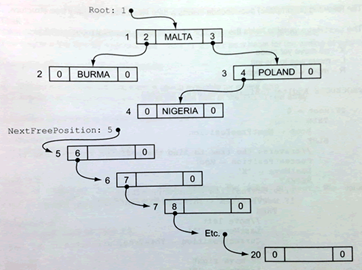
\includegraphics[width=0.5\paperwidth]{C:/Users/Admin/Desktop/Github/question_bank/LyX/static/img/9597-ALVL-2013-P1-Q3}
\par\end{center}

The diagram shows the binary tree and linked list after four values
have been added.

\subsubsection*{Task 3.1}

Write the program code to declare all the required variables and create
the initial linked list which contains all 20 nodes. Add statement(s)
to initialise the empty tree.

\hfill{}{[}10{]}

\subsubsection*{Evidence 7}

Your program code for Task 3.1. {[}11{]}

The following (incomplete) pseudocode inserts a data value into the
binary tree structure.

The \texttt{LastMove} variable holds the direction of the previous
traversal move as follows:

X - no move yet made 

L - move was to the left 

R - move was to the right

\noindent %
\noindent\begin{minipage}[t]{1\columnwidth}%
\texttt{PROCEDURE AddItemToBinaryTree(NewFreeItem)}

\texttt{\qquad{}IF Root = 0}

\texttt{\qquad{}\qquad{}THEN}

\texttt{\qquad{}\qquad{}\qquad{}Root \textleftarrow{} NextFreePosition}

\texttt{\qquad{}\qquad{}ELSE}

\texttt{\qquad{}\qquad{}\qquad{}// traverse the tree to find the
position for the new value}

\texttt{\qquad{}\qquad{}\qquad{}CurrentPosition \textleftarrow{}
Root}

\texttt{\qquad{}\qquad{}\qquad{}LastMove \textleftarrow{} 'X'}

\texttt{\qquad{}\qquad{}\qquad{}REPEAT}

\texttt{\qquad{}\qquad{}\qquad{}\qquad{}PreviousPosition \textleftarrow{}
CurrentPosition}

\texttt{\qquad{}\qquad{}\qquad{}\qquad{}IF NewFreeItem < ThisTree{[}CurrentPosition{]}.Data}

\texttt{\qquad{}\qquad{}\qquad{}\qquad{}\qquad{}THEN}

\texttt{\qquad{}\qquad{}\qquad{}\qquad{}\qquad{}\qquad{}// move
left}

\texttt{\qquad{}\qquad{}\qquad{}\qquad{}\qquad{}\qquad{}LastMove
\textleftarrow{} 'L'}

\texttt{\qquad{}\qquad{}\qquad{}\qquad{}\qquad{}\qquad{}CurrentPosition
\textleftarrow{} ThisTree{[}CurrentPosition{]}.LeftP}

\texttt{\qquad{}\qquad{}\qquad{}\qquad{}\qquad{}ELSE}

\texttt{\qquad{}\qquad{}\qquad{}\qquad{}\qquad{}\qquad{}// move
right}

\texttt{\qquad{}\qquad{}\qquad{}\qquad{}\qquad{}\qquad{}LastMove
\textleftarrow{} 'R'}

\texttt{\qquad{}\qquad{}\qquad{}\qquad{}\qquad{}\qquad{}CurrentPosition
\textleftarrow{} ThisTree{[}CurrentPosition{]}.RightP}

\texttt{\qquad{}\qquad{}\qquad{}\qquad{}ENDIF}

\texttt{\qquad{}\qquad{}\qquad{}UNTIL CurrentPosition = 0}

\texttt{\qquad{}ENDIF}

\texttt{\qquad{}IF LastMove = 'R'}

\texttt{\qquad{}\qquad{}THEN}

\texttt{\qquad{}\qquad{}\qquad{}ThisTree{[}PreviousPosition{]}.RightP
\textleftarrow{} NextFreePosition}

\texttt{\qquad{}\qquad{}ELSE}

\texttt{\qquad{}\qquad{}\qquad{}ThisTree{[}PreviousPosition{]}.LeftP
\textleftarrow{} NextFreePosition}

\texttt{\qquad{}ENDIF}

\texttt{\qquad{}NextFreePosition ThisTree{[}NextFreePosition{]}.LeftP}

\texttt{ENDPROCEDURE}%
\end{minipage}

Note: The above text is available in the text file \texttt{PSEUDOCODE\_TASK\_3\_2.TXT}

\subsubsection*{Task 3.2}

Write non-recursive code to implement the \texttt{AddItemToBinaryTree}
procedure. You may use the text file \texttt{PSEUDOCODE\_TASK\_3\_2.TXT}
as a basis for the writing of your code.

The given pseudocode is incomplete as:
\begin{itemize}
\item it does not initially test that there is space available for a new
item 
\item it does not assign \texttt{NewTreeItem} to the data field of the \texttt{ThisTree}
array
\end{itemize}
Add these requirements to your program solution.

\subsubsection*{Evidence 8}

Your program code for Task 3.2.\hfill{} {[}6{]}

\subsubsection*{Task 3.3}

Write a procedure\texttt{ OutputData} which displays the value of
\texttt{Root}, the value of \texttt{NextFreePosition} and the contents
of \texttt{ThisTree} in index order.

\subsubsection*{Evidence 9}

Your program code for Task 3.3. \hfill{}{[}5{]}

\subsubsection*{Task 3.4}

Write a main program to:
\begin{itemize}
\item Input new data items and add them to the binary tree by calling procedure
\texttt{AddItemToBinaryTree}. The input is terminated with value \textquotedbl\texttt{XXX}\textquotedbl .
Do not attempt to validate the input of the country names. 
\item Your program will then call procedure \texttt{OutputData}.
\end{itemize}
Run the program with the input of the single value \textquotedbl\texttt{XXX}\textquotedbl .

\subsubsection*{Evidence 10}

Screenshot showing the output from running the program in Task 3.4.\hfill{}
{[}3{]}

\subsubsection*{Task 3.5}

Test your program using the following data items input in the order
shown:
\begin{center}
\texttt{INDIA, NEPAL, MALAYSIA, SINGAPORE, BURMA, CANADA, LATVIA,
XXX}
\par\end{center}

\subsubsection*{Evidence 11}

Provide screenshot test evidence for Task 3.5. \hfill{}{[}5{]}

Further program code is required to carry out an \textbf{in-order
traversal}.

\subsubsection*{Task 3.6}

Write a recursive procedure to carry out an in-order tree traversal. 

Include a call to the procedure from your main program.

\subsubsection*{Evidence 12}

Your program code. \hfill{}{[}8{]}

\subsubsection*{Evidence 13}

Produce a screenshot for the Task 3.5 dataset confirming the output
of the countries in alphabetical order. \hfill{}{[}2{]}

 \newpage 

\quad{}
\item \textbf{{[}ALVL/9597/2013/P1/Q4{]} }

The task is to input data for a frequency distribution and then output
to the screen a horizontal bar chart.

The data is input as an X value followed by its frequency. Assume
the frequency is always in the range 0 to 60 and there are no more
than six X values.

The input shown below shows the number of sweatshirts sold in a retail
shop over a one week period; for example there were 39 XL items sold

\noindent\fbox{\begin{minipage}[t]{1\columnwidth - 2\fboxsep - 2\fboxrule}%
\texttt{Next X value ... <ZZZ to END> XS }

\texttt{Frequency ... 12 }

\texttt{Next X value ... <ZZZ to END> S }

\texttt{Frequency ... 22 }

\texttt{Next X value ... <ZZZ to END> M }

\texttt{Frequency ... 45 }

\texttt{Next X value ... <ZZZ to END> L }

\texttt{Frequency ... 56 }

\texttt{Next X value ... <ZZZ to END> XL }

\texttt{Frequency ... 39 }

\texttt{Next X value ... <ZZZ to END> XXL}

\texttt{Frequency ... 11 }

\texttt{Next X value ... <ZZZ to END> ZZZ}

\texttt{++++++++++++++++++++++++++++++++++++++++}

\texttt{Frequency distribution }

\texttt{++++++++++++++++++++++++++++++++++++++++}

\texttt{XS ~@@@@@@@@@@@@ }

\texttt{S ~~@@@@@@@@@@@@@@@@@@@@@@ }

\texttt{M ~~@@@@@@@@@@@@@@@@@@@@@@@@@@@@@@@@@@@@@@@@@@@@@ }

\texttt{L ~~@@@@@@@@@@@@@@@@@@@@@@@@@@@@@@@@@@@@@@@@@@@@@@@@@@@@@@@@ }

\texttt{XL ~@@@@@@@@@@@@@@@@@@@@@@@@@@@@@@@@@@@@@@@ }

\texttt{XXL @@@@@@@@@@@}%
\end{minipage}}

\subsubsection*{Task 4.1}

Write a program which inputs a set of X values and frequencies and
produces output in the format shown.

\subsubsection*{Evidence 14}

Your program code for Task 4.1.\hfill{}{[}8{]}

\subsubsection*{Evidence 15}

A screenshot to confirm the dataset used and the output produced.
\hfill{}{[}2{]}

The appearance of the bar chart display is to be improved as follows:
\begin{itemize}
\item Each bar is to be represented by more than one line of the same character
to that its bar width is increased. 
\item Each bar will be shown with the same number of lines. 
\item The complete bar chart, including the heading, is to take up no more
than 40 lines. 
\item The line width for the output is exactly 80 characters. 
\item Its appearance could be improved by changing the @ character.
\end{itemize}

\subsubsection*{Task 4.2}

Write code to produce a new chart for the data used in Task 4.1 showing
the maximum possible bar width and any other refinements you have
introduced.

\subsubsection*{Evidence 16}

Your program code for Task 4.2. \hfill{}{[}4{]}

\subsubsection*{Evidence 17}

A screenshot showing the data entry followed by the bar chart. \hfill{}{[}2{]}

Some datasets will have a frequency which is greater than 60 and so
the frequencies of the dataset can no longer be shown with a corresponding
number of characters in the line. The frequencies will need to be
scaled before the output is attempted.

The bar chart would benefit by the inclusion of a horizontal axis
labelled with a scale showing the frequency values.

\subsubsection*{Task 4.3}

Revise your program code to meet these new requirements.

\subsubsection*{Evidence 18}

Your program code for Task 4.3.\hfill{} {[}8{]}

\subsubsection*{Evidence 19}

Screenshots demonstrating: 
\begin{itemize}
\item Dataset 1 as used in Task 4.1 which needs no scaling 
\item Dataset 2 of your choice to demonstrate frequencies which must be
scaled 
\item Dataset 3 of your choice to demonstrate frequencies which must be
scaled differently to Dataset 2 
\end{itemize}
\hfill{}{[}6{]}

 \newpage 

\item \textbf{{[}ALVL/9597/2013/P2/Q1{]} }

A dental practice currently uses a computer system to store details
of its patients, staff and appointments in separate files.

The practice manager and the receptionist have their own computers
for accessing and updating the files.

The system produces a small number of reports.

An updated system is to be produced by a software company. The updated
system will use a database. In the updated system the dentists will
be given a hand-held device to use in their rooms for accessing and
updating the patient records. The new system will also be capable
of producing additional reports.

The software company has software engineers who have expert skills
in specific areas of software development. A number of the engineers
will be involved in the development of the updated system.
\begin{enumerate}
\item Describe and justify three methods which can be used to determine
what further reports are required from the updated computer system.
{[}6{]}
\item The work to update the system is partly managed by the following Program
Evaluation and Review Technique (PERT) chart.

A - investigation 

B - analysis 

C - design of database 

D - design of reports 

E - design of screen displays for dentists 

F - transfer of data from files into database 

G - documentation produced 

H - acceptance testing 

I - hand over to customer

Time is measured in weeks.
\begin{center}
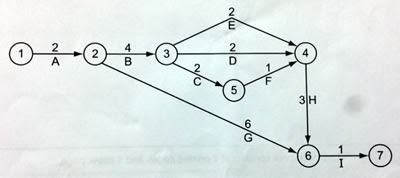
\includegraphics[width=0.5\paperwidth]{C:/Users/Admin/Desktop/Github/question_bank/LyX/static/img/9597-ALVL-2013-P2-Q1-1}
\par\end{center}
\begin{enumerate}
\item State the critical path.\hfill{} {[}1{]}
\item State the minimum time in which the updated system could be operational.
\hfill{}{[}1{]}
\item For activity E state the 
\begin{itemize}
\item earliest Start time 
\item earliest Finish time 
\item latest Start time
\item latest Finish time\hfill{}{[}4{]}
\end{itemize}
\end{enumerate}
\item {}\textcolor{white}{\_}
\begin{center}
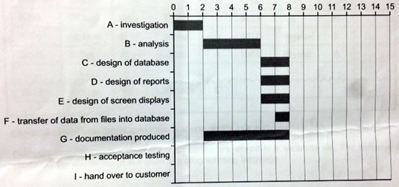
\includegraphics[width=0.5\paperwidth]{C:/Users/Admin/Desktop/Github/question_bank/LyX/static/img/9597-ALVL-2013-P2-Q1-2}
\par\end{center}

The Gantt chart above is based on the information in part \textbf{(b)}.
The timing of two activities is missing and also the timing of one
of the activities shown is incorrect.

Draw a sketch of the Gantt chart to show the correct version. \hfill{}{[}4{]}
\item Explain how the Gantt chart can help with the work that the software
engineers have to carry out. \hfill{}{[}2{]}
\item A small team is put together to consider security aspects of the updated
system.
\begin{enumerate}
\item Identify \textbf{two} possible members of the team and justify your
choice.\hfill{} {[}4{]}
\end{enumerate}
The team have to produce a report to which they all make a contribution.
The report is stored on a network. Each member of the team has access
to allow them to add their contribution.
\begin{enumerate}
\item[ii]  Give \textbf{two} examples of unethical behaviour by a team member.\hfill{}
{[}2{]}
\end{enumerate}
\item Name and describe \textbf{two} types of documentation produced for
this project.\hfill{} {[}6{]}

\noindent\fbox{\begin{minipage}[t]{1\columnwidth - 2\fboxsep - 2\fboxrule}%
End-User documentation 
\begin{itemize}
\item for actual users of system to learn about features and how to use
them 
\item minimum/recommended hardware and software system requirements (operating
system, version, processor, amount of RAM and hard disk space, etc.) 
\item installation guide + step by step guide of how to perform a task or
use a feature 
\item frequently asked questions (FAQ) for common troubleshooting problems
and solutions 
\item support contact information, safety instructions, warranty information
\end{itemize}
Technical documentation
\begin{itemize}
\item for developers to document technical requirements and features of
system
\item system objectives and scope 
\item input and output/report specifications 
\item data storage/database specification 
\item modules/processes and algorithms 
\item user interfaces and application programming interfaces (APIs) 
\item testing
\item implementation/deployment 
\item bugs report and known issues
\end{itemize}
%
\end{minipage}}
\end{enumerate}
The hand-held devices the dentists use in their practice rooms will
be networked. Both client-side scripting and server-side scripting
will be used in the new software which is produced. An intranet with
a web server will be created. Web browsers will be used on the hand-held
devices.
\begin{enumerate}
\item[(g)]  Describe three possible uses of the device.\hfill{} {[}6{]}
\item[(h)]  For each scripting method, client-side scripting and server-side
scripting, give an appropriate example. Justify your response.\hfill{}
{[}4{]}
\end{enumerate}

 \newpage 

\item \textbf{{[}ALVL/9597/2013/P2/Q2{]} }

Examination centres receive examination results for their candidates
as a printed report. The report lists the candidates in order based
on their Index Number. For each candidate their results occupy one
row of the report. Each row displays the results for all subjects
that the candidate sat in the examination.
\begin{center}
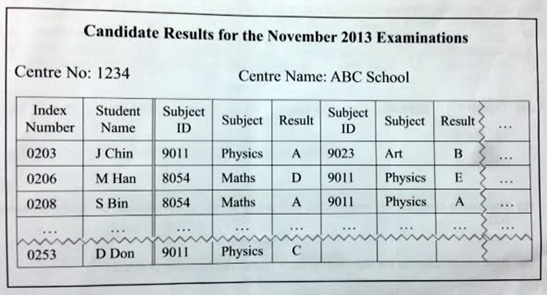
\includegraphics[width=0.5\paperwidth]{C:/Users/Admin/Desktop/Github/question_bank/LyX/static/img/9597-ALVL-2013-P2-Q2-1}
\par\end{center}

Candidates can only take examinations at one centre in a particular
session.

Currently the candidate results for each centre are stored in a separate
file. The software that produces the above report is written in a
programming language.
\begin{enumerate}
\item Describe, using an example, why this file has data redundancy.\hfill{}
{[}2{]}
\item An extra field is added to the file, but the report will not include
this new field. 

Describe the problem that will arise. \hfill{}{[}3{]}
\end{enumerate}
A normalised database solution to this problem is designed, which
has a number of tables.
\begin{enumerate}
\item[(c)]  Draw an E-R diagram that shows these tables and the relationships
between them.\hfill{} {[}5{]}
\item[(d)]  When the data are stored in a database, privacy is of great concern.

Explain why.\hfill{} {[}2{]}
\end{enumerate}

 \newpage 

\item \textbf{{[}ALVL/9597/2013/P2/Q3{]} }

A hash table has an index range of 1 to 900. The following pseudocode
describes an algorithm for searching the table using the hashing function
Hash. It is assumed that the key is present in the table.

\noindent %
\noindent\begin{minipage}[t]{1\columnwidth}%
\texttt{01 Index <- Hash(Key) }

\texttt{02 WHILE Table{[}Index, 1{]} <> Key }

\texttt{03 \qquad{}Index <- Index + 1 }

\texttt{04 ENDWHILE }

\texttt{05 Value <- Table{[}Index, 2{]}}%
\end{minipage}
\begin{enumerate}
\item Explain the purpose of:
\begin{enumerate}
\item line 3
\item line 5\hfill{} {[}4{]}
\end{enumerate}
\item Describe a problem that might occur with a key which, when hashed,
produces an index of 900. \hfill{}{[}2{]}
\item What modification to the algorithm is required to overcome this problem?
\hfill{}{[}3{]}
\item Explain how a new item can be added to this hash table. \hfill{}{[}4{]}
\end{enumerate}

 \newpage 

\item \textbf{{[}ALVL/9597/2013/P2/Q4{]} }

A software development company currently hosts its own email server.
The company is considering a replacement webmail service, using cloud
computing.
\begin{enumerate}
\item (a) State two advantages of this change.\hfill{} {[}2{]}
\item (b) State one disadvantage of this change. \hfill{}{[}1{]}
\end{enumerate}
The company is also considering other uses of the cloud. These include
collaborative activities between employees of the company and also
assistance in developing new software.
\begin{enumerate}
\item[(c)]  Describe an example of how employees of the company may use the
cloud to work collaboratively.\hfill{} {[}3{]}
\item[(d)]  Describe how the cloud can be beneficial to the company when developing
new software for a client. \hfill{}{[}4{]}
\end{enumerate}

 \newpage 

\item \textbf{{[}ALVL/9597/2013/P2/Q5{]} }

Bank customers are allowed to withdraw money from their accounts at
an ATM. They cannot withdraw more than the current balance in their
account. There is a daily limit on the amount that can be withdrawn.
In some circumstances a charge is made for the transaction. The rules
are:
\begin{itemize}
\item the transaction is rejected if the withdrawal amount requested is
greater than the current balance 
\item the transaction is rejected if the withdrawal amount exceeds the daily
limit 
\item if the current balance before the transaction is carried out is less
than 50 dollars then any successful transaction incurs a fixed charge
\end{itemize}
\begin{enumerate}
\item Create a decision table showing all the possible conditions and actions.
\hfill{}{[}4{]}
\item Simplify your decision table by removing redundancies. \hfill{}{[}4{]}
\item Using your answer in (b) write a function using pseudocode. The function
returns:
\begin{itemize}
\item -1 to indicate a rejection; 
\item 0 for a charge-free successful transaction; 
\item the charge for a chargeable successful transaction.\hfill{} {[}5{]}
\end{itemize}
\item State two ways in which your answer in (c) demonstrates clarity of
code. \hfill{}{[}2{]}
\end{enumerate}

 \newpage 

\item \textbf{{[}ALVL/9597/2013/P2/Q6{]} }

The ASCII code for the character 'Z', expressed as a denary integer,
is 90.
\begin{enumerate}
\item Express the denary integer 90 as:
\begin{enumerate}
\item an eight-bit binary number
\item a hexadecimal number \hfill{}{[}2{]}
\end{enumerate}
\item Give two reasons why hexadecimal numbers are used in computing. \hfill{}{[}2{]}
\item State the ASCII code for 'X' in denary. Explain your answer.\hfill{}
{[}2{]}
\item Explain why the Unicode encoding system has replaced ASCII. \hfill{}{[}2{]}
\item Describe a method of storing strings of characters of variable length
in a computer. \hfill{}{[}2{]}
\end{enumerate}

 \newpage 

\item \textbf{{[}ALVL/9597/2019/P1/Q1{]} }

Many applications require the user to search for a data item from
a file or one-dimensional array.

\texttt{JARGON.TXT} is a text file containing computing terms with
one term per line. The program will read all the terms from \texttt{JARGON.TXT}
into an array.

The user will choose if the type of search is to find:
\begin{enumerate}
\item[1.]  An exact match 
\item[2.]  A match at the beginning of the term text
\item[3.]  A match anywhere within the term text
\end{enumerate}

\subsubsection*{Task 1.1}

Design and write program code to:
\begin{itemize}
\item Read the entire contents of \texttt{JARGON.TXT} into an array 
\item Allow the user to repeatedly select the type of search, then input
a term 
\item Output the matching term(s) found 
\item Output a count of the number of matches 
\item End with the input of term \textquotedbl XXX\textquotedbl{}
\end{itemize}
A typical run of the program is shown below:

\texttt{+++++++++++++++++++++++ }

\texttt{1. Exact match }

\texttt{2. Start of term }

\texttt{3. Within term }

\texttt{++++++++++++++++++ }

\texttt{Choice ?1 }

\texttt{Term?firewall }

\texttt{firewall }

\texttt{There were 1 matching term(s)}

\texttt{+++++++++++++++++++++++ }

\texttt{1. Exact match }

\texttt{2. Start of term }

\texttt{3. Within term }

\texttt{++++++++++++++++++ }

\texttt{Choice ?2 }

\texttt{Term?data }

\texttt{data flow diagram }

\texttt{database management system }

\texttt{data file }

\texttt{database }

\texttt{There were 4 matching term(s)}

\texttt{+++++++++++++++++++++++ }

\texttt{1. Exact match }

\texttt{2. Start of term }

\texttt{3. Within term }

\texttt{++++++++++++++++++}

\texttt{Choice ?3 }

\texttt{Term?box }

\texttt{white box testing }

\texttt{black box testing }

\texttt{There were 2 matching term(s)}

\subsubsection*{Evidence 1}

The program code. \hfill{}{[}11{]}

\subsubsection*{Task 1.2}

Study the contents of \texttt{JARGON.TXT} and then design four test
cases to thoroughly test the working of your program code.

\subsubsection*{Evidence 2}

State the test data used in Task 1.2 and show screenshots to confirm
the successful testing of each of your four test cases. \hfill{}{[}4{]}

 \newpage 

\item \textbf{{[}ALVL/9597/2019/P1/Q2{]} }

A binary search (binary chop) is a technique to search for a value
in an ordered dataset.

\subsubsection*{Task 2.1}

Study the identifier table and incomplete recursive algorithm. 

The missing parts of the algorithm are labelled A, B and C.
\begin{center}
\begin{tabular}{|l|c|l|}
\hline 
\texttt{\hspace{0.01\columnwidth}}Variable & \texttt{\hspace{0.01\columnwidth}}Data Type & \texttt{\hspace{0.05\columnwidth}}Description\tabularnewline
\hline 
\texttt{ThisArray} & \texttt{ARRAY OF STRING} & Array containing the the dataset\tabularnewline
\hline 
\texttt{FindValue} & \texttt{STRING} & Item to be found\tabularnewline
\hline 
\texttt{Low} & \texttt{INTEGER} & Lowest index of the considered list\tabularnewline
\hline 
\texttt{High} & \texttt{INTEGER} & Highest index of the considered list\tabularnewline
\hline 
\texttt{Middle} & \texttt{INTEGER} & The array index for the middle position of the current list considered\tabularnewline
\hline 
\end{tabular}
\par\end{center}

\noindent %
\noindent\begin{minipage}[t]{1\columnwidth}%
\texttt{FUNCTION BinarySearch(ThisArray, FindValue, Low, High) RETURNS
INTEGER}

\texttt{\qquad{}DECLARE Middle : INTEGER}

\texttt{\qquad{}IF ............... A ...............}

\texttt{\qquad{}\qquad{}THEN}

\texttt{\qquad{}\qquad{}\qquad{}RETURN -1 // not found}

\texttt{\qquad{}ELSE}

\texttt{\qquad{}\qquad{}// calculate new Middle value}

\texttt{\qquad{}\qquad{}Middle \textleftarrow{} ............... B
...............}

\texttt{\qquad{}\qquad{}IF ThisArray{[}Middle{]} > FindValue}

\texttt{\qquad{}\qquad{}\qquad{}THEN}

\texttt{\qquad{}\qquad{}\qquad{}\qquad{}RETURN BinarySearch(ThisArray,
FindValue, Low, Middle - 1)}

\texttt{\qquad{}\qquad{}\qquad{}ELSE}

\texttt{\qquad{}\qquad{}\qquad{}\qquad{}IF ThisArray{[}Middle{]}
< FindValue}

\texttt{\qquad{}\qquad{}\qquad{}\qquad{}\qquad{}THEN}

\texttt{\qquad{}\qquad{}\qquad{}\qquad{}\qquad{}\qquad{}............... C
...............}

\texttt{\qquad{}\qquad{}\qquad{}\qquad{}\qquad{}ELSE}

\texttt{\qquad{}\qquad{}\qquad{}\qquad{}\qquad{}\qquad{}RETURN
Middle // found at position Middle}

\texttt{\qquad{}\qquad{}\qquad{}\qquad{}ENDIF}

\texttt{\qquad{}\qquad{}ENDIF}

\texttt{\qquad{}ENDIF}

\texttt{ENDFUNCTION}%
\end{minipage}

\subsubsection*{Evidence 3}

What are the three missing lines in this pseudocode? \hfill{}{[}3{]}

\subsubsection*{Task 2.2}

Write a program to implement binary search. 

The program will
\begin{itemize}
\item Call procedure InitialiseAnimals 
\item Input an animal name
\item Use the function BinarySearch 
\item Report whether or now this animal name was found. If found, also output
the index position.
\end{itemize}
The array in the program has identifier \texttt{MyAnimal}. 

Use the dataset given in the file \texttt{ANIMALS.TXT}. You should
paste the contents of this file into your program. The statements
will form the basis of the code for the procedure \texttt{InitialiseAnimals}.

\subsubsection*{Evidence 4}

Program code for Task 2.2 \hfill{}{[}7{]}

\subsubsection*{Evidence 5}

Screenshot to confirm that an animal wich is present in the list was
found with its index position displayed. \hfill{}{[}1{]}

\subsubsection*{Task 2.3}

Amend the program as follows: 

The program must also output the number of function calls carried
out.

\subsubsection*{Evidence 6}

The amended program code. \hfill{}{[}4{]}

\subsubsection*{Evidence 7}

Screenshots showing the amended ouput for runs of the program where: 
\begin{itemize}
\item the animal is found
\item the animal is not found. \hfill{}{[}2{]}
\end{itemize}

 \newpage 

\item \textbf{{[}ALVL/9597/2019/P1/Q3{]} }

A program is to be written to represent and implement a linked list
of nodes. Each node contains a string data value and a pointer. The
pointers link the data items in alphabetical order. 

The unused nodes are linked as shown below. The first unused node
is the position where the next new data item is to be stored. 
\begin{center}
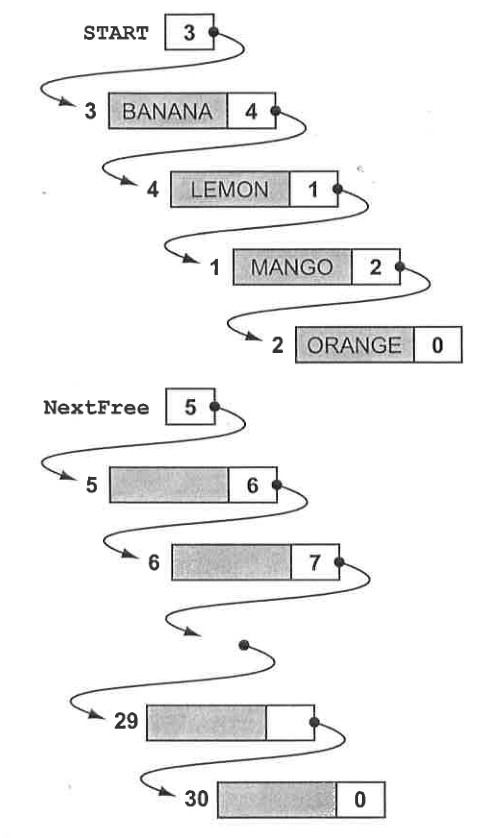
\includegraphics[width=0.25\paperwidth]{C:/Users/Admin/Desktop/Github/question_bank/LyX/static/img/9597-ALVL-2014-P1-Q3}
\par\end{center}

The diagram shows the linked list with: 
\begin{itemize}
\item the items MANGO, ORANGE, BANANA and LEMON (added in that order). 
\item the unused nodes linked together.
\end{itemize}
Each node is implemented as an instance of the class\texttt{ ListNode}.
The class \texttt{ListNode} has the following properties: 
\begin{center}
\begin{tabular}{|l|c|l|}
\hline 
\multicolumn{3}{|c|}{Class\texttt{: ListNode}}\tabularnewline
\hline 
\multicolumn{3}{|c|}{Properties}\tabularnewline
\hline 
\texttt{\hspace{0.01\columnwidth}}Identifier & \texttt{\hspace{0.01\columnwidth}}Data Type & \texttt{\hspace{0.01\columnwidth}}Description\tabularnewline
\hline 
\texttt{DataValue} & \texttt{STRING} & The node data\tabularnewline
\hline 
\texttt{PointerValue} & \texttt{INTEGER} & The node pointer\tabularnewline
\hline 
\end{tabular}
\par\end{center}

A linked list is implemented as an instance of the class \texttt{LinkedList}.
The class \texttt{LinkedList} has the following properties and methods: 
\begin{center}
\begin{tabular}{|l|c|>{\raggedright}p{0.25\columnwidth}|}
\hline 
\multicolumn{3}{|c|}{Class\texttt{: LinkedList}}\tabularnewline
\hline 
\multicolumn{3}{|c|}{Properties}\tabularnewline
\hline 
\texttt{\hspace{0.01\columnwidth}}Identifier & \texttt{\hspace{0.01\columnwidth}}Data Type & \texttt{\hspace{0.01\columnwidth}}Description\tabularnewline
\hline 
\texttt{Node} & \texttt{ARRAY{[}30{]} OF ListNode} & The linked list data structure --- data values and pointers.The array
index starts at 1.For testing purposes the dataset has a maximum of
30 items.\tabularnewline
\hline 
\texttt{Start} & \texttt{INTEGER} & Index position of the node at the start of the linked list\tabularnewline
\hline 
\texttt{NextFree} & \texttt{INTEGER} & Index position of the next unused node \tabularnewline
\hline 
\multicolumn{3}{|l|}{Methods}\tabularnewline
\hline 
\texttt{\hspace{0.01\columnwidth}}Identifier &  & \texttt{\hspace{0.01\columnwidth}}Description\tabularnewline
\hline 
\texttt{Initialise} & \texttt{PROCEDURE} & Sets all the node data values to \textquoteleft empty string\textquoteright .

Set pointers to indicate all nodes are unused and linked.

lnitialise values for \texttt{Start} and \texttt{NextFree}.\tabularnewline
\hline 
\texttt{AddNode} & \texttt{PROCEDURE} & Add a new data item to the linked list.\tabularnewline
\hline 
\texttt{Traversal} & \texttt{PROCEDURE} & Display the data items in order.\tabularnewline
\hline 
\texttt{ReverseTraversal} & \texttt{PROCEDURE} & Display the data items in reverse order.\tabularnewline
\hline 
\texttt{DisplayLinkedList} & \texttt{PROCEDURE} & Display the current state of pointers and the array contents.\tabularnewline
\hline 
\texttt{IsEmpty} & \texttt{FUNCTION RETURNS BOOLEAN} & Tests for empty linked list.\tabularnewline
\hline 
\texttt{IsFull} & \texttt{FUNCTION RETURNS BOOLEAN} & Tests for no unused nodes.\tabularnewline
\hline 
\end{tabular}
\par\end{center}

\subsubsection*{Task 3.1}

Write program code that repeatedly:
\begin{itemize}
\item displays a menu with the following choices: 
\begin{enumerate}
\item[1.]  Add an item 
\item[2.]  Traverse the linked list of used nodes and output the data values 
\item[3.]  Output all pointers and data values 
\item[4.]  Exit 
\end{enumerate}
\item calls an appropriate procedure depending on the user's choice. 
\end{itemize}

\subsubsection*{Evidence 8}

Program code for Task 3.1.\hfill{} {[}5{]}

\subsubsection*{Task 3.2}

Write program code for the classes \texttt{ListNode} and \texttt{LinkedList}
including the \texttt{IsEmpty} method. The code should follow the
specification given. 

Do not attempt to write the methods \texttt{AddNode}, \texttt{Traversal},
\texttt{ReverseTraversal} or \texttt{IsFull} at this stage. 

\subsubsection*{Evidence 9}

Program code for the \texttt{ListNode} and \texttt{LinkedList} classes
(Task 3.2).\hfill{} {[}12{]}

\subsubsection*{Task 3.3}

Write code to create a \texttt{LinkedList} object in the main program.

Run the program and select menu choice 3 to confirm the initial values
of the pointers and data values when the linked list is empty. {[}10{]}

\subsubsection*{Evidence 10}

Screenshot confirming all values after initialisation of the \texttt{LinkedList}
object (Task 3.3). 

\hfill{} {[}3{]}

\subsubsection*{Task 3.4}

Consider the \texttt{AddNode} method. The following algorithm will
add a new data item to the linked list. 

The algorithm uses the variables below:
\begin{center}
\begin{tabular}{|l|c|>{\raggedright}p{0.25\columnwidth}|}
\hline 
\texttt{\hspace{0.01\columnwidth}}Identifier & \texttt{\hspace{0.01\columnwidth}}Data Type & \texttt{\hspace{0.01\columnwidth}}Description\tabularnewline
\hline 
\texttt{NewItem} & \texttt{STRING} & New data item input by the user\tabularnewline
\hline 
\texttt{Found} & \texttt{BOOLEAN} & Flags to \texttt{TRUE} when the position at which to insert the new
item has been found\tabularnewline
\hline 
\texttt{Current} & \texttt{INTEGER} & Current array index position during list traversal\tabularnewline
\hline 
\texttt{Previous} & \texttt{INTEGER} & Previous array index position during list traversal\tabularnewline
\hline 
\texttt{Temp} & \texttt{INTEGER} & Temporary storage of pointer value\tabularnewline
\hline 
\end{tabular}
\par\end{center}

\noindent\fbox{\begin{minipage}[t]{1\columnwidth - 2\fboxsep - 2\fboxrule}%
\texttt{PROCEDURE AddNode }

\texttt{\qquad{}INPUT NewItem }

\texttt{\qquad{}Node{[}NextFree{]}.DataValue <\textemdash{} NewItem }

\texttt{\qquad{}IF Start = 0 }

\texttt{\qquad{}\qquad{}THEN }

\texttt{\qquad{}\qquad{}Start <\textemdash{} NextFree }

\texttt{\qquad{}\qquad{}Temp <\textemdash{} Node{[}NextFree{]}.PointerValue }

\texttt{\qquad{}\qquad{}Node{[}NextFree{]}.PointerValue <\textemdash{}
0 }

\texttt{\qquad{}\qquad{}NextFree <\textemdash{} Temp }

\texttt{\qquad{}ELSE }

\texttt{\qquad{}\qquad{}// traverse the list - starting at Start
to find }

\texttt{\qquad{}\qquad{}// the position at which to insert the new
item }

\texttt{\qquad{}\qquad{}Temp <\textemdash{} Node{[}NextFree{]}.PointerValue }

\texttt{\qquad{}\qquad{}IF NewItem < Node{[}Start{]}.DataValue }

\texttt{\qquad{}\qquad{}\qquad{}THEN }

\texttt{\qquad{}\qquad{}\qquad{}\qquad{}// new item will become
the start of the list }

\texttt{\qquad{}\qquad{}\qquad{}\qquad{}Node{[}NextFree{]}.PointerValue
<\textemdash{} Start }

\texttt{\qquad{}\qquad{}\qquad{}\qquad{}Start <\textemdash{} NextFree }

\texttt{\qquad{}\qquad{}\qquad{}\qquad{}NextFree <\textemdash{}
Temp }

\texttt{\qquad{}\qquad{}\qquad{}ELSE }

\texttt{\qquad{}\qquad{}\qquad{}\qquad{}// the new item is not
at the start of the list }

\texttt{\qquad{}\qquad{}\qquad{}\qquad{}Previous <\textemdash{}
0 }

\texttt{\qquad{}\qquad{}\qquad{}\qquad{}Current <\textemdash{}
Start }

\texttt{\qquad{}\qquad{}\qquad{}\qquad{}Found <\textemdash{} False }

\texttt{\qquad{}\qquad{}\qquad{}\qquad{}REPEAT }

\texttt{\qquad{}\qquad{}\qquad{}\qquad{}\qquad{}IF NewItem <=
Node{[}Current{]}.DataValue }

\texttt{\qquad{}\qquad{}\qquad{}\qquad{}\qquad{}\qquad{}THEN }

\texttt{\qquad{}\qquad{}\qquad{}\qquad{}\qquad{}\qquad{}\qquad{}Node{[}Previous{]}.PointerValue
<\textemdash{} NextFree }

\texttt{\qquad{}\qquad{}\qquad{}\qquad{}\qquad{}\qquad{}\qquad{}Node{[}NextFree{]}.PointerValue
<\textemdash{} Current }

\texttt{\qquad{}\qquad{}\qquad{}\qquad{}\qquad{}\qquad{}\qquad{}NextFree
<\textemdash{} Temp }

\texttt{\qquad{}\qquad{}\qquad{}\qquad{}\qquad{}\qquad{}\qquad{}Found
<\textemdash{} True }

\texttt{\qquad{}\qquad{}\qquad{}\qquad{}\qquad{}\qquad{}ELSE }

\texttt{\qquad{}\qquad{}\qquad{}\qquad{}\qquad{}\qquad{}\qquad{}//
move on to the next node }

\texttt{\qquad{}\qquad{}\qquad{}\qquad{}\qquad{}\qquad{}\qquad{}Previous
<\textemdash{} Current }

\texttt{\qquad{}\qquad{}\qquad{}\qquad{}\qquad{}\qquad{}\qquad{}Current
<\textemdash{} Node{[}Current{]}.PointerValue }

\texttt{\qquad{}\qquad{}\qquad{}\qquad{}\qquad{}ENDIF }

\texttt{\qquad{}\qquad{}\qquad{}\qquad{}UNTIL Found = True OR
Current = 0 }

\texttt{\qquad{}\qquad{}\qquad{}\qquad{}IF Current <\textemdash{}
0 }

\texttt{\qquad{}\qquad{}\qquad{}\qquad{}\qquad{}THEN }

\texttt{\qquad{}\qquad{}\qquad{}\qquad{}\qquad{}\qquad{}Node{[}Previous{]}.PointerValue
<\textemdash{} NextFree }

\texttt{\qquad{}\qquad{}\qquad{}\qquad{}\qquad{}\qquad{}Node{[}NextFree{]}.PointerValue
<\textemdash{} 0 }

\texttt{\qquad{}\qquad{}\qquad{}\qquad{}\qquad{}\qquad{}NextFree
<\textemdash{} Temp }

\texttt{\qquad{}\qquad{}\qquad{}\qquad{}ENDIF }

\texttt{\qquad{}\qquad{}ENDIF }

\texttt{\qquad{}ENDIF }

\texttt{ENDPROCEDURE }

Note: The above pseudocode is available in the text file \texttt{PSEUDOCODE\_TASK\_3\_4.TXT}%
\end{minipage}}

Write code to implement for the \texttt{LinkedList} class: 
\begin{itemize}
\item the \texttt{AddNode} method 
\item the \texttt{IsFull} method. 
\end{itemize}
You may use the text file \texttt{PSEUDOCODE\_TASK\_3\_4.TXT} as a
basis for the writing of your code. 

The main program should check each time that the \texttt{LinkedList}
object is not full before using the \texttt{AddNode} method. 

Run the program as follows: 
\begin{itemize}
\item Menu choice 1 four times, inputting the data values: 

MANGO, ORANGE. BANANA. LEMON in that order. 
\item Menu choice 3 to display. 
\end{itemize}

\subsubsection*{Evidence 11}

Program code for method \texttt{AddNode}. \hfill{}{[}8{]}

\subsubsection*{Evidence 12}

Screenshot showing the pointers and the addition of the four nodes
to the linked list.\hfill{} {[}3{]}

\subsubsection*{Task 3.5}

Write program code to implement the \texttt{LinkedList} class method
\texttt{Traversal} by calling the \texttt{TraversalInOrder} procedure
given below. 

\noindent %
\noindent\begin{minipage}[t]{1\columnwidth}%
\texttt{PROCEDURE TraversalInOrder(Index)}

\texttt{\qquad{}IF Index <> 0}

\texttt{\qquad{}\qquad{}THEN}

\texttt{\qquad{}\qquad{}\qquad{}OUTPUT Node{[}lndex{]}.DataValue}

\texttt{\qquad{}\qquad{}\qquad{}// follow the pointer to the next
data item in the linked list}

\texttt{\qquad{}\qquad{}\qquad{}TraversalInOrder(Node{[}Index{]}.PointerValue)}

\texttt{\qquad{}ENDIF}

\texttt{ENDPRCCEDURE}%
\end{minipage}

\subsubsection*{Evidence 13}

Program code for procedures \texttt{Traversal} and \texttt{TraversalInOrder}.\hfill{}
{[}2{]}

\subsubsection*{Task 3.6}

Run the program as follows: 
\begin{itemize}
\item Menu choice 1 four times, inputting the data values: 

MANGO, ORANGE, BANANA. LEMON in that order. 
\item Menu choice 2 to display. 
\end{itemize}

\subsubsection*{Evidence 14}

Screenshot showing the program execution to test the \texttt{Traversal}
method. \hfill{}{[}2{]}

\subsubsection*{Task 3.7}

Make a copy of the \texttt{TraversalInOrder} and \texttt{Traversal}
procedures.

Paste to form two new procedures \texttt{TraversalInReverseOrder}
and \texttt{ReverseTraversal}. 

Make the necessary changes/additions to these procedures in order
that the data items are output in reverse order by calling the new
method \texttt{ReverseTraversal}.

Run the program code from a new menu choice 4.

Test the method using the four items given in Task 3.6.

\subsubsection*{Evidence 15}

Program code for the new procedures. \hfill{}{[}2{]}

\subsubsection*{Evidence 16}

Screenshot showing option 4 selected and the resulting output. \hfill{}{[}1{]}

 \newpage 

\item \textbf{{[}ALVL/9597/2019/P1/Q4{]} }

Design and code a computer program to simulate the following: 

A garden has a rectangular fish pond measuring 15 metres by 8 metres. 

The pond is to be represented on the screen by a rectangular grid.
Each square metre of the pond is represented by an x-coordinate and
a y-coordinate. The top left square metre of the pond display has
x = 1 and y = 1. 

A boy throws a stone into the pond. The user will input the x-coordinate
and y-coordlnate of the stone impact position. 

A grid representing the pond is then displayed with the stone's impact
position: 

\texttt{X coordinate <1 to 15>? 9 }

\texttt{Y coordinate <1 to 8>? 3 }

\texttt{. . . . . . . . . . . . . . . }

\texttt{. . . . . . . . . . . . . . .}

\texttt{. . . . . . . . S . . . . . .}

\texttt{. . . . . . . . . . . . . . .}

\texttt{. . . . . . . . . . . . . . .}

\texttt{. . . . . . . . . . . . . . .}

\texttt{. . . . . . . . . . . . . . .}

\texttt{. . . . . . . . . . . . . . .}

\subsubsection*{Task 4.1}

The following are the suggested characters to use for the visual representation
of the pond: 
\begin{center}
\begin{tabular}{|c|c|l|}
\hline 
Character & ASCII code (decimal) & \texttt{\hspace{0.01\columnwidth}}Represents\tabularnewline
\hline 
. & 46 & One square metre of water\tabularnewline
\hline 
S & 83 & Stone impact position\tabularnewline
\hline 
\end{tabular}
\par\end{center}

Decide on the design to be used for: 
\begin{itemize}
\item The data structure to represent the grid
\item The contents of each square metre of the pond 
\item Procedure(s) and/or function(s)s to be used 
\end{itemize}

\subsubsection*{Evidence 17}

Show your program design (Task 4.1). \hfill{} {[}6{]}

\subsubsection*{Task 4.2}

Write program code to display the pond contents after a single stone
has been thrown. 

\subsubsection*{Evidence 18}

The program code. \hfill{} {[}7{]}

\subsubsection*{Evidence 19}

Screenshot for a single run of the program. \hfill{} {[}1{]}

\subsubsection*{Task 4.3}

The boy has been told to stop throwing stones into the pond because
the pond now has three fish. The fish randomly swim around. Each fish
will occupy a unique grid position.

Using a random number generator, simulate the positioning of the three
fish. 

Use the following character for a fish: 
\begin{center}
\begin{tabular}{|c|c|l|}
\hline 
Character & ASCII code (decimal) & \texttt{\hspace{0.01\columnwidth}}Represents\tabularnewline
\hline 
F & 70 & Fish\tabularnewline
\hline 
\end{tabular}
\par\end{center}

Write program code to show the pond containing the three fish at a
particular instance of time. The program will now only display the
pond and fish. 

\subsubsection*{Evidence 20}

The program code for Task 4.3. \hfill{} {[}6{]}

\subsubsection*{Evidence 21}

Screenshot for a single run of the program. \hfill{} {[}1{]}

\subsubsection*{Task 4.4}

The boy has been asked to feed the fish. He cannot see the fish in
the pond. He throws a food pellet into the pond which lands inside
one of the square metres. If one of the fish is in this square. it
eats the food and becomes a happy fish. 

Use character symbols for the pond\textquoteleft s grid display as
follows: 
\begin{center}
\begin{tabular}{|c|c|l|}
\hline 
Character & ASCII code (decimal) & \texttt{\hspace{0.01\columnwidth}}Represents\tabularnewline
\hline 
. & 46 & One square metre of water\tabularnewline
\hline 
P & 80 & Pellet (if not eaten by one of the fish)\tabularnewline
\hline 
H & 72 & Happy (fed) fish\tabularnewline
\hline 
F & 70 & Fish\tabularnewline
\hline 
\end{tabular}
\par\end{center}

Write program code to simulate the boy throwing one food pellet into
the pond. The user will input an x-coordinate and y-coordinate for
the food pellet position. You should consider the possible reuse of
any code from Tasks 4.2 and 4.3.

\subsubsection*{Evidence 22}

The program code.\hfill{} {[}6{]}

\subsubsection*{Evidence 23}

Screenshotevldence similar to that shown which shows: 
\begin{itemize}
\item one throw which did not feed a fish 

\texttt{X coordinate <1 to 15>? 2 }

\texttt{Y coordinate <1 to 8>? 5 }

\texttt{. . . . . . . . . . . . . . . }

\texttt{. . . . . . . . . . . . . . .}

\texttt{. . . . . . . . F . . . . . .}

\texttt{. . . . . . . . . . . . . . .}

\texttt{. P . . . . . . . . F . . . .}

\texttt{. . . . . . . . . . . . . . .}

\texttt{. . . . F . . . . . . . . . .}

\texttt{. . . . . . . . . . . . . . .}
\item a second throw where a fish was fed 

\texttt{X coordinate <1 to 15>? 1 }

\texttt{Y coordinate <1 to 8>? 5 }

\texttt{. . . . . . . . . . . . . . . }

\texttt{. . . . . . . . . . . . . . .}

\texttt{. . . . . . . . . . . . . . F}

\texttt{. . . . . . . . . . . . . . .}

\texttt{H . . . . . . . . . . . . . .}

\texttt{. . . . . . . . . . . . . . .}

\texttt{. . . . . . . F . . . . . . .}

\texttt{. . . . . . . . . . . . . . .}\hfill{} {[}3{]}
\end{itemize}

 \newpage 

\item \textbf{{[}ALVL/9597/2019/P2/Q1{]} }

A supermarket chain wants to encourage customers to return to its
store. They operate a scheme of rewards for customers based on how
much they spend over a period of time.

Customers are issued with a card that is readable by a Point of Sale
(POS) terminal. When a customer provides their card at the checkout,
the system identifies them and stores the products they purchased
and how much they spent.

Currently the only use of this data is to issue the customer with
vouchers every three months. Vouchers have a value based on the total
amount the customer has spent during the previous three months. The
vouchers can only be used in part payment for goods bought in the
supermarket.

The supermarket managers want to make more use of the customer purchase
data. They hire a software development company to produce software
that will implement new uses of the data.

Software developers have skills in developing software. The supermarket
managers have in depth knowledge of their business. At first, software
developers will have little knowledge of the business.
\begin{enumerate}
\item Explain how the supermarket managers can communicate to the software
developers what they require. \hfill{}{[}2{]}
\item Before designing the new software, the software developers need to
understand the content and structure of the customer purchase data.
Give two methods that can be used for this task, justifying the use
of each. \hfill{}{[}4{]}
\item Once the analysis phase has been completed, describe what decisions
software developers need to make before coding can begin. \hfill{}{[}6{]}
\end{enumerate}
The work to implement new uses of the customer data needs to be managed.
The following Program Evaluation and Review Technique (PERT) chart
is used as a management tool.

Time is measured in weeks. 
\begin{center}
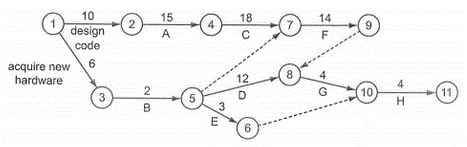
\includegraphics[width=0.7\paperwidth]{C:/Users/Admin/Desktop/Github/question_bank/LyX/static/img/9597-ALVL-2014-P2-Q1}
\par\end{center}
\begin{enumerate}
\item[(d)]  Each activity indicated by a dashed line on the PERT chart is a
dummy activity.
\begin{enumerate}
\item Explain the nature and purpose of a dummy activity.\hfill{} {[}2{]}
\item Each of the following activities matches one of the labels A-H on
the chart.
\begin{itemize}
\item write user documentation 
\item train users 
\item write code 
\item convert files
\item test code 
\item end-user testing 
\item test system 
\item install new hardware
\end{itemize}
Copy and complete the following table, 
\begin{center}
\begin{tabular}{|c|>{\centering}p{0.5\columnwidth}|}
\hline 
Label & Activity\tabularnewline
\hline 
A & \tabularnewline
\hline 
B & \tabularnewline
\hline 
C & \tabularnewline
\hline 
D & \tabularnewline
\hline 
E & \tabularnewline
\hline 
F & \tabularnewline
\hline 
G & \tabularnewline
\hline 
H & \tabularnewline
\hline 
\end{tabular}
\par\end{center}

\hfill{}{[}4{]}
\item Explain the significance of the dummy activity that leads into event
8. \hfill{}{[}3{]}
\end{enumerate}
\item[(e)]  From the PERT chart:
\begin{enumerate}
\item State the critical path.\hfill{} {[}1{]}
\item State the minimum time in which the new software can be developed
and implemented.\hfill{} {[}1{]}
\item The chart omits an activity: \textbf{write technical documentation}.
State a starting point and a finishing point for this activity. Justify
your choices. \hfill{}{[}4{]}
\end{enumerate}
\end{enumerate}
Management staff can already access the company network remotely for
other software applications. Management are to be given the facility
to access, and interact with, the customer data Via the company LAN.
However, a decision is made not to allow access to the customer data
remotely for this updated system.
\begin{enumerate}
\item[(f)]  Describe \textbf{two} methods which can be used to ensure that there
is no remote access to customer data by management staff. \hfill{}{[}4{]}
\end{enumerate}
ln the new system, customers will have access to information through
a web browser. Each customer will be able to see some information
about their purchase history.
\begin{enumerate}
\item[(g)]  Explain what software needs to be developed to provide this customer
facility. \hfill{}{[}5{]}
\item[(h)]  One of the software developers has the task of ensuring that social
issues are considered. This developer has to document these issues. 

Describe \textbf{two} issues that might be in the document with regard
to customers accessing their data. \hfill{}{[}4{]}
\end{enumerate}

 \newpage 

\item \textbf{{[}ALVL/9597/2019/P2/Q2{]} }

Consider the following binary tree:
\begin{center}
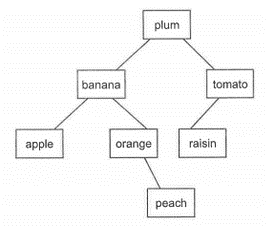
\includegraphics[width=0.35\paperwidth]{C:/Users/Admin/Desktop/Github/question_bank/LyX/static/img/9597-ALVL-2014-P2-Q2}
\par\end{center}
\begin{enumerate}
\item List the nodes, in order, that are visited for a post-order traversal.
\hfill{}{[}2{]}
\item List the nodes, in order, that are visited for an inorder traversal.
\hfill{}{[}2{]}
\item What property is exhibited by the list of items produced in \textbf{part
(b)}? \hfill{}{[}1{]}
\item Describe an algorithm, using pseudocode, to perform a binary tree
search. The output should state whether or not the item is present
in the tree. \hfill{}{[}5{]}
\end{enumerate}

 \newpage 

\item \textbf{{[}ALVL/9597/2019/P2/Q3{]} }

A network manager for a sales company types the following into his
computer:

\texttt{copy C:\textbackslash monthlysales\textbackslash{*}.dat
E\textbackslash :\textbackslash backup\textbackslash junesales
/V}
\begin{enumerate}
\item State the type of user interface being used. \hfill{}{[}1{]}
\item Describe, using the example, two benefits of the user interface named
in \textbf{(a)}. \hfill{}{[}4{]}
\end{enumerate}
The network manager has a disabled user who cannot use a keyboard
but can control a point-and-click device that moves a pointer on the
screen.
\begin{enumerate}
\item[(c)]  Describe a user interface that would allow this user to enter text
into a word processor. \hfill{}{[}3{]}
\item[(d)]  The sales company provides a special user interface for this user.
State\textbf{ two} benefits to the company. \hfill{}{[}2{]}
\end{enumerate}

 \newpage 

\item \textbf{{[}ALVL/9597/2019/P2/Q4{]} }

A small local area network (LAN) in a school consists of one switch,
one file server and ten computers.
\begin{enumerate}
\item Explain why circuit switching could be used in this LAN. \hfill{}{[}2{]}
\end{enumerate}
The network has a connection to the lnternet added.
\begin{enumerate}
\item[(b)] Explain how packet switching is used when a web page is downloaded
from the Internet. \hfill{}{[}3{]}
\end{enumerate}
A packet from the web server consists of 256 bytes. One of the bytes
is the checksum byte. In each byte one bit is the parity bit.
\begin{enumerate}
\item[(c)]  If the byte 0 0 1 1 0 1 0 1 results in a parity error, state the
type of parity being used. \hfill{}{[}1{]}
\item[(d)]  The receiving computer uses the checksum byte to check whether the
packet contains an error. Explain how it does this.\hfill{} {[}4{]}
\end{enumerate}

 \newpage 

\item \textbf{{[}ALVL/9597/2019/P2/Q5{]} }

A software developer is given the task of producing software for a
college. The software will help to manage information about what students
do after finishing at the college.

The destination of each student after college is classified in one
of three possible ways:
\begin{itemize}
\item University
\item Employment 
\item Other
\end{itemize}
The college wishes to store:
\begin{itemize}
\item name 
\item number of A Level passes 
\item destination (U / E / O) 
\item university attended 
\item main subject studied at university 
\item type of employment 
\item what students do when their destination is classified as 'O'
\end{itemize}
The software developer will use an objectoriented approach to developing
a solution.
\begin{enumerate}
\item Draw a class diagram which exhibits the following:
\begin{itemize}
\item suitable classes with appropriate properties and methods 
\item inheritance 
\item polymorphism \hfill{}{[}6{]}
\end{itemize}
\item Explain how your solution to (a) demonstrates software reuse.\hfill{}
{[}2{]}
\end{enumerate}
The data on the students is to be stored in a serial text file called
STUDENT.DAT. Each line of the file has the same structure:

\texttt{<Name><NoOfPasses><Destination><University><MainSubject><EmpType><Other>}

with the string NULL stored where appropriate.
\begin{enumerate}
\item[(c)]  Write an algorithm, in pseudocode, to read data from \texttt{STUDENT.DAT}
and to output the following:
\begin{itemize}
\item total number of students going to university 
\item average number of passes for the students going to university e total
number of students\hfill{} {[}7{]}
\end{itemize}
\end{enumerate}

 \newpage 

\item \textbf{{[}ALVL/9597/2019/P2/Q6{]} }

A function is to be written that returns the sum of all values held
in an array that are greater than a minimum value. The function will
be used with arrays of varying size, but never more than a maximum
of 50 000 elements.

A first attempt at writing the program code for the function is given
below:

\noindent %
\noindent\begin{minipage}[t]{1\columnwidth}%
\texttt{01 FUNCTION TotalSum(Results : ARRAY{[}50000{]} OF REAL, ArraySize
: INTEGER, MinValue : REAL) RETURNS REAL }

\texttt{02 \qquad{}DECLARE Sum, Counter : INTEGER }

\texttt{03 \qquad{}DECLARE Temp : Real }

\texttt{04 \qquad{}Sum = 0.0 }

\texttt{05 \qquad{}\qquad{}FOR Counter = 1 TOO ArraySize }

\texttt{06 \qquad{}\qquad{}\qquad{}Temp = Results{[}Counter{]} }

\texttt{07 \qquad{}\qquad{}\qquad{}IF Temp > MinValue THEN Sum
= Sum {*} Temp }

\texttt{08 \qquad{}\qquad{}ENDEOR }

\texttt{09 \qquad{}RETURN Sum }

\texttt{10 ENDFUNCTION}%
\end{minipage}

The function is included in a program specifically written to test
the function. The main program outputs the value returned by the function.
A compiler was used to compile the source program.
\begin{enumerate}
\item The compiler reported an error at line 5 in the function. Identify
the error and explain why it was flagged as a syntax error. \hfill{}{[}2{]}
\item The compiler also reported an error at line 8. State the type of error
reported by the compiler justifying your answer. \hfill{}{[}2{]}
\end{enumerate}
The errors indicated in \textbf{parts (a)} and \textbf{(b)} were corrected.
A successful compilation produces executable code. When the code was
executed, the program failed to complete and reports an error at line
7.
\begin{enumerate}
\item[(c)]  {} 
\begin{enumerate}
\item State the type of error that occurred. Justify your answer. \hfill{}{[}2{]}
\item The error described in \textbf{part (c) (i)} depends on the detection
of another type of error. Name this other type of error. How should
the code be changed to correct this error?\hfill{}{[}2{]}
\end{enumerate}
\end{enumerate}
When the program finally runs without error, the test plan needs to
be completed. The test plan uses data that tests different sizes of
array, different array values and different minimum values. 

The array \texttt{TempArray} is used in the main program as the array
to be processed.\quad{} 
\begin{enumerate}
\item[(d)]  Each element of \texttt{TempArray} stores a random value between
1.0 and 10.0.
\begin{enumerate}
\item Explain why the function call:

\texttt{TotalSum(TempArray, 1000, 5.0)}

is not an appropriate black box test. \hfill{}{[}2{]}
\item Explain why the function call:

\texttt{TotalSum(TempArray, 10, 10.5)}

is not an appropriate white box test. \hfill{}{[}2{]}
\end{enumerate}
\item[(e)] if each element of \texttt{TempArray} stores the value 1.0, state
a function call that will be an appropriate black box test. Justify
your answer. \hfill{}{[}3{]}
\end{enumerate}

 \newpage 

\item \textbf{{[}DHS/PRELIM/9597/2014/P2/Q1{]} }

The Pioneer Generation Joint Committee (PGJC) is a diverse taskforce
set up to manage and promote information about the Pioneer Generation
Package (PGP) to honour and thank pioneers for their hard work and
dedication to make Singapore what it is today. The PGP will benefit
about 450,000 Singaporeans. 

Beyond the conventional means of raising awareness of PGP via mainstream
media (newspapers and television broadcast), PGJC also desires to
enhance its outreach using the Internet, new media (e.g. social networks)
and mobile applications. 
\begin{enumerate}
\item Give two advantages of using the latter modes of outreach compared
to traditional mass media. \hfill{}{[}2{]}
\item A significant challenge of using non-conventional outreach methods
is that while the Internet and mobile devices are becoming increasingly
ubiquitous, many user interfaces are often not well suited to the
elderly's specific needs. 

Design and justify an appropriate user interface for a pioneer to
enter information to file for hospitalisation claim on an insurance
company's website using a desktop or laptop computer. The information
required are: NRIC, hospital name, from and to dates of hospitalisation,
invoice number, invoice amount and brief description of reason for
hospitalisation. \hfill{}{[}4{]}
\item Give two factors developers would need to consider to adapt the user
interface for a mobile device such as a smartphone. \hfill{}{[}2{]}
\item The development of the PGP mobile application will involve the following
phases: 
\noindent \begin{center}
\begin{tabular}{|c|l|c|c|}
\hline 
Phase & Description & Duration(mandays) & Preceding Phase\tabularnewline
\hline 
\hline 
A & Adapt contents for smaller form factors & 8 & -\tabularnewline
\hline 
B & Prepare development environment & 2 & A\tabularnewline
\hline 
C & Purchase developer license (include approval time)  & 2 & B\tabularnewline
\hline 
D & Develop and test for Android & 4 & C\tabularnewline
\hline 
E & Develop and test for iOS & 3 & C\tabularnewline
\hline 
F & Publish to Google Play & 1 & D\tabularnewline
\hline 
G & Publish to App Store & 5 & E\tabularnewline
\hline 
H & Promotion and marketing & 3 & F, G\tabularnewline
\hline 
\end{tabular}
\par\end{center}
\begin{enumerate}
\item Construct a PERT chart for this project.\hfill{} {[}3{]}
\item State the critical path and the total time required for the project.\hfill{}
{[}2{]}
\item There is also a need to maintain documentation for the project. Why
is documentation important? \hfill{}{[}2{]}
\item Construct a Gantt chart to include and justify a documentation phase
of a reasonable duration.\hfill{} {[}3{]}
\end{enumerate}
\end{enumerate}
The following screenshot shows the user interface where a pioneer
can verify his/her eligibility. 
\noindent \begin{center}
<INSERT\_IMAGE\_HERE>
\par\end{center}
\begin{enumerate}
\item[(e)]  The code below the NRIC field shows a randomly generated string. 
\begin{enumerate}
\item Explain the purpose of this code. \hfill{}{[}1{]}
\item Outline an algorithm to generate another random string when the refresh
button is clicked.\hfill{} {[}3{]}
\end{enumerate}
\item[(f)]  Using examples from the above user interface, explain the following
concepts: 
\begin{enumerate}
\item (i) validation and verification \hfill{}{[}4{]}
\item (ii) client-side and server-side scripting \hfill{}{[}4{]}
\end{enumerate}
\item[(g)]  Information is transmitted to the server using the https protocol.
\begin{enumerate}
\item Explain the significance of this protocol.\hfill{} {[}2{]}
\item Describe how information is typically transmitted between a client
and a server. \hfill{}{[}3{]}
\end{enumerate}
\end{enumerate}

 \newpage 

\item \textbf{{[}DHS/PRELIM/9597/2014/P2/Q2{]} }

The following invoice shows the medical bill incurred by a pioneer
in a polyclinic. 
\begin{center}
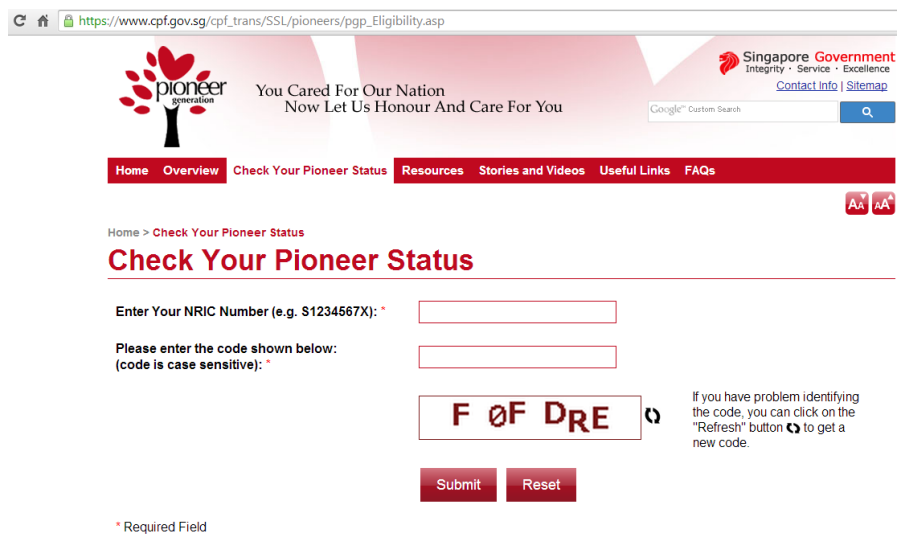
\includegraphics[width=0.65\paperwidth]{C:/Users/Admin/Desktop/Github/question_bank/LyX/static/img/9597-DHS-2014-P1-Q1}
\par\end{center}

A normalised database solution is to be designed, which has a number
of tables.
\begin{enumerate}
\item Derive the normalised process from the unnormalised form (UNF) to
the third normal form (3NF). \hfill{}{[}7{]}
\item Draw an ER diagram that shows these tables and the relationships between
them. \hfill{}{[}3{]}
\item Using suitable examples, explain the concepts of 
\begin{enumerate}
\item primary key \hfill{}{[}1{]}
\item foreign key \hfill{}{[}2{]}
\item composite key \hfill{}{[}2{]}
\end{enumerate}
\end{enumerate}

 \newpage 

\item \textbf{{[}DHS/PRELIM/9597/2014/P2/Q3{]} }

To enhance the security of online transactions, a one-time randomly
generated 5-digit Personal Identification Number (PIN) will be sent
to the user's registered mobile phone number as part of the authentication
process. The security algorithm, \texttt{Secret()}, makes use of the
sum of squares of the prime factors of the rightmost 5 digits of the
user's mobile number modulo $k$, where $k$ is a randomly generated
prime in the range 100000 -- 999999. 

As an illustration, consider the mobile phone number 87654321 ($n=54321$):

Sum of squares of prime factors of $n=3^{2}+19^{2}+953^{2}=908579$

PIN = 908579 modulo $k$ (let's say $k=102077$) = 91963 

So a one-time 5-digit PIN 91963 will be sent to the mobile number
87654321. 

The algorithm for finding the prime factors of a number n is detailed
recursively as follows: 
\begin{itemize}
\item If $n$ is even, one factor is 2, then find the prime factors of n/2. 
\item If $n$ is divisible by 3, remove this factor and then find the prime
factors of the remainder. 
\item If $n$ is divisible by 5, remove this factor and then find the prime
factors of the remainder. 
\item If $n$ is divisible by 7, remove this factor and then find the prime
factors of the remainder. 
\item ...
\end{itemize}
You may assume the availability of a random function \texttt{Random()}
but should indicate how it is used. 
\begin{enumerate}
\item Identify, giving examples, any pitfall(s) with your \texttt{Secret()}
algorithm, and suggest possible solution(s) to overcome them. \hfill{}{[}4{]}
\item Devise, incorporating your answer to (a), an efficient means of generating
a PIN using \texttt{Secret()}. Your function should include a recursive
algorithm for finding the prime factors of n. State explicitly any
necessary assumption(s) made. \hfill{}{[}6{]}
\end{enumerate}

 \newpage 

\item \textbf{{[}DHS/PRELIM/9597/2014/P2/Q4{]} }

Leveraging on technology, PGJC intends to connect all pioneers using
a social network to help foster a greater sense of community, promote
active aging and bridge the digital divide. 
\begin{enumerate}
\item What is a social network? Suggest two appropriate applications in
this context compared to traditional face-to-face interaction and
online communication means such as email and instant messaging.\hfill{}
{[}3{]} 
\item Give two benefits and one concern of hosting the social network using
cloud computing.\hfill{} {[}3{]}
\item Using appropriate examples, explain why the Object-Oriented Programming
(OOP) paradigm is well suited to implement the features of a social
network. \hfill{}{[}4{]}
\end{enumerate}

 \newpage 

\item \textbf{{[}DHS/PRELIM/9597/2014/P2/Q5{]} }

Pioneers who are eligible for the PGP must meet the following conditions: 
\begin{itemize}
\item still alive 
\item Aged 16 and above in 1965 
\item obtained citizenship on or before 31 December 1986 
\end{itemize}
Eligible pioneers enjoy the following benefits: 
\begin{itemize}
\item additional outpatient care subsidies 
\item Medisave account top-ups 
\item Medishield Life insurance subsidies and top-ups 
\end{itemize}
A panel will assess appeals for individuals who may have marginally
missed out on the PGP on a case-by-case basis. Citizens aged 55 and
above this year who do not qualify for the PGP will receive Medisave
account quantum top-ups for five years. 
\begin{enumerate}
\item Create a decision table showing all the possible conditions and actions.
\hfill{}{[}3{]}
\item Simplify your decision table by removing redundancies. \hfill{}{[}2{]}
\item Draw a program flowchart to determine if an individual is eligible
for the PGP and if not, if they qualify for an appeal or will receive
five-year quantum top-ups. \hfill{}{[}4{]}
\item Give 3 examples of test cases to test the age criteria for your algorithm
in (c). \hfill{}{[}3{]}
\item Given the date of birth in DD/MM/YYYY, write pseudocode to determine
if an individual is aged 16 and above in 1965. \hfill{}{[}3{]}
\end{enumerate}

 \newpage 

\item \textbf{{[}DHS/PRELIM/9597/2014/P2/Q6{]} }

While English is the official working language in Singapore, beneficiaries
of the PGP are elderly and a significant segment of them do not speak
or understand English. As a multi-racial society, the pioneer generation
also consists of Chinese, Malays and Indians. 
\begin{enumerate}
\item What is Unicode and why is it an appropriate representation for PGP
information compared to ASCII? \hfill{}{[}3{]}
\item Give two disadvantages of using Unicode in this context. \hfill{}
{[}2{]}
\end{enumerate}
Mailing information of the pioneers is currently held in a sequential
file in NRIC order: 
\noindent \begin{center}
\texttt{<NRIC><Statutory name><Address line><Postal code> }
\par\end{center}

Postal code is a 6-digit string representing the geographic location
of an address. To mail the PGP information to the pioneers efficiently,
three methods are proposed: 
\begin{itemize}
\item M1 - Sort the contents of the sequential file using quick sort on
the postal code field. 
\item M2 - Reorganise the contents of the sequential file to a linked list
of linked lists in ascending postal code order. Each node of the linked
list points to a linked list of addresses with the same postal code. 
\item M3 - Reorganize the contents of the sequential file to a binary search
tree using postal code as the key field. Each node in the binary search
tree points to a linked list of addresses with the same postal code. 
\end{itemize}
\begin{enumerate}
\item[(c)]  Why is quick sort appropriate or inappropriate for method M1? \hfill{}{[}3{]}
\item[(d)]  Draw diagrams to represent the scenario in 
\begin{enumerate}
\item method M2 using linked list 
\item method M3 using binary tree 
\end{enumerate}
Your diagrams should contain at least 3 nodes for each scenario. \hfill{}
{[}4{]}
\item[(e)]  Write an algorithm to insert a new entry to the linked list in method
M2, assuming a successful appeal. \hfill{} {[}4{]}
\item[(f)]  Write an algorithm to delete an entry from the binary search tree
in method M3, assuming the demise of a pioneer. \hfill{}{[}4{]}
\end{enumerate}

 \newpage 

\item \textbf{{[}HCI/PRELIM/9597/2014/P1/Q1{]} }

A program is to process daily high scores recorded from an online
game. The program can be run every day. 

All scores are integers in the range 1 to 500.

The program reads from file \texttt{HIGHEST.txt} the current highest
score and player name from running the program on previous days. 

The program specification is to: 
\begin{itemize}
\item input up to 5 player names and their corresponding scores for today 
\item calculate and display on screen: 
\begin{itemize}
\item the highest score with the player name for today 
\item a message saying whether or not the highest score today beat the current
highest score 
\end{itemize}
\item update the file \texttt{HIGHEST.txt} if a higher score was input today. 
\end{itemize}

\subsection*{Task 1.1 }

Write program code for this task. 

\subsection*{Evidence 1: }

Your program code. \hfill{}{[}7{]}

\subsection*{Task 1.2 }

Draw up a set of test data which tests the functioning of your program.
Consider carefully all cases which could occur for both the scores
input and the two processing requirements. 

\subsection*{Evidence 2: }

A screenshot for each test case you considered. Annotate the screenshot
explaining the purpose of each test. \hfill{}{[}8{]}

A \textbf{\emph{palindrome}} is an integer that reads the same backwards
and forwards -{}- so 6, 11 and 121 are all palindromes, while 10,
12, 223 and 2244 are not (even though 010=10, we don't consider leading
zeroes when determining whether a number is a palindrome). 

\subsection*{Task 1.3 }

Write program code with the following specification: 
\begin{itemize}
\item input two integers -{}- the endpoints of an interval e.g. \texttt{10
120 }
\item output the number of integers that are palindromes in the interval. 
\end{itemize}

\subsection*{Evidence 3: }

Your program code. \hfill{}{[}8{]}

\subsection*{Evidence 4: }

Produce two screenshots showing the output of 1 4 and 10 120 by the
user.\hfill{} {[}2{]}

 \newpage 

\item \textbf{{[}HCI/PRELIM/9597/2014/P1/Q2{]} }

The following is a pseudocode algorithm for the quick sort function. 

The function takes in an array and returns a sorted array in \textbf{ascending}
order. The algorithm works for most input but is missing out on a
few edge cases. 

\noindent %
\noindent\begin{minipage}[t]{1\columnwidth}%
\texttt{FUNCTION quicksort(array) }

\texttt{\qquad{}if array length = 1 }

\texttt{\qquad{}\qquad{}return array }

\texttt{\qquad{}select and remove a pivot value from array }

\texttt{\qquad{}create empty subarrays less and greater }

\texttt{\qquad{}for each item in array}

\texttt{\qquad{}\qquad{}if item < pivot }

\texttt{\qquad{}\qquad{}\qquad{}append item to less }

\texttt{\qquad{}\qquad{}else }

\texttt{\qquad{}\qquad{}\qquad{}append item to greater}

\texttt{\qquad{}return quicksort(less) + pivot + quicksort(greater) }%
\end{minipage}

\subsection*{Task 2.1 }

Write program code for this algorithm including all the amendments
you would make to: 
\begin{itemize}
\item make the function work for all cases 
\item adhere to good programming style 
\end{itemize}
Use the \texttt{Team} array sample data available from text file \texttt{SPORT+NAME+TEAM.txt}
and paste this into your program code.

\subsection*{Evidence 5: }

Your program code.\hfill{} {[}6{]}

\subsection*{Evidence 6: }

One screenshot showing the output from running the program code for
array Team.\hfill{} {[}1{]}

The following is a pseudocode algorithm of a binary search written
by a student to search for an item in an array Sport. This array stores
string data arranged in ascending order and has a final subscript
MAX. 

The algorithm is poorly designed and also contains errors. 

\noindent %
\noindent\begin{minipage}[t]{1\columnwidth}%
\texttt{Enter k }

\texttt{A = 1 }

\texttt{B = MAX }

\texttt{While not found }

\texttt{\qquad{}C = (A+B) DIV 2 }

\texttt{\qquad{}If Sport(C) = k }

\texttt{\qquad{}\qquad{}Print \textquotedblleft Found\textquotedblright{} }

\texttt{\qquad{}Else If Sport(C) < k }

\texttt{\qquad{}\qquad{}B = C-1 }

\texttt{\qquad{}Else }

\texttt{\qquad{}\qquad{}A = C+1 }

\texttt{\qquad{}End-If-Else }

\texttt{End-While }%
\end{minipage}

\subsection*{Task 2.2 }

Write program code for this algorithm including all the changes you
would make to: 
\begin{itemize}
\item follow good programming practice 
\item make the algorithm work properly 
\end{itemize}
Use the sample array data available from text file \texttt{SPORT+NAME+TEAM.txt}
and paste this into your programming code. 

\subsection*{Evidence 7: }

Your program code. \hfill{}{[}7{]}

\subsection*{Task 2.3 }

The binary search code could be useful for many programs where a search
routine is required. 

Re-design the program code to have a procedure \texttt{BinarySearch}.
This procedure should have parameters which allow it to be used for
\uline{any} sorted array of string data. 

Use the data provided in the array \texttt{Name} from text file \texttt{SPORT+NAME+TEAM.txt}
and test the procedure with appropriate test cases to ensure it is
working properly. 

\subsection*{Evidence 8: }

Your amended program code. \hfill{}{[}3{]}

\subsection*{Evidence 9: }

A screenshot for each appropriate test case. \hfill{}{[}3{]}

 \newpage 

\item \textbf{{[}HCI/PRELIM/9597/2014/P1/Q3{]} }

Morse Code is a type of code in which letters are represented by combinations
by long or short signals, e.g. the letter \textquoteleft A\textquoteright{}
is represented by a short followed by a long signal, i.e. \textquoteleft .-\textquoteleft{} 

Here we use the period (\textquoteleft .\textquoteright ) to represent
the short signal and the dash (\textquoteleft -\textquoteleft ) to
present the long signal. The Morse code equivalent for the letters
\textquoteleft A\textquoteright{} to \textquoteleft Z\textquoteright{}
is provided in the file \texttt{MORSE.txt}. In this implementation,
we use a space (\textquoteleft{} \textquoteleft ) to simulate the
inter-character gap and the slash (\textquoteleft /\textquoteright )
to represent the inter-word gap. 

\subsection*{Task 3.1 }

Write the program code for a function that will convert a given word
into its Morse Code equivalent using the following specification. 
\noindent \begin{center}
\texttt{FUNCTION ConvertWord(SingleWord : STRING): STRING }
\par\end{center}

The function has a single parameter \texttt{SingleWord} and returns
the Morse Code equivalent for that word as a string. 

\subsection*{Evidence 10: }

Your \texttt{ConvertWord} program code. \hfill{} {[}7{]}

\subsection*{Evidence 11: }

A screenshot showing the correct Morse Code equivalent for the word
\textquotedblleft COMPUTING\textquotedblright . \hfill{} {[}1{]}

\subsection*{Task 3.2 }

Write the program code that does the following: 
\begin{itemize}
\item the user inputs a sentence of words not exceeding 5 words. 
\item uses the function \texttt{ConvertWord} in Task 3.1 
\item outputs the Morse Code equivalent of the sentence of words that was
entered. 
\end{itemize}

\subsection*{Evidence 12: }

Your program code. \hfill{} {[}6{]}

\subsection*{Task 3.3}

Draw up \textbf{two} suitable tests to assess that your program is
working properly, explaining the reason for each test and provide
screenshot evidence for your testing. 

\subsection*{Evidence 13: }

Annotated screenshots for each test data run. \hfill{} {[}4{]}

\subsection*{Task 3.4 }

Write the program code that will do the following: the user enters
a word string in Morse Code the program converts the Morse Code word
to its alphabetical equivalent outputs the converted word.

\subsection*{Evidence 14: }

Your program code. \hfill{}{[}6{]}

\subsection*{Evidence 15: }

A screenshot showing the correct word equivalent for the following
Morse Code string, \textquotedblleft \dots{} \texttt{-{}-{}-} \dots \textquotedblright{}
\hfill{}{[}1{]}

 \newpage 

\item \textbf{{[}HCI/PRELIM/9597/2014/P1/Q4{]} }

Many programming languages use a variety of brackets eg \texttt{()},
\texttt{\{\}} and \texttt{{[}{]}} in their program statement constructs.
Brackets can be nested e.g. (()) and \{{[}{]}\}. A well-formed construct
must contain a matched set of optionally nested brackets e.g.\texttt{ (())},
\texttt{\{{[}{]}\}} and \texttt{()\{\}{[}{]}} are well-formed whereas\texttt{
(()},\texttt{ \{{]} }and\texttt{ )( }are not. 

An efficient way to check if a program construct is well-formed is
to use a stack to scan the brackets once from left to right as follows: 

Start from an empty stack. Whenever we encounter an open bracket,
push it into the stack. Whenever we encounter a close bracket, we
check if it is of the same type with the item at the top of the stack.
Once we have a match, we pop the topmost bracket from the stack. Only
when we managed to read the last bracket and find that the stack is
empty, then we know that the brackets are properly nested, and the
program construct is well-formed. 

The stack ADT contains character data and a top pointer, and has the
following operations: 
\begin{itemize}
\item \texttt{Create()} : initializes a new stack 
\item \texttt{Push(item)} : add item to top of stack 
\item \texttt{Pop()} : remove item from top of stack 
\item \texttt{Peep()} : inspect the topmost item of stack 
\item \texttt{isEmpty()} : check if stack is empty 
\end{itemize}

\subsection*{Task 4.1 }

Using object-oriented programming techniques, implement the stack
ADT using the class name \texttt{Stack}. 

\subsection*{Evidence 16: }

Your \texttt{Stack} class program code. \hfill{}{[}8{]}

\subsection*{Task 4.2 }

Write a function \texttt{CheckNested(construct)} which accepts a string
program construct of nested brackets and returns a Boolean result
indicating if construct is well-formed. 

\subsection*{Evidence 17: }

Your \texttt{CheckNested} function code. \hfill{}{[}10{]}

\subsection*{Task 4.3}

Test your \texttt{CheckNested} function using the data file provided
in \texttt{DATA.txt}. If a construct is not well-formed, append it
to a text file \texttt{ERRORS.txt}. 

\subsection*{Evidence 18: }

Screenshot of \texttt{ERRORS.txt}. \hfill{}{[}1{]}

\subsection*{Task 4.4}

Write a function \texttt{CheckWellformed(construct)} which contains
a modified and enhanced version of \texttt{CheckNested(construct)}.
When a first mismatch of bracket occurs, output the diagnostic message
\texttt{\textquotedbl Expecting '?'\textquotedbl}, where ? is the
type of bracket expected. For example, for the construct \texttt{())},
output the diagnostic message \texttt{\textquotedbl Expecting '('\textquotedbl}. 

\subsection*{Evidence 19: }

Your \texttt{CheckWellformed} function code. \hfill{}{[}10{]}

\subsection*{Task 4.5}

Test your \texttt{CheckWellformed} function using \texttt{ERRORS.txt}.
Display the diagnostic messages to screen.

\subsection*{Evidence 20: }

Screenshot of diagnostic messages on screen. \hfill{}{[}1{]}

 \newpage 

\item \textbf{{[}HCI/PRELIM/9597/2014/P2/Q1{]} }

Hwa Chong has partnered with Q\&M to set up a dental clinic in the
Campus. The clinic will have a few dentists to serve the student population.
The clinic will also have an on-line system for students to make appointment
with dentist. You are task to design the on-line system to handle
all student appointments. 
\begin{enumerate}
\item Draw an entity-relationship diagram for the appointment system. \hfill{}{[}7{]}
\item Convert the entity-relationship diagram into a relational database
schema. You may use shorthand notation to put across your answers.
Be certain to indicate the key fields. Your solution should include
a brief description for each table. \hfill{}{[}9{]}
\item Ensuring data integrity and security is an important issue in data
design. Explain why they are important for HC Dental system. \hfill{}{[}2{]}
\item The school plans to extent the dental service to other users after
the first year. Modify the entity relationship diagram to cater to
the teachers and staff too. \hfill{}{[}3{]}

Besides the data design, the user interface is an important factor
in determining the success of the HC dental system. The graphical
user interface for students to make an appointment using their desktops/laptops
must be intuitive and usable. 
\item Describe 3 design principles that will guide you in designing your
interfaces. Give specific examples on how you will incorporate it
into your user interface design for the HC dental system. \hfill{}{[}6{]}
\item Design the user-interfaces for the following features 
\begin{enumerate}
\item On-line appointment booking \hfill{}{[}3{]}
\item Updating of students particulars \hfill{}{[}3{]}
\end{enumerate}
\item Part of the future enhancement of the system is to allow a multimodal
interaction between the user and the system. A multimodal human-computer
interaction usually involves the 5 human senses and enables a more
free and natural communication. Suggest 2 realistic possibilities
for such an enhancement. Your suggestions should include a brief description
of how it works in this context.\hfill{}{[}4{]}

HC Dental system will reside in the school server and will allow access
beyond the school intranet. Mr Huang, the network administrator has
allocated an IP address 192.168.123.132 with a subnet mask 255.255.0.0
to access this system. 
\item Explain the following terms: 
\begin{enumerate}
\item IP address \hfill{}{[}1{]}
\item Subnet mask \hfill{}{[}1{]}
\end{enumerate}
\item Based on the information given, what is the network address? Show
the workings. \hfill{}{[}2{]}

The management team is concern with the accuracy of data transmitted/received
outside the school network. To ensure the team that they have looked
into this area, the development team highlighted that they have use
parity checks and checksums in detecting errors 
\item Explain parity checks and give an example to illustrate how it works.
\hfill{}{[}2{]}

The network administrator highlighted that there are proxy and firewalls
settings for devices accessing the school network. 
\item What is the purpose of a proxy server in the Network? \hfill{}{[}2{]}
\end{enumerate}

 \newpage 

\item \textbf{{[}HCI/PRELIM/9597/2014/P2/Q2{]} }
\begin{enumerate}
\item The Retail Company has engaged a software house to computerize its
operations. The project has been defined to contain the following
list of activities along with their required times for completion:
\noindent \begin{center}
\begin{tabular}{|c|l|c|c|}
\hline 
Activity & Description & Duration (Working Days) & Predecessor/s\tabularnewline
\hline 
\hline 
A & Requirement Analysis & 1 & \tabularnewline
\hline 
B & Systems Design & 3 & A\tabularnewline
\hline 
C & Programming & 5 & B\tabularnewline
\hline 
D & telecoms & 3 & B\tabularnewline
\hline 
E & Hardware Installation & 6 & B\tabularnewline
\hline 
F & Integration & 2 & C, D\tabularnewline
\hline 
G & System Testing & 2 & E, F\tabularnewline
\hline 
H & Training/Support & 1 & G\tabularnewline
\hline 
I & Handover and Go-Live & 1 & H\tabularnewline
\hline 
\end{tabular}
\par\end{center}
\begin{enumerate}
\item Complete the PERT chart below, indicating the earliest start time
and latest start time of each activity: 
\end{enumerate}
\begin{center}
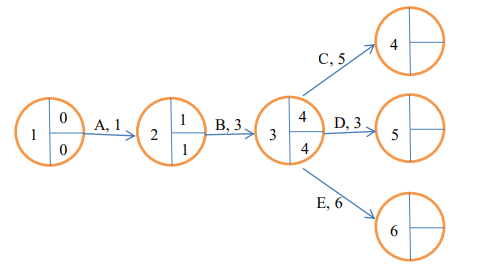
\includegraphics[width=0.65\paperwidth]{C:/Users/Admin/Desktop/Github/question_bank/LyX/static/img/9597-HCI-2014-P1-Q2}
\par\end{center}

\hfill{}{[}4{]}
\begin{enumerate}
\item State the critical path. \hfill{}{[}1{]}
\item State the elapsed time of the project. \hfill{}{[}1{]}
\item State 2 activities not on the critical path, as well as their slack
time. \hfill{}{[}2{]}
\end{enumerate}
\item The Gantt chart below is based on the above information. There are
three activities missing and three activities shown are incorrect.
Draw a sketch of the Gantt chart to show the correct version. 
\noindent \begin{center}
\begin{tabular}{c|c|c|c|c|c|c|c|c|c|c|c|c|c|c|c|c|c|c|c|}
\multicolumn{20}{c}{Weeks}\tabularnewline
\multicolumn{1}{c}{Activity} & \multicolumn{1}{c}{1} & \multicolumn{1}{c}{2} & \multicolumn{1}{c}{3} & \multicolumn{1}{c}{4} & \multicolumn{1}{c}{5} & \multicolumn{1}{c}{6} & \multicolumn{1}{c}{7} & \multicolumn{1}{c}{8} & \multicolumn{1}{c}{10} & \multicolumn{1}{c}{11} & \multicolumn{1}{c}{12} & \multicolumn{1}{c}{13} & \multicolumn{1}{c}{14} & \multicolumn{1}{c}{15} & \multicolumn{1}{c}{16} & \multicolumn{1}{c}{17} & \multicolumn{1}{c}{18} & \multicolumn{1}{c}{19} & \multicolumn{1}{c}{20}\tabularnewline
\cline{2-20} \cline{3-20} \cline{4-20} \cline{5-20} \cline{6-20} \cline{7-20} \cline{8-20} \cline{9-20} \cline{10-20} \cline{11-20} \cline{12-20} \cline{13-20} \cline{14-20} \cline{15-20} \cline{16-20} \cline{17-20} \cline{18-20} \cline{19-20} \cline{20-20} 
A & X &  &  &  &  &  &  &  &  &  &  &  &  &  &  &  &  &  & \tabularnewline
\cline{2-20} \cline{3-20} \cline{4-20} \cline{5-20} \cline{6-20} \cline{7-20} \cline{8-20} \cline{9-20} \cline{10-20} \cline{11-20} \cline{12-20} \cline{13-20} \cline{14-20} \cline{15-20} \cline{16-20} \cline{17-20} \cline{18-20} \cline{19-20} \cline{20-20} 
B &  & X & X & X &  &  &  &  &  &  &  &  &  &  &  &  &  &  & \tabularnewline
\cline{2-20} \cline{3-20} \cline{4-20} \cline{5-20} \cline{6-20} \cline{7-20} \cline{8-20} \cline{9-20} \cline{10-20} \cline{11-20} \cline{12-20} \cline{13-20} \cline{14-20} \cline{15-20} \cline{16-20} \cline{17-20} \cline{18-20} \cline{19-20} \cline{20-20} 
C &  &  &  &  &  & X & X & X & X & X &  &  &  &  &  &  &  &  & \tabularnewline
\cline{2-20} \cline{3-20} \cline{4-20} \cline{5-20} \cline{6-20} \cline{7-20} \cline{8-20} \cline{9-20} \cline{10-20} \cline{11-20} \cline{12-20} \cline{13-20} \cline{14-20} \cline{15-20} \cline{16-20} \cline{17-20} \cline{18-20} \cline{19-20} \cline{20-20} 
D &  &  &  &  &  &  &  & X & X & X &  &  &  &  &  &  &  &  & \tabularnewline
\cline{2-20} \cline{3-20} \cline{4-20} \cline{5-20} \cline{6-20} \cline{7-20} \cline{8-20} \cline{9-20} \cline{10-20} \cline{11-20} \cline{12-20} \cline{13-20} \cline{14-20} \cline{15-20} \cline{16-20} \cline{17-20} \cline{18-20} \cline{19-20} \cline{20-20} 
E &  &  &  &  & X & X & X & X & X & X &  &  &  &  &  &  &  &  & \tabularnewline
\cline{2-20} \cline{3-20} \cline{4-20} \cline{5-20} \cline{6-20} \cline{7-20} \cline{8-20} \cline{9-20} \cline{10-20} \cline{11-20} \cline{12-20} \cline{13-20} \cline{14-20} \cline{15-20} \cline{16-20} \cline{17-20} \cline{18-20} \cline{19-20} \cline{20-20} 
F &  &  &  &  &  &  &  &  &  &  & X & X &  &  &  &  &  &  & \tabularnewline
\cline{2-20} \cline{3-20} \cline{4-20} \cline{5-20} \cline{6-20} \cline{7-20} \cline{8-20} \cline{9-20} \cline{10-20} \cline{11-20} \cline{12-20} \cline{13-20} \cline{14-20} \cline{15-20} \cline{16-20} \cline{17-20} \cline{18-20} \cline{19-20} \cline{20-20} 
G &  &  &  &  &  &  &  &  &  &  &  &  &  &  &  &  &  &  & \tabularnewline
\cline{2-20} \cline{3-20} \cline{4-20} \cline{5-20} \cline{6-20} \cline{7-20} \cline{8-20} \cline{9-20} \cline{10-20} \cline{11-20} \cline{12-20} \cline{13-20} \cline{14-20} \cline{15-20} \cline{16-20} \cline{17-20} \cline{18-20} \cline{19-20} \cline{20-20} 
H &  &  &  &  &  &  &  &  &  &  &  &  &  &  &  &  &  &  & \tabularnewline
\cline{2-20} \cline{3-20} \cline{4-20} \cline{5-20} \cline{6-20} \cline{7-20} \cline{8-20} \cline{9-20} \cline{10-20} \cline{11-20} \cline{12-20} \cline{13-20} \cline{14-20} \cline{15-20} \cline{16-20} \cline{17-20} \cline{18-20} \cline{19-20} \cline{20-20} 
I &  &  &  &  &  &  &  &  &  &  &  &  &  &  &  &  &  &  & \tabularnewline
\cline{2-20} \cline{3-20} \cline{4-20} \cline{5-20} \cline{6-20} \cline{7-20} \cline{8-20} \cline{9-20} \cline{10-20} \cline{11-20} \cline{12-20} \cline{13-20} \cline{14-20} \cline{15-20} \cline{16-20} \cline{17-20} \cline{18-20} \cline{19-20} \cline{20-20} 
\end{tabular}
\par\end{center}

\end{enumerate}

 \newpage 

\item \textbf{{[}HCI/PRELIM/9597/2014/P2/Q3{]} }

All\textquoteright s Well Hospital is in the process of computerizing
its clinic processes. At the clinic, there are various doctors specializing
in different areas e.g. neuroscience specialists, gynaecologists,
etc. All patients of the clinic must be registered in the patient
database and make prior appointments to see the relevant doctors.
No walk-in patients will be entertained. Appointments are made based
on the doctor\textquoteright s weekly schedule i.e. different doctors
have clinic sessions at different day/time of the week. 

On the day of appointment, patients are to register at the self-registration
counter before proceeding to the doctor\textquoteright s room. Upon
seeing the doctor, the doctor will input the diagnosis into the system.
After the doctor\textquoteright s consultation, the patient is to
proceed to make payment. Upon payment, a prescription slip, reference
letter, medical certificate, will be printed as necessary for the
patient. In addition, the next appointment may be scheduled, if necessary. 
\begin{enumerate}
\item Use a diagram to show the data flows, processes, data stores and external
links in the system. \hfill{}{[}10{]}
\item At the self-registration counter, patients can scan the barcode of
their appointment card or NRIC. Alternatively, they can also enter
their NRIC number using the keyboard. When the NRIC is entered using
the keyboard, it must be validated and verified. 
\begin{enumerate}
\item Explain the difference between validation and verification of data.
\hfill{}{[}2{]}
\item Describe two validation tests that can be performed on the NRIC number
entered. \hfill{}{[}2{]}
\item Describe how the NRIC number entered by the patient can be verified
by the system.\hfill{}{[}1{]}
\end{enumerate}
\item As part of the hospital welfare program, there is a fitness center
for staff. To enter the fitness center, staff needs to use a swipe
card together with a 4-digit PIN to gain access. Access is only allowed
if there are fewer than 50 people already in the fitness center, in
order to avoid overcrowding. Access is also restricted to one person
per card. If maintenance is being carried out then access is denied
and a message is output to a screen asking the staff to return in
1 hour. In order to exit the fitness center, the swipe card is used
again. Using appropriate variable names, write in pseudocode, an algorithm
to control the entry system to the fitness center.\hfill{}{[}8{]}
\end{enumerate}

 \newpage 

\item \textbf{{[}HCI/PRELIM/9597/2014/P2/Q4{]} }

A Retail Company has a customer loyalty program that gives a range
of discounts. For customers in the loyalty program between 5 to 9
years, they will receive a 5\% discount. For 10 or more years, the
customer will receive a 10\% discount. However, whether a customer
is in the loyalty program or not, if the cumulative value of his purchases
for this calendar year exceed \$1000, he will receive a 15\% discount.
Note: Aggregation of discounts is not allowed. 
\begin{enumerate}
\item Create a decision table that shows all possible outcomes for the above
loyalty program. 
\item Draw the decision table after redundancies have been removed. \hfill{}{[}6{]}
\item Using your answer in (b), write a function using pseudocode. The function
returns: 
\begin{itemize}
\item 0 to indicate no discount 
\item the percentage discount offered\hfill{}{[}4{]}
\end{itemize}
\end{enumerate}

 \newpage 

\item \textbf{{[}HCI/PRELIM/9597/2014/P2/Q5{]} }

An apartment block in a city consists of a large number of apartments.
Each of the residents of the apartments has their information stored
in a file. 

The records in the file are to be sorted into alphabetical order of
the resident\textquoteright s name. 
\begin{enumerate}
\item Using the following list of names as an example, show how the records
can be sorted into alphabetical order using an insertion sort. 
\noindent \begin{center}
GRA, CHR, DAV, SAR, TOM, KAT \hfill{}{[}4{]}
\par\end{center}
\item Residents sometimes make requests for maintenance on their apartments.
Each request is given a priority number ranging from 1, for failure
of the air conditioning, to 10, for a dripping tap. Each request is
stored in a linked list in order of priorities. Jobs with equal priority
are stored in order of the date that they have been submitted. 

Describe an algorithm to insert a new job into the list. \hfill{}{[}6{]}
\end{enumerate}

 \newpage 

\item \textbf{{[}PJC/PRELIM/9597/2014/P1/Q1{]} }

At the Commonwealth Games, the timings for the heats of 100m race
are recorded in a file \texttt{RACE.csv}. 

Each record has the following format: 
\noindent \begin{center}
\texttt{<runnerID>,<country code>,<name of runner>,<race time> }
\par\end{center}

A sample record is: 
\noindent \begin{center}
\texttt{2225,SIN,Kang,10.77} 
\par\end{center}

\subsection*{Task 1.1 }

Write program code to find and output the \textbf{\emph{number of
runners}} who recorded a timing of more than 11 seconds, and \textbf{\emph{list
these runners}} on the screen along with their full records under
this heading: 
\noindent \begin{center}
\texttt{}%
\begin{tabular}{|cccc|}
\hline 
\texttt{Runner ID } & \texttt{Country} & \texttt{Name } & \texttt{Race Time}\tabularnewline
\hline 
\end{tabular}
\par\end{center}

\subsection*{Evidence 1: }

Your program code for task 1.1. \hfill{}{[}6{]}

\subsection*{Evidence 2: }

Screenshot of output. \hfill{}{[}1{]}

\subsection*{Task 1.2 }

Write program code to display the top 10 runners in order of race
time. Runners with the same race time will have the same rank. The
fastest runner will be displayed first, under this heading: Runner
ID 
\noindent \begin{center}
\texttt{}%
\begin{tabular}{|cccc|}
\hline 
\texttt{Runner ID} & \texttt{Country} & \texttt{Name} & \texttt{Race Time}\tabularnewline
\hline 
\end{tabular}
\par\end{center}

\subsection*{Evidence 3: }

Your program code for task 1.2. \hfill{}{[}7{]}

\subsection*{Evidence 4: }

Screenshot of output. \hfill{}{[}1{]}

 \newpage 

\item \textbf{{[}PJC/PRELIM/9597/2014/P1/Q2{]} }

A pseudocode algorithm for a binary search on an array \texttt{CITY}
is shown below. This array stores records of city, and its country
and population. Array is sorted by name of city. It has an initial
subscript 1 and final subscript \texttt{MAX}. The algorithm can be
improved to make it clearer and more efficient. 

\noindent %
\noindent\begin{minipage}[t]{1\columnwidth}%
\texttt{Set element\_found to false }

\texttt{Set low\_element to 1 }

\texttt{Set high\_element to MAX }

\texttt{\textbf{DOWHILE}}\texttt{ (NOT element\_found)}

\texttt{\qquad{}index = (low\_element + high\_element)/2 }

\texttt{\qquad{}}\texttt{\textbf{IF}}\texttt{ CITY(index) = input\_value
}\texttt{\textbf{THEN}}\texttt{ }

\texttt{\qquad{}\qquad{}Set element\_found to true }

\texttt{\qquad{}}\texttt{\textbf{ELSE}}\texttt{ }

\texttt{\qquad{}\qquad{}}\texttt{\textbf{IF}}\texttt{ input\_value
<= CITY(index) }\texttt{\textbf{THEN}}\texttt{ }

\texttt{\qquad{}\qquad{}\qquad{}high\_element = index \textendash{}
1 }

\texttt{\qquad{}\qquad{}}\texttt{\textbf{ELSE}}\texttt{ }

\texttt{\qquad{}\qquad{}\qquad{}low\_element = index + 1 }

\texttt{\qquad{}\qquad{}}\texttt{\textbf{ENDIF}}

\texttt{\qquad{}}\texttt{\textbf{ENDIF}}\texttt{ }

\texttt{\textbf{ENDDO}}

\texttt{\textbf{IF}}\texttt{ element\_found = true }\texttt{\textbf{THEN}}\texttt{ }

\texttt{\qquad{}Print index}

\texttt{\textbf{ELSE}}\texttt{ }

\texttt{\qquad{}Print \textquotedbl sorry\textquotedbl{} }

\texttt{ENDIF }%
\end{minipage}

\subsection*{Task 2.1 }

Write program code for this algorithm and improve on clarity and efficiency.
Include the sample array data available by reading from the file \texttt{CITY.csv}.
If a city is found after searching, display the full record of the
city, which includes country and population. 

\subsection*{Evidence 5: }

Your program code. \hfill{} {[}6{]}

\subsection*{Evidence 6: }

Produce a screenshot of running your program code, by searching for
\texttt{\textbf{Istanbul}} and \texttt{\textbf{Aberdeen}}. \hfill{}
{[}2{]}

\subsection*{Task 2.2 }

Write the binary search algorithm as a recursive function. Using comment
lines, explain on your choice of parameters passed into the recursive
function and return value, if any. 

\subsection*{Evidence 7: }

Your program code. \hfill{} {[}7{]}

 \newpage 

\item \textbf{{[}PJC/PRELIM/9597/2014/P1/Q3{]} }

Implement a linked list to store names of runners and their best running
times in seconds, in ascending order of running time. The runner with
the fastest timing is stored at the first node while the runner with
the slowest timing is stored at the last node. A linked list of free
nodes is also implemented with a maximum size of 20 nodes. 

The program will use a user-defined type \texttt{Node} for each node
defined as follows: 
\begin{center}
\begin{tabular}{|l|l|l|}
\hline 
\texttt{\textbf{\hspace{0.01\columnwidth}}}\textbf{Identifier} & \texttt{\textbf{\hspace{0.01\columnwidth}}}\textbf{Data Type} & \texttt{\textbf{\hspace{0.05\columnwidth}}}\textbf{Description}\tabularnewline
\hline 
\texttt{Name} & \texttt{STRING} & The name of the runner\tabularnewline
\hline 
\texttt{Time} & \texttt{FLOAT} & The best running time of the runner\tabularnewline
\hline 
\texttt{Next} & \texttt{POINTER} & The pointer to the next node \tabularnewline
\hline 
\end{tabular}
\par\end{center}

The program will also use another user-defined type \texttt{LinkedList}
for each linked list. It contains a \texttt{first} pointer that points
to the first node of the linked list and makes use of \texttt{Node}
for its nodes. 

The user-defined type LinkedList contains methods as follows: 
\begin{center}
\begin{tabular}{|l|l|}
\hline 
\texttt{\textbf{\hspace{0.01\columnwidth}}}\textbf{Method} & \texttt{\textbf{\hspace{0.05\columnwidth}}}\textbf{Description}\tabularnewline
\hline 
\texttt{Display } & To display the contents of the linked list in order \tabularnewline
\hline 
\texttt{AddFirst } & To add a new node as first node of linked list\tabularnewline
\hline 
\texttt{RemoveFirst } & To remove first node of linked list\tabularnewline
\hline 
\texttt{AddLast} & To add a new node as last node of linked list \tabularnewline
\hline 
\texttt{RemoveLast} & To remove last node of linked list\tabularnewline
\hline 
\texttt{Empty} & To return Boolean True if linked list is empty\tabularnewline
\hline 
\end{tabular}
\par\end{center}

The diagram shows two linked lists -- \texttt{RaceList} and \texttt{FreeList}.

\texttt{RaceList} contains a dataset of four nodes. Each node contains
a \emph{name}, a \emph{running time}, and a \emph{pointer} to the
next node. 

\texttt{FreeList} is a list of free nodes available for \texttt{RaceList}
to store data, where the maximum number of nodes is 20.
\begin{center}
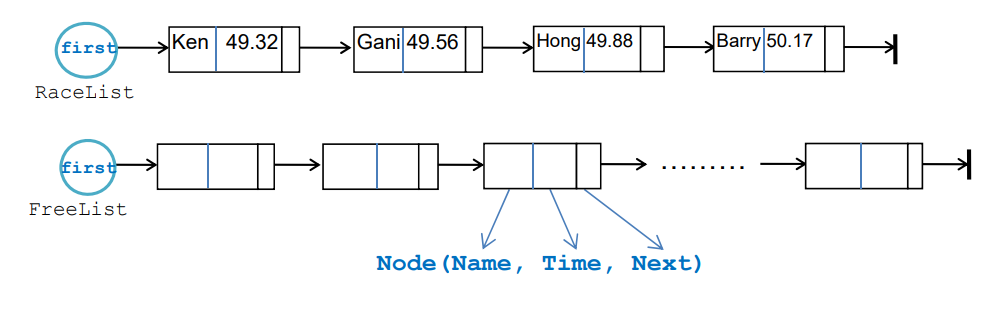
\includegraphics[width=0.65\paperwidth]{C:/Users/Admin/Desktop/Github/question_bank/LyX/static/img/9597-PJC-2014-P1-Q3}
\par\end{center}

\subsection*{Task 3.1 }

Write program code to create \texttt{Node} and \texttt{LinkedList},
and initialise an empty linked \texttt{RaceList}, and \texttt{FreeList}
of \textbf{20} nodes. Ensure all identifiers and methods specified
above are created. 

\subsection*{Evidence 8: }

Your program code for task 3.1. \hfill{}{[}17{]}

\subsection*{Evidence 9: }

Screenshot of running method to display \texttt{RaceList} and \texttt{FreeList}
on screen. \hfill{}{[}1{]}

\subsection*{Task 3.2 }

Write code to implement a method \texttt{AddInOrder} that will add
a new node with data into \texttt{RaceList} in ascending order of
running time. Node added to \texttt{RaceList} should be taken from
\texttt{FreeList}. 

\subsection*{Evidence 10: }

Your program code for task 3.2. \hfill{}{[}11{]}

\subsection*{Task 3.3 }

Test your program using the following data items input in the order
shown and run method to display \texttt{RaceList} and \texttt{FreeList}
on screen. 
\noindent \begin{center}
\begin{tabular}{|c|c|c|}
\hline 
\textbf{Order of input } & \textbf{Name} & \textbf{Running Time}\tabularnewline
\hline 
\hline 
1 & Barry & 50.17\tabularnewline
\hline 
2 & Gani  & 49.56\tabularnewline
\hline 
3 & Hong & 49.88\tabularnewline
\hline 
4 & Ken & 49.32 \tabularnewline
\hline 
\end{tabular} 
\par\end{center}

\subsection*{Evidence 11: }

Provide screenshot for task 3.3. \hfill{} {[}2{]}

\subsection*{Task 3.4 }

Write code to implement a method \texttt{RemoveNode} that will remove
the node that contains data specified by user to be removed from \texttt{RaceList}.
Node removed from \texttt{RaceList} should be returned to \texttt{FreeList}. 

\subsection*{Evidence 12: }

Your program code for task 3.4. \hfill{}{[}8{]}

\subsection*{Task 3.5 }

Test your program by removing \texttt{Gani} from \texttt{RaceList}
and run method to display \texttt{RaceL}ist and \texttt{FreeList}
on screen. 

\subsection*{Evidence 13: }

Provide screenshot for task 3.5. \hfill{} {[}1{]}

 \newpage 

\item \textbf{{[}PJC/PRELIM/9597/2014/P1/Q4{]} }

A message is encrypted and passed between two parties. To decrypt
the message, a \textquotedblleft key\textquotedblright{} is applied.
Both the sending and receiving parties hold the key which enables
them to encrypt and decrypt the message. 

An approach of cryptography is the simple substitution cipher, a method
of encryption by which each letter of a message is substituted with
another letter. The receiving party deciphers the text by performing
an inverse substitution. 

The substitution system is created by first writing out a \emph{phrase}.
The key is then derived from the phrase by removing all the repeated
letters. The \emph{cipher text} alphabet is then constructed starting
with the letters of the \emph{key} and then followed by all the remaining
letters in the alphabet. 

Using this system, the phrase \textquotedbl\texttt{apple}\textquotedbl{}
gives us the key as \textquotedbl\texttt{APLE}\textquotedbl{} and
the following substitution scheme: 

\begin{tabular}{cccccccccccccccccccccccccccc}
\textbf{Plain text alphabet :} & a & b & c & d & e & f & g & h & i & j & k & l & m & n & o & p & q & r & s & t & u & v & w & x & y & z & \tabularnewline
 & $\downarrow$ &  &  & $\downarrow$ & \multicolumn{21}{c}{$\cdots$$\cdots$$\cdots$$\cdots$$\cdots$$\cdots$$\cdots$$\cdots$} & $\downarrow$ & is substituted by\tabularnewline
\textbf{Cipher text alphabet :} & A & P & L & E & B & C & D & F & G & H & I & J & K & M & N & O & Q & R & S & T & U & V & W & X & Y & Z & \tabularnewline
\end{tabular}

\texttt{'a'} will be substituted by \texttt{'A'}, \texttt{'b'} will
be substituted by \texttt{'P'}, \texttt{'c'} will be substituted by
\texttt{'L'}, \texttt{'d'} will be substituted by\texttt{ 'E'},\texttt{
'e' }will be substituted by \texttt{'B'}, and so on. 

\subsection*{Task 4.1 }

Write program code for a function to create cipher text using the
following specification:
\noindent \begin{center}
\texttt{FUNCTION CreateCipher (phrase : STRING) : STRING }
\par\end{center}

The function \texttt{CreateCipher} has a single parameter \texttt{phrase}
and returns the cipher text alphabet as a string. 

\subsection*{Evidence 14: }

Your program code for task 4.1.\hfill{} {[}8{]}

\subsection*{Task 4.2 }

Write program code for a procedure \texttt{CreateCipherTest} which
does the following: 
\begin{itemize}
\item read the phrases from file phrases.txt 
\item create cipher text for each of the phrases 
\item display each phrase and cipher text on the screen as follows: 

\noindent\fbox{\begin{minipage}[t]{1\columnwidth - 2\fboxsep - 2\fboxrule}%
\texttt{Phrase: apple }

\texttt{Cipher text: APLEBCDFGHIJKMNOQRSTUVWXYZ }

\texttt{... ...}

\texttt{... ... }%
\end{minipage}}
\end{itemize}

\subsection*{Evidence 15: }

Your program code for task 4.2.\hfill{} {[}3{]}

\subsection*{Evidence 16: }

Screenshot for running task 4.2. \hfill{}{[}1{]}

\subsection*{Task 4.3}

Write program code for a function to decrypt a message using the following
specification: 
\noindent \begin{center}
\texttt{FUNCTION Decrypt (enc\_message:STRING, cipher:STRING) : STRING }
\par\end{center}

The function \texttt{Decrypt} accepts parameters \texttt{enc\_message}
and \texttt{cipher}, and returns the decrypted message as a string.
Parameter \texttt{enc\_message} is the encrypted message, and parameter
\texttt{cipher} is the cipher text alphabet. 

\subsection*{Evidence 17: }

Your program code for task 4.3. \hfill{}{[}6{]}

\subsection*{Task 4.4 }

Write program code which does the following: 
\begin{itemize}
\item read the phrase and encrypted message from file \texttt{cipher.txt }
\item cipher text is generated from \texttt{CreateCipher} function 
\item message is decrypted from \texttt{Decrypt} function 
\item display decrypted message on the screen together with the phrase and
encrypted message 

\noindent\fbox{\begin{minipage}[t]{1\columnwidth - 2\fboxsep - 2\fboxrule}%
\texttt{Phrase: ...}

\texttt{Encrypted message: ...}

\texttt{Decrypted message: ...}%
\end{minipage}}
\end{itemize}

\subsection*{Evidence 18: }

Your program code for task 4.4.\hfill{} {[}3{]}

\subsection*{Evidence 19: }

Screenshot for running task 4.4. \hfill{}{[}1{]}

\subsection*{Task 4.5 }

Write program code for a function to encrypt a message using the following
specification:

\texttt{FUNCTION Encrypt (message:STRING, cipher:STRING) : STRING}

The function \texttt{Encrypt} accepts parameters \texttt{message}
and \texttt{phrase}, and returns the encrypted message as a string.
Parameter \texttt{message} is the message to be encrypted while parameter
\texttt{cipher} is the cipher text. 

\subsection*{Evidence 20: }

Your program code for task 4.5.\hfill{} {[}4{]}

\subsection*{Task 4.6 }

Write program code which does the following: 
\begin{itemize}
\item encrypt the message: \textquotedblleft \texttt{do not give up!}\textquotedblright{}
\item use the phrase: \textquotedblleft \texttt{skyhigh}\textquotedblright{} 
\item generate cipher text from \texttt{CreateCipher} function
\item message is encrypted using \texttt{Encrypt} function
\item encrypted message is displayed on screen as follows: 

\noindent\fbox{\begin{minipage}[t]{1\columnwidth - 2\fboxsep - 2\fboxrule}%
\texttt{Phrase: skyhigh}

\texttt{Encrypted message: ...}%
\end{minipage}}
\end{itemize}

\subsection*{Evidence 21: }

Your program code for task 4.6. \hfill{}{[}3{]}

\subsection*{Evidence 22: }

Screenshot for running task 4.6. \hfill{}{[}1{]}

 \newpage 

\item \textbf{{[}PJC/PRELIM/9597/2014/P2/Q1{]} }

A manual system for producing school student reports works in the
following manner: 
\begin{itemize}
\item a subject report is completed for each subject that a student takes
by the single teacher teaching that subject; 
\item to help the subject teacher, initially a blank report form is issued
to the student for the student to add their details: student NRIC,
name, contact phone, teacher and class; 
\item the subject report is completed by the teacher with appropriate comments; 
\item all subject reports for the student are passed to the student's tutor; 
\item the tutor puts all the subject reports together to form the student's
report folder; 
\item the tutor adds a tutor's report including attendance data supplied
by the school administration attendance records; 
\item each student's report folder is copied; 
\item the copy is filed in the report storage facility for the school; 
\item the report folder is sent to the student's parents. 
\end{itemize}
The school has decided to replace this manual system with a computerised
system. 

A system developer is employed to carry out the task. The first task
assigned to the system developer is to write a project proposal.
\begin{enumerate}
\item One section of the project proposal is the Problem Statement which
lists the problems in the current system. Write the Problem Statement.\hfill{}
{[}4{]}
\item The proposal is accepted and the main stages of the project have been
identified and durations assessed as follows: 

\begin{tabular}{|c|l|c|l|}
\hline 
Stage & Description & Weeks & Staffing\tabularnewline
\hline 
\hline 
A & analysis of the solution & 4 & Analyst A1\tabularnewline
\hline 
B & design of the solution & 8 & Analysts A2 and A3 \tabularnewline
\hline 
C & development of the solution & 12 & Programmers P1 and P2\tabularnewline
\hline 
D & documentation of the solution & 8 & Clerks C1 and C2\tabularnewline
\hline 
E & implementation of the solution & 6 & Programmer P1\tabularnewline
\hline 
F & testing of the solution & 4 & Programmers P3 and P4\tabularnewline
\hline 
\end{tabular}

B and D cannot start until A is completed 

F and C cannot start until B is completed 

E cannot start until C is completed 

The project will end when D, E and F are completed.
\begin{enumerate}
\item Draw a Program Evaluation and Review Technique (PERT) chart for these
6 project stages (A to F). \hfill{}{[}4{]}
\item Calculate and display on the diagram, with a node layout key, the
earliest and latest start and finish times of each task. \hfill{}{[}4{]}
\item State the critical path.\hfill{} {[}1{]}
\item State the minimum time in which the project could be completed. \hfill{}{[}1{]}
\item Explain dependent stages and concurrent stages. For each type of stage
give an example from this chart. \hfill{}{[}4{]}
\item A decision is made that the PERT chart should show more detail with
regard to testing. It is proposed that stage F (testing) should be
removed from the chart and three new stages added:

L -- black box testing -- 2 weeks 

M -- white box testing -- 2 weeks

N -- beta testing -- 3 weeks 

Redraw the PERT chart to show the effect of these changes.\hfill{}
{[}2{]}
\item Draw a Gantt chart showing all \textbf{eight} stages and their dependencies,
allowing for the resource allocations as indicated above. \hfill{}{[}4{]}
\item List and explain briefly \textbf{TWO} advantages and \textbf{ONE}
disadvantage of using a Program Evaluation and Review Technique (PERT)
chart for a project plan in comparison with using a Gantt chart. \hfill{}{[}3{]}
\end{enumerate}
\item Identify \textbf{FIVE} key stages with brief description of the software
development life cycle (SDLC). \hfill{}{[}3{]}
\item At which stage of the SDLC is top-down analysis used? Explains why
it helps in the solution of complex problems. \hfill{}{[}2{]}
\item The attendance data enter into the new system needs to be validated
and verified. Explain with examples the difference between data validation
and data verification. \hfill{}{[}4{]}
\item Marek is designing a program for this computerised system. His test
strategy includes beta testing and acceptance testing.
\begin{enumerate}
\item Describe what is meant by beta testing and how it can be used to test
Marek\textquoteright s program. \hfill{} {[}2{]}
\item Describe what is meant by acceptance testing and how it can be used
to test Marek\textquoteright s program. \hfill{}{[}2{]}
\end{enumerate}
\item Teachers spend part of their week working from home. A system analyst
will assist in improving their school communication systems. Explain
why it is important to define problem accurately. {[}2{]} 
\item Subject teachers and tutors are worried because so much information
is being stored about their students on the server of the school.
Describe the fears that the teachers may have and explain what the
school can do to allay those fears. \hfill{}{[}3{]}
\item When data is transmitted between devices on a network it is liable
to corruption. One way of checking data for corruption is to carry
out a check sum. What is check sum? \hfill{}{[}1{]}
\item Explain another method of checking data to ensure that it has been
transmitted without corruption. \hfill{}{[}2{]}
\item When data is transmitted on a network it can use a number of different
transmission modes. State what is meant by each of the following modes
of data transmission.
\begin{enumerate}
\item Simplex \hfill{}{[}1{]}
\item Duplex \hfill{}{[}1{]}
\item Half-duplex \hfill{} {[}1{]}
\end{enumerate}
\end{enumerate}

 \newpage 

\item \textbf{{[}PJC/PRELIM/9597/2014/P2/Q2{]} }

A programmer is going to write part of the computer system, using
an object-oriented programming language, which will store details
subject teachers and tutors. All teachers and tutors will be identified
by their NRICs. 

Properties identified the subject teachers: 
\begin{itemize}
\item Subject code 
\end{itemize}
Properties identified the tutors: 
\begin{itemize}
\item Class name 
\end{itemize}
\begin{enumerate}
\item Draw a diagram that shows how the properties could be distributed
amongst a number of classes. Include in your diagram any inheritance
between classes. Also indicate some of the methods that would be required.
\hfill{}{[}4{]}
\item In the context of object-oriented programming explain what is meant
by:
\begin{enumerate}
\item encapsulation; \hfill{}{[}1{]}
\item inheritance;\hfill{} {[}1{]}
\item polymorphism. \hfill{}{[}1{]}
\end{enumerate}
\item Give two advantages of object-oriented programming. \hfill{}{[}2{]}
\end{enumerate}

 \newpage 

\item \textbf{{[}PJC/PRELIM/9597/2014/P2/Q3{]} }

The words COW, BEEF and FORTY have all their letters written in alphabetical
order. Here is an algorithm for a function which checks whether all
the letters in a word are in alphabetical order. 

\noindent\begin{minipage}[t]{1\columnwidth}%
\texttt{01 FUNCTION IsInOrder(Word) }

\texttt{02 \qquad{}IF LENGTH(Word) = 1 THEN }

\texttt{03 \qquad{}\qquad{}RETURN TRUE }

\texttt{04 \qquad{}ELSE }

\texttt{05 \qquad{}\qquad{}FirstChar = First character in Word }

\texttt{06 \qquad{}\qquad{}RestOfWord = All characters in Word except
the first }

\texttt{07 \qquad{}\qquad{}IF FirstChar > RestOfWord THEN }

\texttt{08 \qquad{}\qquad{}\qquad{}RETURN FALSE }

\texttt{09 \qquad{}\qquad{}ELSE }

\texttt{10 \qquad{}\qquad{}\qquad{}RETURN IsInOrder(RestOfWord) }

\texttt{11 \qquad{}\qquad{}END IF }

\texttt{12 \qquad{}END IF }

\texttt{13 END FUNCTION} %
\end{minipage}
\begin{enumerate}
\item State what is meant by recursion using this algorithm as an example.
\hfill{}{[}2{]}
\item The algorithm is tested with the call \texttt{IsInOrder(\textquotedbl Z\textquotedbl )}.
State the value which will be returned. State the lines of the algorithm
which will be executed. \hfill{}{[}2{]}
\item Explain what happens if the algorithm is tested with a call \texttt{IsInOrder(\textquotedbl{}
\textquotedbl )} where the value of the argument is the empty string.
\hfill{}{[}2{]}
\item Explain what happens when the algorithm is tested with the call \texttt{IsInOrder(\textquotedbl APE\textquotedbl )}.
You should show each call made, the lines of the algorithm executed
and the return value of each call. You may use a diagram.\hfill{}
{[}4{]}
\end{enumerate}

 \newpage 

\item \textbf{{[}PJC/PRELIM/9597/2014/P2/Q4{]} }

Character sets are used in computers to perform tasks. 
\begin{enumerate}
\item Explain how a character set is used by a computer. \hfill{}{[}2{]}
\item Explain the differences between Unicode and ASCII.\hfill{} {[}2{]}
\item The ASCII representation for character A is 65 (denary). 
\begin{enumerate}
\item What is the 8-bit binary number of the character E? \hfill{}{[}1{]}
\item What is the hexadecimal representation of the character E? \hfill{}{[}1{]}
\end{enumerate}
\item A bookstore stores details about \emph{book code}, \emph{title of
book}, \emph{author}, \emph{unit price}, \emph{number in stock} and
\emph{type of book} using a computer. The field which stores the number
in stock is stored as a one byte binary integer.
\begin{enumerate}
\item Explain why character and floating point representations would not
be appropriate for this field. \hfill{}{[}2{]}
\item Describe a situation which could cause the suggested representation
to fail and state how the problem can be overcome.\hfill{} {[}2{]}
\end{enumerate}
\end{enumerate}

 \newpage 

\item \textbf{{[}PJC/PRELIM/9597/2014/P2/Q5{]} }

Pioneer Book Store sells books online and charges for delivery. Its
delivery charges for orders less than \$200 are as follows: 
\begin{itemize}
\item If the number of items is 3 or less, delivery by next day will be
charged at \$30, while standard delivery will be charged at \$2 per
item. 
\item If the number of items is 4 or more, delivery by next day will be
charged at \$5 per item, while standard delivery is free.
\end{itemize}
For orders more than \$200, standard delivery is free for any number
of items, while delivery by next day will be charged at \$5 per item.
\begin{enumerate}
\item Draw a decision table showing clearly the different conditions and
actions, removing the redundancies.\hfill{} {[}6{]}
\end{enumerate}
Customers can view a catalogue of books and order from its website.
Payment is made by the customer forwarding their credit card details,
which are processed immediately. Details of the orders are matched
against the stock file to check for availability of items before packing
lists are produced and sent to the packing department. 
\begin{enumerate}
\item[(b)]  Draw a data flow diagram to explain the flow of data through this
system.\hfill{} {[}6{]}
\end{enumerate}
New customers have to register with the online book store from its
website before they can make any orders. 
\begin{enumerate}
\item[(c)]  Design a suitable user interface for a new customer to register
with the online book store, showing its possible contents in terms
of options presented to the user, justifying your design. \hfill{}{[}4{]}
\end{enumerate}

 \newpage 

\item \textbf{{[}PJC/PRELIM/9597/2014/P2/Q6{]} }
\begin{enumerate}
\item Names of employees are stored in a file. Show how a binary tree can
be used to store the employee names: \textbf{Johnson}, \textbf{Henry},
\textbf{Larry}, \textbf{Stewart}, \textbf{Alice}, \textbf{Kennedy}
in alphabetic order.\hfill{} {[}2{]}
\item Explain why problems may arise if \textbf{Larry} is deleted from the
tree and how such problems may be overcome. \hfill{}{[}2{]}
\item Describe an algorithm for reading the complete set of names, stored
in the tree, in alphabetical order.\hfill{} {[}2{]}
\item As a result of many additions and deletions, the tree has become very
unbalanced. For most nodes in the tree, the left and right subtrees
are of significantly different sizes. Describe how a new balanced
tree may be created. \hfill{}{[}2{]}
\end{enumerate}

 \newpage 

\item \textbf{{[}PJC/PRELIM/9597/2014/P2/Q7{]} }

Pioneer Dental Group runs a number of clinics and requires its dentists
to use forms, such as the ones shown (on the next page), to keep a
record of treatments given to patients. Each patient has a number,
name, and a category (for example, adult, child, student, senior citizen,
etc.). A patient can received many treatments on the same day, but
the same treatment is not administered twice on the same day. 
\noindent \begin{center}
\begin{tabular}{|c|c|c|}
\hline 
\multicolumn{3}{|c|}{\texttt{\textbf{DENTIST RECORD FORM}}}\tabularnewline
\hline 
\multicolumn{3}{|l|}{\texttt{\textbf{Patient Number}}\texttt{: P102 }}\tabularnewline
\multicolumn{3}{|l|}{\texttt{\textbf{Patient Name}}\texttt{: Yap Kim Meng }}\tabularnewline
\multicolumn{3}{|l|}{\texttt{\textbf{Patient Category Number}}\texttt{: 1 }}\tabularnewline
\multicolumn{3}{|l|}{\texttt{\textbf{Patient Category Description}}\texttt{: Adult}}\tabularnewline
\hline 
\texttt{\textbf{Appointment Date}} & \texttt{\textbf{Treatment ID}} & \texttt{\textbf{Treatment Description}}\tabularnewline
\hline 
\texttt{13-Aug-2013 } & \texttt{T05 } & \texttt{Root canal}\tabularnewline
\hline 
\texttt{13-Aug-2013} & \texttt{T03 } & \texttt{Extraction }\tabularnewline
\hline 
\texttt{21-Oct-2013 } & \texttt{T03 } & \texttt{Extraction }\tabularnewline
\hline 
\end{tabular}
\par\end{center}

\noindent \begin{center}
\begin{tabular}{|c|c|c|}
\hline 
\multicolumn{3}{|c|}{\texttt{\textbf{DENTIST RECORD FORM}}}\tabularnewline
\hline 
\multicolumn{3}{|l|}{\texttt{\textbf{Patient Number}}\texttt{: P104}}\tabularnewline
\multicolumn{3}{|l|}{\texttt{\textbf{Patient Name}}\texttt{: Christopher Thomas}}\tabularnewline
\multicolumn{3}{|l|}{\texttt{\textbf{Patient Category Number}}\texttt{: 2}}\tabularnewline
\multicolumn{3}{|l|}{\texttt{\textbf{Patient Category Description}}\texttt{: Child }}\tabularnewline
\hline 
\texttt{\textbf{Appointment Date}} & \texttt{\textbf{Treatment ID}} & \texttt{\textbf{Treatment Description}}\tabularnewline
\hline 
\texttt{14-Aug-2013} & \texttt{T01} & \texttt{Scale and polish}\tabularnewline
\hline 
\texttt{14-Aug-2013} & \texttt{T02} & \texttt{Fillings}\tabularnewline
\hline 
\texttt{02-Sep-2013} & \texttt{T03} & \texttt{Extraction}\tabularnewline
\hline 
\end{tabular}
\par\end{center}
\begin{enumerate}
\item Explain why inconsistencies may occur as a result of operations to
update and delete records. \hfill{}{[}4{]}
\item Pioneer Dental Group would like to use a relational database to hold
these data and needs to normalise the entities. Explain (i) what entities
are, {[}1{]} (ii) what it means by normalisation. \hfill{}{[}2{]}
\item Show using standard notation, the entities in the database after normalisation.
For each of the entities, identify the primary key(s). \hfill{} {[}6{]}
\item Before using a relational database, the dental group used a series
of application programs that perform services for the end-users, such
as to produce reports for dentists and for the individual clinics.

Discuss \textbf{three} disadvantages of this approach. \hfill{} {[}3{]}
\end{enumerate}

 \newpage 

\item \textbf{{[}ALVL/9597/2015/P1/Q1{]} }

The file \texttt{ADMISSIONS-DATA.TXT} contains the daily total admissions
to a theme park over a period of 50 days. 

The task is to read the numbers from the file and display a sorted
list. 

You will program two different sort algorithms: 
\begin{enumerate}
\item A bubble sort. 
\item Either a quick sort or an insertion sort but not both. 
\end{enumerate}
Task 1.1

Write code for a procedure to display a menu with the following options: 
\begin{center}
\noindent\ovalbox{\begin{minipage}[t]{1\columnwidth - 2\fboxsep - 0.8pt}%
\begin{enumerate}
\item[1]  Read file data
\item[2] Bubble sort
\item[3] Quick sort/ Insertion sort
\item[4] End Task
\end{enumerate}
%
\end{minipage}}
\par\end{center}

\subsubsection*{Task 1.2}

Write the program code for a procedure to implement menu option 1.

\subsubsection*{Evidence 1}
\begin{itemize}
\item The program code for the menu. 
\item Program code for menu option 1. \hfill{}{[}5{]} 
\end{itemize}
Options 2 and 3 will sort and display the sorted data. The algorithm
for a bubble sort is given in file \texttt{BUBBLE.TXT}. 

Write program code as a procedure to implement the bubble sort. 

\subsubsection*{Evidence 2}
\begin{itemize}
\item The bubble sort code procedure. \hfill{}{[}1{]}
\end{itemize}
Write program code as a procedure to implement the quick sort or the
insertion sort. 

\subsubsection*{Evidence 3}
\begin{itemize}
\item Indicate the sort method used.
\item The program for the sort method used. \hfill{}{[}4{]}
\end{itemize}


\subsubsection*{Task 1.3}

Additional code is to be written for each sort procedure. The sort
methods will count and display the number of comparisons made in completing
the sort process. This will provide an indicator of the efficiency
of each algorithm.

Write the additional code to count and display the number of comparisons
made for each sort method.

\subsubsection*{Evidence 4}
\begin{itemize}
\item The output from menu option 2. \hfill{} {[}2{]}
\end{itemize}

\subsubsection*{Evidence 5}
\begin{itemize}
\item The output from menu option 3. \hfill{} {[}2{]}
\end{itemize}

 \newpage 

\item \textbf{{[}ALVL/9597/2015/P1/Q2{]} }

The pseudocode procedure below is given a denary number. The procedure
then outputs the binary equivalent of the denary number.

\noindent %
\noindent\begin{minipage}[t]{1\columnwidth}%
\texttt{PROCEDURE Converter(DenaryNumber : INTEGER) }

\texttt{\qquad{}IF DenaryNumber = 0 OR DenaryNumber = 1 }

\texttt{\qquad{}\qquad{}THEN }

\texttt{\qquad{}\qquad{}\qquad{}OUTPUT DenaryNumber }

\texttt{\qquad{}\qquad{}ELSE }

\texttt{\qquad{}\qquad{}\qquad{}OUTPUT DenaryNumber MOD 2 }

\texttt{\qquad{}\qquad{}\qquad{}Converter(DenaryNumber DIV 2) }

\texttt{\qquad{}ENDIF }

\texttt{ENDPROCEDURE}%
\end{minipage}

\subsubsection*{Task 2.1}

Write program code to implement the given procedure. 

Execute the procedure using 56 as the parameter. 

\subsubsection*{Evidence 6}
\begin{itemize}
\item Program code. 
\item Screenshot showing the output. \hfill{}{[}6{]}
\end{itemize}

\subsubsection*{Task 2.2}

There is an error with the given algorithm. 

Describe the error and the effect it created on the output in Evidence
6. 

\subsubsection*{Evidence 7}
\begin{itemize}
\item Statement(s) to answer Task 2.2. \hfill{}{[}1{]}
\end{itemize}

\subsubsection*{Task 2.3}

Make changes to the procedure Converter which will correct the error. 

Draw up a list of test cases for the testing of the amended code.
by completing a table with the following headings: 
\begin{center}
\begin{tabular}{|l|l|l|}
\hline 
\texttt{DenaryNumber} & Purpose of the test & Expected output\tabularnewline
\hline 
 &  & \tabularnewline
\hline 
$\vdots$ & $\vdots$ & $\vdots$\tabularnewline
\hline 
 &  & \tabularnewline
\hline 
\end{tabular}
\par\end{center}

\subsubsection*{Evidence 8}
\begin{itemize}
\item The amended PROCEDURE Converter program code.
\item The completed table. 
\item Screenshots for two of the tests. \hfill{}{[}11{]}
\end{itemize}

 \newpage 

\item \textbf{{[}ALVL/9597/2015/P1/Q3{]} }

When buying software. the purchaser is issued with a licence key.
The product licence can be purchased for either one or three computers.
A file is maintained of all the licence keys currently active and
whether the licence was for a single-user or 3-users.

The licence key is a 10 character code as follows: 
\begin{center}
\texttt{CCCCCCCCCD }
\par\end{center}
\begin{itemize}
\item \texttt{C} = a randomly generated uppercase letter. 
\item \texttt{D} = a check digit character calculated from the preceding
nine letters.
\end{itemize}
A new licence key is generated for each purchase. 

An example key is produced as follows: 
\begin{itemize}
\item randomly generated letters: \texttt{FGKWRDFTA} 
\item a set of products is calculated as shown: 
\begin{center}
\begin{tabular}{|>{\centering}p{0.1\columnwidth}|>{\centering}p{0.1\columnwidth}|c|c|}
\hline 
Randomly generated letter & ASCII code & Multiplier & Product\tabularnewline
\hline 
\texttt{F} & 70 & 1 & 70\tabularnewline
\hline 
\texttt{G} & 71 & 2 & 142\tabularnewline
\hline 
\texttt{K} & 75 & 3 & 225\tabularnewline
\hline 
\texttt{W} & 87 & 4 & 348\tabularnewline
\hline 
\texttt{R} & 82 & 5 & 410\tabularnewline
\hline 
\texttt{D} & 68 & 6 & 408\tabularnewline
\hline 
\texttt{F} & 70 & 7 & 490\tabularnewline
\hline 
\texttt{T} & 84 & 8 & 672\tabularnewline
\hline 
\texttt{A} & 65 & 9 & 585\tabularnewline
\hline 
\end{tabular}
\par\end{center}
\item Then the total of the products is calculated:
\begin{center}
\begin{tabular}{|c|c|}
\hline 
Total & 3350\tabularnewline
\hline 
\end{tabular}
\par\end{center}
\item The total 3350 is then divided by 11 to give remainder 6. which becomes
the check digit character. 
\item This gives the complete licence key: \texttt{FGKWRDFTA6 }
\item If the calculation gives remainder 10, the check digit character used
is \texttt{X}.
\end{itemize}

\subsubsection*{Task 3.1}

Design a function \texttt{LicenceKey} to generate a new licence key. 

Write program code to implement the function. 

Test the function for \textbf{three} new licence keys. 

\subsubsection*{Evidence 9}
\begin{itemize}
\item Program code for the \texttt{LicenceKey} function. 
\item Screenshot(s) showing the generation of the three new licence keys.
\hfill{}{[}10{]}
\end{itemize}

\subsubsection*{Task 3.2}

A file \texttt{LICENCE-KEYS.TXT} is maintained storing all licence
keys which are currently active. This test file has 20 licence records.You
will need this file for the programming which follows. 

Typical data for two licences are shown: 

\texttt{SYNCTKMMF8 1}

indicates this is a single-user licence. 

\texttt{SNPHHUATV7 3 1} 

purchased as a 3-user licence. but currently has only one registered
user. 

Write program code for a menu with the following options: 
\begin{center}
\noindent\ovalbox{\begin{minipage}[t]{1\columnwidth - 2\fboxsep - 0.8pt}%
\begin{enumerate}
\item[1]  Purchase of a new licence for either a single-user or a 3-user licence
\item[2] Register an additional user to an active 3-user licence
\item[3] End
\end{enumerate}
%
\end{minipage}}
\par\end{center}

\subsubsection*{Task 3.3}

Write code as a procedure for menu option 1.

The requirement will be: 
\begin{itemize}
\item input from the user the type of licence.
\item Generate the new licence key. 
\item Display licence key issued.
\item Save the data as a new record in the \texttt{LICENCE-KEYS.TXT} file. 
\item Display final contents of \texttt{LICENCE-KEYS.TXT} file. 
\end{itemize}

\subsubsection*{Evidence 10}
\begin{itemize}
\item Program code for menu option 1. 
\item Screenshot(s). showing evidence for the issue of the two types of
licence, displaying: 
\begin{itemize}
\item the licence key issued 
\item the final contents of \texttt{LICENCE-KEYS.TXT} file. \hfill{}{[}6{]}
\end{itemize}
\end{itemize}

\subsubsection*{Task 3.4}

Program menu option 2.

Carry out three relevant tests.

\subsubsection*{Evidence 11}
\begin{itemize}
\item Program code for menu option 2.
\item Screenshot evidence of three test cases. \hfill{}{[}5{]}
\end{itemize}
When a licence is purchased, the licence key, licence type (single-user
or 3-user), purchase date and name of the purchaser are recorded. 

A registration process then follows for each computer. 
\begin{itemize}
\item The computer to which a licence is registered has its MAC address
and the date of registration recorded. 
\end{itemize}
The program design to manage purchases and registrations is to be
implemented with object-oriented programming with the following three
classes: 
\begin{center}
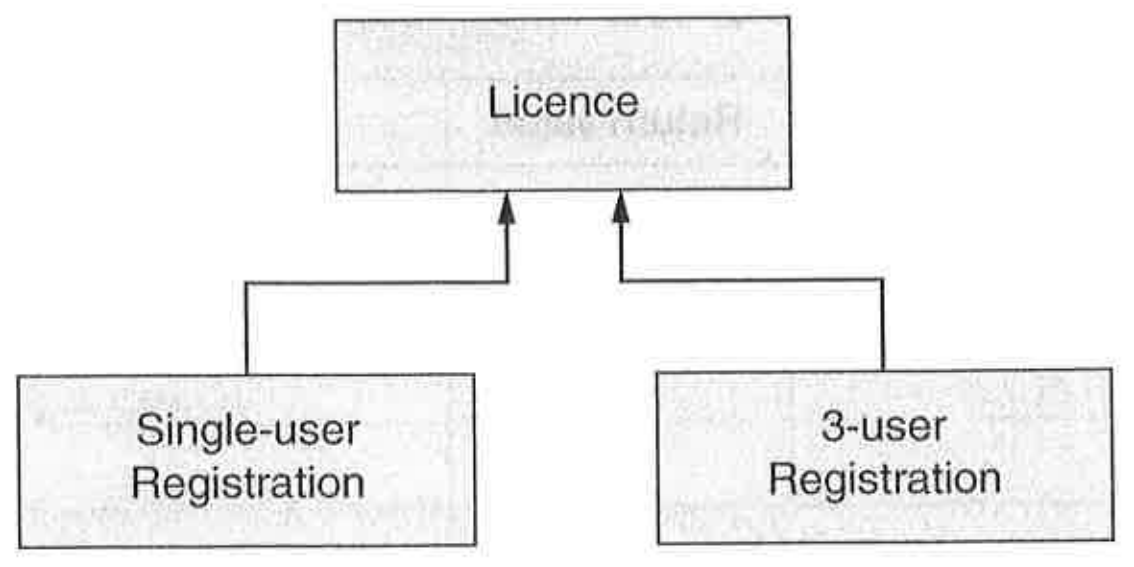
\includegraphics[width=0.5\paperwidth]{C:/Users/Admin/Desktop/Github/question_bank/LyX/static/img/9597-ALVL-2015-P1-Q3}
\par\end{center}

\subsubsection*{Task 3.5}

Write program code \textbf{only} for the three classes shown. 

Do not attempt to develop the application further.

\subsubsection*{Evidence 12}
\begin{itemize}
\item Program code for the three classes.\hfill{}{[}9{]}
\end{itemize}

 \newpage 

\item \textbf{{[}ALVL/9597/2015/P1/Q4{]} }

Users of a local area network each have a network account ID. The
IDs have the format 2015\_NNNN. where N is a digit. 

\subsubsection*{Task 4.1}

Complete the test case table with the addition of \textbf{three} more
invalid User IDs. The reasons for their invalidity should be different. 

The return value is a code as follows: 
\begin{itemize}
\item 0 - valid User lD 
\item 1 - the User ID was not 9 characters 
\item you will use other integer numbers for other invalid cases. 
\begin{center}
\begin{tabular}{|>{\centering}p{0.1\columnwidth}|>{\centering}p{0.1\columnwidth}|c|c|}
\hline 
Test Number & User ID & Return value & Explanation of the test case\tabularnewline
\hline 
1 & \texttt{2015\_0987} & \texttt{0} & Valid User ID\tabularnewline
\hline 
2 &  &  & \tabularnewline
\hline 
3 &  &  & \tabularnewline
\hline 
4 &  &  & \tabularnewline
\hline 
\end{tabular}
\par\end{center}

\end{itemize}
\hfill{}{[}10{]}

\subsubsection*{Evidence 13}
\begin{itemize}
\item The completed test case table. \hfill{}{[}6{]}
\end{itemize}

\subsubsection*{Task 4.2}

Write program code for a function to validate a User ID. The function
header has the format: 
\begin{center}
\texttt{FUNCTION ValidateUserID (ThisUserID : STRING) RETURNS INTEGER }
\par\end{center}

Write a program to:
\begin{itemize}
\item Input an ID entered by the user 
\item Validate the input using the function\texttt{ ValidateUserID }
\item Output a message describing the validity of the input. 
\end{itemize}
\hfill{}{[}10{]}

\subsubsection*{Evidence 14}
\begin{itemize}
\item Program code for the function \texttt{ValidateUserID} \hfill{}{[}4{]}
\item \textbf{Three} screenshots showing the testing of Test Numbers 2,
3, and 4. \hfill{}{[}3{]}
\end{itemize}
You are to design an object-oriented program which simulates a print
queue for a printer on a local area network (LAN).The print queue
consists at any time of none, one, or more print jobs. 

Each user can send a print job from any of the terminals on the LAN.
Each terminal on the network is identified by an integer number in
the range 1 to 172. 

The program you are to design will record for each printjob: 
\begin{itemize}
\item the user lD
\item the terminal number from which the print request was sent
\item the file size (integer in Kbytes).
\end{itemize}
In practice, there are several print queues each associated with a
different printer. Each printer is identified by a short name, such
as \texttt{Room16}. 

Task 4.3

Design and write program code to define one or more classes and other
appropriate data structures for this application. 

\subsubsection*{Evidence 15}

Program code for the class(es). \hfill{}{[}6{]} 

A print queue behaves as a queue data structure. 

Assume, for testing purposes: 
\begin{itemize}
\item there is a single printer on the LAN 
\item the maximum print queue size for the printer is five print jobs. 
\end{itemize}
The main program will simulate: 
\begin{itemize}
\item the sending of print jobs to the printer by different users 
\begin{itemize}
\item that is, the addition of a print job to the print queue 
\end{itemize}
\item the output of a job from the print queue 
\begin{itemize}
\item that is, the removal of a print job from the print queue 
\end{itemize}
\end{itemize}
The program design has the following menu: 
\begin{center}
\noindent\ovalbox{\begin{minipage}[t]{1\columnwidth - 2\fboxsep - 0.8pt}%
\begin{enumerate}
\item[1]  New print job added to print queue 
\item[2] Next print job output from printer
\item[3] Current print queue displayed
\item[4] End
\end{enumerate}
%
\end{minipage}}
\par\end{center}

The program simulates the working of the print queue as follows: 
\begin{enumerate}
\item[1.] The empty print queue is initialised. 
\item[2.]  The program user selects menu options 1, 2 and 3 in any order. 
\item[3.]  The program user selects menu opt\textbf{two}ion 4.
\end{enumerate}

\subsubsection*{Task 4.4}

Write program code to: 
\begin{itemize}
\item display the main menu 
\item input the choice by the user 
\item run the appropriate code for the choice made.
\end{itemize}

\subsubsection*{Evidence 16}

The program code. \hfill{}{[}3{]}

\subsubsection*{Task 4.5}

Write program code to initialise the print queue for the \texttt{Room16}
printer. 

Write program code to display the current state of the print queue.

\subsubsection*{Evidence 17}

The program code for:
\begin{itemize}
\item initialising the print queue
\item output of the current print queue. \hfill{}{[}6{]}
\end{itemize}

\subsubsection*{Task 4.6}

Write program code to add a new print job to the print queue.

The requirement will be:
\begin{itemize}
\item program user enters data for the new print job
\item print job is added to the print queue.
\end{itemize}
Test the code by adding one new print job.

\subsubsection*{Evidence 18}
\begin{itemize}
\item Program code to add a new print job.
\item Screenshot following menu option 1 then menu option 3. \hfill{}{[}4{]}
\end{itemize}

\subsubsection*{Task 4.7}

Write program code to output the next print job from the printer.

This code will execute from menu option 2.

Test the code by:
\begin{itemize}
\item adding three print jobs
\item outputting the next print job.
\end{itemize}

\subsubsection*{Evidence 19}
\begin{itemize}
\item Program code to output next print job.
\item Screenshot following menu option 1 three times. then menu option 2,
and menu option 3. \hfill{}{[}6{]}
\end{itemize}

 \newpage 

\item \textbf{{[}ALVL/9597/2015/P2/Q1{]} }

The management of a university is keen to implement changes which
will result in higher student attainment. The management believes
this is possible if it collects more data about its students which
is then analysed.

Possible data that might be collected includes: assignment grades,
books taken out of the library, attendance at lectures, attendance
at tutorials, meetings with personal tutor, email exchanges with university
staff. and participation in sporting and cultural activities.

University staff are classified as either academic or management.
All data about students will be available to academic staff for viewing
and editing. Summary information, which does not identify any individual
student. will be viewable by some management staff. Students have
no access to the data.

A project working party is to be set up consisting of representatives
from across the university. The working party will define the scope
of the project. It will consider what data is to be collected. it
will also decide what the data is to be used for and consider any
potential further use of the data.

If this project has a successful outcome, the university will market
its expertise to other universities. 
\begin{enumerate}
\item Give \textbf{three} different representative members of the working
party. Justify each choice. \hfill{}{[}6{]}
\item The working party has been asked to produce a list of issues that
will be considered by the Ethics Committee of the university.

State \textbf{two} issues that could be on the list.\hfill{} {[}2{]}
\end{enumerate}
After consideration of the reports from the working party and the
Ethics Committee the university management decide to proceed with
the project. A project team is put together to design and implement
a new software system.

The initial work of the project team involves an investigation process. 
\begin{enumerate}
\item[(c)] Name \textbf{two }techniques that can be used by the project team
in the investigation process. For each technique, explain how it can
be used in this project.\hfill{} {[}6{]}
\item[(d)] A detailed report is produced following the investigation.Thls report
will form the starting point of the design stage. Describe \textbf{two}
sections of the report.\hfill{} {[}4{]}
\end{enumerate}
The project team draw up a list of activities that will be required
for the completion of the software project:
\begin{center}
\begin{tabular}{|c|l|c|}
\hline 
Activity & \texttt{\hspace{0.01\columnwidth}}Activity Description  & Expected Duration (in weeks)\tabularnewline
\hline 
A & Design solution to project & 10\tabularnewline
\hline 
B & Development of solution to project & 25\tabularnewline
\hline 
C & Produce documentation & 12\tabularnewline
\hline 
D & Testing & 30\tabularnewline
\hline 
E & implement system & 8\tabularnewline
\hline 
F & Acceptance trials & 2\tabularnewline
\hline 
\end{tabular}
\par\end{center}

A first attempt to produce a Program Evaluation and Review Technique
(PERT) chart from the activity table is: 
\begin{center}
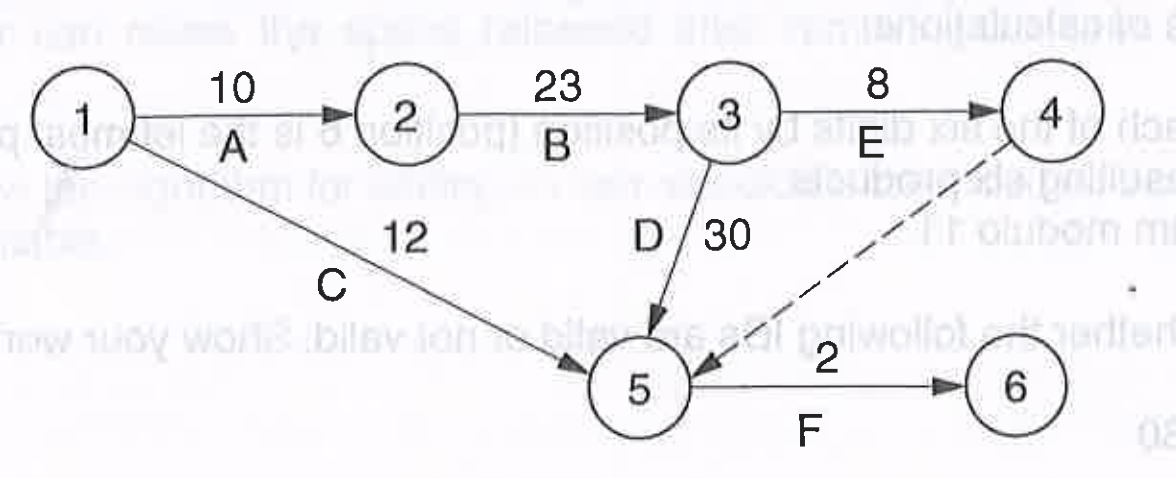
\includegraphics[width=0.5\paperwidth]{C:/Users/Admin/Desktop/Github/question_bank/LyX/static/img/9597-ALVL-2015-P2-Q1}
\par\end{center}
\begin{enumerate}
\item[(e)] {}
\begin{enumerate}
\item Describe \textbf{two} benefits that can be gained by producing a PERT
chart from the activity table. \hfill{}{[}2{]}
\item Explain the significance of the dashed line on the PERT chart. \hfill{}{[}2{]}
\item There are two errors on the PERT chart. identify these errors. Redraw
the PERT chart to show the changes needed to correct these errors.
\hfill{}{[}2{]}
\end{enumerate}
\item[(f)]  Using your PERT chart from part \textbf{(e)(iii)}: 
\begin{itemize}
\item State the minimum time in which the project could be completed.\hfill{}
{[}1{]}
\item By how many weeks can the start of the production of documentation
be delayed without delaying the whole project? \hfill{}{[}1{]}
\item Describe and give an example of concurrent activities.\hfill{} {[}2{]}
\item Describe and give an example of dependent activities. \hfill{}{[}2{]}
\end{itemize}
\end{enumerate}
Output from the system is made available to permitted staff via the
university intranet. However, the university intranet can be accessed
by all students and staff. both locally and remotely, via the lnternet.
The system needs security measures to prevent all types of unauthorised
access. 
\begin{enumerate}
\item[(g)]  Describe\textbf{ two} suitable physical security measures that could
be adopted. \hfill{}{[}4{]}
\item[(h)]  Describe \textbf{two} suitable software security measures that could
be adopted. \hfill{}{[}4{]}
\end{enumerate}
Following the success of the project, management decides that the
software system will be marketed to other universities. 
\begin{enumerate}
\item[(i)]  Explain how the university's investment in the software can be legally
protected. \hfill{}{[}2{]}
\end{enumerate}

 \newpage 

\item \textbf{{[}ALVL/9597/2015/P2/Q2{]} }

A stock control system requires that each stock item has a unique
ID consisting of six digits. The sixth digit is a check digit. This
check digit ensures that a value of 0 is the final result of the following
series of calculations:
\begin{itemize}
\item multiply each of the six digits by its position (position 6 is the
leftmost position)
\item sum the resulting six products
\item find the sum modulo 11.
\end{itemize}
\begin{enumerate}
\item Deduce whether the following IDs are valid or not valid. Show your
working. 
\begin{enumerate}
\item 810230 \hfill{}{[}2{]}
\item 371025 \hfill{}{[}2{]}
\end{enumerate}
\item The ID 483095 is a valid lD. Describe \textbf{one} typical data entry
error for this ID. Show how this error would be detected.\hfill{}
{[}3{]}
\item Describe a method of verification that can be used when an ID is entered
from a data entry form.\hfill{} {[}3{]}
\end{enumerate}

 \newpage 

\item \textbf{{[}ALVL/9597/2015/P2/Q3{]} }

A simple queue data structure is implemented using a one-dimensional
array and two pointers, Head and Tail, as shown:
\begin{center}
\begin{tabular}{r|l|l}
\multicolumn{1}{r}{} & \multicolumn{1}{l}{\texttt{Queue}} & \tabularnewline
\cline{2-2} 
\texttt{1} & \texttt{Mac} & \tabularnewline
\cline{2-2} 
\texttt{2} & \texttt{Ben} & $\impliedby$ \texttt{Head}\tabularnewline
\cline{2-2} 
\texttt{3} & \texttt{Dog} & \tabularnewline
\cline{2-2} 
\texttt{4} & \texttt{Can} & \tabularnewline
\cline{2-2} 
\texttt{5} & \texttt{Yog} & \tabularnewline
\cline{2-2} 
\texttt{6} & \texttt{Hur} & \tabularnewline
\cline{2-2} 
\texttt{7} &  & $\impliedby$ \texttt{Tail}\tabularnewline
\cline{2-2} 
\texttt{8} &  & \tabularnewline
\cline{2-2} 
\texttt{9} &  & \tabularnewline
\cline{2-2} 
\texttt{10} &  & \tabularnewline
\cline{2-2} 
\end{tabular}
\par\end{center}
\begin{enumerate}
\item Show the state of the above queue after: 
\begin{itemize}
\item two items, Dap and Eck, are added (in that order) 
\item one item is removed. \hfill{}{[}3{]}
\end{itemize}
When ten items have been added, this simple queue cannot accept any
further items. 
\item A first attempt at an algorithm for adding an item to this queue is:

\noindent\begin{minipage}[t]{1\columnwidth}%
\texttt{01 IF ..............................}

\texttt{02 \qquad{}THEN }

\texttt{03 \qquad{}\qquad{}OUTPUT \textquotedbl No more room to
add items\textquotedblright{} }

\texttt{04 \qquad{}ELSE }

\texttt{05 \qquad{}\qquad{}INPUT \textquotedbl New item to be added\textquotedbl ,
NewItem }

\texttt{06 \qquad{}\qquad{}Queue{[}..............................{]}
<- NewItem }

\texttt{O7 \qquad{}\qquad{}.............................. }

\texttt{O8 ENDIF }%
\end{minipage}

Write the pseudocode to show the completed lines 01, 06, and 07. \hfill{}{[}3{]}
\item Give the initial value for \texttt{Tail} when the queue is created
and justify your answer. \hfill{}{[}2{]}
\end{enumerate}
The programmer can reuse the space released after removing an item.
This maximises the available space.
\begin{enumerate}
\item[(d)]  Describe how the algorithm for adding an item should be amended
so that the released space is made available. \hfill{}{[}2{]}
\end{enumerate}

 \newpage 

\item \textbf{{[}ALVL/9597/2015/P2/Q4{]} }

An algorithm for converting a number n from denary to octal uses the
three built-in functions: 
\begin{center}
\begin{tabular}{|l|>{\raggedright}p{0.15\columnwidth}|>{\raggedright}p{0.25\columnwidth}|}
\hline 
\texttt{\hspace{0.01\columnwidth}}Function & \texttt{\hspace{0.01\columnwidth}}Description & \texttt{\hspace{0.01\columnwidth}}Example\tabularnewline
\hline 
\texttt{INTMOD(Number,Divisor)} & returns the remainder when the first parameter is divided by the second
parameter & \texttt{INTMOD(7,3) }returns 1\tabularnewline
\hline 
\texttt{INTDIV(Number,Divisor)} & returns the integer part when thefirst parameteris divided by the
second parameter. & \texttt{INTDIV(7,3) }returns 2\tabularnewline
\hline 
\texttt{SUBSTR(ThisString,Start,Length)} & forms a substring from ThisString, starting at Start (with first index
in string zero) and taking Length characters & \texttt{SUBSTR(``abcd'',1,2)} returns \texttt{``bc''}\tabularnewline
\hline 
\end{tabular}
\par\end{center}

Study the following pseudocode: 

\noindent %
\noindent\begin{minipage}[t]{1\columnwidth}%
\texttt{01 FUNCTION DenaryToOctal (n : INTEGER) RETURNS STRING }

\texttt{02 \qquad{}OctalDigits <- \textquotedbl 01234567\textquotedbl{} }

\texttt{03 \qquad{}IF n < 8 }

\texttt{04 \qquad{}\qquad{}THEN }

\texttt{05 \qquad{}\qquad{}\qquad{}TempString <- SUBSTR(OctalDigits,
n, 1) }

\texttt{06 \qquad{}\qquad{}ELSE }

\texttt{07 \qquad{}\qquad{}\qquad{}// '+' is the concatenation
operator }

\texttt{08 \qquad{}\qquad{}\qquad{}TempString <- DenaryToOctal(INTDIV(n,8))
+ SUBSTR(OctalDigits, INTMOD(n,8),1)) }

\texttt{09 \qquad{}ENDIF }

\texttt{10 \qquad{}RETURN TempString }

\texttt{11 ENDFUNCTION }%
\end{minipage}
\begin{enumerate}
\item Identify where and why this is a recursive function. \hfill{}{[}2{]}
\end{enumerate}
The diagram shows the execution of the call \texttt{DenaryToOctal(39)}. 
\begin{center}
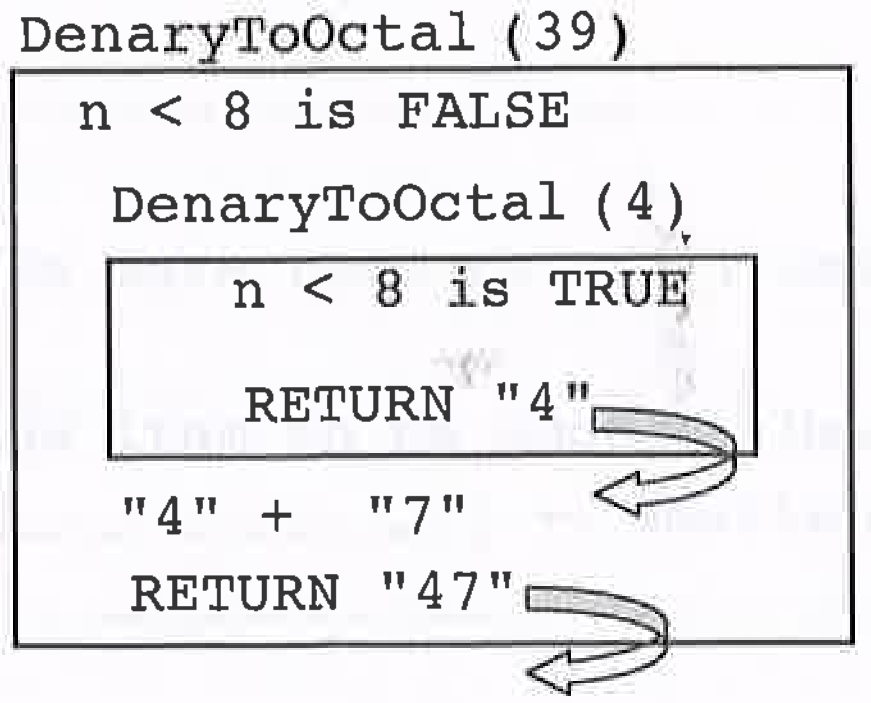
\includegraphics[width=0.5\paperwidth]{C:/Users/Admin/Desktop/Github/question_bank/LyX/static/img/9597-ALVL-2015-P2-Q4}
\par\end{center}
\begin{enumerate}
\item[(b)] Draw a similar diagram to show the execution of the call \texttt{DenaryToOctal(67)}.\hfill{}
{[}3{]}
\item[(c)] Changes are to be made to the function \texttt{DenaryToOctal()} so
that it converts denary numbers to hexadecimal.

Describe the changes: 
\begin{itemize}
\item that are essential to make the revised function work. 
\item that are non-essential but would help with the clarity of the pseudocode.\hfill{}
{[}5{]}
\end{itemize}
\end{enumerate}

 \newpage 

\item \textbf{{[}ALVL/9597/2015/P2/Q5{]} }

A program is to be written to test an insertion sort algorithm. A
top-down approach was used in the design of the program. The program,
\texttt{InsertionSortTester}, has a number of parts: 
\begin{itemize}
\item input integer values into the array 
\item output the initial values in the array 
\item output the sorted values in the array
\item perform the insertion sort 
\item validate the values 
\end{itemize}
\begin{enumerate}
\item Draw a diagram, which exhibits top-down design, for the \texttt{InsertionSortTester}
program. \hfill{}{[}3{]}

A list of data items is stored in the array \texttt{Values}. The pseudocode
for the insertion sort algorithm is: 

\noindent\begin{minipage}[t]{1\columnwidth}%
\texttt{01 FOR i <- 2 TO Arraysize }

\texttt{02 \qquad{}Temp <- Values{[}i{]} }

\texttt{03 \qquad{}j <- i\textemdash l }

\texttt{04 \qquad{}WHILE (j > 0) AND (Values {[}j{]} > Temp) }

\texttt{05 \qquad{}\qquad{}Values{[}j+1{]} <\textemdash{} Values
{[}j{]} }

\texttt{06 \qquad{}\qquad{}j <- j\textemdash l }

\texttt{07 \qquad{}\qquad{}ENDWHILE }

\texttt{08 \qquad{}\qquad{}Values {[}j+1{]} <- Temp }

\texttt{09 ENDFOR }%
\end{minipage}
\item The sort algorithm is to be tested using the sequence of numbers:
6, 8, 2 and 1. Copy and complete the trace table given below. 
\begin{center}
\begin{tabular}{|c|c|c|c||c|c|c|}
\hline 
\multicolumn{4}{|c||}{\texttt{Values}} &  &  & \tabularnewline
\hline 
\texttt{{[}1{]}} & \texttt{{[}2{]}} & \texttt{{[}3{]}} & \texttt{{[}4{]}} & \texttt{i} & \texttt{j} & \texttt{Temp}\tabularnewline
\hline 
\hline 
6 & 8 & 2 & 1 &  &  & \tabularnewline
\hline 
 &  &  &  &  &  & \tabularnewline
\hline 
 &  &  &  &  &  & \tabularnewline
\hline 
 &  &  &  &  &  & \tabularnewline
\hline 
 &  &  &  &  &  & \tabularnewline
\hline 
 &  &  &  &  &  & \tabularnewline
\hline 
 &  &  &  &  &  & \tabularnewline
\hline 
 &  &  &  &  &  & \tabularnewline
\hline 
 &  &  &  &  &  & \tabularnewline
\hline 
 &  &  &  &  &  & \tabularnewline
\end{tabular}
\par\end{center}

\hfill{}{[}6{]}
\item Explain why this particular algorithm is inefficient for an array
where the initial values are already in order.\hfill{} {[}2{]}
\item Give \textbf{two} different test cases for the program. Justify your
selection in each case.\hfill{} {[}4{]}
\end{enumerate}

 \newpage 

\item \textbf{{[}ALVL/9597/2015/P2/Q6{]} }

Students from several schools are entered for examinations in different
subjects. 

A relational database is to be used by the examination board to store
data about examination entries and results. Four tables present in
the database are STUDENT, SCHOOL, SUBJECT and STUDENT-SUBJECT.

Every time a student registers for a subject examination. a new row
is created in the STUDENT-SUBJECT table. When the result becomes available,
this is added to the appropriate row.

Each student, each school, and each subject has a unique identification
code.
\begin{enumerate}
\item {}
\begin{enumerate}
\item Draw an Entity-Relationship (E-R) diagram to show the relationship
between the STUDENT table and the SUBJECT table. \hfill{}{[}1{]}
\item State the type of relationship that exists between the STUDENT and
SUBJECT tables. \hfill{}{[}1{]}
\end{enumerate}
\item Draw an E-R diagram to show the relationship between the four tables
that provides for a fully normalised database design.\hfill{} {[}3{]}
\end{enumerate}
A table description can be expressed as: 

\texttt{TableName(Attribute1, Attribute2, Attribute3, ...)} 

The primary key is indicated by underlining one or more attributes. 

An incomplete STUDENT table is: 

\texttt{STUDENT(}\texttt{\uline{StudentID}}\texttt{, StudentName,
DateOfBirth) }
\begin{enumerate}
\item[(c)]  Give a table description for the SUBJECT table. Ensure there are
\textbf{two} attributes in addition to the primary key. \hfill{}{[}3{]}
\item[(d)]  Give a table description for the STUDENT-SUBJECT table. Ensure there
is \textbf{one} non-key attribute.\hfill{} {[}3{]}
\item[(e)] {} 
\begin{enumerate}
\item State the type of relationship that exists between the STUDENT and
the SCHOOL tables.\hfill{} {[}1{]}
\item Explain how the relationship between the STUDENT table and the SCHOOL
table is established. \hfill{}{[}3{]}
\end{enumerate}
\end{enumerate}

 \newpage 

\item \textbf{{[}DHS/PRELIM/9597/2015/P1/Q1{]} }

The coming General Election will see 28481 voters in the MacPherson
Single Member Constituency (SMC) voting for their Member of Parliament
(MP). The data file \texttt{ELECTION.txt} contains the simulated voting
results, with A, B, C and V representing votes for the political parties
National Solidarity Party, People Action Party and Workers' Party,
as well as void votes respectively. 

\subsection*{Task 1.1}

Determine the winner and the voting statistics (correct to 1 decimal
place) for this SMC. Your output should look like the following: 

Sample output: 

\noindent %
\noindent\begin{minipage}[t]{1\columnwidth}%
\texttt{Results for the Electoral Division of MacPherson }

\texttt{PAP 58.7\%}

\texttt{WP 37.5\%}

\texttt{NSP 2.6\% }

\texttt{Void 1.2\%}

\texttt{Winner is PAP }%
\end{minipage}

\subsection*{Evidence 1 }

Program code. \hfill{}{[}7{]}

\subsection*{Evidence 2}

Screenshot.\hfill{} {[}1{]}

\subsection*{Task 1.2}

In the event of a tie, the parties tied will enter into a revoting
exercise. For example, if there is a tie between PAP and WP, return
the message \textquotedbl\texttt{Revote between PAP and WP}\textquotedbl . 

Write program code to generate a text file \texttt{TIE.txt} with approximately
3\% void votes, 7\% votes for NSP and a tie between PAP and WP. Test
your program with your generated \texttt{TIE.txt}. 

\subsection*{Evidence 3 }

Program code.\hfill{} {[}6{]}

\subsection*{Evidence 4 }

Screenshot. \hfill{}{[}1{]}

 \newpage 

\item \textbf{{[}DHS/PRELIM/9597/2015/P1/Q2{]} }

You are provided with the registration dates and email addresses of
participants who registered for an event in the text file \texttt{PARTICIPANTS.txt}.
Unfortunately, some participants registered more than once. 

\subsection*{Task 2.1 }

Write program code to remove duplicate entries and generate the final
participant list in alphabetical email order. If a participant registered
more than once, take the last registered record as the final entry.
Return also a count of duplicate entries removed. 

Sample output:

\noindent %
\noindent\begin{minipage}[t]{1\columnwidth}%
\texttt{ali@yahoo.com,03-05-2015}

\texttt{dave@savetheworld.org,05-05-2015 }

\texttt{james007@bond.uk,07-05-2015}

\texttt{limahseng@gmail.com,01-05-2015 }

\texttt{mary\_ong@m1.com.sg,05-05-2015 }

\texttt{zorro@outlook.com,30-04-2015 }

\texttt{3 duplicate entries removed.}%
\end{minipage}

\subsection*{Evidence 5 }

Program code. \hfill{}{[}4{]}

\subsection*{Evidence 6 }

Screenshot.\hfill{} {[}1{]}

\subsection*{Task 2.2 }

Some email addresses may be entered wrongly. Using first principles,
write a Boolean function \texttt{Valid\_Email(email)} to determine
if an email address is valid. Design test cases to thoroughly test
the working of your function code. 

\subsection*{Evidence 7 }

Program code.\hfill{} {[}6{]}

\subsection*{Evidence 8}

Test data with purpose and corresponding screenshots. \hfill{}{[}4{]}

 \newpage 

\item \textbf{{[}DHS/PRELIM/9597/2015/P1/Q3{]} }

International Standard Book Number (ISBN) is a unique number assigned
to each edition of a book. It has two formats: ISBN-10 and ISBN-13.
The former is used before 1 Jan 2007 and the latter after that. Examples
of valid ISBNs are 020103803X and 978-1-284-05591-7. The last digit
is the check digit and is computed as follows:

\textbf{ISBN check digit (10 digits) - mod 11 algorithm} 
\begin{itemize}
\item Each digit starting from left to right is assigned a weight from 1
to 9. Each digit is multiplied by its position weight. The sum of
products modulo 11 gives a remainder between 0 and 10. If the remainder
is 10, the check digit is the roman numeral X, else the check digit
is the remainder.
\item \textbf{Example ISBN-10: 0-07-063546-3 }

$(0\times1)+(0\times2)+(7\times3)+(0\times4)+(6\times5)+(3\times6)+(5\times7)+(4\times8)+(6\times9)=190$
\item $190\mod11=3$
\item Hence 3 is the check digit. 
\end{itemize}
\textbf{ISBN check digit (13 digits) - mod 10 algorithm}
\begin{itemize}
\item Each digit starting from the left to right is multiplied by 1 or 3
alternatively. The sum of the products modulo 10 gives a remainder
between 0 to 9. If the remainder is nonzero, subtract this from 10
to get the check digit, else the check digit is 0. 
\item Example ISBN-13: 978-0-07-063546-3 

$1\times9+3\times7+1\times8+3\times0+1\times0+3\times7+1\times0+3\times6+1\times3+3\times5+1\times4+3\times6=117$
\item $117\mod10=7$
\item $10-7=3$ 
\item Hence 3 is the check digit. 
\end{itemize}

\subsection*{Task 3.1}

Write a function \texttt{ISBN\_Check\_Digit(isbn)} which generates
the check digit for a given ISBN-10 or ISBN-13 number. 

\subsection*{Evidence 9 }

Program code. \hfill{}{[}5{]}

\subsection*{Evidence 10 }

Screenshots (1 for ISBN-10 and 1 for ISBN-13)\hfill{} {[}2{]}

\subsection*{Task 3.2 }

Write a function \texttt{Valid\_ISBN(isbn)} which calls your \texttt{ISBN\_Check\_Digit(isbn)}
function in Task 3.1 to determine if a given ISBN-10 or ISBN-13 number
is valid. 

\subsection*{Evidence 11 }

Program code. \hfill{}{[}4{]}

\subsection*{Evidence 12 }

Screenshots for appropriately generated ISBN-10 and ISBN-13 numbers.\hfill{}
{[}2{]}

An ISBN-10 number can be converted to its ISBN-13 equivalent by prefixing
'978' to the ISBN-10 number and then calculating the check digit using
the ISBN-13 algorithm. 

\subsection*{Task 3.3 }

Write a function \texttt{ISBN10\_To\_ISBN13(isbn)} to convert an ISBN-10
number to its ISBN13 equivalent.

\subsection*{Evidence 13 }

Program code. \hfill{}{[}3{]}

\subsection*{Evidence 14 }

Screenshot of output for ISBN-10 number 1904467520. \hfill{}{[}1{]}

\subsection*{Task 3.4}

Write a function \texttt{ISBN13\_To\_ISBN10(isbn)} to convert an ISBN-13
number to its ISBN10 equivalent.

\subsection*{Evidence 15 }

Program code. \hfill{}{[}4{]}

\subsection*{Evidence 16 }

Screenshot of output for ISBN-13 number 9780748740468. \hfill{} {[}1{]}

A small library wishes to store its book collection details using
a random file organisation. It currently holds 200 books but wishes
to expand its collection by about 10\% every year. To resolve collisions,
it decides to use double hashing which minimises clustering. For a
start, assume that this file organisation will be maintained for 3
years. 

\subsection*{Task 3.5 }

Devise and implement a suitable double hashing strategy \texttt{Hash\_Key(isbn)}.
Annotate your strategy using program comments. 

\subsection*{Evidence 17}

Program code with comments. \hfill{}{[}5{]}

\subsection*{Task 3.6}

Write program code to generate an appropriate number of ISBNs to the
random text file \texttt{LIBRARY.txt} which will cater to the library's
collection growth over 3 years. Include \texttt{Insert\_Book(isbn)}
and \texttt{Lookup\_Book(isbn)} functions to insert a book and lookup
a book respectively. 

\subsection*{Evidence 18}

Program code. \hfill{} {[}8{]}

\subsection*{Evidence 19 }

Screenshots showing the insertion and lookup of one non-collided record
and one collided record. \hfill{}{[}4{]}

\subsection*{Evidence 20 }

Separate printout of \texttt{LIBRARY.txt} after insertion of all generated
records. \hfill{} {[}2{]}

 \newpage 

\item \textbf{{[}DHS/PRELIM/9597/2015/P1/Q4{]} }

You are tasked to maintain a binary search tree for optimal search
efficiency. Each node of the binary search tree contains a unique
identifier (productid) and a reference to a linked list which holds
individual order details for that product. For simplicity, orderid
will suffice. 

\subsection*{Task 4.1 }

Using object-oriented programming, implement the above binary search
tree with its associated class methods (\texttt{insert()}, \texttt{search()}
and \texttt{inorder()}). 

\subsection*{Evidence 21}

Program code for binary search tree with 8 products inserted, 3 of
which has at least 2 orders. \hfill{}{[}8{]}

\subsection*{Evidence 22}

Screenshot of output of inorder traversal (product and order information).
\hfill{} {[}2{]}

\subsection*{Task 4.2 }

Write a support class method most\_popular() to determine the best
selling product(s). 

\subsection*{Evidence 23 }

Program code. \hfill{} {[}4{]}

\subsection*{Evidence 24 }

Screenshot. \hfill{}{[}1{]}

\subsection*{Task 4.3 }

A product is no longer available. Write a class method delete() to
remove this node from the binary search tree, accounting for all possible
cases. 

\subsection*{Evidence 25 }

Program code. \hfill{} {[}5{]}

\subsection*{Evidence 26 }

Screenshots. \hfill{} {[}3{]}

\subsection*{Task 4.4 }

After a series of insertion and deletion, the binary search tree may
become unbalanced and this requires reorganisation to maintain optimal
search efficiency. Write functions \texttt{is\_balanced()} to test
if a binary search tree is balanced, and \texttt{reorg()} to reorganise
an unbalanced binary search tree. Include appropriate annotation.

\subsection*{Evidence 27 }

Program code. \hfill{}{[}7{]}

 \newpage 

\item \textbf{{[}DHS/PRELIM/9597/2015/P2/Q1{]} }

A young family decides to purchase a new car. The following precedence
table shows the constituent activities with their preceding activities
and durations. 
\noindent \begin{center}
\begin{tabular}{|c|c|c|c|}
\hline 
Activity & Description & Preceding Activity & Duration (days) \tabularnewline
\hline 
A & Decide feasibility of purchase & - & 3\tabularnewline
\hline 
B & Find buyer for existing car & A & 14\tabularnewline
\hline 
C & Decide on possible models & A & 1\tabularnewline
\hline 
D & Investigate decided models & C & 2\tabularnewline
\hline 
E & Discuss with knowledgeable friends & C & 1\tabularnewline
\hline 
F & Get information from dealers & C & 2\tabularnewline
\hline 
G & Put together all information & D, E, F & 1\tabularnewline
\hline 
H & Shortlist three options & G & 1\tabularnewline
\hline 
I & Test drive shortlisted options & H & 3\tabularnewline
\hline 
J & Get finance information & H & 2\tabularnewline
\hline 
K & Confirm car model & I, J & 2\tabularnewline
\hline 
L & Compare dealers and choose one & K & 2\tabularnewline
\hline 
M & Decide on colour & L & 4\tabularnewline
\hline 
N & Test drive chosen model & L & 1\tabularnewline
\hline 
O & Buy new car & B, M, N & 3\tabularnewline
\hline 
\end{tabular}
\par\end{center}
\begin{enumerate}
\item Discuss how the family can conduct a feasibility study for the purchase.\hfill{}
{[}3{]}
\item Construct a PERT chart for this project. \hfill{}{[}4{]}
\item State the critical path and the total time required for the project.
\hfill{}{[}2{]}
\item Name a floating task and state its role in the project.\hfill{} {[}2{]}
\item Explain the significance of dummy activities in this project.\hfill{}
{[}3{]}
\item Construct the corresponding Gantt chart for the project. \hfill{}{[}3{]}
\item Why should one derive the PERT chart before the Gantt chart?\hfill{}{[}2{]}
\item How does a Gantt chart help in the project?\hfill{} {[}3{]}
\item Suggest two reasons why activity M requires 4 days. What can be done
to speed this up?\hfill{} {[}3{]}
\item In activity E, the family decides to use a cross-platform mobile messaging
app which allows users to exchange messages without having to pay
for SMS. Communication with its network of knowledgeable friends requires
the use of TCP/IP sockets. What is a TCP/IP socket and how does it
help in network communication? \hfill{}{[}3{]}
\item A number of activities require the use of an Internet search engine.
Explain how an Internet search engine works and how cloud computing
is used in implementing an Internet search engine. \hfill{}{[}8{]}
\item After the car purchase, the family decides to share their experience
using either a personal blog post or a social network post to benefit
other potential car buyers. Compare the relative pros and cons of
using these approaches. \hfill{}{[}4{]}
\end{enumerate}

 \newpage 

\item \textbf{{[}DHS/PRELIM/9597/2015/P2/Q2{]} }

In a social network, each user has a public profile name and can make
zero or more posts. Each post contains a message and can be liked
by the poster and/or other users. 
\begin{enumerate}
\item Draw an E-R diagram that shows the tables and the relationships between
them. \hfill{}{[}3{]}
\item Design a normalised relational database schema. \hfill{}{[}6{]}
\item Using your answer in (b), explain the concepts of 
\begin{enumerate}
\item primary key \hfill{} {[}2{]}
\item composite key \hfill{}{[}2{]}
\item foreign key \hfill{} {[}2{]}
\end{enumerate}
\end{enumerate}

 \newpage 

\item \textbf{{[}DHS/PRELIM/9597/2015/P2/Q3{]} }

Some game tournament such as badminton, bridge, chess, Pokemon, Scabble,
and many eSports employ the Swiss system of play, in which players
are not eliminated after each round and are paired with players with
the same number of wins or as close as possible. The following shows
an example of a 16-player Scrabble tournament. Assume that all games
have a winner and there are no draws. 

First round pairing is by random draw i.e there will be 8 random pairs.
After round 1, there will be a group of 8 players with a score of
1 (win), and a group of 8 players with a score of 0 (loss). 

For the second round, players in each scoring group will be paired
against each other -- 1\textquoteright s versus 1\textquoteright s
and 0\textquoteright s versus 0\textquoteright s.

After round 2, there will be three scoring groups: 
\begin{itemize}
\item 4 players who have won both games and have 2 points 
\item 8 players who have won a game and lost a game and have 1 point
\item 4 players who have lost both games and have no points. 
\end{itemize}
Again, for the third round, players are paired with players in their
scoring group. After round 3, the typical scoring groups will be: 
\begin{itemize}
\item 2 players who have won 3 games (3 points) 
\item 6 players with 2 wins (2 points) 
\item 6 players with 1 win (1 point) 
\item 2 players with no wins (0 points) 
\end{itemize}
For the fourth (and in this case final) round, the process repeats,
and players are matched with others in their scoring group. Note that
there are only 2 players who have won all of their games so far --
they will be matched against each other for the \textquotedbl championship\textquotedbl{}
game. After the final round, we will have something that looks like
this: 
\begin{itemize}
\item 1 player with 4 points -- the winner! 
\item 4 players with 3 points -- tied for second place
\item 6 players with 2 points 
\item 4 players with 1 point 
\item 1 player with 0 points 
\end{itemize}
The Swiss system produces a clear winner in just a few rounds, no
one is eliminated and almost everyone wins at least one game, but
there are many ties to deal with. 
\begin{enumerate}
\item Propose and justify a suitable data structure to store and initialise
the player names, intermediate and final opponents, points and results
of the 16-player tournament. You may denote the players' names with
the alphabets A -- P. \hfill{} {[}3{]}
\item Devise an algorithm to update the data structure in (a) and determine
the final ranks of the players. Players who are tied will have their
names output in alphabetical order. The next rank after 2 is 3. \hfill{}{[}7{]}
\end{enumerate}

 \newpage 

\item \textbf{{[}DHS/PRELIM/9597/2015/P2/Q4{]} }

A durian specialty business sells its different breeds of durians
via two modes currently: 
\begin{itemize}
\item phone order via calling in to its sales hotline
\item web order via making an online order on its website 
\end{itemize}
For phone order, a sales agent will record the order details (breed,
quantity, customer name and phone number). Payment terms will be cash
on collection only. For web order, the customer will register for
an account using his/her email address and select the breed and quantity,
and enter his/her phone number. Payment terms will be either cash
on collection or by entering credit card details upon checkout.
\begin{enumerate}
\item Using suitable examples from this context, explain the concepts of
\begin{enumerate}
\item validation \hfill{}{[}2{]}
\item verification \hfill{}{[}2{]}
\end{enumerate}
\item Draw a UML class diagram to show the relationship between the different
types of orders.\hfill{}{[}4{]}
\item Using suitable examples, explain the concepts of 
\begin{enumerate}
\item encapsulation \hfill{}{[}2{]}
\item inheritance\hfill{} {[}2{]}
\item polymorphism \hfill{}{[}2{]}
\end{enumerate}
\item To cater to an aging population and elderly who face difficulty using
smartphones, it is proposed that an SMS application be developed to
allow elderly to order durians using SMS. Design and justify a suitable
user interface and workflow. Assume that the SMS sales number is 88387426
(88DURIAN).\hfill{} {[}3{]}
\end{enumerate}

 \newpage 

\item \textbf{{[}DHS/PRELIM/9597/2015/P2/Q5{]} }

You have taken over the following program module A in an unnamed programming
language written by an unnamed intern (who did not take A-level Computing)
to determine the number of markers and their consecutive labels to
be positioned on a newly completed highway. X is the length of the
highway in kilometres. Makers should be spaced 500 metres apart from
one another. 

\noindent %
\noindent\begin{minipage}[t]{1\columnwidth}%
\texttt{1 FUNCTION A(X : REAL) }

\texttt{2 FOR I FROM ONE TO X/500 DO }

\texttt{3 PRINT(I) }

\texttt{4 PRINT(\textquotedbl NUMBER OF MARKERS = \textquotedbl{}
+ X /500) }%
\end{minipage}
\begin{enumerate}
\item How can you improve on the programming style for the above program
module? \hfill{}{[}2{]}
\item Identify and correct the errors in the above program. Explain the
different types of errors identified.\hfill{} {[}4{]}
\item Design and justify suitable black box and white box tests for the
above program module. \hfill{}{[}4{]}
\end{enumerate}

 \newpage 

\item \textbf{{[}DHS/PRELIM/9597/2015/P2/Q6{]} }

The following figure shows a Scrabble game board.
\begin{center}
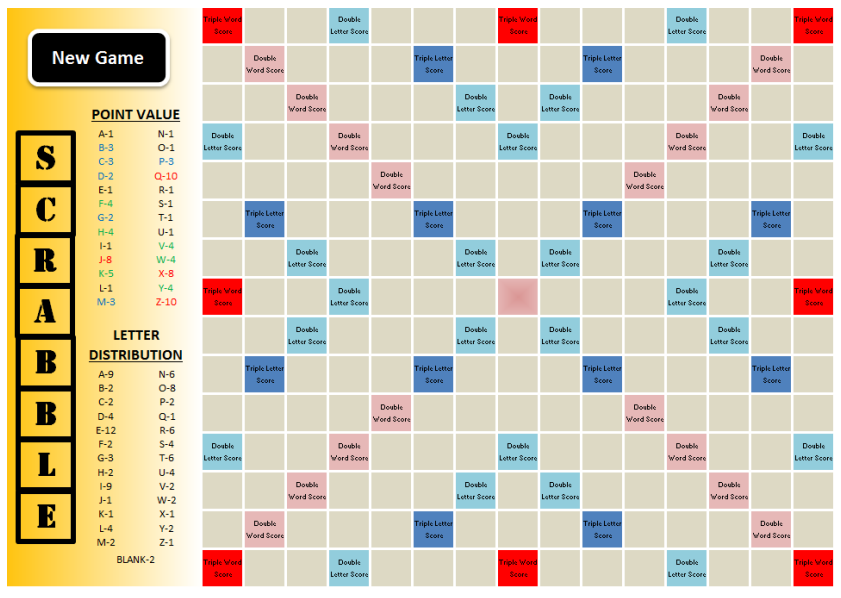
\includegraphics[width=0.65\paperwidth]{C:/Users/Admin/Desktop/Github/question_bank/LyX/static/img/9597-DHS-2015-P1-Q6-1}
\par\end{center}

Propose and justify
\begin{enumerate}
\item an efficient data structure to store the letter point values \hfill{}{[}3{]}
\item an efficient data structure to store the game board \hfill{}{[}3{]}
\item an efficient algorithm to compute the score of a word \hfill{}{[}4{]}
\end{enumerate}

 \newpage 

\item \textbf{{[}HCI/PRELIM/9597/2015/P1/Q1{]} }

A program is to process the total points of football league teams
based on number of wins, draws and losses. The program can be run
every day. 

The program reads from file \texttt{TOP\_TEAM.txt} the current highest
points and team name from running the program on previous days. 

The program specification is to: 
\begin{itemize}
\item input \textbf{up to} four team names (max. 12 characters long) each
with the total number match wins, draws and losses so far.
\item calculate the total aggregate point for each team based on 3 points
for every win, 1 point for every draw and 0 points for every loss. 
\item display on screen: 
\begin{itemize}
\item the highest point with the team name for today 
\item a message saying whether or not the highest point today beat the current
team with the highest aggregate points. 
\end{itemize}
\item update the file \texttt{TOP\_TEAM.txt} if a higher aggregate point
was computed today. 
\end{itemize}

\subsection*{Task 1.1 }

Write program code for this task. 

\subsection*{Evidence 1: }

Your program code for Task 1.1. \hfill{}{[}8{]}

\subsection*{Task 1.2 }

Draw up a set of test data which tests the functioning of your program.
Consider carefully all cases which could occur for both the data input
and the two processing requirements. 

\subsection*{Evidence 2: }

A screenshot for each test case you considered. Annotate the screenshot
explaining the purpose of each test. \hfill{}{[}7{]}

 \newpage 

\item \textbf{{[}HCI/PRELIM/9597/2015/P1/Q2{]} }

The Russian peasant algorithm is an alternative method to perform
multiplication of whole numbers by consecutive application of doubling
numbers, halving numbers and addition. 

Consider the multiplication of \texttt{57} by \texttt{86} (= \texttt{4902}): 

Write each number side by side: 
\noindent \begin{center}
\texttt{\sout{57 ~~86}}
\par\end{center}

Double the first number and halve the second number (by performing
integer division by 2 i.e. drop the remainder).

If the second number or halving result is even, cross out this entire
row. Keep doubling, halving, and crossing out until the halving result
is 1.
\noindent \begin{center}
\noindent\begin{minipage}[t]{1\columnwidth}%
\texttt{\sout{57 ~~86}}

\texttt{\sout{114 ~43}}\texttt{ }

\texttt{\sout{228 ~21}}

\texttt{\sout{456 ~10}}

\texttt{\sout{912 ~5 }}

\texttt{\sout{1824 2 }}

\texttt{\sout{3648 1}}\texttt{ }%
\end{minipage}
\par\end{center}

Add up the remaining numbers in the first column. The total is the
product of the original numbers. 
\noindent \begin{center}
\noindent\begin{minipage}[t]{1\columnwidth}%
\texttt{~~~114}

\texttt{~~~228}

\texttt{~~~912}

\texttt{\uline{+ 3648 }}

\texttt{~~4902}%
\end{minipage}
\par\end{center}


\subsection*{Task 2.1 }

Write a function to implement the Russian peasant multiplication algorithm.
Test your function with the numbers \texttt{50} and \texttt{22}. 

\subsection*{Evidence 3: }

Your program code for Task 2.1. \hfill{} {[}7{]}

\subsection*{Evidence 4: }

Screenshot showing the output from running the program. \hfill{}
{[}1{]}

The Russian peasant algorithm is actually related to binary numbers.
Doubling a decimal number is to shift its binary equivalent left,
while halving a decimal number is to shift its binary equivalent right. 

Consider the multiplication of \texttt{13} by \texttt{12} (\texttt{=
156}) 

\noindent\begin{minipage}[t]{1\columnwidth}%
\texttt{~~~~}In Binary\texttt{ ~~~~~~~~~~~~~}In Decimal\texttt{ }

\texttt{~~~}\texttt{\sout{1101 1100}}\texttt{ ~~~~~~~~~~~}\texttt{\sout{13
12}}\texttt{ }

\texttt{~ }\texttt{\sout{11010 0110}}\texttt{ ~~~~~~~~~~~}\texttt{\sout{26
6}}\texttt{ }

\texttt{~110100 0011 ~~~~~~~~~~~52 3}

\texttt{1101000 0001 ~~~~~~~~~~104 1 }

\bigskip{}

\texttt{110100 + 1101000 = 10011100 = 156 (in decimal) }%
\end{minipage}

\subsection*{Task 2.2 }

Write a function \texttt{DecToBin()} to convert a decimal number to
its binary equivalent.

\subsection*{Evidence 5: }

Your program code for Task 2.2. \hfill{}{[}3{]}

\subsection*{Task 2.3}

Implement the Russian peasant multiplication algorithm using binary
numbers. Your program should accept 2 decimal numbers as input, convert
them to binary, and then perform the necessary operations to output
a binary string as the result. You should make use of your \texttt{DecToBin()}
function in Task 2.2. 

\subsection*{Evidence 6: }

Your program code for Task 2.3. \hfill{} {[}8{]}

\subsection*{Evidence 7: }

One screenshot showing the output from running the program code. \hfill{}
{[}1{]}

 \newpage 

\item \textbf{{[}HCI/PRELIM/9597/2015/P1/Q3{]} }

A message is encrypted and passed between two parties. To decrypt
the message, a \textquotedblleft key\textquotedblright{} is applied.
Both the sending and receiving parties hold the key which enables
them to encrypt and decrypt the message. 

An approach of cryptography is the simple substitution cipher, a method
of encryption by which each letter of a message is substituted with
another letter. The receiving party deciphers the text by performing
an inverse substitution. 

The substitution system is created by first writing out a \texttt{\emph{phrase}}.
The \texttt{\emph{key}} is then derived from the \texttt{\emph{phrase}}
by removing all the repeated letters. The \texttt{\emph{cipher text}}
alphabet is then constructed starting with the letters of the key
and then followed by all the remaining letters in the alphabet. 

Using this system, the phrase \textquotedbl\texttt{apple}\textquotedbl{}
gives us the \texttt{\emph{key}} as \textquotedbl\texttt{APLE}\textquotedbl{}
and the following substitution scheme: 

\begin{tabular}{lccccccccccccccccccccccccccc}
\textbf{Plain text alphabet:} & \texttt{a} & \texttt{b} & \texttt{c} & \texttt{d} & \texttt{e} & \texttt{f} & \texttt{g} & \texttt{h} & \texttt{i} & \texttt{j} & \texttt{k} & \texttt{l} & \texttt{m} & \texttt{n} & \texttt{o} & \texttt{p} & \texttt{q} & \texttt{r} & \texttt{s} & \texttt{t} & \texttt{u} & \texttt{v} & \texttt{w} & \texttt{x} & \texttt{y} & \texttt{z} & \tabularnewline
 & \texttt{$\downarrow$} &  &  & \texttt{$\downarrow$} &  &  &  &  &  &  &  &  &  &  &  &  &  &  &  &  &  &  &  &  &  & \texttt{$\downarrow$} & is substituted by\tabularnewline
\textbf{Cipher text alphabet:} & \texttt{A} & \texttt{P} & \texttt{L} & \texttt{E} & \texttt{B} & \texttt{C} & \texttt{D} & \texttt{F} & \texttt{G} & \texttt{H} & \texttt{I} & \texttt{J} & \texttt{K} & \texttt{M} & \texttt{N} & \texttt{O} & \texttt{Q} & \texttt{R} & \texttt{S} & \texttt{T} & \texttt{U} & \texttt{V} & \texttt{W} & \texttt{X} & \texttt{Y} & \texttt{Z} & \tabularnewline
\end{tabular}

\texttt{'a'} will be substituted by \texttt{'A'}, \texttt{'b'} will
be substituted by \texttt{'P'}, \texttt{'c'} will be substituted by
\texttt{'L'}, \texttt{'d'} will be substituted by \texttt{'E'}, \texttt{'e'}
will be substituted by \texttt{'B'}, and so on. 

\subsection*{Task 3.1 }

Write program code for a function to create cipher text using the
following specification: 
\noindent \begin{center}
\texttt{FUNCTION CreateCipher (phrase: STRING): STRING }
\par\end{center}

The function \texttt{CreateCipher} has a single parameter \texttt{phrase}
and returns the cipher text alphabet as a string. 

\subsection*{Evidence 8: }

Your program code for Task 3.1. \hfill{}{[}8{]}

\subsection*{Task 3.2 }

Write program code for a procedure \texttt{CreateCipherTest} which
does the following:
\begin{itemize}
\item read the phrases from file \texttt{PHRASES.txt} 
\item create cipher text for each of the phrases 
\item display each phrase and cipher text on the screen as follows: 

\noindent\fbox{\begin{minipage}[t]{1\columnwidth - 2\fboxsep - 2\fboxrule}%
\texttt{Phrase: apple}

\texttt{Cipher text: APLEBCDFGHIJKMNOQRSTUVWXYZ }

\texttt{... ... }

\texttt{... ... }%
\end{minipage}}
\end{itemize}

\subsection*{Evidence 9: }

Your program code for Task 3.2. \hfill{}{[}3{]}

\subsection*{Evidence 10: }

Screenshot for running Task 3.2.\hfill{} {[}1{]}

\subsection*{Task 3.3}

Write program code for a function to decrypt a message using the following
specification: 
\noindent \begin{center}
\texttt{FUNCTION Decrypt(enc\_message: STRING, cipher: STRING): STRING }
\par\end{center}

The function \texttt{Decrypt} accepts parameters \texttt{enc\_message}
and \texttt{cipher}, and returns the decrypted message as a string.
Parameter \texttt{enc\_message} is the encrypted message, and parameter
\texttt{cipher} is the cipher text alphabet.

\subsection*{Evidence 11: }

Your program code for Task 3.3.\hfill{} {[}6{]}

\subsection*{Task 3.4 }

Write program code which does the following: 
\begin{itemize}
\item read the phrase and encrypted message from file \texttt{CIPHER.txt}
\item cipher text is generated from \texttt{CreateCipher} function 
\item message is decrypted from \texttt{Decrypt} function
\item display decrypted message on the screen together with the phrase and
encrypted message 

\noindent\fbox{\begin{minipage}[t]{1\columnwidth - 2\fboxsep - 2\fboxrule}%
\texttt{Phrase: ... }

\texttt{Encrypted message: ... }

\texttt{Decrypted message: ...}%
\end{minipage}} 
\end{itemize}

\subsection*{Evidence 12: }

Your program code for Task 3.4. \hfill{}{[}3{]}

\subsection*{Evidence 13:}

Screenshot for running Task 3.4.\hfill{} {[}1{]}

\subsection*{Task 3.5 }

Write program code for a function to encrypt a message using the following
specification:
\noindent \begin{center}
\texttt{FUNCTION Encrypt(message: STRING, cipher: STRING): STRING }
\par\end{center}

The function Encrypt accepts parameters \texttt{message} and \texttt{cipher},
and returns the encrypted message as a string. Parameter \texttt{message}
is the message to be encrypted while parameter \texttt{cipher} is
the cipher text. 

\subsection*{Evidence 14: }

Your program code for Task 3.5. \hfill{}{[}4{]}

\subsection*{Task 3.6 }

Write program code which does the following: 
\begin{itemize}
\item encrypt the message: \textquotedbl\texttt{do not give up!}\textquotedbl{} 
\item use the phrase: \textquotedbl\texttt{skyhigh}\textquotedbl{} 
\item generate cipher text from \texttt{CreateCipher} function
\item message is encrypted using \texttt{Encrypt} function 
\item encrypted message is displayed on screen as follows: 

\noindent\fbox{\begin{minipage}[t]{1\columnwidth - 2\fboxsep - 2\fboxrule}%
\texttt{Phrase: skyhigh}

\texttt{Encrypted Message: ... }%
\end{minipage}}
\end{itemize}

\subsection*{Evidence 15: }

Your program code for Task 3.6. \hfill{} {[}3{]}

\subsection*{Evidence 16:}

Screenshot for running Task 3.6. \hfill{}{[}1{]}

 \newpage 

\item \textbf{{[}HCI/PRELIM/9597/2015/P1/Q4{]} }

The task is to store a dataset of students\textquoteright{} names
and test scores (max size of 20 students) as a binary tree structure.
The text file \texttt{s} stores the students\textquoteright{} names
and test scores in the following format:
\noindent \begin{center}
\texttt{<student Name>|<Score> }
\par\end{center}

All test scores are integer values in the range 0 to 100 inclusive. 

The program will use a user-defined type \texttt{Node} for each node
defined as follows: 
\begin{center}
\begin{tabular}{|l|l|l|}
\hline 
\texttt{\textbf{\hspace{0.01\columnwidth}}}\textbf{Identifier} & \texttt{\textbf{\hspace{0.01\columnwidth}}}\textbf{Data Type} & \texttt{\textbf{\hspace{0.05\columnwidth}}}\textbf{Description}\tabularnewline
\hline 
\texttt{LeftP} & \texttt{INTEGER} & The left pointer for the node\tabularnewline
\hline 
\texttt{Name} & \texttt{STRING} & The name of the student\tabularnewline
\hline 
\texttt{Score} & \texttt{INTEGER} & The score of the studen\tabularnewline
\hline 
\texttt{RightP} & \texttt{INTEGER} & The right node pointer for the node\tabularnewline
\hline 
\end{tabular}
\par\end{center}

A linked list is maintained of all the unused nodes which do not form
part of the tree. The first available node which is used for a new
student is indicated by \texttt{NextFreePosition}. Nodes in the unused
list are linked using their left pointers. 

The binary tree and linked list are implemented using variables as
follows:
\begin{center}
\begin{tabular}{|l|l|l|}
\hline 
\texttt{\textbf{\hspace{0.01\columnwidth}}}\textbf{Identifier} & \texttt{\textbf{\hspace{0.01\columnwidth}}}\textbf{Data Type} & \texttt{\textbf{\hspace{0.05\columnwidth}}}\textbf{Description}\tabularnewline
\hline 
\texttt{ThisTree} & \texttt{ARRAY{[}20{]}: Node} & The tree data\tabularnewline
\hline 
\texttt{Root} & \texttt{INTEGER} & Index for the root position of the \texttt{ThisTree} array\tabularnewline
\hline 
\texttt{NextFreePosition} & \texttt{INTEGER} & Index for the next unused node\tabularnewline
\hline 
\end{tabular}
\par\end{center}

\begin{center}
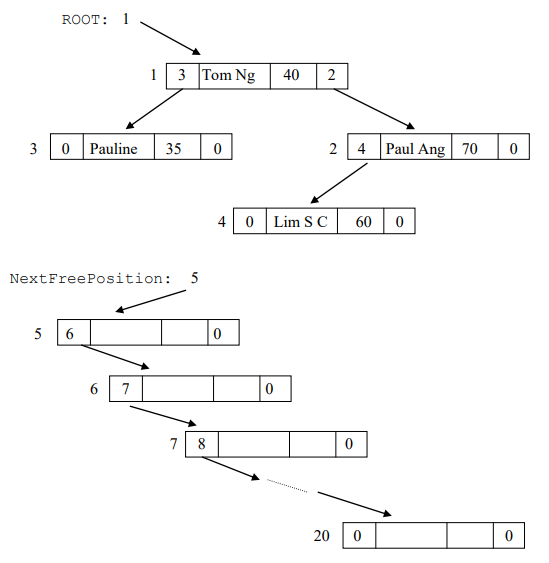
\includegraphics[width=0.65\paperwidth]{C:/Users/Admin/Desktop/Github/question_bank/LyX/static/img/9597-HCI-2015-P1-Q4-1}
\par\end{center}

The diagram shows the binary tree with the students\textquoteright{}
scores 40, 70, 35 and 60 (added in that order) and linked list of
unused nodes after the four students\textquoteright{} scores have
been added. 

\subsection*{Task 4.1 }

Write the program code to declare all the required variables and create
the initial linked list which contains all 20 nodes. Add statement(s)
to initialize the empty tree. 

\subsection*{Evidence 17: }

Your program code for Task 4.1. {[}8{]} 

The following (incomplete) pseudocode inserts a student\textquoteright s
name and his/her score into the binary tree structure. 

The \texttt{LastMove} variable holds the direction of the previous
traversal move as follows: 

X -{}- no move yet made 

L -{}- move was to the left

R -{}- move was to the right 

\noindent %
\noindent\begin{minipage}[t]{1\columnwidth}%
\texttt{PROCEDURE AddNodeToBinaryTree(NewName, NewScore) \bigskip{}
}

\texttt{IF Root = 0 }

\texttt{\qquad{}THEN }

\texttt{\qquad{}\qquad{}Root <- NextFreePosition }

\texttt{\qquad{}ELSE }

\texttt{\qquad{}\qquad{}//traverse the tree to find the position
for the new value }

\texttt{\qquad{}\qquad{}CurrentPosition <- Root }

\texttt{\qquad{}\qquad{}LastMove <- \textquoteleft X\textquoteright{} }

\texttt{\qquad{}\qquad{}REPEAT}

\texttt{\qquad{}\qquad{}\qquad{}PreviousPosition <- CurrentPosition }

\texttt{\qquad{}\qquad{}\qquad{}IF NewScore < ThisTree{[}CurrentPosition{]}.Score }

\texttt{\qquad{}\qquad{}\qquad{}\qquad{}THEN }

\texttt{\qquad{}\qquad{}\qquad{}\qquad{}\qquad{}//move left }

\texttt{\qquad{}\qquad{}\qquad{}\qquad{}\qquad{}LastMove <- \textquoteleft L\textquoteright{} }

\texttt{\qquad{}\qquad{}\qquad{}\qquad{}\qquad{}CurrentPosition
\textleftarrow{} ThisTree{[}CurrentPosition{]}.LeftP }

\texttt{\qquad{}\qquad{}\qquad{}\qquad{}ELSE}

\texttt{\qquad{}\qquad{}\qquad{}\qquad{}\qquad{}// move right }

\texttt{\qquad{}\qquad{}\qquad{}\qquad{}\qquad{}LastMove <- \textquoteleft R\textquoteright{} }

\texttt{\qquad{}\qquad{}\qquad{}\qquad{}\qquad{}CurrentPosition
\textleftarrow{} ThisTree{[}CurrentPosition{]}.RightP }

\texttt{\qquad{}\qquad{}\qquad{}ENDIF }

\texttt{\qquad{}UNTIL CurrentPosition = 0}

\texttt{ENDIF \bigskip{}
}

\texttt{IF LastMove = \textquoteleft R\textquoteright{} }

\texttt{\qquad{}THEN }

\texttt{\qquad{}\qquad{}ThisTree{[}PreviousPosition{]}.RightP <-
NextFreePosition }

\texttt{\qquad{}ELSE }

\texttt{\qquad{}\qquad{}ThisTree{[}PreviousPosition{]}.LeftP <-
NextFreePosition}

\texttt{ENDIF }

\texttt{NextFreePosition \textleftarrow{} ThisTree{[}NextFreePosition{]}.LeftP\bigskip{}
}

\texttt{ENDPROCEDURE }%
\end{minipage}

Note: The above text is available in the text file \texttt{PSEUDOCODE\_TASK\_4\_2.txt} 

\subsection*{Task 4.2 }

Write non-recursive code to implement the \texttt{AddNodeToBinaryTree}
procedure that will add a new node with student\textquoteright s name
and score into the binary tree structure. 

You may use the text file \texttt{PSEUDOCODE\_TASK\_4\_2.txt} as a
basis for the writing of your code. 

The given pseudocode is incomplete as: 
\begin{itemize}
\item it does not initially test that there is free node available for a
new student 
\item it does not assign \texttt{NewName} and \texttt{NewScore} to the data
fields of the \texttt{ThisTree} array Add these requirements to your
program solution.
\end{itemize}

\subsection*{Evidence 18: }

Your program code for Task 4.2. \hfill{} {[}6{]}

\subsection*{Task 4.3 }

Write a procedure \texttt{OutputData} which displays the value of
\texttt{Root}, the value of \texttt{NextFreePosition} and the contents
of \texttt{ThisTree} in index order.

\subsection*{Evidence 19: }

Your program code for Task 4.3. \hfill{}{[}5{]}

\subsection*{Task 4.4 }

Write a main program to: construct a binary search tree using the
data provided in the text file \texttt{SCORES.txt} by calling procedure
\texttt{AddNodeToBinaryTree} . Your program will then call procedure
\texttt{OutputData}. 

\subsection*{Evidence 20: }

Your program code for Task 4.4. \hfill{}{[}3{]}

\subsection*{Evidence 21:}

Screenshot showing the output from running the program in Task 4.4
\hfill{}{[}5{]}

\subsection*{Task 4.5 }

Write a recursive procedure \texttt{RankList} to output the students\textquoteright{}
names and scores in descending scores order. Include a call to the
procedure from your main program. Evidence 22: Your program code for
Task 4.5. {[}6{]} 

\subsection*{Evidence 23: }

Provide a screenshot showing students\textquoteright{} names and scores
in descending scores order. \hfill{} {[}2{]}

 \newpage 

\item \textbf{{[}HCI/PRELIM/9597/2015/P2/Q1{]} }
\begin{enumerate}
\item What do you understand by the usability of a user interface?\hfill{}
{[}3{]}
\item Handheld mobile devices have become increasing prevalent. Shneiderman\textquoteright s
\textquotedblleft Golden Rules of Interface Design\textquotedblright{}
have existed for some time now. Making use of the \textquotedblleft Golden
Rules\textquotedblright{} as a starting point, grounded in previous
research studies proposes a set of guidelines for mobile device interface
design. Clear explanation needed to articulate your guidelines. Use
examples if necessary to illustrate your point.\hfill{} {[}9{]}
\end{enumerate}

 \newpage 

\item \textbf{{[}HCI/PRELIM/9597/2015/P2/Q2{]} }
\begin{enumerate}
\item What are the characteristics of client-server network architecture?
\hfill{}{[}2{]} 
\item Give 2 examples of servers and explain how they function in a network.\hfill{}{[}4{]} 
\item Describe how parity bits are used to check the accuracy of a block
of bits. Give an example to support your answers. \hfill{}{[}4{]} 
\item Explain the following cloud computing concepts: 
\begin{enumerate}
\item Software as a service \hfill{}{[}1{]}
\item Platform as a service \hfill{}{[}1{]}
\item Infrastructure as a service \hfill{}{[}1{]}
\end{enumerate}
\end{enumerate}

 \newpage 

\item \textbf{{[}HCI/PRELIM/9597/2015/P2/Q3{]} }

Your company is starting the development of relational database for
a patient billing system to be marketed to private medical practices
in Singapore. The system is to be called PATMAN (short for PATient
billing MANager), and is to run as a remote client-server system and
a local area network. 

An initial analysis phase of the project has resulted in the following
description of the relevant data for PATMAN. 
\begin{itemize}
\item A practice has a number of patients and doctors. 
\item Doctors are identified by name.
\item Each patient has a number used to identify the patient called the
OHIP number, a name and an age.
\item Each patient is either a male or female and has a next of kin identified
by name.
\item Each medical procedure paid by the government of Singapore is identified
by a procedure code and has a description and a charging category.
\item Each charging category has a dollar value. 
\item Each patient has a number of billing records, with each billing record
recording the medical procedure, the date on which the procedure was
performed, the examining doctor and some additional comments on the
part of the examining doctor.
\item Billing records are either outstanding or paid in full.
\end{itemize}
\begin{enumerate}
\item Draw an ER diagram that represents the PATMAN data. \hfill{}{[}6{]}
\item Using shorthand notation, what are tables in this relational database?\hfill{}
{[}12{]}
\item Explain why relational database is better than a flat file design?\hfill{}
{[}2{]}
\end{enumerate}

 \newpage 

\item \textbf{{[}HCI/PRELIM/9597/2015/P2/Q4{]} }

The University bookstore sells books online and charges for delivery.
Its delivery charges for orders less than \$200 are as follows: 
\begin{itemize}
\item If the number of items is 3 or less, delivery by next day will be
charged at \$30, while standard delivery will be charged at \$2 per
item. 
\item If the number of items is 4 or more, delivery by next day will be
charged at \$5 per item, while standard delivery is free. 
\end{itemize}
For orders more than \$200, standard delivery is free for any number
of items, while delivery by next day will be charged at \$5 per item. 
\begin{enumerate}
\item Draw a decision table showing all the possible conditions and actions. 
\item Simplify your decision table by removing the redundancies. \hfill{}{[}5{]}
\end{enumerate}

 \newpage 

\item \textbf{{[}HCI/PRELIM/9597/2015/P2/Q5{]} }

HC university has various campuses around the city and Wilson Parking
is responsible for all the university car parks.

At each car park:

A car arriving triggers a sensor (S1) and a fixed fee (F) is paid
into a machine. This allows a barrier (B1) to be lifted and the car
to enter the car park. When a car leaves the car park it passes over
another sensor (S2) and another barrier (B2) is lifted. 

Each car park has a maximum number of spaces for cars (M) and when
this maximum is reached a \textquotedblleft FULL\textquotedblright{}
sign is illuminated at the entrance and the barrier (B1) will not
rise. The car park is closed at least once a day for cleaning purposes. 
\begin{enumerate}
\item Write an algorithm which will control the barriers and which will
keep a total (T) of the fees paid. \hfill{}{[}8{]}

There are 100 car parks, each of which is identified by a number between
1 and 100. 

At the end of each month, the total fees paid for that month (T) is
collected from each of the car parks as an integer value. 

All data are stored in an array Parks(). 
\begin{itemize}
\item For car park x, Parks(x, 1) to Parks(x, 12) contains the totals for
the twelve months of the year.
\item Parks(x, 13) contain the annual total fees collected for each car
park.
\end{itemize}
\item Using Parks(x,y) to identify individual values in the array, write
an algorithm which can be used to produce the annual totals once the
twelve monthly totals have been input to the array, and the grand
annual total for all the 100 carparks. \hfill{}{[}5{]}
\item When implementing the algorithm into program code, they should be
written to display clarity. Describe \textbf{three} features of the
final program code for this implementation that would achieve this
goal. \hfill{}{[}3{]}
\end{enumerate}

 \newpage 

\item \textbf{{[}HCI/PRELIM/9597/2015/P2/Q6{]} }

A systems analyst is developing a new computerized admission system
for HC University. 

The project manager identifies the following activities with their
durations and precedence relations: 
\noindent \begin{center}
\begin{tabular}{|c|c|c|}
\hline 
Task & Predecessors & Time(Weeks)\tabularnewline
\hline 
A & - & 3\tabularnewline
\hline 
B & - & 5\tabularnewline
\hline 
C & - & 7\tabularnewline
\hline 
D & A & 8\tabularnewline
\hline 
E & B & 5\tabularnewline
\hline 
F & C & 5\tabularnewline
\hline 
G & E & 4\tabularnewline
\hline 
H & F & 5\tabularnewline
\hline 
I & D & 6\tabularnewline
\hline 
J & G, H & 4\tabularnewline
\hline 
\end{tabular}
\par\end{center}
\begin{enumerate}
\item {}
\begin{enumerate}
\item Draw a Program Evaluation and Review Technique (PERT) chart, show
clearly the early start and late start time of each task, showing
dummy tasks, where necessary. \hfill{}{[}4{]}
\item Explain dependent stages and concurrent stages, giving examples from
your chart. \hfill{}{[}2{]}
\item State the critical path and the minimum time in which the project
can be completed. \hfill{}{[}2{]}
\end{enumerate}
\item Produce a Gantt chart based on the above information. \hfill{}{[}3{]}
\item Give \textbf{one} reason why a Gantt chart may be preferred over a
PERT chart. \hfill{}{[}1{]}
\end{enumerate}
In the current system,
\begin{itemize}
\item Each new student sends a completed form that has their name, date
of birth and the courses that they wish to enroll on. 
\item The date of birth is checked to see whether the student is of the
correct age range for admission to the college. 
\item If the student is too young or too old, a standard rejection letter
is produced. 
\item If the student is of the correct age then each of the courses that
the student has identified are checked on the course file to see whether
they are full or not. 
\item If there is room on a course then the student name is added to the
appropriate course record on the course file. 
\item A standard letter is produced with details of which course(s) the
student has been enrolled on. 
\end{itemize}
\begin{enumerate}
\item[(d)]  
\begin{enumerate}
\item Draw a data flow diagram (DFD) for the current system. \hfill{}{[}6{]}
\item Using examples from your DFD, explain how the diagram helps to inform
a database solution for the new computerized system. \hfill{}{[}4{]}
\item Give \textbf{two} parts of the database design that is not possible
from the DFD. \hfill{}{[}2{]}
\end{enumerate}
\end{enumerate}

 \newpage 

\item \textbf{{[}HCI/PRELIM/9597/2015/P2/Q7{]} }

Hash table has an index range of 1 to 400. The following pseudocode
describes an algorithm for searching the table using a hashing method.
It is assumed that the key is present in the table. 

\noindent\begin{minipage}[t]{1\columnwidth}%
\texttt{1. index = hash(key)}

\texttt{2. while table(index, 1) <> key }

\texttt{3. \qquad{}index = index + 1}

\texttt{4. endwhile }

\texttt{5. value = table(index, 2) }%
\end{minipage}
\begin{enumerate}
\item Explain the purpose of: 
\begin{enumerate}
\item line 1 
\item line 2 
\item line 3 
\item line 5 
\end{enumerate}
in this algorithm. \hfill{} {[}8{]}
\item The algorithm fails to handle the upper limit on the range of the
index. What modification to the algorithm is required to overcome
this problem? \hfill{} {[}2{]}
\end{enumerate}

 \newpage 

\item \textbf{{[}PJC/PRELIM/9597/2015/P1/Q1{]} }

\texttt{Rainfall\_mth.csv} is a file which contains monthly total
rainfall (in millimetres), for years 1984 to 2014. The format of the
record is \textquotedblleft \textbf{\emph{{[}Year{]} M {[}Month{]}
, {[}rainfall in millimetres{]}}}\textquotedblright . Three sample
records are: 
\begin{itemize}
\item \textquotedblleft \texttt{1984M01, 251.2}\textquotedblright , which
means total rainfall for January 1984 is 251.2; 
\item \textquotedblleft \texttt{1999M07, 225.4}\textquotedblright , which
means total rainfall for July 1999 is 225.4; 
\item \textquotedblleft \texttt{2014M11, 250.8}\textquotedblright , which
means total rainfall for November 2014 is 250.8.
\end{itemize}
The total annual rainfall for a particular year can be calculated
by adding the monthly total rainfall for the twelve months. 

\subsection*{Task 1.1 }

Write program code to find total annual rainfall from 1984 to 2014
and display in a table with a heading and borders as follows: 
\noindent \begin{center}
\begin{tabular}{|c|c|}
\hline 
Year & Total Annual Rainfall (millimetres in 1 d.p.)\tabularnewline
\hline 
1984 & 2686.7\tabularnewline
\hline 
1985 & 1483.9\tabularnewline
\hline 
1986 & 2536.1\tabularnewline
\hline 
... & ... ...\tabularnewline
\hline 
... & ... ...\tabularnewline
\hline 
... & ... ...\tabularnewline
\hline 
2014 & 1538.1\tabularnewline
\hline 
\end{tabular}
\par\end{center}

\subsection*{Evidence 1: }

The program code. \hfill{}{[}7{]}

\subsection*{Evidence 2:}

Screenshot to display total annual rainfall. \hfill{}{[}1{]}

\texttt{Rainfall\_day.csv} is another file which contains number of
rainy days in a month, for years 2009 to 2014. The format of the record
is \textquotedblleft {[}Year{]} M {[}Month{]} , {[}number of days{]}\textquotedblright .
Three sample record are: 
\begin{itemize}
\item \texttt{\textquotedblleft 2009M03, 19\textquotedblright }, which means
there are 19 rainy days in March 2009;
\item \texttt{\textquotedblleft 2011M05, 15\textquotedblright }, which means
there are 15 rainy days in May 2011; 
\item \texttt{\textquotedblleft 2014M09, 9\textquotedblright }, which means
there are 9 rainy days in September 2014. 
\end{itemize}
The average rainfall for a rainy day for a particular year can be
calculated by dividing the total annual rainfall by the total number
of rainy days in a year. 

\subsection*{Task 1.2 }

Amend your program code using the following specifications: 
\begin{itemize}
\item Allow user to input a year from 2009 to 2014
\item Output error message if input is outside these years -- 2009 to 2014
\item Calculate the average rainfall for a rainy day for that year
\item Output the result 
\end{itemize}

\subsection*{Evidence 3:}

Your amended program code. \hfill{}{[}5{]}

\subsection*{Evidence 4: }

Screenshots that show 2 test cases from running Task 1.2. \hfill{}{[}2{]}

 \newpage 

\item \textbf{{[}PJC/PRELIM/9597/2015/P1/Q2{]} }

Quicksort is a sorting algorithm that employs a divide-and-conquer
strategy. 

Here is a high-level description of Quicksort applied to an array
A{[}0 : n -- 1{]}: 
\begin{enumerate}
\item[1.]  Select an element from A{[}0 : n -- 1{]} to be the pivot. 
\item[2.]  Rearrange the elements of A to partition A into a left subarray
and a right subarray, such that no element in the left subarray is
larger than the pivot and no element in the right subarray is smaller
than the pivot. 
\item[3.]  Recursively sort the left and the right subarrays.
\end{enumerate}

\subsection*{Task 2.1 }

Study the identifier table and incomplete quicksort algorithm. The
missing parts of the algorithm are labelled A, B and C. 
\noindent \begin{center}
\begin{tabular}{|c|c|c|}
\hline 
Variable & Data Type & Description\tabularnewline
\hline 
\hline 
ThisArray & ARRAY OF INTEGER & Array containing the dataset\tabularnewline
\hline 
First & INTEGER & First index of array\tabularnewline
\hline 
Last & INTEGER & Last index of array\tabularnewline
\hline 
Temp & INTEGER & Temporary variable\tabularnewline
\hline 
Low & INTEGER & Index of array\tabularnewline
\hline 
High & INTEGER & Index of array\tabularnewline
\hline 
Pivot & INTEGER & Reference value in array\tabularnewline
\hline 
\end{tabular}
\par\end{center}

\noindent %
\noindent\begin{minipage}[t]{1\columnwidth}%
\texttt{FUNCTION QuickSort(ThisArray, First, Last) RETURNS NULL }

\texttt{\qquad{}DECLARE Temp:INTEGER, Low:INTEGER, High:INTEGER,
Pivot:INTEGER }

\texttt{\qquad{}Low <- First }

\texttt{\qquad{}High <- Last }

\texttt{\qquad{}.........A......... //Assign reference value }

\texttt{\bigskip{}
}

\texttt{\qquad{}WHILE Low <= High }

\texttt{\qquad{}\qquad{}WHILE(ThisArray{[}Low{]} < Pivot) //Scan
left}

\texttt{\qquad{}\qquad{}\qquad{}.........B......... }

\texttt{\qquad{}\qquad{}ENDWHILE }

\texttt{\qquad{}\qquad{}WHILE(ThisArray{[}High{]} > Pivot) //Scan
right}

\texttt{\qquad{}\qquad{}\qquad{}High <- High \textendash{} 1 }

\texttt{\qquad{}\qquad{}ENDWHILE}

\texttt{\qquad{}\qquad{}IF Low <= High //Swapping }

\texttt{\qquad{}\qquad{}\qquad{}Temp <- ThisArray{[}Low{]} }

\texttt{\qquad{}\qquad{}\qquad{}ThisArray{[}Low{]} <- ThisArray{[}High{]} }

\texttt{\qquad{}\qquad{}\qquad{}ThisArray{[}High{]} <- Temp; }

\texttt{\qquad{}\qquad{}\qquad{}Low <- Low + 1 //Shift right by
1 element}

\texttt{\qquad{}\qquad{}\qquad{}High <- High - 1 //Shift left by
1 element }

\texttt{\qquad{}\qquad{}ENDIF}

\texttt{\qquad{}ENDWHILE}

\texttt{\bigskip{}
}

\texttt{\qquad{}IF First < High }

\texttt{\qquad{}\qquad{}QuickSort(ThisArray, First, High)}

\texttt{\qquad{}ENDIF}

\texttt{\qquad{}IF Low < Last}

\texttt{\qquad{}\qquad{}.........C.........}

\texttt{\qquad{}ENDIF}

\texttt{ENDFUNCTION }%
\end{minipage}

\subsection*{Evidence 5: }

What are the three missing lines of this pseudocode?\hfill{} {[}3{]}

\subsection*{Task 2.2}

Write a program to implement the quicksort. 

The program will:
\begin{itemize}
\item Call procedure \texttt{InitialiseList}. 
\item Use the function \texttt{QuickSort} to sort an array of integer \texttt{{[}435,646,344,54,23,98,789,212,847,201,733{]}}.
Copy and paste this array from the file \texttt{Number.txt} into your
program. 
\item Output the array \uline{before} and \uline{after} the quicksort
algorithm is applied.
\end{itemize}

\subsection*{Evidence 6: }

Program code for Task 2.2.\hfill{} {[}7{]}

\subsection*{Evidence 7: }

Screenshot to show running of program code in Task 2.2.\hfill{} {[}1{]}

\subsection*{Task 2.3 }

Amend the program as follows: 

The program must also output the number of function calls carried
out. 

\subsection*{Evidence 8: }

The amended program code.\hfill{} {[}3{]}

\subsection*{Task 2.4 }

By selecting different reference values (pivot) and input datasets,
and making use of the number of function calls, evaluate the efficiency
of the algorithm. 

\subsection*{Evidence 9: }

Evaluation of efficiency of quicksort algorithm with accompanying
screenshots (showing runs of function) for different reference values
and input datasets.\hfill{} {[}4{]}

 \newpage 

\item \textbf{{[}PJC/PRELIM/9597/2015/P1/Q3{]} }

A program is to be written to find all the words in a piece of text
and to print them in alphabetical order, together with the number
of times each word occurs. The data structure used to hold this information
will be a linked list, with each node holding a word, the number of
occurrence of that word, and a pointer to the node containing the
next word in alphabetical order. 

The program will use nodes implemented as instances of the class ListNode.
The class \texttt{ListNode} has the following properties: 
\noindent \begin{center}
\begin{tabular}{|l|l|l|}
\hline 
\multicolumn{3}{|c|}{\texttt{Class: ListNode}}\tabularnewline
\hline 
\multicolumn{3}{|c|}{Properties}\tabularnewline
\hline 
\texttt{\hspace{0.01\columnwidth}}Identifier & \texttt{\hspace{0.01\columnwidth}}Data Type & \texttt{\hspace{0.05\columnwidth}}Description\tabularnewline
\hline 
\texttt{Word} & \texttt{STRING} & The node\textquoteright s value for a word from the text \tabularnewline
\hline 
\texttt{Count} & \texttt{INTEGER} & The node's value for number of occurrences of the word\tabularnewline
\hline 
\texttt{Pointer} & \texttt{INTEGER} & The pointer for the node\tabularnewline
\hline 
\end{tabular}
\par\end{center}

A linked list is implemented as an instance of the class \texttt{LinkedList}.
The class \texttt{LinkedList} has the following properties and methods: 
\noindent \begin{center}
\begin{tabular}{|l|l|l|}
\hline 
\multicolumn{3}{|c|}{\texttt{Class: LinkedList}}\tabularnewline
\hline 
\multicolumn{3}{|c|}{Properties}\tabularnewline
\hline 
\texttt{\hspace{0.01\columnwidth}}Identifier & \texttt{\hspace{0.01\columnwidth}}Data Type & \texttt{\hspace{0.05\columnwidth}}Description\tabularnewline
\hline 
\texttt{Node} & \texttt{ARRAY{[}30{]} of ListNode} & The linked list data structure -- data values (Word \& Count) and
pointers. Array index starts at 0. For testing purposes, the dataset
has a maximum of 30 nodes. \tabularnewline
\hline 
\texttt{Start} & \texttt{INTEGER} & Index position of the node at the start of the linked list\tabularnewline
\hline 
\texttt{NextFree} & \texttt{INTEGER} & Index position of the next unused node\tabularnewline
\hline 
\end{tabular}
\par\end{center}

\noindent \begin{center}
\begin{tabular}{|l|l|l|}
\hline 
\multicolumn{3}{|c|}{\texttt{Class: LinkedList}}\tabularnewline
\hline 
\multicolumn{3}{|c|}{Methods}\tabularnewline
\hline 
\texttt{\hspace{0.01\columnwidth}}Identifier & \texttt{\hspace{0.01\columnwidth}}Data Type & \texttt{\hspace{0.05\columnwidth}}Description\tabularnewline
\hline 
Initialise & PROCEDURE & Sets all node data values to empty string (for Word) and 0 (for Count).
Set pointers to indicate all nodes are unused and linked. Initialise
values for Start and NextFree.\tabularnewline
\hline 
Update & PROCEDURE & Updates the linked list with a word read from the text\tabularnewline
\hline 
Display & PROCEDURE & Display the current state of array content and pointers in table form.\tabularnewline
\hline 
IsEmpty & FUNCTION RETURNS BOOLEAN & Test for empty linked list.\tabularnewline
\hline 
IsFull & FUNCTION RETURNS BOOLEAN & Test for no unused nodes.\tabularnewline
\hline 
\end{tabular}
\par\end{center}

The diagram shows the linked list with: 
\begin{itemize}
\item the text \textquotedblleft mary had a little lamb\textquotedblright{}
added 
\item the unused nodes linked together. 
\end{itemize}
\begin{center}
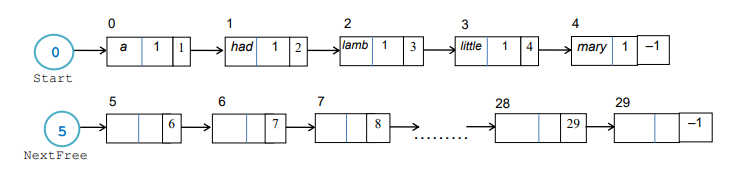
\includegraphics[width=0.65\paperwidth]{C:/Users/Admin/Desktop/Github/question_bank/LyX/static/img/9597-PJC-2015-P1-Q3-1}
\par\end{center}

\subsection*{Task 3.1}

Write the program code for the classes \texttt{ListNode} and \texttt{LinkedList},
including the \texttt{Initialise}, \texttt{Display}, \texttt{IsEmpty}
and \texttt{IsFull} method. The code should follow the specification
given. Do not write the \texttt{Update} procedure yet. 

\subsection*{Evidence 10: }

Your program code for the \texttt{ListNode} and \texttt{LinkedList}
classes. \hfill{}{[}12{]}

\subsection*{Task 3.2}

Write code to create a \texttt{LinkedList} object and run \texttt{Display}
procedure to show the content of the object. 

\subsection*{Evidence 11: }

Screenshot confirming all values after initialisation of the \texttt{LinkedList}.\hfill{}
{[}3{]}

\subsection*{Task 3.3 }

Write code to implement for the \texttt{LinkedList} class the \texttt{Update}
method that will update the linked list with a word read from the
text. 

\subsection*{Evidence 12:}

Program code for \texttt{Update} procedure. \hfill{}{[}12{]}

\subsection*{Task 3.4 }

Write code to use the Update procedure by reading in the text from
the file \texttt{Story.txt}. 

\subsection*{Evidence 13:}

Screenshot of state of array content and pointers by running \texttt{Display}
procedure. \hfill{}{[}4{]}

\subsection*{Task 3.5 }

Write a method \texttt{Query} inside \texttt{LinkedList} class that: 
\begin{itemize}
\item takes a word input by user, 
\item check if the word exists in the linked list, 
\item output appropriate message with the number of occurrences, if word
exists.
\end{itemize}

\subsection*{Evidence 14: }

Program code for \texttt{Query} method. \hfill{}{[}4{]}

\subsection*{Evidence 15: }

Screenshot from running the \texttt{Query} method for a word that
exists and another word that does not exist in the linked list. \hfill{}{[}2{]}

 \newpage 

\item \textbf{{[}PJC/PRELIM/9597/2015/P1/Q4{]} }

Implement a stack class using array using the following properties
and methods: 
\begin{center}
\begin{tabular}{|l|l|l|}
\hline 
\multicolumn{3}{|c|}{\texttt{Class: Stack}}\tabularnewline
\hline 
\multicolumn{3}{|c|}{Properties}\tabularnewline
\hline 
\texttt{\hspace{0.01\columnwidth}}Identifier & \texttt{\hspace{0.01\columnwidth}}Data Type & \texttt{\hspace{0.05\columnwidth}}Description\tabularnewline
\hline 
\texttt{Data} & \texttt{ARRAY{[}x{]} of STRING} & x is the limit, which must be supplied when the object is called \tabularnewline
\hline 
\texttt{Limit} & \texttt{INTEGER} & The maximum number of elements the stack can hold \tabularnewline
\hline 
\end{tabular}
\par\end{center}

\begin{center}
\begin{tabular}{|l|l|l|}
\hline 
\multicolumn{3}{|c|}{\texttt{Class: Stack}}\tabularnewline
\hline 
\multicolumn{3}{|c|}{Methods}\tabularnewline
\hline 
\texttt{\hspace{0.01\columnwidth}}Identifier & \texttt{\hspace{0.01\columnwidth}}Data Type & \texttt{\hspace{0.05\columnwidth}}Description\tabularnewline
\hline 
\texttt{IsEmpty} & \texttt{FUNCTION RETURNS BOOLEAN} & Indicates whether any elements are stored in stack or not \tabularnewline
\hline 
\texttt{IsFull} & \texttt{FUNCTION RETURNS BOOLEAN} & Indicates whether stack is full or not\tabularnewline
\hline 
\texttt{Push} & \texttt{PROCEDURE} & Inserts data onto stack\tabularnewline
\hline 
\texttt{Pop} & \texttt{PROCEDURE} & Removes and returns the last inserted element from the stack\tabularnewline
\hline 
\texttt{Peek} & \texttt{PROCEDURE} & Returns the last inserted element without removing it\tabularnewline
\hline 
\texttt{Size} & \texttt{PROCEDURE} & Returns the number of elements stored in stack \tabularnewline
\hline 
\texttt{Display} & \texttt{PROCEDURE} & Displays the content of the stack with top of stack clearly indicated\tabularnewline
\hline 
\end{tabular}
\par\end{center}

\subsection*{Task 4.1 }

Write program code for the stack class with all the properties and
methods above.

\subsection*{Evidence 16:}

Your program code. \hfill{}{[}12{]}

A stack can be used to evaluate an arithmetic expression. An arithmetic
expression can first be converted from infix notation to postfix notation,
then the postfix notation can be evaluated to get the value of the
infix notation. 

For example, the infix notation \texttt{5 {*} (6 + 2) - 12 / 4} can
first be converted to postfix notation \texttt{5 6 2 + {*} 12 4 /
-}, and then evaluated to \texttt{37} using a stack. 

The following is an algorithm for converting infix notation to postfix
notation:
\begin{enumerate}
\item[1.]  Create an empty stack called \texttt{opStack} for keeping operators. 
\item[2.]  Scan the token list from left to right. 
\begin{itemize}
\item If the token is an operand, append it to the end of the output list. 
\item If the token is a left parenthesis, push it on the \texttt{opStack}. 
\item If the token is an operator, \texttt{{*}, /, +}, or \texttt{-}, push
it on the \texttt{opStack}. However, first remove any operators already
on the \texttt{opStack} that have higher or equal precedence and append
them to the output list. 
\item If the token is a right parenthesis, pop the \texttt{opStack} until
the corresponding left parenthesis is removed. Append each operator
to the end of the output list. 
\end{itemize}
\end{enumerate}
When the input expression has been completely processed, check the
\texttt{opStack}. Any operators still on the stack can be removed
and appended to the end of the output list. 

\subsection*{Task 4.2 }

Write program code for the algorithm to convert infix notation to
postfix notation using the following specification: 
\noindent \begin{center}
\texttt{FUNCTION infixToPostfix(infixexpression:STRING):STRING}
\par\end{center}

\subsection*{Evidence 17: }

Your program code. \hfill{}{[}7{]}

The following algorithm can be used to evaluate postfix notation: 
\begin{enumerate}
\item 1. Create an empty stack called \texttt{operandStack}. 
\item 2. Scan the token list from left to right. 
\begin{itemize}
\item If the token is an operand, convert it from a string to an integer
and push the value onto the \texttt{operandStack}. 
\item If the token is an operator, \texttt{{*}, /, +, }or \texttt{-}, it
will need two operands. Pop the \texttt{operandStack} twice. The first
pop is the second operand and the second pop is the first operand.
Perform the arithmetic operation. Push the result back on the \texttt{operandStack}.
\end{itemize}
\end{enumerate}
When the input expression has been completely processed, the result
is on the stack. Pop the \texttt{operandStack} and return the value.

\subsection*{Task 4.3 }

Write program code for the algorithm to evaluate postfix notation
using the following specification: 
\noindent \begin{center}
\texttt{FUNCTION postfixEval(postfixexpression:STRING):FLOAT }
\par\end{center}

\subsection*{Evidence 18: }

Your program code.\hfill{} {[}7{]} 

\subsection*{Task 4.4}

Write program code to read the infix expressions from the file Infix.txt
and output its postfix expressions and its evaluation. 

\subsection*{Evidence 19: }

Your program code. \hfill{}{[}2{]}

\subsection*{Evidence 20: }

Screenshot of running your program code in Task 4.4.\hfill{} {[}2{]}

 \newpage 

\item \textbf{{[}PJC/PRELIM/9597/2015/P2/Q1{]} }

PJ Parcels is a company that specialises in the delivery and collection
of parcels for business customers. To use their services, a customer
must first register for an account. The customer needs to provide
their company name, address, telephone number and the name of a main
contact for any queries. 

As part of the registration process, the customer will have to decide
if they wish to pay monthly on receipt of an invoice, or via credit
card for each delivery made. If paying by credit card, then the card
details are also required. Once these details have been accepted,
the customer will be issued with an account number that they must
quote when contacting the company. 

When a customer requires a parcel to be delivered, they will contact
PJ Parcels to arrange collection. The customer needs to provide details
of where the parcel will be collected from; where it will be delivered
to; how many parcels are to be collected and which type of service
they want, for example, next day delivery. 

Once the collection has been arranged, an Airway Bill will be generated.
The details on this will be used by a Dispatcher to schedule the vehicle
needed for the collection. Each parcel will be given a priority number
by the Dispatcher and those with the highest priority will be collected
first. 

By 12 noon each day, the Dispatcher also needs to generate a delivery
schedule to ensure all the parcels are delivered according to the
service required.

Each Driver has a mobile device with a copy of the Airway Bill; a
person at the delivery address must sign this to say that the parcel
has been delivered. This will flag that the delivery has been completed. 

Once the parcel has been delivered, if the customer pays via credit
card, their card will be debited by the amount required, or if they
pay monthly, then the invoice account will be debited. Once a month,
the Finance Department will generate the invoices for payment. 

If the parcel cannot be delivered for any reason, it will be returned
to the Depot and a card will be left with at the delivery address
with details of how to arrange re-delivery.

The company has decided to replace this manual system with an on-line
computerised system. 

A \textbf{system developer} is employed to carry out the task. The
first task assigned to the system developer is to write a project
proposal. 
\begin{enumerate}
\item One section of the project proposal is the Problem Statement which
lists the problems in the current system. Write the Problem Statement.
\hfill{}{[}4{]}
\item The system developer (who will act as project manager) has drawn up
an initial plan of the work involved: 
\noindent \begin{center}
\begin{tabular}{|c|l|c|}
\hline 
Stage & Activity & Weeks\tabularnewline
\hline 
A & elicit requirements from the intended users, and draw up a specification & 3\tabularnewline
\hline 
B & system analysis & 2\tabularnewline
\hline 
C & system design & 7\tabularnewline
\hline 
D & system development & 5\tabularnewline
\hline 
E & system testing & 4\tabularnewline
\hline 
F & implementation of computer system & 2\tabularnewline
\hline 
G & documentation & 3\tabularnewline
\hline 
H & maintenance & 2\tabularnewline
\hline 
\end{tabular}
\par\end{center}

Task B must follow A. 

Tasks C, D and E can run concurrently, but must follow B. 

Tasks F and G can run concurrently, but cannot start until all three
tasks C, D and E have been completed. 

Task H must follow tasks F and G. 
\begin{enumerate}
\item Draw a Program Evaluation and Review Technique (PERT) chart for this
project. Use week numbers as the time units. \hfill{}{[}4{]}
\item Copy the following table and complete the earliest and latest start
and end time, and the float, for each node. 
\noindent \begin{center}
\begin{tabular}{|c|c|c|c|c|c|c|}
\hline 
Task & Duration & Earliest Start Time & Latest Start Time  & Earliest Finish Time & Latest Finish Time & Float\tabularnewline
\hline 
A & 3 & 0 & 0 & 3 & 3 & 0\tabularnewline
\hline 
B & 2 & 3 & 3 & 5 & 5 & 0\tabularnewline
\hline 
C & 7 &  &  &  &  & \tabularnewline
\hline 
D & 5 &  &  &  &  & \tabularnewline
\hline 
E & 4 &  &  &  &  & \tabularnewline
\hline 
F & 2 &  &  &  &  & 1\tabularnewline
\hline 
G & 3 & 12 &  &  & 15 & 0\tabularnewline
\hline 
H & 2 &  & 15 &  & 17 & 0\tabularnewline
\hline 
\end{tabular}
\par\end{center}
\item State the critical path. \hfill{}{[}1{]}
\item State the minimum time in which the project could be completed. \hfill{}
{[}1{]}
\item Explain dependent stages and concurrent stages. For each type of stage
give an example from this chart. \hfill{}{[}4{]}
\item Draw a Gantt chart showing all eight stages and their dependencies,
allowing for the resource allocations as indicated above. \hfill{}
{[}4{]}
\end{enumerate}
\item Identify \textbf{five} key stages with brief description of the software
development life cycle (SDLC). \hfill{}{[}5{]}
\item Explain at which stage of the SDLC was top-down analysis used, and
why it helps in the solution of complex problems. \hfill{} {[}2{]}
\item The parcel\textquoteright s data from customers entered into the new
system needs to be validated and verified. 

Explain with examples the difference between data validation and data
verification. \hfill{}{[}4{]}
\item Jane is the software testing engineer for this system. Her test strategy
includes beta testing and acceptance testing. 
\begin{enumerate}
\item Describe what is meant by beta testing and how it can be used to test
the program. \hfill{} {[}2{]}
\item Describe what is meant by acceptance testing and how it can be used
to test the program. \hfill{} {[}2{]}
\end{enumerate}
\item Some account clerks spend at least part of their week working from
home. A system analyst will assist in improving their company communication
systems. Explain why it is important to define problem accurately.
\hfill{}{[}2{]}
\item Some customers are worried because so much information is being stored
about their parcels on the server of the company. Describe the fears
that the customers may have and explain what the company can do to
allay those fears. \hfill{} {[}3{]}
\item When data is transmitted across the network it is sent in bytes. The
following bytes of data have been received by a device on the network.
\noindent \begin{center}
01101101 10110100 01101000 10100001 
\par\end{center}

One of the bytes has been corrupted.

State which is the corrupt byte, justifying your choice. \hfill{}
{[}2{]}
\item Explain how transmitting bytes in \textbf{blocks} can allow the receiving
device to selfcorrect errors. \hfill{}{[}2{]}
\item When data is transmitted on a network it can use a number of different
transmission modes. State what is meant by each of the following modes
of data transmission. 
\begin{enumerate}
\item Simplex \hfill{}{[}1{]}
\item Duplex \hfill{} {[}1{]}
\item Half-duplex \hfill{} {[}1{]}
\end{enumerate}
\end{enumerate}

 \newpage 

\item \textbf{{[}PJC/PRELIM/9597/2015/P2/Q2{]} }

A programmer is going to write part of the new system, using an object-oriented
programming language, which will store details of customers. All customers
will be identified by their CUST\_ID. Properties identified type of
customers is: 
\begin{itemize}
\item Payment\_type 
\end{itemize}
\begin{enumerate}
\item Draw a diagram that shows how the properties could be distributed
amongst a number of classes. Include in your diagram any inheritance
between classes. Also indicate some of the methods that would be required.
\hfill{}{[}4{]} 
\item In the context of object-oriented programming explain what is meant
by: 
\begin{enumerate}
\item encapsulation;
\item inheritance; 
\item polymorphism.\hfill{} {[}3{]}
\end{enumerate}
\item Give \textbf{two} advantages of object-oriented programming. \hfill{}{[}2{]}
\end{enumerate}

 \newpage 

\item \textbf{{[}PJC/PRELIM/9597/2015/P2/Q3{]} }

A recursive algorithm for finding a value, SearchItem, in an ordered
array, X, is as follows: 

\noindent %
\noindent\begin{minipage}[t]{1\columnwidth}%
\texttt{Search(Low, High) }

\texttt{\qquad{}Mid =(Low + High) div 2 }

\texttt{\qquad{}If X(Mid) = SearchItem then output \textquotedbl found\textquotedbl{}
: exit }

\texttt{\qquad{}If X(Mid) > Searchltem then Search(Low, Mid-1) }

\texttt{\qquad{}\qquad{}Else Search(Mid+1, High) }

\texttt{End Search }

\texttt{\qquad{}}Note: the \texttt{div} operation returns an integer
value after division e.g.\texttt{ 7 div 2 = 3} %
\end{minipage}

Using the above algorithm: 
\begin{enumerate}
\item Explain what is meant by a recursive algorithm. \hfill{}{[}1{]}
\item Describe what might occur during execution with an incorrectly written
recursive routine. 

Array \texttt{X} has 15 elements and the subscripts start at 1. \hfill{}
{[}2{]}
\item If the algorithm was used to search the array \texttt{X} for the value
stored at \texttt{X(3)} state the calls to Search as the recursion
executes. \hfill{} {[}2{]}
\item The algorithm does not handle the case where SearchItem is not present
in \texttt{X}. Indicate what changes need to be made to Search to
rectify this problem. \hfill{}{[}3{]}
\item For this method of searching state the maximum number of comparisons
and the minimum number of comparisons for array \texttt{X}, justifying
your answers. \hfill{}{[}2{]}
\end{enumerate}

 \newpage 

\item \textbf{{[}PJC/PRELIM/9597/2015/P2/Q4{]} }

An alternative solution for this project is to use cloud computing. 

Discuss briefly the \textbf{three} services that could be used for
the new project. \hfill{}{[}3{]}

 \newpage 

\item \textbf{{[}PJC/PRELIM/9597/2015/P2/Q5{]} }

PJC Enterprise plans to create a computer system to store data on
its employees and the insurance type and coverage for each of them.
An employee may be insured by more than one policy. A solution is
to create a database with three tables: \emph{Employee}, \emph{Insurance}
and \emph{Policy}. 

\emph{Employee} table contains information about its employees. \emph{Insurance}
table gives information on the insurance plan type and the date of
issue of the policy for an employee. \emph{Policy} table contains,
for each type of insurance plan, a description of its coverage and
its monthly cost. 
\begin{enumerate}
\item Draw a fully labelled ER diagram (with attributes) to show how the
tables Employee, Insurance, Policy are related, while keeping data
redundancy to a minimum. \hfill{}{[}5{]}
\item Using examples taken from this application explain what is meant by:
\begin{enumerate}
\item a primary key \hfill{}{[}1{]}
\item a foreign key \hfill{} {[}1{]}
\item a composite key \hfill{}{[}1{]}
\end{enumerate}
\item Write a SQL query to find the monthly cost of Jessie Tan\textquoteright s
insurance. \hfill{}{[}2{]}
\item Explain why using a database for PJC Enterprise, rather than flat
files, results in: 
\begin{enumerate}
\item improved data consistency \hfill{}{[}2{]}
\item prevention of data redundancy \hfill{}{[}2{]}
\item data independence \hfill{} {[}2{]}
\end{enumerate}
\item Explain how the following tools can help employees of PJC Enterprise
make use of data in a database.
\begin{enumerate}
\item query language\hfill{} {[}2{]}
\item report generator \hfill{}{[}2{]}
\end{enumerate}
\end{enumerate}

 \newpage 

\item \textbf{{[}PJC/PRELIM/9597/2015/P2/Q6{]} }

A computer system is to be used to monitor the condition of patients
in a ward of a hospital. The computer system can help to identify
the patient, monitor the respiratory rate, heart rate, blood pressure
and temperature, and administer the medicine and its dosage. 
\begin{enumerate}
\item Describe \textbf{two} input devices for such a computer system and
how they can be used by the user. \hfill{}{[}4{]}
\item Describe \textbf{two} output of the system, and give reasons why they
are useful. \hfill{} {[}4{]}
\item Describe the effects on the jobs of the nursing staff by the introduction
of such a computerised system. \hfill{} {[}2{]}
\end{enumerate}

 \newpage 

\item \textbf{{[}PJC/PRELIM/9597/2015/P2/Q7{]} }

A supermarket has a membership scheme and offer discounts to members
who make purchases. The rules that apply to its customers making purchases
and offered discounts are as follows:
\begin{itemize}
\item if a customer spends \$50 or more in a single transaction, a 3\% discount
would be given, 
\item if a customer spends \$150 or more in a single transaction, a 10\%
discount would be given,
\item for payment by cash, an additional 1\% discount would be given, on
top of the discount. 
\end{itemize}
Create a decision table and simplify it by removing redundancies.\hfill{}
{[}5{]}

 \newpage 

\item \textbf{{[}PJC/PRELIM/9597/2015/P2/Q8{]} }

A system to produce utility bills starts with a hand held device to
record the meter readings. The readings are then recorded into a file
and processed against the customer master file to produce the printed
utility bills for the customers. Draw a data flow diagram for this
system. \hfill{}{[}5{]}

 \newpage 

\item \textbf{{[}PJC/PRELIM/9597/2015/P2/Q9{]} }
\begin{enumerate}
\item For the following list, perform an insertion sort in ascending order.
Show the list after each exchange.
\noindent \begin{center}
\texttt{98, 12, 23, 8, 74, 30, 62}
\par\end{center}

\hfill{}{[}3{]}
\item Write an algorithm in pseudocode for the insertion sort. \hfill{}{[}6{]}
\item Why is insertion sort preferred to bubble sort? \hfill{}{[}1{]}
\end{enumerate}

 \newpage 

\item \textbf{{[}ALVL/9597/2016/P1/Q1{]} }

High-level programming languages usually have libraries of commonly
used routines. These include random number generators. 

\subsubsection*{Task 1.1}

Write program code to generate 1000 random integers in the range 1
to 20. 

The program will:
\begin{itemize}
\item Maintain a count of how many times each number is produced 
\item Print out a frequency table. 

Example output:

\begin{tabular}{ll}
Integer & Frequency\tabularnewline
1: & 54\tabularnewline
2: & 48\tabularnewline
3: & 52\tabularnewline
4: & 43\tabularnewline
5: & 48\tabularnewline
6: & 51\tabularnewline
7: & 41\tabularnewline
8: & 48\tabularnewline
9: & 53\tabularnewline
10: & 51\tabularnewline
11: & 45\tabularnewline
12: & 54\tabularnewline
13: & 44\tabularnewline
14: & 40\tabularnewline
15: & 54\tabularnewline
16: & 59\tabularnewline
17: & 47\tabularnewline
18: & 49\tabularnewline
19: & 66\tabularnewline
20: & 53\tabularnewline
\end{tabular}
\end{itemize}

\subsubsection*{Evidence 1}

Your program code. 

Screenshot of the program output.\hfill{}{[}7{]}

Random numbers generated by computers are usually referred to as pseudo-random
numbers because they are generated by executing program code. 

One criterion of a good pseudo-random number generator is that every
number in the range has an equal chance of being generated. This means
if 200 numbers are generated in the range 1 to 10, the expected frequency
value of every number in this range is 20. 

The program code is to be amended to check how well the given pseudo-random
number generator meets this requirement.

\subsubsection*{Task 1.2}

Amend your program code to:
\begin{itemize}
\item Calculate the expected frequency
\item Output this expected frequency
\item Output the difference between the actual and the expected frequency
for each number in the range as a third column of the frequency table.
\end{itemize}

\subsubsection*{Evidence 2}

Your program code.

Screenshot of the program output.\hfill{}{[}5{]}

 \newpage 

\item \textbf{{[}ALVL/9597/2016/P1/Q2{]} }

Customers are identified by ID numbers. These ID numbers are to be
stored in a hash table. The hashing function to be used is 
\begin{center}
\texttt{Address <- IDnumber MOD Max }
\par\end{center}

The hash table is implemented as a one-dimensional array with elements
indexed 0 to \texttt{(Max-1)}. 

\subsubsection*{Task 2.1}

Write program code to: 
\begin{itemize}
\item Read ID numbers from a text file and store them in a hash table. For
the purpose of testing the program. Max is to be set to the value
20. 

Assume different IDs will hash to different addresses (no collisions). 
\item Print out the contents of the hash table in the order in which the
elements are stored in the array.
\end{itemize}
Use \texttt{KEYS.TXT} to test your program code.

\subsubsection*{Evidence 3}

Your program code. 

Screenshot of the program output.\hfill{} {[}7{]}

\subsubsection*{Task 2.2}

Amend your program code so that collisions can be managed using open
hashing. This means a collision is resolved by searching sequentially
from the hashed address for an empty location and storing the ID at
this empty location. 

Use \texttt{KEYS2.TXT} to test your program code. 

\subsubsection*{Evidence 4}

Your program code.

Screenshot of the program output. \hfill{}{[}4{]}

\subsubsection*{Task 2.3}

Add code to your Task 2.2 program. 

The program is to: 
\begin{itemize}
\item Take as input an ID number 
\item Search the hash table and output the address (index number) of the
hash table where the ID was found. 
\end{itemize}
Use \texttt{KEYS2.TXT} to test your program code. 

Run the program three times. Use the following inputs: 37, 77 and
97.

\subsubsection*{Evidence 5}

Your program code.

Screenshot of the program output. \hfill{}{[}7{]}

 \newpage 

\item \textbf{{[}ALVL/9597/2016/P1/Q3{]} }

A binary tree Abstract Data Type (ADT) has commands to create a new
tree, add unique data items to the tree and print the tree.

The sequence of commands: 

\noindent %
\noindent\begin{minipage}[t]{1\columnwidth}%
\texttt{CreateNewTree }

\texttt{AddToTree(\textquotedbl Dave\textquotedbl ) }

\texttt{AddToTree(\textquotedbl Fred\textquotedbl ) }

\texttt{AddToTree(\textquotedbl Ed\textquotedbl ) }

\texttt{AddToTree(\textquotedbl Greg\textquotedbl ) }

\texttt{AddToTree(\textquotedbl Bob\textquotedbl ) }

\texttt{AddToTree(\textquotedbl Cid\textquotedbl ) }

\texttt{AddToTree(\textquotedbl Ali\textquotedbl )}%
\end{minipage}

would create the following binary tree:
\begin{center}
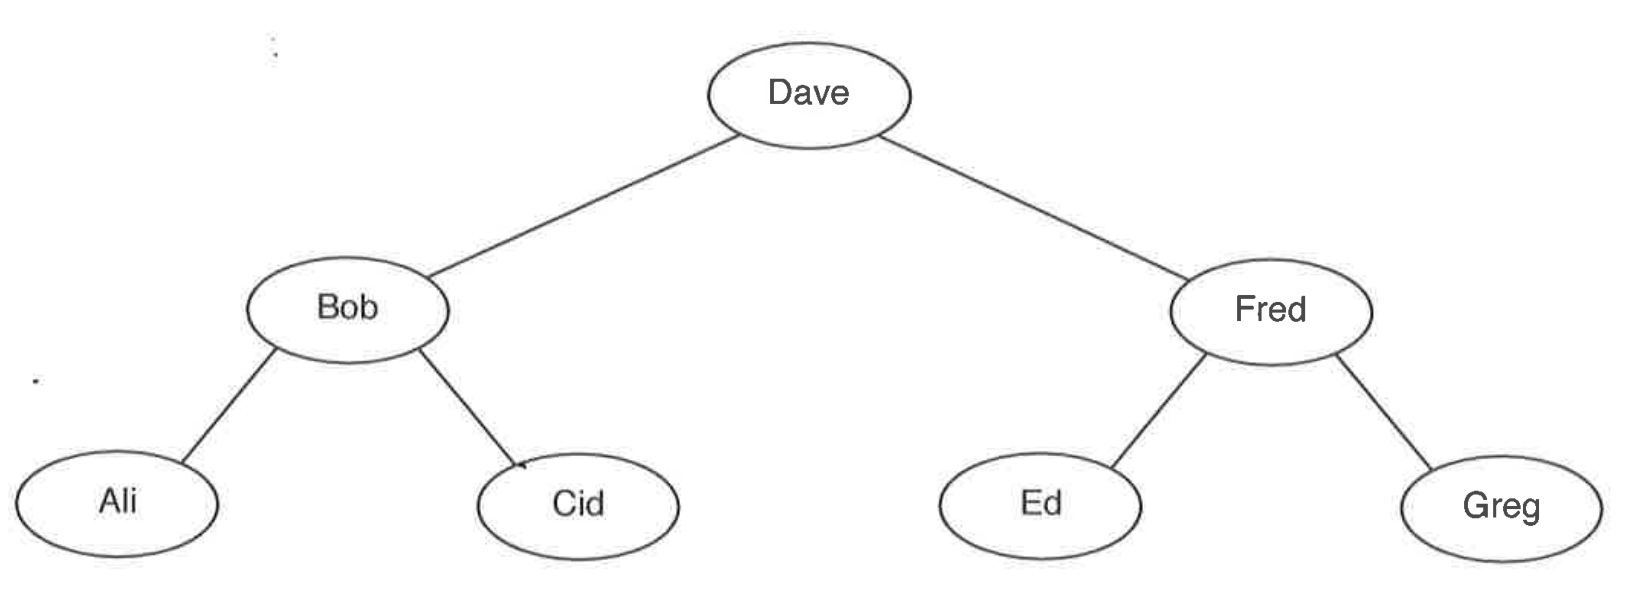
\includegraphics[width=0.5\paperwidth]{C:/Users/Admin/Desktop/Github/question_bank/static/img/9597-ALVL-2016-P1-Q3}
\par\end{center}

The program to implement this ADT will use the classes \texttt{Tree}
and \texttt{Node} designed as follows:
\begin{center}
\begin{tabular}{|l|}
\hline 
\texttt{\hspace{0.25\columnwidth}Tree}\tabularnewline
\hline 
\texttt{tree : ARRAY OF Node}\tabularnewline
\texttt{root : INTEGER}\tabularnewline
\tabularnewline
\hline 
\texttt{constructor()}\tabularnewline
\texttt{add(newItem)}\tabularnewline
\texttt{print() }\tabularnewline
\tabularnewline
\tabularnewline
\tabularnewline
\tabularnewline
\tabularnewline
\hline 
\end{tabular}%
\begin{tabular}{|l|}
\hline 
\hspace{0.25\columnwidth}\texttt{Node}\tabularnewline
\hline 
\texttt{data : STRING}\tabularnewline
\texttt{leftPtr : INTEGER}\tabularnewline
\texttt{rightPtr : INTEGER}\tabularnewline
\hline 
\texttt{constructor()}\tabularnewline
\texttt{setData(s : STRING)}\tabularnewline
\texttt{setLeftPtr(x : INTEGER)}\tabularnewline
\texttt{setRightPtr(y : INTEGER)}\tabularnewline
\texttt{getData() : STRING}\tabularnewline
\texttt{summary() : STRING}\tabularnewline
\texttt{getLeftPtr() : INTEGER}\tabularnewline
\texttt{getRightPtr() : INTEGER}\tabularnewline
\hline 
\end{tabular}
\par\end{center}

The program code must:
\begin{itemize}
\item Create a new tree, which has: 
\begin{itemize}
\item no nodes 
\item the root set to -1 
\end{itemize}
\item Use the root as a pointer to the first node in the tree 
\item Add a new node to the tree in the appropriate position 
\item Use the \texttt{print()} method to output, for each node, in array
order: 
\begin{itemize}
\item the data item 
\item the left pointer 
\item the right pointer. 
\end{itemize}
\end{itemize}

\subsubsection*{Task 3.1}

Write program code to define the classes \texttt{Tree} and \texttt{Node}. 

\subsubsection*{Evidence 6}

Your program code. \hfill{}{[}30{]}

\subsubsection*{Task 3.2}

The program is to be tested. 

Write a sequence of program statements to: 
\begin{itemize}
\item Create a tree 
\item Add the data items shown in the original list of ADT commands 
\item Print the array contents. 
\end{itemize}
Execute your program to test it. 

\subsubsection*{Evidence 7}

Your program code. 

Screenshot of test run.\hfill{} {[}3{]}

\subsubsection*{Task 3.3}

A method \texttt{inOrderTraversal()} is to be added, which outputs
the data stored in the tree in alphabetical order. 

Write program code to: 
\begin{itemize}
\item Implement this method 
\item Test the program code with the data from Task 3.2. 
\end{itemize}

\subsubsection*{Evidence 8}

Your program code. 

Screenshot of test run. \hfill{}{[}7{]}

 \newpage 

\item \textbf{{[}ALVL/9597/2016/P1/Q4{]} }

Numbers in Computing are often represented in hexadecimal form. 

A program is required to convert a hexadecimal number into a denary
number and vice versa. 

\subsubsection*{Task 4.1}

Write program code with the following specification: .
\begin{itemize}
\item Input a hexadecimal number as a string 
\item Validate the input 
\item Calculate the denary value of each hexadecimal digit (write this code
as a function)
\item Calculate the denary value of the hexadecimal number input
\item Output the denary value. 
\end{itemize}

\subsubsection*{Evidence 9}

Your program code. \hfill{}{[}10{]}

\subsubsection*{Task 4.2}

Draw up a list of \textbf{three} suitable test cases. Complete a table
with the following headings: 
\begin{center}
\begin{tabular}{|l|l|l|}
\hline 
Hexadecimal Number & Purpose of the test & Expected output\tabularnewline
\hline 
 &  & \tabularnewline
\hline 
 &  & \tabularnewline
\hline 
 &  & \tabularnewline
\hline 
\end{tabular}
\par\end{center}

Provide screenshot evidence for your testing. 

\subsubsection*{Evidence 10}

The completed table. 

Screenshots for each test data run. \hfill{}{[}5{]} 

\subsubsection*{Task 4.3}

Write additional code to convert a denary number into a hexadecimal
number. 

\subsubsection*{Evidence 11}

Your program code. \hfill{}{[}10{]}

\subsubsection*{Task 4.4}

Draw up a list of\textbf{ three} suitable test cases. Complete a table
with the following headings:
\begin{center}
\begin{tabular}{|l|l|l|}
\hline 
Denary Number & Purpose of the test & Expected output\tabularnewline
\hline 
 &  & \tabularnewline
\hline 
 &  & \tabularnewline
\hline 
 &  & \tabularnewline
\hline 
\end{tabular}
\par\end{center}

Provide screenshot evidence for your testing.

\subsubsection*{Evidence 12}

The completed table.

Screenshots for each test data run. \hfill{}{[}5{]}

 \newpage 

\item \textbf{{[}ALVL/9597/2016/P2/Q1{]} }

Many elderly people spend later life in a nursing home. The Ministry
of Health (MOH) requires each nursing home to keep detailed care records
for each resident. Care staff make daily entries in the care records
about all aspects of resident care. These care records are currently
paper-based documents. There is no common format for the documents
that different nursing homes use. 

Care staff do not have computer access to medical records that each
resident\textquoteleft s doctor holds. Nurses at a nursing home need
to keep their own medical records and to consult with residents\textquoteleft{}
doctors.

The MOH is planning an initiative to computerise all care records
and would like all nursing homes to use a common design for care records.

The MOH will send a project proposal which is to be circulated to
all nursing homes. This is to find out which homes would consider
taking part in a pilot project. The MOH's aim is to introduce a pilot
system into a single nursing home.

The MOH needs to find a software house to design and implement the
computerised care record system. It will send the project proposal
to software houses.

At a later date, all nursing homes will use the new computer system.
\begin{enumerate}
\item {} 
\begin{enumerate}
\item State \textbf{four} topics you would expect to find in this project
proposal.\hfill{} {[}4{]}
\item Describe the purpose of this project proposal. \hfill{}{[}2{]}
\end{enumerate}
Following production of the project proposal. the initial activities
with their expected times are as follows:
\begin{center}
\begin{tabular}{|c|>{\raggedright}p{0.5\columnwidth}|c|}
\hline 
\textbf{Label} & \texttt{\textbf{\hspace{0.01\columnwidth}}}\textbf{Activity } & \textbf{Time (weeks)}\tabularnewline
\hline 
A & Send the project proposal document to all nursing homes. & 5\tabularnewline
\hline 
B & Circulate the project proposal document to a number of software houses. & 6\tabularnewline
\hline 
C & Review the feedback. Note which nursing homes and software houses
have expressed interest.  & 2\tabularnewline
\hline 
D & identify doctors who look after residents in homes that have expressed
interest. Hold a presentation meeting to explain the proposed project
to these doctors. & 5\tabularnewline
\hline 
E & Presentation event for the chosen nursing home. & 2\tabularnewline
\hline 
\end{tabular}
\par\end{center}

\end{enumerate}
The Program Evaluation and Review Technique (PERT) chart for these
initial activities is shown below. 
\begin{center}
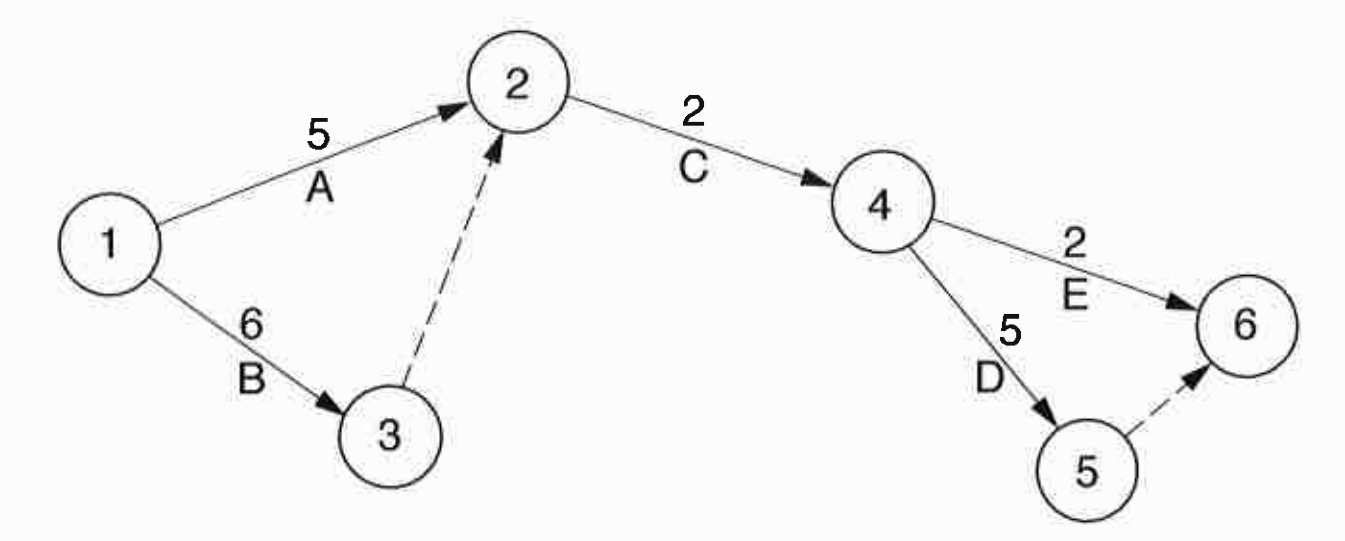
\includegraphics[width=0.5\paperwidth]{C:/Users/Admin/Desktop/Github/question_bank/static/img/9597-ALVL-2016-P2-Q1-1}
\par\end{center}
\begin{enumerate}
\item[(b)] {}
\begin{enumerate}
\item State the critical path for the initial activities. \hfill{}{[}1{]}
\item Calculate the minimum time these initial activities will take.\hfill{}
{[}1{]}
\end{enumerate}
\item[(c)] In activity E, the MOH presented more details about the project to
the manager and care staff of the chosen nursing home. The manager
and care staff raised a number of points about both social and ethical
issues associated with the project. 

Describe \textbf{three} points that could have been raised.\hfill{}
{[}6{]}
\end{enumerate}
Following activity E, the MOH decided the software house to which
it would award the contract. 

Following the initial project proposal. activities which make up the
system development cycle are shown below:
\begin{center}
\begin{tabular}{|c|>{\raggedright}p{0.5\columnwidth}|c|}
\hline 
\textbf{Label} & \texttt{\textbf{\hspace{0.01\columnwidth}}}\textbf{Activity} & \textbf{Time (weeks)}\tabularnewline
\hline 
F & Analysis & 12\tabularnewline
\hline 
G & Design & 15\tabularnewline
\hline 
H & Data entry of current care record data & 4\tabularnewline
\hline 
I & Initial testing & 10\tabularnewline
\hline 
J & Program development  & 14\tabularnewline
\hline 
K & Install new hardware in nursing home  & 3\tabularnewline
\hline 
L & Alpha testing & 2\tabularnewline
\hline 
M & Beta testing & 1\tabularnewline
\hline 
N & Implementation & 3\tabularnewline
\hline 
\end{tabular}
\par\end{center}

\begin{center}
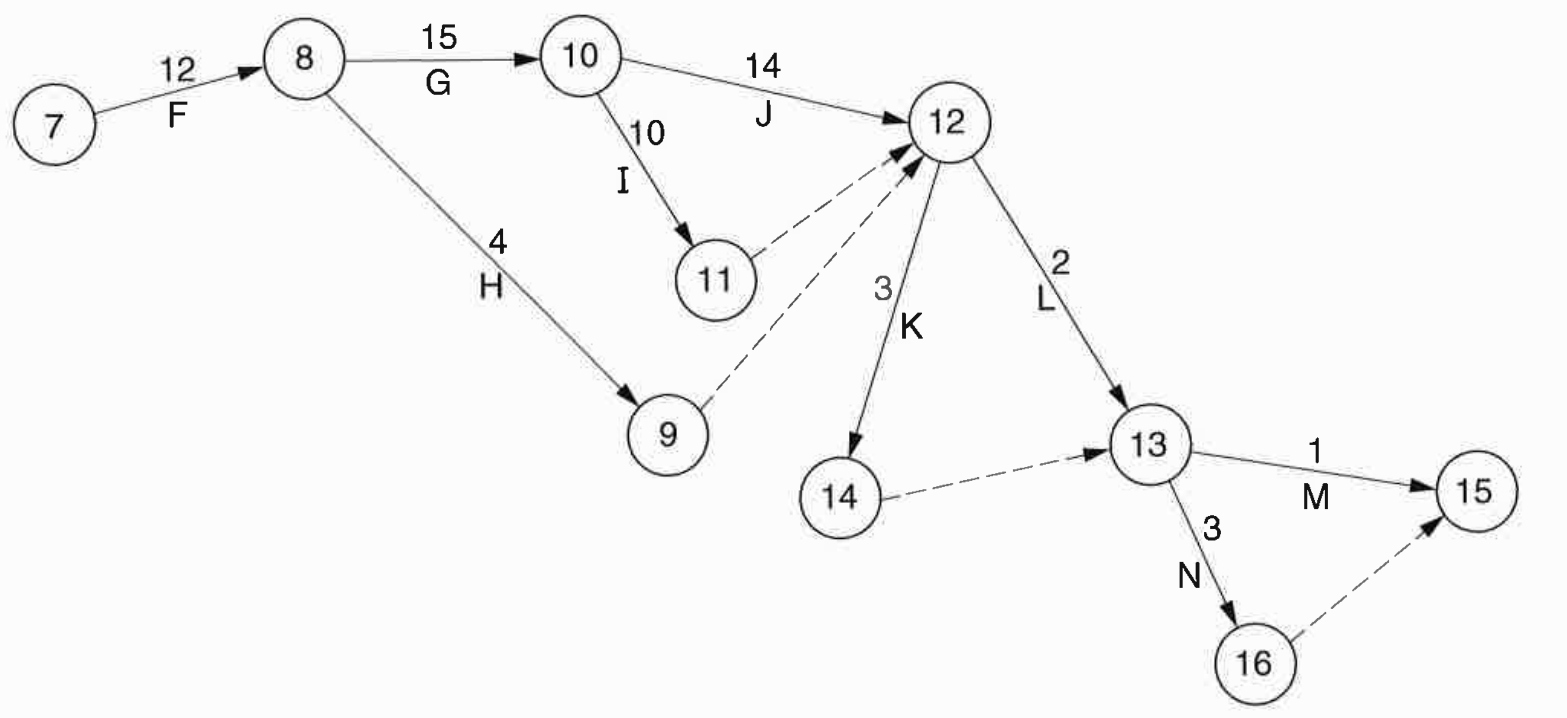
\includegraphics[width=0.5\paperwidth]{C:/Users/Admin/Desktop/Github/question_bank/static/img/9597-ALVL-2016-P2-Q1-2}
\par\end{center}
\begin{enumerate}
\item[(d)] The system development cycle starts at node (time point) 7.
\begin{enumerate}
\item The PERT chart shows four activities with dashed lines. Explain the
significance of the dashed lines.\hfill{} {[}1{]}
\item Explain the meanings of a dependent stage and concurrent stages in
a PERT chart. Give an example of each for this project. \hfill{}{[}4{]}
\item The table describes activity I as \textquoteleft initial testing'.
One category of initial testing is white-box testing.

Name and describe two other categories of initial testing. \hfill{}{[}4{]}
\item The PERT chart indicates that some testing can commence almost as
soon as program development does. Describe the type of program development
that would allow for this.\hfill{} {[}2{]}
\end{enumerate}
\item[(e)] An analyst from the software house carried out the analysis for the
project. 

Describe \textbf{three} examples of people whom the analyst consulted.
For each example. state: 
\begin{itemize}
\item the fact finding technique used 
\item the nature of the information that the analyst obtained. 
\end{itemize}
Each fact finding technique should be different.\hfill{} {[}6{]}
\item[(f)]  When the analysis stage was completed. the following decisions were
taken: 
\begin{itemize}
\item Each nursing home will store and manage its own care records data. 
\item Each nursing home will be provided with a local area network (LAN). 
\item The care record system on each LAN will use a client-server model
with a web interface for client computers. 
\end{itemize}
\begin{enumerate}
\item Explain the meaning of the term client-server model. \hfill{}{[}3{]}
\item State the \textbf{two} items of software that the LAN will use to
implement this client-server design. \hfill{}{[}2{]}
\end{enumerate}
\end{enumerate}
During the presentation event to doctors (part of activity D). the
doctors gave feedback. They said that they would like to have access
to the new computerised care records from their own offices. 
\begin{enumerate}
\item[(g)] A second phase of the project is to allow each nursing home access
to the medical data stored by doctors. This will involve connecting
the LAN for each nursing home to a number of doctors' surgery LANs. 
\begin{enumerate}
\item (l) State \textbf{two} methods for ensuring the security of access
to the care record network application. \hfill{}{[}2{]}
\item (ll) Give \textbf{two} methods for protecting the security of the
LAN. \hfill{}{[}2{]}
\end{enumerate}
\end{enumerate}

 \newpage 

\item \textbf{{[}ALVL/9597/2016/P2/Q2{]} }

A firm hires vehicles to customers. A customer usually makes a booking
a number of weeks before the start of the hire period. The customer
pays a deposit at the time of the booking and the balance when they
return the vehicle from hire.

At the time of the booking, the firm records the following data:
\begin{itemize}
\item customer data, including a customer reference code
\item booking date
\item hire start date
\item hire return date
\item type of vehicle
\item deposit taken
\end{itemize}
Vehicle types are coded as follows:
\begin{itemize}
\item Small car - SC
\item Large car - LC
\item Utility vehicle - UV
\end{itemize}
Each vehicle type has its own daily charge, for each day of the hire
period.

Each vehicle has a unique registration.

Customers may make more than one booking. The software will not allow
a customer to make more than one booking for the same start date.

The document below is an example of an invoice printed for the customer
when they return the vehicle and pay the balance due.
\begin{center}
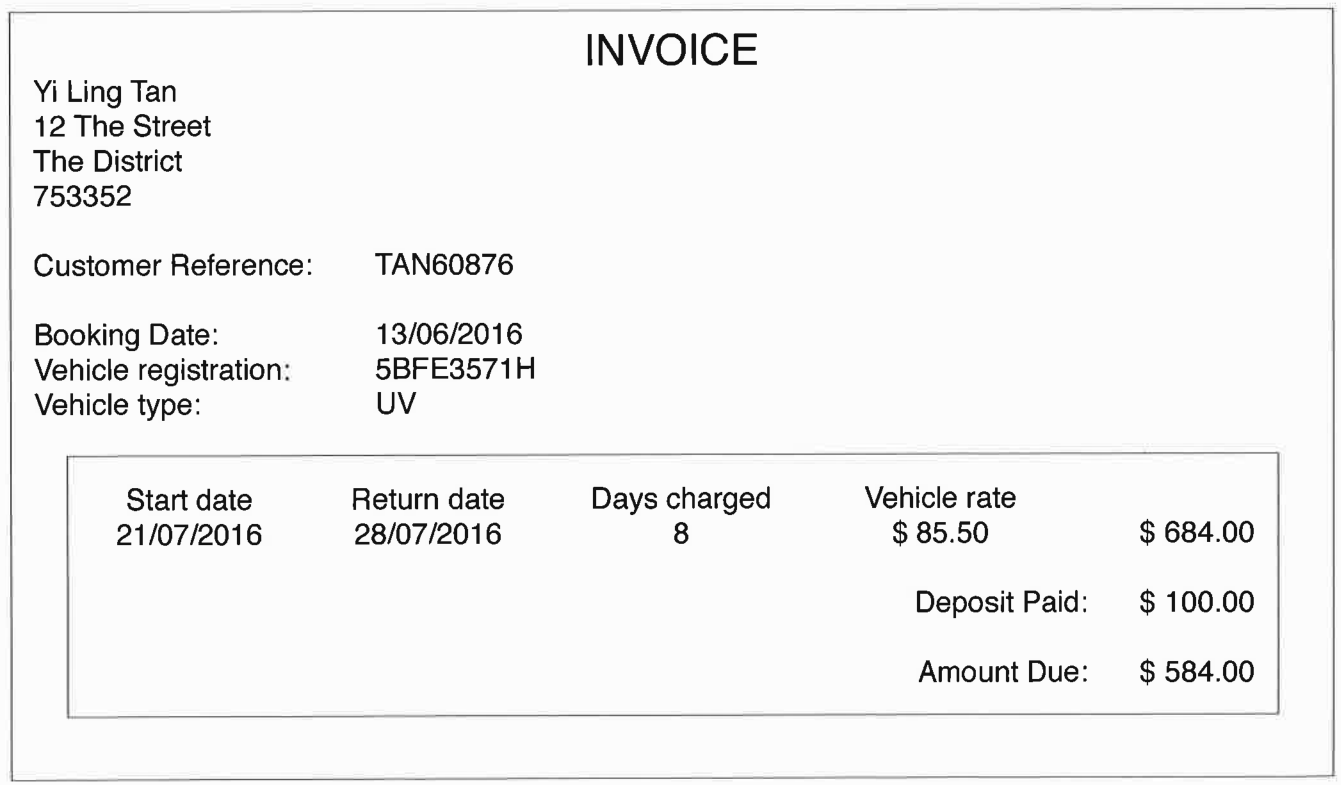
\includegraphics[width=0.5\paperwidth]{C:/Users/Admin/Desktop/Github/question_bank/static/img/9597-ALVL-2016-P2-Q2}
\par\end{center}
\begin{enumerate}
\item The firm wants to model this application using a relational database.
\begin{enumerate}
\item A database needs a number of tables to store the data for this application.
Draw the Entity-Relationship (E-R) diagram showing the tables and
the relationships between them. \hfill{}{[}6{]}
\item A table description can be expressed as: 

\texttt{TableName (}\texttt{\uline{Attributel}}\texttt{ , Attribute2
, Attribute3 , ....) }

The primary key is indicated by underlining one or more attributes. 

Write table descriptions for the tables you identified in \textbf{part
(i)}. \hfill{}{[}6{]}
\end{enumerate}
\item The firm implements the relational database using a Database Management
System (DBMS). It writes programs to access the data using a Graphical
User Interface (GUI). 

One program is for recording a new booking. 

The firm uses different types of components in a GUI for the display
and entry of data. 

Name \textbf{three} types of component that the booking form could
use and give the types of data it is used to capture. \hfill{} {[}3{]}
\end{enumerate}

 \newpage 

\item \textbf{{[}ALVL/9597/2016/P2/Q3{]} }

The recursive procedure \texttt{X} was two parameters, \texttt{Value}
and \texttt{Index}. The procedure processes the contents of an array,
\texttt{T}.

\noindent %
\noindent\begin{minipage}[t]{1\columnwidth}%
\texttt{01 PROCEDURE X(Value, Index)}

\texttt{02 \qquad{}IF T{[}Index{]} > 0}

\texttt{03 \qquad{}\qquad{}THEN}

\texttt{04 \qquad{}\qquad{}\qquad{}IF T{[}Index{]} > Value}

\texttt{05 \qquad{}\qquad{}\qquad{}\qquad{}THEN}

\texttt{06 \qquad{}\qquad{}\qquad{}\qquad{}\qquad{}X(Value, Index
{*} 2) }

\texttt{07 \qquad{}\qquad{}\qquad{}ENDIF}

\texttt{08 \qquad{}\qquad{}\qquad{}IF T{[}Index{]} < Value}

\texttt{09 \qquad{}\qquad{}\qquad{}\qquad{}THEN}

\texttt{10 \qquad{}\qquad{}\qquad{}\qquad{}\qquad{}X(Value, Index
{*} 2 + 1) }

\texttt{11 \qquad{}\qquad{}\qquad{}ENDIF}

\texttt{12 \qquad{}\qquad{}\qquad{}IF T{[}Index{]} = Value}

\texttt{13 \qquad{}\qquad{}\qquad{}\qquad{}THEN}

\texttt{14 \qquad{}\qquad{}\qquad{}\qquad{}\qquad{}OUTPUT \textquotedbl True\textquotedbl}

\texttt{15 \qquad{}\qquad{}\qquad{}ENDIF}

\texttt{l6 \qquad{}ENDIF}

\texttt{17 ENDPROCEDURE}%
\end{minipage}
\begin{enumerate}
\item {}
\begin{enumerate}
\item State what is meant by a recursive procedure. \hfill{}{[}1{]}
\item Give the two line numbers which indicate that procedure x is recursive.
\hfill{} {[}1{]}
\end{enumerate}
\item An array T is used to store the data for a binary tree. A program
places items in the array in the order in which they joined the tree
structure. 
\begin{center}
\begin{tabular}{|c|c|c|c|c|c|c|c|c|c|c|c|c|c|c|}
\hline 
1 & 2 & 3 & 4 & 5 & 6 & 7 & 8 & 9 & 10 & 11 & 12 & 13 & 14 & 15\tabularnewline
\hline 
17 & 11 & 19 & 9 & 12 & 18 & 23 & 0 & 4 & 0 & 0 & 0 & 0 & 0 & 0\tabularnewline
\hline 
\end{tabular}
\par\end{center}
\begin{enumerate}
\item Draw the binary tree for the array \texttt{T} dataset. \hfill{} {[}3{]}
\item Copy and then complete the trace table for the procedure call \texttt{X(18,
1)}.
\begin{center}
\begin{tabular}{|c|c|c|c|}
\hline 
Procedure call & \texttt{Value} & \texttt{Index} & Output\tabularnewline
\hline 
\texttt{1} & \texttt{18} & \texttt{1} & \tabularnewline
\hline 
 &  &  & \tabularnewline
\hline 
 &  &  & \tabularnewline
\hline 
 &  &  & \tabularnewline
\hline 
 &  &  & \tabularnewline
\hline 
\end{tabular} 
\par\end{center}

\begin{center}
\hfill{}{[}3{]}
\par\end{center}
\item Describe the purpose of procedure \texttt{X}. \hfill{}{[}2{]}
\end{enumerate}
\end{enumerate}

 \newpage 

\item \textbf{{[}ALVL/9597/2016/P2/Q4{]} }

Data is to be transmitted in packets between two computers. 

Each packet message can consist of: 
\begin{itemize}
\item upper case letters 
\item the <Space> character. 
\end{itemize}
Each packet has a start character (\#) and an end character (\#). 

A typical packet would be: 
\begin{center}
\texttt{\#ETA FROM SRE\#}
\par\end{center}
\begin{enumerate}
\item Describe\textbf{ two} checks that the receiving computer should make
for the integrity of:
\begin{itemize}
\item the individual bytes which make up a packet
\item the collection of bytes which makes up the packet. \hfill{} {[}4{]}
\end{itemize}
\item Describe \textbf{three} validation checks that the receiving computer
should pertorm on the packet. \hfill{}{[}6{]}
\end{enumerate}

 \newpage 

\item \textbf{{[}ALVL/9597/2016/P2/Q5{]} }

A programmer implements a linked list of surnames with a start pointer,
\texttt{StartPtr} and two one-dimensional arrays: 
\begin{itemize}
\item Array \texttt{Data} stores the surnames. 
\item Array \texttt{Ptr} stores the link pointers.
\item Both arrays have lower bound 1 and upper bound 3000. 
\end{itemize}
The purpose of procedure \texttt{InsertListItem} is to insert a new
surname to the linked list. 

Assume a function \texttt{NextFree()} is available and returns: 
\begin{itemize}
\item the index position for the array \texttt{Data} at which the new surname
is to be inserted 
\item -1 when the \texttt{Data} array is full. 
\end{itemize}
The programmer designs the algorithm as follows:

\noindent %
\noindent\begin{minipage}[t]{1\columnwidth}%
\texttt{01 PROCEDURE InsertListItem(NewSurname : STRING) }

\texttt{02 \qquad{}IF NextFree() = \textemdash 1 }

\texttt{03 \qquad{}\qquad{}THEN }

\texttt{04 \qquad{}\qquad{}\qquad{}OUTPUT \textquotedbl List is
full\textquotedbl{} }

\texttt{05 \qquad{}\qquad{}ELSE }

\texttt{O6 \qquad{}\qquad{}\qquad{}// input the surname }

\texttt{07 \qquad{}\qquad{}\qquad{}IF StartPtr = 0 }

\texttt{08 \qquad{}\qquad{}\qquad{}\qquad{}THEN }

\texttt{09 \qquad{}\qquad{}\qquad{}\qquad{}\qquad{}StartPtr w
NextFree() }

\texttt{10 \qquad{}\qquad{}\qquad{}\qquad{}\qquad{}Data{[}StartPtr{]}
e NewSurname }

\texttt{11 \qquad{}\qquad{}\qquad{}\qquad{}ELSE }

\texttt{12 \qquad{}\qquad{}\qquad{}\qquad{}\qquad{}// traverse
the linked list to find the position }

\texttt{13 \qquad{}\qquad{}\qquad{}\qquad{}\qquad{}// at which
to insert NewSurname}

$\vdots$

\texttt{\qquad{}\qquad{}\qquad{}\qquad{}ENDIF }

\texttt{\qquad{}\qquad{}ENDIF }

\texttt{\qquad{}ENDPROCEDURE}%
\end{minipage}
\begin{enumerate}
\item Describe the state of the linked list. if the condition \texttt{StartPtr
= 0} in line \texttt{07} is \texttt{True}. {[}1{]} 
\item It is now necessary to complete the design for procedure \texttt{InsertListItem}. 
\begin{enumerate}
\item The pseudocode already uses some variables. 

Copy the table below and complete it to show any extra variables that
you will need to use. 
\begin{center}
\begin{tabular}{|c|c|c|}
\hline 
\textbf{Variable} & \textbf{Data Type} & \textbf{Description}\tabularnewline
\hline 
 &  & \tabularnewline
\hline 
 &  & \tabularnewline
\hline 
 &  & \tabularnewline
\hline 
 &  & \tabularnewline
\hline 
 &  & \tabularnewline
\hline 
\end{tabular}
\par\end{center}

\hfill{}{[}3{]}
\item Write the pseudocode for line \texttt{14} onwards to complete the
procedure. \hfill{}{[}6{]}
\end{enumerate}
\end{enumerate}

 \newpage 

\item \textbf{{[}ALVL/9597/2016/P2/Q6{]} }

A real-estate management company owns a number of residential and
business units. When the company first acquires a unit, it often requires
renovation work. The company records the renovation cost.

A residential unit will be a house or an individual flat within a
building. A business unit will be either an office building, a storage
unit or a factory.

A residential unit is either advertised for sale, with the company
looking to make a profit, or retained for rental. If the unit is sold,
the sale price is recorded. If the unit is retained, the monthly rental
charged, the start date and length of the rental (in months) are recorded.

A business unit has a long term lease, which is usually 10 years or
longer. The company records the nature of the business. it does not
offer any of its business units for sale. 

Other data recorded for a unit include: purchase price, purchase date,
number of rooms, floor space, whether or not a lift is present. The
company records whether the house has a garage and whether it has
a garden. 

A programmer will develop an application, using object-oriented programming
to store and process the company\textquoteright s data. 
\begin{enumerate}
\item Draw a class diagram, with base class \texttt{UNIT}, showing: 
\begin{itemize}
\item appropriate sub-class(es)
\item inheritance 
\item the properties required 
\item appropriate methods, including \textbf{one} pair of \textquoteleft get\textquoteright{}
and \textquoteleft set\textquoteleft{} methods for \textbf{one} of
the properties.\hfill{} {[}8{]}
\end{itemize}
\item The company has recently purchased a number of units that they want
to renovate as a \textquoteleft block of flats\textquoteright{} (a
number of self-contained flats in the same building). Once the renovation
is complete, the company may offer a block of flats for sale. Alternatively,
it may retain the unit and advertise each individual flat for rental. 

Explain how this would affect the design in \textbf{part (a)}. \hfill{}{[}3{]}
\item {}
\begin{enumerate}
\item Explain the meaning of the term encapsulation. \hfill{}{[}2{]}
\item Explain the meaning of the term polymorphism. \hfill{}{[}2{]}
\end{enumerate}
\end{enumerate}

 \newpage 

\item \textbf{{[}DHS/PRELIM/9597/2016/P1/Q1{]} }

In Olympic diving, scoring is done by a panel comprising a minimum
of 3 judges. The highest and lowest scores are dropped to eliminate
the extremes. The raw score is computed by summing the middle scores.
The raw score is then multiplied by the level of difficulty to give
the total score. 

Sample scoring for a 5-judges panel: Scores: 

6.5, 6, 6.5, 6, 5.5 

Lowest (5.5) and highest (6.5) scores dropped 

Raw Score = 18.5 (6.5 + 6 + 6) 

Total Score = Score (18.5) x Difficulty Level (1.5) = 27.75 

\texttt{DIVE1.TXT} contains the countries, difficulty levels and 5-judges
scores for a diving competition. 

\subsection*{Task 1.1 }

Write program code to determine the podium winners of the competition.
Your program should output the medal (Gold, Silver, Bronze), country
name and the total score (to 2 decimal places). 

Sample output:

\noindent %
\noindent\begin{minipage}[t]{1\columnwidth}%
\texttt{Gold: China 45.90 }

\texttt{Silver: Malaysia 39.20}

\texttt{Bronze: United States 36.00 }%
\end{minipage}

\subsection*{Evidence 1: }

Program code. \hfill{}{[}5{]}

\subsection*{Evidence 2: }

Screenshot of output. \hfill{}{[}1{]}

In most international competitions with more than five judges, the
3/5 method is used. The middle 5 numbers are added and then multiplied
by the difficulty of the dive and then multiplied again by 0.6. \texttt{DIVE2.TXT}
contains the countries, difficulty levels and 9-judges scores for
a diving competition. 

\subsection*{Task 1.2 }

Write program code to determine the podium winners of the competition.
Your program should output the medal (Gold, Silver, Bronze), country
name as well as the total score (to 2 decimal places). 

\subsection*{Evidence 3: }

Program code. \hfill{}{[}8{]}

\subsection*{Evidence 4: }

Screenshot of output. \hfill{}{[}1{]}

 \newpage 

\item \textbf{{[}DHS/PRELIM/9597/2016/P1/Q2{]} }

Quicksort is an efficient sorting algorithm to order values in an
array. 

\subsection*{Task 2.1 }

Write a recursive quicksort method to sort the values in the text
file \texttt{DATA.TXT} in descending order. 

\subsection*{Evidence 5: }

Program code for Task 2.1. \hfill{}{[}4{]}

\subsection*{Evidence 6:}

Screenshot of output. \hfill{}{[}2{]}

\subsection*{Task 2.2 }

Using a suitable data structure, convert the recursive quicksort in
Task 2.1 to one using iteration. Confirm the correctness of your iterative
quicksort on the data set used in Task 2.1 

\subsection*{Evidence 7:}

Program code for Task 2.2.\hfill{}{[}8{]}

\subsection*{Evidence 8: }

Screenshot of output. \hfill{}{[}1{]}

 \newpage 

\item \textbf{{[}DHS/PRELIM/9597/2016/P1/Q3{]} }

A Pokemon Go fan who nicknames himself Pokeboy wishes to manage his
Pokemon collection using a binary search tree. Each binary search
tree node stores the name together with the numbers of that particular
Pokemon and candies collected, as well as a reference to a linked
list. Each linked list node stores the combat power (CP) of a Pokemon.
The binary search tree is organised in ascending Pokemon name order.
Each linked list is organised in descending order of CP. For ease
of reference, we shall name this composite data structure Poketree. 

\subsection*{Task 3.1 }

Using object-oriented programming, construct appropriate classes to
initialise, insert and display the contents of the Poketree. In your
main driver program, write code to initialise a Poketree with the
first Pokemon collected which is randomly generated from the contents
in the file \texttt{POKEMONS.TXT} as well as a randomly generated
CP in the range 10 to 200 inclusive. When a Pokemon is caught, 3 candies
of that kind are also added to the candies count of the Poketree binary
search tree node.

\subsection*{Evidence 9: }

Program code for class definition, initialisation and display methods.\hfill{}
{[}7{]}

\subsection*{Evidence 10:}

Screenshot output to show contents of Poketree with first Pokemon
inserted.\hfill{} {[}1{]}

\subsection*{Task 3.2 }

Write a class method \texttt{insert()} and the necessary main driver
program code to insert another 23 randomly generated Pokemons and
their corresponding CPs into the Poketree. 

\subsection*{Evidence 11: }

Program code for Task 3.2.\hfill{} {[}4{]}

\subsection*{Evidence 12:}

Screenshot to show updated contents of Poketree.\hfill{} {[}1{]}

Apart from collecting Pokemons, one can also evolve Pokemons. When
a new Pokemon is evolved, its previous incarnation is deleted from
the Poketree and its new incarnation either inserted (if its kind
is not previously collected) or updated (if its kind is previously
collected) to the Poketree. Evolving also requires a set amount and
type of Pokemon candy. If there is insufficient Pokemon candies, Pokeboy's
preferred action is to exchange (i.e. delete) existing Pokemons of
the same species for candies, starting from the Pokemon with the lowest
CP. Each Pokemon can be exchanged for one candy. Pokeboy also wishes
to keep at least 2 Pokemons of the same species in his collection
(well he is a Pokemon fan). The text file \texttt{CANDIES.TXT} contains
the candies requirement for evolvement. 

\subsection*{Task 3.3 }

Write a Boolean class method \texttt{can\_evolve(pokemon)} to determine
if a particular Pokemon can evolve by Pokeboy's preference. A Pokemon
can evolve if there are sufficient candies or it is possible to exchange
candies, leaving a minimum of 2 Pokemons of that species.

Write a class method evolve(pokemon) which will evolve a Pokemon using
\texttt{can\_evolve(pokemon)}. 

Add necessary class method(s) and main driver program code to evolve
all evolvable Pokemons. 

\subsection*{Evidence 13: }

Program code for Task 3.3.\hfill{} {[}7{]}

\subsection*{Evidence 14:}

Screenshot(s) to show evolution.\hfill{} {[}1{]}

\subsection*{Task 3.4 }

Write a class method \texttt{most\_poke()} to output the frequency
and most collected Pokemon(s) collected by Pokeboy. 

Add necessary program code to exercise \texttt{most\_poke()}.

\subsection*{Evidence 15: }

Program code for Task 3.4.\hfill{} {[}4{]}

\subsection*{Evidence 16:}

Screenshot for Task 3.4. \hfill{}{[}1{]}

\subsection*{Task 3.5}

Pokeboy aspires to join the Catch Them All club. The Catch Them All
club is a group of elites who have managed to catch every species
of Pokemon at least once. Write a class method \texttt{catch\_them\_all()}
to either output the message \textquotedbl Welcome to the club! You
have caught them all!\textquotedbl{} or output the number and remaining
Pokemon names yet to be caught.

Add necessary program code to exercise \texttt{catch\_them\_all()}. 

\subsection*{Evidence 17:}

Program code for Task 3.5.\hfill{} {[}6{]}

\subsection*{Evidence 18: }

Screenshot for annotated test cases. \hfill{}{[}2{]}

\subsection*{Task 3.6 }

After some time, it becomes necessary to reorganise the binary search
tree to ensure optimal search performance. Write program code to rebalance
the binary search tree and include as comments your strategy to do
this. You should output the roots and heights of the old and new binary
search trees.

\subsection*{Evidence 19:}

Program code for Task 3.6.\hfill{} {[}5{]}

\subsection*{Evidence 20:}

Screenshot.\hfill{} {[}1{]}

 \newpage 

\item \textbf{{[}DHS/PRELIM/9597/2016/P1/Q4{]} }

A magic index in an array A is defined to be an index such that \texttt{A{[}i{]}
= i}. 

\subsection*{Task 4.1 }

Given a sorted array of distinct integers, write a brute force iterative
method \texttt{magic\_index(A)} to find a magic index if one exists.
If a magic index does not exist, return -1. 

\subsection*{Evidence 21: }

Function code for \texttt{magic\_index(A)} and relevant driver code.\hfill{}
{[}5{]}

\subsection*{Evidence 22: }

Screenshot of output.\hfill{} {[}2{]}

\subsection*{Task 4.2 }

Write an efficient recursive method \texttt{magic\_index\_duplicates(A)}
to find a magic index for an array containing non-distinct values.
If a magic index does not exist, return -1.

\subsection*{Evidence 23: }

Function code for \texttt{magic\_index\_duplicates(A)} and relevant
driver code. \hfill{} {[}6{]}

\subsection*{Evidence 24:}

Screenshot of output. \hfill{} {[}2{]}

A child is running up a staircase with n steps and can hop either
1, 2 or 3 steps at a time. 

\subsection*{Task 4.3 }

Write a brute force recursive method to count how many possible ways
the child can run up the stairs. 

\subsection*{Evidence 25: }

Function code and relevant driver code.\hfill{} {[}5{]}

\subsection*{Evidence 26: }

Screenshot of output.\hfill{} {[}2{]}

\subsection*{Task 4.4 }

Optimise your brute force recursive solution in Task 4.3 by eliminating
unnecessary recomputations.

\subsection*{Evidence 27: }

Function code and relevant driver code.\hfill{} {[}6{]}

\subsection*{Evidence 28:}

Screenshots showing annotated test cases. \hfill{} {[}2{]}

 \newpage 

\item \textbf{{[}DHS/PRELIM/9597/2016/P2/Q1{]} }

GovBuy is a Government Digital Services initiative that helps government
employees buy microservices (small pieces of software that can be
deployed independently), software libraries, non-critical bug fixes
or even customised hardware from independent contractors. 

The platform allows government employees to post a task. Anyone can
bid to take on the task during the bidding period. The reverse auction
starts at \$5,000 and the lowest bid wins.

The winner works on the task and submits completed code to the team.
If the code meets the acceptance criteria before the deadline, the
winner is sent a cheque for the work.

The current prototype platform is a web interface:
\begin{center}
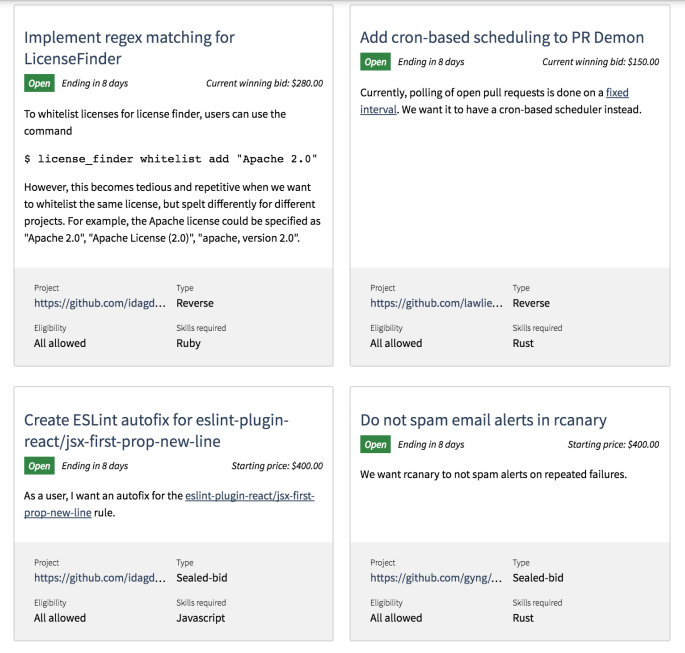
\includegraphics[width=0.5\paperwidth]{C:/Users/Admin/Desktop/Github/question_bank/LyX/static/img/9597-DHS-2016-P2-Q1-1}
\par\end{center}
\begin{enumerate}
\item The agency in charge wishes to develop mobile native versions of the
platform for Android and iOS. The following diagram shows the expected
workflow. 
\begin{center}
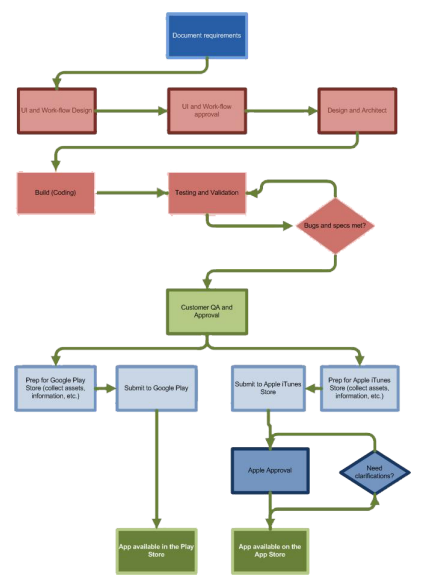
\includegraphics[width=0.5\paperwidth]{C:/Users/Admin/Desktop/Github/question_bank/LyX/static/img/9597-DHS-2016-P2-Q1-2}
\par\end{center}
\begin{enumerate}
\item Create a PERT chart from the above workflow diagram. You may assume
the following durations from the activity table below.\hfill{} {[}4{]}
\noindent \begin{center}
\begin{tabular}{|c|l|c|}
\hline 
Phase & Description & Duration (weeks)\tabularnewline
\hline 
A & Gather and document requirements & 2\tabularnewline
\hline 
B & UI and workflow design and approval & 3\tabularnewline
\hline 
C & Design and architect & 4\tabularnewline
\hline 
D & Build (coding) & 7\tabularnewline
\hline 
E & Testing and validation & 3\tabularnewline
\hline 
F & Customer QA and approval & 2\tabularnewline
\hline 
G & Prepare and submit to Google Play Store & 1\tabularnewline
\hline 
H & Prepare and submit to Apple App Store & 1\tabularnewline
\hline 
I & Apple approval & 1\tabularnewline
\hline 
\end{tabular} 
\par\end{center}
\item From the PERT chart, state the critical path and the minimum project
completion time. \hfill{}{[}2{]}
\item Describe two benefits which can be gained by producing a PERT chart.\hfill{}
{[}2{]}
\item Describe and give an example of a dependent activity. \hfill{}{[}2{]}
\item Describe and give an example of a concurrent activity.\hfill{} {[}2{]}
\end{enumerate}
\item The project manager decides he needs another diagrammatic tool to
monitor the project progress.
\begin{enumerate}
\item Create a Gantt chart for the project.\hfill{} {[}3{]}
\item Explain how the Gantt chart can help the developers in carrying out
their work.\hfill{} {[}2{]}
\end{enumerate}
\item Describe two activities to mark the closure of the project. \hfill{}{[}4{]}
\item Cybersecurity is of paramount concern when it comes to government
web services. Using suitable examples, explain the following cybersecurity
exploits and suggest how they can be mitigated. 
\begin{enumerate}
\item Cross site scripting \hfill{}{[}3{]}
\item Code injection \hfill{}{[}3{]}
\item Denial of service attack \hfill{}{[}3{]}
\end{enumerate}
\item The platform will be hosted using cloud computing. 
\begin{enumerate}
\item Explain why the cloud is a suitable hosting platform. \hfill{}{[}2{]}
\item Use suitable example to illustrate the concepts of IaaS, PaaS and
SaaS. \hfill{}{[}6{]}
\end{enumerate}
\item What ethical considerations should bidders bear in mind when bidding
for tasks on an open source platform such as GitHub?\hfill{} {[}2{]}
\end{enumerate}

 \newpage 

\item \textbf{{[}DHS/PRELIM/9597/2016/P2/Q2{]} }

The current GovBuy prototype supports two types of reverse auctions:
a standard reverse auction and a sealed bid auction. 

A standard reverse auction is one where bids begin at \$5,000. The
lowest possible bid is \$1, and an auction automatically ends once
a \$1 bid has been submitted. Bidders are allowed to submit multiple
bids throughout the duration of the auction. Bidders will see whether
they are the winning bidder after submitting a bid, and will have
an opportunity to submit a lower bid if the auction is still running.
The GitHub user names of participating bidders are hidden during the
auction. At the end of the auction, all bidders' GitHub accounts and
bid amounts will be unsealed and posted on the GovBuy platform. A
sealed bid auction is a type of reverse auction. Each bidder is allowed
to submit only one bid in an auction. Once a bid is submitted, the
bidder may not submit a second bid for the same auction. The lowest
bidder at the conclusion of the auction will still win the auction.
In the event that one or more bidders have the same bid amount, the
bidder who was first to submit the lowest bid amount will win the
auction. All bids will stay sealed until the end of the auction. A
bidder will not know the amounts other bidders have bidded on the
auction, or how many bids have been submitted. At the end of the auction,
all bidders' GitHub accounts and bid amounts will be unsealed and
posted on the GovBuy platform. 
\begin{enumerate}
\item Illustrate the types of reverse auctions in a class UML diagram. \hfill{}{[}5{]}
\item Using your illustration, explain the following OOP concepts: 
\begin{enumerate}
\item encapsulation \hfill{}{[}2{]}
\item inheritance \hfill{}{[}2{]}
\item polymorphism \hfill{} {[}2{]}
\end{enumerate}
\end{enumerate}

 \newpage 

\item \textbf{{[}DHS/PRELIM/9597/2016/P2/Q3{]}}

The following code shows the program \texttt{mystery1}. 

\noindent %
\noindent\begin{minipage}[t]{1\columnwidth}%
\texttt{epsilon = 0.01 }

\texttt{step = epsilon {*}{*} 2}

\texttt{num\_guesses = 0}

\texttt{ans = 0.0 }

\texttt{while abs(ans {*}{*} 2 - x) >= epsilon and ans {*} ans <=
x: }

\texttt{\qquad{}ans += step }

\texttt{\qquad{}num\_guesses += 1 }

\texttt{print(\textquotedbl\#Guesses =\textquotedbl , num\_guesses) }

\texttt{print(\textquotedbl Answer =\textquotedbl , ans) }%
\end{minipage}
\begin{enumerate}
\item Running the program with \texttt{x = 25} gives the following output: 

\noindent\begin{minipage}[t]{1\columnwidth}%
\texttt{\#Guesses = 49990 }

\texttt{Answer = 4.999000000001688}%
\end{minipage}
\begin{enumerate}
\item What do you think is the purpose of the program \texttt{mystery1}?
\hfill{} {[}2{]}
\item Comment on the efficiency of program mystery1. \hfill{}{[}2{]}
\end{enumerate}
\item An alternative version, program \texttt{mystery2} is provided as follows. 

\noindent\begin{minipage}[t]{1\columnwidth}%
\texttt{epsilon = 0.01}

\texttt{num\_guesses = 0}

\texttt{low = 0}

\texttt{high = x}

\texttt{ans = (high + low) / 2 }

\texttt{while abs(ans {*}{*} 2 - x) >= epsilon:}

\texttt{\qquad{}num\_guesses += 1 }

\texttt{\qquad{}if ans {*}{*} 2 < x: }

\texttt{\qquad{}\qquad{}low = ans }

\texttt{\qquad{}else: }

\texttt{\qquad{}\qquad{}high = ans}

\texttt{\qquad{}ans = (high + low) / 2}

\texttt{print(\textquotedbl\#Guesses =\textquotedbl , num\_guesses)}

\texttt{print(\textquotedbl Answer =\textquotedbl , ans) }%
\end{minipage}

Running the program with \texttt{x = 25} gives the following output:

\noindent\begin{minipage}[t]{1\columnwidth}%
\texttt{\#Guesses = 13 }

\texttt{Answer = 5.00030517578125 }%
\end{minipage}
\begin{enumerate}
\item Comment on the efficiency of program \texttt{mystery2}. \hfill{}{[}2{]}
\item For \texttt{x = 123456}, \texttt{mystery1} gives the following output: 

\noindent\begin{minipage}[t]{1\columnwidth}%
\texttt{\#Guesses = 3513631}

\texttt{Answer = 351.36309998343665}%
\end{minipage}

Justify a reasonable estimate for the number of guesses for \texttt{mystery2}
for \texttt{x = 123456}? \hfill{}{[}2{]}
\end{enumerate}
\end{enumerate}

 \newpage 

\item \textbf{{[}DHS/PRELIM/9597/2016/P2/Q4{]} }

Given a list of integers, the task is to find the number with the
highest occurrence. Describe and devise an algorithm for this task
using:
\begin{enumerate}
\item array \hfill{}{[}4{]}
\item binary search tree \hfill{}{[}4{]}
\item hash table / dictionary\hfill{} {[}4{]}
\end{enumerate}

 \newpage 

\item \textbf{{[}DHS/PRELIM/9597/2016/P2/Q5{]} }

In ASCII, the decimal representation of the uppercase letter 'A' is
65. Uppercase letters precede their lowercase equivalents with the
offset amount 32.
\begin{enumerate}
\item Determine the decimal representation of the lowercase letter 'g'.\hfill{}
{[}2{]}
\item State the range of ASCII in decimal.\hfill{} {[}1{]}
\item In Unicode, the legal range of codepoints is U+0000 through U+10FFFF.
How many potential characters can be represented in decimal? \hfill{}{[}2{]}
\item Devise an algorithm utilising a stack to convert a non-negative integer
from decimal to hexadecimal.\hfill{} {[}5{]}
\end{enumerate}

 \newpage 

\item \textbf{{[}DHS/PRELIM/9597/2016/P2/Q6{]} }

HonestBee is an end-to-end online grocery ordering and delivery service.
When a customer makes orders from a grocery store, a concierge shopper
handpicks the best products, and a delivery bee brings the groceries
to the customer's doorstep. The following online cart page shows the
current order of a customer: 
\begin{center}
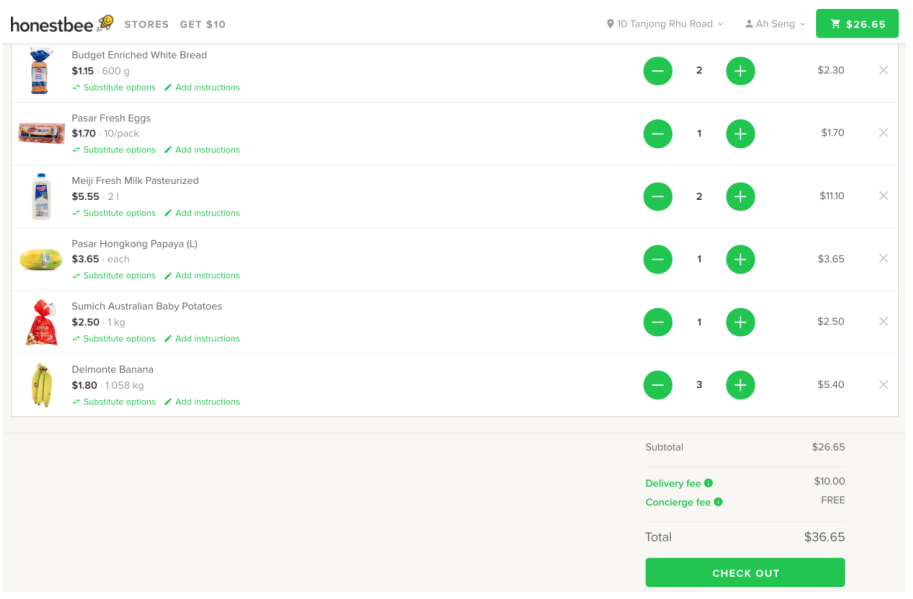
\includegraphics[width=0.6\paperwidth]{C:/Users/Admin/Desktop/Github/question_bank/LyX/static/img/9597-DHS-2016-P2-Q6-1}
\par\end{center}

In the event that the item is out of stock, the customer can also
opt for 3 options: 
\begin{center}
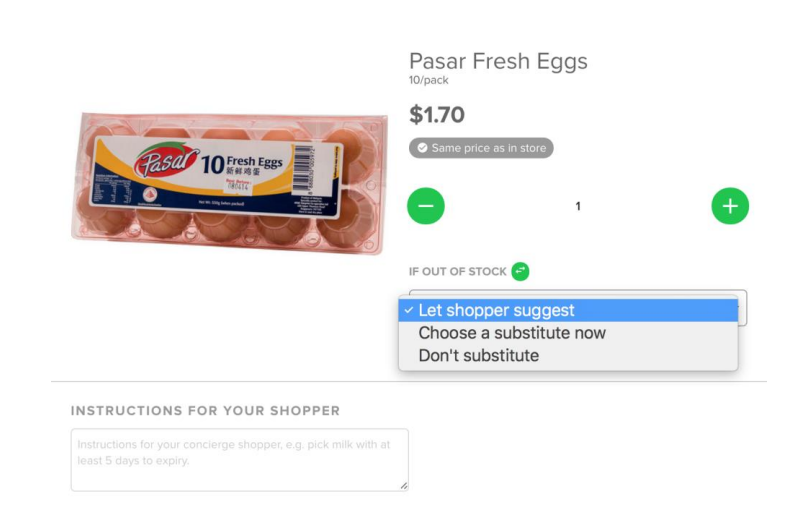
\includegraphics[width=0.6\paperwidth]{C:/Users/Admin/Desktop/Github/question_bank/LyX/static/img/9597-DHS-2016-P2-Q6-2}
\par\end{center}
\begin{enumerate}
\item Produce a normalised relational database schema showing the table
specifications. \hfill{}{[}8{]}
\item Draw an ER diagram illustrating the entities and their relationships.
\hfill{}{[}3{]}
\item Using suitable examples from this context, explain the concepts of
\begin{enumerate}
\item primary key (for the Customer table) \hfill{}{[}2{]}
\item composite key \hfill{}{[}2{]}
\item foreign key \hfill{}{[}2{]}
\end{enumerate}
\item Orders below \$30 is charged a delivery fee of \$10, else delivery
fee is waived. Some orders may incur a concierge fee for special instructions.
Where should fields such as delivery fee and concierge fee be stored?
Why? \hfill{}{[}2{]}
\end{enumerate}

 \newpage 

\item \textbf{{[}HCI/PRELIM/9597/2016/P1/Q1{]} }

A \textbf{\emph{palindrome}} is an integer that reads the same backwards
and forwards -- so 6, 11 and 121 are all palindromes, while 10, 12,
223 and 2244 are not (even though 010=10, we don't consider leading
zeroes when determining whether a number is a palindrome). 

A \textbf{\emph{fair and square}} number is an integer that is a \emph{palindrome}
\textbf{and} the \emph{square of a palindrome} at the same time. For
instance, 1, 9 and 121 are fair and square (being palindromes and
squares, respectively, of 1, 3 and 11), while 16, 22 and 676 are not
fair and square: 16 is \textbf{not} a palindrome, 22 is not a square,
and while 676 is a palindrome and a square number, it is the square
of 26, which is not a palindrome.

\subsection*{Task 1.1 }

Write program code with the following specification: 
\begin{itemize}
\item Input two integers -{}- the endpoints of an interval e.g. \texttt{100
1000 }
\item Output all fair and square numbers, if any, in the interval (inclusive
of endpoints). 
\item Output a count of the number of fair and square numbers in the interval.
\end{itemize}

\subsection*{Evidence 1: }

Your program code for Task 1.1.\hfill{} {[}8{]}

\subsection*{Evidence 2: }

Produce three screenshots showing the output of \texttt{1 4}, \texttt{10
120} and \texttt{100 1000} by the user.\hfill{} {[}3{]}

\subsection*{Task 1.2:}

Write program code to output the first 10 positive fair and square
numbers. 

\subsection*{Evidence 3: }

Your program code for Task 1.2.\hfill{} {[}3{]}

\subsection*{Evidence 4:}

Screenshot of output.\hfill{} {[}1{]}

 \newpage 

\item \textbf{{[}HCI/PRELIM/9597/2016/P1/Q2{]} }

The data file \texttt{FRUITS.txt} contains a list of fruit names. 

\subsection*{Task 2.1 }

Write program code to sort the fruit names in \texttt{FRUITS.txt}
in descending order using insertion sort. 

\subsection*{Evidence 5: }

Your program code for Task 2.1. \hfill{}{[}7{]}

\subsection*{Evidence 6: }

Screenshot of output. \hfill{}{[}1{]}

\subsection*{Task 2.2 }

Write program code to insert fruit names in \texttt{FRUITS.txt} to
a binary search tree using a linked structure.

\subsection*{Evidence 7:}

Your program code for Task 2.2. \hfill{}{[}8{]}

\subsection*{Task 2.3 }

Write program code to display the binary search tree contents in preorder,
inorder and postorder. 

\subsection*{Evidence 8: }

Your program code.\hfill{} {[}6{]}

\subsection*{Evidence 9: }

Screenshot of output.\hfill{} {[}3{]}

 \newpage 

\item \textbf{{[}HCI/PRELIM/9597/2016/P1/Q3{]} }

A transport company has a number of vehicles which can carry passengers.
Each vehicle is classified either as a bus or as a coach. All vehicles
have a registration number and have a certain number of seats for
the passengers. A bus can have a maximum number of standing passengers,
but a coach is not allowed to carry any standing passengers. Some
of the coaches are fitted with seat belts, but seat belts are never
fitted in a bus.

The transport company currently has a data file,\texttt{ VEHICLE.dat},
stores the following data:
\begin{itemize}
\item \texttt{RegNo} is used to uniquely identify a particular vehicle.
A typical vehicle registration number comes in the format \textquotedbl SBA1234\textquotedbl :
\begin{itemize}
\item S -- vehicle class (\textquotedbl S\textquotedbl{} stands for a
private vehicle) 
\item BA -- alphabetical series (\textquotedbl I\textquotedbl{} and \textquotedbl O\textquotedbl{}
are not used to avoid confusion with \textquotedbl 1\textquotedbl{}
and \textquotedbl 0\textquotedbl ) 
\item 1234 -- numerical series 
\end{itemize}
\item \texttt{NoOfSeats} is the maximum number of seats for passengers that
each vehicle can carry. 
\item \texttt{VehicleType} is the type of the vehicle and can take one of
the two values: \textquoteleft \texttt{B}\textquoteright{} for a bus
and \textquoteleft C\textquoteright{} for a coach. 
\end{itemize}
\texttt{VEHICLE.dat} has the following structure: 

\noindent %
\noindent\begin{minipage}[t]{1\columnwidth}%
\texttt{<NumberOfRecords>}

\texttt{<RegNo>|<NoOfSeats>|<VehicleType> }

\texttt{<RegNo>|<NoOfSeats>|<VehicleType> }

\texttt{. . . . . . . . . . . . . . . }

\texttt{. . . . . . . . . . . . . . . }

\texttt{<RegNo>|<NoOfSeats>|<VehicleType> }%
\end{minipage}

\texttt{NumberOfRecords} is the number of records in the file.

\subsection*{Task 3.1 }

Complete the test case table with the addition of \textbf{three} more
invalid vehicle registration numbers. The reasons for their invalidity
should be different.

The return value is a code as follows: 
\begin{itemize}
\item 0 -- valid registration number 
\item 1 -- the registration number was not 7 characters 
\item you will use other integer numbers for other invalid cases.

\begin{tabular}{|c|c|c|c|}
\hline 
Test Number & \texttt{RegNo} & Return value & Explanation of the test case\tabularnewline
\hline 
1 & \texttt{SBA1234} & \texttt{0} & Valid registration number\tabularnewline
\hline 
2 &  &  & \tabularnewline
\hline 
3 &  &  & \tabularnewline
\hline 
4 &  &  & \tabularnewline
\hline 
\end{tabular}
\end{itemize}

\subsection*{Evidence 10: }

The completed test case table. \hfill{}{[}3{]}

\subsection*{Task 3.2 }

Write program code for a function to validate a registration number.
The function header has the format:
\noindent \begin{center}
\texttt{FUNCTION ValidateRegNo(ThisRegNo : STRING) RETURNS INTEGER }
\par\end{center}

Write a program to:
\begin{itemize}
\item Input a registration number by the user 
\item Validate the input using the function \texttt{ValidateRegNo} 
\item Output a message describing the validity of the input.
\end{itemize}

\subsection*{Evidence 11:}
\begin{itemize}
\item Program code for the function \texttt{ValidateRegNo}\hfill{} {[}4{]}
\item Three screenshots showing the testing of Test Numbers 2, 3 and 4..
\hfill{}{[}3{]}
\end{itemize}
Additional data now needs to be stored about the vehicle:
\begin{itemize}
\item \texttt{MaxStanding} is the maximum number of standing passengers
that a vehicle classified as of type \textquoteleft \texttt{B}\textquoteright{}
can carry.
\item \texttt{SeatBeltsFitted} is a field that indicates whether a vehicle
of type \textquoteleft \texttt{C}\textquoteright{} has fitted with
seat belts.
\end{itemize}
The program design to process data about the vehicles is to be implemented
with objectoriented programming with the following three classes: 
\begin{center}
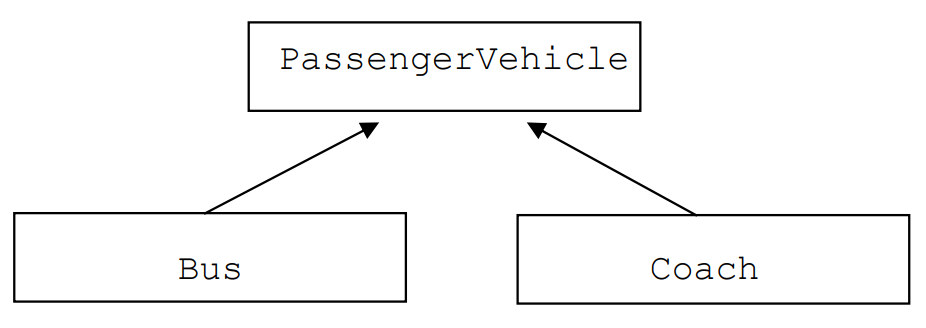
\includegraphics[width=0.35\paperwidth]{C:/Users/Admin/Desktop/Github/question_bank/LyX/static/img/9597-HCI-2016-P1-Q3-1}
\par\end{center}

\subsection*{Task 3.3 }

Write program code for the three classes shown. Evidence 12: Program
code for the three classes. \hfill{}{[}6{]}

\subsection*{Task 3.4 }

The data in \texttt{VEHICLE.dat} does not currently contain the following
additional data: 
\begin{itemize}
\item MaxStanding 
\item SeatBeltsFitted 
\end{itemize}
Write code to read a record from \texttt{VEHICLE.dat} and write the
updated record to \texttt{UVEHICLE.dat}.

As the data on each vehicle is read it should be displayed and the
user should be allowed to input the additional data required.

The user should be prompted to input the data item appropriate to
the type of vehicle.

The number of standing passengers is never more than 15.

For a \textquoteleft \texttt{C}\textquoteright{} type vehicle the
\texttt{MaxStanding} field should contain a zero value. 

The \texttt{SeatBeltsFitted} field should contain an appropriate value.
You are expected to make use of the classes you designed in Task 3.3.

\subsection*{Evidence 13: }

Program code for Task 3.4.\hfill{} {[}10{]}

\subsection*{Evidence 14: }

Screenshot showing the contents of \texttt{UVEHICLE.dat} from running
the program.\hfill{} {[}2{]}

 \newpage 

\item \textbf{{[}HCI/PRELIM/9597/2016/P1/Q4{]} }

A program is to be written to represent and implement a linked list
of nodes. Each node contains a string data value and a pointer. The
pointers link the data items in alphabetical order. 

The unused nodes are linked as shown below. The first unused node
is the position where the next new data item is to be stored. 
\begin{center}
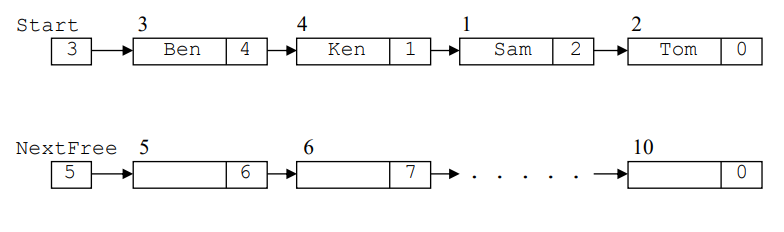
\includegraphics[width=0.65\paperwidth]{C:/Users/Admin/Desktop/Github/question_bank/LyX/static/img/9597-HCI-2016-P1-Q4-1}
\par\end{center}

The diagram shows the linked list with:
\begin{itemize}
\item the names \texttt{Sam}, \texttt{Tom}, \texttt{Ben} and \texttt{Ken}
(added in that order). 
\item the unused nodes linked together. 
\end{itemize}
The program will use a user-defined type \texttt{ListNode} for each
node defined as follows:
\noindent \begin{center}
\begin{tabular}{|c|c|c|}
\hline 
Identifier & Data Type & Description\tabularnewline
\hline 
\texttt{DataValue} & \texttt{STRING} & The node data\tabularnewline
\hline 
\texttt{PointerValue} & \texttt{INTEGER} & The node pointer \tabularnewline
\hline 
\end{tabular}
\par\end{center}

A linked list is implemented as an instance of the class \texttt{LinkedList}.
The class \texttt{LinkedList} has the following properties and methods:
\begin{center}
\begin{tabular}{|l|l|l|}
\hline 
\multicolumn{3}{|c|}{\texttt{Class: LinkedList}}\tabularnewline
\hline 
\multicolumn{3}{|c|}{Properties}\tabularnewline
\hline 
\texttt{\hspace{0.01\columnwidth}}Identifier & \texttt{\hspace{0.01\columnwidth}}Data Type & \texttt{\hspace{0.05\columnwidth}}Description\tabularnewline
\hline 
\texttt{Node} & \texttt{ARRAY{[}10{]} OF ListNode} & The linked list data structure -- data values and pointers. The array
index starts at 1. For testing purposes, the dataset has a maximum
of 10 items.\tabularnewline
\hline 
\texttt{Start} & \texttt{INTEGER} & Index position of the node at the start of the linked list. \tabularnewline
\hline 
\texttt{NextFree} & \texttt{INTEGER} & Index position of the next unused node.\tabularnewline
\hline 
\end{tabular}
\par\end{center}

\begin{center}
\begin{tabular}{|l|l|l|}
\hline 
\multicolumn{3}{|c|}{Methods}\tabularnewline
\hline 
\texttt{Initialise} & \texttt{PROCEDURE} & Sets all node data values to empty string. Set pointers to indicate
all nodes are unused and linked. Initialise values for \texttt{Start}
and \texttt{NextFree}.\tabularnewline
\hline 
\texttt{AddNode} & \texttt{PROCEDURE} & Add a new data item to the linked list. \tabularnewline
\hline 
\texttt{RemoveNode} & \texttt{PROCEDURE} & Remove a data item from the linked list.\tabularnewline
\hline 
\texttt{Display} & \texttt{PROCEDURE} & Display the current state of pointers and the array contents.\tabularnewline
\hline 
\texttt{IsEmpty} & \texttt{BOOLEAN FUNCTION} & Test for empty linked list. \tabularnewline
\hline 
\texttt{IsFull} & \texttt{BOOLEAN FUNCTION} & Test for no unused nodes.\tabularnewline
\hline 
\end{tabular}
\par\end{center}

\subsection*{Task 4.1 }

Write program code that repeatedly: 
\begin{itemize}
\item displays a menu with the following choices: 
\begin{enumerate}
\item[1.]  Add an item
\item[2.]  Remove an item 
\item[3.]  Output all pointers and data values 
\item[4.]  Exit 
\end{enumerate}
\item calls an appropriate procedure depending on the user\textquoteright s
choice. 
\end{itemize}

\subsection*{Evidence 15: }

Program code for Task 4.1. \hfill{}{[}5{]}

\subsection*{Task 4.2 }

Write program code for the classes \texttt{ListNode} and \texttt{LinkedList}.
Including the \texttt{Initialise}, \texttt{IsEmpty}, \texttt{IsFull}
and \texttt{Display} methods. The code should follow the specification
given. Do not attempt to write the methods \texttt{AddNode} and \texttt{RemoveNode}
at this stage.

\subsection*{Evidence 16: }

Program code for the \texttt{ListNode} and \texttt{LinkedList} classes
\hfill{}{[}10{]}

\subsection*{Task 4.3 }

Write code to create a \texttt{LinkedList} object in the main program. 

Run the program and select menu choice 3 to confirm the initial values
of the pointers and data values when the linked list is empty. 

\subsection*{Evidence 17:}

Screenshot confirming all values after initialisation of the \texttt{LinkedList}
object.\hfill{} {[}2{]}

Consider the \texttt{AddNode} method. The following pseudocode adds
a new data item to the linked list. The algorithm uses the variables
below:
\begin{center}
\begin{tabular}{|l|l|l|}
\hline 
\texttt{\hspace{0.01\columnwidth}}Identifier & \texttt{\hspace{0.01\columnwidth}}Data Type & \texttt{\hspace{0.05\columnwidth}}Description\tabularnewline
\hline 
NewItem & STRING & New data item input by the user\tabularnewline
\hline 
Found & BOOLEAN & lags to TRUE when the position at which to insert the new item has
been found\tabularnewline
\hline 
Current & INTEGER & array index position during list traversal\tabularnewline
\hline 
Previous & INTEGER & Previous array index position during list traversal\tabularnewline
\hline 
Temp & INTEGER & Temporary storage of pointer value\tabularnewline
\hline 
\end{tabular}
\par\end{center}

\noindent %
\noindent\begin{minipage}[t]{1\columnwidth}%
\texttt{PROCEDURE AddNode}

\texttt{\qquad{}INPUT NewItem}

\texttt{\qquad{}Node{[}NextFree{]}.DataValue = NewItem}

\texttt{\bigskip{}
}

\texttt{\qquad{}Temp = NextFree }

\texttt{\qquad{}NextFree = Node{[}NextFree{]}.PointerValue }

\texttt{\bigskip{}
}

\texttt{\qquad{}\# traverse the list to find the position to }

\texttt{\qquad{}\# insert the new item }

\texttt{\qquad{}Found = False }

\texttt{\qquad{}Current = Start }

\texttt{\qquad{}Previous = 0}

\texttt{\bigskip{}
}

\texttt{\qquad{}WHILE NOT Found AND Current != 0 }

\texttt{\qquad{}\qquad{}IF NewItem > Node{[}Current{]}.DataValue}

\texttt{\qquad{}\qquad{}\qquad{}THEN}

\texttt{\qquad{}\qquad{}\qquad{}\qquad{}\# move on to the next
node }

\texttt{\qquad{}\qquad{}\qquad{}\qquad{}Previous = Current }

\texttt{\qquad{}\qquad{}\qquad{}\qquad{}Current = Node{[}Current{]}.PointerValue}

\texttt{\qquad{}\qquad{}\qquad{}ELSE }

\texttt{\qquad{}\qquad{}\qquad{}\qquad{}Found = True }

\texttt{\qquad{}\qquad{}ENDIF}

\texttt{\qquad{}ENDWHILE}

\texttt{\bigskip{}
}

\texttt{\qquad{}IF Previous = 0 }

\texttt{\qquad{}\qquad{}THEN }

\texttt{\qquad{}\qquad{}\qquad{}\# new item will become the start
of the list}

\texttt{\qquad{}\qquad{}\qquad{}Start = Temp }

\texttt{\qquad{}\qquad{}\qquad{}Node{[}Temp{]}.PointerValue = Current }

\texttt{\qquad{}\qquad{}ELSE}

\texttt{\qquad{}\qquad{}\qquad{}\# new item is between previous
and current }

\texttt{\qquad{}\qquad{}Node{[}Previous{]}.PointerValue = Temp}

\texttt{\qquad{}\qquad{}Node{[}Temp{]}.PointerValue = Current }

\texttt{\qquad{}ENDIF }

\texttt{ENDPROCEDURE}%
\end{minipage}

Identifier Data Type Description F Current Note: The above pseudocode
is available in the text file \texttt{PSEUDOCODE\_TASK\_4\_4.txt}

\subsection*{Task 4.4 }

Write code to implement the \texttt{AddNode} method for the \texttt{LinkedList}
class. 

You may use the text file \texttt{PSEUDOCODE\_TASK\_4\_4.txt} as a
basis for the writing of your code.

The main program should check each time that the \texttt{LinkedList}
object is not full before using the \texttt{AddNode} method.

Run the program as follows: 
\begin{itemize}
\item Menu choice 1 four times, inputting the data values:

\texttt{Sam}, \texttt{Tom}, \texttt{Ben}, \texttt{Ken} in that order. 
\item Menu choice 3 to display.
\end{itemize}

\subsection*{Evidence 18: }

Your program code for Task 4.4. \hfill{}{[}5{]}

\subsection*{Evidence 19: }

Screenshot showing the pointers and the addition of the four nodes
to the linked list. \hfill{}{[}2{]}

\subsection*{Task 4.5 }

Write code to implement the \texttt{RemoveNode} method for the \texttt{LinkedList}
class. 

The main program should check each time that the LinkedList object
is not empty before using the \texttt{RemoveNode} method. Node removed
from the linked list should be returned to the NextFree list. 

Run the program as follows: 
\begin{itemize}
\item Menu choice 1 four times, inputting the data values: 

\texttt{Sam}, \texttt{Tom}, \texttt{Ben}, \texttt{Ken} in that order. 
\item Menu choice 2 two times, inputting the data values: 

\texttt{Sam}, \texttt{Ben} in that order.
\item Menu choice 3 to display. 
\end{itemize}

\subsection*{Evidence 20: }

Your program code for Task 4.5. \hfill{}{[}6{]}

\subsection*{Evidence 21: }

Screenshot showing the pointers and data values after the addition
of the four nodes followed by the removal of two nodes to the linked
list. \hfill{}{[}2{]}

 \newpage 

\item \textbf{{[}HCI/PRELIM/9597/2016/P2/Q1{]} }

Using the information in the table below, assuming that the project
team will work a standard working week (5 working days in 1 week)
and that all tasks will start as soon as possible: 
\noindent \begin{center}
\begin{tabular}{|c|l|c|c|}
\hline 
Task & Description & Duration (Working Days) & Predecessor/s \tabularnewline
\hline 
A & Requirement Analysis & 5 & -\tabularnewline
\hline 
B & Systems Design & 15 & A\tabularnewline
\hline 
C & Programming & 25 & B\tabularnewline
\hline 
D & Telecoms & 15 & B\tabularnewline
\hline 
E & Hardware Installation & 30 & B\tabularnewline
\hline 
F & Integration & 10 & C, D\tabularnewline
\hline 
G & System Testing & 10 & E, F\tabularnewline
\hline 
H & Training/Support & 5 & G\tabularnewline
\hline 
I & Handover and Go-Liv & 5 & H\tabularnewline
\hline 
\end{tabular}
\par\end{center}
\begin{enumerate}
\item Draw a Program Evaluation and Review Technique (PERT) chart, show
clearly the early start and late start time of each task, showing
dummy tasks, where necessary. \hfill{}{[}4{]}
\item Explain the nature and purpose of a dummy activity. \hfill{}{[}2{]}
\item Explain dependent stages and concurrent stages, giving examples from
your chart. \hfill{}{[}2{]}
\item State the critical path and the minimum time in which the project
can be completed in weeks.\hfill{} {[}2{]}
\item Identify any non-critical tasks and the float (free slack) on each.\hfill{}
{[}2{]}
\item Produce a Gantt chart based on the above information.\hfill{} {[}2{]}
\end{enumerate}

 \newpage 

\item \textbf{{[}HCI/PRELIM/9597/2016/P2/Q2{]} }

The owner of HC Book Caf� wishes to converts his book caf� into a
self-service book club caf� for members only. All access to food or
books is via a \textquotedblleft vending machine\textquotedblright{}
concept using the member\textquoteright s card. 

There is a stock of 2000 different book titles and multiple copies
of popular titles. Books may be hired by members. Different rates
are charged for different books. Members are allowed to hire no more
than 5 items at anytime. 

Members can enjoy a light snack while viewing their favourite book.
If the book is returned the same day via the book drop, hire charges
are not incurred. All food and hire charges incurred for the month
is billed to the member every 12th of the following month. Cash transaction
is not available. 

The shop owner wishes to computerize the system to handle the various
transactions and stock control. The system should also perform the
following functions: 
\begin{itemize}
\item Hold up-to-date details of members and stock
\item Allow enquiry to determine the whereabouts, and dates of return, of
particular books 
\item Produce an itemized bill for each customer at end of each month.
\end{itemize}
\begin{enumerate}
\item The system analyst of a software house was to design the computerized
system. What documentation should the system analyst produce and state
5 necessary contents of the documentation? Who would use it and state
2 reasons for use.\hfill{} {[}8{]}
\item List the files, giving details of the fields which it may contain,
that would be required for this system, and draw the data flow diagram
of the computerized system. \hfill{} {[}12{]}
\item HC Book Caf� offers a member loyalty program that offers a range of
discounts. For members in the loyalty program between 3 to 5 years,
they will receive a 5\% discount. For more than 5 years, the member
will receive a 10\% discount. However, whether a member is in the
loyalty program or not, if the cumulative value of his transactions
for this calendar year exceed \$1000, he will receive a 15\% discount.
However, note that aggregation of discounts is not allowed. 
\begin{enumerate}
\item Create a decision table that shows all possible outcomes for the above
loyalty program. 
\item Draw the decision table after redundancies have been removed. \hfill{}
{[}5{]}
\end{enumerate}
\end{enumerate}

 \newpage 

\item \textbf{{[}HCI/PRELIM/9597/2016/P2/Q3{]} }

Given two positive integers \texttt{M} and \texttt{N}, the function
\texttt{GCD(M, N)} is defined by 
\begin{enumerate}
\item[(i)]  If \texttt{M < N}, swap \texttt{M} and \texttt{N} 
\item[(ii)]  Divide \texttt{M} by \texttt{N} and let \texttt{R} be the remainder.
If \texttt{R = 0}, \texttt{N} is the answer 
\item[(iii)]  Set \texttt{M = N}, \texttt{N = R} and go back to step (i)
\end{enumerate}
Produce a recursive solution for \texttt{GCD(M,N)} using pseudocode.
You may assume the availability of the operator \texttt{MOD} as in
part \textbf{(b)}.\hfill{} {[}6{]}

 \newpage 

\item \textbf{{[}HCI/PRELIM/9597/2016/P2/Q4{]} }
\begin{enumerate}
\item Explain what is meant by ASCII code and Unicode.\hfill{} {[}4{]}
\item A number is stored as a one byte binary integer. How would the number
99 be represented as a one byte binary? \hfill{}{[}2{]}
\item Convert the number 99 into hexadecimal. \hfill{}{[}2{]}
\item Give two reasons why hexadecimal numbers are used in computing. \hfill{}{[}2{]}
\end{enumerate}

 \newpage 

\item \textbf{{[}HCI/PRELIM/9597/2016/P2/Q5{]} }
\begin{enumerate}
\item Using the 3 design principle you have learnt in class to assess the
interfaces between IOS and Android for mobile. Redraw and complete
the table with your points. You may draw user interfaces to illustrate
your point. \hfill{}{[}15{]}
\noindent \begin{center}
\begin{tabular}{|l|c|c|}
\hline 
Design Principals & IOS & Android\tabularnewline
\hline 
Principal 1 &  & \tabularnewline
\hline 
Principal 2 &  & \tabularnewline
\hline 
Principal 3  &  & \tabularnewline
\hline 
\end{tabular}
\par\end{center}
\item From the table above, draw a brief conclusion on the usability of
the above platforms.\hfill{} {[}3{]}
\end{enumerate}

 \newpage 

\item \textbf{{[}HCI/PRELIM/9597/2016/P2/Q6{]} }

A relational database is to be used by the Human Resource department
to recruit and register new students at the beginning of each year.
Four tables present in the database are STUDENT, SCHOOL, GRADES, REGISTRATION. 

A brief description of the tables are as follow: 
\begin{itemize}
\item STUDENT table stores the demographic information of students
\item SCHOOL table stores information of the school they are currently studying
\item GRADES table stores information of the subjects and grades of the
student in the previous year
\item REGISTRATION ties together all the relevant information of the students
from other tables and their registration details
\end{itemize}
\begin{enumerate}
\item Draw an E-R diagram to show the relationship between the four tables
that provides for a fully normalized database design. \hfill{} {[}6{]}

A table description can be expressed as: 

\texttt{Tablename{[}Attribute1, Attribute2, \dots .. {]} }

The primary key is indicated by underlining one or more attributes. 
\end{enumerate}
(b) Give a table description for all the tables. Ensure there are
at least 2 attributes in addition to the primary key.\hfill{} {[}12{]}

 \newpage 

\item \textbf{{[}HCI/PRELIM/9597/2016/P2/Q7{]} }

Cloud computing is widely used in education to facilitate teaching
and learning in classrooms. 
\begin{enumerate}
\item How is computing from the Cloud different from computing traditionally?
\hfill{}{[}2{]}
\item What are the benefits of cloud computing?\hfill{} {[}4{]}
\item How can Cloud computing assist you as a student in project management?
\hfill{}{[}3{]}
\end{enumerate}

 \newpage 

\item \textbf{{[}PJC/PRELIM/9597/2016/P1/Q1{]} }

Four stories are given in four data files: \texttt{AIRCON.txt}, \texttt{BLIND.txt},
\texttt{COMP.txt}, \texttt{EMPEROR.txt}. The task is to find the frequency
of alphabets used in the stories. 

\subsection*{Task 1.1 }

Count the alphabets in each story and display the frequency of each
alphabet in a table form. Do not distinguish between upper and lower
cases. Do not count non-alphabets. Frequency should be displayed in
descending order. Display alphabets with same frequency in ascending
order. 

Sample output: 
\noindent \begin{center}
\begin{tabular}{lll}
\texttt{Alphabet} & \texttt{Frequency} & \tabularnewline
\texttt{e} & \texttt{20} & \tabularnewline
\texttt{t} & \texttt{14} & \tabularnewline
\cline{3-3} 
\texttt{a} & \multicolumn{1}{l|}{\texttt{12}} & \multicolumn{1}{l|}{\texttt{a} and \texttt{i} have same frequency of 12,}\tabularnewline
\texttt{i} & \multicolumn{1}{l|}{\texttt{12}} & \multicolumn{1}{l|}{display \texttt{a} before \texttt{i}, since \texttt{a} comes before
\texttt{i}}\tabularnewline
\cline{3-3} 
\texttt{o} & \texttt{10} & \tabularnewline
\texttt{u} & \texttt{6} & \tabularnewline
\cline{3-3} 
\texttt{g} & \multicolumn{1}{l|}{\texttt{3}} & \multicolumn{1}{l|}{\texttt{g} and \texttt{j} have same frequency of 12,}\tabularnewline
\texttt{j} & \multicolumn{1}{l|}{\texttt{3}} & \multicolumn{1}{l|}{display \texttt{g} before \texttt{j,} since \texttt{g} comes before
\texttt{j}}\tabularnewline
\cline{3-3} 
\texttt{z} & \texttt{1} & \tabularnewline
\end{tabular}
\par\end{center}

\subsection*{Evidence 1: }

Your program code for task 1.1.\hfill{} {[}9{]}

\subsection*{Evidence 2: }

Screenshot of running \texttt{AIRCON.txt} data file.\hfill{} {[}1{]}

\subsection*{Task 1.2 }

Amend your program code to display alphabets and frequencies in all
four files in a table form, with alphabets in first column and frequencies
of alphabets in subsequent columns. Display in alphabetical order
as shown in following sample output: 
\noindent \begin{center}
\begin{tabular}{|l|l|l|l|l|}
\hline 
\texttt{Alphabet} & \texttt{AIRCON.txt} & \texttt{BLIND.txt} & \texttt{COMP.txt} & \texttt{EMPEROR.txt}\tabularnewline
\hline 
\texttt{a} & \texttt{115} & \texttt{471} & \texttt{604} & \texttt{490}\tabularnewline
\hline 
\texttt{b} & \texttt{25} & \texttt{87} & \texttt{111} & \texttt{56}\tabularnewline
\hline 
\texttt{c} & \texttt{46} & \texttt{117} & \texttt{230} & \texttt{107}\tabularnewline
\hline 
\texttt{$\vdots$} & \texttt{$\vdots$} & \texttt{$\vdots$} & \texttt{$\vdots$} & \texttt{$\vdots$}\tabularnewline
\hline 
\texttt{$\vdots$} & \texttt{$\vdots$} & \texttt{$\vdots$} & \texttt{$\vdots$} & \texttt{$\vdots$}\tabularnewline
\hline 
\texttt{x} & \texttt{3} & \texttt{6} & \texttt{9} & \texttt{0}\tabularnewline
\hline 
\texttt{y} & \texttt{38} & \texttt{121} & \texttt{128} & \texttt{130}\tabularnewline
\hline 
\texttt{z} & \texttt{2} & \texttt{3} & \texttt{4} & \texttt{4}\tabularnewline
\hline 
\end{tabular}
\par\end{center}

\subsection*{Evidence 3: }

Your amended program code for task 1.2. \hfill{}{[}8{]}

\subsection*{Evidence 4: }

Screenshot of running your program code.\hfill{} {[}1{]}

 \newpage 

\item \textbf{{[}PJC/PRELIM/9597/2016/P1/Q2{]} }

Write a program to encrypt and decrypt user passwords. 

\subsection*{Task 2.1}

A set of encryption key is given in the data file \texttt{ENCRYPT\_KEY.txt}.
The encryption key will map each alphabet and number according to
the table below.
\noindent \begin{center}
\texttt{}%
\begin{tabular}{ccc}
\texttt{a \textrightarrow{} m} & \texttt{m \textrightarrow{} q} & \texttt{y \textrightarrow{} c}\tabularnewline
\texttt{b \textrightarrow{} h} & \texttt{n \textrightarrow{} s} & \texttt{z \textrightarrow{} a}\tabularnewline
\texttt{c \textrightarrow{} t} & \texttt{o \textrightarrow{} l} & \texttt{0 \textrightarrow{} 7}\tabularnewline
\texttt{d \textrightarrow{} f} & \texttt{p \textrightarrow{} n} & \texttt{1 \textrightarrow{} 3}\tabularnewline
\texttt{e \textrightarrow{} g} & \texttt{q \textrightarrow{} i} & \texttt{2 \textrightarrow{} 8}\tabularnewline
\texttt{f \textrightarrow{} k} & \texttt{r \textrightarrow{} u} & \texttt{3 \textrightarrow{} 9}\tabularnewline
\texttt{g \textrightarrow{} b} & \texttt{s \textrightarrow{} o} & \texttt{4 \textrightarrow{} 5}\tabularnewline
\texttt{h \textrightarrow{} p} & \texttt{t \textrightarrow{} x} & \texttt{5 \textrightarrow{} 6}\tabularnewline
\texttt{i \textrightarrow{} j} & \texttt{u \textrightarrow{} z} & \texttt{6 \textrightarrow{} 0}\tabularnewline
\texttt{j \textrightarrow{} w} & \texttt{v \textrightarrow{} y} & \texttt{7 \textrightarrow{} 1}\tabularnewline
\texttt{k \textrightarrow{} e} & \texttt{w \textrightarrow{} v} & \texttt{8 \textrightarrow{} 4}\tabularnewline
\texttt{l \textrightarrow{} r} & \texttt{x \textrightarrow{} d} & \texttt{9 \textrightarrow{} 2}\tabularnewline
\end{tabular}
\par\end{center}

For example, \texttt{a} is mapped to \texttt{m}, \texttt{b} mapped
to \texttt{h}, m mapped to \texttt{q}, \texttt{9} mapped to \texttt{2},
etc. The mapping is case-sensitive for alphabets. Therefore a password
\texttt{WhizKid123} will be encrypted to \texttt{VpjaEjf389}.

Conversely, decryption works in the opposite way. Hence the password
\texttt{VpjaEjf389} will be decrypted to \texttt{WhizKid123}. 

There is no mapping for symbols. Some examples of symbols are \texttt{!},\texttt{
@}, \texttt{\#}, \texttt{\$}, \texttt{\%}, \texttt{\textasciicircum}.
Hence, a password \texttt{Extr@123} will be encrypted to \texttt{Gdxu@389},
where the symbol remains the same. 

\textbf{\emph{Copy and paste}} the encryption key (from data file
\texttt{ENCRYPT\_KEY.txt})\textbf{\emph{ into your program code}}
and \textbf{\emph{make use of it}} to write a program that 
\begin{itemize}
\item Allows a user to select option to \textbf{\emph{encrypt}} or \textbf{\emph{decrypt}}
a user password
\item Gets user input of the password,
\item Encrypts (or decrypts) the password according to user\textquoteright s
option, 
\item Displays the encrypted or decrypted password 
\end{itemize}

\subsection*{Evidence 5: }

Your program code for task 2.1.\hfill{} {[}8{]}

\subsection*{Evidence 6:}

Screenshot of running program by encrypting \texttt{WhizKid123} and
decrypting \texttt{XgteV\textasciicircum cg84}.\hfill{} {[}1{]}

\subsection*{Task 2.2 }

Amend your program code into a function that accepts two parameters
-- \textquotedbl\texttt{password}\textquotedbl{} and \textquotedbl\texttt{encrypt}\textquotedbl ,
and returns the encrypted or decrypted password. 

\texttt{FUNCTION Cryptograph(password:STRING, encrypt:BOOLEAN):RETURN
STRING }

\subsection*{Evidence 7: }

Your program code for task 2.2.\hfill{} {[}4{]}

\subsection*{Task 2.3 }

Write program code that makes use of the function \texttt{Cryptograph}
from task 2.2 that reads all the passwords in data file \texttt{PASSWORDS.txt},
encrypts and writes them into another file \texttt{CONVERTED.txt}. 

\begin{tabular}{l|l|l}
\cline{2-2} 
Sample input file:  & \texttt{WhizKid123 } & \tabularnewline
 & \texttt{Extr@123} & \tabularnewline
\cline{2-2} 
\multicolumn{1}{l}{} & \multicolumn{1}{l}{~~~~~~~~~~~$\downarrow$} & Encrypt and write\tabularnewline
\cline{2-2} 
Sample output file: & \texttt{VpjaEjf389} & \tabularnewline
 & \texttt{Gdxu@389} & \tabularnewline
\cline{2-2} 
\end{tabular}

\subsection*{Evidence 8: }

Program code for task 2.3. \hfill{}{[}3{]}

\subsection*{Evidence 9: }

Screenshot of output file \texttt{CONVERTED.txt}. \hfill{}{[}1{]}

 \newpage 

\item \textbf{{[}PJC/PRELIM/9597/2016/P1/Q3{]} }

Tic-tac-toe is a game in which two players take turns marking X and
O in the spaces in a $3\times3$ grid. The player who succeeds in
placing three of their marks in a horizontal, vertical, or diagonal
row wins the game.

For example, player who marks \texttt{X} wins this game. 
\noindent \begin{center}
\begin{tabular}{|c|c|c|}
\hline 
\texttt{X} & \texttt{O} & \tabularnewline
\hline 
\texttt{X} & \texttt{X} & \texttt{X}\tabularnewline
\hline 
\texttt{O} &  & \texttt{O}\tabularnewline
\hline 
\end{tabular}
\par\end{center}

The task is to write program code for a tic-tac-toe game for two human
players. 

\subsection*{Task 3.1 }

Decide on the design to be used for:
\begin{itemize}
\item the data structure to represent the $3\times3$ grid, using the identifier
\texttt{board}
\item the contents of the marks (\texttt{X}, \texttt{O} and blank) in the
spaces
\item how user input (\texttt{X} or \texttt{O}) in the spaces 
\end{itemize}

\subsection*{Evidence 10:}

Your program design. Include program code for board. \hfill{} {[}4{]}

\subsection*{Task 3.2 }

Write a function \texttt{displayBoard} that will display the game
\texttt{board} clearly to the players. You should use the board as
a parameter in \texttt{displayBoard}. 

Write another function \texttt{displayInstructions} to inform players
on how to input \texttt{X} and \texttt{O} in the spaces on the game
board. 

\subsection*{Evidence 11: }

Your functions \texttt{displayBoard} and \texttt{displayInstructions}.
\hfill{}{[}4{]}

\subsection*{Task 3.3 }

Write a function \texttt{getPlayerMove} to get players to make their
move (by marking \texttt{X} or \texttt{O}) on the board. You should
include validation on user input and check that the space is not already
occupied. Use \texttt{board} as a parameter. You may include any other
suitable parameters. 

\subsubsection*{Evidence 12: }

Your function \texttt{getPlayerMove}. \hfill{}{[}5{]}

\subsection*{Task 3.4 }

Write a function \texttt{checkWin} that checks all the conditions
for winning a game and returns \texttt{True} if a player has won the
game, otherwise return \texttt{False}. Use \texttt{board} as a parameter.
You may include any other suitable parameters. 

\subsection*{Evidence 13:}

Your function \texttt{checkWin}. \hfill{}{[}5{]}

\subsection*{Task 3.5}

Write a \texttt{main} function that makes use of the identifiers and
functions from task 3.1 to task 3.4 and allows two human players to
play a game of tic-tac-toe.

The \texttt{main} function should include the following: 
\begin{itemize}
\item give instructions to players on how to input \texttt{X} or \texttt{O} 
\item ask whether player 1 or player 2 starts first move 
\item ensure players 1 and 2 take turns to make their move 
\item display the game board after every move made by a player
\item check for winner
\item display message on which player has won the game or whether the game
ends in a draw
\end{itemize}

\subsection*{Evidence 14: }

Your \texttt{main} function. \hfill{} {[}8{]}

\subsection*{Evidence 15: }

Run your \texttt{main} function and produce screenshots of \textbf{three}
games where player 1 wins one game, player 2 wins another game, and
a drawn game. \hfill{}{[}3{]}

 \newpage 

\item \textbf{{[}PJC/PRELIM/9597/2016/P1/Q4{]} }

A college uses a binary tree structure to store its subjects offered
to students. 

The program will use a user-defined type \texttt{Node} for each node
defined as follows: 
\begin{center}
\begin{tabular}{|l|l|l|}
\hline 
\texttt{\hspace{0.01\columnwidth}}Identifier & \texttt{\hspace{0.01\columnwidth}}Data Type & \texttt{\hspace{0.05\columnwidth}}Description\tabularnewline
\hline 
\texttt{Subject} & \texttt{STRING} & The node's value for subject offered\tabularnewline
\hline 
\texttt{LeftPtr} & \texttt{INTEGER} & The left pointer for the node\tabularnewline
\hline 
\texttt{RightPtr} & \texttt{INTEGER} & The right pointer for the node\tabularnewline
\hline 
\end{tabular}
\par\end{center}

A linked list is maintained of all unused nodes which do not form
part of the tree. The first available node which is used for a new
item is indicated by NextFreePosition. Items in the unused list are
linked using their left pointers. 

The binary tree and linked list are implemented using variables as
follows: 
\begin{center}
\begin{tabular}{|l|l|l|}
\hline 
\texttt{\hspace{0.01\columnwidth}}Identifier & \texttt{\hspace{0.01\columnwidth}}Data Type & \texttt{\hspace{0.05\columnwidth}}Description\tabularnewline
\hline 
\texttt{SubjectTree} & \texttt{STRING} & The tree data\tabularnewline
\hline 
\texttt{Root} & \texttt{INTEGER} & Index position of the root node\tabularnewline
\hline 
\texttt{NextFreePosition} & \texttt{INTEGER} & Index for the next unused node\tabularnewline
\hline 
\end{tabular}
\par\end{center}

The diagram shows the binary tree and linked list after five subjects
have been added.
\begin{center}
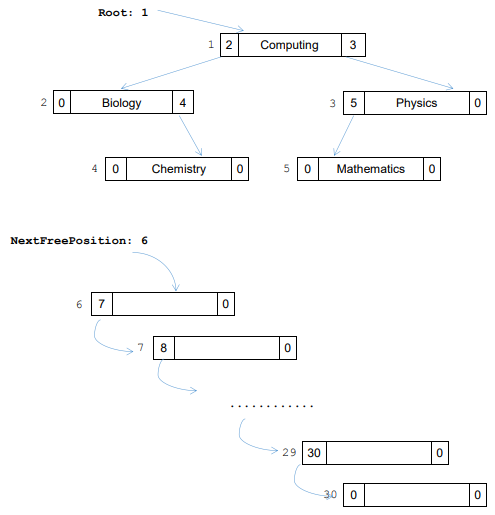
\includegraphics[width=0.5\paperwidth]{C:/Users/Admin/Desktop/Github/question_bank/LyX/static/img/9597-PJC-2016-P1-Q4-1}
\par\end{center}

\subsection*{Task 4.1 }

Write the program code to declare all the required variables and create
the initial linked list which contains all 30 nodes. 

Add statement(s) to initialise the empty tree. 

\subsection*{Evidence 16: }

Your program code for task 4.1. \hfill{}{[}8{]}

The following incomplete pseudocode inserts a data value into the
binary tree structure.

\noindent %
\noindent\begin{minipage}[t]{1\columnwidth}%
\texttt{PROCEDURE InsertBinaryTree(NewItem)}

\texttt{\qquad{}... ... }

\texttt{\qquad{}IF tree is empty }

\texttt{\qquad{}\qquad{}THEN }

\texttt{\qquad{}\qquad{}\qquad{}... ...}

\texttt{\qquad{}ELSE}

\texttt{\qquad{}\qquad{}//traverse the tree to find the insert position }

\texttt{\qquad{}\qquad{}... ... }

\texttt{\qquad{}\qquad{}LastMove = 'X'}

\texttt{\qquad{}\qquad{}REPEAT}

\texttt{\qquad{}\qquad{}\qquad{}PreviousPtr <- CurrentPtr }

\texttt{\qquad{}\qquad{}\qquad{}IF NewItem < CurrentPtr item}

\texttt{\qquad{}\qquad{}\qquad{}\qquad{}THEN }

\texttt{\qquad{}\qquad{}\qquad{}\qquad{}\qquad{}//move left}

\texttt{\qquad{}\qquad{}\qquad{}\qquad{}\qquad{}CurrentPtr <-
CurrentPtr's left pointer}

\texttt{\qquad{}\qquad{}\qquad{}\qquad{}\qquad{}LastMove = 'Left' }

\texttt{\qquad{}\qquad{}\qquad{}\qquad{}ELSE}

\texttt{\qquad{}\qquad{}\qquad{}\qquad{}\qquad{}//move right }

\texttt{\qquad{}\qquad{}\qquad{}\qquad{}\qquad{}CurrentPtr <-
CurrentPtr's right pointer }

\texttt{\qquad{}\qquad{}\qquad{}\qquad{}\qquad{}LastMove = 'Right'}

\texttt{\qquad{}\qquad{}\qquad{}ENDIF }

\texttt{\qquad{}\qquad{}UNTIL CurrentPtr = NULL }

\texttt{\qquad{}ENDIF }

\texttt{\qquad{}IF LastMove = 'Left'}

\texttt{\qquad{}... ... }

\texttt{\qquad{}ELSE IF LastMove = 'Right'}

\texttt{\qquad{}... ...}

\texttt{\qquad{}ENDIF }

\texttt{\qquad{}... ... }

\texttt{END PROCEDURE }%
\end{minipage}

\subsection*{Task 4.2 }

Complete the pseudocode and write a module \texttt{AddSubject} to
add a subject into the binary tree. 

\subsection*{Evidence 17:}

Your \texttt{AddSubject} program code. \hfill{} {[}7{]}

\subsection*{Task 4.3 }

Write a module \texttt{Display} to display the value of \texttt{Root},
the value of \texttt{NextFreePosition} and the contents of \texttt{SubjectTree}
in index order. 

\subsection*{Evidence 18: }

Your \texttt{Display} program code. \hfill{} {[}4{]}

\subsection*{Task 4.4}

Write a module \texttt{BuildTree} to construct a binary tree using
the data provided in the data file \texttt{SUBJECT.TXT}. Read in all
the data from the data file and use the \texttt{AddSubject} module. 

\subsection*{Evidence 19: }

Your \texttt{BuildTree} program code. \hfill{}{[}2{]}

\subsection*{Evidence 20:}

Run your program and produce screenshot of contents of binary tree.
\hfill{} {[}1{]}

Deleting a node from a tree may change the structure of the tree.
To simplify the deletion process, label a node as \textquotedblleft \texttt{deleted}\textquotedblright{}
but \textbf{do not remove the node} from the tree structure. After
that, regenerate the entire tree structure.

\subsection*{Task 4.5 }

Write a module \texttt{LabelDelete} that labels a node as \textquotedblleft \texttt{deleted}\textquotedblright{}
but do not remove the node from the tree structure. 

\subsection*{Evidence 21: }

Your LabelDelete program code. \hfill{}{[}6{]}

\subsection*{Task 4.6}

Write program code to regenerate the entire binary tree.

\subsection*{Evidence 22: }

Your program code to regenerate the binary tree. \hfill{}{[}6{]}

\subsection*{Evidence 23:}

Display a screenshot of the regenerated binary tree after deleting
\textquotedblleft \texttt{Chemistry}\textquotedblright{} and \textquotedblleft \texttt{History}\textquotedblright .
\hfill{} {[}1{]}

 \newpage 

\item \textbf{{[}PJC/PRELIM/9597/2016/P2/Q1{]} }

The PJC clinic has several doctors. When a patient wants to book an
appointment with a doctor, the patient rings the doctors' receptionist.
The receptionist asks for the following details:
\begin{itemize}
\item patient name 
\item first line of address
\item doctor requested 
\end{itemize}
The receptionist checks the files to ensure that the patient is registered
with the clinic. The receptionist looks to find the requested doctor's
free appointments in the appointments book. The receptionist offers
the patient a day and a time for the appointment. If this is agreed
then the patient's name is written in the space in the appointment
book for that day and time. 

At the beginning of every day, the receptionist types an appointment
list for each of the doctors for that day. The list contains the appointment
times and patients\textquoteright{} names. When the patient arrives
at the doctors' clinic for their appointment, they give their name
to the receptionist. The receptionist informs each doctor as their
patients arrive. 

The clinic has decided to replace this manual system with an on-line
computerised system. 

A \textbf{system developer} is employed to carry out the task. The
first task assigned to the system developer is to write a project
proposal. 
\begin{enumerate}
\item One section of the project proposal is the Problem Statement which
lists the problems in the current system. Write the \textbf{Problem
Statement}. {[}4{]}
\item The system developer has drawn up an initial plan of the work involved: 
\noindent \begin{center}
\begin{tabular}{|c|l|c|}
\hline 
\textbf{Stage} & \textbf{Activity} & \textbf{Weeks}\tabularnewline
\hline 
A & identify requirements & 3\tabularnewline
\hline 
B & produce design & 5\tabularnewline
\hline 
C & write code & 9\tabularnewline
\hline 
D & black box testing & 2\tabularnewline
\hline 
E & acceptance testing & 3\tabularnewline
\hline 
F & prepare documentation & 6\tabularnewline
\hline 
\end{tabular}
\par\end{center}

From this data, a Program Evaluation Review Technique (PERT) chart
is constructed. The stage is between the nodes in circles. 
\begin{center}
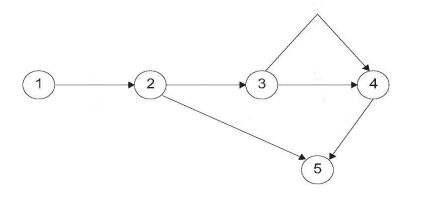
\includegraphics[width=0.5\paperwidth]{C:/Users/Admin/Desktop/Github/question_bank/LyX/static/img/9597-PJC-2016-P2-Q1-1}
\par\end{center}
\begin{enumerate}
\item Complete the PERT chart by writing the stage (A, B, \dots ) and duration
between the nodes. \hfill{}{[}4{]}
\item State the critical path. \hfill{}{[}1{]}
\item State the minimum time in which the project could be completed. \hfill{}{[}1{]}
\item For activity D: 
\begin{enumerate}
\item[(iv.1)]  state the earliest start time. \hfill{}{[}1{]}
\item[(iv.2)]  state the latest finish time. \hfill{}{[}1{]}
\end{enumerate}
\item Two stages start and end at the same nodes. Re-draw the PERT chart
by using an extra dummy stage separating them. Explain the nature
and purpose of a dummy stage. \hfill{}{[}2{]}
\item Explain dependent stages and concurrent stages. For each type of stage
give an example from this chart. \hfill{}{[}4{]}
\item Draw a Gantt chart showing all stages and their dependencies.\hfill{}
{[}4{]}
\end{enumerate}
\item Describe any \textbf{three} key stages (System analysis, System design,
System development, Testing, Implementation of computer system, Documentation,
Maintenance) of the software development life cycle. \hfill{}{[}6{]}
\item Explain why the problem must be defined accurately before the analyst
starts work. \hfill{}{[}2{]}
\item Name two methods the analyst could use to gather information about
the existing manual system. Explain how each method would be used
to gather information about this manual system. \hfill{}{[}4{]}
\item When the receptionist types an appointment for a patient, explain
why the patient name and first line of address need to be entered.
\hfill{}{[}2{]}
\item The following pseudocode algorithm describes one method of finding
an arbitrary patient name in an alphabetically ordered array of \texttt{N}
unique names. 

\noindent\begin{minipage}[t]{1\columnwidth}%
\texttt{SET first to 1 }

\texttt{SET last to N }

\texttt{REPEAT }

\texttt{\qquad{}SET mid to the integer part of (first + last)/2 }

\texttt{\qquad{}IF the mid name precedes the wanted name }

\texttt{\qquad{}\qquad{}THEN SET first to mid + 1 }

\texttt{\qquad{}ELSE }

\texttt{\qquad{}\qquad{}SET last to mid \textendash{} 1 }

\texttt{\qquad{}ENDIF }

\texttt{UNTIL first > last OR mid name is the wanted name }%
\end{minipage}
\begin{enumerate}
\item If 142 patients\textquoteright{} names are stored in the array, and
Natasha is the 44th name, state the elements of the array that are
examined when searching for Natasha.\hfill{} {[}2{]}
\item If a search is made for a name that is not in the array, what is the
largest number of elements that might need to be examined before one
could say that the name is not present? Explain how you arrive at
your answer. \hfill{}{[}2{]}
\end{enumerate}
\item Before releasing the software, it is tested using a variety of strategies.
Describe the following test strategies:
\begin{enumerate}
\item White box testing \hfill{}{[}2{]}
\item Black box testing\hfill{} {[}2{]}
\end{enumerate}
\end{enumerate}

 \newpage 

\item \textbf{{[}PJC/PRELIM/9597/2016/P2/Q2{]} }

You are the assistant of the system developer. You have been asked
to draw up a plan to provide security within the system you are developing.
Describe measures you can take to ensure 
\begin{enumerate}
\item The reliability and integrity of your data \hfill{}{[}2{]}
\item Physical security\hfill{} {[}2{]}
\item Errors may occur during data transmission. Two methods of checking
for these errors are check sums and parity checks
\begin{enumerate}
\item Explain how a check sum is used to check transmitted data for errors.
\hfill{}{[}2{]}
\item Parity bits can be used to check for errors in transmission and may
also be used to check and self-correct data in blocks. Explain how
parity checks of data blocks can sometimes be used to correct transmission
errors automatically.\hfill{} {[}2{]}
\end{enumerate}
\item Explain the differences between using packet switching and circuit
switching to transmit a message.\hfill{} {[}3{]}
\end{enumerate}

 \newpage 

\item \textbf{{[}PJC/PRELIM/9597/2016/P2/Q3{]} }

A programmer is going to write part of the new system, using an object-oriented
programming language, which will store details of patients. 

All patients will be identified by their PATIENT\_ID. 

Normal patients will pay cash for their visit but corporate patients
will charge into their company account.

Properties identified type of payments is: 
\begin{itemize}
\item Payment\_type 
\end{itemize}
\begin{enumerate}
\item Draw a diagram that shows how the properties could be distributed
amongst a number of classes. Include in your diagram any inheritance
between classes. Also indicate some of the methods that would be required.
\hfill{}{[}4{]} 
\item In the context of object-oriented programming explain what is meant
by: \hfill{}{[}3{]} 
\begin{enumerate}
\item encapsulation; 
\item inheritance;
\item polymorphism 
\end{enumerate}
\end{enumerate}

 \newpage 

\item \textbf{{[}PJC/PRELIM/9597/2016/P2/Q4{]} }

An alternative solution for this project is to use cloud computing. 

Discuss briefly the \textbf{three} services that could be used for
the new project. \hfill{}{[}6{]}

 \newpage 

\item \textbf{{[}PJC/PRELIM/9597/2016/P2/Q5{]} }
\begin{enumerate}
\item The following is a byte stored in a file which contains binary code: 
\noindent \begin{center}
\texttt{10011010 }
\par\end{center}
\begin{enumerate}
\item What is the corresponding denary number? \hfill{} {[}2{]}
\item What is the corresponding hexadecimal number? \hfill{}{[}2{]}
\end{enumerate}
\item An operating system provides a user interface to a computer system. 

Describe two different types of interface that an operating system
provides. \hfill{} {[}4{]}
\item Many modern operating systems support Unicode.
\begin{enumerate}
\item What is Unicode? \hfill{} {[}2{]}
\item What are the advantages of Unicode over ASCII? \hfill{}{[}3{]}
\end{enumerate}
\end{enumerate}

 \newpage 

\item \textbf{{[}PJC/PRELIM/9597/2016/P2/Q6{]} }

The following shows some data that are stored in a college. 
\noindent \begin{center}
\begin{tabular}{|c|c|c|c|c|c|c|}
\hline 
Student no & Student Name & Programme & Programme Duration (years) & Module No & Module Name & Lecturer\tabularnewline
\hline 
\hline 
13828 & Elvin Gan & P302 & 2 & M165, M121 & Visual Arts, Networking & Fang, Jason\tabularnewline
\hline 
13253 & Goh Seng Lee & P305 & 2 & M121, M110 & Networking, Database & Jason, Kabu\tabularnewline
\hline 
13423 & Yong Kee Le & P502 & 3 & M181, M107, M110 & Music, Accounting, Database & Sunny, Honto, Kabu\tabularnewline
\hline 
13098 & Mahesh Babu & P306 & 4 & M121, M110 & Networking, Database & Jason, Kabu \tabularnewline
\hline 
\end{tabular} 
\par\end{center}

A student is enrolled onto a programme and may take several modules
as part of this programme. A module is only delivered by one lecturer.
\begin{enumerate}
\item These data are in its un-normalised form. Explain the problems associated
with it. \hfill{}{[}2{]}
\item Normalise the data and write them in \textbf{four} tables. \hfill{}{[}6{]}
\item Draw an ER diagram that shows the relationships between these four
tables. \hfill{} {[}2{]}
\end{enumerate}

 \newpage 

\item \textbf{{[}PJC/PRELIM/9597/2016/P2/Q7{]} }

An online order company charges \$8 for delivery of packages. If the
order value is over \$60, the package is small and the customer has
a promotion code, the delivery is free. If the order value is over
\$60 and the package is small, the delivery charge is \$2. If the
order value is over \$60 and the customer has a promotion code, the
delivery charge is \$2. 
\begin{enumerate}
\item Draw a decision table showing all the possible conditions and actions.
\hfill{}{[}4{]}
\item Simplify your decision table by removing redundancies. \hfill{} {[}2{]}
\end{enumerate}

 \newpage 

\item \textbf{{[}PJC/PRELIM/9597/2016/P2/Q8{]} }

Consider the following program in pseudocode, which includes a recursive
function that calculates the power of an integer. 

\noindent %
\noindent\begin{minipage}[t]{1\columnwidth}%
\texttt{010 PROGRAM }

\texttt{020}

\texttt{030 FUNCTION Power(Base: INTEGER, Exponent: INTEGER) RETURN }

\texttt{040 INTEGER }

\texttt{050 \qquad{}IF Exponent = 0 }

\texttt{060 \qquad{}\qquad{}THEN }

\texttt{070 \qquad{}\qquad{}\qquad{}Result <- 1}

\texttt{080 \qquad{}\qquad{}ELSE }

\texttt{090 \qquad{}\qquad{}\qquad{}Result <- Base {*} Power(Base,
Exponent \textendash{} 1)}

\texttt{100 \qquad{}ENDIF }

\texttt{110 \qquad{}RETURN Result }

\texttt{120 ENDFUNCTION}

\texttt{130 }

\texttt{140~// main program}

\texttt{150 DECLARE Answer: INTEGER, Base: INTEGER, Exponent: INTEGER }

\texttt{160 INPUT Base }

\texttt{170 INPUT Exponent }

\texttt{180 Answer <- Power(Base, Exponent) }

\texttt{~~~~OUTPUT Answer }%
\end{minipage}
\begin{enumerate}
\item Trace the execution of the function call \texttt{Power(2,3)}, showing
for each re-entry into the \texttt{Power} function, the values passed
to the function and the results returned.\hfill{} {[}3{]}
\end{enumerate}
The program is executed, starting from line 140.
\begin{enumerate}
\item[(b)]  Explain how the stack content changes during the execution of the
program, with input of 2 for \texttt{Base} (line 150), and 3 for \texttt{Exponent}
(line 160).\hfill{} {[}4{]}
\item[(c)]  Write a pseudocode for a non-recursive version of the \texttt{Power}
function. \hfill{}{[}3{]}
\item[(d)]  State one reason why a non-recursive \texttt{Power} function may
be preferred to a recursive one. \hfill{}{[}1{]}
\end{enumerate}

 \newpage 

\item \textbf{{[}PJC/PRELIM/9597/2016/P2/Q9{]} }

A linked list is stored in an array of records. One record represents
a node and consists of the data and a pointer. 

The diagram shows an implementation of an \textbf{ordered linked list}
before any data is inserted into it. NULL is represented by a value
of 0. 
\noindent \begin{center}
\begin{tabular}{cccc|c|c|}
 &  &  & \multicolumn{1}{c}{} & \multicolumn{2}{c}{\texttt{List}}\tabularnewline
 &  &  & \multicolumn{1}{c}{} & \multicolumn{1}{c}{\texttt{Data}} & \multicolumn{1}{c}{\texttt{Pointer}}\tabularnewline
\cline{5-6} \cline{6-6} 
 &  &  & {[}1{]} &  & 2\tabularnewline
\cline{2-2} \cline{5-6} \cline{6-6} 
\multicolumn{1}{c|}{Start} & \multicolumn{1}{c|}{0} &  & {[}2{]} &  & 3\tabularnewline
\cline{2-2} \cline{5-6} \cline{6-6} 
 &  &  & {[}3{]} &  & 4\tabularnewline
\cline{2-2} \cline{5-6} \cline{6-6} 
\multicolumn{1}{c|}{NextFree} & \multicolumn{1}{c|}{1} &  & {[}4{]} &  & 5\tabularnewline
\cline{2-2} \cline{5-6} \cline{6-6} 
 &  &  & {[}5{]} &  & 6\tabularnewline
\cline{5-6} \cline{6-6} 
 &  &  & {[}6{]} &  & 7\tabularnewline
\cline{5-6} \cline{6-6} 
 &  &  & {[}7{]} &  & 0\tabularnewline
\cline{5-6} \cline{6-6} 
\end{tabular}
\par\end{center}
\begin{enumerate}
\item Show the state of the \textbf{ordered linked list} after \textbf{three}
data items have been added to it in the given order: \emph{Paris},
\emph{Tokyo}, \emph{Santiago}.\hfill{} {[}2{]}
\item Write the algorithm for the procedure to insert a new node into an
ordered linked list. Use the identifiers above and include suitable
annotations.\hfill{} {[}7{]}
\item Describe how a stack can be implemented as a linked list. \hfill{}{[}3{]}
\end{enumerate}

 \newpage 

\item \textbf{{[}ALVL/9597/2017/P1/Q1{]} }

A role-playing computer game includes a list of items called the inventory.
This inventory can be represented using a one-dimensional (1 -D) array
or a list structure. 

\texttt{INVENTORY.TXT} is a text file containing the items from the
computer game inventory. Each item type can have many occurrences.
For example: 

\begin{tabular}{lll}
\textbf{Inventory} &  & \textbf{ItemType}\tabularnewline
Iron Ore &  & Iron Ore\tabularnewline
Stone &  & Stone\tabularnewline
Sticky Piston &  & Sticky Piston\tabularnewline
Glass &  & Glass \tabularnewline
Stone &  & Sand \tabularnewline
Stone &  & \tabularnewline
Sand &  & \tabularnewline
Sticky Piston &  & \tabularnewline
Iron Ore &  & \tabularnewline
\end{tabular}

\subsubsection*{Task 1.1}

Design and write program code to: 
\begin{itemize}
\item read the entire contents of \texttt{INVENTORY.TXT} to an appropriate
data structure called Inventory 
\item find each item type in this inventory and write these into a second
similar data structure called \texttt{ItemTypes} 
\item count the number of each item type in the inventory and store this
in a third similar data structure called \texttt{ItemCounts }
\item display the contents of the ItemTypes and ItemCounts data structures
using the format given below. 
\end{itemize}
Example run of the program: 

\begin{tabular}{lllll}
\textbf{Inventory} &  & \multicolumn{3}{l}{The output generated from this input would be:}\tabularnewline
Iron Ore &  &  &  & \tabularnewline
Stone &  & \textbf{ItemType} &  & \textbf{Count}\tabularnewline
Sticky Piston &  &  &  & \tabularnewline
Glass &  & Iron Ore &  & 2\tabularnewline
Stone &  & Stone &  & 3\tabularnewline
Stone &  & Sticky Piston &  & 2\tabularnewline
Sand &  & Glass &  & 1\tabularnewline
Sticky Piston &  & Sand &  & 1\tabularnewline
Iron Ore &  &  &  & \tabularnewline
\end{tabular}

\subsubsection*{Evidence 1}

Your program code.\hfill{}{[}14{]}

\subsubsection*{Evidence 2}

Screenshot of your output. \hfill{}{[}1{]}

 \newpage 

\item \textbf{{[}ALVL/9597/2017/P1/Q2{]} }

Every published book has an international Standard Book Number (ISBN).
This ISBN is a 9-digit number plus a check digit which is calculated
and added to the end of the number. A weighted-modulus method is used
to calculate the check digit. 

This method uses a weighted modulus 11. If the check digit is calculated
as 10. it is replaced with the character 'X'. Where the check digit
is calculated as 11, it will be replaced with 0. 

\noindent %
\begin{tabular}{l}
184146208 will be calculated as\tabularnewline
$1\times10=10$\tabularnewline
$8\times9=72$\tabularnewline
$4\times8=32$\tabularnewline
$1\times7=7$\tabularnewline
$4\times6=24$\tabularnewline
$6\times5=30$\tabularnewline
$2\times4=8$\tabularnewline
$0\times3=0$\tabularnewline
$8\times2=16$\tabularnewline
Total = 199\tabularnewline
$199/11=18$ remainder 1\tabularnewline
$11-1=10$\tabularnewline
Therefore, 10 is replaced with X:\tabularnewline
ISBN is 184146208\textbf{X}\tabularnewline
\end{tabular}%
\begin{tabular}{l}
034085045 will be calculated as\tabularnewline
$0\times10=0$\tabularnewline
$7\times9=63$\tabularnewline
$5\times8=40$\tabularnewline
$1\times7=7$\tabularnewline
$5\times6=30$\tabularnewline
$4\times5=20$\tabularnewline
$9\times4=36$\tabularnewline
$2\times3=6$\tabularnewline
$6\times2=12$\tabularnewline
Total = 154\tabularnewline
$154/11=14$ remainder 0\tabularnewline
$11-0=11$\tabularnewline
Therefore, 11 is replaced with 0:\tabularnewline
ISBN is 034085045\textbf{0}\tabularnewline
\end{tabular}%
\begin{tabular}{l}
075154926 will be calculated as\tabularnewline
$0\times10=0$\tabularnewline
$3\times9=27$\tabularnewline
$4\times8=32$\tabularnewline
$0\times7=0$\tabularnewline
$8\times6=48$\tabularnewline
$5\times5=25$\tabularnewline
$0\times4=0$\tabularnewline
$4\times3=12$\tabularnewline
$5\times2=10$\tabularnewline
Total = 214\tabularnewline
$214/11=19$ remainder 5\tabularnewline
$11-5=6$\tabularnewline
Therefore, 6 is added to the\tabularnewline
end of the ISBN: 075154926\textbf{6} \tabularnewline
\end{tabular}

\subsubsection*{Task 2.1}

Study the identifier table and the incomplete recursive algorithm
on the opposite page. 

The missing lines in the algorithm are labelled \textbf{A}, \textbf{B}
and \textbf{C}. 

Write the\textbf{ three} missing lines of code. Label each as \textbf{A},
\textbf{B} or \textbf{C}. \hfill{} {[}3{]}

\subsubsection*{Evidence 3}

The three missing lines of code. \hfill{}{[}3{]}
\begin{center}
\begin{tabular}{|l|c|l|}
\hline 
\textbf{Identifier} & \textbf{Data Type} & \textbf{Description}\tabularnewline
\hline 
\texttt{Number} & \texttt{STRING} & The ISBN to be processed\tabularnewline
\hline 
\texttt{Digit} & \texttt{lNTEGER} & A digit from the iSBN to be processed\tabularnewline
\hline 
\texttt{Total} & \texttt{INTEGER} & Running total for modulus calculation\tabularnewline
\hline 
\texttt{NewNumber} & \texttt{STRING} & A version of the list string shortened by removing the first character\tabularnewline
\hline 
\texttt{CheckDigit} & \texttt{STRING} & The calculated check digit value\tabularnewline
\hline 
\texttt{CalcModulus} & \texttt{INTEGER} & Used to store the result of \texttt{(Total MOD 11)}\tabularnewline
\hline 
\texttt{CheckValue} & \texttt{INTEGER} & Used to store the result of \texttt{(11 - CalcModulus)}\tabularnewline
\hline 
\end{tabular}
\par\end{center}

\noindent %
\noindent\begin{minipage}[t]{1\columnwidth}%
\texttt{FUNCTION CalCheckDigit(Number AS STRING, Total AS INTEGER)
RETURNS STRING }

\texttt{\qquad{}IF LENGTH(Number) > 1 THEN }

\texttt{\qquad{}\qquad{}Digit <- INTEGER(LEFT(Number,1)) }

\texttt{\qquad{}\qquad{}Total <- Total + (Digit {*} (LENGTH(Number)+1)) }

\texttt{\qquad{}\qquad{}NewNumber <- RIGHT(Number, LENGTH(Number)-1) }

\texttt{\qquad{}\qquad{}CheckDigit <- .................. A ................. }

\texttt{\qquad{}ELSE }

\texttt{\qquad{}\qquad{}Digit <- INTEGER(LEFT(Number,1)) }

\texttt{\qquad{}\qquad{}Total <- Total + (Digit 1 (LENGTH(Number)+1)) }

\texttt{\qquad{}\qquad{}CalcModulus <- Total MOD 11 }

\texttt{\qquad{}\qquad{}CheckValue <- 11 - CalcModulus }

\texttt{\qquad{}\qquad{}IF CheckValue = 11 THEN }

\texttt{\qquad{}\qquad{}\qquad{}RETURN STRING(O) }

\texttt{\qquad{}\qquad{}ELSE }

\texttt{\qquad{}\qquad{}\qquad{}IF CheckValue = 10 THEN }

\texttt{\qquad{}\qquad{}\qquad{}....................... B .......................... }

\texttt{\qquad{}\qquad{}\qquad{}ELSE }

\texttt{\qquad{}\qquad{}\qquad{}RETURN STRING(CheckValue) }

\texttt{\qquad{}\qquad{}\qquad{}ENDIF }

\texttt{\qquad{}\qquad{}ENDIF }

\texttt{\qquad{}ENDIF }

\texttt{\qquad{}IF LENGTH(Number) = 9 THEN }

\texttt{\qquad{}\qquad{}RETURN .................... C .................... }

\texttt{\qquad{}ELSE }

\texttt{\qquad{}\qquad{}RETURN CheckDigit; }

\texttt{\qquad{}ENDIF }

\texttt{END FUNCTION}

\bigskip{}

\texttt{// Calculate ISBN, an example of how the function is called. }

\texttt{// Second parameter is always 0. }

\texttt{ISBN = CalCheckDigit(\textquotedbl 184146208\textquotedbl ,0)}%
\end{minipage}

\subsubsection*{Task 2.2}

Write a program to implement the ISBN program using the \texttt{CalCheckDigit}
function.

The program will:
\begin{itemize}
\item read the entire contents of the file \texttt{ISBNPRE.TXT} (seven 9-digit
lSBNs without check digits) into an appropriate data structure
\item use the function \texttt{CalCheckDigit} to calculate the result (ISBN
with check digit) for each entry in the file
\item write each result (ISBN with check digit) to the screen.
\end{itemize}

\subsubsection*{Evidence 4}

Your program code for Task 2.2. \hfill{}{[}11{]}

\subsubsection*{Evidence 5}

Screenshot of the results of processing the \texttt{ISBNPRE.TXT} file.\hfill{}{[}1{]}

 \newpage 

\item \textbf{{[}ALVL/9597/2017/P1/Q3{]} }

A data structure is required to store 25 nodes. A linked list is maintained
of all the nodes. A node contains a data value and two pointers: a
left pointer and a right pointer. 

Items in the list are initially linked using their \texttt{LeftChild}
pointers. 

Each node ls implemented as an instance of the class \texttt{ConnectionNode}.
The class ConnectionNode has the following properties: 
\begin{center}
\begin{tabular}{|l|l|l|}
\hline 
\multicolumn{3}{|c|}{\texttt{Class: Connection Node}}\tabularnewline
\hline 
\multicolumn{3}{|c|}{Attributes}\tabularnewline
\hline 
\texttt{\hspace{0.01\columnwidth}}Identifier & \texttt{\hspace{0.01\columnwidth}}Data Type & \texttt{\hspace{0.05\columnwidth}}Description\tabularnewline
\hline 
\texttt{DataValue} & \texttt{STRING} & The node data\tabularnewline
\hline 
\texttt{LeftChild} & \texttt{INTEGER} & The left node pointer \tabularnewline
\hline 
\texttt{RightChild} & \texttt{INTEGER} & The right node pointer\tabularnewline
\hline 
\end{tabular}
\par\end{center}

The structure for the linked list is implemented as follows: 
\begin{center}
\begin{tabular}{|l|c|l|}
\hline 
\texttt{\hspace{0.01\columnwidth}}Identifier & Data Type & \texttt{\hspace{0.05\columnwidth}}Description\tabularnewline
\hline 
\texttt{RobotData} & \texttt{ARRAY {[}l : 25{]} OF ConnectionNode} & An array used to store the\tabularnewline
 &  & 25 nodes.\tabularnewline
\hline 
\texttt{Root} & \texttt{INTEGER} & Index for the root position \tabularnewline
 &  & of the \texttt{RobotData} array\tabularnewline
\hline 
\texttt{NextFreeChild} & \texttt{INTEGER} & Index for the next \tabularnewline
 &  & available empty node\tabularnewline
\hline 
\end{tabular}
\par\end{center}

The first available node Is indicated by \texttt{NextFreeChild}. The
initial value of \texttt{Root} is 1 and the initial value of \texttt{NextFreeChild}
is 1.

The diagram shows the empty data structure with the linked list to
record the unused nodes. 
\begin{center}
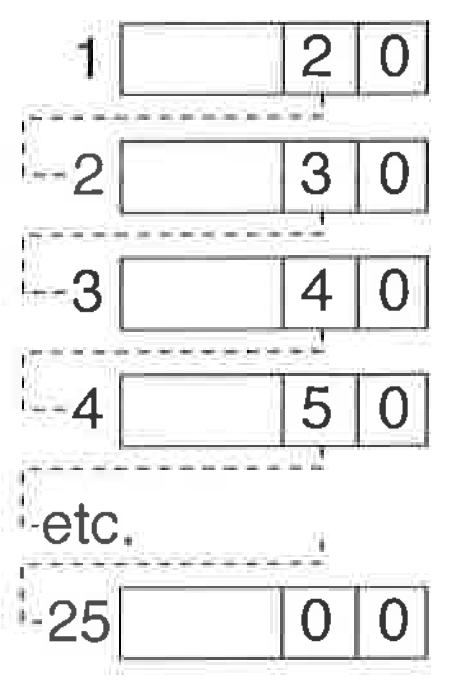
\includegraphics[width=0.125\paperwidth]{C:/Users/Admin/Desktop/Github/question_bank/LyX/static/img/9597-ALVL-2017-P1-Q3-1}
\par\end{center}

\subsubsection*{Task 3.1}

Write the program code to declare the \textbf{empty} data structure
and linked list of 25 unused nodes. Add statement(s) to initiallse
the empty data structure.

\subsubsection*{Evidence 6}

Your program code for Task 3.1. \hfill{}{[}12{]}

This data structure is used to record the possible routes for a robot
to travel from a node A to a node Z. The following data structure
illustrates many possible routes, for example, A$\rightarrow$D$\rightarrow$K$\rightarrow$L$\rightarrow$M$\rightarrow$Z.
It is only possible to move to one of two possible nodes; for example,
from node A, the only move is to node B or node D.
\begin{center}
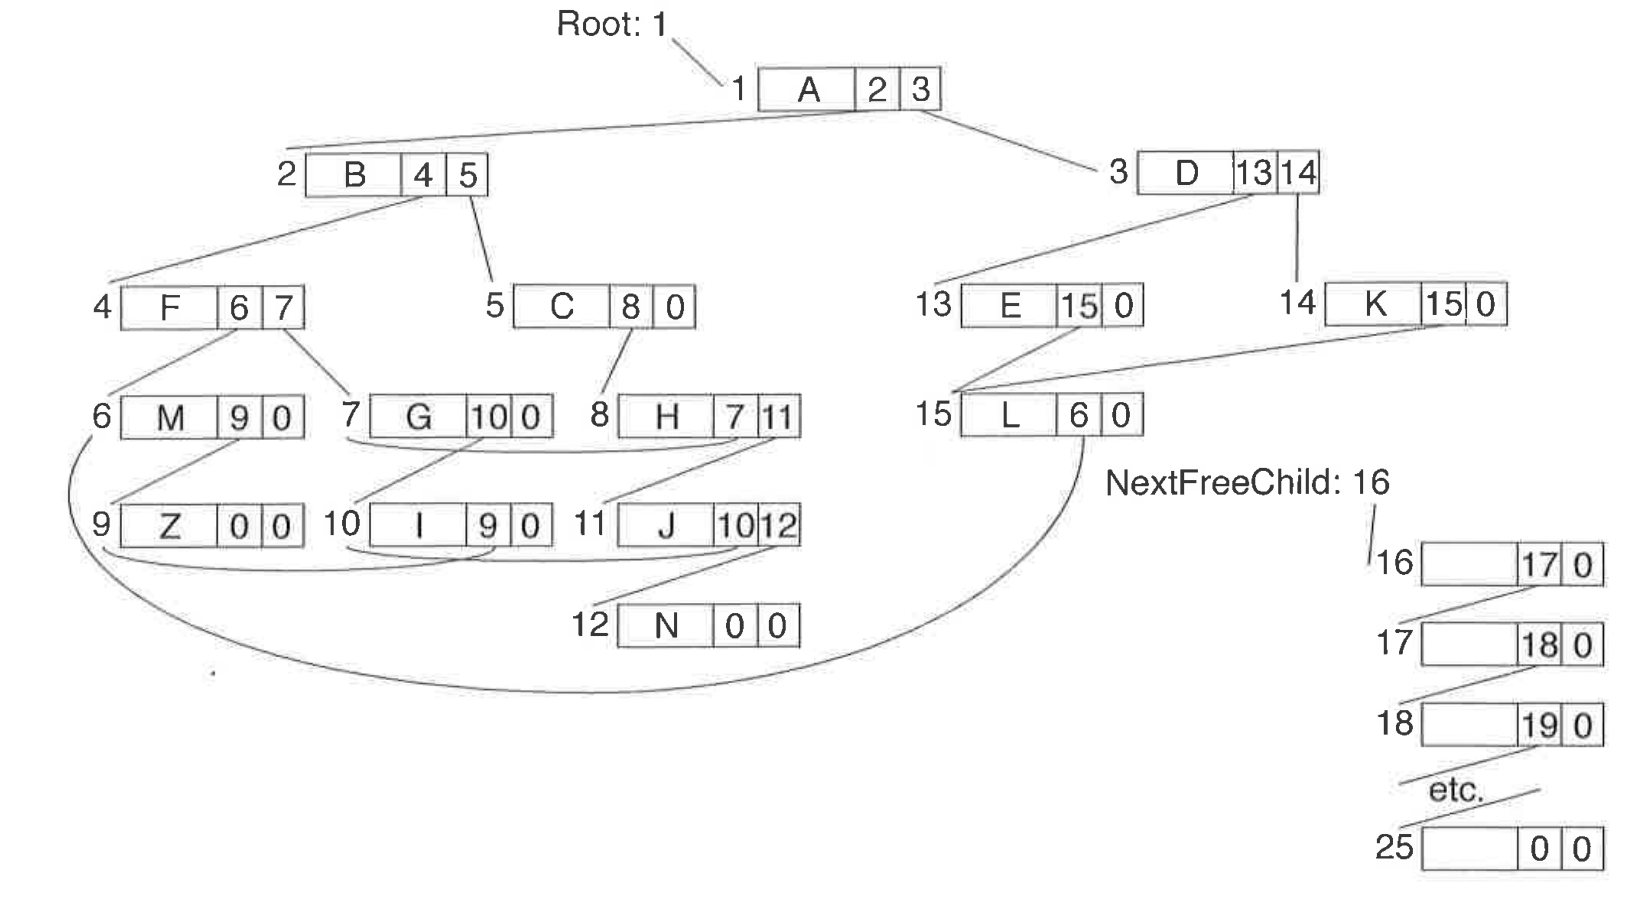
\includegraphics[width=0.5\paperwidth]{C:/Users/Admin/Desktop/Github/question_bank/LyX/static/img/9597-ALVL-2017-P1-Q3-2}
\par\end{center}

This data structure has 15 nodes (A to N and Z) but for future development
a maximum of 25 nodes is specified. All nodes are unique.

The pseudocode on the next page can be used to add a node to the data
structure. The procedure \texttt{AddToRobotData} uses the parameters
\texttt{NewDataItem}, \texttt{ParentItem} and \texttt{ThisMove}.

The parameter \texttt{ThisMove} holds the move made to create this
new item (\textquoteleft L' for LeftChild, \textquoteleft R' for RightChild,
\textquoteleft X\textquoteright{} for initial state/root), and the
\texttt{ParentItem} parameter holds the value of the parent item which
points to this \texttt{NewDataItem}.
\begin{center}
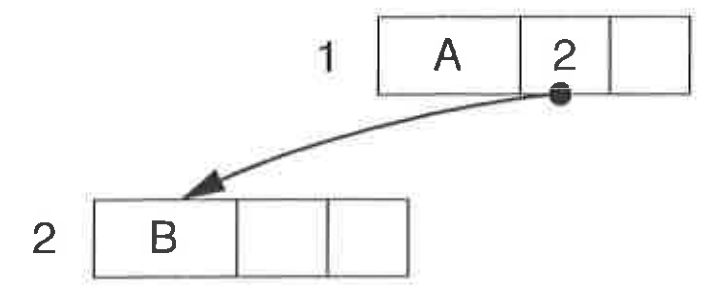
\includegraphics[width=0.25\paperwidth]{C:/Users/Admin/Desktop/Github/question_bank/LyX/static/img/9597-ALVL-2017-P1-Q3-3}
\par\end{center}

To add node B as shown, the procedure call would be \texttt{AddToRobotData
('B', \textquoteleft A', 'L')} . The parameters used would be: 

\texttt{B}, the new node 

\texttt{A}, the parent node 

\texttt{L}, the location of the child (which has an index of 2) is
recorded in \texttt{LeftChild} of A.

The following pseudocode (available in PS EUDOCODE\_TASK\_3\_2 . TXT)
can be used to add a node to the data structure.

\noindent %
\noindent\begin{minipage}[t]{1\columnwidth}%
\texttt{FUNCTION FindNode(NodeValue) RETURNS INTEGER }

\texttt{\qquad{}Found <- FALSE}

\texttt{\qquad{}CurrentPosition <- Root }

\texttt{\qquad{}REPEAT }

\texttt{\qquad{}\qquad{}IF RobotData{[}CurrentPosition{]}.DataValue
= NodeValue THEN }

\texttt{\qquad{}\qquad{}\qquad{}Found <- TRUE }

\texttt{\qquad{}\qquad{}ELSE }

\texttt{\qquad{}\qquad{}\qquad{}CurrentPosition <- CurrentPosition
+ 1 }

\texttt{\qquad{}\qquad{}ENDIF }

\texttt{\qquad{}UNTIL Found = TRUE OR CurrentPosition > 25 }

\texttt{\qquad{}IF CurrentPOSition > 25 THEN }

\texttt{\qquad{}\qquad{}RETURN 0}

\texttt{\qquad{}ELSE }

\texttt{\qquad{}\qquad{}RETURN CurrentPosition }

\texttt{\qquad{}ENDIF }

\texttt{ENDFUNCTION}

\bigskip{}

\texttt{PROCEDURE AddToRobotData(NewDataItem, ParentItem, ThisMove) }

\texttt{\qquad{}\qquad{}IF Root = 1 AND NextFreeChild = 1 THEN }

\texttt{\qquad{}\qquad{}\qquad{}NextFreeChild <- RobocData{[}NextFreeChild{]}.LeftChild }

\texttt{\qquad{}\qquad{}\qquad{}RobotDataIRoot{]}.LeftChild <-
0 }

\texttt{\qquad{}\qquad{}\qquad{}RobotData{[}Root{]}.DataValue <-
NewDataItem }

\texttt{\qquad{}\qquad{}ELSE }

\texttt{\qquad{}\qquad{}\qquad{}// does the parent exist? . }

\texttt{\qquad{}\qquad{}\qquad{}ParentPosition <- FindNode(ParentItem) }

\texttt{\qquad{}\qquad{}\qquad{}IF RarentPosition > 0 THEN // parent
exists }

\texttt{\qquad{}\qquad{}\qquad{}\qquad{}// does the child exist? }

\texttt{\qquad{}\qquad{}\qquad{}\qquad{}ExistingChild <- FindNode(NewDataItem)
' }

\texttt{\qquad{}\qquad{}\qquad{}\qquad{}IF ExistingChild > 0 THEN
// child exists }

\texttt{\qquad{}\qquad{}\qquad{}\qquad{}\qquad{}ChildPointer
<- ExistingChild }

\texttt{\qquad{}\qquad{}\qquad{}\qquad{}ELSE }

\texttt{\qquad{}\qquad{}\qquad{}\qquad{}ChildPointer <- NextFreeChild }

\texttt{\qquad{}\qquad{}\qquad{}\qquad{}NextFreeChild <- RobotDataINextFreeChild\}.LeftChild }

\texttt{\qquad{}\qquad{}\qquad{}\qquad{}RobotData{[}ChildPointer{]}.LeftChild
<- 0 }

\texttt{\qquad{}\qquad{}\qquad{}\qquad{}RobotData{[}ChildPointer{]}.DataValue
<- NewDataItem }

\texttt{\qquad{}\qquad{}\qquad{}\qquad{}ENDIF }

\texttt{\qquad{}\qquad{}\qquad{}\qquad{}IF ThisMove = 'L' THEN }

\texttt{\qquad{}\qquad{}\qquad{}\qquad{}\qquad{}RobotData{[}ParentPosition{]}.LeftChild
<- ChildPointer }

\texttt{\qquad{}\qquad{}\qquad{}\qquad{}ELSE }

\texttt{\qquad{}\qquad{}\qquad{}\qquad{}\qquad{}RobotData{[}ParentPosition{]}.RightChild
<- ChildPointer }

\texttt{\qquad{}\qquad{}\qquad{}\qquad{}ENDIF }

\texttt{\qquad{}\qquad{}\qquad{}ENDIF}\textbf{ }

\texttt{\qquad{}\qquad{}ENDIF }

\texttt{ENDPROCEDURE}%
\end{minipage}

\subsubsection*{Task 3.2}

Write code to implement \texttt{AddToRobotData} and \texttt{FindNode}
from this pseudocode.

You may use the text file \texttt{PSEUDOCODE\_TASK\_3\_2.TXT} as a
basis for writing your code.

\subsubsection*{Evidence 7}

Your program code for Task 3.2. \hfill{}{[}7{]}

\subsubsection*{Task 3.3}

Write a procedure \texttt{OutputData} which displays the value of
\texttt{Root}, the value of \texttt{NextFreeChild} and the contents
of \texttt{RobotData} in index order.

\subsubsection*{Evidence 8}

Your program code for Task 3.3.\hfill{} {[}6{]}

\subsubsection*{Task 3.4}

The file \texttt{SEARCHTREE.TXT} contains the data for the search
tree. Each row of the file contains three comma separated values,
for example, the first row contains '\texttt{A}', '\texttt{0}' and
'X'. The file is organised as: \texttt{NewDataltem, ParentItem, ThisMove}

\texttt{NewDataItem, ParentItem, ThisMove}

\texttt{$\dots$}

\texttt{<End of File>}

There are a total of 20 lines in the \texttt{SEARCHTREE.TXT} file
representing possible routes.

Write a main program to read the contents of this file and use \texttt{AddToRobotData}
and \texttt{FindNode} to insert these routes into \texttt{RobotData}.
Your program will then call the \texttt{OutputData} procedure. 

\subsubsection*{Evidence 9}

Your program code for Task 3.4. \hfill{}{[}6{]}

\subsubsection*{Evidence 10}

Screenshot showing the output from running the program in Task 3.4.\hfill{}
{[}2{]}

\subsubsection*{Task 3.5}

Write a recursive pre-order tree traversal that will display all valid
routes from A to Z by following the routes described in \texttt{RobotData}.

\subsubsection*{Evidence 11}

Your program code for Task 3.5.\hfill{} {[}6{]}

\subsubsection*{Evidence 12}

Screenshot showing the output from running the program in Task 3.5.\hfill{}
{[}1{]}

 \newpage 

\item \textbf{{[}ALVL/9597/2017/P1/Q4{]} }

A computer program can generate a simple Sudoku puzzle using a 4 x
4 two-dimensional array. 

An example of this puzzle is: 
\begin{center}
\begin{tabular}{|c|c|c|c|}
\hline 
4 & 3 & 2 & 1\tabularnewline
\hline 
1 & 2 & 4 & 3\tabularnewline
\hline 
3 & 4 & 1 & 2\tabularnewline
\hline 
2 & 1 & 3 & 4\tabularnewline
\hline 
\end{tabular}
\par\end{center}

The first step to creating this puzzle is to develop a program to
display the 4 x 4 twodimensional array as a grid. This program will
display the grid as: 
\begin{center}
\begin{tabular}{cccc}
4 & 3 & 2 & 1\tabularnewline
1 & 2 & 4 & 3\tabularnewline
3 & 4 & 1 & 2\tabularnewline
2 & 1 & 3 & 4\tabularnewline
\end{tabular}
\par\end{center}

\subsubsection*{Task 4.1}

Create a program design that will declare, initialise and display
the example puzzle shown. This design will: 
\begin{itemize}
\item make use of top-down design 
\item include the data structure to represent the puzzle as a grid 
\item initialise the grid using the values shown
\item make use of appropriate procedures and/or functions. 
\end{itemize}

\subsubsection*{Evidence 13}

Your program design for Task 4.1. \hfill{}{[}6{]}

\subsubsection*{Task 4.2}

Write program code to display the puzzle designed in Task 4.1. 

\subsubsection*{Evidence 14}

Your program code.\hfill{} {[}5{]}

\subsubsection*{Evidence 15}

Screenshot of the displayed grid. \hfill{}{[}1{]}

The puzzle is said to be valid if it follows these rules:
\begin{itemize}
\item It consists of tour quadrants.
\item The numbers in each quadrant must add up to ten.
\item Each horizontal and vertical row of the puzzle must also add up to
ten.
\item No number can be repeated in the same row, same column or same quadrant
of the puzzle. 
\end{itemize}
A good strategy tor creating puzzles is to start with a valid \textquoteleft base'
puzzle and perform transformations on it to create new puzzles.

You will write program code to create new valid puzzles. 

Each puzzle created will have two randomly selected transformations.
from a possible four, performed on it. The following are the four
possible transformations that can be carried out. 
\begin{center}
\begin{tabular}{|c|>{\raggedright}p{0.3\columnwidth}|l|}
\hline 
\textbf{Transformation} & \texttt{\hspace{0.05\columnwidth}}Explanation & \multicolumn{1}{l}{}\tabularnewline
\hline 
\textbf{1} & Swaps two rows in the same quadrants & \tabularnewline
 &  & 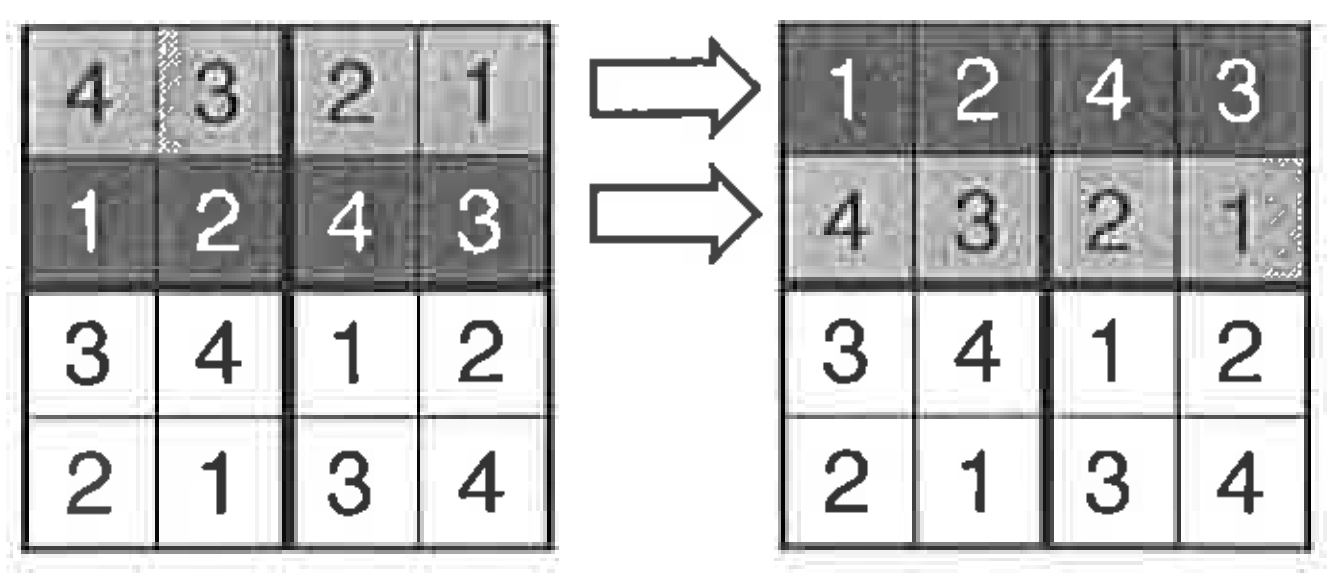
\includegraphics[width=0.3\paperwidth]{C:/Users/Admin/Desktop/Github/question_bank/LyX/static/img/9597-ALVL-2017-P1-Q4-1}\tabularnewline
\hline 
\textbf{2} & Swaps two columns in the same quadrants & \tabularnewline
 &  & 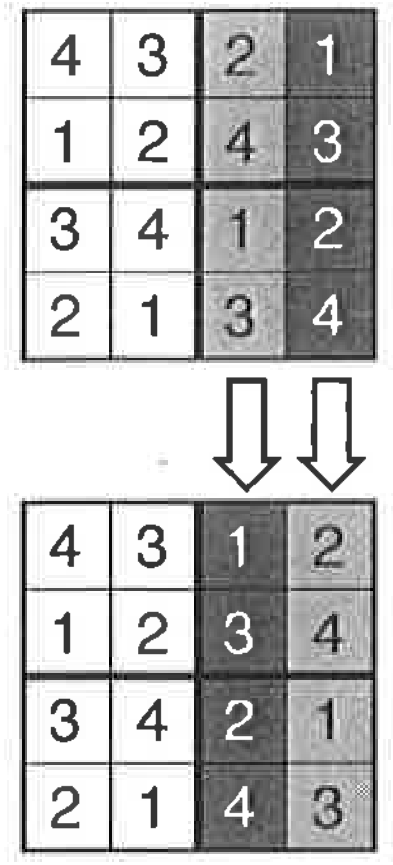
\includegraphics[width=0.15\paperwidth]{C:/Users/Admin/Desktop/Github/question_bank/LyX/static/img/9597-ALVL-2017-P1-Q4-2}\tabularnewline
\hline 
\textbf{3} & Swaps the top and bottom quadrant rows entirely & \tabularnewline
 &  & 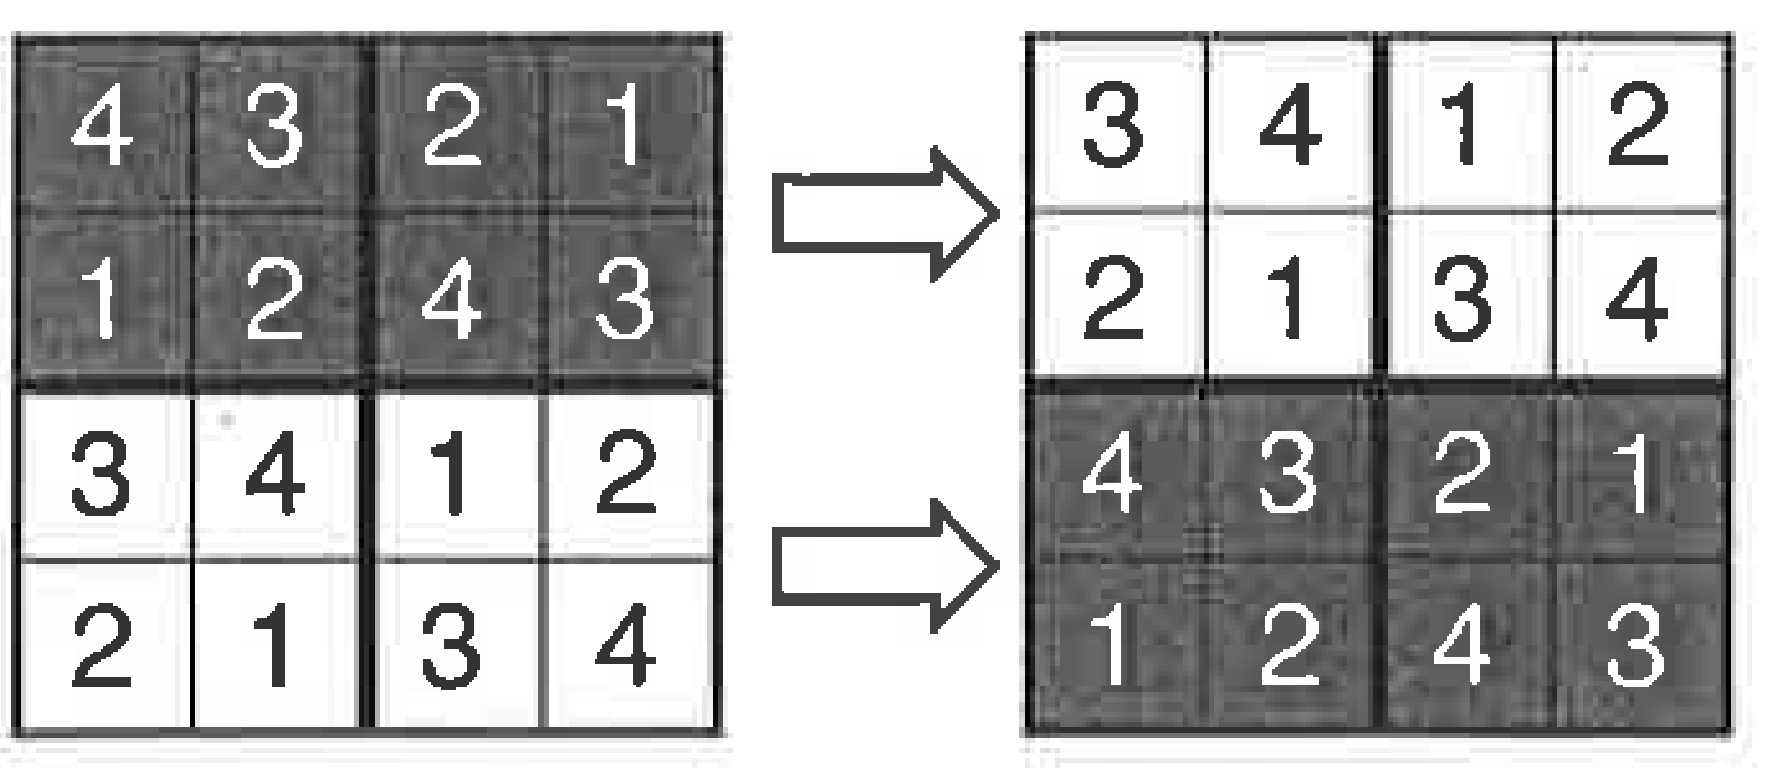
\includegraphics[width=0.3\paperwidth]{C:/Users/Admin/Desktop/Github/question_bank/LyX/static/img/9597-ALVL-2017-P1-Q4-3}\tabularnewline
\hline 
\textbf{4} & Swaps the left and right quadrant columns entirely & \tabularnewline
 &  & 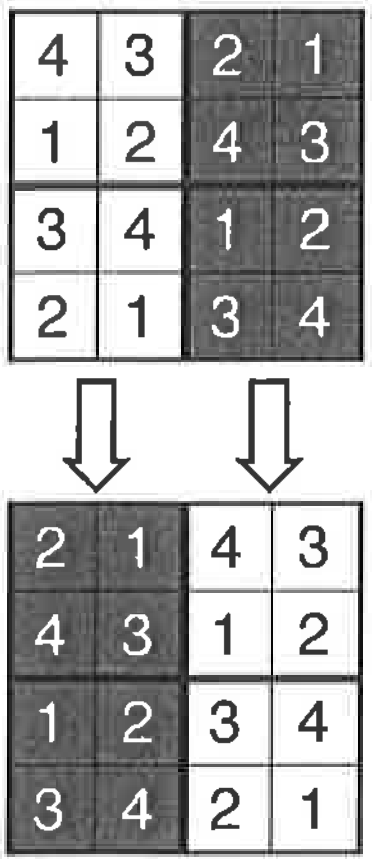
\includegraphics[width=0.15\paperwidth]{C:/Users/Admin/Desktop/Github/question_bank/LyX/static/img/9597-ALVL-2017-P1-Q4-4}\tabularnewline
\hline 
\end{tabular}
\par\end{center}

\subsubsection*{Task 4.3}

Write additional program code with brief \textbf{internal commentary}
to identify each transformation. 

The program code will: 
\begin{itemize}
\item create a method of selecting. at random, two of the four possible
transformations to be applied to the puzzle 
\item call a sub-program for each of the required transformations 
\item randomly select which rows will be transformed for transformations
1 and 2. for example. either the top or bottom two rows (for transformation
1) OR either the left-most or right-most two columns (for transformation
2) respectively 
\item display the puzzle before each transformation is applied and after
the final transformation. Before each transformation. it will also
display the name of the transformation being carried out. 

For example: 

\texttt{4321 }

\texttt{1243 }

\texttt{3412 }

\texttt{2134 }

\texttt{Transformation 1: Swaps two rows in the same quadrants }

\texttt{1243 }

\texttt{4321 }

\texttt{3412 }

\texttt{2134 }

\texttt{Transformation 4: Swaps the left and right quadrant columns
entirely }

\texttt{4312 }

\texttt{2143 }

\texttt{1234 }

\texttt{3421 }
\end{itemize}

\subsubsection*{Evidence 16}

Your program code that includes internal commentary.\hfill{} {[}14{]}

\subsubsection*{Evidence 17}

Screenshots of the output that shows each of the four transformations
applied. \hfill{}{[}4{]}

 \newpage 

\item \textbf{{[}ALVL/9597/2017/P2/Q1{]} }

The principal of a college decides to improve security access. Currently,
the staff use keys to enter classrooms and laboratories. One of the
principal\textquoteright s suggested improvements is to replace the
existing locks and keys with a swipe card system. The principal plans
to purchase swipe card readers for every room, and staff will be issued
with their own swipe card. if a valid card is swiped through a particular
reader, the corresponding door will be unlocked.

Software for controlling the system is required to: 
\begin{itemize}
\item define the rooms that can be entered by each card. The office staff
will make any changes. 
\item produce a pop-up screen on the office staff's computer if an unauthorised
card is used to attempt an entry into a room. 
\item produce reports. Some of the reports will be confidential and can
only be viewed by the principal. 
\end{itemize}
A local software company is selected to produce the software. The
company assigns a development team to the project. 
\begin{enumerate}
\item A systems analyst from the team makes an initial visit to the college. 

State two groups of staff that the systems analyst would need to interview.
Justify your answer. \hfill{}{[}4{]}
\item As a result of the analysis carried out. a diagram is used to show
entities and data flow. Draw a suitable diagram. \hfill{}{[}6{]}
\item The next stage of system development is software design.
\begin{enumerate}
\item Describe the checks that the team needs to make at the end of this
stage. \hfill{}{[}2{]}
\item Describe two methods that could be used to check this design. For
each method, identify the members of the development team involved
other than the systems analyst. {[}6{]}
\end{enumerate}
\item The swipe card system will need to be fully tested. The company carries
out white box and black box testing. 

Explain \textbf{three} differences between black box and white box
testing. \hfill{}{[}6{]}
\item User documentation will be produced during the development process. 

Describe \textbf{three} sections that should be included in the user
guide for this system.\hfill{} {[}6{]}
\item After the system is implemented, maintenance will be required. 

Name and describe \textbf{two} types of maintenance. For each type,
give an example for the swipe card system. \hfill{}{[}6{]}
\item Describe a method that can be used to ensure that only the office
staff can change the system and only the principal can view confidential
reports. \hfill{}{[}2{]}
\item The principal is considering expanding the use of the swipe card system
to record attendance in classes. 

Describe \textbf{one} disadvantage of this proposal and suggest a
more reliable method.\hfill{} {[}2{]}
\end{enumerate}

 \newpage 

\item \textbf{{[}ALVL/9597/2017/P2/Q2{]} }

A multinational company has many local branches in various parts of
the country that are linked using a wide area network (WAN). 
\begin{enumerate}
\item The company's network transfers data using asynchronous data transmission. 
\begin{enumerate}
\item State which of the following diagrams represents asynchronous data
transmission. Explain your answer. \hfill{}{[}2{]}
\begin{center}
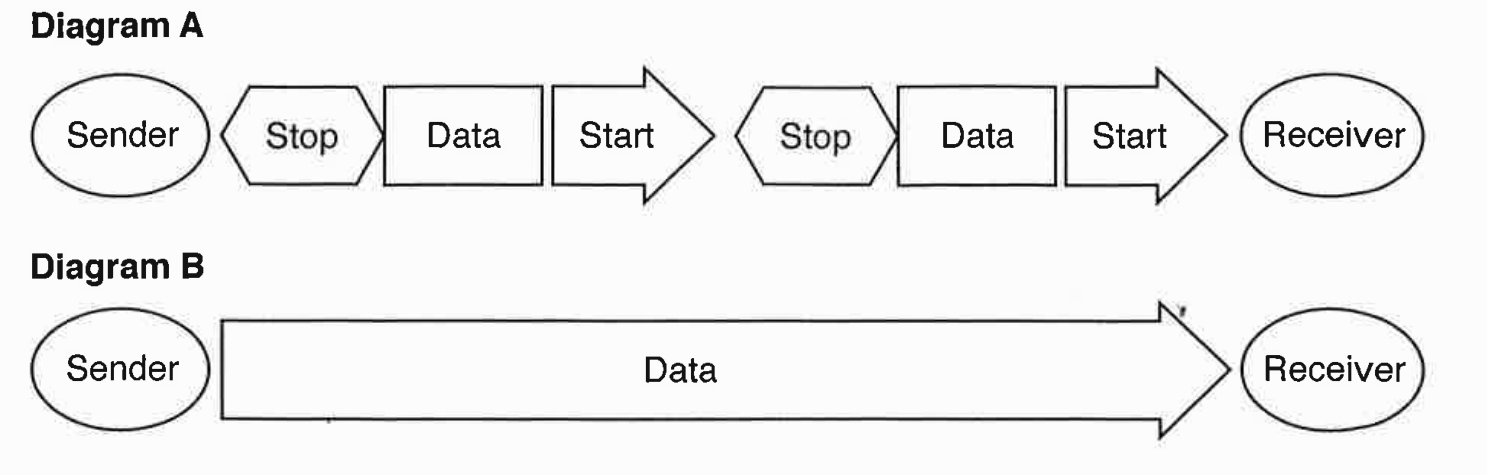
\includegraphics[width=0.5\paperwidth]{C:/Users/Admin/Desktop/Github/question_bank/LyX/static/img/9597-ALVL-2017-P2-Q2-1}
\par\end{center}
\item Explain why asynchronous data transmission affects network performance.\hfill{}
{[}2{]}
\end{enumerate}
\end{enumerate}
An employee works from home on her wireless laptop. The following
diagram shows the configuration of the employee's home network.
\begin{center}
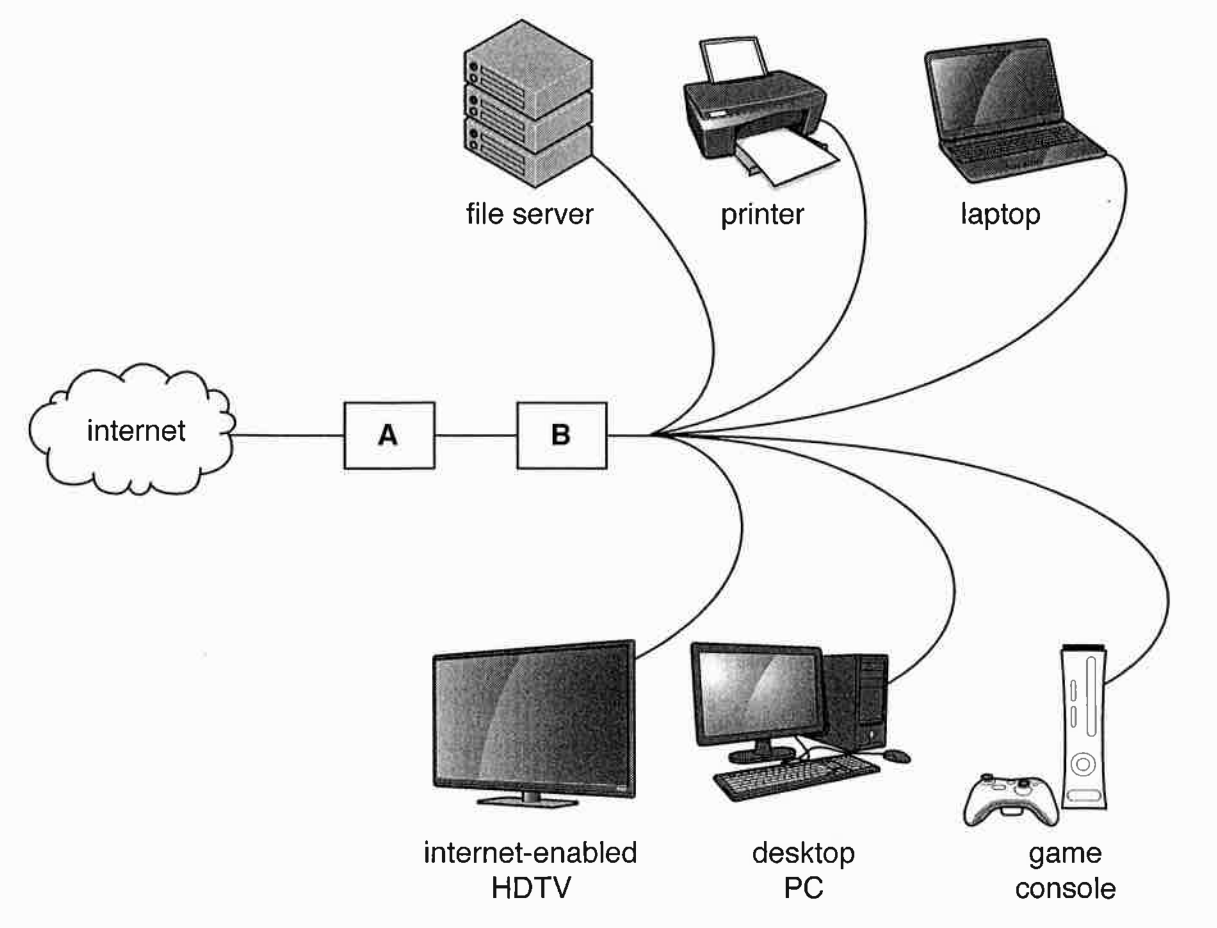
\includegraphics[width=0.5\paperwidth]{C:/Users/Admin/Desktop/Github/question_bank/LyX/static/img/9597-ALVL-2017-P2-Q2-2}
\par\end{center}
\begin{enumerate}
\item[(b)] This network uses both a switch and a router to transfer data. State
which of the pieces of equipment labelled \textbf{A} and \textbf{B}
is the switch. Explain your answer. \hfill{}{[}2{]}
\item[(c)] Describe \textbf{two} features of a router.\hfill{} {[}2{]}
\item[(d)] Describe \textbf{one} advantage and \textbf{one} disadvantage. for
the employee, of working from home.\hfill{} {[}2{]}
\end{enumerate}

 \newpage 

\item \textbf{{[}ALVL/9597/2017/P2/Q3{]} }
\begin{enumerate}
\item Explain what is meant by an object in object-oriented programming.
.\hfill{}{[}2{]} 
\item {} 
\begin{enumerate}
\item A student is writing a program to represent people in a university.
Tutors, office workers, lecturers and professors are all employed
by the university. A professor is a senior lecturer. The university
educates both undergraduate and graduate students. 

The student\textquoteright s program contains a class with the identifier
\texttt{Person}. Sub-classes share the characteristics of this class. 

Copy and complete the following inheritance diagram by adding sub-classes
\texttt{Professor}, 

\texttt{OfficeWorker}, \texttt{Lecturer}, \texttt{Undergraduate},
\texttt{Staff}, \texttt{Graduate}, \texttt{Student} and \texttt{Tutor}.
\hfill{}{[}2{]} 
\begin{center}
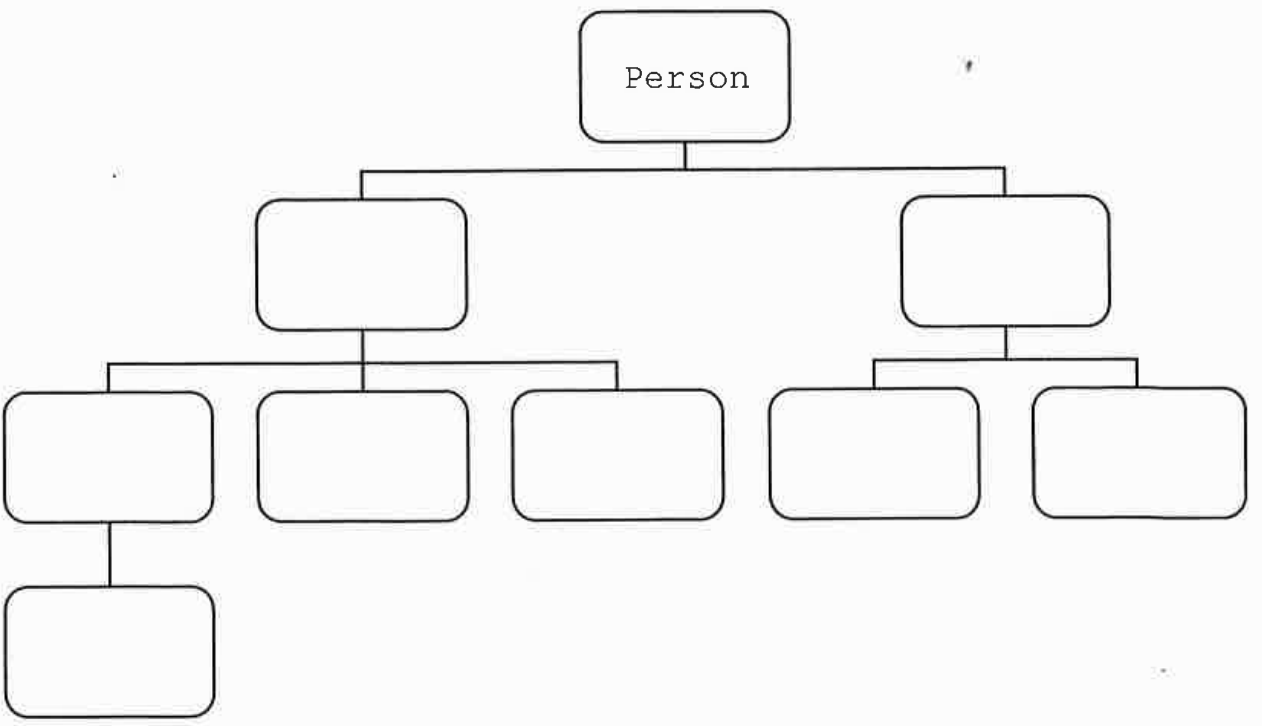
\includegraphics[width=0.5\paperwidth]{C:/Users/Admin/Desktop/Github/question_bank/LyX/static/img/9597-ALVL-2017-P2-Q3}
\par\end{center}
\item Explain why inheritance is an important feature of object-oriented
programming.\hfill{}{[}2{]} 
\end{enumerate}
\item A stack is a data structure that can be implemented in object-oriented
programming. The implementation of a stack requires an integer variable
and an array. 
\begin{enumerate}
\item Describe the purpose of the integer variable in the implementation
of a stack class.\hfill{} {[}1{]}
\item Describe the purpose of the array in the implementation of a stack
class.\hfill{} {[}1{]}
\item Explain how to use the stack data structure to compute the following
expression: 
\noindent \begin{center}
$\left(\text{A}+\text{B}\right)\times\left(\text{C}+\text{D}\right)$\hfill{}
{[}2{]}
\par\end{center}

\end{enumerate}
\end{enumerate}

 \newpage 

\item \textbf{{[}ALVL/9597/2017/P2/Q4{]} }
\begin{enumerate}
\item A local area network (LAN) can be set up as either client-server or
peer-to-peer. 
\begin{enumerate}
\item State where data are stored on a client-server network. \hfill{}
{[}1{]}
\item State where data are stored on a peer-to-peer network. \hfill{} {[}1{]}
\item Describe \textbf{one} benefit of a client-server network over a peer-to-peer
network. \hfill{} {[}2{]}
\item Describe \textbf{one} drawback of a client-server network compared
to a peer-to-peer network.\hfill{} {[}2{]}
\end{enumerate}
\item A college has five IT rooms. Each room has 20 computers which can
only print to a single printer in the room. At busy times in the year,
there can be up to 100 students printing their coursework at the same
time. \textquoteleft 0

Explain how all these print jobs are controlled and sent to the printer.\hfill{}
{[}2{]}
\item A 30 megabyte file is transferred over a network to a printer in 5
seconds. 

Calculate the transfer rate, in megabits per second, used to transfer
this file. Show all of your working. \hfill{} {[}2{]}
\end{enumerate}

 \newpage 

\item \textbf{{[}ALVL/9597/2017/P2/Q5{]} }The following grid shows the initial
state of a popular puzzle.
\begin{center}
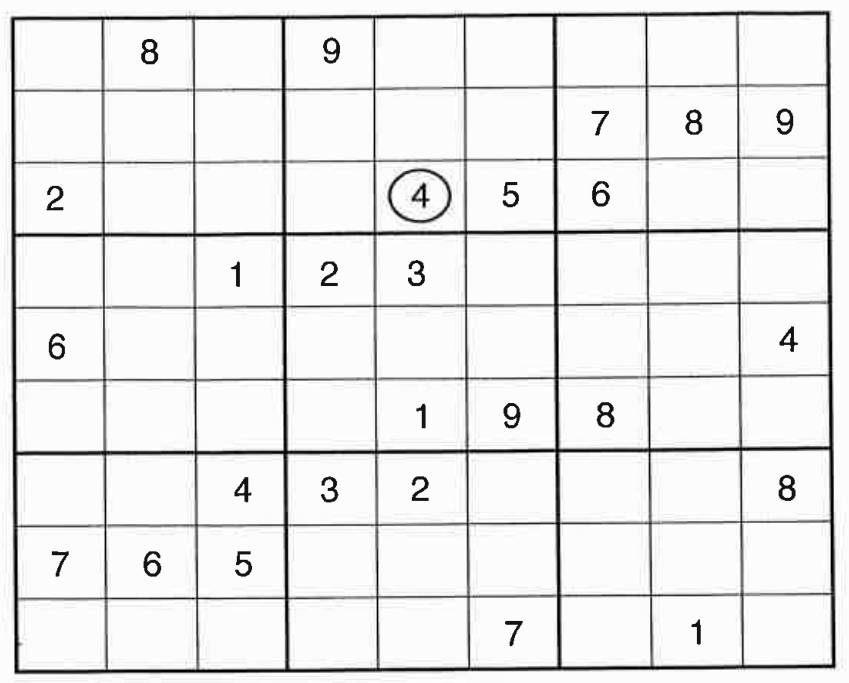
\includegraphics[width=0.5\paperwidth]{C:/Users/Admin/Desktop/Github/question_bank/LyX/static/img/9597-ALVL-2017-P2-Q5}
\par\end{center}

The aim of the puzzle is to fill the whole grid so that every row,
every column and every $3\times3$ mini-grid contains a number between
1 and 9. No number should be repeated in any row, column or 3 x 3
minigrid. 

A software company is creating an online version of the puzzle. A
programmer is asked to create the puzzle software. 
\begin{enumerate}
\item The programmer decides to use a 2D array to store the puzzle.
\begin{enumerate}
\item Copy and complete the following line of pseudocode. 

\texttt{DECLARE Puzzle ARRAY{[}1 : ...., .... : ....{]} OF ......................}
\hfill{}{[}2{]}

The circled value in the diagram above needs to be assigned to the
appropriate array element. 
\item Copy and complete the following line of pseudocode. 

\texttt{Puzzle{[}...., ....{]} <- ...............................}
\hfill{}{[}2{]}
\item Explain why a 2D array is more suitable than a single 1D array to
represent this puzzle. \hfill{}{[}2{]}
\end{enumerate}
\item The puzzle grid can be saved by writing the array \texttt{Puzzle}
to a file. 

Design an algorithm, using pseudocode, to write the array to the file.
\hfill{} {[}5{]}
\item During the testing of the puzzle software, several errors are discovered. 

Describe \textbf{two} debugging techniques that could be used to locate
these errors. \hfill{}{[}4{]}
\end{enumerate}

 \newpage 

\item \textbf{{[}ALVL/9597/2017/P2/Q6{]} }

A computer company has several offices throughout the country, each
with several salespersons. A record of the sales made by each salesperson
has been set up using a relational database. There is a minimum amount
of \$150 for each sale.

The following tables hold the data. 

\texttt{CUSTOMER (}\texttt{\uline{CustomerID}}\texttt{, CustomerName,
CustomerEmail, CustomerTelephone) }

\texttt{OFFICE (}\texttt{\uline{OfficeID}}\texttt{, Address, Telephone) }

\texttt{SALE (}\texttt{\uline{CustomerID{*}}}\texttt{, }\texttt{\uline{SalesPersonID{*}}}\texttt{,
SaleDate, Amount) }

\texttt{SALESPERSON (}\texttt{\uline{SalesPersonID}}\texttt{, SalespersonName,
OfficeID{*}) }

\textbf{Note:} underline indicates primary key. An asterisk ({*})
indicates a foreign key. 
\begin{enumerate}
\item Draw an Entity-Relationship (E-Fl) diagram to represent the data model.
\hfill{} {[}3{]} 
\item (b) The following is a section of the data dictionary for the data
model. it has three missing entries labelled \textbf{A}, \textbf{B
}and \textbf{C}.
\begin{center}
\begin{tabular}{|l|l|l|c|}
\hline 
\texttt{\textbf{\hspace{0.01\columnwidth}}}\textbf{Table} & \texttt{\textbf{\hspace{0.01\columnwidth}}}\textbf{Field} & \textbf{Data type} & \textbf{Validation}\tabularnewline
\hline 
\texttt{CUSTOMER} & \texttt{CustomerID} & Integer & Unique\tabularnewline
\hline 
\texttt{SALE} & \texttt{CustomerID} & Integer & \textbf{A}\tabularnewline
\hline 
\texttt{SALE} & \texttt{SaleData} & Date & \tabularnewline
\hline 
\texttt{SALE} & \texttt{Amount} & \texttt{\textbf{\hspace{0.01\columnwidth}}}\textbf{B} & \textbf{C}\tabularnewline
\hline 
\end{tabular}
\par\end{center}

State a suitable entry for \textbf{A}, \textbf{B} and \textbf{C}.
\hfill{}{[}3{]} 
\item There is an address field in this database.

Explain why storing the address as a single field is not good database
design. \hfill{}{[}3{]}
\end{enumerate}
Each month, a report is produced to show the sales for each salesperson.
The following is a report for salesperson, B Chin. 
\begin{center}
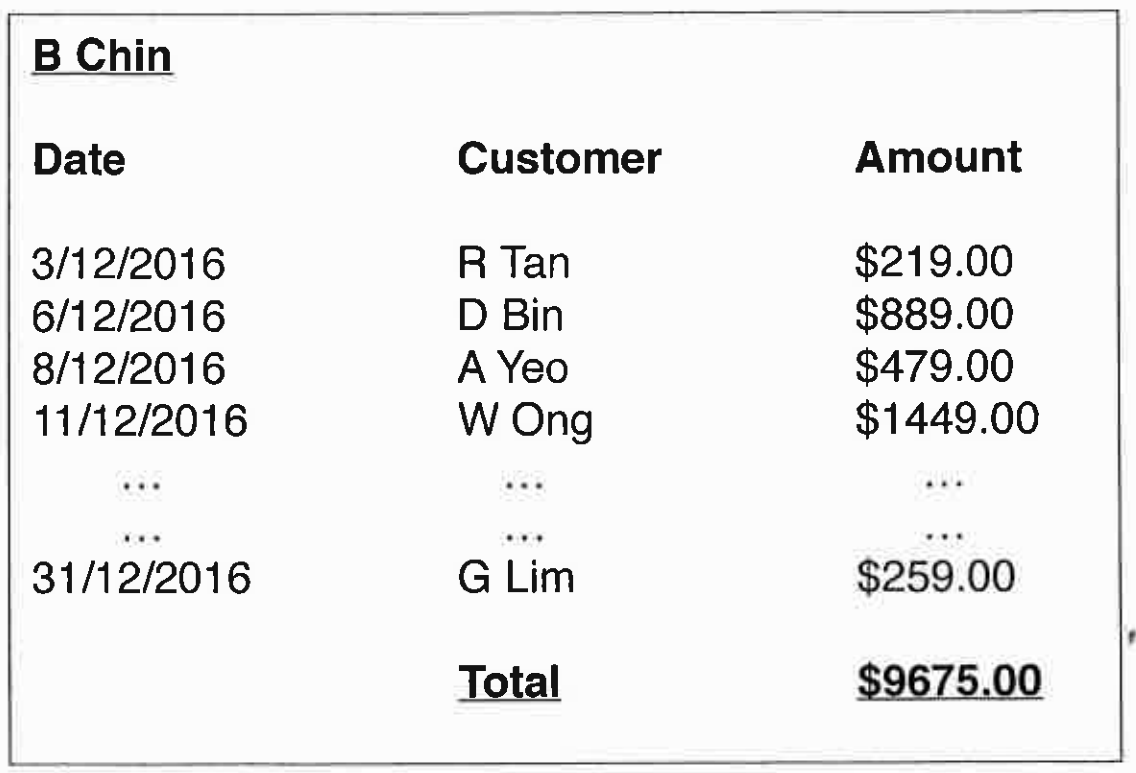
\includegraphics[width=0.5\paperwidth]{C:/Users/Admin/Desktop/Github/question_bank/LyX/static/img/9597-ALVL-2017-P2-Q6}
\par\end{center}
\begin{enumerate}
\item[(d)] {}
\begin{enumerate}
\item To produce the report, the database uses the \texttt{SaleDate} and
\texttt{Amount} fields in the \texttt{SALE} table. 

Name \textbf{four }other fields that the database uses to produce
this report.\hfill{} {[}4{]}
\item State \textbf{two} features of a relational database management system
which would be used to calculate and display the total for this salesperson.\hfill{}
{[}2{]}
\end{enumerate}
\end{enumerate}

 \newpage 

\item \textbf{{[}HCI/PRELIM/9597/2017/P1/Q1{]} }

A web log,\texttt{ WEBLOG.txt}, keeps track of the date and time the
server is being accessed, and the client that accessed it. The client
is identified by either the host name or internet address. The format
of \texttt{WEBLOG.txt} is as follows: 
\noindent \begin{center}
\texttt{<host name>|<DD/MMM/YYYY:HH:MM:SS> }
\par\end{center}

or
\noindent \begin{center}
\texttt{<internet address>|<DD/MMM/YYYY:HH:MM:SS> }
\par\end{center}

Below is a sample of \texttt{WEBLOG.txt}: 

\noindent\fbox{\begin{minipage}[t]{1\columnwidth - 2\fboxsep - 2\fboxrule}%
\texttt{199.72.81.55|01/Jul/1995:00:00:01 }

\texttt{unicomp6.unicomp.net|01/Jul/1995:00:00:06 }

\texttt{199.120.110.21|01/Jul/1995:00:00:09 }

\texttt{burger.letters.com|01/Jul/1995:00:00:11} %
\end{minipage}}

The client address (host name or internet address) can appear multiple
times, depending on how many times it accessed the server. Similarly,
the date it accessed the server can be duplicated too because it can
access the server many times in a day. 

A summary report, SUMMARY.txt, is to be generated to list the \textbf{unique}
clients (hosts name/internet address) and the corresponding list of
\textbf{unique} dates that it has accessed the server, from the web
log, \texttt{WEBLOG.txt}. 

Below is a sample of \texttt{SUMMARY.txt}: 

\noindent\fbox{\begin{minipage}[t]{1\columnwidth - 2\fboxsep - 2\fboxrule}%
\texttt{199.72.81.55 01/Jul/1995,03/Jul/1995,04/Jul/1995 }

\texttt{Buger.letters.com 01/Jul/1995,05/Jul/1995}

\texttt{Computing.com 01/Jul/1995,02/Jul/1995,03/Jul/1995}%
\end{minipage}}

\subsection*{Task 1.1}

Write a procedure \texttt{ReadLog()} to read \texttt{WEBLOG.txt},
using a suitable data structure(s), and prepare the log information
to create \texttt{SUMMARY.txt}.

\subsection*{Evidence 1 }

Your \texttt{ReadLog()} procedure code. \hfill{}{[}4{]}

\subsection*{Task 1.2 }

Write a procedure \texttt{ProcessLog()} to generate \texttt{SUMMARY.txt}. 

\subsection*{Evidence 2}

Your \texttt{ProcessLog()} procedure code.\hfill{} {[}4{]}

\subsection*{Evidence 3 }

Screenshot of \texttt{SUMMARY.txt} after running the program. \hfill{}{[}1{]}

\subsection*{Task 1.3 }

Add code to your Task 1.2 program to output to screen the highest
number of days the server was accessed by any client, and the corresponding
client(s). Below is a sample of screen output:

\noindent\begin{minipage}[t]{1\columnwidth}%
\texttt{Highest frequency (days): 3 }

\texttt{Accessed by: }

\texttt{199.72.81.55}

\texttt{Computing.com}%
\end{minipage}

\subsection*{Evidence 4}

Your program code for Task 1.3.\hfill{} {[}4{]}

\subsection*{Evidence 5}

Screenshot of the program output. \hfill{}{[}1{]}

 \newpage 

\item \textbf{{[}HCI/PRELIM/9597/2017/P1/Q2{]} }

The files \texttt{CUPS-SOLD1.txt} and \texttt{CUPS-SOLD2.txt} contain
the daily total number of cups of coffee sold at a caf� over a period
of 50 days. The task is to read the daily sales from the file and
to allow a search for a specific sales figure. You will program two
different search algorithms: 
\begin{itemize}
\item Linear Search 
\item Binary Search 
\end{itemize}

\subsection*{Task 2.1 }

Write program code that repeatedly: 
\begin{itemize}
\item displays a menu with the following options:
\noindent \begin{center}
\begin{tabular}{|l|}
\hline 
1. Read File\tabularnewline
2. Linear Search\tabularnewline
3. Binary Search\tabularnewline
4. End\tabularnewline
\hline 
\end{tabular}
\par\end{center}
\item calls an appropriate procedure/function depending on the user\textquoteright s
option.
\end{itemize}

\subsection*{Evidence 6 }

Program code for Task 2.1. \hfill{}{[}3{]}

\subsection*{Task 2.2 }

Write the program code for a procedure to implement menu option 1. 

\subsection*{Evidence 7 }

Program code for menu option 1. \hfill{}{[}2{]}

Options 2 and 3 will perform a search for a specified sales figure
and display a message to indicate if it is found or not. 

\subsection*{Task 2.3}

Write program code as a function to implement the linear search for
menu option 2. The function will return 0 if the sales figure is found,
or -1 if it is not found. 

The program will: 
\begin{itemize}
\item Input a sales figure 
\item Use the function \texttt{LinearSearch} 
\item Report whether or not this sales figure was found.
\end{itemize}
Use \texttt{CUPS-SOLD1.txt} to test your program code. 

Run the program two times. Use the following inputs: \texttt{167}
and \texttt{405}. 

\subsection*{Evidence 8}
\begin{itemize}
\item Program code for menu option 2.
\item Screenshots showing the output from menu option 2. \hfill{}{[}5{]}
\end{itemize}

\subsection*{Task 2.4 }

Write program code as a function to implement the binary search for
menu option 3. The function will return \texttt{0} if the sales figure
is found, or \texttt{-1} if it is not found. 

\textbf{{*}Hint: Do not use any pre-defined sort function e.g. sort()
in your program code.}

The program will: 
\begin{itemize}
\item Input a sales figure
\item Use the function \texttt{BinarySearch} 
\item Report whether or not this sales figure was found.
\end{itemize}
Use \texttt{CUPS-SOLD1.txt} to test your program code. Run the program
two times. Use the following inputs: \texttt{366} and \texttt{123}. 

\subsection*{Evidence 9 }
\begin{itemize}
\item Program code for menu option 3. 
\item Screenshots showing the output from menu option 3. \hfill{}{[}10{]}
\end{itemize}

\subsection*{Task 2.5}

Amend your program code for the linear search function so that if
the specified sales figure exists, the number of day(s) with this
sales figure is also reported. 

Use the file \texttt{CUPS-SOLD2.txt} to test your program. 

\subsection*{Evidence 10 }

The amended program code for menu option 2. \hfill{}{[}3{]}

\subsection*{Task 2.6}

Study the contents of \texttt{CUPS-SOLD2.txt} and then devise a set
of three test cases with the sales figures to be used for testing
the amended code. Evidence 11 A screenshot for each test case you
considered. Annotate the screenshot explaining the purpose of each
test. \hfill{}{[}3{]}

 \newpage 

\item \textbf{{[}HCI/PRELIM/9597/2017/P1/Q3{]} }

An application is to be created to store a Football League table data.
The team names are stored in the file \texttt{TEAMS.txt}. The results
of the football matches are provided in file \texttt{RESULTS.txt}.

Each match data takes up one line, for example: \texttt{MadUnited
2 Chelsand 1 }

That is, \texttt{MadUnited} won \texttt{Chelsand}, scoring two goals
and conceding one goal, or Chelsand lost to Mad United, scoring one
goal and conceding two goals. 

The League table that needs to be created has the following information: 
\noindent \begin{center}
\begin{tabular}{llllllllll}
\textbf{Team} &  & \textbf{P} & \textbf{W} & \textbf{D} & \textbf{L} & \textbf{GF} & \textbf{GA} & \textbf{GD} & \textbf{Points}\tabularnewline
\hline 
\texttt{MadUnited} &  & \texttt{4} & \texttt{3} & \texttt{1} & \texttt{0} & \texttt{8} & \texttt{3} & \texttt{5} & \texttt{10}\tabularnewline
\texttt{Chelsand} &  & \texttt{4} & \texttt{2} & \texttt{1} & \texttt{1} & \texttt{10} & \texttt{7} & \texttt{3} & \texttt{7}\tabularnewline
\texttt{Lovepool} &  & \texttt{5} & \texttt{2} & \texttt{1} & \texttt{2} & \texttt{4} & \texttt{6} & \texttt{-2} & \texttt{7}\tabularnewline
$\dots$ &  &  &  &  &  &  &  &  & \tabularnewline
$\dots$ &  &  &  &  &  &  &  &  & \tabularnewline
\end{tabular}
\par\end{center}

\noindent %
\noindent\begin{minipage}[t]{1\columnwidth}%
\textbf{Legend}: 

\textbf{P} -- games played 

\textbf{W} -- games won

\textbf{D} -- games drawn

\textbf{L} -- games lost 

\textbf{GF} -- goals for (scored against opponents)

\textbf{GA} -- goals against (goals conceded by team)

\textbf{GD} -- goal difference, i.e. GD = GF -- GA

\textbf{Points} -- computed based on 3 points per win, 1 point per
draw and zero points per loss%
\end{minipage}

\subsection*{Task 3.1 }

Write program code for a procedure \texttt{CreateUpdateFile} which
does the following: 
\begin{itemize}
\item the program reads the \textbf{first} match results from \texttt{RESULTS.txt}
\item appends to the results of each team to a text file \texttt{NEWFILE.txt}
with the following information: team name, result of match (W/D/L),
goals for (GF), goals against (GA)
\item for e.g. the data \textquotedblleft \texttt{MadUnited 2 Chelsand 1}\textquotedblright{}
will result in the following two records to be appended to \texttt{NEWFILE.txt}.

\noindent\begin{minipage}[t]{1\columnwidth}%
\texttt{MadUnited,W,2,1}

\texttt{Chelsand,L,1,2}%
\end{minipage}
\end{itemize}

\subsection*{Evidence 12 }

Your CreateUpdateFile program code. \hfill{}{[}5{]}

\subsection*{Task 3.2 }

Amend your \texttt{CreateUpdateFile} program code from Task 3.1 so
that all the match results are read from \texttt{RESULTS.txt}, and
the \texttt{NEWFILE.txt} updated accordingly. 

\subsection*{Evidence 13 }

Your program code for the amended procedure \texttt{CreateUpdateFile}.
\hfill{}{[}2{]}

\subsection*{Evidence 14 }

2 screenshots of \texttt{NEWFILE.txt} showing first 10 and last 10
records. \hfill{} {[}2{]}

\subsection*{Task 3.3 }

Write program code for a function \texttt{ComputeTeamStat} which does
the following: 
\begin{itemize}
\item receives a team name as a parameter 
\item the function searches the file \texttt{NEWFILE.txt} for all occurrences
of that team
\item calculates and outputs the team\textquoteright s league table information, 

e.g. for team \textquoteleft \texttt{MadUnited}\textquoteright , it
may output the following: 
\noindent \begin{center}
\begin{tabular}{llllllllll}
\textbf{Team} &  & \textbf{P} & \textbf{W} & \textbf{D} & \textbf{L} & \textbf{GF} & \textbf{GA} & \textbf{GD} & \textbf{Points}\tabularnewline
\hline 
\texttt{MadUnited} &  & \texttt{4} & \texttt{3} & \texttt{1} & \texttt{0} & \texttt{8} & \texttt{3} & \texttt{5} & \texttt{10}\tabularnewline
\end{tabular}
\par\end{center}
\end{itemize}

\subsection*{Evidence 15 }

Your \texttt{ComputeTeamStat} program code.\hfill{} {[}6{]}

\subsection*{Evidence 16 }

A screenshot showing the output for the team \texttt{Everlong}. \hfill{}{[}1{]}

\subsection*{Task 3.4 }

Write program code for a procedure \texttt{GenerateTable} which does
the following: 
\begin{itemize}
\item reads the data from files \texttt{TEAMS.txt} and \texttt{NEWFILE.txt}
\item and makes use of the function \texttt{ComputeTeamStat} from Task 3.3 
\item to output the complete league table information ordered by the team
with the highest points first. If two or more teams having the same
points, team having more goal difference (GD) will be listed first. 
\end{itemize}

\subsection*{Evidence 17 }

Your \texttt{GenerateTable} program code.\hfill{} {[}7{]}

\subsection*{Evidence 18 }

A screenshot showing the output for the complete League table.\hfill{}
{[}2{]}

 \newpage 

\item \textbf{{[}HCI/PRELIM/9597/2017/P1/Q4{]} }

The task is to store a dataset of students\textquoteright{} names
and test scores (max size of 20 students) as a binary tree structure.
The text file \texttt{SCORES.txt} stores the students\textquoteright{}
names and test scores in the following format: 
\noindent \begin{center}
\texttt{<Student Name>|<Score> }
\par\end{center}

All test scores are integer values in the range 0 to 100 inclusive. 

The program will use a user-defined type \texttt{Node} for each node
defined as follows: 
\noindent \begin{center}
\begin{tabular}{|c|c|c|}
\hline 
\textbf{Identifier} & \textbf{Data Type} & \textbf{Description}\tabularnewline
\hline 
\texttt{LeftP} & \texttt{INTEGER} & The left pointer for the node\tabularnewline
\hline 
\texttt{Name} & \texttt{STRING} & The name of the student\tabularnewline
\hline 
\texttt{Score} & \texttt{INTEGER} & The score of the student\tabularnewline
\hline 
\texttt{RightP} & \texttt{INTEGER} & The right pointer for the node\tabularnewline
\hline 
\end{tabular}
\par\end{center}

A linked list is maintained of all the unused nodes which do not form
part of the tree. The first available node which is used for a new
student is indicated by \texttt{NextFreePosition}. Nodes in the unused
list are linked using their left pointers.

The binary tree and linked list are implemented using variables as
follows:
\noindent \begin{center}
\begin{tabular}{|c|c|c|}
\hline 
\textbf{Identifier} & \textbf{Data Type} & \textbf{Description}\tabularnewline
\hline 
ThisTree & ARRAY{[}20{]}: Node & The tree data\tabularnewline
\hline 
Root & INTEGER & Index for the root position of the array\tabularnewline
\hline 
NextFreePosition & INTEGER & Index for the next unused node\tabularnewline
\hline 
\end{tabular}
\par\end{center}

\begin{center}
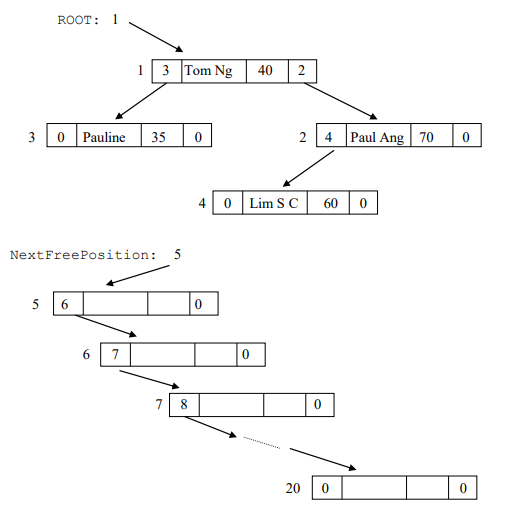
\includegraphics[width=0.5\paperwidth]{C:/Users/Admin/Desktop/Github/question_bank/LyX/static/img/9597-HCI-2017-P1-Q4-1}
\par\end{center}

The diagram shows the binary tree with the students\textquoteright{}
scores 40, 70, 35 and 60 (added in that order) and linked list of
unused nodes after the four students\textquoteright{} scores have
been added. 

\subsection*{Task 4.1 }

Write the program code to declare all the required variables and create
the initial linked list which contains all 20 nodes. Add statement(s)
to initialize the empty tree. 

\subsection*{Evidence 19 }

Your program code for Task 4.1. \hfill{}{[}8{]}

\subsection*{Task 4.2}

Write a non-recursive procedure \texttt{AddNodeToTree} to add a new
node with student\textquoteright s name and score into the binary
tree structure. 

\subsection*{Evidence 20}

Your program code for Task 4.2.\hfill{} {[}8{]}

\subsection*{Task 4.3 }

Write a procedure \texttt{OutputData} which displays the value of
\texttt{Root}, the value of \texttt{NextFreePosition} and the contents
of \texttt{ThisTree} in index order.

\subsection*{Evidence 21 }

Your program code for Task 4.3.\hfill{} {[}5{]}

\subsection*{Task 4.4 }

Write a main program to: 
\begin{itemize}
\item construct a binary search tree using the data provided in the text
file SCORES.txt by calling procedure \texttt{AddNodeToTree}. 
\item Your program will then call procedure \texttt{OutputData}. 
\end{itemize}

\subsection*{Evidence 22 }

Your program code for Task 4.4.\hfill{} {[}4{]}

\subsection*{Evidence 23 }

Screenshot showing the output from running the program in Task 4.4.\hfill{}
{[}4{]}

\subsection*{Task 4.5}

Write a recursive procedure \texttt{RankList} to output students\textquoteright{}
names and scores in descending scores order. Include a call to the
procedure from your main program. Evidence 24 Your program code for
Task 4.5.\hfill{} {[}4{]}

\subsection*{Evidence 25 }

Provide a screenshot showing students\textquoteright{} names and scores
in descending scores order. \hfill{}{[}2{]}

 \newpage 

\item \textbf{{[}PJC/PRELIM/9597/2017/P1/Q1{]} }

The text file \texttt{TEMPERATURE.txt} contains the mean daily temperature
from January 1982 to June 2017. Each line of record is in the format 
\noindent \begin{center}
\texttt{<year>-<month> <mean daily temperature> }
\par\end{center}

For examples, \texttt{1982-01 29.8} and \texttt{2017-06 31.6} 

\subsection*{Task 1.1 }

Write program code that will 
\begin{itemize}
\item read the data from the text file, 
\item calculate the average of all the available monthly temperatures by
year, by totalling up the temperatures for each month of that year
and divided by the number of months, 
\item output the average temperature for that year (from 1982 to 2017),
in 3 decimal places.
\item Use the following format: 
\noindent \begin{center}
\texttt{}%
\begin{tabular}{ccc}
\texttt{Year} &  & \texttt{Average temperature}\tabularnewline
\texttt{1982} &  & \texttt{31.442}\tabularnewline
\texttt{1983} &  & \texttt{31.750}\tabularnewline
\texttt{$\vdots$} &  & \texttt{$\vdots$}\tabularnewline
\texttt{$\vdots$} &  & \texttt{$\vdots$}\tabularnewline
\texttt{2017} &  & \texttt{31.217 }\tabularnewline
\end{tabular}\texttt{ }
\par\end{center}
\end{itemize}

\subsection*{Evidence 1: }

Program code for Task 1.1.\hfill{} {[}9{]}

\subsection*{Evidence 2: }

Screenshot of running program.\hfill{} {[}1{]}

\subsection*{Task 1.2 }

Sort by temperature and output the average temperature by year, in
ascending order of temperature. If temperatures are the same, then
display the later year before the earlier year. For example, if year
2017 and 1989 have the same temperature, then display 2017 before
1989. 

\subsection*{Evidence 3:}

Program code for Task 1.2. \hfill{}{[}7{]}

\subsection*{Evidence 4: }

Screenshot of running program. \hfill{}{[}1{]}

 \newpage 

\item \textbf{{[}PJC/PRELIM/9597/2017/P1/Q2{]} }

A circular queue is to be implemented with a fixed size array of n
elements, indexed from \texttt{0} to \texttt{(n \textendash{} 1)}.
\begin{center}
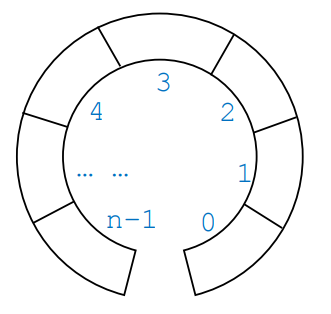
\includegraphics[width=0.2\paperwidth]{C:/Users/Admin/Desktop/Github/question_bank/LyX/static/img/9597-PJC-2017-P1-Q2-1}
\par\end{center}

\subsection*{Task 2.1 }

Following good programming practice, write program code for procedures 
\begin{itemize}
\item \texttt{setup\_queue} to set up circular queue which allows user to
input the value of \texttt{n}, 
\item \texttt{enqueue} to add an element to the queue,
\item \texttt{dequeue} to remove an element from the queue. 
\end{itemize}

\subsection*{Evidence 5: }

Program code for Task 2.1 for \texttt{setup\_queue}, \texttt{enqueue},
\texttt{dequeue}. \hfill{}{[}12{]}

\subsection*{Task 2.2 }

Write program code for a main procedure to display a menu with these
options: 
\noindent \begin{center}
\begin{tabular}{|l|}
\hline 
\texttt{1. Set up queue}\tabularnewline
\texttt{2. Add to queue}\tabularnewline
\texttt{3. Remove from queue}\tabularnewline
\texttt{4. Display queue }\tabularnewline
\texttt{5. Exit}\tabularnewline
\hline 
\end{tabular}
\par\end{center}

Write additional code to implement menu options 1, 2 and 3 using procedures
from Task 2.1. 

Also write code to implement 
\begin{itemize}
\item option 4 to display the contents of the queue and its pointers as
shown in diagram below, 
\item option 5 to exit program. 
\end{itemize}
The diagram shows the result of option 4 to display contents of queue
and pointers for \texttt{n=5} with 3 items \texttt{'fig'}, \texttt{'lemon'}
and \texttt{'cane'} in the queue:
\noindent \begin{center}
\begin{tabular}{l|l|l}
\multicolumn{1}{l}{} & \multicolumn{1}{l}{\texttt{Queue}} & \tabularnewline
 & \texttt{fig} & \texttt{<- Front pointer}\tabularnewline
 & \texttt{lemon} & \tabularnewline
 & \texttt{cane} & \texttt{<- Rear pointer}\tabularnewline
 &  & \tabularnewline
 &  & \tabularnewline
\multicolumn{1}{l}{} & \multicolumn{1}{l}{} & \tabularnewline
\multicolumn{1}{l}{} & \multicolumn{2}{l}{\texttt{Number in queue: 3}}\tabularnewline
\end{tabular}
\par\end{center}


\subsection*{Evidence 6:}

Program code for Task 2.2 for main procedure, display queue and exit
program. \hfill{}{[}8{]}

\subsection*{Task 2.3 }

Test run your program from using the following input: 
\noindent \begin{center}
\begin{tabular}{|l|}
\hline 
\texttt{Test run 1}\tabularnewline
\hline 
- \texttt{n = 8}\tabularnewline
- Add 5 words to queue in order:\tabularnewline
\texttt{'Mary', 'had', 'a', 'little', 'lamb'}\tabularnewline
- Display queue\tabularnewline
\hline 
\end{tabular}~~~~~~~~~~~%
\begin{tabular}{|l|}
\hline 
\texttt{Test run 2}\tabularnewline
\hline 
- \texttt{n = 3}\tabularnewline
- Add 4 words to queue in order:\tabularnewline
\texttt{'The', 'quick', 'brown', 'fox'}\tabularnewline
- Remove from queue\tabularnewline
- Display queue\tabularnewline
\hline 
\end{tabular}
\par\end{center}

\subsection*{Evidence 7 }

Screenshots of test runs 1 and 2. \hfill{}{[}2{]}

 \newpage 

\item \textbf{{[}PJC/PRELIM/9597/2017/P1/Q3{]} }

A linked list of nodes is used to store data for a college. The data
include name of student and exam mark. 

The linked list Abstract Data Type (ADT) has commands to create a
new linked list, add data items to the list and display the list. 

The program to implement this ADT will use the classes \texttt{Node}
and \texttt{LinkedList} as follows: 
\begin{center}
\begin{tabular}{|l|}
\hline 
\texttt{\hspace{0.25\columnwidth}Node}\tabularnewline
\hline 
\texttt{name : STRING}\tabularnewline
\texttt{mark : INTEGER}\tabularnewline
\texttt{nextPtr : INTEGER}\tabularnewline
\hline 
\texttt{constructor()}\tabularnewline
\texttt{setName(name : STRING)}\tabularnewline
\texttt{setMark(mark : INTEGER) }\tabularnewline
\texttt{setNextPtr(ptr : INTEGER)}\tabularnewline
\texttt{getName() : STRING}\tabularnewline
\texttt{getMark() : INTEGER}\tabularnewline
\texttt{getNextPtr() : INTEGER}\tabularnewline
\hline 
\end{tabular}~~~~~~%
\begin{tabular}{|l|}
\hline 
\texttt{\hspace{0.25\columnwidth}LinkedList}\tabularnewline
\hline 
\texttt{nodes : ARRAY OF Node}\tabularnewline
\texttt{head : INTEGER}\tabularnewline
\hline 
\texttt{constructor()}\tabularnewline
\texttt{addInOrder(name, mark)}\tabularnewline
\texttt{print() }\tabularnewline
\hline 
\end{tabular}
\par\end{center}

In the \texttt{Node} class, \texttt{name} and \texttt{mark} store
a student\textquoteright s name and exam mark respectively, while
\texttt{nextPtr} is a pointer to the next node. 

In the \texttt{LinkedList} class, \texttt{head} is a pointer to the
first node in the linked list. When the linked list has no data, \texttt{head}
will be set to --1.

Data added to the linked list will be stored in alphabetical order
of name. 

The print method will output for each node, in array order, the data
and pointer of each node. Page 6 

\subsection*{Task 3.1}

Write program code to define the classes \texttt{Node} and \texttt{LinkedList}.

\subsection*{Evidence 8: }

Program code for Task 3.1. \hfill{} {[}20{]}

\subsection*{Task 3.2 }

Write code to create a linked list object in the main program, read
from data file \texttt{COLLEGE.txt} and add in all the data items,
and print the array contents. The file contains name and mark of each
student in the following format:
\noindent \begin{center}
\texttt{<name>|<mark>}
\par\end{center}

Sample record: 
\noindent \begin{center}
\texttt{Jenny Tan|49}
\par\end{center}

\subsection*{Evidence 9 }

Program code for Task 3.2. Screenshot of running Task 3.2. \hfill{}
{[}5{]}

\subsection*{Task 3.3 }

Write code for a method \texttt{countNodes} to count the number of
nodes used for the data in the linked list. 

\subsection*{Evidence 10:}

Program code for Task 3.3 countNodes. \hfill{}{[}3{]}

\subsection*{Task 3.4 }

Another method \texttt{sortByMark} is to be added to the \texttt{LinkedList}
class to sort the linked list in descending order of exam mark.

Write program code to implement this method.

Test your program code by sorting the linked list from Task 3.2 in
descending order of mark. Page 7 

\subsection*{Evidence 11 }

Program code for Task 3.4 \texttt{sortByMark}.

Screenshot of running Task 3.4 \texttt{sortByMark}. \hfill{} {[}8{]}

\subsection*{Task 3.5 }

Write another method \texttt{displayByMark} to display the list of
students in descending order of mark by traversing the sorted linked
list from Task 3.4. 

\subsection*{Evidence 12 }

Program code for Task 3.5 \texttt{displayByMark}. \hfill{}{[}4{]}

 \newpage 

\item \textbf{{[}PJC/PRELIM/9597/2017/P1/Q4{]} }

Perform binary addition of positive numbers. 

\subsection*{Task 4.1 }

Write program code for a function that takes two binary numbers and
returns the result after addition of these two binary numbers.
\noindent \begin{center}
\texttt{FUNCTION addBinary(bin1, bin2: STRING) RETURN result: STRING }
\par\end{center}

\subsection*{Evidence 13 }

Program code for Task 4.1 \texttt{addBinary}. \hfill{}{[}10{]}

\subsection*{Task 4.2}

Write a main procedure that 
\begin{itemize}
\item repeatedly ask user to input binary numbers until user input \textquoteleft \texttt{XXX}\textquoteright{}
to exit program; 
\item perform validation of binary numbers; 
\item add these binary numbers using the function \texttt{addBinary}; 
\item output result of these addition. 
\end{itemize}
Sample output: 
\noindent \begin{center}
\begin{tabular}{|l|}
\hline 
\texttt{Enter binary number 1 (XXX to exit) : 1}\tabularnewline
\texttt{Enter binary number 2 (XXX to exit) : 10}\tabularnewline
\texttt{Enter binary number 3 (XXX to exit) : XXX}\tabularnewline
\texttt{Result is 11 }\tabularnewline
\hline 
\end{tabular}
\par\end{center}

\subsection*{Evidence 14 }

Program code for Task 4.2 main procedure. \hfill{} {[}8{]}

\subsection*{Evidence 15 }

Screenshot of running program with user input of the following six
binary numbers in order: \texttt{1000}, \texttt{1010}, \texttt{1100},
\texttt{0101}, \texttt{1111}, \texttt{0011}. \hfill{}{[}2{]}

These binary numbers can be found in the file \texttt{BITS.txt}.

 \newpage 

\item \textbf{{[}RVHS/PRELIM/9597/2017/P1/Q1{]} }

\textbf{Results management }

For this task, you are required to read the text file \textquotedblleft \textbf{overall\_grades.txt}\textquotedblright{}
which contains the subject grades of the first and second semester
examination of 50 students.

The format of the text file is as follow: \texttt{<name>;<subject1>:<grade1>,<grade2>;<subject2>:<grade1>,<grade
2>;<subject3>:<grade1>,<grade2>,\dots etc;\textbackslash n }

For example: 

\texttt{Rufus Schuck;EL:C,B;CL:C,C;Math:C,E;Bio:B,F; }

Student Rufus Schuck takes 4 subjects. They are English (EL), Chinese
(CL), Math (Math) and Biology (Bio). His 1st and 2nd semester grades
for English is C and B respectively. 

\subsection*{Task 1.1 }

Write the program code for the function process\_data() which reads
the text file \textquotedblleft \textbf{overall\_grades.txt}\textquotedblright{}
and returns a dictionary which has the following format. 

\texttt{\{'Rufus Schuck': \{'EL': {[}'C', 'B'{]}, 'CL': {[}'C', 'C'{]},
'Math': {[}'C', 'E'{]}, 'Bio': {[}'B', 'F'{]}\}, ...\} }

The returned dictionary uses the name of student as key and another
dictionary as its return value. This \textquotedblleft another\textquotedblright{}
dictionary then uses the subjects and a list containing the grades
of the 1st and 2nd semesters as its key and value respectively. 

\subsection*{Evidence 1 }

The program code for the function \texttt{process\_data()}. \hfill{}{[}4{]}

\subsection*{Task 1.2}

Write a function \texttt{have\_n\_improvement(n)} which takes in an
integer \texttt{n} and returns a list of student names who have improvement
in exactly \texttt{n} subject(s). Using the example in Task 1.1, '\texttt{Rufus
Schuck}' shows improvement in only English. So, if \texttt{n} is 1,
'\texttt{Rufus Schuck}' must be included in the student name list. 

\subsection*{Evidence 2}

The program code for the function \texttt{have\_n\_improvement(n)}.\hfill{}
{[}3{]}

\subsection*{Task 1.3 }

Write a function \texttt{have\_improvement\_in\_all\_subjs()} which
returns a list of student names who have improvement in all his/her
subjects. 

\subsection*{Evidence 3}

The program code for the function have\_improvement\_in\_all\_subjs(n).\hfill{}
{[}3{]}

\subsection*{Task 1.4 }

Write a function \texttt{count\_combi(combi)} which takes a list of
subjects \texttt{combi} as input and returns the total number of students
who take the subject combination in \texttt{combi}. Take note that
students who take more subjects than what is indicated in \texttt{combi}
are included. 

For example:

\noindent\begin{minipage}[t]{1\columnwidth}%
\texttt{>\textcompwordmark >\textcompwordmark > count\_combi({[}'EL',
'MATH'{]}) }

\texttt{>\textcompwordmark >\textcompwordmark > 50 }%
\end{minipage}

\subsection*{Evidence 4 }

The program code for the function \texttt{count\_combi(n)}. \hfill{}{[}4{]}

\subsection*{Task 1.5}

Using your solution in Task 1.4, find the total number of students
who take \textquotedbl Chem\textquotedbl{} and \textquotedbl Bio\textquotedbl{}
but not \textquotedbl Physics\textquotedbl . 

\subsection*{Evidence 5 }

The program code to find what is required in Task 1.5. \hfill{}{[}2{]}

\subsection*{Task 1.6 }

Write a function \texttt{calculate\_GPA(name)} which takes a string
\texttt{name} as input and calculates the GPA of the student indicated
by \texttt{name}. 

The points for each grade are as follow: 

\texttt{\{'A':5, 'B':4, 'C':3, 'D':2, 'E':1, 'F':0\} }

The 1 st and 2nd semester grades in the data has the same weightages. 

To calculate GPA,
\begin{itemize}
\item Find the average points achieved of each subject.
\begin{itemize}
\item e.g. if a student gets C and D in \textquotedbl CL\textquotedbl ,
his average points for \textquotedbl CL\textquotedbl{} is 3 + 2 =
2.5 
\end{itemize}
\item Add up the average points of each subject 
\item Divide the total by the number subjects the student takes 
\begin{itemize}
\item e.g. \texttt{'Claudette Bode': \{'EL': {[}'C', 'D'{]}, 'CL': {[}'D',
'A'{]}, 'Math': {[}'A', 'D'{]}, 'Phy': {[}'A', 'D'{]}, 'Bio': {[}'D',
'C'{]}\}}, 
\item \texttt{{[}(3 + 2)/2 + (2 + 5)/2 + (5 + 2)/2 + (2 + 5)/2 + (2 + 3)/2{]}/5
= 3.1}
\end{itemize}
\item GPA for '\texttt{Claudette Bode}' is 3.1 
\end{itemize}

\subsection*{Evidence 6 }

The program code for the function \texttt{calculate\_GPA(name)}.\hfill{}
{[}4{]}

 \newpage 

\item \textbf{{[}RVHS/PRELIM/9597/2017/P1/Q2{]} }

\textbf{Missing phone number digits }

Your friend (Mary) made an oversea friend (Jenny) yesterday while
she was studying in the regional library. To remain in contact, Jenny
gave Marry her phone number and told Mary that it is also a valid
10 digits International Standard Book Number (ISBN). 

After Jenny had left, Mary accidentally punched a few holes on the
phone number while she was arranging her notes using the library\textquoteright s
hole puncher machine. It was too difficult for Mary to recover the
lost pieces of paper. So, Mary decided to look for you to recover
the missing digits instead. Below is the picture of the paper.
\noindent \begin{center}
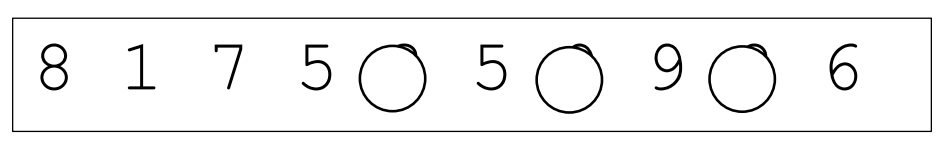
\includegraphics[width=0.5\paperwidth]{C:/Users/Admin/Desktop/Github/question_bank/LyX/static/img/9597-RHVS-2017-P1-Q1-1}
\par\end{center}

To recover the missing digits, you need to understand how ISBN-10
works. The steps to check for a valid ISBN-10 is as follow: 
\begin{enumerate}
\item[1.]  Each of the digits of the ISBN-10 is first multiplied by a number
in a sequence from 10 to 1 (Take note that the last digit of the ISBN-10
can be \textquoteleft X\textquoteright{} which holds a value of 10).
\item[2.]  All the 10 digits are then added up together. 
\item[3.]  If the sum is divisible by 11, it is a valid ISBN-10, else it is
invalid. 
\end{enumerate}
For example, to check if \textquoteleft 997150233X\textquoteright{}
is a valid ISBM-10:

\noindent %
\noindent\begin{minipage}[t]{1\columnwidth}%
\emph{Step 1 and 2}

\emph{
\begin{align*}
 & (9\times10)+(9\times9)+(7\times8)+(1\times7)+(5\times6)+(0\times5)+(2\times4)+(3\times3)+(3\times2)+(\boldsymbol{X}\times1)\\
= & (9\times10)+(9\times9)+(7\times8)+(1\times7)+(5\times6)+(0\times5)+(2\times4)+(3\times3)+(3\times2)+(\boldsymbol{10}\times1)\\
= & 297
\end{align*}
}

\emph{Step 3}

\emph{297 is a multiple of 11. Therefore, \textquoteleft 997150233X\textquoteright{}
is a valid ISBN-10. }%
\end{minipage}

\subsection*{Task 2.1}

Write a function \texttt{is\_valid\_ISBN10(isbn10)} which takes a
string \texttt{isbn10} as input and returns \texttt{True} if \texttt{isdn10}
is a valid ISBN-10 and \texttt{False} otherwise. You are to validate
the input string \texttt{isbn10} and print to terminal the issue related
to the \texttt{isbn10} string. The possible issues to be printed to
terminal includes:
\begin{itemize}
\item \texttt{ISBN-10 must only have 10 digits. }
\item \texttt{ISBN-10 can only contain numbers and the character 'X'. }
\item \texttt{'X' can only be found at the last digit of isbn10. }
\item \texttt{Wrong check digit.}
\item \texttt{Valid ISBN-10. }
\end{itemize}

\subsection*{Evidence 7 }

The program code for the function \texttt{is\_valid\_ISBN10(isbn10)}.
\hfill{}{[}6{]}

\subsection*{Task 2.2 }

Write a function \texttt{possible\_ISBN(isbn)} which takes a query
string \texttt{isbn10} as input and returns a list of possible ISBN-10.
The query string \texttt{isbn10} has 3 missing digits replaced with
a '\texttt{?}' and they can be at any positions of the query string. 

For example, 

\noindent %
\noindent\begin{minipage}[t]{1\columnwidth}%
\texttt{>\textcompwordmark >\textcompwordmark > possible\_ISBN(\textquotedbl 9971??23?X\textquotedbl ) }

\texttt{>\textcompwordmark >\textcompwordmark > {[}'997100237X',
'997102232X', '997103235X', '997104238X', '997105230X', '997106233X',
'997107236X', '997108239X', '997109231X', '997110234X', '997111237X',
'997113232X', '997114235X', '997115238X', '997116230X', '997117233X',
'997118236X', '997119239X', '997120231X', '997121234X', '997122237X',
'997124232X', '997125235X', '997126238X', '997127230X', '997128233X',
'997129236X', '997130239X', '997131231X', '997132234X', '997133237X',
'997135232X', '997136235X', '997137238X', '997138230X', '997139233X',
'997140236X', '997141239X', '997142231X', '997143234X', '997144237X',
'997146232X', '997147235X', '997148238X', '997149230X', '997150233X',
'997151236X', '997152239X', '997153231X', '997154234X', '997155237X',
'997157232X', '997158235X', '997159238X', '997160230X', '997161233X',
'997162236X', '997163239X', '997164231X', '997165234X', '997166237X',
'997168232X', '997169235X', '997170238X', '997171230X', '997172233X',
'997173236X', '997174239X', '997175231X', '997176234X', '997177237X',
'997179232X', '997180235X', '997181238X', '997182230X', '997183233X',
'997184236X', '997185239X', '997186231X', '997187234X', '997188237X',
'997190232X', '997191235X', '997192238X', '997193230X', '997194233X',
'997195236X', '997196239X', '997197231X', '997198234X', '997199237X'{]}}%
\end{minipage}

\subsection*{Evidence 8 }

The program code for the function \texttt{possible\_ISBN(isbn)}. \hfill{}{[}6{]}

\subsection*{Task 2.3}

Examine the missing numbers in the paper closely and eliminate impossible
digit choices. For example, the three missing digits cannot be \textquoteleft 1\textquoteright{}
as the three missing digits in the paper have round edges at the top.
Modify your solution in Task 2.2 and suggest these possible ISBN-10
to Mary.

\subsection*{Evidence 9 }

The screenshot of the suggested possible ISBN-10 that you will give
to Mary.\hfill{} {[}2{]}

\subsection*{Task 2.4 }

Write a menu to help other to generate possible ISBN-10. The menu
should have the following functions. 
\noindent \begin{center}
\begin{tabular}{|l|}
\hline 
\texttt{Menu}\tabularnewline
\texttt{A) Input a ISBN-10 query string}\tabularnewline
\texttt{B) Display all possible ISBN-10}\tabularnewline
\texttt{C) Quit}\tabularnewline
\hline 
\end{tabular}
\par\end{center}

You should validate user inputs and call for re-entry when an invalid
option is given. 

\subsection*{Evidence 10}

Program code for the procedure \texttt{menu()}.\hfill{} {[}6{]}

 \newpage 

\item \textbf{{[}RVHS/PRELIM/9597/2017/P1/Q3{]} }

\textbf{Unsorted Linked List}

The classes Node and LinkedList is partially implemented for you according
to the specification given below. The attribute start of class LinkedList
stores the first node instance of the linked list. If the linked list
has no node, start has the value of None. Functions in bold are not
implemented. 
\begin{center}
\texttt{}%
\begin{tabular}{|l|}
\hline 
\texttt{\hspace{0.25\columnwidth}Node}\tabularnewline
\hline 
\texttt{-data : STRING}\tabularnewline
\texttt{-next : Node}\tabularnewline
\hline 
\texttt{+constructor()}\tabularnewline
\texttt{+set\_data(data)}\tabularnewline
\texttt{+get\_data()}\tabularnewline
\texttt{+set\_next(node)}\tabularnewline
\texttt{+get\_next()}\tabularnewline
\texttt{+\_\_str\_\_()}\tabularnewline
\hline 
\end{tabular}\texttt{}%
\begin{tabular}{|l|}
\hline 
\texttt{\hspace{0.25\columnwidth}LinkedList}\tabularnewline
\hline 
\texttt{-start : Node}\tabularnewline
\tabularnewline
\hline 
\texttt{+constructor()}\tabularnewline
\texttt{+set\_start(node)}\tabularnewline
\texttt{+get\_start()}\tabularnewline
\texttt{\textbf{+insert\_data(data)}}\tabularnewline
\texttt{\textbf{+transfer(linkedlist)}}\tabularnewline
\texttt{\textbf{+delete\_pos(pos)}}\tabularnewline
\texttt{+display() }\tabularnewline
\hline 
\end{tabular}
\par\end{center}

\subsection*{Task 3}

Implement the following \texttt{LinkedList} class functions according
to its specification given: 
\begin{itemize}
\item \texttt{+insert\_data(data) : }This function takes a string \texttt{data}
as input and uses its value to create a new \texttt{Node} instance.
The new Node instance is then inserted as the first node of the linked
list\texttt{.}
\item \texttt{+transfer(llist) :} This function takes a \texttt{LinkedList}
instance \texttt{llist} as input and transfers all its \texttt{Node}
instances in the same order to the \texttt{LinkedList} instance that
calls for this function. 

For example: 

\noindent\begin{minipage}[t]{1\columnwidth}%
\texttt{A:'boy'->'man'->'woman'}

\texttt{B:'girl'->'baby' }

\texttt{>\textcompwordmark >\textcompwordmark > A.transfer(B) }

\texttt{A: 'boy'->'man'->'woman'->'girl'->'baby'}

\texttt{B: None}%
\end{minipage}
\item \texttt{+delete\_pos(pos) : }This function takes in an integer pos
as input and deletes the node at position pos. Take note that the
first node of the linked list is position 1.

For example: 

\noindent\begin{minipage}[t]{1\columnwidth}%
\texttt{A:'boy'->'man'->'woman' }

\texttt{>\textcompwordmark >\textcompwordmark > A. delete\_pos(2) }

\texttt{A:'boy'->'woman'}%
\end{minipage}
\end{itemize}

\subsection*{Evidence 11 }

Program code for: 
\begin{itemize}
\item \texttt{insert\_data(node)} \hfill{}{[}3{]}
\item \texttt{transfer(linkedlist) }\hfill{}{[}3{]}
\item \texttt{delete\_pos()}\hfill{} {[}4{]}
\end{itemize}

 \newpage 

\item \textbf{{[}RVHS/PRELIM/9597/2017/P1/Q4{]} }

\textbf{Sorting Algorithms }

The pseudocode procedure below is given a list of integers in random
order, the procedure then outputs a sorted list in ascending order. 

\noindent\fbox{\begin{minipage}[t]{1\columnwidth - 2\fboxsep - 2\fboxrule}%
\texttt{01. FUNCTION Merge\_Sort (ARRAY: arr) }

\texttt{02. \qquad{}n = SIZE(arr) }

\texttt{03. \qquad{}IF n < 2: }

\texttt{04. \qquad{}\qquad{}RETURN arr }

\texttt{05. \qquad{}END IF }

\texttt{06. \qquad{}left = Merge\_Sort(PARTITION(arr, 0, n DIV 2)) }

\texttt{07. \qquad{}right = Merge\_Sort(PARTITION(arr, n DIV 2, n)) }

\texttt{08. \qquad{}RETURN Merge(left, right) }

\texttt{09. END FUNCTION }

\texttt{10.}

\texttt{11. FUNCTION Merge (ARRAY: left, LIST: right) }

\texttt{12. \qquad{}DECLARE results: ARRAY{[}SIZE(left) + SIZE(right){]} }

\texttt{13. \qquad{}DECLARE i, j, index : INTEGER }

\texttt{14. \qquad{}i, j, index = 0, 0, 0 }

\texttt{15. \qquad{}WHILE i < SIZE(left) and j < SIZE(right)}

\texttt{16. \qquad{}\qquad{}IF left{[}i{]} < right{[}j{]}:}

\texttt{17. \qquad{}\qquad{}\qquad{}results{[}index{]} = left{[}i{]} }

\texttt{18. \qquad{}\qquad{}\qquad{}i = i + 1}

\texttt{19. \qquad{}\qquad{}ELSE: }

\texttt{20. \qquad{}\qquad{}\qquad{}results{[}index{]} = right{[}j{]}}

\texttt{21. \qquad{}\qquad{}\qquad{}j = j + 1}

\texttt{22. \qquad{}\qquad{}END IF }

\texttt{23. \qquad{}\qquad{}index = index + 1 }

\texttt{24. \qquad{}END WHILE}

\texttt{25. \qquad{}WHILE i < SIZE(left)}

\texttt{26. \qquad{}\qquad{}results{[}index{]} = left{[}i{]} }

\texttt{27. \qquad{}\qquad{}i = i + 1}

\texttt{28. \qquad{}\qquad{}index = index + 1 }

\texttt{29. \qquad{}END WHILE}

\texttt{30. \qquad{}WHILE j < SIZE(right) }

\texttt{31. \qquad{}\qquad{}results{[}index{]} = right{[}j{]} }

\texttt{32. \qquad{}\qquad{}j = j + 1 }

\texttt{33. \qquad{}\qquad{}index = index + 1 }

\texttt{34. \qquad{}END WHILE}

\texttt{35. \qquad{}RETURN results}

\texttt{36. END FUNCTION }%
\end{minipage}}

\subsection*{Task 4.1 }

Write program code to implement the given procedure. Execute the function
using the following list as the parameter. 

\texttt{{[}1, 15, 2, 4, 3, 9, 7, 10{]}} 

\subsection*{Evidence 12 }

Program Code. Screenshot showing the output. \hfill{}{[}6{]}

\subsection*{Evidence 13}

Analyze and state the time complexity of the algorithm in big $O$
notation.\hfill{} {[}1{]}

\subsection*{Task 4.2 }

Bubble sort is a common sorting algorithm, below is an implementation
of in-place bubble sort using recursion. There are three missing lines
in the pseudocode, indicated as \texttt{A}, \texttt{B} and \texttt{C}. 

\noindent\fbox{\begin{minipage}[t]{1\columnwidth - 2\fboxsep - 2\fboxrule}%
\texttt{01. PROCEDURE Bubble\_Sort (ARRAY: arr, INTEGER: n) }

\texttt{02. \qquad{}IF \_\_\_\_\_\_\_A\_\_\_\_\_\_\_:}

\texttt{03. \qquad{}\qquad{}RETURN }

\texttt{04. \qquad{}END IF }

\texttt{05. }

\texttt{06. \qquad{}FOR i FROM 0 TO (n-1): }

\texttt{07. \qquad{}\qquad{}IF \_\_\_\_\_\_\_B\_\_\_\_\_\_\_: }

\texttt{08. \qquad{}\qquad{}\qquad{}temp = arr{[}i{]} }

\texttt{09. \qquad{}\qquad{}\qquad{}arr{[}i{]} = arr{[}i+1{]} }

\texttt{10. \qquad{}\qquad{}\qquad{}arr{[}i+1{]} = temp }

\texttt{11. \qquad{}\qquad{}END IF }

\texttt{12. \qquad{}END FOR }

\texttt{13.}

\texttt{14. \qquad{}\_\_\_\_\_\_\_C\_\_\_\_\_\_\_ }

\texttt{15. END PROCEDURE }%
\end{minipage}}

Execute the procedure to sort the following list. \texttt{{[}1, 15,
2, 4, 3, 9, 7, 10{]} }

\subsection*{Evidence 14}

Complete the missing lines \texttt{A}, \texttt{B} and \texttt{C}.
\hfill{}{[}3{]}

Insert a counting mechanism to count the number of comparisons made,
and return the value as an integer. Implement the new recursive bubble
sort. 

\subsection*{Evidence 15}

Program Code. 

Screenshot showing the output of the sorted list and count value.
\hfill{}{[}4{]}

\subsection*{Evidence 16 }

Analyze and state the time complexity of the algorithm in big $O$
notation. \hfill{} {[}1{]}

\subsection*{Task 4.3}

Due to the nature of bubble sort, if no swaps are observed in a given
iteration, then there is no need for the next iteration. Implement
the improved bubble sort. Execute the function to sort the following
list.

\texttt{{[}1, 15, 2, 4, 3, 9, 7, 10{]}}

\subsection*{Evidence 17}

Program Code. Screenshot showing the output of the sorted list and
count value. \hfill{}{[}3{]}

 \newpage 

\item \textbf{{[}RVHS/PRELIM/9597/2017/P1/Q5{]} }

\textbf{Grocery Store Manager }

The grocery shop in the neighborhood ask your help to create an application
to manage the grocery store. 

First, you are tasked to work on an object-oriented solution to store
all the grocery details. The \texttt{title} of the grocery item, \texttt{cost},
\texttt{price} and \texttt{stock} of each grocery is recorded. Besides
the normal groceries, the shop identifies three unique types of grocery
too, namely:
\begin{itemize}
\item Electrical Appliance: there is a need to indicate the \texttt{power}
of the product to understand its energy consumption rate.
\item Cigarette: it is important to track the \texttt{nicotine content}
of various kinds of cigarette.
\item Alcohol: there are distinct \texttt{types} of alcohols such as wine
or beer. 
\end{itemize}
Below is an UML class diagram for your reference. 

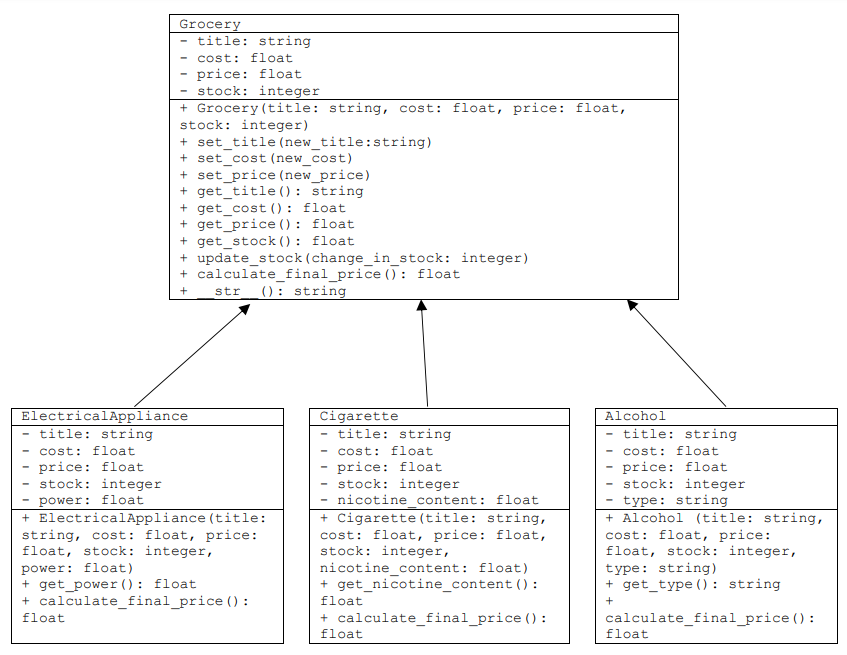
\includegraphics[width=0.65\paperwidth]{C:/Users/Admin/Desktop/Github/question_bank/LyX/static/img/9597-RVHS-2017-P1-Q5-1}

\subsection*{Task 5.1}

Implement the classes of \texttt{Grocery}, \texttt{ElectricalAppliance},
\texttt{Cigarette} and \texttt{Alcohol} with object-oriented programming.

\subsection*{Evidence 18}

Program Code for four classes. \hfill{}{[}7{]}

\subsection*{Task 5.2 }

In country S, purchasing all groceries will incur a 7\% Goods and
Services Tax(GST). 

To promote healthy living, additional tax have been imposed to cigarettes
and alcohols: 
\begin{itemize}
\item Cigarette: additional 60\% tax 
\item Wines: additional 50\% tax 
\item Beers: additional 20\% tax 
\end{itemize}
For example: \emph{the price of one packet of \textquotedblleft Yun
Yan\textquotedblright{} cigarette is \$23.00, the final price can
be calculated by: \$23.00 x 160\% x 107\% = \$39.38}

In addition, to support the \textquotedblleft save energy movement\textquotedblright ,
all electrical appliance with a power less than or equals to 10Watt
was set to be sold at 80\% of its original price. 

Implement the function \texttt{calculate\_final\_price()} which includes
the above mentioned tax and promotion into consideration. 

Implement the \texttt{\_\_str\_\_()} function which returns a string
in the following format (You may refer to the \texttt{test\_function\_5\_1()}
to understand the formatting): 

\texttt{Title | Cost | Price | Stock | Final Price }

For example, Yun Yan\textquoteright s cost is \$16.50, price is set
at \$23.00, the current stock is 4 and final price is \$39.38. The
\_\_str\_\_() function should return the following string:

\texttt{Yun Yan | \$ 16.50 | \$ 23.00 | 4 | \$ 39.38}

\subsection*{Evidence 19 }

Program Code for \texttt{calculate\_final\_price()} and \texttt{\_\_str\_\_()}. 

Screenshot showing output of \texttt{test\_function\_5\_1()}. \hfill{}{[}6{]}

\subsection*{Task 5.3}

Implement a class \texttt{StoreManager} which keep track of a list
of grocery items, \texttt{curr\_item\_list}. The \texttt{StoreManager}
should have the following class functions: 
\begin{itemize}
\item \texttt{sell\_item(sold\_item)} \texttt{sold\_item} is a tuple containing
2 elements: the \texttt{title} of the item and the \texttt{quantity}
sold. You may assume the title of item is always valid and the quantity
sold is always smaller than the current stock. 

The function should decrease the current stock of the sold items.
Upon completion, it should print out a string containing the following
information:

\texttt{Title | Unit Price | Quantity Sold | Subtotal}

The function should return a float containing the \texttt{sub\_total}
value.
\item \texttt{sell\_items(sold\_item \_list)} \texttt{sold\_item\_list}
is a list of tuples; each tuple containing the item \texttt{title}
and \texttt{quantity} sold. 

The function should print out a table displaying information for all
sold items in the following format: 

\texttt{Title | Unit Price | Quantity Sold | Subtotal}

The summary should end with a line indicating the overall total value
of items sold in this transaction. 
\item \texttt{stock\_check()} When this function is called, it should check
the list of all grocery items and print out a summary of items with
current stock value below 5. This indicates the need for stocking
up these items soon. A summary table should be printed in the following
format: 

\texttt{Title | Unit Cost | Quantity Left }
\end{itemize}

\subsection*{Evidence 20 }

Program Code for class functions of StoreManager class: 
\begin{itemize}
\item sell\_item \hfill{}{[}3{]}
\item sell\_items \hfill{}{[}2{]}
\item stock\_check \hfill{}{[}2{]}
\end{itemize}
Screenshot showing output of \texttt{test\_function\_5\_2()}.\hfill{}
{[}2{]}

 \newpage 

\item \textbf{{[}ALVL/9597/2018/P1/Q1{]} }

A program is required to input and process the number of steps taken
by members of a walking club each week. The number of steps taken
by each member is an integer in the range 0 to 100000. 

Each week, the \textquotedblleft Star of the Week\textquotedbl{} is
the member who has taken the greatest number of steps. 

The name and number of steps taken by the \textbf{previous} week's
\textquotedbl Star of the Week\textquotedbl{} are stored in the text
file, \texttt{STAR.TXT}. 

The program specification is as follows: 
\begin{itemize}
\item Input \textbf{up to} 10 names and the number of steps each has taken.
Assume that each number of steps is unique. 
\item Find the walker who has taken the greatest number of steps from this
data. 
\item Read the data about the previous \textquotedblleft Star of the Week\textquotedblright{}
from the text file \texttt{STAR. TXT}. 
\item Display a message on screen to show the previous star of the week
\textbf{and} the new star of the week, each with their number of steps.
For example, 

\texttt{Last week, Jenny Smith was 'Star of the Week' with 75827 steps
taken. }

\texttt{This week, Vanessa Lim is 'Star of the Week' with 67152 steps
taken. }
\item Update the text file, \texttt{STAR.TXT}, with the details of the new
\textquotedbl Star of the Week\textquotedblright . 
\end{itemize}

\subsubsection*{Task 1.1}

Write program code for this task that includes validation of data
entered.

\subsubsection*{Evidence 1}

Your program code. \hfill{}{[}8{]}

The program needs to be tested with different test cases. Consider
carefully, test cases for input of names and steps. 

\subsubsection*{Task 1.2}

Copy the table with the following headings. Add other test cases to
the table. One type of test case has already been added to the table.
\begin{center}
\begin{tabular}{|l|l|l|}
\hline 
\hspace{0.05\columnwidth}\textbf{Test case} & \textbf{Purpose of test data} & \textbf{Expected results}\tabularnewline
\hline 
Yi Ling Aw, 10232 & Test the maximum of 10 values & 10 values entered and star of\tabularnewline
Ryan Batisah, 42231 & entered into the program. & the week is Vanessa Lim with\tabularnewline
Lee Casmir, 35020 &  & 67152 steps taken.\tabularnewline
Daniel Bennett, 60192 &  & \tabularnewline
Sarah Heng Chee, 29389 &  & \tabularnewline
Vanessa Lim, 67152 &  & \tabularnewline
Wong Yip, 53231 &  & \tabularnewline
Rin Xie, 34200 &  & \tabularnewline
Tin Wee, 49480 &  & \tabularnewline
David Bala, 32010 &  & \tabularnewline
\hline 
\end{tabular}
\par\end{center}

\subsubsection*{Evidence 2}

Completed table with other test cases added. \hfill{}{[}4{]}

\subsubsection*{Task 1.3}

Use \textbf{three} of the test cases in the table, and produce a screenshot
for each.

\subsubsection*{Evidence 2}

Three screenshots of test cases.\hfill{}{[}3{]}

 \newpage 

\item \textbf{{[}ALVL/9597/2018/P1/Q2{]} }

The following algorithm is an implementation of a quick sort that
operates on an array \texttt{Scores}. 

This algorithm assumes that the first element of an array is the zeroth
element. This means that \texttt{Scores{[}0{]}} is the first element
in the array.

This pseudocode is available in the file \texttt{QUICKSORT.TXT}

\noindent\begin{minipage}[t]{1\columnwidth}%
\noindent \texttt{FUNCTION QuickSort(Scores)}

\noindent \texttt{\qquad{}QuickSortHelper(Scores, 0, LENGTH(Scores)
- 1)}

\noindent \texttt{\qquad{}RETURN Scores}

\noindent \texttt{ENDFUNCTION}

\bigskip{}

\noindent \texttt{FUNCTION QuickSortHelper(Scores, First, Last)}

\noindent \texttt{\qquad{}IF First < Last}

\noindent \texttt{\qquad{}THEN}

\noindent \texttt{\qquad{}\qquad{}SplitPoint <- PartitioniScores,
First, Last)}

\noindent \texttt{\qquad{}\qquad{}QuickSortHelper(Scores, First,
SplitPoint \textemdash{} 1)}

\noindent \texttt{\qquad{}\qquad{}QuickSoRtHelper(Scores, SplitPoint
+ 1, Last)}

\noindent \texttt{\qquad{}ENDIF}

\noindent \texttt{\qquad{}RETURN Scores}

\noindent \texttt{ENDFUNCTION }\bigskip{}

\noindent \texttt{FUNCTION Partition(Scores, First, Last)}

\noindent \texttt{\qquad{}PivotValue <- ScoresiFirst{]}}

\noindent \texttt{\qquad{}Lefthark <- First + 1}

\noindent \texttt{\qquad{}RightMark <- Last}

\noindent \texttt{\qquad{}Done <- FALSE}

\noindent \texttt{\qquad{}WHILE (Done = FALSE)}

\noindent \texttt{\qquad{}\qquad{}WHILE LeftMark <= RightMark AND
Scores{[}LeftMark{]} <= PivotValue}

\noindent \texttt{\qquad{}\qquad{}\qquad{}LeftMark <- LeftMark
+ 1}

\noindent \texttt{\qquad{}\qquad{}ENDWHILE}

\noindent \texttt{\qquad{}\qquad{}WHILE Scores{[}RightMark{]} >=
PivotValue AND RightMark >= LeftMark}

\noindent \texttt{\qquad{}\qquad{}\qquad{}RightMark <- RightMark
\textemdash{} 1}

\noindent \texttt{\qquad{}\qquad{}ENDWHILE}

\noindent \texttt{\qquad{}\qquad{}IF RightMark < LeftMark}

\noindent \texttt{\qquad{}\qquad{}\qquad{}THEN}

\noindent \texttt{\qquad{}\qquad{}\qquad{}\qquad{}Done <- TRUE}

\noindent \texttt{\qquad{}\qquad{}ELSE}

\noindent \texttt{\qquad{}\qquad{}\qquad{}Temp <- Scores{[}LeftMark{]}}

\noindent \texttt{\qquad{}\qquad{}\qquad{}Scores{[}LeftMark{]}
<- Scores{[}RightMark{]}}

\noindent \texttt{\qquad{}\qquad{}\qquad{}Scores{[}RightMark{]}
<- Temp}

\noindent \texttt{\qquad{}ENDIF}

\noindent \texttt{ENDWHILE }\bigskip{}

\noindent \texttt{\textbf{\emph{<swap Scores{[}First{]} with Scores{[}RightMark{]}>}}}\texttt{
}\bigskip{}

\noindent \texttt{\qquad{}RETURN RightMark}

\noindent \texttt{ENDFUNCTION}%
\end{minipage}

\subsubsection*{Task 2.1}

Write program code to implement this algorithm. Ensure that you add
the missing code to complete the algorithm. The area of missing code
is highlighted as:
\begin{center}
\texttt{\textbf{\emph{<swap Scores {[}First{]} with Scores {[}RightMark{]}>}}}
\par\end{center}

Copy the sample data available in the \texttt{SCORES.TXT} file. Paste
this into your programming code to set up the data to be sorted.

\subsubsection*{Evidence 4}

Your program code. \hfill{}{[}12{]}

\subsubsection*{Task 2.2}

Add a function to your code to output Scores. Call this function before
and after the operation of the quick sort so that the unsorted and
sorted data is displayed.

\subsubsection*{Evidence 5}

Your program code. \hfill{}{[}2{]}

\subsubsection*{Evidence 6}

Screenshot showing the unsorted and sorted \texttt{Scores} data.\hfill{}
{[}1{]}

 \newpage 

\item \textbf{{[}ALVL/9597/2018/P1/Q3{]} }

The file,\texttt{ HASHEDDATA.TXT}, holds details of the names and
telephone numbers of 250 people. 

There are a total of 500 lines in the file, and a number of these
lines are empty of name and telephone number.

An index is stored for each line of the file. 

The format of the data in the file is: 
\begin{center}
<Index>,<PersonName>,<TelephoneNumber> 
\par\end{center}

The first 10 lines from the file are shown as follows: 

\noindent\fbox{\begin{minipage}[t]{1\columnwidth - 2\fboxsep - 2\fboxrule}%
0, ,

1, ,

2, ,

3, Boon Keng V., 07492 546415

4, ,

5, ,

6, Ahmad Yusof, 07439 778665

7, Durno Peter, 07662 863518

8, Batisah Wong, 07362 156265

9, ,%
\end{minipage}}

The values in the file are separated by the comma character. 

A record structure is used to store a name and telephone number. A
data structure of 500 records is needed to store all the names and
telephone numbers. Each line in the file is written to a corresponding
position in the data structure.

The records with index six to eight from the data structure are: 
\begin{center}
\begin{tabular}{r|c|c|}
\cline{2-3} \cline{3-3} 
\textbf{Index} & \textbf{PersonName} & \textbf{TelephoneNumber}\tabularnewline
\cline{2-3} \cline{3-3} 
6 & Ahmad Yusof & 07439 778665\tabularnewline
\cline{2-3} \cline{3-3} 
7 & Durno Peter & 07662 863518\tabularnewline
\cline{2-3} \cline{3-3} 
\texttt{8} & Batisah Wong & 07362 156265\tabularnewline
\cline{2-3} \cline{3-3} 
\end{tabular}
\par\end{center}

\subsubsection*{Task 3.1}

Use program code to create a:
\begin{itemize}
\item record structure to hold the name and telephone number for one person
\item data structure, using this record structure to store 500 records.
\end{itemize}

\subsubsection*{Evidence 7}

Your program code. \hfill{}{[}6{]}

\subsubsection*{Task 3.2}

Write program code to:
\begin{itemize}
\item read the lines from the file
\item extract the <Index>, <PersonName> and <TelephoneNumber> values
\item store these values in the data structure.
\end{itemize}
Create a procedure called \texttt{DisplayValues} that will loop though
the data structure and display the index, name and telephone number
for every record where the name is present.

Ensure your procedure uses headings to identify the data displayed.

\subsubsection*{Evidence 8}

Your program code. \hfill{}{[}13{]}

\subsubsection*{Evidence 9}

A Screenshot showing the output.\hfill{} {[}1{]}

A hashing function was used to create the file. The same hashing function
can be used to search the data structure for a particular name. The
hashing function generates a hash. This is calculated as follows:

\noindent\begin{minipage}[t]{1\columnwidth}%
\texttt{Get SearchName}

\texttt{Set HashTotal to 0}

\texttt{FOR each Character in SearchName}

\texttt{\qquad{}Get the ASCII code for Character}

\texttt{\qquad{}Multiply the ASCII code by the position of Character
in SearchName}

\texttt{\qquad{}Add the result to the HashTotal}

\texttt{Calculate Hash as HashTotal MOD 500}

\texttt{RETURN Hash}%
\end{minipage}

\subsubsection*{Task 3.3}

Add the program code for the hashing function. Use the following specification:
\begin{center}
\texttt{FUNCTION GenerateHash(SearchName : STRING) : INTEGER}
\par\end{center}

The function has a single parameter \texttt{SearchName} and returns
an integer value.

Write additional code for your program to allow you to test the implementation
of this function.

The following test data will assist you.

\qquad{}\textquotedblleft Tait Davinder\textquotedblright{} should
return a hash of 87

\qquad{}\textquotedblleft Anandan Yeo\textquotedbl{} should return
a hash of 156

\subsubsection*{Evidence 10}

Your program code. \hfill{}{[}8{]}

\subsubsection*{Evidence 11}

A screenshot (or screenshots) of your program to show the results
of the hash calculation for both the given test data values.\hfill{}{[}2{]}

The hash calculated from the \texttt{SearchName} can be used to find
a corresponding record in the data structure.

If the \texttt{SearchName} is not found in the record given by the
hash \textbf{and} the record is not empty:
\begin{itemize}
\item compare \texttt{SearchName} with the next record
\item until the \texttt{SearchName} is found or an empty record is found.
\end{itemize}
If an empty record is found then the program will report that the
name is \textquotedblleft NOT FOUND\textquotedblright .

If the record is found, the program will output the index, name and
telephone number.

\subsubsection*{Task 3.4}

Add the program code to implement the search as described.

\subsubsection*{Evidence 12}

Your program code. \hfill{}{[}7{]}

\subsubsection*{Evidence 11}

A screenshot (or screenshots) of your program to show the results
of the following searches:

Search 1: Charlie Love

Search 2: Chin Tan

Search 3: John Barrowman\hfill{}{[}3{]}

 \newpage 

\item \textbf{{[}ALVL/9597/2018/P1/Q4{]} }

In a computer game, a player (\textquotedbl\texttt{O}\textquotedbl )
moves around a maze measuring 10 metres by 11 metres to collect a
prize (\textquotedbl\texttt{P}\textquotedbl ). The prize is placed
at a random position within the maze. The prize position is not where
a wall (\textquotedbl\texttt{X}\textquotedbl ) appears in the maze.
An empty position is indicated with a full-stop (\textquotedbl\texttt{.}\textquotedbl ). 

The maze is represented on the screen by a rectangular grid. Each
square metre of the maze is represented by an x-coordinate and a y-coordinate.
The top left square metre of the puzzle display has x = \texttt{0}
and y = \texttt{0}.

The player moves left, right, up or down according to a direction
entered by the user. The game is turn-based; a user enters the direction,
their player moves one position in that direction. lithe direction
would place the player on a well, then the player does not move. The
maze is displayed after each move.
\begin{center}
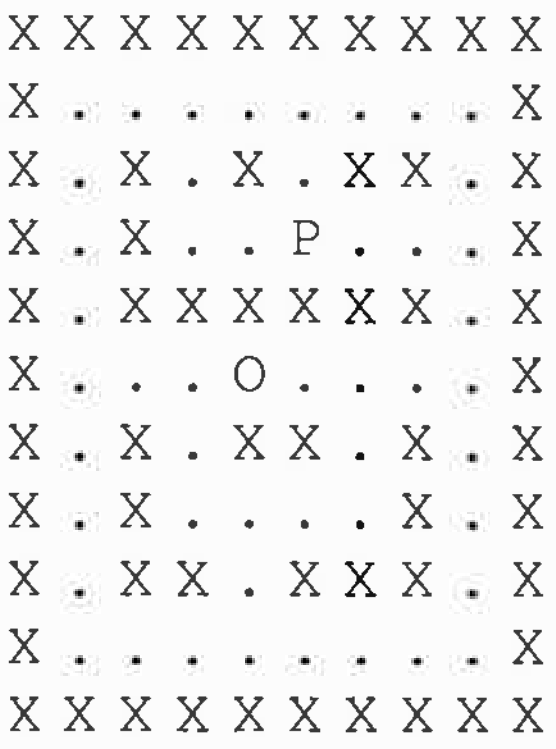
\includegraphics[width=0.25\paperwidth]{C:/Users/Admin/Desktop/Github/question_bank/LyX/static/img/9597-ALVL-2018-P1-Q4}
\par\end{center}

\subsubsection*{Task 4.1}

Write a program to display the maze as shown.
\begin{itemize}
\item The maze should be stored in a suitable data structure.
\item The data structure will allow fixed loop(s) to be used to display
the maze.
\end{itemize}
The maze is given in the text file \texttt{MAZE.TXT}. You may read
in the data from this file or place the data in your program using
any suitable method.

\subsubsection*{Evidence 14}

Your program code. \hfill{} {[}6{]}

\subsubsection*{Task 4.2}

The prize is placed randomly on the maze. It cannot appear in the
same grid position as a wall (\textquotedbl\texttt{X}\textquotedbl ).

Add to your program code to place the prize at a random position.

Take a screenshot of the maze with the prize displayed in it.

\subsubsection*{Evidence 15}

Your program code. \hfill{}{[}4{]}

\subsubsection*{Evidence 16}

A screenshot of the maze as output by your program. \hfill{} {[}1{]}

The player is represented by the character \textquotedbl\texttt{O}\textquotedbl .
The character starts the game in a central position on the grid, for
example, x = \texttt{4} and y = \texttt{5}. 

To move the character, the user is prompted for a direction. The following
are valid inputs:
\begin{center}
\begin{tabular}{|c|l|}
\hline 
\textbf{Input character} & \hspace{0.05\columnwidth}\textbf{Action}\tabularnewline
\hline 
\texttt{``U''} & Player moves up\tabularnewline
\hline 
\texttt{``D''} & Player moves down\tabularnewline
\hline 
\texttt{``L''} & Player moves left\tabularnewline
\hline 
\texttt{``R''} & Player moves right\tabularnewline
\hline 
\texttt{``''} & Continue with previous move.\tabularnewline
 & If no previous move, do nothing\tabularnewline
\hline 
\end{tabular}
\par\end{center}

If the next position for the player (\textquotedbl\texttt{O}\textquotedbl )
is a wall (\textquotedbl\texttt{X}\textquotedbl ), then the player
stays in their current position; this is called collision detection.

When the player enters the move, a new position for the player (\textquotedbl\texttt{O}\textquotedbl )
is calculated and the maze is displayed. The previous position is
changed back to a \textquotedbl .\textquotedbl{} when the player
has a new position. The moves are repeated until the player is at
the same position as the prize.

\subsubsection*{Task 4.3}

Add to your program code to:
\begin{itemize}
\item place the player on the grid at a central position on the grid
\item take in and validate a direction
\item calculate a new position
\item check this position is not a wall
\item update the grid so that the previous position of \textquotedbl\texttt{O}\textquotedbl{}
is replaced with a \textquotedbl{} . \textquotedbl{} and \textquotedbl\texttt{O}\textquotedbl{}
is located in its new position
\item continue this until the player is at the same position as the prize.
\end{itemize}

\subsubsection*{Evidence 17}

Your program code. \hfill{} {[}16{]}

When the player and the prize are at the same position, the message
\textquotedblleft Player has reached the prize\textquotedblright{}
is displayed and the game ends.

\subsubsection*{Task 4.4}

Add to your program, code to end the game when this condition is met,
and display the required message. Produce screenshots to show key
elements of your program are functioning.

The screenshots required are:
\begin{itemize}
\item entering each direction
\item player changing position
\item end of game
\end{itemize}

\subsubsection*{Evidence 18}

Your program code. \hfill{} {[}1{]}

\subsubsection*{Evidence 19}

Screenshots of:
\begin{itemize}
\item entering each direction
\item player changing position
\item end of game (player wins) \hfill{} {[}2{]}
\end{itemize}

 \newpage 

\item \textbf{{[}ALVL/9597/2018/P2/Q1{]} }

A mobile phone company has an option for Pay As You Go usage. Customers
have to purchase credit in advance. The credit is used to pay for
texts, calls and data. Customers can buy additional credit at any
time. 

The company requires software to allow their Pay As You Go customers
to do the following tasks online: 
\begin{itemize}
\item check credit balance 
\item check data usage 
\item check call usage 
\item pay for credit 
\end{itemize}
A software company was employed to put together a project team to
produce the software. 
\begin{enumerate}
\item State \textbf{three} members of the project team. Describe the role
of each of these members. \hfill{}{[}6{]}
\item The initial phase of the system development cycle required that a
specification be created for the system. 
\begin{enumerate}
\item State \textbf{two} techniques that could have been used to gather
the information for this specification. \hfill{} {[}2{]}
\item Explain how each technique would have been used in this project. \hfill{}
{[}4{]}
\end{enumerate}
\item The specification is a detailed report.

Describe \textbf{two} sections of this report. \hfill{}{[}4{]}
\item The software could have been designed using different techniques. 
\begin{enumerate}
\item Name \textbf{and} describe \textbf{two} design techniques that may
have been used. \hfill{} {[}4{]}
\item Explain why it is important for each member of the design team to
use the same technique. \hfill{} {[}2{]}
\item A customer's mobile phone number needs to be validated on entry. 

Draw a flowchart to represent an algorithm for this validation. \hfill{}
{[}4{]}
\end{enumerate}
\item (e) The work to implement the new software needs to be managed. The
following Program Evaluation and Review Technique (PERT) chart is
used as a management tool. 

\texttt{A} --- Specification 

\texttt{B} --- Analysis 

\texttt{C} --- Design of software 

\texttt{D} --- Design of Interface 

\texttt{E} --- Documentation 

\texttt{F}--- Implementation 

\texttt{G} --- Testing 

\texttt{H} --- Acceptance testing

\texttt{I} --- Hand over to phone company 

Time is measured in weeks. 
\begin{center}
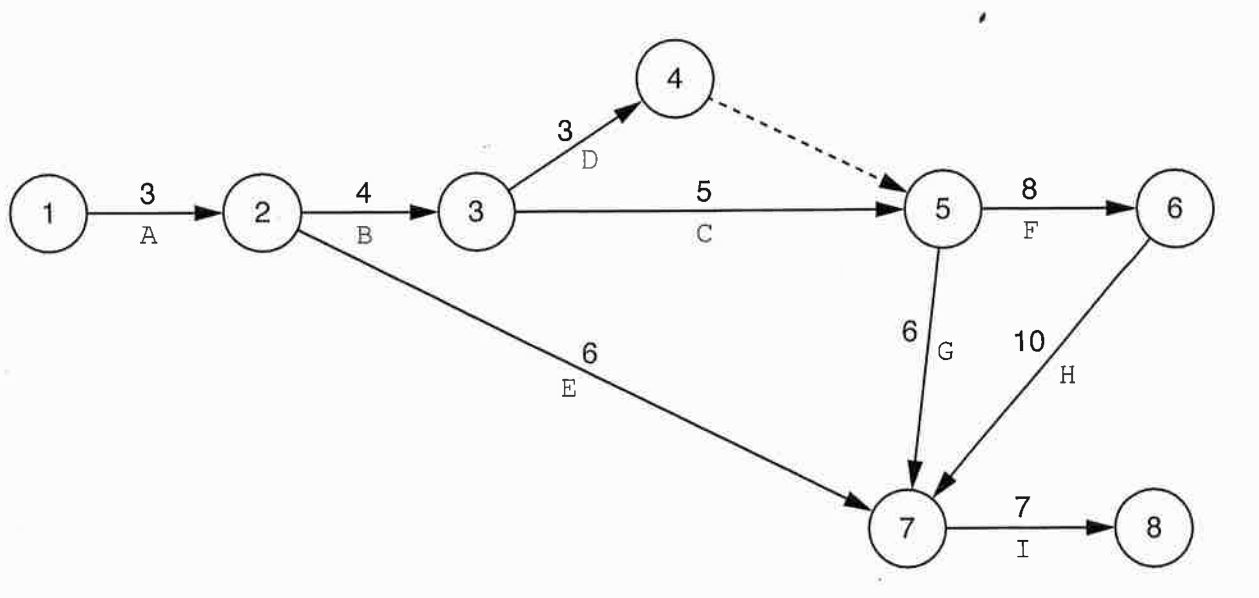
\includegraphics[width=0.5\paperwidth]{C:/Users/Admin/Desktop/Github/question_bank/LyX/static/img/9597-ALVL-2018-P2-Q1}
\par\end{center}
\begin{enumerate}
\item State the critical path for the given activities \texttt{A} to \texttt{I}.
\hfill{}{[}2{]}
\item Calculate the minimum time these activities will take. \hfill{}{[}1{]}
\item The member of the project team who worked on activity 0 fold the project
manager he could not start work until one week after the scheduled
start date. 

Explain any impact this would have on the completion date of the project.\hfill{}
{[}3{]}
\end{enumerate}
\item The software is intended for use on hand-held devices. 

Describe \textbf{two} ways that users can keep their data secure on
these devices.\hfill{} {[}4{]}
\item A member of the project team had the task of ensuring that social
and ethical issues were considered. 

Describe \textbf{one} example of each of these Issues that this member
of the team might have considered. \hfill{}{[}4{]}
\end{enumerate}

 \newpage 

\item \textbf{{[}ALVL/9597/2018/P2/Q2{]} }

The following algorithm calculates the average mark for a group of
students. 

\noindent\begin{minipage}[t]{1\columnwidth}%
\texttt{01 FOR Counter <- 1 TO NumberOfStudents}

\texttt{02 \qquad{}Total <- O}

\texttt{03 \qquad{}INPUT Mark}

\texttt{04 \qquad{}Total <- Total + Mark}

\texttt{05 ENDFOR}

\texttt{06 Average <- Total / NumberOfStudents}

\texttt{07 OUTPUT Average}%
\end{minipage}
\begin{enumerate}
\item There is an error in this algorithm causing an incorrect result. Describe
the error and explain the change required to correct this error. \hfill{}{[}3{]}
\item State the name of this type of error.\hfill{} {[}1{]}
\item The lowest mark in the exam is 0 and the highest is 100. Give an example
from each of the appropriate test cases which could be used to test
the algorithm. \hfill{}{[}4{]}
\item Name and describe a suitable technique that could be used to manually
identify errors in the algorithm. \hfill{}{[}2{]}
\end{enumerate}

 \newpage 

\item \textbf{{[}ALVL/9597/2018/P2/Q3{]} }
\begin{enumerate}
\item A binary tree is as follows: 
\begin{center}
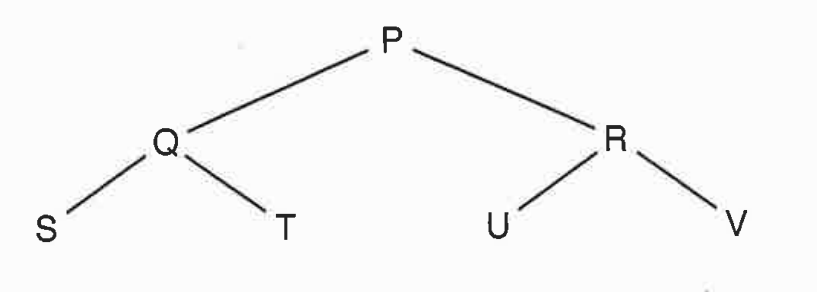
\includegraphics[width=0.5\paperwidth]{C:/Users/Admin/Desktop/Github/question_bank/LyX/static/img/9597-ALVL-2018-P2-Q3}
\par\end{center}
\begin{enumerate}
\item State the in-order sequence. \hfill{}{[}1{]}
\item State the pre-order sequence. \hfill{} {[}1{]}
\end{enumerate}
\item A 1D array, \texttt{Value}, stores a list of scores as follows:
\begin{center}
\begin{tabular}{|c|c|c|c|c|c|c|c|c|c|c|c|c|c|c|c|}
\hline 
Index & 0 & 1 & 2 & 3 & 4 & 5 & 6 & 7 & 8 & 9 & 10 & 11 & 12 & 13 & 14\tabularnewline
\hline 
Score & 2 & 6 & 15 & 23 & 36 & 48 & 50 & 58 & 64 & 69 & 74 & 79 & 86 & 92 & 99\tabularnewline
\hline 
\end{tabular}
\par\end{center}
\begin{enumerate}
\item Using a linear search, state how many comparisons will be required
to find the score of 64. \hfill{}{[}1{]}
\end{enumerate}
The following binary search algorithm could be used to search the
list of scores.

\noindent\begin{minipage}[t]{1\columnwidth}%
\texttt{01 Lower <- LowestIndex}

\texttt{02 Upper <- HighestIndex}

\texttt{03 REPEAT}

\texttt{04 \qquad{}Middle <- (Lower + Upper) DIV 2}

\texttt{05 \qquad{}IF SearchItem > Value{[}Middle{]}}

\texttt{O6 \qquad{}THEN}

\texttt{07 \qquad{}\qquad{}Lower <- Middle + l}

\texttt{08 \qquad{}ELSE}

\texttt{09 \qquad{}\qquad{}Upper <- Middle \textemdash{} l}

\texttt{10 \qquad{}ENDIF}

\texttt{11 UNTIL Value{[}Middle{]} = SearchItem OR Lower > Upper}

\texttt{12 OUTPUT \textquotedbl Score found at position\textquotedbl{}
Middle}%
\end{minipage}
\begin{enumerate}
\item[ii.] Score 80 is not in the list.

When searching for this score, state the values that will be examined.
\hfill{}{[}2{]}
\item[iii.] When searching for a score of 80, this algorithm outputs:

\texttt{Score found at position 12}

Describe how the algorithm gives this incorrect output. \hfill{}{[}2{]}
\item[iv.] Describe how the algorithm could be changed to give a suitable message
if the score is not in the list. \hfill{}{[}3{]}
\end{enumerate}
\end{enumerate}

 \newpage 

\item \textbf{{[}ALVL/9597/2018/P2/Q4{]} }

A university allows students to access the university network from
home. 
\begin{enumerate}
\item The university server has a firewall.

Describe \textbf{two} ways that a firewall can be used to block unauthorised
access to the network. \hfill{}{[}2{]}
\item The university wishes to restrict access to inappropriate websites
from within its network.

Describe \textbf{two} methods that could be used to restrict access
to inappropriate websites. \hfill{}{[}4{]}
\item The university is concerned about the possible loss of data from their
local servers.

Describe a strategy that could be used to prevent data loss. \hfill{}{[}2{]}
\item The university has its own intranet.

Describe \textbf{two} benefits that the intranet might provide for
students. \hfill{}{[}2{]}
\end{enumerate}

 \newpage 

\item \textbf{{[}ALVL/9597/2018/P2/Q5{]} }

The organisers of a diving championship have created software to calculate
and show the total score for each diver. 

There are nine judges scoring each dive. The two best scores and the
two worst scores are ignored. The other five scores are added together
to give the diver\textquoteright s total score. 
\begin{enumerate}
\item Write an algorithm to take in the nine scores, delete the best two
and the two worst scores, and total the five remaining scores. \hfill{}{[}4{]}
\end{enumerate}
There are 10 divers in the final. The scoreboard shows the order of
diving. 
\begin{center}
\begin{tabular}{|c|c|l|}
\hline 
\textbf{Order} & \textbf{Diver name} & \textbf{Total score}\tabularnewline
\hline 
1 & Daniel Tan & \tabularnewline
\hline 
2 & Parker Lam & \tabularnewline
\hline 
3 & Mohamed Noor & \tabularnewline
\hline 
4 & Hariz Yazid & \tabularnewline
\hline 
5 & Sheryl Xuan & \tabularnewline
\hline 
6 & Karl Lim & \tabularnewline
\hline 
7 & Elaine Ning & \tabularnewline
\hline 
8 & Nadyia Esmadi & \tabularnewline
\hline 
9 & Cai Ng & \tabularnewline
\hline 
10 & Hamid Mahmood & \tabularnewline
\hline 
\end{tabular}
\par\end{center}
\begin{enumerate}
\item The programmers decided to use a 1D array for the scores. They will
also use a bubble sort to sort the scores into descending order.
\begin{enumerate}
\item Explain how a bubble sort can be used to arrange the scores into a
descending or ascending order. \hfill{}{[}2{]}
\end{enumerate}
This is the bubble sort algorithm for sorting into descending order:

\noindent\begin{minipage}[t]{1\columnwidth}%
\texttt{01 WHILE NoSwaps = FALSE}

\texttt{02 \qquad{}NoSwaps <- TRUE}

\texttt{03 \qquad{}UpperBound <- ListLength}

\texttt{04 \qquad{}FOR Posn <- 0 TO ......}\texttt{\textbf{A}}\texttt{......}

\texttt{05 \qquad{}\qquad{}IF List{[}Posn{]} < ......}\texttt{\textbf{B}}\texttt{......}

\texttt{06 \qquad{}\qquad{}\qquad{}THEN}

\texttt{O7 \qquad{}\qquad{}\qquad{}\qquad{}// Swap}

\texttt{O8 \qquad{}\qquad{}\qquad{}\qquad{}NoSwaps <- ......}\texttt{\textbf{C}}\texttt{......}

\texttt{09 \qquad{}\qquad{}\qquad{}\qquad{}Temp <- List{[}Posn{]}}

\texttt{10 \qquad{}\qquad{}\qquad{}\qquad{}List{[}Posn{]} <- ListiPosn
+ 1{]}}

\texttt{11 \qquad{}\qquad{}\qquad{}\qquad{}List{[}Posn + 1{]}
<- ......}\texttt{\textbf{D}}\texttt{......}

\texttt{12 \qquad{}\qquad{}ENDIF}

\texttt{l3 \qquad{}ENDFOR}

\texttt{14 ENDWHILE}%
\end{minipage}
\begin{enumerate}
\item Write the pseudocode for \texttt{\textbf{A}}, \texttt{\textbf{B}},
\texttt{\textbf{C}}\textbf{ a}nd \texttt{\textbf{D}} in the algorithm.
\hfill{} {[}4{]}
\end{enumerate}
\item During the first round of dives, the sorted scores for five divers
are: 

\texttt{48 }

\texttt{45 }

\texttt{40 }

\texttt{37 }

\texttt{36 }

The sixth diver scores 42 and the software appends the score to the
list as follows: 

\texttt{48 }

\texttt{45 }

\texttt{40 }

\texttt{37 }

\texttt{36 }

\texttt{42}
\begin{enumerate}
\item State the number of passes needed through the list to return the list
to its sorted order. \hfill{}{[}1{]}
\item Explain why the bubble sort is efficient in this example. \hfill{}{[}2{]}
\item Name another sort method that could have been used in this situation. 

Compare the speed of sorting the divers\textquoteright{} scores in
your named method with using the bubble sort. \hfill{}{[}2{]}
\end{enumerate}
\end{enumerate}

 \newpage 

\item \textbf{{[}ALVL/9597/2018/P2/Q6{]} }

Customers want to buy tickets for a diving championship that takes
place over three days. There are two sessions of diving each day. 

Customers use a ticket ordering website to buy their tickets.
\begin{center}
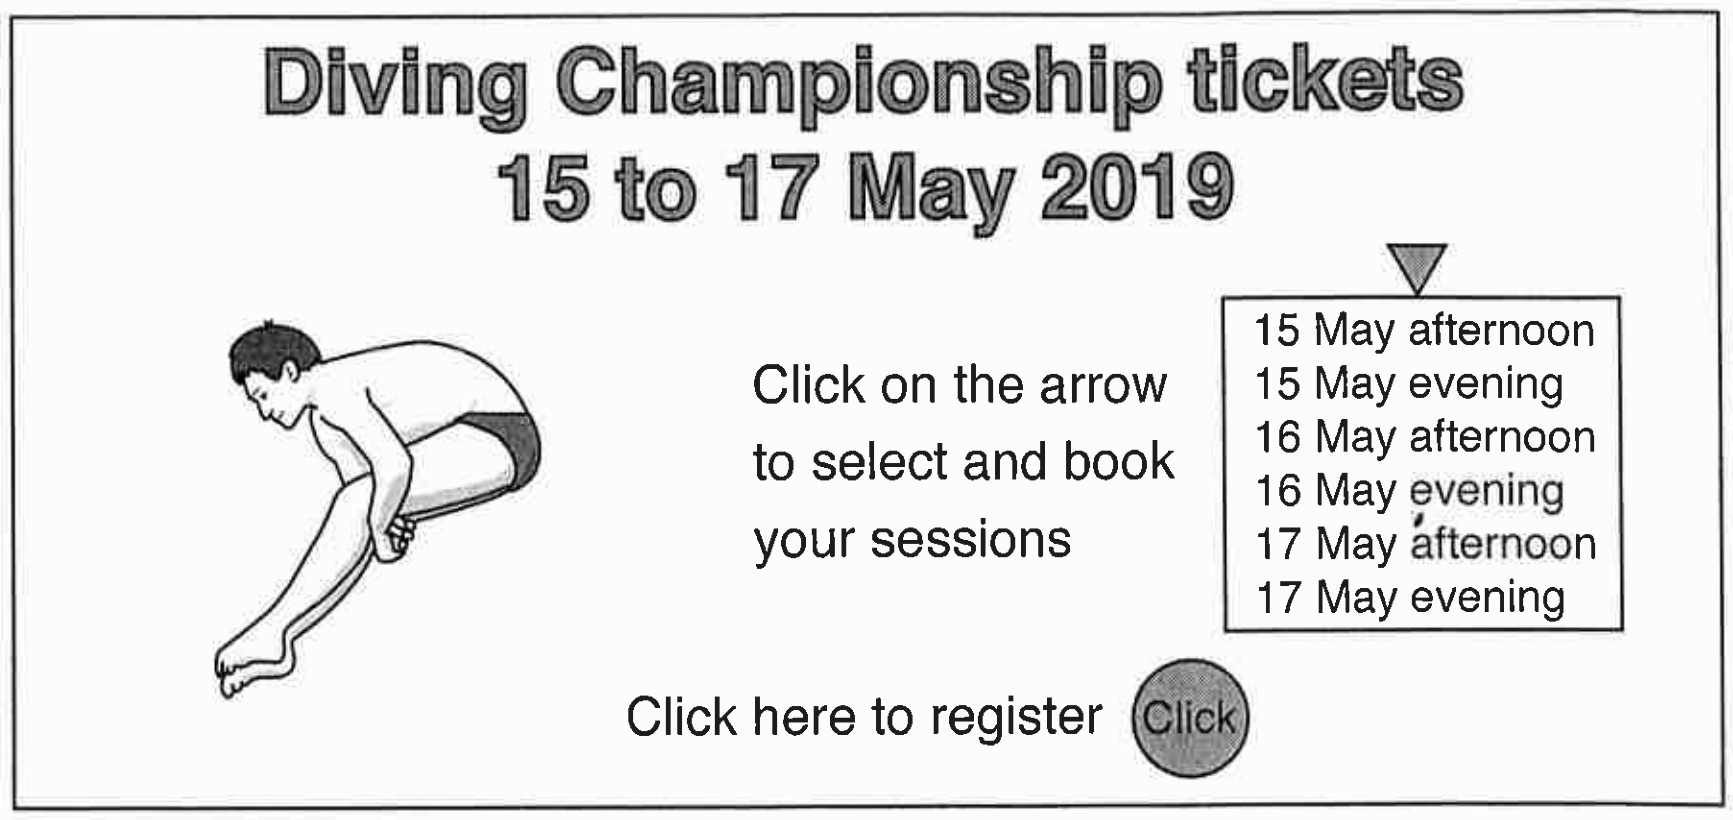
\includegraphics[width=0.5\paperwidth]{C:/Users/Admin/Desktop/Github/question_bank/LyX/static/img/9597-ALVL-2018-P2-Q6-1}
\par\end{center}
\begin{enumerate}
\item State the type of user interface that the ticket ordering website
uses. \hfill{}{[}1{]}
\item All ticket sales are stored on a database server in the following
tables: 

\texttt{CUSTOMER(}\texttt{\uline{CustomerID}}\texttt{, CustomerName,
Email, ContactNumber) }

\texttt{BOOKING(}\texttt{\uline{BookinoID}}\texttt{, BookingDate,
CustomerID) }

\texttt{SESSION(}\texttt{\uline{SessionID}}\texttt{, Date, Time,
SessionCost) }

\texttt{BOOKING\_SESSION(}\texttt{\uline{BookingID}}\texttt{, }\texttt{\uline{SessionID}}\texttt{,
Quantity)} 

\texttt{CustomerID} is the unique identifier in the \texttt{CUSTOMER}
table. 

\texttt{BookingID} is the unique identifier in the \texttt{BOOKING}
table. 

\texttt{SessionID} is the unique identifier in the \texttt{SESSION}
table. 
\begin{enumerate}
\item Draw an Entity-Relationship (E-R) diagram to represent this data model.
\hfill{}{[}4{]}
\item Name the fields that would be used to calculate the customer\textquoteright s
payment for a session. \hfill{}{[}2{]}
\end{enumerate}
\item Before customers can make an online ticket purchase, they have to
fill in a registration form. The details from this form are used to
complete the CUSTOMER table. 
\begin{center}
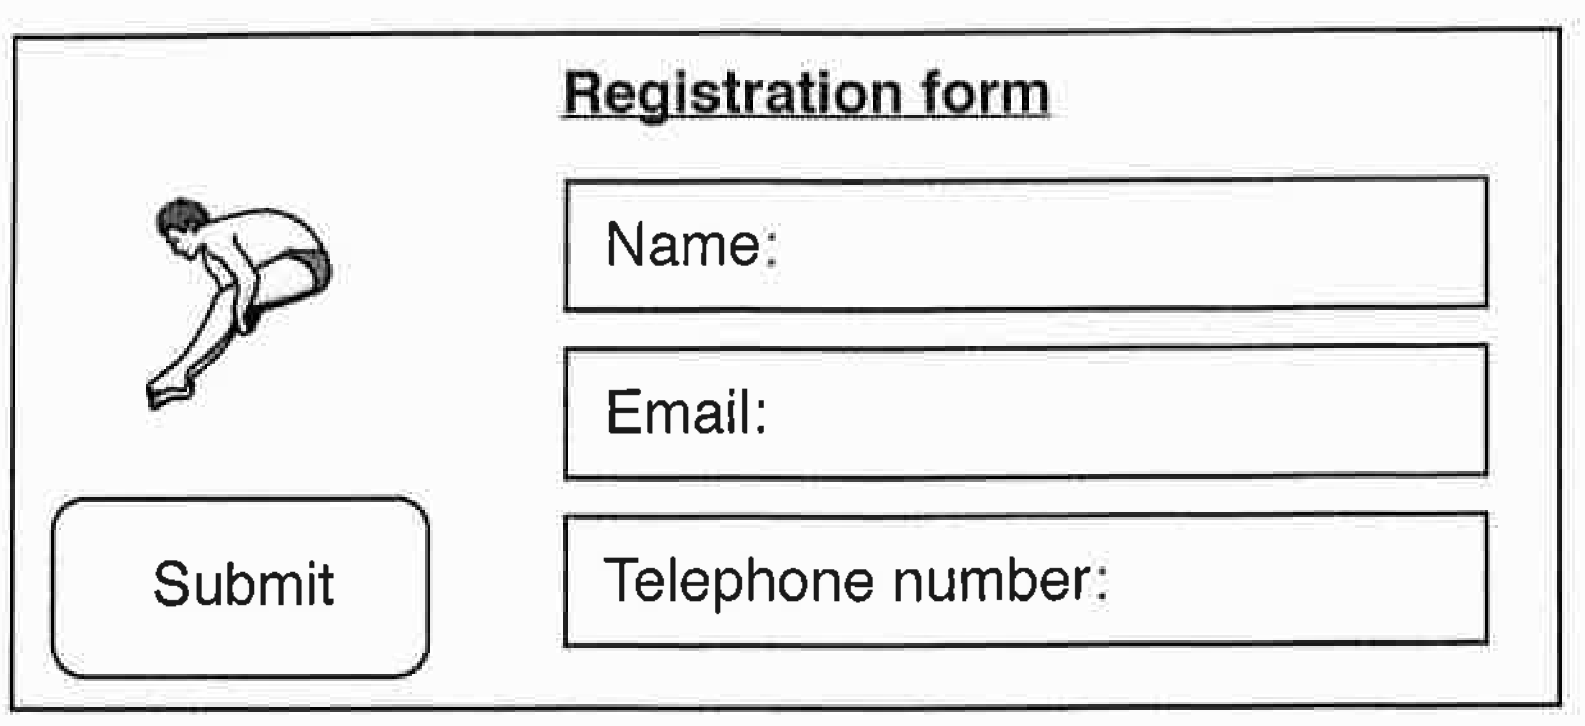
\includegraphics[width=0.5\paperwidth]{C:/Users/Admin/Desktop/Github/question_bank/LyX/static/img/9597-ALVL-2018-P2-Q6-2}
\par\end{center}

Explain how the web server will use server-side script to process
this form. \hfill{} {[}5{]}
\item The organisers of the championship store all the data for the event
using cloud storage. 

Describe\textbf{ three} economic benefits to the organisers of using
cloud-based storage. \hfill{}{[}3{]}
\end{enumerate}

 \newpage 

\item \textbf{{[}DHS/PRELIM/9597/2018/P1/Q1{]} }

The file \texttt{LOG.TXT} contains the access log entries of an organisation's
website from 0000 to 1800 hours on 1 August 2018.

The entries have the following format: 
\begin{enumerate}
\item[1.]  \textbf{host} (domain name or IP address) making the request.
\item[2.]  \textbf{timestamp} in the format \textquotedbl DAY MON DD HH:MM:SS
YYYY\textquotedbl , where \textbf{DAY} is the day of the week, \textbf{MON}
is the name of the month, \textbf{DD} is the day of the month, \textbf{HH:MM:SS}
is the time of day using a 24-hour clock, and \textbf{YYYY} is the
year. The timezone is -0400.
\item[3.]  \textbf{request} in quotes. 
\item[4.]  \textbf{HTTP reply status code}. 
\item[5.]  \textbf{bytes in the reply}.
\end{enumerate}

\subsection*{Task 1.1 }

Determine the top 5 hosts which accessed the website during this period,
in descending frequency order.

Sample output: 

\noindent %
\noindent\begin{minipage}[t]{1\columnwidth}%
\texttt{Top 5 hosts: }

\texttt{1 139.230.35.135 ~~~~~~~~~~~187}

\texttt{2 ns2.sharp.co.jp ~~~~~~~~~~95 }

\texttt{3 194.157.109.130 ~~~~~~~~~~62 }

\texttt{3 ix-dfw12-08.ix.netcom.com 62 }

\texttt{4 piweba1y.prodigy.com ~~~~~55 }

\texttt{5 205.163.36.61 ~~~~~~~~~~~~30}%
\end{minipage}

\subsection*{Evidence 1 }

Program code.\hfill{} {[}9{]}

\subsection*{Evidence 2 }

Screenshot. \hfill{}{[}1{]}

\subsection*{Task 1.2}

Determine the host which returned the largest reply size and the largest
reply size.

Sample output: 

\texttt{slip4086.sirius.com 12345}

\subsection*{Evidence 3 }

Program code.\hfill{} {[}4{]}

\subsection*{Evidence 4 }

Screenshot. \hfill{}{[}1{]}

 \newpage 

\item \textbf{{[}DHS/PRELIM/9597/2018/P1/Q2{]} }

A media access control (MAC) address is a unique identification code
hardwired to and used to identify individual devices on the network,
and is often expressed using hexadecimal notation eg. \texttt{4c:21:d0:15:e3:ea}.

\subsection*{Task 2.1 }

Using top down design, write iterative program code to convert a given
MAC address to decimal notation. For MAC address \texttt{4c:21:d0:15:e3:ea},
its converted decimal notation will be \texttt{76:33:208:21:227:234}.

\subsection*{Evidence 5 }

Program code. \hfill{}{[}4{]}

\subsection*{Evidence 6}

Screenshot.\hfill{} {[}1{]}

\subsection*{Task 2.2}

Write recursive program code to convert a given MAC address to decimal
notation. Use the same MAC address \texttt{4c:21:d0:15:e3:ea} to test
your program code.

\subsection*{Evidence 7 }

Program code.\hfill{} {[}4{]}

\subsection*{Evidence 8 }

Screenshot. \hfill{}{[}1{]}

\subsection*{Task 2.3 }

Write program code to perform input validation for a MAC address.
Test your program with suitable test data.

\subsection*{Evidence 9 }

Program code. \hfill{}{[}3{]}

\subsection*{Evidence 10 }

Screenshots. \hfill{}{[}2{]}

 \newpage 

\item \textbf{{[}DHS/PRELIM/9597/2018/P1/Q3{]} }

A blockchain is a linked list of blocks where each block has the following
structure:
\begin{center}
\begin{tabular}{|l|l|l|}
\hline 
\multicolumn{3}{|c|}{Class\texttt{: Block}}\tabularnewline
\hline 
\multicolumn{3}{|c|}{Attributes}\tabularnewline
\hline 
\texttt{\hspace{0.01\columnwidth}}Identifier & \texttt{\hspace{0.01\columnwidth}}Data Type & \texttt{\hspace{0.05\columnwidth}}Description\tabularnewline
\hline 
\texttt{Data} & \texttt{String} & Block data\tabularnewline
\hline 
\texttt{PrevHash} & \texttt{String} & Hash of previous block\tabularnewline
\hline 
\texttt{CurrHash} & \texttt{String} & Hash of \texttt{Data} and \texttt{PrevHash}\tabularnewline
\hline 
\texttt{Next} & \texttt{Integer} & The next block pointer\tabularnewline
\hline 
\end{tabular}
\par\end{center}

The structure of the blockchain is as follows:
\begin{center}
\begin{tabular}{|l|l|l|}
\hline 
\multicolumn{3}{|c|}{Class\texttt{: BlockChain}}\tabularnewline
\hline 
\multicolumn{3}{|c|}{Attributes}\tabularnewline
\hline 
\texttt{\hspace{0.01\columnwidth}}Identifier & \texttt{\hspace{0.01\columnwidth}}Data Type & \texttt{\hspace{0.05\columnwidth}}Description\tabularnewline
\hline 
\texttt{ChainData} & \texttt{Array{[}1:20{]} of Block} & An array used to store the 20 blocks.\tabularnewline
\hline 
\texttt{Start} & \texttt{Integer} & Index for the genesis block.\tabularnewline
\hline 
\texttt{NextFreeBlock} & \texttt{Integer} & Index for the next available empty block.\tabularnewline
\hline 
\end{tabular}
\par\end{center}

The initial value of \texttt{Start} is 1 and the initial value of
\texttt{NextFreeBlock} is 1.

The first block of the blockchain is called the genesis block and
its \texttt{PrevHash} value is 983.

The blockchain is used to store the achievement data of students in
computing and infocomm programmes. The ensures the integrity and verifiability
of students' portfolios which will be useful in internships, higher
education and career opportunities.

\subsection*{Task 3.1}

Write program code to declare and initialise an empty blockchain of
20 unused blocks. Also write the \texttt{Display} method to show all
contents of the blockchain.

\subsection*{Evidence 11}

Program code. \hfill{}{[}8{]}

\subsection*{Evidence 12 }

Screenshot. \hfill{}{[}2{]}

\subsection*{Task 3.2 }

The following hashing algorithm computes the \texttt{CurrHash} value
of each block: 
\begin{itemize}
\item Compute the sum of ASCII values for the characters in the achievement
data string. 
\item Multiply this sum by the kth prime number, where k is the length of
the achievement data string. 
\item Multiply this with the decimal equivalent of the \texttt{PrevHash}
value of the current block. 
\item Convert this value to its uppercase hexadecimal equivalent. 
\item Prepend the appropriate number of \texttt{'F'} to this result to form
a 23-character resultant string. This will be the current block's
\texttt{CurrHash} value.
\end{itemize}
For example, for the achievement data string
\noindent \begin{center}
\texttt{Splash Awards 2018:Robert Goh,Mary Tan,Choo Ah Beng:First }
\par\end{center}

Its \texttt{CurrHash} value will be \texttt{FFFFFFFFFFFFFFF4D32A036}
(sum of ASCII value {*} 57th prime number {*} \texttt{PrevHash} =
4898 {*} 269 {*} 983)

Write program code for a \texttt{ComputeHash} function to calculate
the \texttt{CurrHash} value of a block. Verify your function with
the following 2 achievement data strings:

\noindent %
\noindent\begin{minipage}[t]{1\columnwidth}%
\texttt{Splash Awards 2018:Robert Goh,Mary Tan,Choo Ah Beng:First}

\texttt{Splash Awards 2018:Lim Ah Huat,Alice Wong,Tan Ah Lian:Honorable
Mention}%
\end{minipage}

\subsection*{Evidence 13 }

Program code. \hfill{}{[}18{]}

\subsection*{Evidence 14}

Screenshot for the 2 achievement data strings. \hfill{}{[}2{]}

\subsection*{Task 3.3 }

Write program code to insert the data in \texttt{ACHIEVEMENTS.TXT}
into the blockchain and display the contents of the updated blockchain.

\subsection*{Evidence 15}

Program code.\hfill{} {[}4{]}

\subsection*{Evidence 16}

Screenshot. \hfill{}{[}1{]}

\subsection*{Task 3.4}

Lim Ah Huat aspires to save the world by studying computer science
in NUS School of Computing. As it is now the toughest course to get
admitted to, he hopes to improve his chances of admission by showcasing
his achievements in the various computing and infocomm related programmes
he has participated in. He claimed that he is a good team player and
is a strong self-directed learner with excellent aptitude for Computing.

How can the university admission panel verify his achievements using
the existing blockchain? You should describe briefly in program comments
this strategy and implement the associated program code.

\subsection*{Evidence 17 }

Program code. \hfill{}{[}5{]}

\subsection*{Evidence 18}

Screenshot.\hfill{} {[}1{]}

\subsection*{Task 3.5 }

Another student Tan Ah Seng claimed that he also has computing or
infocomm related participation, and changes one of the achievement
data string from 

\texttt{Splash Awards 2018:Lim Ah Huat,Alice Wong,Tan Ah Lian:Honorable
Mention}

to

\texttt{Splash Awards 2018:Lim Ah Huat,Alice Wong,Tan Ah Seng:Honorable
Mention}

Using program comments, briefly explain the impact to the blockchain.
Write program code to refute Mr Tan's claim.

\subsection*{Evidence 19 }

Program code. \hfill{}{[}3{]}

\subsection*{Evidence 20 }

Screenshot.\hfill{} {[}1{]}

 \newpage 

\item \textbf{{[}DHS/PRELIM/9597/2018/P1/Q4{]} }

Vector and matrix manipulation are used extensively in machine learning
programs. We will look at how common vector and matrix operations
are implemented using first principles 

\textbf{Addition and subtraction}

\texttt{{[}a,b,c{]} + {[}d,e,f{]} = {[}a+d,b+e,c+f{]}}

\texttt{{[}a,b,c{]} - {[}d,e,f{]} = {[}a-d,b-e,c-f{]}}

\textbf{Scalar multiplication} i.e. product of a constant and a vector 

\texttt{k {*} {[}a,b,c{]} = {[}k{*}a,k{*}b,k{*}c{]}}

\textbf{Dot product} (for 2 vectors of the same dimension)

\texttt{{[}a,b,c{]} $\cdot$ {[}d,e,f{]} = a{*}d + b{*}e + c{*}f}

\textbf{Distance} (between 2 vectors \texttt{{[}a,b,c{]}} and \texttt{{[}d,e,f{]}}
of the same dimension) 

$\sqrt{\left(\mathtt{a-d}\right)^{2}+\left(\mathtt{b-e}\right)^{2}+\left(\mathtt{c-f}\right)^{2}}$

\subsection*{Task 4.1 }

Using OOP techniques, create a class \texttt{Vector} to implement
the operations add, subtract, scalar multiplication, dot product and
distance. 

Exercise your class methods with the following vectors and constant: 

\texttt{v1 = {[}1,3,5{]}, v2 = {[}2,4,6{]}, k = 5}

\subsection*{Evidence 21 }

Program code. \hfill{}{[}12{]}

\subsection*{Evidence 22}

Screenshots. \hfill{}{[}2{]}

\subsection*{Task 4.2}

In some situations, it may be necessary to perform operations on vectors
of different dimensions eg for a convolution layer in deep learning.
The following diagram illustrates this process for a 3-element vector
\texttt{{[}1,2,3{]}} and a 5-element vector \texttt{{[}5,4,3,2,1{]}}.
The result will be a 3-element vector.
\begin{center}
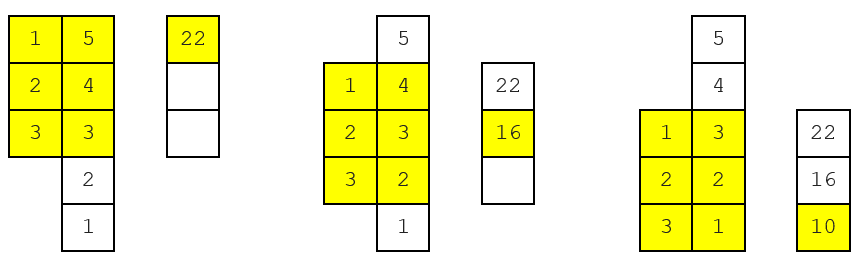
\includegraphics[width=0.5\paperwidth]{C:/Users/Admin/Desktop/Github/question_bank/LyX/static/img/9597-DHS-2018-P1-Q4-1}
\par\end{center}

Write program code to implement the convolution process for vectors.
Display the result to the screen.

\subsection*{Evidence 23 }

Program code. \hfill{}{[}5{]}

\subsection*{Evidence 24 }

Screenshot.\hfill{} {[}1{]}

\subsection*{Task 4.3 }

An example of the inner product for a matrix (2D array) is as follows:
\begin{center}
\includegraphics[width=0.5\paperwidth]{C:/Users/Admin/Desktop/Github/question_bank/LyX/static/img/9597-DHS-2018-P1-Q4-2}
\par\end{center}

Write program code to implement the convolution process for matrices
which uses the dot product for matrices. An example is shown below.
Display the result to the screen.
\begin{center}
\includegraphics[width=0.65\paperwidth]{C:/Users/Admin/Desktop/Github/question_bank/LyX/static/img/9597-DHS-2018-P1-Q4-3}
\par\end{center}

\subsection*{Evidence 25 }

Program code. \hfill{}{[}8{]}

\subsection*{Evidence 26}

Screenshot.\hfill{} {[}2{]}

 \newpage 

\item \textbf{{[}DHS/PRELIM/9597/2018/P2/Q1{]} }

The Singapore Quick Response Code (SGQR) is a single QR code that
combines multiple e-payment solutions into one. It is intended to
simplify QR e-payments in Singapore for both consumers and merchants.

Currently, consumers see multiple QR codes at merchant stores promoting
various e-payment solutions. This can be confusing for consumers who
have to manually find if their preferred e-payment option is accepted.
Merchants are also impacted by the aesthetic and logistics constraints
of supporting multiple QR codes on their limited display and retail
space. With SGQR, consumers will see a single SGQR label that shows
all QR payment options that the merchant accepts. For merchants, SGQR
will be an infrastructure-light and cheaper way to accept multiple
types of e-payments.
\begin{center}
\includegraphics[width=0.25\paperwidth]{C:/Users/Admin/Desktop/Github/question_bank/LyX/static/img/9597-DHS-2018-P2-Q1}
\par\end{center}

Merchants that currently offer QR code payments will have their existing
QR codes replaced with a single SGQR label over the next six months.
The first phase of SGQR label replacement, starting with merchants
in the Central Business District, will be commencing in late September
2018.
\begin{enumerate}
\item You have been engaged as a project manager to oversee the implementation
of SGQR in Dunman High School (DHS) canteen. Produce a project proposal
outlining the key activities to make DHS canteen cashless by March
2019. Your proposal should include the essential elements such as
problem statement, project management processes and tools (e.g. PERT
chart and Gantt chart), roles of team members, etc. \hfill{}{[}19{]}
\item Beyond SGQR and in line with the Smart Nation drive, you have also
engaged a systems analyst to come up with an online food ordering
application to allow students and staff to avoid long queues and streamline
the food preparation process using their mobile devices. The school
management also wishes to keep track of the situation to provide feedback
to the canteen vendors. 

Outline the deliverables in the various phases of the software development
life cycle (specification, design, development, documentation, implementation,
testing/modification and maintenance). Be sure to adapt your answer
to the question context. \hfill{}{[}12{]}
\item Networking is critical in such a project/system. Give an example of
where each of the following networking concept is applicable in your
project/system.
\begin{enumerate}
\item synchronous and asynchronous data transmission
\item simplex, half duplex and full duplex mode of data transmission
\item packet switching and circuit switching for data transmission \hfill{}{[}6{]}
\end{enumerate}
\item You are also mindful about and is determined to prevent cybersecurity
attacks like the recent SingHealth data breach of the personal information
of 1.5 million patients. Outline a comprehensive organisational security
plan which goes beyond technical controls (user authentication, access
levels, antivirus, firewalls) to ensure that both the hardware infrastructure
and software applications are well secured against cybersecurity hacks.\hfill{}
{[}8{]}
\end{enumerate}

 \newpage 

\item \textbf{{[}DHS/PRELIM/9597/2018/P2/Q2{]} }

Mergesort uses a divide and conquer approach to successively divide
a list into half, forming two sublists, until each sublist is of length
1. The sublists are then sorted and merged into larger sublists until
they are recombined into a single sorted list. An algorithm for mergesort
is given below.

\noindent %
\noindent\begin{minipage}[t]{1\columnwidth}%
\texttt{procedure mergesort(mergelist)}

\texttt{\qquad{}if len(mergelist) > 1 then }

\texttt{\qquad{}\qquad{}mid = len(mergelist) div 2}

\texttt{\qquad{}\qquad{}lefthalf = mergelist{[}:mid{]}}

\texttt{\qquad{}\qquad{}righthalf = mergerlist{[}mid:{]}}

\texttt{\bigskip{}
}

\texttt{\qquad{}\qquad{}mergesort(lefthalf) }

\texttt{\qquad{}\qquad{}mergesort(righthalf)}

\texttt{\bigskip{}
}

\texttt{\qquad{}\qquad{}i = 0}

\texttt{\qquad{}\qquad{}j = 0}

\texttt{\qquad{}\qquad{}k = 0 }

\texttt{\qquad{}\qquad{}while i < len(lefthalf) and i < len(righthalf)}

\texttt{\qquad{}\qquad{}\qquad{}if lefthalf{[}i{]} < righthalf{[}j{]}
then}

\texttt{\qquad{}\qquad{}\qquad{}\qquad{}mergelist{[}k{]} = lefthalf{[}i{]}}

\texttt{\qquad{}\qquad{}\qquad{}\qquad{}i = i + 1 }

\texttt{\qquad{}\qquad{}\qquad{}else}

\texttt{\qquad{}\qquad{}\qquad{}\qquad{}mergelist{[}k{]} = righthalf{[}j{]} }

\texttt{\qquad{}\qquad{}\qquad{}\qquad{}j = j + 1}

\texttt{\qquad{}\qquad{}\qquad{}endif }

\texttt{\qquad{}\qquad{}\qquad{}k = k + 1 }

\texttt{\qquad{}\qquad{}endwhile }

\texttt{\bigskip{}
}

\texttt{\qquad{}\qquad{}while i < len(lefthalf) }

\texttt{\qquad{}\qquad{}\qquad{}mergelist{[}k{]} = lefthalf{[}i{]}}

\texttt{\qquad{}\qquad{}\qquad{}i = i + 1}

\texttt{\qquad{}\qquad{}\qquad{}k = k + 1 }

\texttt{\qquad{}\qquad{}endwhile}

\texttt{\qquad{}\qquad{}while j < len(righthalf)}

\texttt{\qquad{}\qquad{}\qquad{}mergelist{[}k{]} = righthalf{[}j{]}}

\texttt{\qquad{}\qquad{}\qquad{}j = j + 1}

\texttt{\qquad{}\qquad{}\qquad{}k = k + 1 }

\texttt{\qquad{}\qquad{}endwhile}

\texttt{\qquad{}endif }

\texttt{endprocedure}%
\end{minipage}
\begin{enumerate}
\item The following list of numbers is to be sorted using mergesort:

\texttt{mergelist = {[}5, 3, 2, 7, 9, 1, 3, 8{]}}

What are the first two lists to be merged? \hfill{}{[}2{]}
\item Draw a graphical representation of how the above list is first split
into halves until each sublist contains zero or one items, and then
the sublists are merged to become the sorted list. \hfill{}{[}4{]}
\item Give and justify the time complexity of mergesort. \hfill{}{[}2{]}
\item Compare the space complexities of mergesort and quicksort.\hfill{}
{[}2{]}
\end{enumerate}

 \newpage 

\item \textbf{{[}DHS/PRELIM/9597/2018/P2/Q3{]} }
\begin{enumerate}
\item Devise an algorithm to sort a list of words so that the anagrams are
grouped together.

For example, if the unsorted list is 

tar, phone, rat

after sorting we should get

tar, rat, phone

since tar and rat are anagrams, they are grouped together.\hfill{}{[}5{]}
\item Devise an algorithm to find the length of the longest palindrome in
a string s. \hfill{}{[}5{]}
\end{enumerate}

 \newpage 

\item \textbf{{[}DHS/PRELIM/9597/2018/P2/Q4{]} }

A program needs to be written to store and manage product information.
The program will have the following functionality:
\begin{itemize}
\item able to display a list of products in alphabetical order 
\item able to support efficient additions and deletions 
\item able to search for a product efficiently
\end{itemize}
\begin{enumerate}
\item Explain why it is better to use a binary search tree (BST) than an
ordered array to store and manage product information\hfill{}. {[}2{]}

The initial list of products to be stored are: 
\noindent \begin{center}
battery, cable, detergent, medicine, soap, towel, yoyo
\par\end{center}
\item Draw the BST 
\begin{enumerate}
\item from the initial list to support efficient seach, addition and deletion 
\item when new items earphone and eraser have been inserted in that order
\item when medicine has been deleted \hfill{}{[}5{]}
\end{enumerate}
\item State the postorder traversal output of the updated BST. \hfill{}{[}1{]}
\item Outline how the BST can be reorganised after a series of additions
and deletions to ensure optimal search performance.\hfill{} {[}2{]}
\end{enumerate}

 \newpage 

\item \textbf{{[}DHS/PRELIM/9597/2018/P2/Q5{]} }

A digital media company currently sells electronic books and audio
books. Each book has a unique id, title, image and price. An electronic
book has a default number of pages while an audio book has a duration. 
\begin{enumerate}
\item Draw a class diagram showing the relationship between the different
digital book types. \hfill{}{[}3{]}
\item Using appropriate examples, explain the following terms:
\begin{enumerate}
\item encapsulation
\item inheritance
\item polymorphism\hfill{} {[}6{]}
\end{enumerate}
\item To improve sales, the company decides to
\begin{enumerate}
\item Offer discounts on selected book items. Discounts on each book may
vary from 0 to 50\%.
\item sell digital movies. Each movie has a duration as well as a rating
with possible values G, PG and PG13. 
\item offer a monthly subscription service with unlimited access to all
digital media.
\end{enumerate}
Explain how these changes will affect your design in \textbf{part
(a)}. \hfill{}{[}6{]}
\end{enumerate}

 \newpage 

\item \textbf{{[}DHS/PRELIM/9597/2018/P2/Q6{]} }

The following figure shows the partial contents of an unnormalised
relational database table for library book loans by an amateur database
administrator. 
\noindent \begin{center}
\begin{tabular}{|c|c|c|c|c|c|c|c|c|}
\hline 
CallNo & Title & Author & PublisherID & PublisherName & BorrowerID & BorrowerName & Email & LoanDate\tabularnewline
\hline 
A2345 & Superhuman & Peter Smith & P0928 & Healthy Global & X894 & Robert Lim & roblim@gmail.com & 20181004\tabularnewline
\hline 
A1133 & Agile Methodology & Sophia Jones & P7823 & CS Books & X894 & Robert Lim & roblim@gmail.com & 20181004\tabularnewline
\hline 
B5104 & Python Advanced & Zen Wang & P8246 & Make It Harder & Y532 & Mary Tan & maryt@yahoo.com & 20181007\tabularnewline
\hline 
A2257 & Computer Science & Berry Mile & P8246 & Make It Harder & X451 & Ben Neo & benn@gmail.com & 20181007\tabularnewline
\hline 
B7513 & Alibaba & Jacky Ma & P3245 & Ali Pub  & X451 & Ben Neo & benn@gmail.com & 20181007\tabularnewline
\hline 
\end{tabular}
\par\end{center}

\begin{enumerate}
\item Give \textbf{two} potential anomalies that can occur with this design.
\hfill{}{[}2{]}
\item Give \textbf{two} advantages of normalisation. \hfill{}{[}2{]}
\item Give the table specification in 
\begin{enumerate}
\item 1NF
\item 2NF
\item 3NF \hfill{}{[}6{]}
\end{enumerate}
\item Draw an E-R diagram to represent your normalised design.\hfill{}
{[}3{]}
\item The following figure shows the notification email sent to the borrower
upon successful loan of library books.

\noindent\fbox{\begin{minipage}[t]{1\columnwidth - 2\fboxsep - 2\fboxrule}%
\texttt{Oct 4, 2018, 6:52 PM }

\texttt{From: NLB <helpdesk@nlb.gov.sg> }

\texttt{To: roblim@gmail.com}

\bigskip{}

\texttt{Dear Robert Lim}

\bigskip{}

\texttt{Thank you for using NLB's e-notification service through email,
a free service available to all library members.}

\bigskip{}

\texttt{This notification service confirms the number of items you
have borrowed at the library book borrowing station.}

\bigskip{}

\texttt{You have borrowed 2 item(s) at 18:52 on 4 Oct 2018 at Serangoon
Public Library:}

\bigskip{}

\texttt{1. Superhuman }

\texttt{~~~Due on: 25 October 2018}

\bigskip{}

\texttt{2. Agile Methodology }

\texttt{~~~Due on: 25 October 2018}

\bigskip{}

\texttt{You may also check your updated account status at http://www.nlb.gov.sg}%
\end{minipage}}

Describe how the customised contents of the notification email are
generated from the database. You may assume that the default loan
period is 21 days.\hfill{} {[}3{]}
\end{enumerate}

 \newpage 

\item \textbf{{[}DHS/PRELIM/9597/2018/P1/Q1{]} }

A programmer is writing a treasure island game to be played on the
computer. 

The island is a rectangular grid, 30 squares by 10 squares. Each square
of the island is represented by an element in a 2D array. The top
left square of the island is represented by the array element {[}0,
0{]}.

There are 30 squares across and 10 squares down. 

The computer will: 
\begin{itemize}
\item generate three random locations where treasure will be buried 
\item prompt the player for the location of one square where the player
choose to dig
\item display the contents of the array by outputting for each square: 
\begin{itemize}
\item '.' for only sand in this square
\item 'T' for treasure still hidden in sand 
\item 'X' for a hole dug where treasure was found
\item 'O' for a hole dug where no treasure was found. 
\end{itemize}
\end{itemize}
Here is an example display after the player has chosen to dig at location
{[}9, 3{]}: 

\noindent %
\noindent\begin{minipage}[t]{1\columnwidth}%
\texttt{.............................. }

\texttt{.............................. }

\texttt{.............................. }

\texttt{.............................. }

\texttt{..................T........... }

\texttt{.............................. }

\texttt{...T.......................... }

\texttt{.............................. }

\texttt{.............................. }

\texttt{...X..........................}%
\end{minipage}

The game is to be implemented using object oriented programming. 

The programmer has designed the class \texttt{IslandClass}. The identifier
table for this class is: 
\begin{itemize}
\item \texttt{Grid : ARRAY{[}0:9, 0:29{]} OF CHAR} - 2D array to represent
the squares of the island 
\item \texttt{Constructor()} - instantiates an object of class \texttt{IslandClass}
and initialises all squares to sand 
\item \texttt{HideTreasure()} - generates a pair of random numbers used
as the grid location of treasure and marks the square with \texttt{'T'} 
\item \texttt{DigHole(Row, Column)} - takes as parameter a valid grid location
and marks the square with \texttt{'X'} or \texttt{'O'} as appropriate 
\item \texttt{GetSquare(Row, Column) : CHAR} - takes as parameter a valid
grid location and returns the grid value for that square from the
\texttt{IslandClass} object 
\item \texttt{DisplayGrid()} - shows the current grid data. \texttt{DisplayGrid}
should make use of the getter method \texttt{GetSquare} of the \texttt{IslandClass}
class
\end{itemize}

\subsection*{Task 1.1 }

Write program code for the class \texttt{IslandClass} including the
\texttt{Constructor}, \texttt{GetSquare} and \texttt{DisplayGrid}
methods. The code should follow the specification given. 

The value to represent sand should be declared as a constant. Do not
attempt to write the methods \texttt{HideTreasure} or \texttt{DigHole}
at this stage.

\subsection*{Evidence 1}

Program code for Task 1.1\hfill{} {[}5{]}

\subsection*{Task 1.2 }

Write program code for the \texttt{HideTreasure} method. Your method
should check that the random location generated does not already contain
treasure. The value to represent treasure should be declared as a
constant. 

\subsection*{Evidence 2 }

Your program code for Task 1.2\hfill{} {[}3{]}

\subsection*{Task 1.3 }

Write a main program to: 
\begin{itemize}
\item create an IslandClass object 
\item generate three random locations where treasures will be buried
\item your program will then call the DisplayGrid method. 
\end{itemize}

\subsection*{Evidence 3 }

The program code for Task 1.3 \hfill{}{[}3{]}

\subsection*{Evidence 4}

Screenshot showing the output from running the program in Task 1.3\hfill{}
{[}1{]}

\subsection*{Task 1.4 }

Write program code for the \texttt{DigHole} method. This method takes
two integers as parameters. These parameters form a valid grid location.
The location is marked with \texttt{'X'} or \texttt{'O'} as appropriate. 

The values to represent treasure, found treasure and hole should be
declared as constants. 

\subsection*{Evidence 5}

Program code for Task 1.4. \hfill{}{[}3{]}

\subsection*{Task 1.5 }

Add code to the main program in Task 1.3. The program is to: 
\begin{itemize}
\item prompt the player for a location to dig 
\item validate the user input
\item call the \texttt{DigHole} method and then the \texttt{DisplayGrid}
method. 
\end{itemize}

\subsection*{Evidence 6 }

The program code.\hfill{} {[}3{]}

\subsection*{Task 1.6}

Run the program by inputting a location where: 
\begin{itemize}
\item the treasure is not found
\item the treasure is found. 
\end{itemize}

\subsection*{Evidence 7}

Screenshot evidence similar to that shown which shows: 
\begin{itemize}
\item The player has chosen to dig at location {[}2, 25{]} where no treasure
was found 

\noindent\begin{minipage}[t]{1\columnwidth}%
\texttt{.............................. }

\texttt{....T......................... }

\texttt{.........................O.... }

\texttt{..............................}

\texttt{..........T................... }

\texttt{.............................. }

\texttt{..................T........... }

\texttt{.............................. }

\texttt{.............................. }

\texttt{..............................}%
\end{minipage}
\item The player has chosen to dig at location {[}5, 3{]} where treasure
was found 

\noindent\begin{minipage}[t]{1\columnwidth}%
\texttt{.............................. }

\texttt{..............................}

\texttt{...............T..............}

\texttt{.............................. }

\texttt{.........................T.... }

\texttt{...X.......................... }

\texttt{.............................. }

\texttt{..............................}

\texttt{.............................. }

\texttt{..............................}%
\end{minipage}

\hfill{} {[}2{]}
\end{itemize}

 \newpage 

\item \textbf{{[}DHS/PRELIM/9597/2018/P1/Q2{]} }

The International Bank Account Number (IBAN) is an international bank
account identification standard used in many countries. It uses modulo
arithmetic to perform validation. The IBAN consists of up to 34 alphanumeric
characters, as follows: country code -- two letters check digits
-- two digits, and basic bank account number -- up to 30 alphanumeric
characters that are countryspecific An example of an IBAN in the United
Kingdom Great Britain which is 22 characters is \texttt{GB82WEST12345698765432}
(\texttt{GB} - country code, \texttt{82} - check digits) 

The following is the IBAN check digits generation algorithm: 
\begin{enumerate}
\item[1.]  Initialize the two check digits by \texttt{00} (e.g. \texttt{GB}\texttt{\uline{00}}\texttt{WEST12345698765432}).
\item[2.]  Move the four initial characters to the end of the string (e.g.
\texttt{WEST12345698765432GB}\texttt{\uline{00}}). 
\item[3.]  Replace each alphabet in the string with two digits, using the mapping
A = 10, B = 11, C = 12, . . . . . , Z = 35 (i.e. ASCII value of uppercase
letters - 55) (e.g. \texttt{\uline{32142829}}\texttt{12345698765432}\texttt{\uline{1611}}\texttt{00}). 
\item[4.]  Convert the string to an integer. 
\item[5.]  Calculate the remainder of dividing this number by 97 (e.g. \texttt{3214282912345698765432161100
mod 97 = 16}).
\item[6.]  Subtract the remainder from 98 to give the two check digits (e.g.
check digits \texttt{= 98 - 16 = 82}). If the result is a single digit
number, pad it with a leading 0 to make a two-digit number. 
\end{enumerate}

\subsection*{Task 2.1 }

Write program code for the \texttt{CheckDigits} function using the
following specification. 
\noindent \begin{center}
\texttt{FUNCTION CheckDigits (IBAN : STRING) : STRING }
\par\end{center}

The function has a single string parameter IBAN and returns a two-digit
string result. Use the sample data provided in the text file \texttt{IBANS.txt}
and paste this into your program code.

\subsection*{Evidence 8 }

Your program code. \hfill{}{[}6{]}

\subsection*{Evidence 9 }

One screenshot verifying that your program generates the correct check
digits for the data in \texttt{IBANS.txt}. \hfill{}{[}1{]}

An IBAN is validated by converting it into an integer and performing
a basic mod-97 operation on it. If the IBAN is valid, the remainder
equals 1. The algorithm of IBAN validation is as follows:
\begin{enumerate}
\item[1.]  Move the four initial characters to the end of the string (For the
IBAN \texttt{GB82WEST12345698765432} e.g. \texttt{WEST12345698765432}\texttt{\uline{GB82}}).
\item[2.]  Replace each letter in the string with two digits, thereby expanding
the string, where A = 10, B = 11, C = 12, . . . . . , Z = 35 

(e.g. \texttt{\uline{32142829}}\texttt{12345698765432}\texttt{\uline{1611}}\texttt{82}). 
\item[3.]  Interpret the string as a decimal integer and compute the remainder
of that number on division by 97 

(e.g. \texttt{3214282912345698765432161182 mod 97 = 1}). 
\end{enumerate}
If the remainder is 1, the check digit test is passed and the IBAN
might be valid.

\subsection*{Task 2.2 }

Write a Boolean function \texttt{ValidateIBAN} to determine if a given
IBAN is valid. This function should have a parameter which allows
it to be used for any IBAN. 

\subsection*{Evidence 10 }

Your \texttt{ValidateIBAN} program code. \hfill{}{[}2{]}

\subsection*{Task 2.3 }

A \texttt{TRANSACTIONS.txt} file contains transaction details of customers
of a bank. Each transaction record takes up one line and has three
data fields: customer IBAN, transaction mode (\texttt{W} - withdrawal
or \texttt{D} - deposit) and transaction amount. 

Write a procedure \texttt{CheckIBAN} to read in the IBANs in \texttt{TRANSACTIONS.txt}
and display on the screen: 
\begin{itemize}
\item If an IBAN is valid, the valid IBAN followed by \textquotedblleft \texttt{OK}\textquotedblright . 
\item If an IBAN is invalid, the invalid IBAN followed by \texttt{\textquotedblleft Invalid. Expected
check digits: ??\textquotedblright }, where ?? represents the computed
check digits. 
\item For an invalid IBAN, update the record in \texttt{TRANSACTIONS.txt}
with the expected computed check digits.
\end{itemize}

\subsection*{Evidence 11 }

Your \texttt{CheckIBAN} program code.\hfill{} {[}7{]}

\subsection*{Evidence 12 }

One screenshot showing the output and contents of \texttt{TRANSACTIONS.txt}
from running the program. {[}2{]} 

\subsection*{Task 2.4 }

A master file \texttt{ACCOUNTS.txt} contains the customer IBANs, names
and current balances. 

Write a procedure \texttt{UpdateBalance} to update the current balances
of the customers in \texttt{ACCOUNTS.txt} from \texttt{TRANSACTIONS.txt}.
At the end of the process, your program will output the message: 

\texttt{x records updated. }

\subsection*{Evidence 13}

Your program code for the procedure \texttt{UpdateBalance}.\hfill{}
{[}8{]}

\subsection*{Evidence 14}

One screenshot showing the program output and contents of \texttt{ACCOUNTS.txt}
from running the program.\hfill{} {[}2{]}

 \newpage 

\item \textbf{{[}DHS/PRELIM/9597/2018/P1/Q3{]} }

A linked list Abstract Data Type (ADT) has the following operations
defined: 
\begin{itemize}
\item \texttt{Create()} -{}- creates an empty linked list; 
\item \texttt{Insert(item, p)} -{}- inserts new value, \texttt{item}, into
linked list so that it is at position \texttt{p} in the linked list.
Assume that the linked list contains at least \texttt{(p - 1)} items
before the insertion. 
\item \texttt{Delete(p)} -{}- deletes the item at position \texttt{p} in
the linked list; 
\item \texttt{Length()} -{}- returns the number of items in the linked list; 
\item \texttt{IsEmpty()} -{}- returns \texttt{True} if linked list is empty; 
\item \texttt{IsFull()} -- returns \texttt{True} if linked list is full; 
\end{itemize}
The linked list is implemented by the use of a collection of nodes
that have two parts: the item data and a pointer to the next item
in the list. In addition there is a \texttt{Start} pointer which points
to the first item in the list. 

The unused nodes are linked and the first unused node is the position
where the next new data item is to be stored. Node removed from the
linked list should be returned to \texttt{NextFree} list.
\begin{center}
\includegraphics[width=0.65\paperwidth]{static/img/9597-HCI-2018-P1-Q3-1}
\par\end{center}

The diagram shows the linked list after the following sequence of
commands have been executed. 

\noindent\begin{minipage}[t]{1\columnwidth}%
\texttt{Create() }

\texttt{Insert('Ali', 1) }

\texttt{Insert('Jack', 1)}

\texttt{Insert('Ben',2)}

\texttt{Delete(1) }

\texttt{Insert('Jane', 2) }

\texttt{Insert('Ken', 3)}

\texttt{Delete(2)}%
\end{minipage}

The program to implement this ADT will use the classes \texttt{ListNode}
and \texttt{LinkedList} as follows: 
\begin{center}
\begin{tabular}{|l|}
\hline 
\hspace{0.25\columnwidth}\texttt{ListNode}\tabularnewline
\hline 
\texttt{Name : STRING}\tabularnewline
\texttt{Pointer : INTEGER}\tabularnewline
\hline 
\texttt{Constructor()}\tabularnewline
\texttt{SetName(Name:STRING)}\tabularnewline
\texttt{SetPointer(Pointer:INTEGER)}\tabularnewline
\texttt{GetName():STRING}\tabularnewline
\texttt{GetPointer():INTEGER}\tabularnewline
\hline 
\end{tabular}
\par\end{center}

\begin{center}
\begin{tabular}{|l|}
\hline 
\hspace{0.25\columnwidth}\texttt{LinkedList}\tabularnewline
\hline 
\texttt{Node : ARRAY {[}1..10{]} OF ListNode}\tabularnewline
\texttt{Start : INTEGER NextFree : INTEGER}\tabularnewline
\hline 
\texttt{Constructor()}\tabularnewline
\texttt{Insert (name: STRING, position: INTEGER)}\tabularnewline
\texttt{Delete (position: INTEGER)}\tabularnewline
\texttt{Length (): INTEGER}\tabularnewline
\texttt{IsEmpty(): BOOLEAN}\tabularnewline
\texttt{IsFull() : BOOLEAN}\tabularnewline
\hline 
\end{tabular}
\par\end{center}

\subsection*{Task 3.1 }

Write program code to define the classes \texttt{ListNode} and \texttt{LinkedList}. 

\subsection*{Evidence 15}

Program code for the \texttt{ListNode} and \texttt{LinkedList} classes.
\hfill{}{[}18{]}

\subsection*{Task 3.2 }

A method \texttt{Display()} is to be added, which displays the value
of \texttt{Start}, the value of \texttt{NextFree} and the contents
of \texttt{Node} array in index order. Write program code to implement
this method.

\subsection*{Evidence 16}

Your program code for Task 3.2. \hfill{}{[}4{]}

\subsection*{Task 3.3 }

Write code to create a \texttt{LinkedList} object in the main program.
Paste the sequence of commands in \texttt{COMMANDS.txt} into your
program code. Your program will then call the \texttt{Display} method. 

Execute your program to test it.

\subsection*{Evidence 17 }

Screenshot showing the output from running the program in Task 3.3.
\hfill{}{[}2{]}

A linear queue is implemented using the \texttt{LinkedList} class
as a super class. 

The subclass \texttt{Queue} has the following methods: 
\begin{itemize}
\item \texttt{Enqueue(item)} -{}- inserts item at the rear of the queue;
\item \texttt{Dequeue()} -{}- deletes the item at the front of the queue; 
\item \texttt{Display()} -{}- displays the contents of the queue using the
format given below.
\noindent \begin{center}
\texttt{}%
\begin{tabular}{lcl}
\texttt{Steven} & \texttt{$\leftarrow$} & \texttt{Front}\tabularnewline
\texttt{Celine} &  & \tabularnewline
\texttt{Tom} &  & \tabularnewline
\texttt{Ryan} & \texttt{$\leftarrow$} & \texttt{Rear}\tabularnewline
 &  & \tabularnewline
\multicolumn{3}{l}{\texttt{Numbers in queue : 4}}\tabularnewline
\end{tabular}
\par\end{center}
\end{itemize}

\subsection*{Task 3.4 }

Write program code for the subclass \texttt{Queue}.

Use appropriate inheritance and polymorphism in your design. 

\subsection*{Evidence 18}

Your program code for Task 3.4. \hfill{} {[}5{]}

\subsection*{Task 3.5 }

Write program code to: 
\begin{itemize}
\item create a new queue and add the data in the file \texttt{NAMES.txt}
to the queue 
\item remove two items from the queue 
\item display final contents of the queue 
\end{itemize}

\subsection*{Evidence 19 }

Your program code for Task 3.5. \hfill{} {[}2{]}

\subsection*{Evidence 20}

Screenshot showing the output from running the program in Task 3.5.
\hfill{} {[}1{]}

 \newpage 

\item \textbf{{[}DHS/PRELIM/9597/2018/P1/Q4{]} }

The Romans had their own system of number representation which used
a sequence of upper case letter characters to represent a number.
We shall consider the denary number 1 to 20 only. 

The following letters represent each of the values shown: 
\noindent \begin{center}
\begin{tabular}{|c|c|}
\hline 
Roman Numeral  & Represents\tabularnewline
\hline 
I & One\tabularnewline
\hline 
V & Five\tabularnewline
\hline 
X & Ten\tabularnewline
\hline 
L & Fifty\tabularnewline
\hline 
\end{tabular}
\par\end{center}

A number is always written with the smallest number of characters,
with the letters in sequence starting with the character with the
largest value. 
\begin{itemize}
\item For example, 6 is written \texttt{VI} (not \texttt{IIIIII}) 
\end{itemize}
The exceptions to this sequence are as follows: 
\begin{itemize}
\item one less than 5 -{}- which is written as \texttt{IV}
\item one less than ten -{}- which is written as \texttt{IX} 
\item ten less than fifty -{}- which is written as \texttt{XL} 
\end{itemize}

\subsection*{Task 4.1}

Write program code with the following specification: Input a denary
integer number in the range 1 to 20 Validate the input Calculate the
Roman numeral representation (write this code as a function) Output
the Roman number. 

\subsection*{Evidence 21 }

Your program code. \hfill{}{[}6{]}

\subsection*{Task 4.2 }

Draw up a list of \textbf{three} suitable tests and provide screenshot
evidence for your testing.

\subsection*{Evidence 22 }

Annotated screenshots for each test data run.\hfill{} {[}3{]}

\subsection*{Task 4.3}

Write additional program code with appropriate data validation for
the following specification:
\begin{itemize}
\item Input two Roman numeral numbers between 1 and 20 
\item Ouput the sum of the numbers as a Roman numeral number.
\end{itemize}

\subsection*{Evidence 23 }

Your program code.\hfill{} {[}8{]}

\subsection*{Task 4.4 }

Draw up a list of \textbf{three} suitable tests and provide screenshot
evidence for your testing. 

\subsection*{Evidence 24 }

Annotated screenshots for each test data run. \hfill{}{[}3{]}

 \newpage 

\item \textbf{{[}DHS/PRELIM/9597/2018/P2/Q1{]} }
\begin{enumerate}
\item A local area network can be set up as either client-server or peer-to-peer.
\begin{enumerate}
\item State where data are stored on a client-server network and why? \hfill{}{[}1{]}
\item State where data are stored on a peer-to-peer network and why? \hfill{}{[}1{]}
\item In your opinion, what is the key benefit of a client-server network
over peer-topeer network. Justify. \hfill{}{[}2{]}
\item In your opinion, what is the main drawback of a client-server network
compared to a peer-to-peer network. Justify. \hfill{}{[}2{]}
\end{enumerate}
\item A 60 Megabyte file is transferred over a network to a printer in 10
seconds. 

Calculate the transfer rate, in kilobytes per second, used to transfer
this file. Show all of your working. {[}1 MB = 1024 KB{]} \hfill{}{[}2{]}
\item Explain how DHCP operates in a network? \hfill{}{[}3{]}
\item Switches and routers are both connecting devices.
\begin{enumerate}
\item What are the purposes of having connecting device in a network?\hfill{}
{[}2{]}
\item What are the differences between them?\hfill{} {[}2{]}
\end{enumerate}
\end{enumerate}

 \newpage 

\item \textbf{{[}DHS/PRELIM/9597/2018/P2/Q2{]} }
\begin{enumerate}
\item What are the characteristics of a voice-user interface? \hfill{}{[}2{]}
\item What are the strengths and weaknesses of a voice-user interface in
comparison to a graphical user-interface?\hfill{}{[}4{]}
\item One of the 8 golden rules for interface design is the element of consistency. 
\begin{enumerate}
\item Explain the importance of consistency in designing a user interface.
\hfill{}{[}4{]}
\item Is consistency still important in the newer user-interfaces (eg. voice,
gesture)? Why is this so?\hfill{} {[}2{]}
\item Voice User interfaces gaining popularity with the readily availablity
of devices like Echo and iphone. What do you think are some of the
key design elements that are vital to an effective user experience
when using such devices? Explain your answers.\hfill{} {[}3{]}
\end{enumerate}
\end{enumerate}

 \newpage 

\item \textbf{{[}DHS/PRELIM/9597/2018/P2/Q3{]} }
\begin{enumerate}
\item Explain what is meant by the following terms and give an example for
each
\begin{enumerate}
\item Candidate key\hfill{} {[}2{]}
\item Secondary key \hfill{} {[}2{]}
\item Foreign key\hfill{} {[}2{]}
\end{enumerate}
\item The school\textquoteright s Robotics club is looking at designing
a relational database to keep track of members participation and achievements.
Proposed a relational database design for this purpose.
\begin{enumerate}
\item Give the table descriptions in shorthand notations. Explain the purpose
of all your tables. Highlight the necessary details needed in your
design.\hfill{} {[}6{]}
\item Draw the entity-relationship model for your design.\hfill{} {[}3{]}
\end{enumerate}
\end{enumerate}

 \newpage 

\item \textbf{{[}DHS/PRELIM/9597/2018/P2/Q4{]} }

An apartment block in a city consists of a large number of apartments.
Each of the residents of the apartments has their information stored
in a file. 

The records in the file are to be sorted into alphabetical order of
the resident\textquoteright s name.
\begin{enumerate}
\item Using the following list of names as an example, show how the records
can be sorted into alphabetical order using an insertion sort. 

GRA, CHR, DAV, SAR, TOM, KAT \hfill{}{[}4{]}
\item Residents sometimes make requests for maintenance on their apartments.
Each request is given a priority number ranging from 1, for failure
of the air conditioning, to 10, for a dripping tap. Each request is
stored in a linked list in order of priorities. Jobs with equal priority
are stored in order of the date that they have been submitted. 

Describe an algorithm to insert a new job into the list.\hfill{}
{[}6{]}
\end{enumerate}

 \newpage 

\item \textbf{{[}DHS/PRELIM/9597/2018/P2/Q5{]} }
\begin{enumerate}
\item Explain the difference between an iterative solution and a recursive
solution to a problem. \hfill{}{[}2{]}
\item The program \texttt{RADIX\_CONVERT}, listed below, calls a recursive
procedure, OUT. Note that x DIV y gives the integral part of the quotient
when x is divided by y, and x MOD y gives the remainder. 

\noindent\begin{minipage}[t]{1\columnwidth}%
\texttt{Program RADIX\_CONVERT }

\texttt{\qquad{}declare integers a, b}

\texttt{\qquad{}input a, b OUT (a, b) }

\texttt{\qquad{}print a, b }

\texttt{End RADIX\_CONVERT }

\bigskip{}

\texttt{Procedure OUT (x, y) }

\texttt{\qquad{}declare integers a, b }

\texttt{\qquad{}a = x DIV y }

\texttt{\qquad{}b = x MOD y }

\texttt{\qquad{}if a > 0 then OUT (a, y) }

\texttt{\qquad{}print (b) }

\texttt{End OUT }%
\end{minipage}
\begin{enumerate}
\item Draw a diagram to trace the execution of the program, \texttt{RADIX\_CONVERT}
with values 46 and 3 as input for \texttt{a} and \texttt{b} respectively.
Show clearly the order of call and return, and the change in values
of a and b.\hfill{}{[}4{]}
\item Write down, in the correct order, all the values printed. \hfill{}{[}2{]}
\item What does \texttt{RADIX\_CONVERT} accomplish? \hfill{}{[}2{]}
\end{enumerate}
\end{enumerate}

 \newpage 

\item \textbf{{[}DHS/PRELIM/9597/2018/P2/Q6{]} }

Carrie Car, a car accessories shop wants to sell its products through
the internet. A software house has been engaged to supply the computerised
solution. The project manager has drawn up a list of activities and
their likely duration. 
\noindent \begin{center}
\begin{tabular}{|c|c|c|}
\hline 
Activity & Description & Weeks to complete\tabularnewline
\hline 
A & Write requirement specification & 5\tabularnewline
\hline 
B & Produce program design & 5\tabularnewline
\hline 
C & Write module code & 15\tabularnewline
\hline 
D & Module testing & 10\tabularnewline
\hline 
E & Integration testing & 5 \tabularnewline
\hline 
F & Alpha testing & 3\tabularnewline
\hline 
G & Install software and acceptance testing & 5\tabularnewline
\hline 
H & Write end user training guide & 5\tabularnewline
\hline 
J & Write technical documentation & 10\tabularnewline
\hline 
K & End user training & 4\tabularnewline
\hline 
L & Sign off final system & 1\tabularnewline
\hline 
\end{tabular}
\par\end{center}
\begin{enumerate}
\item The project manager decides to construct a Program Evaluation Review
Technique (PERT) chart from this data.
\begin{center}
\includegraphics[width=0.5\paperwidth]{static/img/9597-HCI-2018-P2-Q6}
\par\end{center}
\begin{enumerate}
\item Complete the PERT chart. \hfill{}{[}3{]}
\item State the critical path and elapsed time for this project. \hfill{}{[}2{]}
\item State the earliest and late start for activity J. \hfill{}{[}2{]}
\end{enumerate}
\item The systems analyst from the team gathered the following requirements: 
\begin{itemize}
\item A customer can place an order either by telephone or via the internet
\item The order will be placed in a file to be dealt with by the warehouse
staff 
\item An email acknowledgement of the order will be sent to the customer 
\item After completion of the order the customer details will be stored
in a customer file 
\end{itemize}
List details of the data stores required, and draw the data flow diagram
for the solution.\hfill{} {[}6{]}
\item Various procedures are written. One of the procedures is written to
look up the customer record in the customer file. The procedure then
adds the value of the current order to the total ordered by the customer
this year. This determines whether or not a discount is payable. 

Parameters can be passed to a procedure by using pass-by-value or
pass-by-reference. Explain the two methods and highlight the difference.
Using the scenario above, give an example of each to illustrate the
difference. \hfill{}{[}6{]}
\item Besides car accessories, Carrie Car also sells car insurance. Customers
can insure their car using one of two methods: 
\begin{itemize}
\item Method A: by using the Internet or 
\item Method B: by using the telephone to talk to a sales representative. 
\end{itemize}
\begin{enumerate}
\item For method A, describe how the car registration could be validated.
\hfill{}{[}1{]}
\item For method B, describe how the car registration could be verified.
\hfill{}{[}1{]}
\item Explain the difference between data validation and data verification.
\hfill{}{[}2{]}
\end{enumerate}
\item The rules that are used when deciding whether to offer insurance to
customers and whether to offer discounts are as follows:
\begin{itemize}
\item If the customer has been refused insurance by another company and
their car is over 10 years old then insurance is refused.
\item If the customer has been refused insurance by another company and
their car is not more than 10 years old then insurance without any
discount is available. 
\item If the customer has not been refused insurance by another company
and their car is over 10 years old then insurance without any discount
is available. 
\item If the customer has not been refused insurance by another company
and their car is less than 10 years old and they have made not more
than three claims previously then insurance with a discount is available.
\begin{enumerate}
\item Create a decision table showing all the possible outcomes and results. 
\item Simplify your decision table by removing redundancies. \hfill{}{[}7{]}
\end{enumerate}
\end{itemize}

 \newpage 

\end{enumerate}
\item \textbf{{[}DHS/PRELIM/9597/2018/P2/Q7{]} }

The elements of an array are numbered 0 to MAX. It is wished to copy
all the data items stored in that part of the array between START
and FINISH to a different position in the array, the item at START
moving to NEWSTART.

Describe in detail an algorithm to accomplish this. You may assume
that no items will be moved beyond the range of the array, but remember
that the copying may be in either direction, and that the new position
may overlap the old. \hfill{}{[}5{]}

 \newpage 

\item \textbf{{[}IJC/PRELIM/9597/2018/P1/Q1{]} }

Customers of coffee shops in Singapore use \textquoteleft codewords\textquoteright{}
to order their drinks. \texttt{DRINKS.TXT} is a text file containing
the codewords. Brewed coffee drinks begin with the word \textquoteleft Kopi\textquoteright ,
while brewed tea drinks begin with the word \textquoteleft Teh\textquoteright .
All other drinks are classified as \textquoteleft Other drinks\textquoteright .

The task is to read the codewords from the file and display a list
according one of the following search criterion:
\begin{enumerate}
\item[1.]  Brewed coffee 
\item[2.]  Brewed tea
\item[3.]  Other drinks
\end{enumerate}

\subsection*{Task 1.1 }

Design and write program code to:
\begin{itemize}
\item read the entire contents of \texttt{DRINKS.TXT} to an appropriate
data structure called \texttt{Drinklist} 
\item display a menu with the following options: 
\noindent \begin{center}
\begin{tabular}{|l|}
\hline 
Menu\tabularnewline
1. Brewed coffee\tabularnewline
2. Brewed tea\tabularnewline
3. Other drinks\tabularnewline
\hline 
\end{tabular}
\par\end{center}
\item \textbullet{} generate the list of drinks and the total number of
items according the user\textquoteright s selection.
\end{itemize}
Example run of the program: 

\textbf{DrinkList} 

Kopi 

Kopi Siew Dai 

Teh O 

Milo Dinosaur 

Clementi 

The output generated from the selection of option 1 would be: 

\textbf{Brewed coffee}

Kopi 

Kopi Siew Dai 

Total items: 2 

\subsection*{Evidence 1 }

Your program code. Screenshot of the output for the selection of Menu
Option 3. \hfill{}{[}15{]}

 \newpage 

\item \textbf{{[}IJC/PRELIM/9597/2018/P1/Q2{]} }

In a school, students are identified by student numbers. These numbers
are stored in a hash table which uses the hashing function 
\noindent \begin{center}
\texttt{Address <- StudentNumber MOD X }
\par\end{center}

The hash table is implemented as a one-dimensional array with elements
indexed \texttt{0} to\texttt{ (X-1)}. 

\subsection*{Task 2.1}

Write program code to: 
\begin{itemize}
\item Read student numbers from a text file and store them in a hash table.
For the purpose of testing the program, \texttt{X} is to be set to
the value of 12. 

Assume different student numbers will hash to different addresses
(no collisions).
\item Print out the contents of the hash table in the order in which the
elements are stored in the array.
\end{itemize}
Use \texttt{KEYS.TXT} to test your program code.

\subsection*{Evidence 2}

Your program code. 

Screenshot of the program output. \hfill{}{[}7{]}

\subsection*{Task 2.2 }

Linear probing is a method to handle collisions. This means that a
collision is resolved by searching sequentially from the hashed address
for an empty location and storing the student number at this empty
location. If the end of the table is reached, the search for an empty
location is continued from the start of the table.

Use \texttt{KEYS2.TXT} to test your amended program code.

\subsection*{Evidence 3}

Your amended program code which performs linear probing. 

Screenshot of the program output. \hfill{}{[}4{]}

\subsection*{Task 2.3 }

Add code to your Task 2.2 program. The program is to: 
\begin{itemize}
\item Take as input a student number 
\item Search the hash table and output the address (index number) of the
hash table where the student number was found.
\end{itemize}
Use KEYS2.TXT to test your program code. Run the program three times.
Use the following inputs: 15, 23, 88. 

\subsection*{Evidence 4}

Your program code.

Screenshot of the program output.\hfill{} {[}7{]}

 \newpage 

\item \textbf{{[}IJC/PRELIM/9597/2018/P1/Q3{]} }

A binary tree structure is used to store the names of animals in the
Singapore Zoo. Each animal\textquoteright s name is unique. The binary
tree abstract data type (ADT) has commands to create a new tree, add
data items and print the tree.

The sequence of commands:

\noindent %
\noindent\begin{minipage}[t]{1\columnwidth}%
\texttt{CreateTree() }

\texttt{AddToTree('Tiger') }

\texttt{AddToTree('Lemur') }

\texttt{AddToTree('Bat') }

\texttt{AddToTree('Yak') }

\texttt{AddToTree('Ostrich') }

\texttt{AddToTree('Raccoon') }

\texttt{AddToTree('Macaw')}

\texttt{AddToTree('Zebra')}%
\end{minipage}

would create the following binary tree:
\begin{center}
\includegraphics[width=0.5\paperwidth]{C:/Users/Admin/Desktop/Github/question_bank/LyX/static/img/9597-IJC-2018-P1-Q3}
\par\end{center}

The program to implement the ADT will use the classes Tree and Node
designed as follows:
\begin{center}
\begin{tabular}{|l|}
\hline 
\texttt{\hspace{0.25\columnwidth}Tree}\tabularnewline
\hline 
\texttt{thisTree : ARRAY of Node}\tabularnewline
\texttt{root : INTEGER}\tabularnewline
\hline 
\texttt{constructor()}\tabularnewline
\texttt{add(newItem)}\tabularnewline
\texttt{print()}\tabularnewline
\tabularnewline
\tabularnewline
\tabularnewline
\hline 
\end{tabular}%
\begin{tabular}{|l|}
\hline 
\texttt{\hspace{0.25\columnwidth}Node}\tabularnewline
\hline 
\texttt{data : STRING}\tabularnewline
\texttt{leftPtr : INTEGER}\tabularnewline
\texttt{rightPtr : INTEGER }\tabularnewline
\hline 
\texttt{constructor()}\tabularnewline
\texttt{setData(s : STRING)}\tabularnewline
\texttt{setLeftPtr(x : INTEGER)}\tabularnewline
\texttt{setLeftPtr(x : INTEGER)}\tabularnewline
\texttt{getData() : STRING}\tabularnewline
\texttt{getLeftPtr() : INTEGER }\tabularnewline
\texttt{getRightPtr() : INTEGER}\tabularnewline
\hline 
\end{tabular}
\par\end{center}

The program code will do the following:
\begin{itemize}
\item Create a new tree, which has: 
\begin{itemize}
\item no nodes 
\item the root set to --1 
\end{itemize}
\item Use the root as a pointer to the first node in the tree
\item Add a new node to the tree in the appropriate position. The left and
right pointers of this node should have the initial value of --1. 
\item Use the \texttt{print()} method to output, for each node, in array
order: 
\begin{itemize}
\item the data item
\item the left pointer 
\item the right pointer.
\end{itemize}
\end{itemize}

\subsection*{Task 3.1 }

Write program code to define the classes \texttt{Tree} and \texttt{Node}.

\subsection*{Evidence 5}

Your program code. \hfill{}{[}26{]}

\subsection*{Task 3.2}

The program is to be tested. Write a sequence of program statements
to:
\begin{itemize}
\item create a new tree 
\item add the data items as shown in the sequence of commands on the previous
page 
\item print the array contents.
\end{itemize}
Execute your program to test it.

\subsection*{Evidence 6 }

Your program code.

Screenshot of test run. \hfill{}{[}3{]}

\subsection*{Task 3.3 }

A method \texttt{postOrderTraversal()} is to be added. This left-to-right
post-order traversal outputs the data stored in the child nodes before
outputting the data stored in the root node. 

Write program code to:
\begin{itemize}
\item implement this method
\item Test the program code with the data from Task 3.2.
\end{itemize}

\subsection*{Evidence 7 }

Your program code. 

Screenshot of test run.\hfill{} {[}7{]}

 \newpage 

\item \textbf{{[}IJC/PRELIM/9597/2018/P1/Q4{]} }

Bowling is a sport in which a \textquoteleft bowler\textquoteright{}
rolls a bowling ball down a synthetic lane and towards ten pins positioned
at the end of the lane. The objective is to score points by knocking
down as many pins as possible. 
\begin{center}
\includegraphics[width=0.5\paperwidth]{C:/Users/Admin/Desktop/Github/question_bank/LyX/static/img/9597-IJC-2018-P1-Q4}
\par\end{center}

\textbf{A bowling game }

One game of bowling consists of ten frames. Each frame consists of
two chances for the bowler to knock down ten pins.

\textbf{Strikes and spares }

Knocking down all ten pins on the first roll of any frame is called
a \textbf{strike}, denoted by \textquoteleft X\textquoteright{} on
the score sheet. If a bowler takes two rolls to knock down all ten
pins, it is called a \textbf{spare}.

\textbf{Scoring and bonus scoring}

Each pin that is knocked down is worth 1 point. 

A strike is worth 10 points plus the number of pins hit on the next
two rolls.

A spare is worth 10 points plus the number of pins hit on the next
roll.

The total score for a game ranges from 0 to 300 points.

\textbf{The tenth frame }

A bowler who strikes or spares the tenth frame will be given one extra
roll. The number of pins hit on this roll will be added to the bowler\textquoteright s
score.

\textbf{Sample Scores} 

\begin{tabular}{|c|c|c|c|c|c|c|c|c|c|c|}
\hline 
Frame & 1 & 2 & 3 & 4 & 5 & 6 & 7 & 8 & 9 & 10\tabularnewline
\hline 
Result & \textbf{\uline{X}} & 7|\textbf{\uline{3}} & 7|2 & 9|\textbf{\uline{1}} & \textbf{\uline{X}} & \textbf{\uline{X}} & \textbf{\uline{X}} & 2|3 & 6|\textbf{\uline{4}} & 7|\textbf{\uline{3}}|3\tabularnewline
\hline 
Frame Score & 20 & 17 & 9 & 20 & 30 & 22 & 15 & 5 & 17 & 13\tabularnewline
\hline 
Cumulative Score & 20 & 37 & 46 & 66 & 96 & 118 & 133 & 138 & 155 & 168\tabularnewline
\hline 
\end{tabular}

\begin{tabular}{|c|c|c|c|c|c|c|c|c|c|c|}
\hline 
Frame & 1 & 2 & 3 & 4 & 5 & 6 & 7 & 8 & 9 & 10\tabularnewline
\hline 
Result & 0|5 & 8|0 & \textbf{\uline{X}} & 0|5 & \textbf{\uline{X}} & 6|\textbf{\uline{4}} & 0|5 & 8|1 & 9|\textbf{\uline{1}} & 5|0\tabularnewline
\hline 
Frame Score & 5 & 8 & 15 & 5 & 20 & 10 & 5 & 9 & 15 & 5\tabularnewline
\hline 
Cumulative Score & 5 & 13 & 28 & 33 & 53 & 63 & 68 & 77 & 92 & 97\tabularnewline
\hline 
\end{tabular}

\begin{tabular}{|c|c|c|c|c|c|c|c|c|c|c|}
\hline 
Frame & 1 & 2 & 3 & 4 & 5 & 6 & 7 & 8 & 9 & 10\tabularnewline
\hline 
Result & \textbf{\uline{X}} & \textbf{\uline{X}} & \textbf{\uline{X}} & \textbf{\uline{X}} & 9|\textbf{\uline{1}} & \textbf{\uline{X}} & 0|0 & 2|2 & 8|\textbf{\uline{2}} & \textbf{\uline{X}}|X|X\tabularnewline
\hline 
Frame Score & 30 & 30 & 29 & 20 & 20 & 10 & 0 & 4 & 20 & 30\tabularnewline
\hline 
Cumulative Score & 30 & 60 & 89 & 109 & 129 & 139 & 139 & 143 & 163 & 193\tabularnewline
\hline 
\end{tabular}

The following algorithms calculate the total score for a bowling game.

\noindent %
\noindent\begin{minipage}[t]{1\columnwidth}%
\texttt{//Used interchangeably in the code for readability}

\texttt{Ten <- 'X'}

\texttt{Strike <- Ten}

\texttt{\bigskip{}
}

\texttt{//Converting the 'X' or 'number' to INTEGER }

\texttt{FUNCTION Pins(Throw as STRING)}

\texttt{\qquad{}IF Throw = Ten THEN}

\texttt{\qquad{}\qquad{}RETURN 10}

\texttt{\qquad{}ELSE}

\texttt{\qquad{}\qquad{}RETURN INTEGER(Throw)}

\texttt{\qquad{}ENDIF }

\texttt{END FUNCTION}

\texttt{\bigskip{}
}

\texttt{//Recursive Procedure }

\texttt{FUNCTION Bowling\_Score(Throws as STRING)}

\texttt{\bigskip{}
}

\texttt{\qquad{}//Helper function to keep track of current frame
number}

\texttt{\qquad{}FUNCTION Bowling\_Score\_Helper(Throws as STRING,
Frame\_Num as INTEGER) }

\texttt{\bigskip{}
}

\texttt{\qquad{}\qquad{}//Frame 10 with no bonus }

\texttt{\qquad{}\qquad{}IF Frame\_Num = 10 AND LENGTH(Throws) =
2 THEN }

\texttt{\qquad{}\qquad{}\qquad{}RETURN SUM(Pins(Throws{[}0{]}),
Pins(Throws{[}1{]})) }

\texttt{\qquad{}\qquad{}ENDIF}

\texttt{\bigskip{}
}

\texttt{\qquad{}\qquad{}//Frame 10 with bonus}

\texttt{\qquad{}\qquad{}IF Frame\_Num = 10 AND LENGTH(Throws) =
3 THEN}

\texttt{\qquad{}\qquad{}\qquad{}RETURN SUM(Pins(Throws{[}0{]}),Pins(Throws{[}1{]}),Pins(Throws{[}2{]})) }

\texttt{\qquad{}\qquad{}ENDIF}

\texttt{\bigskip{}
}

\texttt{\qquad{}\qquad{}//A Strike }

\texttt{\qquad{}\qquad{}IF Throws{[}0{]} = Strike THEN}

\texttt{\qquad{}\qquad{}\qquad{}Frame\_Score <- 10 + SUM(Pins(Throws{[}1{]}),
Pins(Throws{[}2{]}))}

\texttt{\qquad{}\qquad{}\qquad{}RETURN Frame\_Score + Bowling\_Score\_Helper(Throws{[}1:{]},
Frame\_Num + 1) }

\texttt{\qquad{}\qquad{}ENDIF}

\texttt{\bigskip{}
}

\texttt{\qquad{}\qquad{}Frame\_Score <- SUM(Pins(Throws{[}0{]}),
Pins(Throws{[}1{]}))}

\texttt{\bigskip{}
}

\texttt{\qquad{}\qquad{}//A Spare}

\texttt{\qquad{}\qquad{}IF Frame\_Score = 10 THEN}

\texttt{\qquad{}\qquad{}\qquad{}RETURN 10 + Pins(Throws{[}2{]})
+ Bowling\_Score\_Helper(Throws{[}2:{]}, Frame\_Num + 1)}

\texttt{\qquad{}\qquad{}ENDIF}

\texttt{\bigskip{}
}

\texttt{\qquad{}\qquad{}//Frame with no bonus }

\texttt{\qquad{}\qquad{}RETURN Frame\_Score + Bowling\_Score\_Helper(Throws{[}2:{]},
Frame\_Num + 1)}

\texttt{\qquad{}END FUNCTION}

\texttt{\bigskip{}
}

\texttt{\qquad{}RETURN Bowling\_Score\_Helper(Throws, 1) }

\texttt{END FUNCTION }%
\end{minipage}

Note: The above pseudocode is available in the text file \texttt{PSEUDOCODE\_TASK\_4\_1.TX}T
but with \textquoteleft \texttt{=}\textquoteright{} used in place
of \textquoteleft <-\textquoteright{} shown above.

\subsection*{Task 4.1 }

Write a program to calculate a bowling score using the algorithms
provided on the previous page.

\subsection*{Evidence 8 }

Your program code for Task 4.1.\hfill{} {[}5{]}

\subsection*{Evidence 9 }

Screenshot of the results of the following function calls: 
\begin{enumerate}
\item[1.] \texttt{ Bowling\_Score('X2815X91X365452X0X')}\hfill{} {[}1{]}
\item[2.]  \texttt{Bowling\_Score('91739182X90X90X82X')} \hfill{} {[}1{]}
\end{enumerate}

\subsection*{Task 4.2 }

Draw up a list of \texttt{three} suitable test cases. Complete a table
with the following headings: 
\noindent \begin{center}
\begin{tabular}{|c|c|c|}
\hline 
Bowling Score & Purpose of the test & Expected Output \tabularnewline
\hline 
 &  & \tabularnewline
\hline 
 &  & \tabularnewline
\hline 
 &  & \tabularnewline
\hline 
\end{tabular}
\par\end{center}

Amend your program code to include the handling of the test cases
listed in your table. 

\subsection*{Evidence 10 }

The completed table.\hfill{} {[}3{]}

\subsection*{Evidence 11 }

Your amended program code that includes \textbf{internal commentary}.
\hfill{} {[}3{]}

\subsection*{Evidence 12 }

Screenshots for each test data run. {[}3{]}\quad{} 

At the 2018 Singapore Championship, bowlers play a total of six games
each in the qualifying round. The eight bowlers with the highest total
score qualify for the Masters Competition. You may assume that there
are no bowlers with the same total score.

\texttt{SCORES.TXT} is a text file containing the register number,
country and the scores for six games of twenty bowlers in the qualifying
round, with one bowler per line in the format: 
\noindent \begin{center}
\texttt{<Register Number> <Country> <Score 1> <Score 2> \dots{} <Score
6>}
\par\end{center}

For example: 
\noindent \begin{center}
\texttt{157 MAS XXXXX9091XXX82 90XXXXXXXXXX9 \dots{} 8172XXXX919191XX8}
\par\end{center}

\subsection*{Task 4.3 }

Design and write program code to:
\begin{itemize}
\item Read the entire contents of \texttt{SCORES.TXT}. 
\item Calculate the score of each game for all twenty bowlers, using your
code in \textbf{Evidence 8}. You may assume that all the scores in
\texttt{SCORES.TXT} are valid scores.
\item Calculate the total score for each bowler and store this in an appropriate
data structure together with the respective \texttt{Register Number}
and \texttt{Country}. 
\item Use \textbf{bubble sort} to sort the bowlers according to their total
score. 
\item Output the Official Results of the competition.
\end{itemize}
An example of the output should look like this:
\noindent \begin{center}
\begin{tabular}{cccc}
\multicolumn{4}{c}{\texttt{Official Results}}\tabularnewline
\texttt{Position} & \texttt{Register Number} & \texttt{Country} & \texttt{Total Score}\tabularnewline
\texttt{1} & \texttt{175} & \texttt{SIN} & \texttt{1734}\tabularnewline
\texttt{2} & \texttt{299} & \texttt{SIN} & \texttt{1724}\tabularnewline
\texttt{.} & \texttt{.} & \texttt{.} & \texttt{.}\tabularnewline
\texttt{.} & \texttt{.} & \texttt{.} & \texttt{.}\tabularnewline
\texttt{.} & \texttt{.} & \texttt{.} & \texttt{.}\tabularnewline
\texttt{20} & \texttt{245} & \texttt{MAS} & \texttt{1270}\tabularnewline
\end{tabular}
\par\end{center}

\subsection*{Evidence 13 }

The bubble sort code procedure.\hfill{} {[}4{]}

\subsection*{Evidence 14 }

Your program code for Task 4.3.

Screenshot showing the output.\hfill{} {[}11{]}

 \newpage 

\item \textbf{{[}IJC/PRELIM/9597/2018/P2/Q1{]} }

The Singapore Armed Forces is made up of many men and women who are
committed to protect the nation\textquoteright s peace and security.
The Ministry of Defence (MINDEF) keeps detailed personnel records
of all servicemen and servicewomen in a large database housed in the
central server at MINDEF Headquarters. Personnel records include career
history, salary, military rank, health details, achievements and awards.

The Human Resource Unit (HR) of MINDEF manages these records regularly
through a computerised system. Updates of the personnel\textquoteright s
records must be done within three working days once HR receives the
information from any military unit in MINDEF. Subsequently, administrative
officers of the military units in MINDEF will be able to view these
records via the intranet.

The current system has been used for the last fifteen years. MINDEF
wishes to replace this system with a new computerised system with
enhanced features and a better user interface. A system developer
is employed to carry out the task. 

MINDEF has accepted the proposal by the system developer, who will
address the following problems with the current system: 

\noindent %
\noindent\begin{minipage}[t]{1\columnwidth}%
\begin{enumerate}
\item[1.]  Poor database design 
\item[2.]  Limited types of reports that can be generated 
\item[3.]  Lack of intuitiveness of the user interface
\item[4.]  Slow system response time 
\item[5.]  Incompatibility with the current devices\textquoteright{} operating
systems
\item[6.]  Minimal security protection
\end{enumerate}
%
\end{minipage}
\begin{enumerate}
\item The system developer produces the following Program Evaluation and
Review Technique (PERT) chart:

A. Analysis of the solution 

B. Design of the solution 

C. Development of the solution

D. Documentation of the solution 

E. Implementation of the solution

F. Testing of the solution

Time is measured in weeks. \quad{} 
\begin{center}
\includegraphics[width=0.5\paperwidth]{C:/Users/Admin/Desktop/Github/question_bank/LyX/static/img/9597-IJC-2018-P2-Q1-1}
\par\end{center}

From the PERT chart, 
\begin{enumerate}
\item state the critical path.\hfill{} {[}1{]}
\item state the minimum time in which the project can be completed. \hfill{}{[}1{]}
\item describe and give an example of concurrent activities. \hfill{}{[}2{]}
\item describe and give an example of dependent activities.\hfill{} {[}2{]}
\end{enumerate}
\item The system developer is required to provide more details in the PERT
chart. It is proposed that Activity F should be removed from the chart
and three new activities added:

J. Black box testing -- 2 weeks 

K. White box testing -- 2 weeks

L. Beta testing -- 3 weeks

Redraw the PERT chart to show the effects of these changes. \hfill{}{[}4{]}
\item Draw a sketch of the Gantt chart to show the information in \textbf{(a)}.
\hfill{}{[}6{]}
\item Maintenance will be required after implementing the new system.

Describe two types of maintenance. For each type, give an example
for this new system. \hfill{}{[}6{]}
\item The new system will provide all staff in HR with full access to all
personnel records. The administrative officers of the military unit
will have only read access to the data. Only designated computers
in the MINDEF network are able to access the system.

Describe \textbf{three} ways in which the security of this system
can be maintained. \hfill{}{[}6{]}
\item MINDEF is considering to allow servicemen and servicewomen to update
their own personnel records directly into the system via the internet.
Describe one security concern and one ethical issue that may arise
due to this proposed implementation.\hfill{} {[}2{]}
\end{enumerate}

 \newpage 

\item \textbf{{[}IJC/PRELIM/9597/2018/P2/Q2{]} }

A self-checkout counter of a local supermarket, PriceFare, allows
customers to scan and pay for their groceries without the need for
a human cashier. The customer interacts directly via the following
user interface:
\begin{center}
\includegraphics[width=0.5\paperwidth]{C:/Users/Admin/Desktop/Github/question_bank/LyX/static/img/9597-IJC-2018-P2-Q2-1}
\par\end{center}
\begin{enumerate}
\item State the type of user interface being used. \hfill{}{[}1{]}
\item Name \textbf{two} user input methods for the user interface. \hfill{}
{[}2{]}
\item Identify \textbf{one} feature of the user interface and explain the
design consideration involved in the choice of this feature. \hfill{}{[}3{]}
\end{enumerate}
\textquotedblleft Many people confuse the Internet as cloud computing\textquotedblright .
\begin{enumerate}
\item[(d)]  Explain how the Internet and cloud computing are different. \hfill{}{[}2{]}
\end{enumerate}
PriceFare intends to launch an online service in Singapore. Customers
can purchase their groceries using a mobile application anywhere in
Singapore. The management of PriceFare is deciding between two different
types of cloud services for this project -- Platform as a Service
(PaaS) and Infrastructure as a Service (IaaS). 
\begin{enumerate}
\item[(e)]  Describe the differences between PaaS and IaaS. \hfill{} {[}2{]}
\item[(f)]  What should the management of PriceFare consider when choosing between
these two types of cloud services? \hfill{}{[}2{]}
\item[(g)]  Give a reason why Software as a Service (SaaS) is not considered
by the management of PriceFare. \hfill{} {[}1{]}
\end{enumerate}

 \newpage 

\item \textbf{{[}IJC/PRELIM/9597/2018/P2/Q3{]} }

The following table shows a partial list of Unicode characters. 
\begin{center}
\begin{tabular}{|c|c|c|c|}
\hline 
Unicode & Character & Denary Value & Description\tabularnewline
\hline 
U+0393 & $\Gamma$ & 915 & Greek Capital Letter Gamma\tabularnewline
\hline 
U+0394 & $\Delta$ & 916 & Greek Capital Letter Delta\tabularnewline
\hline 
U+0395 & $E$ & 917 & Greek Capital Letter Epsilon\tabularnewline
\hline 
U+0396 & $Z$ & 918 & Greek Capital Letter Zeta\tabularnewline
\hline 
U+0397 & $H$ & 919 & Greek Capital Letter Eta\tabularnewline
\hline 
U+0398 & $\Theta$ & 920 & Greek Capital Letter Theta\tabularnewline
\hline 
U+0399 & $I$ & 921 & Greek Capital Letter Iota\tabularnewline
\hline 
U+039A & $K$ & 922 & Greek Capital Letter Kappa\tabularnewline
\hline 
\end{tabular}
\par\end{center}
\begin{enumerate}
\item Explain why the Unicode encoding system has replaced ASCII.\hfill{}
{[}2{]}
\item The Greek capital letter Omega, \textquoteleft $\Omega$\textquoteright ,
has denary value 937. Write down its corresponding Unicode.\hfill{}
{[}1{]}
\item Write down the 16-bit binary value of the Unicode character with Unicode
U+0A6C7. \hfill{}{[}1{]}
\end{enumerate}
The following pseudocode for a sort algorithm is used to sort a list
of Greek character names.

\noindent\begin{minipage}[t]{1\columnwidth}%
\texttt{01 FOR i <- 2 TO ArraySize: }

\texttt{02 \qquad{}Key Array{[}i{]} }

\texttt{03 \qquad{}j <- i-1 }

\texttt{04 \qquad{}WHILE (j > 0) and (Key < Array{[}j{]}) }

\texttt{05 \qquad{}\qquad{}Array{[}j+1{]} <- Array{[}j{]}}

\texttt{06 \qquad{}\qquad{}j <- j-1}

\texttt{07 \qquad{}ENDWHILE}

\texttt{08 \qquad{}Array{[}j+1{]} <- Key}

\texttt{09 ENDFOR}%
\end{minipage}

The sort algorithm is used on \texttt{Array}, a list of 5 Greek character
names.
\noindent \begin{center}
\begin{tabular}{c|c|c|c|c|c|}
\cline{2-6} \cline{3-6} \cline{4-6} \cline{5-6} \cline{6-6} 
Array & Gamma & Delta & Epsilon & Zeta & Eta\tabularnewline
\cline{2-6} \cline{3-6} \cline{4-6} \cline{5-6} \cline{6-6} 
\end{tabular}
\par\end{center}
\begin{enumerate}
\item[(d)]  Write down the name of this sort algorithm. \hfill{}{[}1{]}
\item[(e)]  Copy and then complete the trace table given below. \hfill{}{[}6{]}
\noindent \begin{center}
\begin{tabular}{|c|c|c|c|c|c|c|c|}
\hline 
\multicolumn{5}{|c|}{\texttt{Array}} & \multicolumn{3}{c|}{}\tabularnewline
\hline 
\texttt{{[}1{]}} & \texttt{{[}2{]}} & \texttt{{[}3{]}} & \texttt{{[}4{]}} & \texttt{{[}5{]}} & \texttt{i} & \texttt{j} & \texttt{Key}\tabularnewline
\hline 
\texttt{Gamma} & \texttt{Delta} & \texttt{Epsilon} & \texttt{Zeta} & \texttt{Eta} &  &  & \tabularnewline
\hline 
 &  &  &  &  &  &  & \tabularnewline
\hline 
 &  &  &  &  &  &  & \tabularnewline
\hline 
 &  &  &  &  &  &  & \tabularnewline
\hline 
 &  &  &  &  &  &  & \tabularnewline
\end{tabular}
\par\end{center}
\item[(f)]  State the efficiency, in terms of running time, of this sort algorithm
if the Greek character names in Array are initially in reverse order.
\hfill{}{[}1{]}
\end{enumerate}

 \newpage 

\item \textbf{{[}IJC/PRELIM/9597/2018/P2/Q4{]} }

A large file is to be transmitted between two computers over the internet.
\begin{enumerate}
\item Explain how packet switching is used to transmit the file over the
internet. \hfill{}{[}3{]}
\item The bytes that make up a packet is checked by the receiving computer.
Explain how this can be done for:
\begin{enumerate}
\item[I. ] The individual bytes which make up the packet \hfill{}{[}2{]}
\item[II.]  The collection of bytes which makes up the packet. \hfill{}{[}2{]}
\end{enumerate}
\end{enumerate}
Each packet consists of: 
\begin{itemize}
\item A 3-digit number from 100 to 800 
\item Upper case letters 
\item The <space> character 
\item A start character (\$) and an end character (\$). 
\end{itemize}
An example of a packet is:
\noindent \begin{center}
\texttt{\$TBHIKR 565 KUTGW\$ }
\par\end{center}
\begin{enumerate}
\item[(c)]  Explain the difference between data validation and data verification.
\hfill{}{[}2{]}
\item[(d)]  Describe \textbf{three} validation checks that the receiving computer
should perform on each packet received. \hfill{}{[}6{]}
\end{enumerate}

 \newpage 

\quad{}
\item \textbf{{[}IJC/PRELIM/9597/2018/P2/Q5{]} }

The following security advisory was issued after the recent cyberattack
on SingHealth\textquoteright s IT system.
\begin{center}
\includegraphics[width=0.5\paperwidth]{C:/Users/Admin/Desktop/Github/question_bank/LyX/static/img/9597-IJC-2018-P2-Q5-1}
\par\end{center}

Employees of SingHealth\textquoteright s group of hospitals are issued
with computing devices, which have access to patients\textquoteright{}
records stored on the SingHealth central server, via the internet.
Each employee is also issued with an email account for both internal
and external communications. 
\begin{enumerate}
\item Describe \textbf{two} differences between a client-server network
and a peer-to-peer network. \hfill{}{[}4{]}

\emph{\textquotedblleft \dots{} a simple breach could easily be used
as a launchpad to gain access into the network.\textquotedblright{}}
\item Describe how a breach could have happened and how patient records
were subsequently accessed. \hfill{}{[}4{]}
\begin{enumerate}
\item A further notice adds that \textquotedblleft \emph{Employees can practice
good personal data protection and cybersecurity habits in their place
of work.}\textquotedblright{}
\end{enumerate}
\item Describe \textbf{two} ways that this can be done. \hfill{} {[}2{]}
\item List \textbf{two} ways that SingHealth as an organisation can do to
ensure the security of their network. \hfill{}{[}2{]}
\end{enumerate}

 \newpage 

\item \textbf{{[}IJC/PRELIM/9597/2018/P2/Q6{]} }

The Singapore Bowling Federation (SBF) is made up of several affiliate
clubs. To participate in a competition, a competitive bowler is required
to be enrolled in exactly one affiliate club. A relational database
is used by SBF to store data about competition entries and results.
Four tables present in the database are \texttt{CLUB}, \texttt{MEMBER},
\texttt{COMPETITION} and \texttt{COMPETITION-MEMBER}. A new row is
created in the \texttt{COMPETITION-MEMBER} table whenever a competitive
bowler registers for a competition. When the competition results become
available, they are added to the appropriate row.

Each competitive bowler, affiliate club and competition has a unique
identification number.
\begin{enumerate}
\item Explain what a relational database is.\hfill{} {[}2{]}
\item Draw the Entity-Relationship (E-R) diagram to show the relationship
between the four tables that provide for a fully normalised database
design. \hfill{}{[}4{]}
\item A table description can be expressed as:

\texttt{Tablename (}\texttt{\uline{Attribute1}}\texttt{, Attribute2,
Attribute3, \dots ) }

The primary key is indicated by underlining one or more attributes.

Write the table descriptions for the four tables. You should include
at least \textbf{one} other attribute in addition to the primary key.
\hfill{}{[}8{]}
\end{enumerate}
(d) Give \textbf{two} examples of data anomaly and describe how they
may occur if the database that was designed for SBF was not fully
normalised.\hfill{} {[}4{]}

 \newpage 

\item \textbf{{[}JJC/PRELIM/9597/2018/P1/Q1{]} }

A web log, \texttt{WEBLOG.txt}, keeps track of the date and time the
server is being accessed, as well as the client that accessed it.
The client is identified by either the host name or internet address.
The format of \texttt{WEBLOG.txt} is as follows: 
\noindent \begin{center}
\texttt{<host name>|<DD/MMM/YYYY:HH:MM:SS> }
\par\end{center}

\noindent \begin{center}
\textbf{or }
\par\end{center}

\noindent \begin{center}
\texttt{<internet address>|<DD/MMM/YYYY:HH:MM:SS>} 
\par\end{center}

Below is a sample of \texttt{WEBLOG.txt}: 

\noindent\fbox{\begin{minipage}[t]{1\columnwidth - 2\fboxsep - 2\fboxrule}%
\texttt{199.72.81.55|01/Jul/2018:08:00:01 }

\texttt{jurongjc.moe.edu.sg|01/Jul/2018:09:08:06 }

\texttt{199.120.110.21|01/Jul/2018:11:30:09 }

\texttt{trioon.com|01/Jul/2018:11:45:58 }%
\end{minipage}}

A client address (host name or internet address) can appear in \texttt{WEBLOG.txt}
multiple times. Similarly, the date it accessed the server can be
duplicated because it can access the server more than once in a day. 

A summary report, \texttt{SUMMARYREPORT.txt}, is to be generated to
list the unique clients (hosts name/internet address) and their corresponding
dates. Below is a sample of \texttt{SUMMARYREPORT.txt}: 

\noindent\fbox{\begin{minipage}[t]{1\columnwidth - 2\fboxsep - 2\fboxrule}%
\texttt{199.72.81.55~~~~~~~ 01/Jul/2018,03/Jul/2018,04/Jul/2018 }

\texttt{jurongjc.moe.edu.sg 01/Jul/2018,02/Jul/2018,03/Jul/2018 }

\texttt{trioon.com ~~~~~~~~~01/Jul/2018,05/Jul/2018}%
\end{minipage}} 

\subsection*{Task 1.1 }

Write a procedure \texttt{readLog()} to read \texttt{WEBLOG.txt}.
Use suitable data structure(s), and prepare the log information to
create \texttt{SUMMARYREPORT.txt}.

\subsection*{Evidence 1: }

Your \texttt{readLog()} procedure code.\hfill{} {[}6{]}

\subsection*{Task 1.2 }

Write a procedure \texttt{processLog()} to generate \texttt{SUMMARYREPORT.txt}.

\subsection*{Evidence 2: }

Your \texttt{processLog()} procedure code.\hfill{} {[}4{]}

\subsection*{Evidence 3:}

Screenshot of \texttt{SUMMARYREPORT.txt} after running the program.\hfill{}
{[}1{]}

\subsection*{Task 1.3 }

Add code to your Task 1.2 program to display the highest number of
days the server was accessed by any client, and the corresponding
client(s). Below is a sample of screen output:

\noindent\fbox{\begin{minipage}[t]{1\columnwidth - 2\fboxsep - 2\fboxrule}%
\texttt{>\textcompwordmark >\textcompwordmark > Highest frequency
(days): 3 }

\texttt{>\textcompwordmark >\textcompwordmark > Accessed by: }

\texttt{>\textcompwordmark >\textcompwordmark > 199.72.81.55 }

\texttt{>\textcompwordmark >\textcompwordmark > jurongjc.moe.edu.sg }%
\end{minipage}}

\subsection*{Evidence 4:}

Your program code for \textbf{Task 1.3}.\hfill{} {[}4{]}

\subsection*{Evidence 5:}

Screenshot of the program output.\hfill{} {[}1{]}

 \newpage 

\item \textbf{{[}JJC/PRELIM/9597/2018/P1/Q2{]} }

The data file \texttt{COUNTRIES.txt} contains a list of country names. 

\subsection*{Task 2.1}

Write program code to store country names in \texttt{COUNTRIES.txt}
into an array, sort them in \textbf{descending} order using \textbf{insertion
sort} and output the sorted sequence. 

\subsection*{Evidence 6: }

Program code for Task 2.1 \hfill{} {[}7{]}

\subsection*{Evidence 7: }

Screenshot of the program output. \hfill{} {[}1{]}

\subsection*{Task 2.2 }

Write program code to store country names in \texttt{COUNTRIES.txt}
into an array, sort them in \textbf{ascending} order using \textbf{quicksort}
and output the sorted sequence. You may use the pseudocode in \texttt{QUICKSORT.txt}.
Do note the pseudocode is incomplete. You will have to fill in the
missing codes \texttt{A, B, C, D, E, F, G, H}. 

\subsection*{Evidence 8: }

Program code for \textbf{Task 2.2} \hfill{} {[}8{]}

\subsection*{Task 2.3 }

Write additional code to count and display the total number of comparisons
made in completing the quicksort process.

\subsection*{Evidence 9: }

Program code for \textbf{Task 2.3} to highlight the additional code
by using \textbf{bold} and \textbf{\emph{italics}}. \hfill{} {[}3{]}

\subsection*{Evidence 10:}

Screenshot of running Task 2.3.\hfill{} {[}1{]}

 \newpage 

\item \textbf{{[}JJC/PRELIM/9597/2018/P1/Q3{]} }

The class \texttt{Node} has the following properties and methods: 
\begin{center}
\begin{tabular}{|l|l|}
\hline 
\multicolumn{2}{|c|}{\texttt{Class: Node}}\tabularnewline
\hline 
\multicolumn{2}{|c|}{Attributes}\tabularnewline
\hline 
\texttt{\textbf{\hspace{0.01\columnwidth}}}\textbf{Identifier} & \texttt{\textbf{\hspace{0.05\columnwidth}}}\textbf{Description}\tabularnewline
\hline 
\texttt{data : String} & Data stored at the node.\tabularnewline
\hline 
\texttt{left : INTEGER} & Points to the left child of the node. Implement 0 as NULL value. \tabularnewline
\hline 
\texttt{right : INTEGER } & Points to the right child of the node. Implement 0 as NULL value.\tabularnewline
\hline 
\multicolumn{2}{|l|}{Methods}\tabularnewline
\hline 
\texttt{Constructor()} & Initialises an instance of \texttt{Node}. \tabularnewline
\hline 
\texttt{set\_data(data : String)} & Modifier method for \texttt{data}.\tabularnewline
\hline 
\texttt{get\_data() : String} & Accessor method for \texttt{data}. \tabularnewline
\hline 
\texttt{set\_left(index : INTEGER)} & Modifier method for \texttt{left}.\tabularnewline
\hline 
\texttt{get\_left() : INTEGER} & Accessor method for \texttt{left}\tabularnewline
\hline 
\texttt{set\_right(index : INTEGER)} & Modifier method for \texttt{right}.\tabularnewline
\hline 
\texttt{get\_right() : INTEGER} & Accessor method for \texttt{right}.\tabularnewline
\hline 
\end{tabular}
\par\end{center}

\subsection*{Task 3.1 }

Write program code for the class \texttt{Node}. 

\subsection*{Evidence 11:}

Program code for Task 3.1.\hfill{} {[}4{]}

The class \texttt{BinarySearchTree} has the following properties and
methods: 
\begin{itemize}
\item Properties 
\begin{itemize}
\item \texttt{root : INTEGER} Points to the root of binary search tree.
Implement 0 as NULL value. 
\item \texttt{nodes : ARRAY{[}31{]} OF Node} The array index starts at 1
and the dataset (i.e.: binary search tree) has a maximum of 31 Node
objects. 
\item \texttt{nextFree : INTEGER} Index for the next unused node. 
\end{itemize}
\item Methods 
\begin{itemize}
\item \texttt{Constructor()} Initialises the \texttt{root}, \texttt{nextFree}
and nodes of \texttt{BinarySearchTree}. 
\item \texttt{addNode(data : String)} Inserts new node into binary search
tree. 

The \texttt{data} of each parent node is larger than the \texttt{data}
of its left child. 
\item \texttt{set\_root(index : INTEGER)} Modifier method for root. 
\item \texttt{get\_root() : INTEGER} Accessor method for root. 
\item \texttt{searchNode(item : String) : BOOLEAN} Searches if \texttt{item}
is stored in one of the nodes of the binary search tree. 

Returns \texttt{TRUE} if found and \texttt{FALSE} otherwise. 
\item \texttt{inOrderTraversal(root : INTEGER)} Displays the \texttt{data}
of each \texttt{node} stored in the binary search tree when traversed
using an inorder algorithm. 

For example: 
\begin{center}
\includegraphics[width=0.5\paperwidth]{C:/Users/Admin/Desktop/Github/question_bank/LyX/static/img/9597-JJC-2018-P1-Q3-1}
\par\end{center}
\item \texttt{balance() : BinarySearchTree} Traverses the binary search
tree to return a new balanced binary search tree. A \textbf{recursive}
algorithm is required. 
\end{itemize}
\end{itemize}

\subsection*{Task 3.2 }

Write program code for the class \texttt{BinarySearchTree}. You may
assume space will not be reused should any node be deleted and the
binary search tree will not be full. 

\subsection*{Evidence 12: }

Program code for Task 3.2. \hfill{}{[}18{]}

The class \texttt{HashTable} has the following properties and methods:

\subsection*{Task 3.3}

Write program code for the class HashTable.
\begin{itemize}
\item properties
\begin{itemize}
\item \texttt{size : INTEGER} Number of items in the hash table array.
\item \texttt{hashTableArray : ARRAY{[}size{]} OF BinarySearchTree} An array
storing \texttt{BinarySearchTree} objects from indices 0 to size -1. 
\end{itemize}
\item methods
\begin{itemize}
\item \texttt{Constructor(size : INTEGER)} Initialises the \texttt{size}
and \texttt{hashTableArray} of \texttt{HashTable}. 
\item \texttt{hash(key : String) : INTEGER} A hashing function that calculates
the address of the hash table. 

Takes \texttt{key}, a String, as an argument. The last six characters
in \texttt{key} are digits.

\textbf{Sums each of the first three digits}, divides the total by
\texttt{size} and returns the remainder. 

For example, where \texttt{size} is 5: 

\noindent\begin{minipage}[t]{1\columnwidth}%
\texttt{hash(\textquotedblleft 111JalanTenteram}\texttt{\textbf{322111}}\texttt{\textquotedblright )}

\texttt{>\textcompwordmark >\textcompwordmark > 2 }

\texttt{hash(\textquotedblleft 23PasirRisAve}\texttt{\textbf{4520021}}\texttt{\textquotedblright )}

\texttt{>\textcompwordmark >\textcompwordmark > 2 }%
\end{minipage}
\end{itemize}
\end{itemize}

\subsection*{Evidence 13: }

Program code for Task 3.3.\hfill{} {[}4{]}

ACE OF CODERS PTE LTD would like to conduct a lucky draw. Each customer
is entitled to submit one entry. All customer data entered is stored
in the text file \texttt{CUSTOMERDATA.txt}. The format of the text
file is as follows: 
\noindent \begin{center}
\texttt{<CUSTOMER NAME> <CONTACT NUMBER>|<ADDRESS> }
\par\end{center}

Below is a sample of \texttt{CUSTOMERDATA.txt}: 

\noindent\fbox{\begin{minipage}[t]{1\columnwidth - 2\fboxsep - 2\fboxrule}%
\texttt{Felicia Lee Si Ying 98635610}\texttt{\textbf{|}}\texttt{19JalanTenteram322019 }

\texttt{Yap Chee How 67767515}\texttt{\textbf{|}}\texttt{23TohTuckDrive608023 }

\texttt{Christy Lopez 92233123}\texttt{\textbf{|}}\texttt{507WestCoastRoad120507 }%
\end{minipage}}

There will be five lucky draw winners. The company has identified
five regions in Singapore and would like to pick one winner from each
region. The hashing function from Task 3.3 \uline{will categorise
an address in one of the five regions}. 

\subsection*{Task 3.4 }

Using the classes programmed previously, code a main program that
repeatedly: 
\begin{itemize}
\item displays the following menu:

\noindent\fbox{\begin{minipage}[t]{1\columnwidth - 2\fboxsep - 2\fboxrule}%
\texttt{1. Prepare hash table}

\texttt{2. Generate winners}

\texttt{3. Search for entry }%
\end{minipage}}
\item calls an appropriate procedure depending on the user\textquoteright s
choice
\end{itemize}
When implementing the choices, take note of the following: 
\begin{enumerate}
\item[1.] \textbf{ Prepare hash table} 

User inputs suitable size of hash table to be initialised.

Reads customer data from \texttt{CUSTOMERDATA.txt}. 

Uses address as key and customer name, contact number as value.

Stores the customer names, contact numbers into the hash table. 
\item[2.] \textbf{ Generate winners} 

Randomly select one winner from each binary search tree in the hash
table.

Display their names and contact numbers. 
\item[3.]  \textbf{Search for entry} 

Staff of the company may not enter the lucky draw. 

Displays whether the staff name and contact number entered by user
exists in the hash table. 
\end{enumerate}

\subsection*{Evidence 14: }

Program code for Task 3.4. \hfill{}{[}10{]}

\subsection*{Task 3.5}

Run your program. Complete choice 1 before searching the following. 

\noindent\begin{minipage}[t]{1\columnwidth}%
\texttt{>\textcompwordmark >\textcompwordmark > Sandra Chelvan 92233123 }

\texttt{>\textcompwordmark >\textcompwordmark > Haz Awang 87767888 }

\texttt{>\textcompwordmark >\textcompwordmark > Seah Hon Hui 91144000 }%
\end{minipage}

\subsection*{Evidence 15:}

Screenshot of running Task 3.5. \hfill{}{[}2{]}

 \newpage 

\item \textbf{{[}JJC/PRELIM/9597/2018/P1/Q4{]} }

Rock Paper Scissors is a well-known hand game played between two players,
whom we shall call P1 and P2. For each round, each player simultaneously
forms one of three signs with an outstretched hand. Rock (represented
by \textquotedbl 0\textquotedbl ), scissors (represented by \textquotedbl 2\textquotedbl )
and paper (represented by \textquotedbl 5\textquotedbl ).

Program \texttt{get\_round\_winner(p1\_hand, p2\_hand)} that decides
who wins from the hand signs of P1 and P2. If P1 wins, the function
returns 1. If P2 wins, the function returns 2. If the game is a draw,
the function returns 0.

Sample Execution:

\noindent\begin{minipage}[t]{1\columnwidth}%
\texttt{get\_round\_winner (\textquotedbl 2\textquotedbl , \textquotedbl 5\textquotedbl )
\# scissors vs paper - P1 wins}

\texttt{>\textcompwordmark >\textcompwordmark > 1}

\texttt{get\_round\_winner (\textquotedbl 2\textquotedbl , \textquotedbl 0\textquotedbl )
\# scissors vs rock - P2 wins }

\texttt{>\textcompwordmark >\textcompwordmark > 2 }

\texttt{get\_round\_winner (\textquotedbl 2\textquotedbl , \textquotedbl 2\textquotedbl )
\# scissors vs scissors - Draw}

\texttt{>\textcompwordmark >\textcompwordmark > 0}%
\end{minipage}

\subsection*{Task 4.1 }

Write program code for the function\texttt{ get\_round\_winner}.

\subsection*{Evidence 16: }

Program code for \textbf{Task 4.1}.\hfill{} {[}4{]}

P1 and P2 played a game of Rock Paper Scissors over a few rounds.
The winner is the player who wins more rounds than he losses. A draw
occurs if there is no winner. The hand signs of each player for the
game are represented as a string of \textquotedbl 0\textquotedbl ,
\textquotedbl 2\textquotedbl{} and \textquotedbl 5\textquotedbl .
For example, \textquotedbl 205\textquotedbl{} represents playing
scissors in the first round, rock in the second, and paper in the
third. 

Program \texttt{get\_game\_winner(p1\_hands, p2\_hands)} that decides
who wins the game from a sequence of hand signs from P1 and P2. If
P1 wins, return 1, if P2 wins, return 2, if the game is a draw, return
0. You must use \texttt{get\_round\_winner}. You may assume that \texttt{p1\_hands}
and \texttt{p2\_hands} are strings of the same length containing only
\textquotedbl 0\textquotedbl , \textquotedbl 2\textquotedbl{} and
\textquotedbl 5\textquotedbl . 

Sample Execution:

\noindent\begin{minipage}[t]{1\columnwidth}%
\texttt{get\_game\_winner (\textquotedbl\textquotedbl , \textquotedbl\textquotedbl )
\#no hand played, game ends in a draw}

\texttt{>\textcompwordmark >\textcompwordmark > 0}

\texttt{get\_game\_winner (\textquotedbl 205\textquotedbl , \textquotedbl 520\textquotedbl )
\#P1 wins all 3 rounds, P1 wins }

\texttt{>\textcompwordmark >\textcompwordmark > 1 }

\texttt{get\_game\_winner (\textquotedbl 22222\textquotedbl , \textquotedbl 50505\textquotedbl )
\#P1 wins}

\texttt{>\textcompwordmark >\textcompwordmark > 1 }

\texttt{get\_game\_winner (\textquotedbl 2050\textquotedbl , \textquotedbl 0255\textquotedbl )
\#P2 wins }

\texttt{>\textcompwordmark >\textcompwordmark > 2 }

\texttt{get\_game\_winner (\textquotedbl 52025\textquotedbl , \textquotedbl 52025\textquotedbl )
\#Draw }

\texttt{>\textcompwordmark >\textcompwordmark > 0 }%
\end{minipage}

\subsection*{Task 4.2 }

Write program code for the function \texttt{get\_game\_winner}. 

\subsection*{Evidence 17: }

Program code for Task 4.2. \hfill{}{[}6{]}

P1 and P2 would like a more interesting interface where rows and columns
display the game played. \textbf{Each game has four rounds} and the
\textbf{overall result} (\textquotedblleft P1 wins\textquotedblright ,
\textquotedblleft P2 wins\textquotedblright{} or \textquotedblleft Draw\textquotedblright )
\textbf{will be displayed when the game is over}. 

Here is a sample screenshot of the first turns taken by player. 

\noindent\begin{minipage}[t]{1\columnwidth}%
\texttt{Round ~~~~~~~P1 ~~~~~~~P2 ~~~~~~~Round
Winner}

\texttt{1 ~~~~~~~~~~~- ~~~~~~~~- ~~~~~~~~- }

\texttt{2 ~~~~~~~~~~~- ~~~~~~~~- ~~~~~~~~- }

\texttt{3 ~~~~~~~~~~~- ~~~~~~~~- ~~~~~~~~- }

\texttt{4 ~~~~~~~~~~~- ~~~~~~~~- ~~~~~~~~- }

\texttt{Player's 1 turn.}

\texttt{Enter Rock (0), Paper (5) or Scissors (2): 2}

\texttt{Round ~~~~~~~P1 ~~~~~~~P2 ~~~~~~~Round
Winner}

\texttt{1 ~~~~~~~~~~~S ~~~~~~~~- ~~~~~~~~- }

\texttt{2 ~~~~~~~~~~~- ~~~~~~~~- ~~~~~~~~- }

\texttt{3 ~~~~~~~~~~~- ~~~~~~~~- ~~~~~~~~- }

\texttt{4 ~~~~~~~~~~~- ~~~~~~~~- ~~~~~~~~- }

\texttt{Player's 2 turn.}

\texttt{Enter Rock (0), Paper (5) or Scissors (2): 0}

\texttt{Round ~~~~~~~P1 ~~~~~~~P2 ~~~~~~~Round
Winner}

\texttt{1 ~~~~~~~~~~~S ~~~~~~~~R ~~~~~~~~P2 }

\texttt{2 ~~~~~~~~~~~- ~~~~~~~~- ~~~~~~~~- }

\texttt{3 ~~~~~~~~~~~- ~~~~~~~~- ~~~~~~~~- }

\texttt{4 ~~~~~~~~~~~- ~~~~~~~~- ~~~~~~~~- }%
\end{minipage}

\subsection*{Task 4.3 }

Write program code for the game described. Implement using \textbf{modularity}
and\textbf{ 2D array}. Include function \texttt{validate()} to ensure
the player chooses \texttt{0}, \texttt{2} or \texttt{5}. Prompt the
player to re-enter if input is invalid. 

\subsection*{Evidence 18: }

Program code for Task 4.3.\hfill{} {[}10{]}

\subsection*{Evidence 19: }

Design four appropriate test cases for the program. Present them in
a table format. \hfill{}{[}4{]}

\subsection*{Evidence 20: }

Run your program and produce screenshots for a game which ends in
a draw and another game which P1 wins.\hfill{} {[}2{]}

 \newpage 

\item \textbf{{[}JJC/PRELIM/9597/2018/P2/Q1{]} }

J \& J Dental Care has a team of freelance dentists. As there are
two dental treatment rooms in the clinic, only two dentists may be
on duty each day. The clinic manager finalises the monthly duty roster
a week before the new month commences. Every patient has to either
call or visit the clinic to book an appointment. The receptionist
handling the booking will require the following details: 
\begin{itemize}
\item patient name 
\item postal code 
\item dentist requested (optional)
\item date requested 
\end{itemize}
The receptionist checks the hard copy files to ensure that the patient
is registered with the clinic and views the availability in the appointments
book. After the dentist, date and time have been finalised, the patient\textquoteright s
appointment will be recorded in the appointments book.

At the beginning of each day, the receptionist types an appointment
list for each of the dentists working that day. The list contains
patients\textquoteright{} names and their respective timings. 

When patients arrive at the clinic for their appointments, they announce
their names to the receptionist and the receptionist will enter the
treatment rooms to inform the dentists. 

The clinic has decided to replace this manual system with a computerised
system. 

A system developer is employed to carry out the project. The first
task assigned to the system developer is to write a project proposal.
\begin{enumerate}
\item One section of the project proposal is the Problem Statement which
lists the problems in the current system. Write the Problem Statement.
\hfill{}{[}4{]}
\item Explain why the problem must be defined accurately. \hfill{}{[}2{]}
\item Describe and justify three methods which can be used to determine
the requirements for the computerised system.\hfill{} {[}6{]}
\item As a result of the analysis carried out, a diagram is used to show
entities and data flow of the \uline{appointment booking process
only}. Draw a suitable diagram.\hfill{} {[}6{]}
\end{enumerate}
The system developer has drawn up an initial plan of the work involved: 
\noindent \begin{center}
\begin{tabular}{|c|l|c|}
\hline 
\textbf{Stage} & \textbf{Activity} & \textbf{Weeks}\tabularnewline
\hline 
A & Produce design & 5\tabularnewline
\hline 
B & Identify requirements & 3\tabularnewline
\hline 
C & Implement code & 9\tabularnewline
\hline 
D & Perform black box testing & 2\tabularnewline
\hline 
E & Perform acceptance testing & 3\tabularnewline
\hline 
F & Prepare documentation & 6\tabularnewline
\hline 
\end{tabular} 
\par\end{center}

From the work breakdown, a Program Evaluation Review Technique (PERT)
chart is constructed. 
\begin{center}
\includegraphics[width=0.5\paperwidth]{C:/Users/Admin/Desktop/Github/question_bank/LyX/static/img/9597-JJC-2018-P2-Q1-1}
\par\end{center}
\begin{enumerate}
\item[(e)]  Complete the PERT chart by adding the stages and their respective
durations in the correct sequence.\hfill{} {[}4{]}
\item[(f)]  State the critical path.\hfill{} {[}1{]}
\item[(g)]  State the minimum time in which the project could be completed.\hfill{}
{[}1{]}
\item[(h)]  The first activity commences at Week 0. For activity D: 
\begin{itemize}
\item state the earliest start time. 
\item state the latest finish time.\hfill{}{[}2{]}
\end{itemize}
\item[(i)]  Two stages start and end at the same nodes. 
\begin{itemize}
\item Re-draw the PERT chart by using an additional dummy stage separating
them. 
\item Explain the purpose of the dummy stage. \hfill{} {[}2{]}
\end{itemize}
\item[(j)]  List two types of documentation produced for this project. \hfill{}{[}2{]}
\end{enumerate}
The computerised system will use a database. In the updated system
the dentists will be given a hand-held device, that is networked,
to use in their rooms for accessing the patient records. 
\begin{enumerate}
\item[(k)]  Describe two other uses for the hand-held device. \hfill{} {[}2{]}
\item[(l)]  Describe a possible ethical concern raised by this new system. \hfill{}{[}2{]}
\item[(m)] An alternative solution for this project is to use cloud computing.
Describe how each of the three types of cloud computing services may
be used for the new project. \hfill{} {[}6{]}
\end{enumerate}

 \newpage 

\item \textbf{{[}JJC/PRELIM/9597/2018/P2/Q2{]} }

The following are examples of hard copy documents managed by the receptionist
at J \& J Dental Care. 

\noindent\fbox{\begin{minipage}[t]{1\columnwidth - 2\fboxsep - 2\fboxrule}%
Patient name: Mark Lee Xiao Ming 

Patient address: 17 Toh Tuck Road, Singapore 596017 

Contact number: 67767515

Allergies: None%
\end{minipage}}
\noindent \begin{center}
Figure 1: Patient Record
\par\end{center}

\begin{center}
\includegraphics[width=0.5\paperwidth]{C:/Users/Admin/Desktop/Github/question_bank/LyX/static/img/9597-JJC-2018-P2-Q2-1}
\par\end{center}

\noindent \begin{center}
Figure 2: Appointments Book 
\par\end{center}

\noindent\fbox{\begin{minipage}[t]{1\columnwidth - 2\fboxsep - 2\fboxrule}%
Date: 01/09/2018 

Dentist name: Dr Mathu 

09:00: Song Mei Ling 

10:00: Joyce Ng

\dots{} \dots{}

\bigskip{}
%
\end{minipage}}
\noindent \begin{center}
Figure 3: Appointment List
\par\end{center}

\noindent\fbox{\begin{minipage}[t]{1\columnwidth - 2\fboxsep - 2\fboxrule}%
Dentist name: Dr Mathu 

Dentist address: 6 West Coast Drive, Singapore 120006 

Contact number: 98833567%
\end{minipage}}
\noindent \begin{center}
Figure 4: Dentist Record
\par\end{center}
\begin{enumerate}
\item Explain why the patient name and postal code are needed when the receptionist
handles an appointment booking for a patient. \hfill{}{[}2{]}
\item Explain, using two examples, how such a system may compromise data
integrity. \hfill{}{[}4{]}
\item Describe, using an example, how such a system has data redundancy.
\hfill{}{[}2{]}
\item Each patient may book a maximum of one appointment per day. A fully
normalised database solution to this problem is designed. Draw an
E-R diagram that shows these tables and the relationships between
them. \hfill{}{[}4{]}
\item Hence, write the table descriptions. You may introduce additional
attribute(s). Underline the primary keys.\hfill{} {[}3{]}
\item State three fields that require data validation. Suggest a suitable
type of check for each field. \hfill{}{[}3{]}
\end{enumerate}

 \newpage 

\item \textbf{{[}JJC/PRELIM/9597/2018/P2/Q3{]} }

The following is a byte stored in a file which contains binary code: 
\noindent \begin{center}
\texttt{01101001}
\par\end{center}
\begin{enumerate}
\item What is the corresponding denary number? \hfill{}{[}1{]}
\item What is the corresponding octal number?\hfill{} {[}1{]}
\item An operating system provides a user interface to a computer system.
List two types of interface that an operating system provides and
state an advantage for each. \hfill{}{[}4{]}
\item Many modern operating systems support Unicode. 
\begin{itemize}
\item What is Unicode? 
\item What are two advantages of Unicode over ASCII? \hfill{}{[}3{]}
\end{itemize}
\end{enumerate}

 \newpage 

\item \textbf{{[}JJC/PRELIM/9597/2018/P2/Q4{]} }

An object-oriented program is being written to store details about
clients at a real estate agency. 

Clients can be either sellers or prospective buyers. A class \texttt{Client}
has been created and two subclasses, \texttt{Seller} and \texttt{Buyer}
are to be developed. A \texttt{Location} class has been created to
store details about an address (e.g. postal code, street name and
district). 

The \texttt{Client} class has data fields \texttt{Name}, \texttt{Address}
and \texttt{DOB}. Part of the class definition for \texttt{Client}
class is: 

\noindent\begin{minipage}[t]{1\columnwidth}%
\texttt{Client = Class}

\texttt{\qquad{}// Private }

\texttt{\qquad{}Name: String}

\texttt{\qquad{}Address: Location }

\texttt{\qquad{}DOB: Date}

\bigskip{}

\texttt{\qquad{}// Public }

\texttt{\qquad{}Constructor() }

\texttt{\qquad{}Function GetName(): String }

\texttt{\qquad{}Function GetDOB(): Date Function}

\texttt{\qquad{}GetAddress(): Location }

\texttt{\qquad{}Procedure SetDetails(String, Location, Date) }%
\end{minipage}

A \texttt{Buyer} has the following additional data fields: 
\begin{itemize}
\item \texttt{NoOfBedroomsRequired}: stores the minimum number of bedrooms
that the buyer requires in the property they purchase.
\item \texttt{ParkingSpace}: stores a value indicating if the buyer requires
parking or not. 
\item \texttt{AreaDesired}: the district the buyer is looking to purchase
a property in. For example, Jurong is in district 22 while Orchard
is in district 9. 
\end{itemize}
\begin{enumerate}
\item Write the class definition for \texttt{Buyer}. \hfill{}{[}4{]}
\item Hence, illustrate the diagram which exhibits the relationships between
all classes as well as inheritance and encapsulation. \hfill{}{[}6{]}
\item Explain why encapsulation is an important feature of object-oriented
programming. \hfill{}{[}2{]}
\end{enumerate}

 \newpage 

\item \textbf{{[}JJC/PRELIM/9597/2018/P2/Q5{]} }

The following shows a message being encrypted using a Caesar cipher.
\begin{center}
\includegraphics[width=0.5\paperwidth]{C:/Users/Admin/Desktop/Github/question_bank/LyX/static/img/9597-JJC-2018-P2-Q5-1}
\par\end{center}
\begin{enumerate}
\item Decrypt the cipher text \textquotedbl\textbf{QXQBTMZF}\textquotedbl{}
using the Caesar cipher with the settings shown in Figure 5. \hfill{}{[}1{]}
\end{enumerate}
In modern terminology, a Vernam cipher is a symmetrical stream cipher
in which the plaintext is combined with a random or pseudorandom stream
of data (the \textquotedbl keystream\textquotedbl ) of the same
length, to generate the cipher text, using the Boolean \textquotedbl exclusive
or\textquotedbl{} (XOR) function. 
\noindent \begin{center}
\begin{tabular}{|c|c|c|}
\hline 
A & B & A \textbf{XOR} B\tabularnewline
\hline 
0 & 0 & 0\tabularnewline
\hline 
0 & 1 & 1\tabularnewline
\hline 
1 & 0 & 1\tabularnewline
\hline 
1 & 1 & 0\tabularnewline
\hline 
\end{tabular}
\par\end{center}

Using the Vernam cipher method, the plaintext \textquotedbl RUN\textquotedbl{}
is to be encrypted. \textquotedbl RUN\textquotedbl{} will be encoded
using 8-bit ASCII, according to the following ASCII table. 
\noindent \begin{center}
\begin{tabular}{|c|c|c|c|c|c|}
\hline 
Letter & ASCII Code & Letter & ASCII Code & Letter & ASCII Code\tabularnewline
\hline 
A & 01000001 & J & 01001010 & S & 01010011\tabularnewline
\hline 
B & 01000010 & K & 01001011 & T & 01010100\tabularnewline
\hline 
C & 01000011 & L & 01001100 & U & 01010101\tabularnewline
\hline 
D & 01000100 & M & 01001101 & V & 01010110\tabularnewline
\hline 
E & 01000101 & N & 01001110 & W & 01010111\tabularnewline
\hline 
F & 01000110 & O & 01001111 & X & 01011000\tabularnewline
\hline 
G & 01000111 & P & 01010000 & Y & 01011001\tabularnewline
\hline 
H & 01001000 & Q & 01010001 & Z & 01011010\tabularnewline
\hline 
I & 01001001 & R & 01010010 & \multicolumn{1}{c}{} & \multicolumn{1}{c}{}\tabularnewline
\cline{1-4} \cline{2-4} \cline{3-4} \cline{4-4} 
\end{tabular}
\par\end{center}
\begin{enumerate}
\item[(b)]  The key \texttt{10111001} \texttt{01001101} \texttt{01000001} will
be used to perform the encryption. Perform this encryption. Show your
working to derive the cipher text from the plain text. \hfill{}{[}3{]}
\item[(c)]  Both the Caesar and Vernam ciphers are symmetric ciphers. Explain
the difference between a symmetric and an asymmetric cipher system.
\hfill{}{[}1{]}
\end{enumerate}
The following diagram shows the physical topology of a typical home
Local Area Network (LAN) and its connection to the Internet. The LAN
uses the IPv4 protocol. 

Device A is a Wireless Access Point. A range of devices, including
laptop computers and mobile phones connect to the network through
the Wireless Access Point.

Device B is a Network Attached Storage device which is a server used
to store files that can be accessed by other devices connected to
the network. 
\begin{center}
\includegraphics[width=0.5\paperwidth]{C:/Users/Admin/Desktop/Github/question_bank/LyX/static/img/9597-JJC-2018-P2-Q5-2}
\par\end{center}
\begin{enumerate}
\item[(d)]  Identify the two networking devices (C and D). \hfill{}{[}2{]}
\item[(e)]  The devices that are used within the home have private IP addresses.
The Combined Device has both a private IP address and a public IP
address. Explain the differences between private and public IP addresses,
and why the Combined Device has both.\hfill{} {[}3{]}
\item[(f)]  Describe two methods for ensuring the security of access to the
files in Device B. \hfill{}{[}4{]}
\end{enumerate}

 \newpage 

\item \textbf{{[}JJC/PRELIM/9597/2018/P2/Q6{]} }

The following pseudo-code contains an algorithm called \texttt{Merge}
that is called by the \texttt{MergeSort} algorithm. 

\noindent %
\noindent\begin{minipage}[t]{1\columnwidth}%
\texttt{FUNCTION MergeSort(L, S, E)}

\texttt{\qquad{}IF S < E THEN }

\texttt{\qquad{}\qquad{}M <- (S + E) DIV 2 }

\texttt{\qquad{}\qquad{}L1 <- MergeSort(L, S, M) }

\texttt{\qquad{}\qquad{}L2 <- MergeSort(L, M + 1, E) }

\texttt{\qquad{}\qquad{}RETURN Merge(L1, L2)}

\texttt{\qquad{}ELSE }

\texttt{\qquad{}\qquad{}RETURN Append({[}{]}, L{[}S{]}) }

\texttt{\qquad{}ENDIF}

\texttt{ENDFUNCTION}

\bigskip{}

\texttt{FUNCTION Merge(L1, L2) }

\texttt{\qquad{}L3 <- {[}{]} }

\texttt{\qquad{}WHILE Len(L1) > 0 AND LEN(L2) > 0}

\texttt{\qquad{}\qquad{}IF L1{[}1{]} < L2{[}1{]} THEN }

\texttt{\qquad{}\qquad{}\qquad{}L3 <- Append(L2{[}1{]}, L3) }

\texttt{\qquad{}\qquad{}\qquad{}L2 <- RemoveFirstItem(L2) }

\texttt{\qquad{}\qquad{}ELSE }

\texttt{\qquad{}\qquad{}\qquad{}L3 <- Append(L1{[}1{]}, L3) }

\texttt{\qquad{}\qquad{}\qquad{}L1 <- RemoveFirstItem(L1) }

\texttt{\qquad{}\qquad{}ENDIF}

\texttt{\qquad{}ENDWHILE}

\texttt{\qquad{}WHILE Len(L1) > 0}

\texttt{\qquad{}\qquad{}L3 <- Append(L1{[}1{]}, L3) }

\texttt{\qquad{}\qquad{}L1 <- RemoveFirstItem(L1) }

\texttt{\qquad{}ENDWHILE }

\texttt{\qquad{}WHILE Len(L2) > 0 }

\texttt{\qquad{}\qquad{}L3 <- Append(L2{[}1{]}, L3)}

\texttt{\qquad{}\qquad{}L2 <- RemoveFirstItem(L2) }

\texttt{\qquad{}ENDWHILE }

\texttt{\qquad{}RETURN L3}

\texttt{ENDFUNCTION} %
\end{minipage}

The \texttt{RemoveFirstItem} function takes a list and returns a list
that contains all the items in the original list except the first
one. For example, if \texttt{Names} is the list {[}\textquotedbl\texttt{Gemma}\textquotedbl ,
\textquotedbl\texttt{Richard}\textquotedbl , \textquotedbl\texttt{Georgina}\textquotedbl ,
\textquotedbl\texttt{Margaret}\textquotedbl{]} then the function
call \texttt{RemoveFirstItem(Names)} will return the list {[}\textquotedbl\texttt{Richard}\textquotedbl ,
\textquotedbl\texttt{Georgina}\textquotedbl , \textquotedbl\texttt{Margaret}\textquotedbl{]}. 

The \texttt{Len} function takes a list and returns the number of items
that are in the list. For example, if \texttt{Names} is the list {[}\textquotedbl\texttt{Gemma}\textquotedbl ,
\textquotedbl\texttt{Richard}\textquotedbl , \textquotedbl\texttt{Georgina}\textquotedbl ,
\textquotedbl\texttt{Margaret}\textquotedbl{]} then the function
call \texttt{Len(Names)} will return the value of 4. 

The \texttt{Append} function takes an item and a list and returns
a list that has all the items from the original list followed by the
item. For example, if \texttt{Names} is the list {[}\textquotedbl\texttt{Gemma}\textquotedbl ,
\textquotedbl\texttt{Richard}\textquotedbl , \textquotedbl\texttt{Georgina}\textquotedbl ,
\textquotedbl\texttt{Margaret}\textquotedbl{]} then the function
call\texttt{ Append(\textquotedbl Matt\textquotedbl , Names)} will
return the list {[}\textquotedbl\texttt{Gemma}\textquotedbl , \textquotedbl\texttt{Richard}\textquotedbl ,
\textquotedbl\texttt{Georgina}\textquotedbl , \textquotedbl\texttt{Margaret}\textquotedbl ,
\textquotedbl\texttt{Matt}\textquotedbl{]}.

The first item in the list has an index of 1. 
\begin{enumerate}
\item What is meant by a recursive subroutine? \hfill{}{[}1{]}
\item What is the base case for the subroutine \texttt{MergeSort}? \hfill{}
{[}1{]}
\item Complete the following table to show the result of tracing \texttt{MergeSort}
with the function call \texttt{MergeSort(ListToSort, 1, 5)}. \hfill{}{[}4{]}
\end{enumerate}
\texttt{ListToSort} is the list \texttt{{[}6, 3, 4, 8, 5{]}}. The
first six rows and the call number column have been completed for
you. 
\noindent \begin{center}
\begin{tabular}{|c|c|c|c|c|}
\hline 
\textbf{Call number} & \textbf{S} & \textbf{E} & \textbf{M} & \textbf{List returned}\tabularnewline
\hline 
1 & 1 & 5 & 3 & \tabularnewline
\hline 
2 & 1 & 3 & 2 & \tabularnewline
\hline 
3 & 1 & 2 & 1 & \tabularnewline
\hline 
4 & 1 & 1 &  & {[}6{]}\tabularnewline
\hline 
3 & 1 & 2 & 1 & \tabularnewline
\hline 
5 & 2 & 2 &  & {[}3{]}\tabularnewline
\hline 
3 &  &  &  & \tabularnewline
\hline 
2 &  &  &  & \tabularnewline
\hline 
6 &  &  &  & \tabularnewline
\hline 
2 &  &  &  & \tabularnewline
\hline 
1 &  &  &  & \tabularnewline
\hline 
7 &  &  &  & \tabularnewline
\hline 
8 &  &  &  & \tabularnewline
\hline 
7 &  &  &  & \tabularnewline
\hline 
9 &  &  &  & \tabularnewline
\hline 
7 &  &  &  & \tabularnewline
\hline 
1 &  &  &  & \tabularnewline
\hline 
\end{tabular}
\par\end{center}
\begin{enumerate}
\item[(d) ] What is the time complexity for the MergeSort algorithm? \hfill{}
{[}1{]}
\end{enumerate}

 \newpage 

\item \textbf{{[}PJC/PRELIM/9597/2018/P1/Q1{]} }

\noindent A Foreign Government Agency is looking for a Tourist Information
Management System. The system should be able to cater for the following
two requirements: 
\begin{enumerate}
\item[a)]  Capture and provision of information for migration control propose
and other aspects of citizen identification 

This is to facilitate the processing of Disembarkation/ Embarkation
(D/E) cards collected from visitors at the checkpoints. It also captures
visitors\textquoteright{} arrival data e.g., the number of arrivals
by countries of residence, their modes of arrival and demographics
(e.g., age and gender). 
\item[b)]  Data Warehouse for analysis 

The Data Warehouse has to receive data and code information on Disembarkation/Embarkation
cards (D/E cards). Information gathered in this manner is to analyse
visitor arrival trends and serve as input to the computation of key
performance indicators (Tourism Receipts, TourismSector Value, etc.)
\end{enumerate}
The Agency wishes to replace this manual system with a computerised
system.

\noindent A system developer is employed to carry out the task. The
first task assigned to the system developer is to write a project
proposal.

One section of the project proposal is the Problem Statement which
lists the problems in the current system. Write the Problem Statement.\hfill{}
{[}6{]}

 \newpage 

\item \textbf{{[}PJC/PRELIM/9597/2018/P1/Q10{]} }

A dataset of fruit names is to be stored in a binary search tree. 

The names of the fruits are inserted into the tree in the order shown: 
\noindent \begin{center}
\texttt{Papaya, Mango, Durian, Strawberry, Orange, Rambutan, Watermelon}
\par\end{center}
\begin{enumerate}
\item Draw the binary search tree. \hfill{} {[}3{]}
\end{enumerate}
The binary tree is implemented using these identifiers. 
\noindent \begin{center}
\begin{tabular}{|c|c|c|}
\hline 
\textbf{Variable} & \textbf{Data Type} & \textbf{Description}\tabularnewline
\hline 
\texttt{RootPtr} & \texttt{INTEGER} & Array subscript of the root of tree\tabularnewline
\hline 
\texttt{Fruit} & \texttt{ARRAY {[}1..100{]} of STRING} & Array of fruit names\tabularnewline
\hline 
\texttt{LeftPtr} & \texttt{ARRAY {[}1..100{]} of INTEGER} & Array of left pointer values\tabularnewline
\hline 
\texttt{RightPtr} & \texttt{ARRAY {[}1..100{]} of INTEGER} & Array of right pointer values \tabularnewline
\hline 
\end{tabular}
\par\end{center}
\begin{enumerate}
\item[(b)]  Draw a diagram to show the contents of the binary tree in array
form and the root pointer variable for the fruits inserted in \textbf{(a)}
above. \hfill{}{[}3{]}
\item[(c)]  The pseudocode shows an algorithm to search for a particular fruit
in the binary tree. Additional variables \texttt{SearchFruit}, \texttt{IsFound},
and \texttt{Current} are used. 

\noindent\fbox{\begin{minipage}[t]{1\columnwidth - 2\fboxsep - 2\fboxrule}%
\texttt{\textbf{INPUT}}\texttt{ SearchFruit }

\texttt{IsFound \textleftarrow{} False }

\texttt{Current \textleftarrow{} RootPtr }

\texttt{\textbf{REPEAT}}\texttt{ }

\texttt{\qquad{}}%
\fbox{\begin{minipage}[t]{0.4\columnwidth}%

\subsubsection*{\texttt{... ... ...}}

\subsubsection*{\texttt{... ... ...}}

\subsubsection*{\texttt{... ... ...}}%
\end{minipage}}

\texttt{\textbf{UNTIL}}\texttt{ Current = 0 }\texttt{\textbf{OR}}\texttt{
IsFound = }\texttt{\textbf{TRUE}}\texttt{ }

\texttt{\textbf{IF}}\texttt{ IsFound = False }\texttt{\textbf{THEN}}\texttt{ }

\texttt{\qquad{}}\texttt{\textbf{OUTPUT}}\texttt{ SearchFruit \textquotedbl Not
found\textquotedbl{} }

\texttt{\textbf{ENDIF}}\texttt{ }%
\end{minipage}}

Complete the algorithm in the \texttt{\textbf{REPEAT-UNTIL}} loop
by writing the missing lines. \hfill{}{[}6{]}
\end{enumerate}

 \newpage 

\item \textbf{{[}PJC/PRELIM/9597/2018/P1/Q11{]} }

The ASCII encoding system can be used to represent characters on computers. 
\begin{enumerate}
\item The ASCII code in decimal for the numeric character \textquoteleft 1\textquoteright{}
is 49. Using 8 bits, what is the ASCII code for the character \textquoteleft 4\textquoteright{}
in binary? \hfill{}{[}2{]}
\item The ASCII codes for uppercase letters are from \texttt{01000001} for
\textquoteleft A\textquoteright{} to \texttt{01011010} for \textquoteleft Z\textquoteright .
What is the ASCII code for \textquoteleft W\textquoteright{} in binary?
\hfill{}{[}2{]}
\item An alternative encoding system is Unicode. State \textbf{one} advantage
and \textbf{one} disadvantage of using ASCII rather than Unicode.
\hfill{} {[}2{]}
\end{enumerate}

 \newpage 

\item \textbf{{[}PJC/PRELIM/9597/2018/P1/Q12{]} }

A fashion shop gives customers a discount on purchases totalling more
than \$30: 
\begin{itemize}
\item Discount of 5\% with a member card 
\item Discount of 5\% for purchases totalling more than \$200 
\item Discount of 10\% with a member card and for purchases totalling more
than \$200
\end{itemize}
Draw a decision table and simplify it by removing redundancies. \hfill{}
{[}8{]}

 \newpage 

\item \textbf{{[}PJC/PRELIM/9597/2018/P1/Q13{]} }

The following list of numbers is to be sorted in ascending order. 
\noindent \begin{center}
\texttt{98, 12, 23, 8, 74, 30, 62 }
\par\end{center}
\begin{enumerate}
\item Show the list of numbers \textbf{after each pass} by performing
\begin{enumerate}
\item a bubble sort, \hfill{}{[}3{]}
\item an insertion sort. \hfill{}{[}3{]}
\end{enumerate}
\item By comparing how the bubble and insertion sort work, explain which
one is a faster sort. \hfill{}{[}3{]}
\end{enumerate}

 \newpage 

\item \textbf{{[}PJC/PRELIM/9597/2018/P1/Q2{]} }

\noindent A Foreign Government Agency is looking for a Tourist Information
Management System. The system should be able to cater for the following
two requirements: 
\begin{enumerate}
\item[a)]  Capture and provision of information for migration control propose
and other aspects of citizen identification 

This is to facilitate the processing of Disembarkation/ Embarkation
(D/E) cards collected from visitors at the checkpoints. It also captures
visitors\textquoteright{} arrival data e.g., the number of arrivals
by countries of residence, their modes of arrival and demographics
(e.g., age and gender). 
\item[b)]  Data Warehouse for analysis 

The Data Warehouse has to receive data and code information on Disembarkation/Embarkation
cards (D/E cards). Information gathered in this manner is to analyse
visitor arrival trends and serve as input to the computation of key
performance indicators (Tourism Receipts, TourismSector Value, etc.)
\end{enumerate}
The Agency wishes to replace this manual system with a computerised
system.

\noindent A system developer is employed to carry out the task. The
first task assigned to the system developer is to write a project
proposal.

The system developer has drawn up a list of activities and their likely
duration. 
\noindent \begin{center}
\begin{tabular}{|c|c|c|}
\hline 
\textbf{Activity} & \textbf{Description} & \textbf{Weeks to complete}\tabularnewline
\hline 
A & Write requirement specification & 1\tabularnewline
\hline 
B & Produce program design & 1\tabularnewline
\hline 
C & Write module code & 7\tabularnewline
\hline 
D & Module testing & 2\tabularnewline
\hline 
E & Integration testing & 2\tabularnewline
\hline 
F & Alpha testing & 2\tabularnewline
\hline 
G & Install software and carry out acceptance testing & 2\tabularnewline
\hline 
H & Research and order hardware & 1\tabularnewline
\hline 
J & Install delivered hardware & 3\tabularnewline
\hline 
K & Write technical documentation & 4\tabularnewline
\hline 
L & Write user training guide & 2\tabularnewline
\hline 
M & Train users on installed hardware and software & 1\tabularnewline
\hline 
N & Sign off final system & 1\tabularnewline
\hline 
\end{tabular}
\par\end{center}
\begin{enumerate}
\item From this data a GANTT chart is constructed. \hfill{}{[}2{]}
\noindent \begin{center}
\begin{tabular}{|c|c|c|c|c|c|c|c|c|c|c|c|c|c|c|c|c|c|c|c|c|c|c|c|c|c|c|c|}
\hline 
\textbf{Activity} & X &  &  &  &  &  &  &  &  &  &  &  &  &  &  &  &  &  &  &  &  &  &  &  &  &  & \tabularnewline
\hline 
A & X &  &  &  &  &  &  &  &  &  &  &  &  &  &  &  &  &  &  &  &  &  &  &  &  &  & \tabularnewline
\hline 
B &  & X &  &  &  &  &  &  &  &  &  &  &  &  &  &  &  &  &  &  &  &  &  &  &  &  & \tabularnewline
\hline 
C &  &  & X & X & X & X & X & X & X &  &  &  &  &  &  &  &  &  &  &  &  &  &  &  &  &  & \tabularnewline
\hline 
D &  &  &  &  &  &  &  &  & X & X &  &  &  &  &  &  &  &  &  &  &  &  &  &  &  &  & \tabularnewline
\hline 
E &  &  &  &  &  &  &  &  &  &  & X & X &  &  &  &  &  &  &  &  &  &  &  &  &  &  & \tabularnewline
\hline 
F &  &  &  &  &  &  &  &  &  &  &  &  & X & X &  &  &  &  &  &  &  &  &  &  &  &  & \tabularnewline
\hline 
G &  &  &  &  &  &  &  &  &  &  &  &  &  &  & X & X &  &  &  &  &  &  &  &  &  &  & \tabularnewline
\hline 
H &  &  & X &  &  &  &  &  &  &  &  &  &  &  &  &  &  &  &  &  &  &  &  &  &  &  & \tabularnewline
\hline 
J &  &  &  & X & X & X &  &  &  &  &  &  &  &  &  &  &  &  &  &  &  &  &  &  &  &  & \tabularnewline
\hline 
K &  &  &  &  &  &  &  &  &  &  & X & X & X & X &  &  &  &  &  &  &  &  &  &  &  &  & \tabularnewline
\hline 
L &  &  &  &  &  &  &  &  &  &  &  &  &  &  & X & X &  &  &  &  &  &  &  &  &  &  & \tabularnewline
\hline 
M &  &  &  &  &  &  &  &  &  &  &  &  &  &  &  &  &  &  &  &  &  &  &  &  &  &  & \tabularnewline
\hline 
N &  &  &  &  &  &  &  &  &  &  &  &  &  &  &  &  &  &  &  &  &  &  &  &  &  &  & \tabularnewline
\hline 
Week Number & 1 & 2 & 3 & 4 & 5 & 6 & 7 & 8 & 9 & 10 & 11 & 12 & 13 & 14 & 15 & 16 & 17 & 18 & 19 & 20 & 21 & 22 & 23 & 24 & 25 & 26 & 27\tabularnewline
\hline 
\end{tabular}
\par\end{center}
\item State the earliest completion date in terms of week number.\hfill{}
{[}1{]}
\item There are problems with the progress of the project: 
\begin{itemize}
\item Activity E showed that the code contained major errors. The senior
programmer now estimates that:
\begin{itemize}
\item further module coding will require another 2 weeks
\item further module testing will require another 2 weeks 
\item further integration testing will require another 2 weeks 
\end{itemize}
\item The hardware delivery is delayed by 16 weeks 
\end{itemize}
A revised GANTT chart is now required 

Copy and complete the chart in the grid below
\noindent \begin{center}
\begin{tabular}{|c|c|c|c|c|c|c|c|c|c|c|c|c|c|c|c|c|c|c|c|c|c|c|c|c|c|c|c|}
\hline 
\textbf{Activity} & X &  &  &  &  &  &  &  &  &  &  &  &  &  &  &  &  &  &  &  &  &  &  &  &  &  & \tabularnewline
\hline 
A & X &  &  &  &  &  &  &  &  &  &  &  &  &  &  &  &  &  &  &  &  &  &  &  &  &  & \tabularnewline
\hline 
B &  & X &  &  &  &  &  &  &  &  &  &  &  &  &  &  &  &  &  &  &  &  &  &  &  &  & \tabularnewline
\hline 
C &  &  & X & X & X & X & X & X & X &  &  &  &  &  &  &  &  &  &  &  &  &  &  &  &  &  & \tabularnewline
\hline 
D &  &  &  &  &  &  &  &  & X & X &  &  &  &  &  &  &  &  &  &  &  &  &  &  &  &  & \tabularnewline
\hline 
E &  &  &  &  &  &  &  &  &  &  & X & X &  &  &  &  &  &  &  &  &  &  &  &  &  &  & \tabularnewline
\hline 
F &  &  &  &  &  &  &  &  &  &  &  &  &  &  &  &  &  &  &  &  &  &  &  &  &  &  & \tabularnewline
\hline 
G &  &  &  &  &  &  &  &  &  &  &  &  &  &  &  & X &  &  &  &  &  &  &  &  &  &  & \tabularnewline
\hline 
H &  &  & X &  &  &  &  &  &  &  &  &  &  &  &  &  &  &  &  &  &  &  &  &  &  &  & \tabularnewline
\hline 
J &  &  &  &  &  &  &  &  &  &  &  &  &  &  &  &  &  &  &  &  &  &  &  &  &  &  & \tabularnewline
\hline 
K &  &  &  &  &  &  &  &  &  &  &  &  &  &  &  &  &  &  &  &  &  &  &  &  &  &  & \tabularnewline
\hline 
L &  &  &  &  &  &  &  &  &  &  &  &  &  &  &  &  &  &  &  &  &  &  &  &  &  &  & \tabularnewline
\hline 
M &  &  &  &  &  &  &  &  &  &  &  &  &  &  &  &  &  &  &  &  &  &  &  &  &  &  & \tabularnewline
\hline 
N &  &  &  &  &  &  &  &  &  &  &  &  &  &  &  &  &  &  &  &  &  &  &  &  &  &  & \tabularnewline
\hline 
Week Number & 1 & 2 & 3 & 4 & 5 & 6 & 7 & 8 & 9 & 10 & 11 & 12 & 13 & 14 & 15 & 16 & 17 & 18 & 19 & 20 & 21 & 22 & 23 & 24 & 25 & 26 & 27\tabularnewline
\hline 
\end{tabular}
\par\end{center}

\hfill{}{[}9{]}
\item State the new estimated completion date in terms of week number. \hfill{}{[}1{]}
\end{enumerate}
A team was formed for the designing of this project. 
\begin{enumerate}
\item[(e)]  Why the team work and the roles of team members working on a computer
project are important? \hfill{}{[}2{]}
\end{enumerate}

 \newpage 

\item \textbf{{[}PJC/PRELIM/9597/2018/P1/Q3{]} }

\noindent A Foreign Government Agency is looking for a Tourist Information
Management System. The system should be able to cater for the following
two requirements: 
\begin{enumerate}
\item[a)]  Capture and provision of information for migration control propose
and other aspects of citizen identification 

This is to facilitate the processing of Disembarkation/ Embarkation
(D/E) cards collected from visitors at the checkpoints. It also captures
visitors\textquoteright{} arrival data e.g., the number of arrivals
by countries of residence, their modes of arrival and demographics
(e.g., age and gender). 
\item[b)]  Data Warehouse for analysis 

The Data Warehouse has to receive data and code information on Disembarkation/Embarkation
cards (D/E cards). Information gathered in this manner is to analyse
visitor arrival trends and serve as input to the computation of key
performance indicators (Tourism Receipts, TourismSector Value, etc.)
\end{enumerate}
The Agency wishes to replace this manual system with a computerised
system.

The design for the new system includes the provision of a network
of computers in the office with a central file server. Each office
staff will have access to a computer to retrieve and update visitors\textquoteright{}
data held on the central file server. Some support staff are allowed
to access the data but not change it. In addition the system has an
Internet link which allows staff to access the system from outside
the office. 

Describe \textbf{three} ways in which the security of this system
can be implemented. \hfill{}{[}3{]}

 \newpage 

\item \textbf{{[}PJC/PRELIM/9597/2018/P1/Q4{]} }

\noindent A Foreign Government Agency is looking for a Tourist Information
Management System. The system should be able to cater for the following
two requirements: 
\begin{enumerate}
\item[a)]  Capture and provision of information for migration control propose
and other aspects of citizen identification 

This is to facilitate the processing of Disembarkation/ Embarkation
(D/E) cards collected from visitors at the checkpoints. It also captures
visitors\textquoteright{} arrival data e.g., the number of arrivals
by countries of residence, their modes of arrival and demographics
(e.g., age and gender). 
\item[b)]  Data Warehouse for analysis 

The Data Warehouse has to receive data and code information on Disembarkation/Embarkation
cards (D/E cards). Information gathered in this manner is to analyse
visitor arrival trends and serve as input to the computation of key
performance indicators (Tourism Receipts, TourismSector Value, etc.)
\end{enumerate}
The Agency wishes to replace this manual system with a computerised
system.

The office staff enters information provided by visitor into the computer
system using a graphical user interface. Some of the information required
includes: 
\begin{itemize}
\item Passport number 
\item visitor\textquoteright s salutation (e.g. Dr., Mr., Ms, Mrs, Mdm\dots ) 
\item visitor name and address 
\item visitor gender (e.g. F or M)
\item mobile number 
\end{itemize}
For this application design a simple screen layout which makes use
of appropriate graphical user interface controls. \hfill{}{[}3{]}

 \newpage 

\item \textbf{{[}PJC/PRELIM/9597/2018/P1/Q5{]} }

Top-down design is a technique used to produce solutions to computer
system. 
\begin{enumerate}
\item Explain the term top-down design. \hfill{}{[}3{]}
\item Explain \textbf{three} advantages of using top-down design to solve
complex problems.\hfill{} {[}3{]}
\item Explain \textbf{three} techniques that can be used to ensure that
program code is understandable and can be easily maintained. \hfill{}{[}3{]}
\end{enumerate}

 \newpage 

\item \textbf{{[}PJC/PRELIM/9597/2018/P1/Q6{]} }

The following pseudo-code algorithm describes one method of finding
an arbitrary visitor name in an alphabetically ordered array of N
unique names. 

\noindent %
\noindent\begin{minipage}[t]{1\columnwidth}%
set first to 1 

set last to N 

repeat 

\texttt{\qquad{}}set mid to the integer part of (first + last) /2 

\texttt{\qquad{}}If the mid name precedes the wanted name then 

\texttt{\qquad{}\qquad{}}set first to mid + 1 

\texttt{\qquad{}}else 

\texttt{\qquad{}\qquad{}}set last to mid - 1

\texttt{\qquad{}}endif 

until first > last or midth name is the wanted name%
\end{minipage}
\begin{enumerate}
\item If 142 names are stored in the array, and JOSEPH is the 44th name,
state the elements of the array that are examined when searching for
JOSEPH. \hfill{}{[}4{]}
\item If a search is made for a name that is not in the array, what is the
largest number of elements that might need to be examined before one
could say that the name is not present? Explain how you arrive at
your answer. \hfill{}{[}3{]}
\end{enumerate}

 \newpage 

\item \textbf{{[}PJC/PRELIM/9597/2018/P1/Q7{]} }

Visitors can claim the GST (Goods and Services Tax) before they leave
the country. A programmer is going to write part of the computer system
using an object-oriented programming (OOP) language, which will store
details of claims by visitor either pay by cash or hand phone transfer.
The claim receive by hand phone transfer will have a rebate of 0.2\%.
while claim receive by cash will have to pay 0.5\% of service charge
and recording the currency exchange rate. 

Properties identified the claims included: 
\begin{itemize}
\item Passport number
\item Receipt number 
\end{itemize}
Type of claims (cash or hand phone transfer)
\begin{enumerate}
\item Draw a diagram that shows how the properties could be distributed
amongst a number of classes. Include in your diagram any inheritance
between classes. Also indicate appropriate methods (including one
pair of 'get' and 'set' methods for one of the properties) that would
be required. One method should demonstrate polymorphism. {[}6{]}
\item In the context of object-oriented programming explain what is meant
by: 
\begin{enumerate}
\item Encapsulation and how classes support information hiding and implementation
independence. \hfill{} {[}3{]}
\item Inheritance and how it promotes software reuse. \hfill{}{[}2{]}
\item Polymorphism and how it enables code generalisation. \hfill{}{[}2{]}
\item Computational thinking and why it is important? \hfill{} {[}5{]}
\end{enumerate}
\item Give \textbf{two} advantages of object-oriented programming. \hfill{}{[}2{]}
\end{enumerate}

 \newpage 

\item \textbf{{[}PJC/PRELIM/9597/2018/P1/Q8{]} }

The system developer recommending cloud computing for the Agency. 
\begin{enumerate}
\item What are the \textbf{three} different layers of cloud computing? \hfill{}{[}3{]}
\item Discuss the benefits and drawbacks of using the cloud for storing
data rather than other methods. \hfill{} {[}4{]}
\end{enumerate}

 \newpage 

\item \textbf{{[}PJC/PRELIM/9597/2018/P1/Q9{]} }

PJ Mall plans to create a database to store data on its shops. It
rents out shops to tenants who run their business.
\begin{itemize}
\item Each \emph{tenant} is to provide information on its \emph{company
name}, \emph{director of company}, \emph{company address}, \emph{contact
number}, and \emph{retail type}. 
\item There is a \emph{start} and \emph{end} date for every rental.
\item Each \emph{shop} rented by the tenant consists of one or more unit
spaces. 
\item Each unit space is located at a particular \emph{level} and has a\emph{
unit number}. 
\item There are 3 categories of unit space. Each \emph{category} has its
own \emph{size} and \emph{rental rate}. 
\noindent \begin{center}
\begin{tabular}{|c|c|c|}
\hline 
Category & Size (square feet) & Rental rate (\$ per square feet)\tabularnewline
\hline 
A & Less than 200 & 40\tabularnewline
\hline 
B & 200 -- 2000 & 30\tabularnewline
\hline 
C & More than 2000 & 20\tabularnewline
\hline 
\end{tabular} 
\par\end{center}

\end{itemize}
Here are some tenants who run their business in PJ mall: 
\noindent \begin{center}
\begin{tabular}{|c|c|c|c|}
\hline 
Company Name & Level & Unit Number & Retail Type\tabularnewline
\hline 
Bata & 2 & 03 -- 04 & Footwear\tabularnewline
\hline 
Challenger & 2 & 06 -- 08 & Technology\tabularnewline
\hline 
Coldwear & 3 & 08 & Fashion\tabularnewline
\hline 
Esprit & 3 & 09 -- 10 & Fashion\tabularnewline
\hline 
Giant & 1 & 01 -- 12 & Supermarket\tabularnewline
\hline 
Hi Tea & 1 & 14 & Food \& Beverage\tabularnewline
\hline 
PappaRich & 2 & 11 -- 13 & Food \& Beverage\tabularnewline
\hline 
$\dots$ & $\dots$ & $\dots$ & $\dots$\tabularnewline
\hline 
\end{tabular}
\par\end{center}
\begin{enumerate}
\item A solution is to create a relational database which requires a number
of tables to store data for this application. 
\begin{enumerate}
\item Draw the E-R diagram showing the tables and the relationships between
them. \hfill{} {[}5{]}
\item A table description can be described as 

\texttt{TableName(Attribute1, Attribute2, Attribute3, \dots \dots ) }

The primary key is indicated by underlining one or more attributes.
Write table descriptions for the tables in part \textbf{(i)}. \hfill{}
{[}6{]}
\end{enumerate}
\item Describe \textbf{two} advantages of using a relational database for
storing data on its shops rather than a customised software. \hfill{}
{[}4{]}
\end{enumerate}

 \newpage 

\item \textbf{{[}RVHS/PRELIM/9597/2018/P1/Q1{]} }

\textbf{Accumulative Season Scores }

For the first task, you are required to read the text file \textquotedblleft \emph{T1\_gamescore.txt}\textquotedblright{}
which contains the accumulative scores of a group of players from
an online game over 12 seasons. 

The format of a line of the text file is as follow: \texttt{<player1\_name>,<class\_1>:<ss1>,<ss2>,<ss3>,<ss4>,<ss5>,<ss6>,<
ss7>,<ss8>,<ss9>,<ss10>,<ss11>,<ss12>\textbackslash n }

E.g.

\texttt{Rufus,priest:4255,17366,22616,31889,49634,58847,78112,86631,94
924,106955,125372,130725 }

The above line represents the player \texttt{Rufus} plays the class
\texttt{priest} and his 12 accumulative seasonal scores are \texttt{4255,
17366, 22616, 31889, 49634, 58847, 78112, 86631, 94924, 106955, 125372}
and \texttt{130725} respectively. 

\subsection*{Task 1.1 -- Read the file }

Implement the procedure readfile. It reads the file \textquotedblleft T1\_gamescore.txt\textquotedblright{}
and returns a list of lists as below. 

\noindent %
\noindent\begin{minipage}[t]{1\columnwidth}%
\texttt{>\textcompwordmark >\textcompwordmark > results = readfile() }

\texttt{>\textcompwordmark >\textcompwordmark > results {[}{[}'Rufus',
'priest', 4255, 13111, 5250, 9273, 17745, 9213, 19265, 8519, 8293,
12031, 18417, 5353{]}, {[}'Ione Wolfe', 'warrior', 2827, 17757, 3612,
6818, 11772, 9161, 4393, 10469, 10567, 15424, 7307, 10014{]},\dots \dots ,{[}'Carola
Tegeler', 'rogue', 6407, 14795, 0, 5004, 16084, 14960, 11879, 16545,
10247, 5617, 7345, 0{]}{]} }%
\end{minipage}

Take note that the returned scores in the lists are not accumulative
scores but the actual season scores. It can be computed by: 

$n$th season score = $n$th -- $(n-1)$th accumulative season score 

\subsection*{Evidence 1 }

Program code of procedure \texttt{readfile}. \hfill{}{[}6{]} 

\subsection*{Task 1.2 -- Count Class }

Using the data from \textquotedblleft \emph{T1\_gamescore.txt}\textquotedblright ,
implement the function \texttt{count\_class}. It takes in the string
\texttt{clss} as parameter and returns an integer which contains the
number of players who play the class indicated by \texttt{clss}. For
example:

\noindent %
\noindent\begin{minipage}[t]{1\columnwidth}%
\texttt{>\textcompwordmark >\textcompwordmark > count\_class(\textquotedbl warrior\textquotedbl ) }

\texttt{57}%
\end{minipage}

\subsection*{This means that the number of players who play the class warrior
is 57. Evidence 2 }

Program code of function \texttt{count\_class}.\hfill{} {[}2{]}

\subsection*{Evidence 3 }

Screenshot of the output of the following code. \hfill{}{[}1{]}

\noindent\begin{minipage}[t]{1\columnwidth}%
\texttt{for clss in {[}\textquotedbl warrior\textquotedbl , \textquotedbl mage\textquotedbl ,
\textquotedbl priest\textquotedbl{]}: }

\texttt{\qquad{}print(\textquotedbl Number of \textquotedbl{} +
clss + \textquotedbl :\textquotedbl{} + str(count\_class(clss))) }%
\end{minipage}

\subsection*{Task 1.3 -- Top Class by Season }

Using the data from \textquotedblleft \emph{T1\_gamescore.txt}\textquotedblright ,
implement the function \texttt{top\_class\_by\_season}. It takes in
the integer \texttt{season} as parameter and returns a string which
contains the class which holds the highest average score of the season.
(Code with the assumption that you do not know how many and what the
classes are available in this game.) 

The average score of the season of a class is calculated by summing
up all the scores of the players who play the class divided by the
total number of players who play the same class.

\noindent\begin{minipage}[t]{1\columnwidth}%
\texttt{>\textcompwordmark >\textcompwordmark > top\_class\_by\_season
(6) }

\texttt{\textquotedbl priest\textquotedbl{} }%
\end{minipage}

\subsection*{Evidence 4}

Program code of function \texttt{top\_class\_by\_season}. \hfill{}{[}6{]}

\subsection*{Evidence 5 }

Screenshot of the output of the following code. \hfill{}{[}1{]}

\noindent\begin{minipage}[t]{1\columnwidth}%
\texttt{for i in range(1, 13): }

\texttt{\qquad{}print(\textquotedbl Top class in season \textquotedbl{}
+ str(i) + \textquotedbl :\textquotedbl ) }

\texttt{\qquad{}print(top\_class\_by\_season(i)) }%
\end{minipage}

\subsection*{Task 1.4 -- Top n Players by Season }

Using the data from \textquotedblleft \emph{T1\_gamescore.txt}\textquotedblright ,
implement the function \texttt{top\_n\_players\_by\_season}. It takes
in the integers \texttt{n} and season as parameters and returns a
list of strings which contains names of the top \texttt{n} players. 

\noindent\begin{minipage}[t]{1\columnwidth}%
\texttt{>\textcompwordmark >\textcompwordmark > top\_n\_players\_by\_season(3,
2) }

\texttt{{[}'bumpkintiger', 'diamondagile', 'milkshakessulky'{]} }

\texttt{>\textcompwordmark >\textcompwordmark > top\_n\_players\_by\_season(10,
4) }

\texttt{{[}'Carolann Kintner', 'lewdsterpub', 'fabindustry', 'eggfun',
'fellradial', 'Grazyna Kitzman', 'chapteridentical', 'chubbysourdough',
'palmears', 'leardfluttering'{]} }%
\end{minipage}

\subsection*{Evidence 6 }

Program code of function \texttt{top\_n\_players\_by\_season}.\hfill{}
{[}5{]}

\subsection*{Evidence 7 }

Screenshot of the list of names of the top 20 players in season 9.\hfill{}
{[}1{]}

\subsection*{Task 1.5 -- Stagnant Players }

Using the data from \textquotedblleft \emph{T1\_gamescore.txt}\textquotedblright ,
implement the function \texttt{find\_stagnant\_players} which returns
a list of strings which contains names of the players who did not
play in at least 1 season. 

\subsection*{Evidence 8 }

Program code of function \texttt{find\_stagnant\_players}. \hfill{}{[}2{]}

\subsection*{Evidence 9 }

Screenshot of the output of program. \hfill{}{[}1{]}

 \newpage 

\item \textbf{{[}RVHS/PRELIM/9597/2018/P1/Q2{]} }

\textbf{Health Workshops }

To promote healthy lifestyle, a local company decided to sponsor its
500 employees up to 3 health workshops of their choice. The company
decides to maintain this piece of information using a binary search
tree (BST) with each node contains a string called \texttt{employeeID}
which is used as the key of the BST, and an array structure called
workshops to store the name(s) and cost(s) of the health workshop(s)
chosen by the employee. 

\subsection*{Task 2.1}

Implement the BST structure and perform insertion using the 8-character
employee ID as key. During the insertion process, the employee\textquoteright s
respective health workshop(s) information must also be stored in the
node. The information of the employees and their chosen workshops
can be found in \textquotedblleft \emph{T2\_healthworkshops.txt}\textquotedblright{}
and its format is as follow: 

\texttt{<employeeID>-{[}<workshopName1>,<cost1> {[}<workshopName2>,<cost2>{]} }

For example: 

\texttt{5175590R-{[}Yoga With Yoyo,60{]}{[}Decoding The Nutrition
Label,55{]} }

This means that the employee with \texttt{employeeID} 5175590R has
chosen \textquotedblleft Yoga With Yoyo\textquotedblright{} and \textquotedblleft Decoding
The Nutrition Label\textquotedblright{} workshops and the cost of
these 2 workshops are \$60 and \$55 respectively. 

The BST structure must be able to handle up to 500 nodes. You need
to implement the following functions. 
\begin{itemize}
\item Functions
\begin{itemize}
\item \texttt{createBST()} This function creates a BST, reads the file \textquotedblleft \emph{T2\_workshops.txt}\textquotedblright ,
perform insertion of data and returns a BST structure. \hfill{}{[}5{]}
\item \texttt{inOrderTraversal()} This procedure outputs all employee IDs
from the BST in-order. \hfill{}{[}2{]}
\item \texttt{findWorkshopsById (employeeID)} This function returns a list
of names of all the workshops chosen by the employee with employee
ID as \texttt{employeeID}. \hfill{}{[}3{]}
\item \texttt{findIdsByWorkshop (workshopName)} This function returns a
list of employee IDs of employees who have chosen the workshop indicated
by the string \texttt{workshopName}. \hfill{}{[}2{]}
\item \texttt{findTotalCost()} This function returns the cost of all the
workshops chosen by all the employees in the company as an integer.
\hfill{}{[}2{]}
\end{itemize}
\end{itemize}

\subsection*{Evidence 10}

Program code for Task 2.1. \hfill{}{[}24{]}

\subsection*{Evidence 11 }

Screenshot the output of the following code. \hfill{}{[}1{]}

\noindent\begin{minipage}[t]{1\columnwidth}%
\texttt{def test1(): }

\texttt{\qquad{}b1 = createBST() }

\texttt{\qquad{}print(b1.findTotalCost()) }

\texttt{\qquad{}print(b1.findWorkshopsById(\textquotedbl 1001278B\textquotedbl ))
\qquad{}print(b1.findWorkshopsById(\textquotedbl 1019563R\textquotedbl )) }

\texttt{\qquad{}print(b1.findWorkshopsById(\textquotedbl 3161202Y\textquotedbl ))}

\texttt{\qquad{}print(b1.findWorkshopsById(\textquotedbl 5095845H\textquotedbl ))}

\texttt{\qquad{}print(b1.findWorkshopsById(\textquotedbl 9965997Y\textquotedbl ))}

\texttt{\qquad{}print(b1.findWorkshopsById(\textquotedbl 9998622F\textquotedbl )) }

\texttt{\qquad{}print(b1.findIdsByWorkshop('Diabetes 101')) }

\texttt{\qquad{}print(b1.findIdsByWorkshop('The Truth About Carbs')) }

\texttt{\qquad{}print(b1.findIdsByWorkshop('Nutrition Nuts And Bolts'))}

\texttt{\qquad{}print(b1.findIdsByWorkshop('Yoga With Yoyo')}

\texttt{test1() }%
\end{minipage}

\subsection*{Task 2.2 }

Write a menu which has the following options.

\noindent\begin{minipage}[t]{1\columnwidth}%
\texttt{1) Read file to generate BST }

\texttt{2) Find workshop(s) by user ID. }

\texttt{3) Find user ID(s) by workshop. }

\texttt{4) Display users in order. }

\texttt{5) Total cost.}

\texttt{6) Quit.}%
\end{minipage}

The validation of the employee ID follows the rules below: 
\begin{itemize}
\item The last of employee ID is the check code. 
\item The algorithm to generate the check code is as follows:
\begin{itemize}
\item Obtain the weighted sum of the 7 digits using the weights <2,7,6,5,4,3,2> 
\item Find the remainder of the weighted sum when divided by 17 
\item Look the check code up in the table below. 
\end{itemize}
\noindent \begin{center}
\begin{tabular}{|c|c|c|c|c|c|c|c|c|c|c|c|c|c|c|c|c|}
\hline 
0 & 1 & 2 & 3 & 4 & 5 & 6 & 7 & 8 & 9 & 10 & 11 & 12 & 13 & 14 & 15 & 16\tabularnewline
\hline 
A & B & C & D & E & F & G & H & J & M & N & Q & R & S & T & Y & Z\tabularnewline
\hline 
\end{tabular}
\par\end{center}

\end{itemize}
Below is an example of how the menu works.

\noindent\begin{minipage}[t]{1\columnwidth}%
\texttt{>\textcompwordmark >\textcompwordmark >menu()}

\texttt{1) Read file to generate BST }

\texttt{2) Find workshop(s) by user ID.}

\texttt{3) Find user ID(s) by workshop.}

\texttt{4) Display users in order. }

\texttt{5) Total cost. }

\texttt{6) Quit. }

\texttt{Choose an action: 1}

\texttt{File read. BST created. }

\texttt{1) Read file to generate BST}

\texttt{2) Find workshop(s) by user ID. }

\texttt{3) Find user ID(s) by workshop. }

\texttt{4) Display users in order. }

\texttt{5) Total cost. }

\texttt{6) Quit. }

\texttt{Choose an action: 2 }

\texttt{Type a userID: 1001278B}

\texttt{{[}'Stress Management For Managers: Helping You and Your Team
Stress Less'{]} }

\texttt{1) Read file to generate BST }

\texttt{2) Find workshop(s) by user ID. }

\texttt{3) Find user ID(s) by workshop.}

\texttt{4) Display users in order.}

\texttt{5) Total cost. }

\texttt{6) Quit. }

\texttt{Choose an action: 3}

\texttt{Type a workshop name: Yoga With Yoyo }

\texttt{{[}'1026960S', '1425017Z', '1518324H', '1602033B', '1712684E',
'1855773Y', '1914889R', '1918475F', '2131933A', '2174550G', '2448074G',
'2544510E', '2570896Z', '2882640B', '3307418R', '4583774N', '4881580J',
'5015391T', '5175590R', '6010700R', '6237846Z', '6285730A', '6382864S',
'6397129T', '6695719R', '6801170S', '6865739T', '7357796T', '7498335T',
'7839365D', '8154005Y', '8958192T', '9023193T', '9038581D', '9540693Y',
'9750174Q', '9964906Y'{]} }

\texttt{1) Read file to generate BST }

\texttt{2) Find workshop(s) by user ID. }

\texttt{3) Find user ID(s) by workshop. }

\texttt{4) Display users in order. }

\texttt{5) Total cost. }

\texttt{6) Quit.}

\texttt{Choose an action: 4}

\texttt{1001278B }

\texttt{1006415N}

\texttt{... }

\texttt{9978729Q }

\texttt{9998622F}

\texttt{1) Read file to generate BST }

\texttt{2) Find workshop(s) by user ID.}

\texttt{3) Find user ID(s) by workshop. }

\texttt{4) Display users in order.}

\texttt{5) Total cost.}

\texttt{6) Quit. }

\texttt{Choose an action: 6}

\texttt{Quit. }%
\end{minipage}

\subsection*{Evidence 12 }

Program code of \texttt{menu} with full input validations. \hfill{}
{[}10{]}

 \newpage 

\item \textbf{{[}RVHS/PRELIM/9597/2018/P1/Q3{]} }

\textbf{Cards Party}

A deck of French playing cards is the most common deck of playing
cards used today. It includes thirteen ranks of each of the four suits:
clubs ($\clubsuit$), diamonds ($\diamondsuit$), hearts ($\heartsuit$)
and spades ($\spadesuit$).
\noindent \begin{center}
\begin{tabular}{|c|c|c|c|c|c|c|c|c|c|c|c|c|c|}
\hline 
\texttt{Club} & \texttt{A$\clubsuit$} & \texttt{2$\clubsuit$} & \texttt{3$\clubsuit$} & \texttt{4$\clubsuit$} & \texttt{5$\clubsuit$} & \texttt{6$\clubsuit$} & \texttt{7$\clubsuit$} & \texttt{8$\clubsuit$} & \texttt{9$\clubsuit$} & \texttt{10$\clubsuit$} & \texttt{J$\clubsuit$} & \texttt{Q$\clubsuit$} & \texttt{K$\clubsuit$}\tabularnewline
\hline 
\texttt{Diamond} & \texttt{A$\diamondsuit$} & \texttt{2$\diamondsuit$} & \texttt{3$\diamondsuit$} & \texttt{4$\diamondsuit$} & \texttt{5$\diamondsuit$} & \texttt{6$\diamondsuit$} & \texttt{7$\diamondsuit$} & \texttt{8$\diamondsuit$} & \texttt{9$\diamondsuit$} & \texttt{10$\diamondsuit$} & \texttt{J$\diamondsuit$} & \texttt{Q$\diamondsuit$} & \texttt{K$\diamondsuit$}\tabularnewline
\hline 
\texttt{Heart} & \texttt{A$\heartsuit$} & \texttt{2$\heartsuit$} & \texttt{3$\heartsuit$} & \texttt{4$\heartsuit$} & \texttt{5$\heartsuit$} & \texttt{6$\heartsuit$} & \texttt{7$\heartsuit$} & \texttt{8$\heartsuit$} & \texttt{9$\heartsuit$} & \texttt{10$\heartsuit$} & \texttt{J$\heartsuit$} & \texttt{Q$\heartsuit$} & \texttt{K$\heartsuit$}\tabularnewline
\hline 
\texttt{Spade} & \texttt{A$\spadesuit$} & \texttt{2$\spadesuit$} & \texttt{3$\spadesuit$} & \texttt{4$\spadesuit$} & \texttt{5$\spadesuit$} & \texttt{6$\spadesuit$} & \texttt{7$\spadesuit$} & \texttt{8$\spadesuit$} & \texttt{9$\spadesuit$} & \texttt{10$\spadesuit$} & \texttt{J$\spadesuit$} & \texttt{Q$\spadesuit$} & \texttt{K$\spadesuit$}\tabularnewline
\hline 
\end{tabular} 
\par\end{center}

In this task, the \texttt{rank} and \texttt{suits} will follow the
following order when a comparison is needed. Ranks from smallest to
largest (left to right)
\begin{center}
\begin{tabular}{|c|c|c|c|c|c|c|c|c|c|c|c|c|c|}
\hline 
 & \multicolumn{13}{c|}{\texttt{\textbf{Ranks from smallest to largest ( left to right )}}}\tabularnewline
\hline 
\texttt{Rank} & \texttt{A} & \texttt{2} & \texttt{3} & \texttt{4} & \texttt{5} & \texttt{6} & \texttt{7} & \texttt{8} & \texttt{9} & \texttt{10} & \texttt{J} & \texttt{Q} & \texttt{K}\tabularnewline
\hline 
\texttt{Values Represented} & \texttt{1} & \texttt{2} & \texttt{3} & \texttt{4} & \texttt{5} & \texttt{6} & \texttt{7} & \texttt{8} & \texttt{9} & \texttt{10} & \texttt{11} & \texttt{12} & \texttt{13}\tabularnewline
\hline 
\end{tabular}
\par\end{center}

\noindent \begin{center}
\begin{tabular}{|c|c|c|c|c|}
\hline 
 & \multicolumn{4}{c|}{\texttt{\textbf{Suits from smallest to largest ( left to right )}}}\tabularnewline
\hline 
\texttt{Suits} & \texttt{Club} & \texttt{Diamond} & \texttt{Heart} & \texttt{Spade}\tabularnewline
\hline 
\texttt{Python Expression} & \texttt{u\textquotedbl\textbackslash u2663\textquotedbl} & \texttt{u\textquotedbl\textbackslash u2662\textquotedbl} & \texttt{u\textquotedbl\textbackslash u2661\textquotedbl} & \texttt{u\textquotedbl\textbackslash u2660\textquotedbl{} }\tabularnewline
\hline 
\end{tabular}
\par\end{center}

\subsection*{Task 3.1 -- Card Class}

Implement the \texttt{Card} class based on the following UML class
diagram. The descriptions for some class methods can be found below. 
\begin{center}
\begin{tabular}{|l|}
\hline 
\texttt{\hspace{0.25\columnwidth}Card}\tabularnewline
\hline 
\texttt{- suit : string}\tabularnewline
\texttt{- rank\_value : int}\tabularnewline
\hline 
\texttt{+ Card(suit:string, rank\_value: int)}\tabularnewline
\texttt{+ get\_suit():string}\tabularnewline
\texttt{+ get\_rank\_value(): int}\tabularnewline
\texttt{+ get\_suit\_symbol(): string}\tabularnewline
\texttt{+ get\_rank():string}\tabularnewline
\texttt{+ \_\_str\_\_(): string}\tabularnewline
\hline 
\end{tabular}
\par\end{center}

\textbf{Functions and their descriptions:}
\begin{itemize}
\item \texttt{get\_suit\_symbol(): string} Return the Unicode symbol corresponding
to the \texttt{card}\textquoteright s suit. 
\item \texttt{get\_rank():string} Return a string from \textquotedbl\texttt{A}\textquotedbl ,
\textquotedbl\texttt{2}\textquotedbl , \textquotedbl\texttt{3}\textquotedbl ,
\dots{} \textquotedbl\texttt{10}\textquotedbl , \textquotedbl\texttt{J}\textquotedbl ,
\textquotedbl\texttt{Q}\textquotedbl , \textquotedbl\texttt{K}\textquotedbl{}
corresponding to the \texttt{card}\textquoteright s \texttt{rank\_value}. 
\item \texttt{\_\_str\_\_(): string} Return a string with length of 3-character,
stating the \texttt{card}\textquoteright s \texttt{rank} followed
by its \texttt{suit}. For example: \textquotedbl{} \texttt{K$\spadesuit$}
\textquotedbl , \textquotedbl\texttt{10}$\heartsuit$\textquotedbl ,
\textquotedbl{} \texttt{8}$\clubsuit$\textquotedbl{}
\end{itemize}

\subsection*{Evidence 13 }

Screenshot of the program. \hfill{}{[}4{]}

\subsection*{Task 3.2 -- CardList Class }

Implement the \texttt{CardList} class based on the following UML class
diagram. The descriptions for some class methods can be found below.
\begin{center}
\begin{tabular}{|l|}
\hline 
\hspace{0.25\columnwidth}CardList\tabularnewline
\hline 
\texttt{- cards: list = list()}\tabularnewline
\texttt{- rank\_value : int}\tabularnewline
\hline 
\texttt{+ CardList()}\tabularnewline
\texttt{+ add\_card(new\_card)}\tabularnewline
\texttt{+ get\_cards(): list}\tabularnewline
\texttt{+ get\_size(): int}\tabularnewline
\texttt{+ shuffle()}\tabularnewline
\texttt{+ \_\_str\_\_(): string}\tabularnewline
\hline 
\end{tabular}
\par\end{center}

\textbf{Functions and their descriptions:}
\begin{itemize}
\item \texttt{add\_card(new\_card)} Add a new \texttt{card} into the current
list of \texttt{cards}. 
\item \texttt{get\_cards(): list} Return the current list of \texttt{cards}. 
\item \texttt{get\_size():int} Get the size of the current list of \texttt{cards}. 
\item \texttt{shuffle()} Shuffle the current list of \texttt{cards}. 
\item \texttt{\_\_str\_\_(): string} Return a \texttt{string} consisting
of each \texttt{card} in the list of \texttt{cards}, separated by
commas. For example: \textquotedbl{} \texttt{K$\spadesuit$, 9$\spadesuit$,
5$\spadesuit$, A$\spadesuit$, 10$\heartsuit$, 6$\heartsuit$, 2$\heartsuit$,
J$\diamondsuit$, 7$\diamondsuit$, 3$\diamondsuit$, Q$\clubsuit$,
8$\clubsuit$, 4$\clubsuit$}\textquotedbl{} 
\end{itemize}

\subsection*{Evidence 14}

Screenshot of the program. \hfill{}{[}4{]}

\subsection*{Task 3.3 -- Sort your hand }

Implement two additional methods in the \texttt{CardList} class based
on the descriptions below. 

State the best-case and worst-case time complexity of the two methods. 

Functions and their Descriptions
\begin{itemize}
\item \texttt{sort\_by\_suit():} Sort the current list of \texttt{cards}
by suit first, then by rank, in \textbf{ascending} order. Implement
the method by adopting the algorithm of \textbf{insertion sort}.
\item \texttt{sort\_by\_rank():} Sort the current list of \texttt{cards}
by rank first, then by suit, in \textbf{ascending} order. Implement
the method by adopting the algorithm of \textbf{improved bubble sort}.
\end{itemize}

\subsection*{Evidence 15}

Screenshot of the program. 

Best-case and worst-case time complexity of the two methods.\hfill{}
{[}8{]}

\subsection*{Task 3.4 -- Test Sorting}

Algorithms Implement a function test\_sorts()and design 2 test cases.
Run each test case against both methods and test if they are implemented
correctly. 

Write down the justification of each test case using comments. 

\subsection*{Evidence 16}

Screenshot of the program and output. \hfill{}{[}4{]}

\subsection*{Task 3.5 -- Hand Ranking }

A hand of five cards can be ranked according to the following categories
from low to high. 

\textbf{Names and their Examples }
\begin{itemize}
\item Normal - A normal hand containing five cards not of sequential rank
nor of the same suit, such as \texttt{K$\heartsuit$ J$\heartsuit$
8$\clubsuit$ 7$\diamondsuit$ 4}$\spadesuit$. 
\item Straight - A straight hand containing five cards of sequential rank,
not all of the same suit, such as 7\texttt{$\clubsuit$} 6$\spadesuit$
5$\spadesuit$ 4\texttt{$\heartsuit$} 3\texttt{$\heartsuit$}. (AKQJ10
is included.) 
\item Flush - A flush hand containing five cards all of the same suit, not
all of sequential rank, such as K\texttt{$\clubsuit$} 10\texttt{$\clubsuit$}
7\texttt{$\clubsuit$} 6\texttt{$\clubsuit$} 4\texttt{$\clubsuit$}. 
\item Straight Flush - A straight flush is a poker hand containing five
cards of sequential rank, all of the same suit, such as Q\texttt{$\heartsuit$}
J\texttt{$\heartsuit$} 10\texttt{$\heartsuit$} 9\texttt{$\heartsuit$}
8\texttt{$\heartsuit$}. 
\end{itemize}
Implement an function \texttt{compare\_five\_cards()}. The function
should take in 2 \texttt{CardList} objects, \texttt{hand1} and \texttt{han}d2.
If both hands have exactly five cards, compare the hands and return
a string indicating if the first hand wins, loses, or there is a draw. 

For this task, if both hands fall into the same category, it is not
necessary to further compare the value. The comparison result will
be deemed as a draw. 

\subsection*{Evidence 17}

Screenshot of the program. \hfill{} {[}5{]}

 \newpage 

\item \textbf{{[}RVHS/PRELIM/9597/2018/P1/Q4{]} }

\textbf{Reversi }

In this task you will implement part of the board game called Reversi. 

\subsection*{Task 4.1 }

Implement the function \texttt{initiate\_board} which takes in an
integer \texttt{size} and returns a 2-dimension list that contains
\texttt{size} $\times$ \texttt{size} \textquotedbl{} \textquotedbl .

For example, 

\noindent %
\noindent\begin{minipage}[t]{1\columnwidth}%
\texttt{>\textcompwordmark >\textcompwordmark > initiate\_board(2)}

\texttt{{[}{[}' ', ' '{]}, {[}' ', ' '{]}{]} }

\texttt{>\textcompwordmark >\textcompwordmark > initiate\_board(10) }

\texttt{{[}{[}' ', ' ', ' ', ' ', ' ', ' ', ' ', ' ', ' ', ' '{]},}

\texttt{~{[}' ', ' ', ' ', ' ', ' ', ' ', ' ', ' ', ' ', ' '{]}, }

\texttt{~{[}' ', ' ', ' ', ' ', ' ', ' ', ' ', ' ', ' ', ' '{]}, }

\texttt{~{[}' ', ' ', ' ', ' ', ' ', ' ', ' ', ' ', ' ', ' '{]}, }

\texttt{~{[}' ', ' ', ' ', ' ', ' ', ' ', ' ', ' ', ' ', ' '{]}, }

\texttt{~{[}' ', ' ', ' ', ' ', ' ', ' ', ' ', ' ', ' ', ' '{]}, }

\texttt{~{[}' ', ' ', ' ', ' ', ' ', ' ', ' ', ' ', ' ', ' '{]},}

\texttt{~{[}' ', ' ', ' ', ' ', ' ', ' ', ' ', ' ', ' ', ' '{]},}

\texttt{~{[}' ', ' ', ' ', ' ', ' ', ' ', ' ', ' ', ' ', ' '{]},}

\texttt{~{[}' ', ' ', ' ', ' ', ' ', ' ', ' ', ' ', ' ', ' '{]}{]}}%
\end{minipage}

\subsection*{Evidence 18}

Program code of \texttt{initiate\_board}. \hfill{}{[}1{]}

\subsection*{Task 4.2}

Implement the function display\_board which takes in a 2-dimension
list board and output the playboard following the format below. For
example, 

\noindent %
\noindent\begin{minipage}[t]{1\columnwidth}%
\texttt{>\textcompwordmark >\textcompwordmark > b1 = {[}{[}'X',
' ', 'O'{]}, {[}' ', 'X', ' '{]}, {[}'O', 'X', 'O'{]}{]}}

\texttt{>\textcompwordmark >\textcompwordmark > display\_board(b1) }

\texttt{-{}-0-1-2- }

\texttt{0|X| |O| }

\texttt{1| |X| | }

\texttt{2|O|X|O| }

\texttt{>\textcompwordmark >\textcompwordmark > b2 = {[}{[}\textquotedbl{}
\textquotedbl ,\textquotedbl{} \textquotedbl ,\textquotedbl{} \textquotedbl ,\textquotedbl{}
\textquotedbl ,\textquotedbl{} \textquotedbl ,\textquotedbl{} \textquotedbl ,\textquotedbl{}
\textquotedbl ,\textquotedbl{} \textquotedbl{]}, }

\texttt{~~~~~~~~~~{[}\textquotedbl{} \textquotedbl ,\textquotedbl{}
\textquotedbl ,\textquotedbl{} \textquotedbl ,\textquotedbl{} \textquotedbl ,\textquotedbl{}
\textquotedbl ,\textquotedbl{} \textquotedbl ,\textquotedbl{} \textquotedbl ,\textquotedbl{}
\textquotedbl{]}, }

\texttt{~~~~~~~~~~{[}\textquotedbl{} \textquotedbl ,\textquotedbl{}
\textquotedbl ,\textquotedbl{} \textquotedbl ,\textquotedbl{} \textquotedbl ,\textquotedbl{}
\textquotedbl ,\textquotedbl{} \textquotedbl ,\textquotedbl{} \textquotedbl ,\textquotedbl{}
\textquotedbl{]}, }

\texttt{~~~~~~~~~~{[}\textquotedbl{} \textquotedbl ,\textquotedbl{}
\textquotedbl ,\textquotedbl{} \textquotedbl ,\textquotedbl X\textquotedbl ,\textquotedbl O\textquotedbl ,\textquotedbl{}
\textquotedbl ,\textquotedbl{} \textquotedbl ,\textquotedbl{} \textquotedbl{]}, }

\texttt{~~~~~~~~~~{[}\textquotedbl{} \textquotedbl ,\textquotedbl{}
\textquotedbl ,\textquotedbl{} \textquotedbl ,\textquotedbl O\textquotedbl ,\textquotedbl X\textquotedbl ,\textquotedbl{}
\textquotedbl ,\textquotedbl{} \textquotedbl ,\textquotedbl{} \textquotedbl{]}, }

\texttt{~~~~~~~~~~{[}\textquotedbl{} \textquotedbl ,\textquotedbl{}
\textquotedbl ,\textquotedbl{} \textquotedbl ,\textquotedbl{} \textquotedbl ,\textquotedbl{}
\textquotedbl ,\textquotedbl{} \textquotedbl ,\textquotedbl{} \textquotedbl ,\textquotedbl{}
\textquotedbl{]}, }

\texttt{~~~~~~~~~~{[}\textquotedbl{} \textquotedbl ,\textquotedbl{}
\textquotedbl ,\textquotedbl{} \textquotedbl ,\textquotedbl{} \textquotedbl ,\textquotedbl{}
\textquotedbl ,\textquotedbl{} \textquotedbl ,\textquotedbl{} \textquotedbl ,\textquotedbl{}
\textquotedbl{]}, }

\texttt{~~~~~~~~~~{[}\textquotedbl{} \textquotedbl ,\textquotedbl{}
\textquotedbl ,\textquotedbl{} \textquotedbl ,\textquotedbl{} \textquotedbl ,\textquotedbl{}
\textquotedbl ,\textquotedbl{} \textquotedbl ,\textquotedbl{} \textquotedbl ,\textquotedbl{}
\textquotedbl{]}{]} }

\texttt{>\textcompwordmark >\textcompwordmark > display\_board(b2) }

\texttt{-{}-0-1-2-3-4-5-6-7- }

\texttt{0| | | | | | | | | }

\texttt{1| | | | | | | | | }

\texttt{2| | | | | | | | | }

\texttt{3| | | |X|O| | | | }

\texttt{4| | | |O|X| | | | }

\texttt{5| | | | | | | | | }

\texttt{6| | | | | | | | | }

\texttt{7| | | | | | | | |}

\texttt{-{}-{}-{}-{}-{}-{}-{}-{}-{}-{}-{}-{}-{}-{}-{}-{}-{}- }%
\end{minipage}

\subsection*{Evidence 19 }

Program code of \texttt{display\_board}.\hfill{} {[}4{]}

\subsection*{Task 4.3 }

Implement the function \texttt{reverse} which simulates a valid move
in the game Reversi.

It takes in 4 parameters as shown below. 
\begin{itemize}
\item \texttt{board} -- a 2-Dimension list that represents the current
state of the play board.
\item \texttt{row} -- an integer that represents the row number at which
the disc is placed. 
\item \texttt{col} -- an integer that represents the column number at which
the disc is placed. 
\item \texttt{disc} -- a string that takes either the value of \textquotedbl X\textquotedbl{}
or \textquotedbl O\textquotedbl{} which represents black and white
of the disc. 
\end{itemize}
The function returns \texttt{True} if it is a valid move and then
updates \texttt{board} accordingly, otherwise, returns \texttt{False}
without updating \texttt{board}. 

A valid move refers to, for example, placing a \textquotedblleft \texttt{X}\textquotedblright{}
disc at a position that there exists at least one straight (horizontal,
vertical, or diagonal) occupied line between the new piece and another
\textquotedblleft \texttt{X}\textquotedblright{} piece, with one or
more contiguous \textquotedblleft \texttt{O}\textquotedblright{} pieces
between them, and vice versa. 

\textbf{Examples }
\begin{center}
\includegraphics[width=0.5\paperwidth]{C:/Users/Admin/Desktop/Github/question_bank/LyX/static/img/9597-RVHS-2018-P1-Q4-1}
\par\end{center}

\subsection*{Evidence 20}

Program code of the iterative version of function \texttt{reverse}.
\hfill{}{[}5{]}

Program code of the recursive version of function \texttt{reverse}.
\hfill{}{[}5{]}

 \newpage 

\item \textbf{{[}ALVL/9597/2019/P1/Q1{]} }

A text file, \texttt{TIDES.TXT}. contains the low and high tide information
for a coastal location tor each day of a month. Each line contains
tab-delimited data that shows the date, the time. whether the tide
is high or low and the tide height in metres. 

Each line is in the format: 
\begin{center}
\texttt{YYYY-MM-DD\textbackslash tHH:mm\textbackslash tTIDE\textbackslash tHEIGHT\textbackslash n }
\par\end{center}
\begin{itemize}
\item The date is in the term YYYY-MM-DD, for example. 2019-08-03 is 3rd
August. 2019 
\item The time is in the form HH:mm, for example. 13:47 
\item TIDE is either HIGH or LOW 
\item HEIGHT is a positive number shown to one decimal place 
\item \texttt{\textbackslash t} represents the tab character
\item \texttt{\textbackslash n} represents the newline character 
\end{itemize}
The text file is stored in ascending order of date and time.

\subsubsection*{Task 1.1}

Write program code to:
\begin{itemize}
\item read the tide data from a text file
\item find the highest high tide and print this value
\item find the lowest low tide and print this value.
\end{itemize}
Use \texttt{TIDES.TXT} to test your program code.

\subsubsection*{Evidence 1}

Your program code.

Screenshot of your output. \hfill{}{[}9{]} 

\subsubsection*{Task 1.2}

The tidal range is the difference between the heights of successive
tides; from a high tide to the following low tide or from a low tide
to the following high tide.

Amend your program code to:
\begin{itemize}
\item output the largest tidal range and the date on which the second tide
occurs
\item output the smallest tidal range and the date on which the second tide
occurs.
\end{itemize}
Use \texttt{TIDES.TXT} to test your program code.

\subsubsection*{Evidence 2}

Your program code.

Screenshot of your output. \hfill{}{[}9{]}

 \newpage 

\item \textbf{{[}ALVL/9597/2019/P1/Q2{]} }

Characters are numerically encoded using ASCII codes.
\begin{itemize}
\item 'A' has the denary value 65; \textquoteleft B' has the denary value
66 and so on.
\item 'a' has the denary value 97; 'b' has the denary value 98 and so on.
\end{itemize}
The ROT-13 encoding function replaces a letter with the letter that
is 13 positions after it in the alphabet. Characters that are not
letters remain unchanged. .

The function wraps around from the end of the alphabet back to the
beginning. The case of the coded letter should match the case of the
original letter.

For example:
\begin{itemize}
\item 'A' is replaced with 'N'; 'a' is replaced with 'n'
\item 'B' is replaced with '0\textquoteleft ; 'b' is replaced with 'o' 
\item 'Z' is replaced with 'M'; 'z\textquoteleft{} is replaced with 'm'
\end{itemize}

\subsubsection*{Task 2.1}

Write program code that:
\begin{itemize}
\item reads a string of characters as input
\item encodes the string in ROT-13 form
\item outputs the encoded string.
\end{itemize}
Run the program \textbf{three} times with the inputs: 

\noindent\begin{minipage}[t]{1\columnwidth}%
\texttt{This is a word.}

\texttt{ALL \&\&\&\& CAPITALS}

\texttt{UpperCamelCase12()}%
\end{minipage}

\subsubsection*{Evidence 3}

Your program code.

Screenshots of your outputs. \hfill{}{[}9{]}

\subsubsection*{Task 2.2}

A string is encoded using ROT-13. The resulting string is then encoded
using ROT-13. The output of the second encoding should be identical
to the original string.

Amend your program code to apply HOT-13 twice, in the method described.
Show that the resulting string is identical to the original string.

\subsubsection*{Evidence 4}

Your program code.

Screenshot of the output from one of the given inputs. \hfill{}{[}3{]}

 \newpage 

\item \textbf{{[}ALVL/9597/2019/P1/Q3{]} }

A program is to be written to implement a to-do list using object-oriented
programming (OOP). The list shows tasks that need to be done.

Each task is given a category and a description.

The base class will be called \texttt{ToDo} and is designed as follows: 
\begin{center}
\begin{tabular}{|l|}
\hline 
\texttt{\hspace{0.25\columnwidth}ToDo}\tabularnewline
\hline 
\texttt{category : STRING }\tabularnewline
\texttt{description : STRING}\tabularnewline
\hline 
\texttt{constructor(c : STRING, d : STRING) }\tabularnewline
\texttt{set\_category(s : STRING)}\tabularnewline
\texttt{set\_description(s : STRING) }\tabularnewline
\texttt{get\_category() : STRING }\tabularnewline
\texttt{get:\_description() : STRING }\tabularnewline
\texttt{summary() : STRING}\tabularnewline
\hline 
\end{tabular}
\par\end{center}

The \texttt{summary()} method returns the category and description
as a single string.

\subsubsection*{Task 3.1}

Write program code to define the class \texttt{ToDo}.

\subsubsection*{Evidence 5}

Your program code. \hfill{}{[}5{]}

Tasks should be sorted alphabetically by category. Within each category.
tasks should be sorted alphabetically by description. 

A task to be added to the list is compared to the tasks already in
the list to determine its correct position in the list. If the list
is empty. it is added to the beginning of the list. 

This comparison will use an additional member method,
\begin{center}
\texttt{compare\_with(td : ToDo) : INTEGER }
\par\end{center}

This function compares the instance (the item in the list) and the
\texttt{ToDo} object passed to it, returning one of three values:

\texttt{\qquad{}}-1 if the instance is before the given \texttt{ToDo}

\texttt{\qquad{}}0 if the two are equal

\texttt{\qquad{}}+1 if the instance is after the given \texttt{ToDo}

\subsubsection*{Task 3.2}

There are four objects defined in the text file \texttt{TASK3\_2.TXT}.

Write program code to:
\begin{itemize}
\item implement the \texttt{compare\_with()} method
\item create an empty list of \texttt{ToDo} objects
\item add each of the four objects in the text file \texttt{TASK3\_2.TXT}
to its appropriate place in the list
\item printout the list contents using the \texttt{summary()} method.
\end{itemize}

\subsubsection*{Evidence 6}

Your program code.

Screenshot of test run. \hfill{}{[}13{]}

The to-do list can have items with extra information. One such item
has a date by which the task should be completed. 

The \texttt{DatedToDo} class inherits from the \texttt{ToDo} class,
extending it to have a \texttt{due\_date}. designed as follows: 
\begin{center}
\begin{tabular}{|l|}
\hline 
\hspace{0.25\columnwidth}DatedToDo : ToDo\tabularnewline
\hline 
\texttt{due\_date : DATE}\tabularnewline
\hline 
\texttt{constructor(dt : DATE, 0 : STRING, d : STRING)}\tabularnewline
\texttt{set\_due\_date(d : DATE)}\tabularnewline
\texttt{get\_due\_date() : DATE }\tabularnewline
\hline 
\end{tabular}
\par\end{center}

The \texttt{DatedToDo} class should extend the \texttt{compare\_with()}
method to ensure that tasks are ordered by ascending \texttt{due\_date},
and then by the ordering used by the base \texttt{compare\_with()}
method. The \texttt{summary()} method should also be extended to return
the \texttt{due\_date} and the return values of the base \texttt{summary()}
method.

\subsubsection*{Task 3.3}

There are seven objects defined in the text file \texttt{TASK3\_3.TXT}.

Amend your program code to:
\begin{itemize}
\item implement the \texttt{DatedToDo} class, with \texttt{constructor},
\texttt{get\_due\_date} and \texttt{set\_due\_date}
\item implement the extended \texttt{compare\_with()} method
\item implement the extended \texttt{summary()} method
\item ensure all seven objects in the text file \texttt{TASK3\_3.TXT} are
added to the list
\item print out the list contents using the \texttt{summary()} method.
\end{itemize}

\subsubsection*{Evidence 7}

Your program code. 

Screenshot of the test run.\hfill{}{[}5{]}

\noindent When a task in the to-do list has been completed, it should
be removed.

\subsubsection*{Task 3.4}

There are four completed tasks defined in the text file \texttt{TASK3\_4.TXT}.

If any of the four tasks exists in the list, it should be removed.

Amend your program to: 
\begin{itemize}
\item recreate the list of seven tasks from Task 3.3
\item check if each of the four completed tasks in the text file \texttt{TASK3\_4.TXT}
exists in the list and: 
\begin{itemize}
\item remove it from the list if it does or 
\item print a warning message it the completed task does not exist
\end{itemize}
\item print out the list after all four objects have been processed. 
\end{itemize}

\subsubsection*{Evidence 8}

Your amended code.

Screenshot of the test run.\hfill{}{[}10{]}

 \newpage 

\item \textbf{{[}ALVL/9597/2019/P1/Q4{]} }

A stack is used to store characters.

\subsubsection*{Task 4.1}

Write program code to implement the stack and the operations specified.

Your code should allow operations to: 
\begin{itemize}
\item push an item on to the stack
\item pop an item off the stack
\item determine the size of the stack. A size of zero indicates that the
stack is empty.
\end{itemize}

\subsubsection*{Evidence 9}

Your program code for the stack.\hfill{}{[}10{]}

The stack is to be used to identify it an arithmetic expression is
balanced. 

An expression is balanced if each opening bracket has a corresponding
closing bracket. 

Different pairs of brackets can be used. These are: {[}{]}, () or
\{\}. 

This is an example of an expression that is balanced.

\texttt{\qquad{}({[}8-1{]}/(5{*}7)) }

This is an example of an expression that is not balanced. 

\texttt{\qquad{}{[}(8-1{]}/(5{*}7)) }

Note the change in the order of the first two open bracket symbols.
The first closing bracket should be a closing bracket ')' to match
the previous opening bracket \textquoteleft ('. 

Note that an expression is not balanced if the order of the brackets
is incorrect, even if there are the same number of opening and closing
brackets of each bracket type. 

An expression is checked by iterating over it: 
\begin{itemize}
\item if a non-bracket symbol is found, continue to the next character. 
\item If an opening symbol is found, push it on to the stack and continue
to the next character. 
\item If a closing bracket is encountered: 
\begin{itemize}
\item If the stack is empty, return an error (because there is no corresponding
opening bracket) 
\item else pop the symbol from the top of the stack and compare it to the
current closing symbol to see if they make a matching pair 
\item If they do match continue to the next character 
\item else return an error (pairs of brackets must match). 
\end{itemize}
\item When the last symbol is encountered: 
\begin{itemize}
\item return an error if the stack is not empty (too many opening symbols) 
\item else return a success message.
\end{itemize}
\end{itemize}

\subsubsection*{Task 4.2}

Add \textbf{five} other suitable test cases and a reason for choosing
each test case.
\begin{center}
\begin{tabular}{|l|l|l|}
\hline 
\hspace{0.05\columnwidth}\textbf{Test case} & \textbf{Reason for choice} & \textbf{Expected value}\tabularnewline
\hline 
\texttt{({[}8-1{]}/(5{*}7))} & Provided & Succeeds\tabularnewline
\hline 
\texttt{{[}(8-1{]}/(5{*}7))} & Provided & Fails\tabularnewline
\hline 
 &  & Succeeds\tabularnewline
\hline 
 &  & Succeeds\tabularnewline
\hline 
 &  & Fails\tabularnewline
\hline 
 &  & Fails\tabularnewline
\hline 
 &  & Fails\tabularnewline
\hline 
\end{tabular}
\par\end{center}

\subsubsection*{Evidence 10}

The completed table with all seven test cases and a reason for choosing
each test case.\hfill{}{[}6{]}

\subsubsection*{Task 4.3}

Write program code that checks expressions using the given algorithm. 

Use all \textbf{seven} test cases to verify It.

\subsubsection*{Evidence 11}

Your program code for the stack.

Screenshots for each test data run. \hfill{}{[}19{]}

 \newpage 

\item \textbf{{[}ALVL/9597/2019/P2/Q1{]} }

Pharmacists working in a group of pharmacies, dispense medicine to
patients who present to them a prescription written by a doctor. A
new system is to be built to allow a doctor to send prescription data
electronically to a pharmacy of the patient's choice. Patients will
either collect the medicine, or have the pharmacy deliver it to them. 

A project proposal is written and sent to doctors and pharmacy staff,
inviting each to respond within a given time. 
\begin{enumerate}
\item Give a reason why the project proposal is sent to: 
\begin{enumerate}
\item Doctors \hfill{}{[}1{]}
\item Pharmacy staff \hfill{}{[}1{]}
\end{enumerate}
\end{enumerate}
The responses from the doctors and pharmacy staff are reviewed. Invitations
are sent to doctors to find out whether they are willing to take part
in a pilot scheme. The project proposal is sent to prospective software
developers. Some of the activities involved in the project are listed
in the following table. 
\begin{center}
\begin{tabular}{|c|l|c|}
\hline 
Label & \hspace{0.25\columnwidth}Activity & Duration(Weeks)\tabularnewline
\hline 
\textbf{A} & Send project proposal  & 4\tabularnewline
\hline 
\textbf{B} & Send project proposal to pharmacy staff & 2\tabularnewline
\hline 
\textbf{C} & Discuss all the responses from A and B. and revise the proposal if
2 required & 2\tabularnewline
\hline 
\textbf{D} & Send project proposal to prospective software developers & 3\tabularnewline
\hline 
\textbf{E} & Invite doctors to be part of a pilot scheme & 2\tabularnewline
\hline 
\textbf{F} & Request quotations of cost and development time from software developers & 3\tabularnewline
\hline 
\textbf{G} & Select a software developer  & 1\tabularnewline
\hline 
\end{tabular}
\par\end{center}
\begin{enumerate}
\item[(b)] {}
\begin{enumerate}
\item Draw a Gantt chart for the activities labelled \textbf{A} to \textbf{G}.
\hfill{}{[}6{]}
\item State the estimated time taken to complete activities \textbf{A} to
\textbf{G}. \hfill{}{[}1{]}
\end{enumerate}
\end{enumerate}
In activities \textbf{A} and \textbf{B}, doctors and pharmacy staff
identified ethical and security issues that would need to be addressed. 
\begin{enumerate}
\item[(c)] {}
\begin{enumerate}
\item Describe one security issue. \hfill{}{[}2{]}
\item Describe one ethical issue. \hfill{}{[}2{]}
\end{enumerate}
\end{enumerate}
In activity \textbf{F}, quotations are received from software developers.
The lowest cost is from a developer who works alone, but demonstrates
a number of successful projects. Other software developers that employ
many staff submit more expensive quotations. 
\begin{enumerate}
\item[(d)] Explain why the group of pharmacies may decide against the single
developer. \hfill{}{[}2{]}
\end{enumerate}
An analyst from the chosen software developer reviews the current
system. 
\begin{enumerate}
\item[(e)] Give \textbf{four} methods available to the analyst to find out how
a system operates. \hfill{}{[}4{]}
\end{enumerate}
The analyst proposes that the doctors and pharmacy staff interact
with a web-based system. 
\begin{enumerate}
\item[(f)] tate the software that will be needed on the devices used by the
doctors and pharmacy staff. other than the operating system. \hfill{}{[}1{]}
\end{enumerate}
The alternative to a web-based system would be to write and install
purpose-built application software for each computer used by a doctor
or member of the pharmacy staff. 
\begin{enumerate}
\item[(g)] Describe \textbf{two} advantages to the software developer of a web-based
solution over purpose- built software running on each user's computer.
\hfill{}{[}4{]}
\end{enumerate}
Doctors may wish to write prescriptions when they visit patients in
their own home. 
\begin{enumerate}
\item[(h)] Explain \textbf{one} benefit of a web-based solution in this situation.
\hfill{}{[}2{]}
\end{enumerate}
The computers used by the doctors and pharmacy staff are clients of
the server operated by the pharmacy. Some validation is provided by
client-side scripting.
\begin{enumerate}
\item[(i)] Give \textbf{two} advantages of using this type of scripting. \hfill{}{[}2{]}
\end{enumerate}
The new system is designed. coded and tested as a number of modules.
A tester performing black-box testing on a module would need its specification. 
\begin{enumerate}
\item[(j)] Explain why the tester would not need access to the source code.
\hfill{}{[}2{]}
\item[(k)] Explain why someone designing a test strategy for white box testing
would need access to the source code. \hfill{}{[}2{]}
\item[(l)] Alpha testing is performed on the system. 

Explain the purpose of alpha testing. \hfill{} {[}2{]}
\item[(m)] The group of pharmacies is responsible for the security and integrity
of the stored data. 
\begin{enumerate}
\item Give \textbf{two }methods that could be used to ensure security of
the stored data. \hfill{}{[}2{]}
\item Give \textbf{two} methods that could be used to ensure the integrity
of the stored data. \hfill{}{[}2{]}
\end{enumerate}
\item[(n)] The group considers using either the cloud or its own server to store
data needed by the proposed system. 

Give \textbf{one} advantage and \textbf{one} disadvantage of storing
the data in the cloud. \hfill{}{[}2{]}
\end{enumerate}

 \newpage 

\item \textbf{{[}ALVL/9597/2019/P2/Q2{]} }

A bakery bakes bread and cakes to sell in its own shop and to other
shops throughout a city. 

Its drivers visit every shop each day, delivering that day\textquoteright s
order and collecting the order for the next day. 

Order forms are pre-printed with the name of each shop and every item
that the bakery bakes. The manager of each shop writes onto the form
the quantity of each item required. When the drivers return to the
bakery. the data from the order forms are collated to give the bakers
the total of each item to bake. 

Copies of the order forms are made and used as delivery notes for
the next day\textquoteright s deliveries. The accounts department
use the original order forms to prepare a weekly invoice for each
shop.

The bakery wants the shops to submit their orders online. 

A program is needed to determine the number of each item needed and
produce the weekly invoice for each shop.

The new program will use a relational database with three tables:
Product, Shop and Order. 

Each product has a description. price. and a unique product ID number. 

Each shop has a name. an address, telephone number. manager's name,
and a unique shop iD number. 

Each order has a product lD, a quantity, a shop ID and a date for
delivery. 
\begin{enumerate}
\item Draw an Entity-Relationship (E-R) diagram showing the three tables
and the relationships between them. \hfill{}{[}5{]}
\item A table description can be expressed as: 

\texttt{TableName (}\texttt{\uline{Attribute1}}\texttt{, Attribute2,
Attribute3, ...) }

The primary key is indicated by underlining one or more attributes. 

Write table descriptions for the three tables. \hfill{}{[}4{]}
\end{enumerate}
The bakery can change the price of an item at any time. Validation
ensures that the new price is within specified limits and is more
likely to be correct.
\begin{enumerate}
\item[(c)] {}
\begin{enumerate}
\item Explain why this could still result in incorrect weekly invoices,
assuming that the new price input is correct. \hfill{}{[}2{]}
\item Describe changes to the database and draw a modified E-R diagram to
ensure correct invoices are created. \hfill{}{[}4{]}
\end{enumerate}
\end{enumerate}

 \newpage 

\item \textbf{{[}ALVL/9597/2019/P2/Q3{]} }

A programmer is asked to write a program to store names in alphabetical
order.

The program needs to:
\begin{itemize}
\item add and remove names
\item search for the presence of a specific name
\item output all the names in alphabetical order. 
\end{itemize}
The programmer considers two options: an array and a linked list.
\begin{enumerate}
\item {}
\begin{enumerate}
\item Explain why an array allows for more efficient searching. \hfill{}{[}2{]}
\item State why this advantage becomes more significant as the number of
names becomes much larger. \hfill{}{[}1{]}
\end{enumerate}
\item {}
\begin{enumerate}
\item Give \textbf{one} disadvantage of using an \textbf{array} to store
the names in alphabetical order. \hfill{}{[}2{]}
\item Give \textbf{one} advantage of using a \textbf{linked list} to store
the names in alphabetical order. \hfill{}{[}2{]}
\end{enumerate}
\end{enumerate}
A third option is to store the names in a binary tree.
\begin{enumerate}
\item[(c)] Explain how a binary tree provides some of the advantages of both
an array and a linked list when storing sorted data. \hfill{}{[}2{]}
\item[(d)] State why a binary tree may need to be re-created with exactly the
same data items. \hfill{}{[}1{]}
\end{enumerate}

 \newpage 

\item \textbf{{[}ALVL/9597/2019/P2/Q4{]} }

A company operates a multi-storey car park. All parking bays are identified
by a letter. indicating the floor. and a number indicating the position
of the bay on that floor (for example. C34 indicates bay 34 on floor
C). 

The entrance to the car park is controlled by a barrier. Before the
barrier lifts to allow a car to enter, the driver must press a button
to indicate if they need a standard bay or a special bay. 

Special bay users must present a card to a card reader at the barrier. 

The car park has an additional third type of bay that has a charging
point for electric vehicles. The hourly rate for these bays is not
the same as standard bays. The cost of using this type of bay additionally
depends on the cost of the electricity used. This is monitored by
the charging device and stored.

A camera captures the vehicle registration number. A ticket is printed
showing:
\begin{itemize}
\item current time
\item vehicle registration number 
\item floor letter 
\item position number of a suitable bay where the car must be parked 
\item the card number for the special bay, if a card had been presented
at the barrier. 
\end{itemize}
When the driver takes the ticket from the printer. the entrance barrier
lifts. Before a car is allowed to leave, the ticket must be presented
and a charge paid. The charge is determined by the length of stay
and type of bay. The hourly rate for a standard bay is not the same
as that for a special bay. As a car approaches the exit barrier a
camera captures the vehicle registration. The barrier only lifts if
the charge for this vehicle has been paid. 

This system is to be implemented using object-oriented programming
(OOP). 

The base class PARKING\_BAY has a property to store whether or not
a bay is occupied. 
\begin{enumerate}
\item Draw a class diagram, showing:
\begin{itemize}
\item any derived classes and inheritance from the base class
\item the properties needed in the base, and any derived classes
\item suitable methods to support the system with at least one getter and
one setter method. \hfill{}{[}8{]}
\end{itemize}
\item Add a class, CAR\_PARK. thathas properties to store:
\begin{itemize}
\item a list of all bays
\item the number of unoccupied bays. \hfill{}{[}3{]}
\end{itemize}
\item Explain why polymorphism is useful in object-oriented programming.
\hfill{}{[}2{]}
\item Explain the purpose of making the attributes of an object private.
\hfill{}{[}2{]}
\end{enumerate}

 \newpage 

\item \textbf{{[}ALVL/9597/2019/P2/Q5{]} }

The function \texttt{z} takes three integer parameters, \texttt{low},
\texttt{high}, \texttt{seek} and returns an integer value. It operates
on the values in the elements of the array \texttt{A}. 

\noindent %
\noindent\begin{minipage}[t]{1\columnwidth}%
\texttt{01 FUNCTION Z(low, high, seek, A) RETURNS INTEGER }

\texttt{02 \qquad{}IF low > high THEN }

\texttt{03 \qquad{}\qquad{}RETURN \textemdash 1 }

\texttt{04 \qquad{}ENDIF }

\texttt{05 \qquad{}mid <- low + INT( (high \textemdash{} low) /2)}

\texttt{06 \qquad{}IF seek = A{[}mid{]} THEN}

\texttt{07 \qquad{}\qquad{}RETURN mid }

\texttt{08 \qquad{}ELSE }

\texttt{09 \qquad{}\qquad{}IF seek < A{[}mid{]} THEN }

\texttt{10 \qquad{}\qquad{}\qquad{}RETURN Z(low, mid - 1, seek,
A) }

\texttt{11 \qquad{}\qquad{}ELSE }

\texttt{12 \qquad{}\qquad{}\qquad{}RETURN Z(mid + 1, high, seek,
A) . }

\texttt{13 \qquad{}\qquad{}ENDIF }

\texttt{14 \qquad{}ENDIF }

\texttt{15 ENDFUNCTION}%
\end{minipage}
\begin{enumerate}
\item {}
\begin{enumerate}
\item State what lines \texttt{10} and \texttt{12} tell you about the function.
\hfill{}{[}1{]}
\item State the purpose for the \texttt{RETURN} statements in lines \texttt{03}
and \texttt{07} of function \texttt{z}. \hfill{} {[}1{]}
\end{enumerate}
\end{enumerate}
The values in each of the eight elements of the array \texttt{A} are:
\begin{center}
\begin{tabular}{|l|c|c|c|c|c|c|c|c|}
\multicolumn{1}{l}{\textbf{Element}} & \multicolumn{1}{c}{0} & \multicolumn{1}{c}{1} & \multicolumn{1}{c}{2} & \multicolumn{1}{c}{3} & \multicolumn{1}{c}{4} & \multicolumn{1}{c}{5} & \multicolumn{1}{c}{6} & \multicolumn{1}{c}{7}\tabularnewline
\hline 
\textbf{Value} & -3 & 8 & 14 & 15 & 96 & 101 & 412 & 500\tabularnewline
\hline 
\end{tabular}
\par\end{center}
\begin{enumerate}
\item Copy and then complete the trace table for the instruction: 

\texttt{OUTPUT z(0, 7, 103, A)}
\begin{center}
\begin{tabular}{|c|c|c|c|c|c|c|}
\hline 
Function call & \texttt{\textbf{low}} & \texttt{\textbf{high}} & \texttt{\textbf{seek}} & \texttt{\textbf{mid}} & \texttt{\textbf{A{[}mid{]}}} & \texttt{\textbf{OUTPUT}}\tabularnewline
\hline 
\texttt{1} & \texttt{0} & \texttt{7} & \texttt{103} &  &  & \tabularnewline
\hline 
 &  &  &  &  &  & \tabularnewline
\hline 
 &  &  &  &  &  & \tabularnewline
\hline 
 &  &  &  &  &  & \tabularnewline
\hline 
 &  &  &  &  &  & \tabularnewline
\hline 
 &  &  &  &  &  & \tabularnewline
\hline 
\end{tabular}
\par\end{center}

\hfill{}{[}4{]}
\item Function \texttt{z} can return two different types of value.

Explain what these represent. \hfill{}{[}2{]}
\item The number of elements in array \texttt{A} may be very large. 

Explain why a programmer might prefer to use an iterative approach
rather than the one used in function \texttt{z}. \hfill{} {[}2{]}
\end{enumerate}

 \newpage 

\item \textbf{{[}ALVL/9597/2019/P2/Q6{]} }

Data communication networks can use circuit switching or packet switching. 
\begin{enumerate}
\item {}
\begin{enumerate}
\item Give \textbf{two} advantages of packet switching over circuit switching.
\hfill{}{[}2{]}
\item Give \textbf{one} advantage of circuit switching over packet switching.
\hfill{}{[}1{]}
\end{enumerate}
\item {} 
\begin{enumerate}
\item State \textbf{one} reason for using either a parity check or a checksum.
\hfill{}{[}1{]}
\item Give \textbf{one} example of an error that a parity check cannot detect.
\hfill{}{[}1{]}
\end{enumerate}
\item Switches and routers are common devices used in networking. 

Explain the most significant differences between a switch and a router.
\hfill{}{[}2{]}
\item Explain the purpose of a bridge in a network.\hfill{}{[}1{]}
\item A local area network (LAN) can be set up as either client-server or
peer-to-peer. 

Give \textbf{two} advantages in storing shared data on a client-server
network rather than on a peer-to-peer network. \hfill{}{[}2{]}
\end{enumerate}

 \newpage 

\item \textbf{{[}DHS/PRELIM/9597/2019/P1/Q1{]} }

The file \texttt{IOI19.TXT} stores the scoreboard of the 31st International
Olympiad in Informatics (IOI) held in Baku, Azerbaijan from 4 to 11
August 2019. The first line contains the header with contestant's
rank, name, team (country), and overall score. The remaining lines
contain the corresponding data. IOI 2019 eventually awarded 28 Gold,
54 Silver and 81 Bronze medals. A country typically sends up to 4
contestants to participate in IOI. 

\subsection*{Task 1.1 }

Determine the top 3 teams in the competition and display their country
names as well as the number of Gold, Silver and Bronze medals attained.
Teams which are tied will be ordered by their country names in alphabetical
order and will share the same rank. 

Sample output: 

\texttt{Top 3 teams: }

\texttt{1 ABC 4G }

\texttt{2 DEF 3G1S }

\texttt{2 GHI 3G1S }

\texttt{4 JKL 2G1S1B }

\texttt{4 MNO 2G1S1B }

\subsection*{Evidence 1 }

Program code. \hfill{}{[}9{]}

\subsection*{Evidence 2 }

Screenshot. \hfill{} {[}1{]}

\subsection*{Task 1.2 }

Write program code to prompt a user to enter a team name and display
the results of its participants. Participants who did not receive
a medal will be denoted with \texttt{P}. The program will terminate
when a user enters the text string \texttt{'ZZZ'} (without the quotes). 

Sample interaction: 

\texttt{Enter team: SGP }

\texttt{Eu-Shaun Leong G }

\texttt{Lee Jeffrey Chun Hean S }

\texttt{Benson Zhan Li Lin B }

\texttt{Daniel Zhenghao Choo P }

\texttt{Enter team: ZZZ }

\texttt{Bye }

\subsection*{Evidence 3}

Program code. \hfill{} {[}4{]}

\subsection*{Evidence 4 }

Screenshot. \hfill{}{[}1{]}

 \newpage 

\item \textbf{{[}DHS/PRELIM/9597/2019/P1/Q2{]} }

Dubbed first of its kind globally, the Singapore Quick Response Code
(SGQR) is an infrastructure-light technology that will help to simplify
QR e-payments in Singapore for both consumers and merchants. 

The SGQR is based on the QR Code Specification for Payment System
- Merchant-Presented Mode standard issued by EMVCo, which has the
benefits of international interoperability, multi-tenancy of QR schemes
and non-sensitive data presented for payments. 

According to the specification, the parsed SGQR text string contains
data items, with each data item adhering to the following structure:
id, length, value. Two such data items are highlighted in bold in
the following diagram: 
\begin{center}
\includegraphics[width=0.5\paperwidth]{C:/Users/Admin/Desktop/Github/question_bank/LyX/static/img/9597-DHS-2019-P1-Q2}
\par\end{center}

Thus for the first data item \texttt{\textbf{000201}}, \texttt{00}
is the id, \texttt{02} is the length, and \texttt{01} is the value. 

And for the last data item \texttt{\textbf{630457B3}}, \texttt{63}
is the id, \texttt{04} is the length, and \texttt{57B3} is the value. 

The value \texttt{57B3} is also a hexdecimal number to verify the
integrity of the SGQR data. 

\subsection*{Task 2.1 }

Write program code to extract the last data item of the SGQR stored
in \texttt{SGQR.TXT}. For the example above, it will be the data item
with id 63 and length 4 i.e. 630457B3. 

\subsection*{Evidence 5 }

Program code. \hfill{} {[}3{]}

\subsection*{Evidence 6 }

Screenshot. \hfill{} {[}1{]}

\subsection*{Task 2.2 }

Write a \texttt{hex2oct} function which takes in a hexadecimal number
string and returns its equivalent octal number string. For example
\texttt{hex2oct('A')} returns \texttt{'12'}. You may not use Python's
built in \texttt{int(num, 8)}, \texttt{int(num, 16)}, \texttt{bin()},
\texttt{oct()} or \texttt{hex()} functions. Use the hexadecimal number
string \texttt{'4F63A'} to to test your program code. 

Hint: One hexadecimal digit can be expressed as four binary digits
and one octal digit can be expressed as three binary digits. 

\subsection*{Evidence 7 }

Program code. \hfill{}{[}5{]}

\subsection*{Evidence 8 }

Screenshot. \hfill{}{[}1{]}

\subsection*{Task 2.3 }

Write program code to perform input validation for a hexadecimal number
string. Test your program with suitable test data. 

\subsection*{Evidence 9 }

Program code. \hfill{}{[}3{]}

\subsection*{Evidence 10 }

Screenshots. \hfill{}{[}2{]}

 \newpage 

\item \textbf{{[}DHS/PRELIM/9597/2019/P1/Q3{]} }

From 2021 onwards, the Primary School Leaving Exam (PSLE) will be
scored with wider bands, replacing the current T-scores. 

Each subject will be scored using 8 bands known as Achievement Levels
(AL), with AL 1 being the best score and AL 8 being the lowest score.
The student\textquoteright s PSLE Score will be the sum of the four
subject scores. The PSLE Score will range from 4 (best) to 32. 
\begin{center}
\includegraphics[width=0.5\paperwidth]{C:/Users/Admin/Desktop/Github/question_bank/LyX/static/img/9597-DHS-2019-P1-Q3}
\par\end{center}

Secondary 1 posting will continue to be based on academic merit, using
the PSLE Score. 

Each student will submit a list of 6 schools in order of preference.
If two students with the same score are being considered for the last
place in a school, the following tie-breakers will be used: 
\begin{itemize}
\item Citizenship - priority given to Singapore Citizens (SC), then Singapore
Permanent Residents (PR), then International Students (IS) 
\item Choice order of schools - priority given to the student who indicates
a certain school as a higher choice 
\item Computerised balloting 
\end{itemize}
The file \texttt{PSLE21.txt} contains the application information
of 400 Primary 6 students of a primary school with the following structure:

\texttt{<StudentID>,<EnglishLanguageMark>,<MathematicsMark>,<ScienceMark>,<MotherTongueLangueMark>,<Citizenship>,<SchoolChoice1>,<SchoolChoice2>
,<SchoolChoice3> }

You may assume that in this school all students study subjects at
the standard level. Also, all of them have made up their mind to only
apply to 3 schools of their choice. If a student is unable to get
admission to a school of their choice, they will be posted to SchoolD.

It is decided to process and store the following application information
about the student in 4 linked lists. Each linked list pertain to the
vacancy positions of the 4 schools. Schools A, B and C have 120, 150
and 80 available places. The data to be stored in each linked list
node include: PSLE score, student ID, citizenship and the 3 school
choices. 

\subsection*{Task 3.1 }

Write program code to read in and store the contents of the file \texttt{PSLE21.txt}
in a dictionary \texttt{students} with key \texttt{StudentID} and
value the computed PSLE score, citizenship and three school choices.
Display the first 10 dictionary entries in \texttt{students}. 

\subsection*{Evidence 11}

Program code. \hfill{}{[}6{]}

\subsection*{Evidence 12 }

Screenshot for first 10 dictionary entries in \texttt{students}.\hfill{}
{[}1{]}

\subsection*{Task 3.2 }

Using OOP where appropriate, write program code to declare and initialise
the necessary classes. Insert the 400 students from the \texttt{students}
dictionary in Task 3.1 to the appropriate linked lists in your main
program driver code. 

\subsection*{Evidence 13 }

Program code. \hfill{}{[}16{]}

\subsection*{Evidence 14 }

Screenshots for the first 5 entries in each linked list. \hfill{}{[}4{]}

\subsection*{Task 3.3 }

Students \texttt{P351} and \texttt{P365} who were previously Singapore
Permanent Residents (PR) have successfully become Singapore Citizens
(SC). Write the necessary program code to update their citizenship
status and new secondary 1 posting order. 

\subsection*{Evidence 15}

Program code. \hfill{}{[}5{]}

\subsection*{Evidence 16 }

Screenshots. \hfill{}{[}2{]}

\subsection*{Task 3.4}

Student \texttt{P286} has decided to emigrate to another country with
his/her parents. Write the necessary program code to remove him/her
from his/her existing allocation and perform the necessary adjustments
to fill up the vacancy. 

\subsection*{Evidence 17}

Program code. \hfill{}{[}5{]}

\subsection*{Evidence 18 }

Screenshot.\hfill{} {[}1{]}

 \newpage 

\item \textbf{{[}DHS/PRELIM/9597/2019/P1/Q4{]} }

The Viola-Jones object detection algorithm, named after two computer
vision researchers Paul Viola and Michael Jones, uses integral images
to detect the presence of facial features in an image efficiently. 

An integral image (also known as a summed-area table) is the name
of both a data structure and an algorithm used to obtain this data
structure. It uses a quick and efficient way to calculate the sum
of pixel values in a rectangular part of an image. 

In an integral image, the value of each point is the sum of all pixels
above and to the left, including the target pixel: 
\begin{center}
\includegraphics[width=0.5\paperwidth]{C:/Users/Admin/Desktop/Github/question_bank/LyX/static/img/9597-DHS-2019-P1-Q4-1}
\par\end{center}

The integral image can be calculated in a single pass over the original
image. This reduces summing the pixel intensities within a rectangle
into only three operations with four numbers, regardless of rectangle
size: 
\begin{center}
\includegraphics[width=0.25\paperwidth]{C:/Users/Admin/Desktop/Github/question_bank/LyX/static/img/9597-DHS-2019-P1-Q4-2}
\par\end{center}

The sum of pixels in the rectangle ABCD can be derived from the values
of points A, B, C, and D, using the formula $D-B-C+A$. It is easier
to understand this formula visually:

Note that subtracting both B and C means that the area defined with
A has been subtracted twice, so we need to add it back again. 

Thus $D-B-C+A=113-50-42+20=41$. 
\begin{center}
\includegraphics[width=0.5\paperwidth]{C:/Users/Admin/Desktop/Github/question_bank/LyX/static/img/9597-DHS-2019-P1-Q4-3}
\par\end{center}

\subsection*{Task 4.1 }

Write an \texttt{integral\_image()} function which reads in the data
from the file \texttt{IMAGE1.IN} into a 2D array and computes and
outputs the integral image to a file \texttt{IMAGE1.OUT} using the
algorithm described above, and also displays the result of $D-B-C+A$
to the screen. 

\subsection*{Evidence 19}

Program code. \hfill{} {[}13{]}

\subsection*{Evidence 20}

Screenshots of \texttt{IMAGE1.OUT} and output of $D-B-C+A$. \hfill{}{[}2{]}

\subsection*{Task 4.2}

Write a \texttt{magic()} function which is a generalisation of your
\texttt{integral\_image()} function which will work for any $m\times n$
rectangular 2D array and any rectangle ABCD.

Programmatically randomise your image with suitable values ($m,n\geq8$)
in \texttt{IMAGE2.IN} and work your magic on this pseudo-randomly
generated file to produce \texttt{IMAGE2.OUT} and the updated computed
value of $D-B-C+A$. 

\subsection*{Evidence 21}

Program code. \hfill{}{[}13{]}

\subsection*{Evidence 22 }

Screenshots of \texttt{IMAGE2.OUT} and output of $D-B-C+A$. \hfill{}{[}2{]}

 \newpage 

\item \textbf{{[}DHS/PRELIM/9597/2019/P2/Q1{]} }

The following Gantt chart shows the key tasks involved in a data science
project for a product recommendation engine based on customers' past
purchase patterns.
\noindent \begin{center}
\begin{tabular}{|c|l|c|c|c|c|c|c|c|c|c|c|c|c|c|c|c|c|c|c|c|c|c|}
\hline 
AID & Activity & \multicolumn{21}{c|}{Week}\tabularnewline
\hline 
A & Understand the problem & X & X &  &  &  &  &  &  &  &  &  &  &  &  &  &  &  &  &  &  & \tabularnewline
\hline 
B & Review with team &  &  & X &  &  &  &  &  &  &  &  &  &  &  &  &  &  &  &  &  & \tabularnewline
\hline 
C & Make problem statement &  &  & X &  &  &  &  &  &  &  &  &  &  &  &  &  &  &  &  &  & \tabularnewline
\hline 
D & Define scope of work &  &  & X &  &  &  &  &  &  &  &  &  &  &  &  &  &  &  &  &  & \tabularnewline
\hline 
E & Identify suitable algorithms &  &  &  & X &  &  &  &  &  &  &  &  &  &  &  &  &  &  &  &  & \tabularnewline
\hline 
F & Collect data &  &  & X & X & X & X & X & X &  &  &  &  &  &  &  &  &  &  &  &  & \tabularnewline
\hline 
G & Clean data &  &  & X & X & X & X & X & X &  &  &  &  &  &  &  &  &  &  &  &  & \tabularnewline
\hline 
H & Exploratory data analysis &  &  &  &  & X & X &  &  &  &  &  &  &  &  &  &  &  &  &  &  & \tabularnewline
\hline 
I & Develop use cases &  &  &  &  &  & X & X &  &  &  &  &  &  &  &  &  &  &  &  &  & \tabularnewline
\hline 
J & Present use cases &  &  &  &  &  &  &  & X &  &  &  &  &  &  &  &  &  &  &  &  & \tabularnewline
\hline 
K & Analyse full data &  &  &  &  &  &  &  &  & X & X & X &  &  &  &  &  &  &  &  &  & \tabularnewline
\hline 
L & Develop proof of concept &  &  &  &  &  &  &  &  &  &  &  & X & X & X &  &  &  &  &  &  & \tabularnewline
\hline 
M & Get customer approval &  &  &  &  &  &  &  &  &  &  &  &  &  &  & X &  &  &  &  &  & \tabularnewline
\hline 
N & Build final models &  &  &  &  &  &  &  &  &  &  &  &  &  &  &  & X & X & X &  &  & \tabularnewline
\hline 
O & Deploy models &  &  &  &  &  &  &  &  &  &  &  &  &  &  &  &  &  &  & X & X & \tabularnewline
\hline 
P & Sign off &  &  &  &  &  &  &  &  &  &  &  &  &  &  &  &  &  &  &  &  & X\tabularnewline
\hline 
\end{tabular}
\par\end{center}

A project manager often uses both PERT chart and Gantt chart to illustrate
and manage a project workflow. 
\begin{enumerate}
\item Give one benefit and one limitation of using a Gantt chart to depict
a project workflow?\hfill{} {[}2{]}
\item {}
\begin{enumerate}
\item Construct a PERT chart to depict the project work flow.\hfill{} {[}4{]}
\item State the critical path and the minimum project completion time. \hfill{}{[}2{]}
\item Explain and give an example of a dependent activity.\hfill{} {[}2{]}
\item Explain and give an example of a concurrent activity. \hfill{}{[}2{]}
\item Indicate in your PERT chart and justify a suitable dummy activity.
\hfill{}{[}2{]}
\item Give an example to show your understanding of float or slack time.\hfill{}
{[}2{]}
\end{enumerate}
\item The project manager needs to include a documentation activity and
a cybersecurity activity to the project. Justify the significance
of these activities and show how these can be included in your PERT
chart. Explain any implications to the critical path and projection
completion time. \hfill{}{[}5{]}
\item The project team would inadvertently have access to some restricted
customer purchase information. Give two ethical considerations related
to the privacy of data and suggest possible mitigation measures.\hfill{}
{[}4{]}
\end{enumerate}
The following shows sample interaction snippets of an interactive
exploratory data analysis session. 
\begin{center}
\includegraphics[width=0.65\paperwidth]{C:/Users/Admin/Desktop/Github/question_bank/LyX/static/img/9597-DHS-2019-P2-Q1-1}
\par\end{center}

\begin{center}
\includegraphics[width=0.65\paperwidth]{C:/Users/Admin/Desktop/Github/question_bank/LyX/static/img/9597-DHS-2019-P2-Q1-2}
\par\end{center}
\begin{enumerate}
\item[(e)]  {}
\begin{enumerate}
\item State the interface used and justify why this is the most appropriate
form of user interaction. \hfill{}{[}3{]}
\item The data analysis team is deciding on whether to perform the analysis
online in a cloud infrastructure or to process all data on a local
computer. What are two factors to consider in arriving at this decision?
\hfill{}{[}2{]}
\item Evaluate the pros and cons of each approach and make a recommendation
with reason(s) to the project team. \hfill{}{[}5{]}
\end{enumerate}
\item[(f)]  Given the relationship: bit rate = baud rate {*} voltage (\# bits
per signal)
\begin{enumerate}
\item Explain the difference between baud rate and bit rate. \hfill{}{[}2{]}
\item The following voltage levels expressed in volts are chosen to encode
bits:

-6.0, -4.5, -3.0, -1.5, +1.5, +3.0, +4.5, +6.0

How many bits represent these voltages?\hfill{} {[}1{]}
\item For the above voltages, write down one possible set of corresponding
bit patterns.\hfill{} {[}1{]}
\item If the baud rate of the line is 900 baud what is the bit rate for
the voltage levels?\hfill{} {[}1{]}
\end{enumerate}

 \newpage 

\end{enumerate}
\item \textbf{{[}DHS/PRELIM/9597/2019/P2/Q2{]} }
\begin{enumerate}
\item Given an array of integers, devise an algorithm for a function \texttt{FindLargest}
that arranges them in order to return the largest possible integer.
For example, given {[}10, 7, 76, 415{]}, your algorithm should return
77641510.\hfill{} {[}5{]}
\item Given an array of integers, devise an algorithm for a function \texttt{MultiplyNotMe}
that returns a new array such that each element at index i of the
new array is the product of all the numbers in the original array
except the one at i. For example, given {[}1, 2, 3, 4, 5{]}, your
algorithm should return {[}120, 60, 40, 30, 23{]}.\hfill{} {[}5{]}
\end{enumerate}

 \newpage 

\item \textbf{{[}DHS/PRELIM/9597/2019/P2/Q3{]} }
\begin{enumerate}
\item Given a binary search tree of positive integers, devise an algorithm
\texttt{FindFloorCeiling} to find the floor and ceiling of a given
positive integer k. The floor Is the highest element in the tree less
than or equal to an integer, while the ceiling is the lowest element
in the tree greater than or equal to an integer. If either value does
not exist, return -1. \hfill{}{[}5{]}
\item Given a sorted array, devise an algorithm \texttt{MakeBalancedBST}
to convert it into a height-balanced binary search tree. \hfill{}{[}5{]}
\end{enumerate}

 \newpage 

\item \textbf{{[}DHS/PRELIM/9597/2019/P2/Q4{]} }

Blackjack is a two-player card game whose rules are as follows:
\begin{itemize}
\item The player and then the dealer are each given two cards. 
\item The player can then \textquotedbl hit\textquotedbl , or ask for
arbitrarily many additional cards, so long as their total does not
exceed 21. 
\item The dealer must then hit if their total is 16 or lower, otherwise
pass. 
\item Finally, the two compare totals, and the one with the greatest sum
not exceeding 21 is the winner.
\end{itemize}
For this problem, cards values are counted as follows: each card between
2 and 10 counts as their face value, face cards count as 10, and aces
count as 1. 
\begin{enumerate}
\item Express the above blackjack game flow using a program flowchart. \hfill{}{[}4{]}
\item Given perfect knowledge of the sequence of cards in the deck, devise
an efficient algorithm that maximises the player's score (i.e. wins
minus losses). \hfill{} {[}8{]}
\item Evaluate the efficiency of your algorithm for part (b). \hfill{}{[}3{]}
\end{enumerate}

 \newpage 

\item \textbf{{[}DHS/PRELIM/9597/2019/P2/Q5{]} }

A role playing game (RPG) uses object-oriented programming (OOP) to
store its game characters' data. A character, either a hero or a monster,
has a name, health, magic points and inventory. Each character also
has a \texttt{take\_damage()} and a \texttt{display()} method. 

The game also has a special type of character, a dragon, which also
has additional data \texttt{airSpeed} and \texttt{breathType}.
\begin{enumerate}
\item Draw a class diagram showing the relationship between the different
game characters. \hfill{}{[}4{]}
\item Using appropriate examples, explain the following terms:
\begin{enumerate}
\item encapsulation
\item inheritance
\item polymorphism \hfill{}{[}6{]}
\end{enumerate}
\item Using suitable examples, explain why OOP is a preferred programming
paradigm in game development than a(n) imperative/procedural one.
\hfill{} {[}2{]}
\end{enumerate}

 \newpage 

\item \textbf{{[}DHS/PRELIM/9597/2019/P2/Q6{]} }

BuildingBloCS is Singapore's first/only/largest by Computing students
for Computing students and beyond national Computing education outreach
programme. In 2019, it comprises a series of workshops, talks, games,
projects showcase, programming quizzes, lucky draws and more (media
and entertainment very important). 

The organisers would like to apply what they learned in Computing
to manage workshop information using a relational database. 
\begin{itemize}
\item Each participant can register for one or more workshops 
\item Each workshop is conducted by one or more instructors 
\item Each workshop is also facilitated by one or more facilitators 
\end{itemize}
Due to Personal Data Protection Act (PDPA), it is decided to use an
alternative unique identifier as the primary key instead of collecting
participants' NRICs/FINs.

The normalised design requires a number of tables.
\begin{enumerate}
\item Draw an Entitiy-Relationship (E-R) diagram that shows these tables
and the relationships between them. \hfill{} {[}4{]}
\item Suggest and justify a suitable primary key candidate other than NRIC/FIN.
\hfill{} {[}2{]}
\item A table description can be expressed as:

\texttt{TableName(Attribute1, Attribute2, Attribute3, \dots )}

The primary key is indicated by underlining one or more attributes.

Derive the table descriptions for the tables. \hfill{}{[}6{]}
\item There are some fields with missing or null values. Explain how these
arise and how a Database Management System (DBMS) may provide facilities
to ensure the information is appropriately managed. \hfill{}{[}3{]}
\end{enumerate}

 \newpage 

\item \textbf{{[}HCI/PRELIM/9597/2019/P1/Q1{]} }

The manager of a private carpark wants to process the daily data of
people using the carpark. The carpark is open from 8am to 11pm and
the carpark charge is as follows:
\begin{itemize}
\item Before 5pm: \$1.50 per hour or part thereof 
\item After 5pm, \$3.00 per entry regardless of the duration
\end{itemize}
However, if a car enters before 5pm and leaves after 5pm, the charge
involves both rules. For example, if the car stays in the carpark
from 2.45pm to 6.30pm, it is broken down to 2 hours 15 minutes before
5pm and 1 hour 30 minutes after 5pm. Hence the charge will be \$1.50
{*} 3 + \$3.00 = \$7.50. 

Each day the carpark electronic system generates a file\texttt{ CARPARK.txt}.
Each record in the file has the following format:
\noindent \begin{center}
\texttt{<CARPLATE NUMBER>,<START TIME>,<END TIME>}
\par\end{center}

For example, \texttt{SLX2315A,0940,1415} means that a car with car
plate number SLX2315A entered the carpark at 9.40am and left at 2.15pm. 

You are \textbf{not} allowed to use any built-in functions for time
processing. 

\subsection*{Task 1.1 }

Write program code for the \texttt{Price} function using the following
specification:
\noindent \begin{center}
\texttt{FUNCTION Price (start: STRING, end: STRING) : FLOAT}
\par\end{center}

The function has two string parameters \texttt{start}, \texttt{end}
which refers to the start and end time when the car parked. The function
returns the carpark charge as a float. 

\subsection*{Evidence 1 }

Your program code.\hfill{} {[}5{]}

\subsection*{Task 1.2 }

Write a program code to perform the following task for the manager:
\begin{itemize}
\item Read data from \texttt{CARPARK.txt }
\item Write all the car plate numbers and corresponding carpark charges
to another file \texttt{CHARGE.txt}, in the following format: 
\noindent \begin{center}
\texttt{<CARPLATE NUMBER>,<CARPARK CHARGE>}
\par\end{center}

\noindent \begin{center}
\texttt{<CARPLATE NUMBER>,<CARPARK CHARGE>}
\par\end{center}
\item Output the total charges for the day
\end{itemize}

\subsection*{Evidence 2 }

Your program code.\hfill{} {[}7{]}

\subsection*{Evidence 3}

One screenshot showing the program output and contents of \texttt{CHARGE.txt}
from running the program.\hfill{} {[}3{]}

 \newpage 

\item \textbf{{[}HCI/PRELIM/9597/2019/P1/Q2{]} }

When a list of integers has repeated numbers, the searching and sorting
algorithms can be different. The task is to perform an insertion sort
before a binary search is executed. 

\subsection*{Task 2.1 }

Write the program code for a procedure to implement insertion sort
in ascending order. The input parameter is a list of integers which
may have repeated numbers. 

\subsection*{Evidence 4}

Your program code.\hfill{} {[}4{]}

\subsection*{Task 2.2 }

Write the program code for a procedure to implement binary search
for a targeted integer. The input parameter is an ordered list of
integers which may have repeated numbers. The procedure outputs all
the indices at which the target appears, or \texttt{\textminus 1}
if the target is not found. 

\subsection*{Evidence 5 }

Your program code. \hfill{}{[}9{]}

\subsection*{Task 2.3 }

The file \texttt{NUMBERS.txt} contains one integer at each line. Write
a program that uses the procedures in previous tasks and performs
the following task: 
\begin{itemize}
\item Reads the text file \texttt{NUMBERS.txt}, 
\item Perform insertion sort, and outputs the list of integers in a row, 
\item Prompts the user to provide a target to be searched, 
\item Perform a binary search and output an appropriate message
\end{itemize}

\subsection*{Evidence 6 }

Your program code.\hfill{} {[}4{]}

\subsection*{Task 2.4 }

Draw up \textbf{three} suitable tests and provide screenshot evidence
for your testing. 

\subsection*{Evidence 7 }

Annotated screenshots for each test data run. \hfill{}{[}3{]}

 \newpage 

\item \textbf{{[}HCI/PRELIM/9597/2019/P1/Q3{]} }

The examinations department of a school needs to keep long-term records
of the overall examination achievements of its students.

Students at the school have two main choices. Firstly, they can take
a variety of subjects and achieve an Academic Diploma. A diploma gives
them the opportunity to go to university. Secondly they can achieve
a Skills Certificate where they focus on one particular area (such
as IT). This gives them the necessary skills to start a career in
their chosen area.

The examinations department decides to store the following data:
\begin{itemize}
\item \texttt{StudID} is used to uniquely identify a particular student
and is six digits. The first four digits represent the year that the
student started at the school and the last two digits are used to
make the \texttt{StudID} unique e.g. 201804.
\item \texttt{Name} is the name of the student and is at most 30 characters.
\item \texttt{StudType} is the type of student and can have the values \textquoteleft D\textquoteright{}
or \textquoteleft S\textquoteright .
\item \texttt{SkillArea} is text and gives the area that the student acquired
skills in. It can have one of three values: \textquoteleft IT\textquoteright ,
\textquoteleft Business\textquoteright{} or \textquoteleft Accountancy\textquoteright .
\item \texttt{NoOfSub} is the number of subjects studied by those taking
the Diploma. 
\item \texttt{Result} is a single character and is used to indicate the
overall grade awarded. For those students who took the Skills Certificate
the grades could be Distinction (D), Merit (M), Pass (P) or Fail (F).
For those who took the Diploma the grade could be one of the letters
A to F. Grade A to E are passes. Grade F is a fail.
\end{itemize}
The program design for a solution to this problem is to be implemented
with object-oriented programming with the following three classes:
\begin{center}
\includegraphics[width=0.5\paperwidth]{C:/Users/Admin/Desktop/Github/question_bank/LyX/static/img/9597-HCI-2019-P1-Q4-1}
\par\end{center}

\subsection*{Task 3.1 }

Write program code to define the classes \texttt{Student}, \texttt{Diploma}
and \texttt{SkillsCert}.

\subsection*{Evidence 8}

Program code for the three classes in Task 3.1. \hfill{}{[}6{]}

Assume that a file, \texttt{STUDENT.txt}, which contains details of
each student, has been created for you. The format of each student
record is as follows: 
\noindent \begin{center}
\texttt{<StudID>|<Name>|<StudType>|<SkillArea>|<NoOfSub>|<Result>}
\par\end{center}
\begin{itemize}
\item \texttt{SkillArea} would have the value \textquoteleft Diploma\textquoteright{}
if the student is taking a Diploma. 
\item \texttt{NoOfSub} would have the value 0 for those taking the Skills
Certificate.
\item \texttt{Result} is left blank initially. 
\end{itemize}

\subsection*{Task 3.2 }

Write a module, \texttt{ENTER\_RESULT}, which, when called, will ask
the user for a particular \texttt{StudID} whose result is to be entered.
Using the student ID that has been input, the corresponding student
record will be located in \texttt{STUDENT.txt}. The student data will
be displayed to the user. The user will be allowed to enter the result
for the student. The amended record will be stored back in \texttt{STUDENT.txt}. 

The student ID and result that have been input should be validated. 

If the \texttt{StudID} does not exist, the user will be given an appropriate
message.

\textbf{You are expected to make use of the classes you designed in
Task 3.1}.

Run the program \textbf{three} times. Use the following data input,
and produce a screenshot for each. 
\noindent \begin{center}
\begin{tabular}{cc}
StudID & Result\tabularnewline
\hline 
\texttt{201701} & \texttt{A}\tabularnewline
\texttt{201801} & \texttt{B}\tabularnewline
\texttt{201901} & \texttt{M}\tabularnewline
\end{tabular}
\par\end{center}

\subsection*{Evidence 9}

Program code for Task 3.2 \hfill{}{[}8{]}

\subsection*{Evidence 10 }

Three screenshots showing the test runs and final contents of \texttt{STUDENT.txt}
to show evidence that successful updates have been carried out. \hfill{}{[}2{]}

\subsection*{Task 3.3}

Implement code as specified below.

A report should be generated and displayed which will list the students
whose result has still not been entered into the \texttt{STUDENT.txt}
file. The report will list, for each different starting year: 
\begin{itemize}
\item \texttt{StudID} 
\item \texttt{Name} 
\item \texttt{StudType}
\item \texttt{SkillArea} or \texttt{NoOfSub} depending upon the value of
\texttt{StudType} 
\end{itemize}
In addition the number of each student type for each year will also
be output.

A sample output is shown below.
\noindent \begin{center}
\begin{tabular}{llll}
Year: 2017 &  &  & \tabularnewline
\hline 
\texttt{201715} & FLoo & D & 6\tabularnewline
\texttt{201708} & BLang & D & 5\tabularnewline
\texttt{201710} & LArms & S & IT\tabularnewline
Diplomas: & 2 &  & \tabularnewline
Skills: & 1 &  & \tabularnewline
\end{tabular}
\par\end{center}

\noindent \begin{center}
\begin{tabular}{llll}
Year: 2018 &  &  & \tabularnewline
\hline 
\texttt{201813} & FJean & D & 7\tabularnewline
\texttt{201817} & ABright & D & 7\tabularnewline
Diplomas: & 2 &  & \tabularnewline
Skills: & 0 &  & \tabularnewline
\end{tabular}
\par\end{center}

\noindent \begin{center}
\begin{tabular}{llll}
Year: 2019 &  &  & \tabularnewline
\hline 
\texttt{201905} & Alfie & S & Business\tabularnewline
\texttt{201903} & GKoh & D & 8\tabularnewline
Diplomas: & 1 &  & \tabularnewline
Skills: & 1 &  & \tabularnewline
\end{tabular}
\par\end{center}

\subsection*{Evidence 11 }

Program code for Task 3.3. \hfill{}{[}8{]}

\subsection*{Evidence 12 }

Screenshot of the output produced.\hfill{} {[}2{]}

 \newpage 

\item \textbf{{[}HCI/PRELIM/9597/2019/P1/Q4{]} }

A game maintains the player IDs and their scores in an ordered linked
list. The player with the highest score is stored at the first node
while the player with the lowest score is stored at the last node. 

The program to implement the linked list abstract data type will use
two classes, \texttt{ListNode} and \texttt{LinkedList}. 

The \texttt{ListNode} class has the following properties:
\noindent \begin{center}
\begin{tabular}{|l|l|l|}
\hline 
\texttt{\hspace{0.01\columnwidth}}Identifier & \texttt{\hspace{0.01\columnwidth}}Data Type & \texttt{\hspace{0.05\columnwidth}}Description\tabularnewline
\hline 
\texttt{ID} & \texttt{STRING} & The ID of the player. All IDs are unique and have the format \texttt{L999}
where \texttt{L} is any uppercase letter and \texttt{9} is a digit.\tabularnewline
\hline 
\texttt{Score} & \texttt{INTEGER} & The score of the player.\tabularnewline
\hline 
\texttt{Ptr} & \texttt{INTEGER} & The pointer to the next node.\tabularnewline
\hline 
\end{tabular}
\par\end{center}

The \texttt{LinkedList} class has the following properties: 
\noindent \begin{center}
\begin{tabular}{|l|l|l|}
\hline 
\texttt{\hspace{0.01\columnwidth}}Identifier & \texttt{\hspace{0.01\columnwidth}}Data Type & \texttt{\hspace{0.05\columnwidth}}Description\tabularnewline
\hline 
\texttt{Node} & \texttt{ARRAY{[}1..20{]} OF ListNode} & 1-D array stores the nodes that make the ordered linked list. The
unused nodes are linked together into a free list.\tabularnewline
\hline 
\texttt{HeadPtr} & \texttt{INTEGER} & Pointer to the first node in the ordered list.\tabularnewline
\hline 
\texttt{FreePtr} & \texttt{INTEGER} & Pointer to the first node in the free list.\tabularnewline
\hline 
\end{tabular}
\par\end{center}

The following diagram shows an example of a linked list object. This
example list consists of three nodes, linked in descending order of
the game scores. The unused nodes are linked to form a free list.
\begin{center}
\includegraphics[width=0.5\paperwidth]{C:/Users/Admin/Desktop/Github/question_bank/LyX/static/img/9597-HCI-2019-P1-Q4-1}
\par\end{center}

\subsection*{Task 4.1}

Write program code for the classes \texttt{ListNode} and \texttt{Linkedlist}
to declare all the required variables and create the initial empty
linked list which contains all 20 nodes.

Add statement(s) to initialise the empty ordered linked list.

\subsection*{Evidence 13 }

Your program code for Task 4.1. \hfill{}{[}6{]}

\subsection*{Task 4.2 }

Write code to implement a method \texttt{AddInOrder} that will add
a new node with player\textquoteright s ID and score into the ordered
linked list in descending order of the scores. Node added to the ordered
linked list should be taken from the free list. 

Assume that all players have different scores.

\subsection*{Evidence 14 }

Your program code for Task 4.2.\hfill{} {[}7{]}

\subsection*{Task 4.3 }

Write a procedure \texttt{OutputData} which displays the value of
\texttt{HeadPtr}, the value of \texttt{FreePtr} and the contents of
\texttt{Node} array in index order.

\subsection*{Evidence 15 }

Your program code for Task 4.3.\hfill{} {[}3{]}

The files \texttt{SCORES1.txt} and \texttt{SCORES2.txt} contain the
game data. Each entry has the following format: \texttt{<Player ID>,<Score>} 

\subsection*{Task 4.4 }

Write a main program to:
\begin{itemize}
\item Create a linked list object 
\item Read all player data from \texttt{SCORES1.txt} and add them to the
linked list by calling procedure \texttt{AddInOrder}. 
\item Your program will then call procedure \texttt{OutputData}.
\end{itemize}

\subsection*{Evidence 16 }

Screenshot showing the output from running the program in Task 4.4
using \texttt{SCORES1.txt} file. \hfill{}{[}2{]}

\subsection*{Task 4.5 }

Amend your \texttt{AddInOrder} program code in Task 4.2 so that if
two or more players have the same score, they are stored in alphabetical
player ID order. Use the file \texttt{SCORES2.txt} to test your program
code.

The following diagram shows an example of an ordered linked list where
players \texttt{C412} and \texttt{B321} have the same game score of
\texttt{13} points. 
\begin{center}
\includegraphics[width=0.5\paperwidth]{C:/Users/Admin/Desktop/Github/question_bank/LyX/static/img/9597-HCI-2019-P1-Q4-1}
\par\end{center}

\subsection*{Evidence 17 }

The amended program code for method \texttt{AddInOrder}. \hfill{}{[}4{]}

\subsection*{Evidence 18}

Screenshot showing the output from running the program in Task 4.4
using \texttt{SCORES2.txt} file. \hfill{}{[}2{]}

\subsection*{Task 4.6 }

A method \texttt{DisplayByRank} is to be added, which outputs all
player IDs and their scores stored in the ordered linked list in rank
order. If multiple players record the same score, they will have the
same rank. 

Below is a sample of screen output:
\noindent \begin{center}
\begin{tabular}{lll}
\texttt{Rank} & \texttt{Player ID} & \texttt{Score}\tabularnewline
\texttt{1} & \texttt{F111} & \texttt{45}\tabularnewline
\texttt{1} & \texttt{G333} & \texttt{45}\tabularnewline
\texttt{1} & \texttt{Z333} & \texttt{45}\tabularnewline
\texttt{4} & \texttt{C333} & \texttt{38}\tabularnewline
\texttt{5} & \texttt{B111} & \texttt{25}\tabularnewline
\texttt{5} & \texttt{Q333} & \texttt{25}\tabularnewline
\texttt{7} & \texttt{E333} & \texttt{12}\tabularnewline
\end{tabular}
\par\end{center}

Write program code to:
\begin{itemize}
\item Implement this method 
\item Test the program code with the data from Task 4.5.
\end{itemize}

\subsection*{Evidence 19 }

Program code for Task 4.6. \hfill{}{[}7{]}

\subsection*{Evidence 20}

Screenshot of the program output.\hfill{} {[}2{]}

\subsection*{Task 4.7 }

Write a recursive \texttt{ReverseTraversal} procedure that will traverse
the linked list in reverse order and output players\textquoteright{}
IDs and scores in ascending scores order.

Include a call to the procedure from your main program.

Test the program code with the data from Task 4.5.

\subsection*{Evidence 21 }

Your program code for Task 4.7.\hfill{}{[}4{]}

\subsection*{Evidence 22}

Screenshot showing the program execution to test the \texttt{ReverseTraversal}
method. \hfill{}{[}2{]}

 \newpage 

\item \textbf{{[}HCI/PRELIM/9597/2019/P2/Q1{]} }

A bookshop wishes to expand its business from a brick and mortar shop
to allow for online sales. A software company has been engaged by
the bookshop to develop the online sales system. 
\begin{enumerate}
\item The analyst decides to adopt a top-down approach to the design. What
are the advantages of using top-down design to solve complex problems?\hfill{}
{[}3{]} 
\end{enumerate}
The project manager decides to use some project management tool in
the planning of the project. Below is the list of activities along
with their required time for completion.
\noindent \begin{center}
\begin{tabular}{|c|c|c|}
\hline 
Activity & Expected completion time (day) & Preceded by\tabularnewline
\hline 
\hline 
A & 2 & -\tabularnewline
\hline 
B & 3 & A\tabularnewline
\hline 
C & 1 & B\tabularnewline
\hline 
D & 3 & B\tabularnewline
\hline 
E & 4 & C\tabularnewline
\hline 
F & 3 & D\tabularnewline
\hline 
G & 2 & A\tabularnewline
\hline 
H & 5 & G\tabularnewline
\hline 
I & 3 & E, F, H\tabularnewline
\hline 
\end{tabular}
\par\end{center}
\begin{enumerate}
\item[(b)]  Construct the PERT chart for the activities, indicating the earliest
start time and latest start time of each activity. \hfill{}{[}3{]}
\item[(c)]  Which tasks are on the critical path of the Program Evaluation and
Review Technique (PERT) chart? \hfill{}{[}1{]}
\item[(d)]  What is the slack time for Task C and G? \hfill{}{[}2{]}
\item[(e)]  The person working on Task C tells the project manager he cannot
start work until one day after the scheduled starting date. What impact
would this have on the completion date of the project? Why?\hfill{}
{[}2{]}
\item[(f)]  Task A will be delayed by 2 days for some reason. If the project
manager still wants to finish the project within the original time
frame, he will need to shorten the time for one or more of the tasks.
What steps can he take to reduce the number of days allocated to a
task? \hfill{}{[}2{]}
\item[(g)]  The project manager decides to reduce the time needed for Tasks
D and F by one day each. How effective will this reduction be in achieving
his aim of maintaining the original finish time for the project? What
can he do for it to be more effective?\hfill{} {[}2{]}
\item[(h)]  Produce a Gantt chart based on the above information. \hfill{}{[}2{]}
\item[(i)]  Give \textbf{one} reason why a Gantt chart may be preferred over
a PERT chart.\hfill{} {[}1{]}
\end{enumerate}

 \newpage 

\item \textbf{{[}HCI/PRELIM/9597/2019/P2/Q2{]} }

Customers can view a catalogue of books and order from its website.
Payment is made by the customer forwarding their credit card details,
which are processed immediately. Details of the orders are matched
against the stock file to check for availability of items before packing
lists are produced and sent to the packing department.
\begin{enumerate}
\item Draw a data flow diagram to explain the flow of data through this
system.\hfill{} {[}6{]}
\item Using examples from your DFD, explain how the diagram helps to inform
a database solution for the new computerized system.\hfill{} {[}4{]}
\item Give \textbf{two} parts of the database design that is not possible
from the DFD. \hfill{}{[}2{]}
\end{enumerate}

 \newpage 

\item \textbf{{[}HCI/PRELIM/9597/2019/P2/Q3{]} }
\begin{enumerate}
\item Explain the difference between synchronous and asynchronous data transmission.\hfill{}
{[}2{]}
\item Describe the three modes of data transmission: simplex, half-duplex
and full-duplex. \hfill{}{[}3{]}
\item Give \textbf{two} advantages of packet switching over circuit switching.\hfill{}
{[}2{]}
\end{enumerate}

 \newpage 

\item \textbf{{[}HCI/PRELIM/9597/2019/P2/Q4{]} }

Sing Airline Company uses a website to provide ticket purchasing services
to customers. 
\begin{enumerate}
\item Customers are required to fill up a form with their name, passport
number, hand phone number and flight information. Give \textbf{two}
examples of data validation and \textbf{one} example of data verification
for the company to validate the customers\textquoteright{} data. \hfill{}
{[}3{]}
\item Explain the purpose of using client and server scripting and give
\textbf{one} scripting language for each. \hfill{} {[}4{]}
\item The company uses a web server to handle the customers\textquoteright{}
orders. Describe \textbf{two} possible threats that the web server
may encounter and suggest \textbf{one} strategy for each threat. \hfill{}
{[}4{]}
\item Due to large amount of information to maintain and protect, the company
is planning to use cloud computing to store and access data. Give
\textbf{one} advantage and \textbf{one} disadvantage of using this
technology. \hfill{}{[}2{]}
\item The company\textquoteright s staff handbook must include rules and
regulations for IT staff. Suggest \textbf{two} code of conduct for
the company. \hfill{} {[}2{]}
\end{enumerate}

 \newpage 

\item \textbf{{[}HCI/PRELIM/9597/2019/P2/Q5{]} }

Below is the manner in which the school library will process its overdue
list:
\begin{itemize}
\item If a book is overdue then a reminder letter would normally be sent.
\item However, if the book is more than 5 days overdue, 2 further checks
are made to see whether the reminder should be replaced by a warning
letter:
\begin{itemize}
\item If the student has had a previous warning letter the student will
not only receive the warning letter but, in addition, a copy will
be sent to the parents of the student.
\item If the student has more than 4 books overdue, but no previous warning
letter, the reminder letter is replaced by a warning letter.
\end{itemize}
\end{itemize}
\begin{enumerate}
\item Create a decision table showing all the possible outcomes and results.
\hfill{}{[}4{]}
\item Simplify your decision table by removing redundancies. \hfill{}{[}2{]}
\end{enumerate}

 \newpage 

\item \textbf{{[}HCI/PRELIM/9597/2019/P2/Q6{]} }

A company manages subscriptions to thirty different magazines. Customers
can subscribe to receive one or more of the magazines.
\begin{itemize}
\item Each magazine has a category such as Gardening or Current Affairs. 
\item Each magazine has a subscription rate, which is the cost of subscribing
to receive the magazine for 12 months.
\end{itemize}
Details of the subscriptions are to be stored in a flat file. 

\texttt{Magazine(MagazineID, MagazineName, Category, SubscriptionRate,
CustomerID, StartDate, EndDate, CustomerName, Address, PostCode, TelephoneNumber) }
\begin{enumerate}
\item What is the difference between a flat file and a relational database?
\hfill{} {[}2{]}
\item Identify and state \textbf{three} potential problems with the flat
file implementation for the magazine subscriptions. \hfill{}{[}3{]}
\item Improved on the flat file and determine the relations needed in the
relational database for the above. Explain the purpose of each relation.
\hfill{}{[}6{]}
\item In what way can your database solve the three problems in \textbf{part
(b)}. \hfill{} {[}3{]}
\item Draw the Entity-Relationship diagram between the relations you have
in \textbf{part (c)}. Explain your answer. \hfill{}{[}6{]}
\end{enumerate}

 \newpage 

\item \textbf{{[}HCI/PRELIM/9597/2019/P2/Q7{]} }

The algebraic expression \texttt{X = 2 {*} A + B} could be held in
a binary tree as:
\begin{center}
\includegraphics[width=0.5\paperwidth]{C:/Users/Admin/Desktop/Github/question_bank/LyX/static/img/9597-HCI-2019-P2-Q7}
\par\end{center}

This tree can then be read using the following algorithm:

process left subtree 

process right subtree 

read root node

This will give \texttt{X 2 A {*} B + =} which is the reverse Polish
form of the expression.
\begin{enumerate}
\item Using diagrams to help the explanation, or otherwise, show how a computer
can use a stack to evaluate the expression from its reverse Polish
form. \hfill{}{[}4{]}
\item The tree in the example could be stored in an array called TREE.
\noindent \begin{center}
\begin{tabular}{|c|c|c|c|}
\hline 
TREE{[}9{]} &  &  & \tabularnewline
\hline 
TREE{[}8{]} &  & -1 & \tabularnewline
\hline 
TREE{[}7{]} &  & 5 & \tabularnewline
\hline 
TREE{[}6{]} &  &  & \tabularnewline
\hline 
TREE{[}5{]} & 2 &  & \tabularnewline
\hline 
TREE{[}4{]} &  &  & \tabularnewline
\hline 
TREE{[}3{]} & X &  & \tabularnewline
\hline 
TREE{[}2{]} &  &  & \tabularnewline
\hline 
TREE{[}1{]} & B &  & \tabularnewline
\hline 
TREE{[}0{]} & = & 3 & 4\tabularnewline
\hline 
\end{tabular}
\par\end{center}

The values in each location in the array are: node value; left pointer;
right pointer. Where no left or right pointer exists the rouge value
-1 is used. Copy and complete the array for the example. (Note that,
since in the example there are only seven nodes, three rows of the
array will be unused.) \hfill{}{[}5{]}
\item Draw a tree similar to the one in the example which would represent
the expression:
\begin{center}
\texttt{Y = 2 {*} (A + B) \textendash{} (A \textasciicircum{} 2)} 
\par\end{center}

where \texttt{x \textasciicircum{} y} means $\mathtt{x^{y}}$.\hfill{}{[}3{]}
\item Using the algorithm in the example, and your tree, write out the reverse
Polish form of the expression in \textbf{part} (c). \hfill{}{[}3{]}
\end{enumerate}

 \newpage 

\item \textbf{{[}HCI/PRELIM/9597/2019/P2/Q8{]} }

Using the following numbers as an example, show how the numbers can
be sorted in ascending order using a \textbf{quick sort}. For each
pass, show the numbers swapped and the sub lists after splitting. 
\noindent \begin{center}
435, 646, 344, 54, 23, 98
\par\end{center}

\noindent \begin{flushleft}
\hfill{}{[}7{]}
\par\end{flushleft}

 \newpage 

\item \textbf{{[}JPJC/PRELIM/9597/2019/P1/Q1{]} }

The file \texttt{VISITORS.txt} contains the number of visitors to
Singapore from 1978 to 2018. Each line of the text file is in the
following format: 
\noindent \begin{center}
\texttt{<year>,<month>,<number\_of\_visitors> }
\par\end{center}

\subsection*{Task 1.1 }

Write program code to 
\begin{itemize}
\item read the data from the file and store them in an appropriate data
structure, 
\item get user input to select the \textbf{year(s)} to display for \textbf{total
number of visitors}, 
\item ensure that user input for\textbf{ start year} and \textbf{end year}
are valid, 
\item display the \textbf{year(s)} and \textbf{number of visitors}. 
\end{itemize}
Sample output: 

\noindent\fbox{\begin{minipage}[t]{1\columnwidth - 2\fboxsep - 2\fboxrule}%
\texttt{Start year : 1978}

\texttt{End year ~~: 1980}

\texttt{Year Number of visitors }

\texttt{1978 1234567 }

\texttt{1979 1542384 }

\texttt{1980 1278652 }%
\end{minipage}}

\subsection*{Evidence 1 }

Your program code. \hfill{}{[}11{]}

\subsection*{Task 1.2 }

Test your program with \textbf{four} relevant test data for user input.
Copy the table with the following headings to show your test cases. 
\noindent \begin{center}
\begin{tabular}{|c|c|c|}
\hline 
Test data & Purpose of test data & Expected results \tabularnewline
\hline 
 &  & \tabularnewline
\hline 
\end{tabular} 
\par\end{center}

\subsection*{Evidence 2 }

Completed table with \textbf{four} test cases. 

Screenshots of running your program with the \textbf{four} test cases.
\hfill{}{[}4{]}

 \newpage 

\item \textbf{{[}JPJC/PRELIM/9597/2019/P1/Q2{]} }

The incomplete pseudocode function below takes in an array as input.
The array will then be sorted in ascending order and the results will
be returned. Note that the start index of the array is 1. 

\noindent %
\noindent\begin{minipage}[t]{1\columnwidth}%
\texttt{FUNCTION SomeSort(SomeList : ARRAY) }

\texttt{\qquad{}FOR Pointer \textleftarrow{} 2 TO NumberOfItems }

\texttt{\qquad{}\qquad{}ItemToBeInserted \textleftarrow{} SomeList{[}Pointer{]} }

\texttt{\qquad{}\qquad{}CurrentItem \textleftarrow{} Pointer \textendash{}
1 }

\texttt{\qquad{}\qquad{}WHILE(SomeList{[}CurrentItem{]}>ItemToBeInserted
AND CurrentItem>0) }

\texttt{\qquad{}\qquad{}\qquad{}SomeList{[}CurrentItem+1{]} \textleftarrow{}
SomeList{[}CurrentItem{]} }

\texttt{\qquad{}\qquad{}\qquad{}CurrentItem \textleftarrow{} CurrentItem
- 1 }

\texttt{\qquad{}\qquad{}ENDWHILE}

\texttt{\qquad{}\qquad{}............... $\mathtt{A}$............... }

\texttt{\qquad{}ENDFOR }

\texttt{\qquad{}RETURN ARRAY}

\texttt{ENDFUNCTION }%
\end{minipage}

\subsection*{Task 2.1 }

Complete the missing line and write program code to implement the
complete function. Sort the array given in the file \texttt{NUMBERS.txt}.
You may copy and paste the array into your program code. 

\subsection*{Evidence 3 }
\begin{itemize}
\item Your program code. 
\item Screenshot showing the array before and after running the function.\hfill{}
{[}7{]}
\end{itemize}

\subsection*{Task 2.2 }

Write a bubble sort function that takes an array, sorts the array
and returns the array. 

\subsection*{Evidence 4 }

Your bubble sort function.\hfill{} {[}4{]}

\subsection*{Task 2.3 }

Amend your program code in both functions to count and display the
number of comparisons made when sorting the array. 

\subsection*{Evidence 5 }
\begin{itemize}
\item Your amended program code. 
\item Screenshot of running both sorting functions with number of comparisons
displayed.\hfill{} {[}4{]}
\end{itemize}

 \newpage 

\item \textbf{{[}JPJC/PRELIM/9597/2019/P1/Q3{]} }

JP Medical Centre uses a priority queue to register patients who visit
for medical attention. Upon registration at the medical centre, each
patient will be assigned a priority number according to the urgency
in seeking medical care. The urgent cases receive top priority and
go directly to the front of the queue, whereas the minor cases are
added to the bottom of the queue.

A priority queue is an extension of queue with the following properties.
\begin{itemize}
\item Every element has a priority associated with it. Higher priority has
a larger number. 
\item An element with high priority leaves the queue before an element with
low priority.
\item If two elements have the same priority, they are served according
to their order in the queue, i.e. the earlier element will be served
before the later element (FIFO). 
\end{itemize}
An example of operations on a priority queue is shown below:

\textbf{Initial state of priority queue} 

\begin{tabular}{|c|c|c|c|c|c|}
\hline 
Data & \textquoteleft jim\textquoteright{} & \textquoteleft ben\textquoteright{} & \textquoteleft ken\textquoteright{} & \textquoteleft wayne\textquoteright{} & \textquoteleft harry\textquoteright{}\tabularnewline
\hline 
Priority & 3 & 3 & 2 & 1 & 1\tabularnewline
\hline 
\multicolumn{1}{c}{} & \multicolumn{1}{c}{$\overset{\uparrow}{\boldsymbol{\text{front}}}$} & \multicolumn{1}{c}{} & \multicolumn{1}{c}{} & \multicolumn{1}{c}{} & \multicolumn{1}{c}{$\overset{\uparrow}{\boldsymbol{\text{rear}}}$}\tabularnewline
\end{tabular}

\textbf{Insert \textquoteleft jenny\textquoteright{} with priority
3:} \textquoteleft jenny\textquoteright{} joins the priority queue
ahead of \textquoteleft ken\textquoteright{} who has a priority of
2 

\begin{tabular}{|c|c|c|c|c|c|c|}
\hline 
Data & \textquoteleft jim\textquoteright{} & \textquoteleft ben\textquoteright{} & '\emph{jenny}' & \textquoteleft ken\textquoteright{} & \textquoteleft wayne\textquoteright{} & \textquoteleft harry\textquoteright{}\tabularnewline
\hline 
Priority & 3 & 3 & \emph{3} & 2 & 1 & 1\tabularnewline
\hline 
\multicolumn{1}{c}{} & \multicolumn{1}{c}{$\overset{\uparrow}{\boldsymbol{\text{front}}}$} & \multicolumn{1}{c}{} & \multicolumn{1}{c}{} & \multicolumn{1}{c}{} & \multicolumn{1}{c}{} & \multicolumn{1}{c}{$\overset{\uparrow}{\boldsymbol{\text{rear}}}$}\tabularnewline
\end{tabular}

Remove from priority queue: \textquoteleft jim\textquoteright{} is
removed from front of priority queue 

\begin{tabular}{|c|c|c|c|c|c|}
\hline 
Data & \textquoteleft ben\textquoteright{} & '\emph{jenny}' & \textquoteleft ken\textquoteright{} & \textquoteleft wayne\textquoteright{} & \textquoteleft harry\textquoteright{}\tabularnewline
\hline 
Priority & 3 & \emph{3} & 2 & 1 & 1\tabularnewline
\hline 
\multicolumn{1}{c}{} & \multicolumn{1}{c}{$\overset{\uparrow}{\boldsymbol{\text{front}}}$} & \multicolumn{1}{c}{} & \multicolumn{1}{c}{} & \multicolumn{1}{c}{} & \multicolumn{1}{c}{$\overset{\uparrow}{\boldsymbol{\text{rear}}}$}\tabularnewline
\end{tabular}

A \textbf{priority queue} abstract data type (ADT) is to be \textbf{implemented}
as \textbf{a linked list} using object-oriented programming. Two classes
\texttt{Node} and \texttt{PQueue} have been identified. 
\begin{center}
\begin{tabular}{|l|l|l|}
\hline 
\multicolumn{3}{|c|}{\texttt{Class: Node}}\tabularnewline
\hline 
\texttt{\textbf{\hspace{0.01\columnwidth}}}\textbf{Identifier} & \texttt{\textbf{\hspace{0.01\columnwidth}}}\textbf{Data Type} & \texttt{\textbf{\hspace{0.05\columnwidth}}}\textbf{Description}\tabularnewline
\hline 
\multicolumn{3}{|l|}{\textbf{Properties}}\tabularnewline
\hline 
\texttt{Data} & \texttt{STRING} & The node data\tabularnewline
\hline 
\texttt{Priority} & \texttt{INTEGER} & Indicates priority of node. Higher value has higher priority.\tabularnewline
\hline 
\texttt{Pointer} & \texttt{INTEGER} & Pointer to next node in queue.\tabularnewline
\hline 
\end{tabular}
\par\end{center}

\begin{center}
\begin{tabular}{|l|l|l|}
\hline 
\multicolumn{3}{|c|}{\texttt{Class: PQueue}}\tabularnewline
\hline 
\texttt{\textbf{\hspace{0.01\columnwidth}}}\textbf{Identifier} & \texttt{\textbf{\hspace{0.01\columnwidth}}}\textbf{Data Type} & \texttt{\textbf{\hspace{0.05\columnwidth}}}\textbf{Description}\tabularnewline
\hline 
\multicolumn{3}{|l|}{\textbf{Properties}}\tabularnewline
\hline 
\texttt{ThisPQueue} & \texttt{ARRAY{[}10{]} OF Node} & The data for the priority queue.\tabularnewline
\hline 
\texttt{Front} & \texttt{INTEGER} & Index for front node of queue. \tabularnewline
\hline 
\texttt{Rear} & \texttt{INTEGER} & Index for rear node of queue. \tabularnewline
\hline 
\texttt{NextFree} & \texttt{INTEGER} & Index for the next unused node.\tabularnewline
\hline 
\multicolumn{3}{|l|}{\textbf{Methods}}\tabularnewline
\hline 
\multirow{2}{*}{Initialise} & \multirow{2}{*}{\texttt{PROCEDURE}} & \textbullet{} Create a new priority queue \tabularnewline
 &  & \textbullet{} Initialise \texttt{Front} and \texttt{Rear} to -1.\tabularnewline
\hline 
\multirow{3}{*}{\texttt{JoinPQueue (NewItem:STRING, Priority:INTEGER)}} & \multirow{3}{*}{\texttt{PROCEDURE}} & \textbullet{} Create a new node of Node class.\tabularnewline
 &  & \textbullet{} Assign \texttt{NewItem} and \texttt{Priority} passed
as parameters to the \texttt{Data} and \texttt{Priority} attribute
of \texttt{Node}.\tabularnewline
 &  & \textbullet{} Assign \texttt{Node} to the \texttt{PQueue} according
to the priority of the node.\tabularnewline
\hline 
\multirow{2}{*}{\texttt{LeavePQueue}} & \multirow{2}{*}{\texttt{FUNCTION}} & \textbullet{} Remove \texttt{Node} from \texttt{PQueue}.\tabularnewline
 &  & \textbullet{} Return the \texttt{data} attribute of \texttt{Node}. \tabularnewline
\hline 
\end{tabular}
\par\end{center}

The diagram shows the linked list with: 
\begin{itemize}
\item the elements \textquoteleft ben\textquoteright , \textquoteleft jenny\textquoteright ,
\textquoteleft ken\textquoteright , \textquoteleft wayne\textquoteright ,
\textquoteleft harry\textquoteright{} in the priority queue
\item the unused nodes linked together
\end{itemize}
\begin{center}
\includegraphics[width=0.65\paperwidth]{C:/Users/Admin/Desktop/Github/question_bank/LyX/static/img/9597-JPJC-2019-P1-Q3-1}
\par\end{center}

\subsection*{Task 3.1 }

Write program code to
\begin{itemize}
\item declare all the required identifiers for the \texttt{Node} and \texttt{PQueue}
class as specified, including the methods \texttt{Initialise}, \texttt{JoinPQueue},
\texttt{LeavePQueue}, and 
\item create the initial priority queue. 
\end{itemize}

\subsection*{Evidence 6: }

Your program code. \hfill{}{[}25{]}

\subsection*{Task 3.2 }

Write a procedure \texttt{OutputQueue} which displays the value of
\texttt{Front}, \texttt{Rear}, and \texttt{NextFree} and the contents
of \texttt{ThisPQueue} in index order. 

\subsection*{Evidence 7: }
\begin{itemize}
\item Your program code for \texttt{OutputPQueue}.
\item Screenshot for displaying the initial priority queue. \hfill{}{[}4{]}
\end{itemize}

\subsection*{Task 3.3 }

Write a main program to:
\begin{itemize}
\item Read from file\texttt{ PATIENTS.txt} all the data items with its priorities
into the priority queue by calling procedure \texttt{JoinPQueue}.
\item Output the priority queue by calling \texttt{OutputPQueue}. 
\end{itemize}

\subsection*{Evidence 8: }
\begin{itemize}
\item Your program code for task 3.3. 
\item Screenshot showing the output from running program in task 3.3. \hfill{}{[}5{]}
\end{itemize}
Task 3.4 

Write additional code in your main program that prints a menu with
the following options:

\noindent\fbox{\begin{minipage}[t]{1\columnwidth - 2\fboxsep - 2\fboxrule}%
\noindent \texttt{Patient Queue Menu }
\begin{enumerate}
\item[1)] \texttt{ Add patient to PQueue }
\item[2)] \texttt{ Remove patient from PQueue }
\item[3)] \texttt{ Display PQueue }
\item[4)] \texttt{ Exit program }
\end{enumerate}
%
\end{minipage}}

Write program code for each option by calling the appropriate methods
from the \texttt{PQueue} class. 

\subsection*{Evidence 9: }

Your program code for task 3.4.\hfill{} {[}4{]}

\subsection*{Task 3.5 }

Test your main program by doing the following in order and display
the priority queue: 
\noindent \begin{center}
\begin{tabular}{|l|l|l|l|}
\hline 
No. & Operation & Data  & Priority\tabularnewline
\hline 
1 & Remove patient & - & -\tabularnewline
\hline 
2 & Add patient & Donny & 2\tabularnewline
\hline 
\end{tabular} 
\par\end{center}

\subsection*{Evidence 10: }

Screenshot for testing your program in task 3.5.\hfill{} {[}2{]}

 \newpage 

\item \textbf{{[}JPJC/PRELIM/9597/2019/P1/Q4{]} }

You are to write a computer program to test the validity of classic
Sudoku puzzles. 

The classic Sudoku puzzle involves a grid of 81 squares. The grid
is divided into nine blocks, each containing nine squares. Each of
the nine blocks has to contain all the numbers 1 to 9 within its squares.
Each number can only appear once in a row, column or block. 

A $9\times9$ classic Sudoku puzzle can be represented using a two-dimensional
array. An example of this puzzle is:
\begin{center}
\includegraphics[width=0.5\paperwidth]{C:/Users/Admin/Desktop/Github/question_bank/LyX/static/img/9597-JPJC-2019-P1-Q4-1}
\par\end{center}

The puzzle can be displayed in this way on the computer. 
\noindent \begin{center}
\texttt{}%
\begin{tabular}{c}
\texttt{8 2 5 4 7 1 3 9 6}\tabularnewline
\texttt{1 9 4 3 2 6 5 7 8}\tabularnewline
\texttt{3 7 6 9 8 5 2 4 1}\tabularnewline
\texttt{5 1 9 7 4 3 8 6 2}\tabularnewline
\texttt{6 3 2 5 9 8 4 1 7}\tabularnewline
\texttt{4 8 7 6 1 2 9 3 5}\tabularnewline
\texttt{2 6 3 1 5 9 7 8 4}\tabularnewline
\texttt{9 4 8 2 6 7 1 5 3}\tabularnewline
\texttt{7 5 1 8 3 4 6 2 9}\tabularnewline
\end{tabular}
\par\end{center}

\noindent \begin{center}
\par\end{center}

\subsection*{Task 4.1 }

Write program code for a procedure \texttt{displayboard} that will
take a parameter \texttt{board} and display a puzzle declared as a
two-dimensional array. 

Copy and paste array \texttt{puzzle1} from the file \texttt{PUZZLES.txt}
into your program code. 

Call procedure \texttt{displayboard} to display \texttt{puzzle1}. 

\subsection*{Evidence 11: }
\begin{itemize}
\item Your program code for \texttt{displayboard} to display \texttt{puzzle1}. 
\item Screenshot of displaying \texttt{puzzle1} as a $9\times9$ Sudoku
puzzle.\hfill{} {[}5{]} 
\end{itemize}
To test the validity of a Sudoku puzzle, each of the rows, columns
and blocks can be checked to ensure that each number 1 to 9 only appears
once. 

\subsection*{Task 4.2 }

Write program code for a function \texttt{checkRow} that will check
all the nine rows of the puzzle to ensure that each number 1 to 9
only appears once. The function should take a parameter board and
return a Boolean value. 

\subsection*{Evidence 12: }

Your program code for \texttt{checkRow}.\hfill{} {[}6{]}

\subsection*{Task 4.3}

Write program code for a function \texttt{checkColumn} that will check
all the nine columns of the puzzle to ensure that each number 1 to
9 only appears once. The function should take a parameter \texttt{board}
and return a Boolean value.

\subsection*{Evidence 13: }

Your program code for \texttt{checkColumn}. \hfill{}{[}6{]}

\section*{Task 4.4 }

Write program code for a function \texttt{checkBlock} that will check
all the nine blocks of the puzzle to ensure that each number 1 to
9 only appear once. The function should take a parameter board and
return a Boolean value. 

\subsection*{Evidence 14: }

Your program code for \texttt{checkBlock}.\hfill{} {[}8{]}

\subsection*{Task 4.5 }

Write program code to call the three functions \texttt{checkrow},
\texttt{checkColumn}, and \texttt{checkBlock} to test the validity
of \texttt{puzzle1}, \texttt{puzzle2}, and \texttt{puzzle3} given
in the file \texttt{PUZZLES.txt}. Copy and paste these puzzles into
your program code. Your program should first display the puzzle before
printing statement(s) to show whether the puzzle is valid or not.
If invalid, state whether the invalidity is due to the row, column
or block.

\subsection*{Evidence 15:}

\textbullet{} Your program code for task 4.5 

\textbullet{} Screenshot of running task 4.5\hfill{} {[}5{]}

 \newpage 

\item \textbf{{[}JPJC/PRELIM/9597/2019/P2/Q1{]} }

Furniture retailer XFurniture is currently using a manual, paper-based
ordering system. 

The customer visits the show room and informs the salesperson his/her
furniture selection. After which, the salesperson asks the filing
clerk to locate the relevant paper files that contain all the necessary
details of the chosen item in the file cabinet. The files contain
the following information of a furniture item:
\begin{itemize}
\item item code 
\item description of item 
\item price of item 
\item delivery time 
\item details of the supplier
\end{itemize}
The customer pays for the purchase and the salesperson hands the original
purchase order, and a duplicate copy to the customer and the filing
clerk respectively. At the end of the day, the filing clerk will record
the total sales for the day and proceed to order the furniture from
the supplier by sending them a purchase order of the consolidated
furniture items sold for the day. 

The management of XFurniture decides to replace its current system
with a server--based ordering system. 

A system developer from an IT consultant firm is employed to carry
out the project. The first task is to write a project proposal. 
\begin{enumerate}
\item One section of the project proposal is the Problem Statement which
lists the problems in the current system. Write the Problem Statement.
\hfill{}{[}4{]}
\end{enumerate}
The system developer draws up a list of activities that will be required
for the completion of the software project:
\noindent \begin{center}
\begin{tabular}{|c|l|c|}
\hline 
Identifier & Activity & Estimated Duration (weeks)\tabularnewline
\hline 
A & Order and deliver the new database system and server & 4\tabularnewline
\hline 
B & Design and install the network infrastructure & 7\tabularnewline
\hline 
C & Order, deliver and install new PCs and printer & 9\tabularnewline
\hline 
D & est the database system, server and network & 3\tabularnewline
\hline 
E & Test the PCs with the server and network & 2\tabularnewline
\hline 
F & Copy existing sales data to the new database system & 1\tabularnewline
\hline 
G & Copy other existing PC software to the new PCs & 3\tabularnewline
\hline 
H & Test all software and database on the new PCs and server & 1\tabularnewline
\hline 
I & Train users & 2\tabularnewline
\hline 
\end{tabular}
\par\end{center}

Tasks A, B and C can be undertaken at the same time, but Task A and
Task B must be completed before Task D can commence. Tasks C and D
must be completed before Task E can begin. Task E must be completed
before Tasks F and G can start. Tasks F and G can be undertaken at
the same time, but both must be completed before Task H can commence.
Task I must follow Task H. 
\begin{enumerate}
\item[(b)]  Draw a PERT chart for this project. Provide a node key explaining
the layout and contents of the nodes used in your diagram. \hfill{}{[}4{]} 
\item[(c)]  Copy and complete the following table with the earliest and latest
start times, the earliest and latest finish times, duration, and float
time for each task. 
\noindent \begin{center}
\begin{tabular}{|c|c|c|c|c|c|c|}
\hline 
Task & EST & LST & EFT & LFT & Duration & Float\tabularnewline
\hline 
A & 0 & 3 & 4 & 7 & 4 & 3\tabularnewline
\hline 
B &  &  &  &  & 7 & \tabularnewline
\hline 
C &  &  &  &  & 9 & \tabularnewline
\hline 
D &  &  &  &  & 3 & \tabularnewline
\hline 
E &  &  &  &  & 2 & \tabularnewline
\hline 
F & 12 & 14 & 13 & 15 & 1 & \tabularnewline
\hline 
G &  &  &  &  & 3 & \tabularnewline
\hline 
H & 15 & 15 & 16 & 16 & 1 & \tabularnewline
\hline 
I & 16 & 16 & 18 & 18 & 2 & 0\tabularnewline
\hline 
\end{tabular} 
\par\end{center}

\hfill{}{[}4{]}
\item[(d)]  State the critical path.\hfill{} {[}1{]}
\item[(e)]  State the minimum time required for the project to be completed.
\hfill{} {[}1{]}
\item[(f)]  Dummy task may be used in PERT chart. What is a dummy task? \hfill{}
{[}1{]}
\item[(g)]  Draw a Gantt chart for the same project tasks, showing each of these
tasks, all dependencies, and the duration of each task. Highlight
the critical path on the Gantt chart.\hfill{} {[}4{]}
\end{enumerate}

 \newpage 

\item \textbf{{[}JPJC/PRELIM/9597/2019/P2/Q2{]} }

A project\textquoteright s software development life cycle includes
analysis, design, development, testing, implementation, and evaluation
stages.
\begin{enumerate}
\item Describe the following testing strategies that might be carried out
during a software development project, and explain how each type of
the testing strategy contributes to the overall quality of the project\textquoteright s
deliverables. 
\begin{enumerate}
\item Bottom-up testing. 
\item Top-down testing. \hfill{}{[}6{]}
\end{enumerate}
\item State two methods that could be used to implement a newly developed
system. Give a reason for each of the method chosen. \hfill{}{[}4{]}
\end{enumerate}

 \newpage 

\item \textbf{{[}JPJC/PRELIM/9597/2019/P2/Q3{]} }
\begin{enumerate}
\item \textbf{Copy} and \textbf{complete} the algorithm for a binary search
written in pseudocode shown below. It is given that the data being
searched is stored in the array \texttt{SearchData{[}63{]}}, and the
item of data being searched is stored in the variable \texttt{SearchItem}. 

\noindent %
\noindent\begin{minipage}[t]{1\columnwidth}%
\texttt{X <- 0 }

\texttt{Low <- 1 }

\texttt{High <- \dots \dots \dots \dots \dots \dots \dots \dots \dots \dots \dots \dots \dots \dots \dots{} }

\texttt{WHILE (High >= Low) AND (\dots \dots \dots \dots \dots \dots \dots \dots \dots \dots \dots \dots \dots \dots \dots \dots \dots \dots \dots )}

\texttt{\qquad{}Middle INT((High + Low)/2) }

\texttt{\qquad{}IF SearchData{[}Middle{]} = SearchItem }

\texttt{\qquad{}\qquad{}THEN }

\texttt{\qquad{}\qquad{}\qquad{}X <- Middle }

\texttt{\qquad{}\qquad{}ELSE}

\texttt{\qquad{}\qquad{}\qquad{}IF SearchData{[}Middle{]} < SearchItem }

\texttt{\qquad{}\qquad{}\qquad{}\qquad{}THEN}

\texttt{\qquad{}\qquad{}\qquad{}\qquad{}\qquad{}Low <- Middle
+ 1}

\texttt{\qquad{}\qquad{}\qquad{}\qquad{}ELSE }

\texttt{\qquad{}\qquad{}\qquad{}\qquad{}\qquad{}IF SearchData{[}Middle{]}
> SearchItem }

\texttt{\qquad{}\qquad{}\qquad{}\qquad{}\qquad{}\qquad{}THEN}

\texttt{\qquad{}\qquad{}\qquad{}\qquad{}\qquad{}\qquad{}\qquad{}\dots \dots \dots \dots \dots \dots \dots \dots \dots \dots \dots \dots \dots \dots \dots \dots{} }

\texttt{\qquad{}\qquad{}\qquad{}\qquad{}\qquad{}ENDIF }

\texttt{\qquad{}\qquad{}\qquad{}ENDIF }

\texttt{\qquad{}ENDIF }

\texttt{ENDWHILE }%
\end{minipage}

\hfill{}{[}3{]}
\item State the maximum number of comparisons that are required to find
an item which is present in \texttt{SearchData}. \hfill{} {[}1{]}
\item You will change the binary search algorithm to a recursive algorithm
and write the equivalent program code in the form of a procedure.
Name the recursive procedure \texttt{BinarySearch}. Use the following
variables: 
\noindent \begin{center}
\begin{tabular}{|l|l|l|}
\hline 
\textbf{Variable} & \textbf{Data Type} & \textbf{Description}\tabularnewline
\hline 
\texttt{SearchData} & \texttt{ARRAY{[}63{]} : INTEGER} & global array\tabularnewline
\hline 
\texttt{SearchItem} & \texttt{INTEGER} & global variable\tabularnewline
\hline 
\texttt{X} & \texttt{INTEGER} & global variable\tabularnewline
\hline 
\texttt{Low} & \texttt{INTEGER} & parameter\tabularnewline
\hline 
\texttt{High} & \texttt{INTEGER} & global variable\tabularnewline
\hline 
\texttt{Middle} & \texttt{INTEGER} & local variable\tabularnewline
\hline 
\end{tabular} 
\par\end{center}

Write pseudocode or program code for the recursive procedure \texttt{BinarySearch}.
\hfill{}{[}4{]}
\end{enumerate}

 \newpage 

\item \textbf{{[}JPJC/PRELIM/9597/2019/P2/Q4{]} }

Object-oriented programming is used to store and process data for
a company\textquoteright s payroll. 
\begin{center}
\includegraphics[width=0.5\paperwidth]{C:/Users/Admin/Desktop/Github/question_bank/LyX/static/img/9597-JPJC-2019-P2-Q4-1}
\par\end{center}
\begin{enumerate}
\item With reference to the class diagram shown above, explain: 
\begin{enumerate}
\item data encapsulation, and how classes support information hiding and
implementation independence. \hfill{}{[}3{]}
\item inheritance, and how it promotes software reusability. \hfill{}{[}2{]}
\end{enumerate}
\end{enumerate}

 \newpage 

\item \textbf{{[}JPJC/PRELIM/9597/2019/P2/Q5{]} }

With reference to \textbf{Question 1}, a server--based ordering system
will be implemented in XFurniture.

Local Area Network (LAN) will be used for the staff and customers.
\begin{enumerate}
\item Explain the meaning of a protocol for communication within the LAN.
\hfill{}{[}1{]}
\item State the purposes of switches and routers in a network. \hfill{}{[}4{]}
\item Explain the differences between using packet switching and circuit
switching in the transmission of a message. \hfill{} {[}3{]}
\item The LAN is connected to the Internet. Discuss the social and ethical
effects of allowing staff to have unrestricted access to the Internet.
\hfill{}{[}4{]}
\item Customers are now able to order furniture online after logging in
to the XFurniture online system. 
\begin{enumerate}
\item Explain why authentication techniques are necessary. \hfill{} {[}2{]}
\item Explain \textbf{two} methods for ensuring security of a network application.
\hfill{}{[}2{]}
\item A security policy is a formalised statement that defines how security
will be implemented within XFurniture. Explain why staff members are
required to know the need for privacy and integrity of data. \hfill{}{[}2{]}
\end{enumerate}
\item Explain why XFurniture has chosen to implement their server--based
ordering system over the intranet. \hfill{}{[}4{]}
\item An alternative to a server--based ordering system is to subscribe
the services of cloud computing. State the \textbf{three} services
provided by cloud computing, and explain how they can benefit XFurniture.
\hfill{} {[}6{]}
\end{enumerate}

 \newpage 

\item \textbf{{[}JPJC/PRELIM/9597/2019/P2/Q6{]} }

A reservation form used for booking JP Hotel rooms is shown:
\begin{center}
\includegraphics[width=0.5\paperwidth]{C:/Users/Admin/Desktop/Github/question_bank/LyX/static/img/9597-JPJC-2019-P2-Q6-1}
\par\end{center}

There are three room types available and the room rates are higher
for arrival on Fridays and Saturdays. A normalised database solution
is designed to store data for the hotel using a number of tables.
\begin{enumerate}
\item Draw an E-R diagram that shows these tables and the relationships
between them. \hfill{}{[}4{]}
\item Using standard notation, write the table descriptions of the tables
in part \textbf{(a)}. \hfill{} {[}6{]}
\end{enumerate}
To book a room in JP Hotel, the guest can fill in the hotel reservation
form with details specified on the form. After the form is submitted,
the credit card number and its expiration date are validated. The
guest will be notified with a message if the credit card number is
invalid. If the credit card number is valid, details of the guests
will be stored in a file. The room type requested by the guest will
then be checked for availability. If room type requested by guest
is available, a confirmation letter will be sent to the guest. 
\begin{enumerate}
\item[(c)]  Draw a data flow diagram for the hotel reservation system. \hfill{}{[}8{]}
\item[(d)]  A hotel room accommodates two guests and also includes breakfast
for two. The hotel allows for an additional guest to stay in a room
booked for two guests at a charge of \$80. An extra bed may be requested
for the additional guest at a charge of \$20. Breakfast can also be
provided for the additional guest at \$20.
\begin{enumerate}
\item Create a decision table showing all the possible conditions and actions.
\hfill{} {[}4{]}
\item Simplify your decision table by removing redundancies. \hfill{} {[}2{]}
\end{enumerate}
\end{enumerate}

 \newpage 

\item \textbf{{[}JPJC/PRELIM/9597/2019/P2/Q7{]} }
\begin{enumerate}
\item Computers use character codes that can be represented by ASCII and
Unicode. Explain the differences between these two character encoding
systems. \hfill{}{[}2{]}
\item Given that \textbf{two} bytes are used to represent a positive integer,
what is the denary number that corresponds to the \textbf{two} successive
bytes below? 
\noindent \begin{center}
\texttt{10010101 00110011} 
\par\end{center}

\noindent \begin{center}
\hfill{}\texttt{ }{[}2{]}
\par\end{center}
\item What is the hexadecimal number of the \textbf{two} bytes in \textbf{(b)}?
\hfill{} {[}2{]}
\end{enumerate}

 \newpage 

\item \textbf{{[}JPJC/PRELIM/9597/2019/P2/Q8{]} }

An Abstract Data Type (ADT) is a type (or class) for objects whose
behavior is defined by a set of value and a set of operations. 

A linked list ADT has the following operations defined:
\begin{enumerate}
\item[i. ]  \texttt{Create(x)} -- creates an empty linked list \texttt{x}.
\item[ii.]  \texttt{Insert(x,item,i)} -- inserts new value, \texttt{item},
into linked list \texttt{x} so that it is at position \texttt{i} in
the linked list.
\item[iii.]  \texttt{Delete(x,i)} -- deletes the \texttt{item} at position \texttt{i}
in the linked list \texttt{x}.
\item[iv.]  \texttt{Read(x,i)} -- returns the \texttt{item} at position \texttt{i}
in the linked list \texttt{x}.
\item[v.]  \texttt{Length(x)} -- returns the number of items in the linked
list \texttt{x}.
\item[vi.]  \texttt{IsEmptyList(x)} -- returns true if linked list \texttt{x}
is empty.
\end{enumerate}
The linked list is implemented by the use of a collection of nodes
that has \textbf{two} parts: the \textbf{data} and a \textbf{pointer
to the next item} in the linked list. In addition, there is a Start
pointer which points to the first node in the list. 
\begin{enumerate}
\item Assume a node with the following structure: 
\begin{center}
\includegraphics[width=0.25\paperwidth]{C:/Users/Admin/Desktop/Github/question_bank/LyX/static/img/9597-JPJC-2019-P2-Q8-1}
\par\end{center}

Complete the algorithm to implement the 'Delete' operation: \hfill{}{[}5{]}

\noindent %
\noindent\begin{minipage}[t]{1\columnwidth}%
\texttt{PROCEDURE Delete (x, i) }

\texttt{\qquad{}IF Length(x) = 0 THEN }

\texttt{\qquad{}\qquad{}....................................A.................................... }

\texttt{\qquad{}ENDIF }

\texttt{\qquad{}IF i = 1 THEN // situation 1: delete the 1st node }

\texttt{\qquad{}\qquad{}temp <- Start }

\texttt{\qquad{}\qquad{}....................................B.................................... }

\texttt{\qquad{}ELSE // situation 2 : delete middle node }

\texttt{\qquad{}\qquad{}Previous <- NULL }

\texttt{\qquad{}\qquad{}Current <- Start }

\texttt{\qquad{}\qquad{}FOR n <- 1 TO (i \textendash{} 1) STEP 1 }

\texttt{\qquad{}\qquad{}\qquad{}....................................C.................................... }

\texttt{\qquad{}\qquad{}\qquad{}....................................D.................................... }

\texttt{\qquad{}\qquad{}NEXT n }

\texttt{\qquad{}\qquad{}\qquad{}....................................E.................................... //
make the deletion }

\texttt{\qquad{}ENDIF }

\texttt{ENDPROCEDURE }%
\end{minipage}
\item Show how the following operations for an ADT called QUEUE using the
linked list ADT operations can be implemented. 
\begin{enumerate}
\item Create new queue. \hfill{}{[}1{]}
\item Add item to a queue. \hfill{}{[}2{]}
\item Delete item from a queue. \hfill{} {[}2{]}
\end{enumerate}
\end{enumerate}

 \newpage 

\item \textbf{{[}JPJC/PRELIM/9597/2019/P2/Q9{]} }

A binary search tree is stored as an array of records. Each record
represents a node and consists of the data and a left pointer and
a right pointer. After a number of records are inserted, the tree
is as shown. 

The array is called \texttt{BinaryTree}. 

The notation \texttt{BinaryTree{[}Root{]}.Data} will access the data
at root node.
\noindent \begin{center}
\begin{tabular}{c|c|c|c|}
\multicolumn{4}{c}{\texttt{BinaryTree}}\tabularnewline
\cline{2-4} \cline{3-4} \cline{4-4} 
 & \texttt{LeftPtr} & \texttt{DataValue} & \texttt{RightPtr}\tabularnewline
\cline{2-4} \cline{3-4} \cline{4-4} 
\texttt{{[}1{]}} & \texttt{2} & \texttt{Jay} & \texttt{3}\tabularnewline
\cline{2-4} \cline{3-4} \cline{4-4} 
\texttt{{[}2{]}} & \texttt{4} & \texttt{Gel} & \texttt{0}\tabularnewline
\cline{2-4} \cline{3-4} \cline{4-4} 
\texttt{{[}3{]}} & \texttt{0} & \texttt{Ken} & \texttt{5}\tabularnewline
\cline{2-4} \cline{3-4} \cline{4-4} 
\texttt{{[}4{]}} & \texttt{0} & \texttt{Ace} & \texttt{0}\tabularnewline
\cline{2-4} \cline{3-4} \cline{4-4} 
\texttt{{[}5{]}} & \texttt{6} & \texttt{Pan} & \texttt{0}\tabularnewline
\cline{2-4} \cline{3-4} \cline{4-4} 
\texttt{{[}6{]}} & \texttt{0} & \texttt{Max} & \texttt{0}\tabularnewline
\cline{2-4} \cline{3-4} \cline{4-4} 
\texttt{{[}7{]}} & \texttt{8} &  & \tabularnewline
\cline{2-4} \cline{3-4} \cline{4-4} 
\texttt{{[}8{]}} & \texttt{9} &  & \tabularnewline
\cline{2-4} \cline{3-4} \cline{4-4} 
\texttt{{[}9{]}} & \texttt{0} &  & \tabularnewline
\cline{2-4} \cline{3-4} \cline{4-4} 
\end{tabular}
\par\end{center}

\noindent \begin{center}
\texttt{}%
\begin{tabular}{c|c|c|c|}
\cline{2-2} \cline{4-4} 
\texttt{Root} & \texttt{1} & \texttt{NextFree} & \texttt{7}\tabularnewline
\cline{2-2} \cline{4-4} 
\end{tabular}\texttt{ }
\par\end{center}
\begin{enumerate}
\item Draw the binary search tree. \hfill{}{[}2{]}
\item Complete the algorithm to find a node in a binary search tree. This
function will return a pointer to node.\hfill{} {[}4{]}

\noindent %
\noindent\begin{minipage}[t]{1\columnwidth}%
\texttt{FUNCTION FindNode(SearchItem) RETURNS INTEGER }

\texttt{\qquad{}TempPtr <- Root }

\texttt{\qquad{}WHILE TempPtr <> NULL AND ............A............}

\texttt{\qquad{}\qquad{}IF ............B............ THEN }

\texttt{\qquad{}\qquad{}\qquad{}TempPtr <- BinaryTree{[}TempPtr{]}.LeftPtr }

\texttt{\qquad{}\qquad{}ELSE }

\texttt{\qquad{}\qquad{}\qquad{}............C............ }

\texttt{\qquad{}\qquad{}ENDIF }

\texttt{\qquad{}ENDWHILE }

\texttt{\qquad{}............D............}

\texttt{ENDFUNCTION} %
\end{minipage}
\item Write an algorithm for a pre-order traversal of the binary search
tree. \hfill{}{[}4{]}
\end{enumerate}

 \newpage 

\item \textbf{{[}NYJC/PRELIM/9597/2019/P1/Q1{]} }

The number of rainy days for each year and month is stored in the
file \texttt{RAINFALL.txt}. The first line of the file contains the
heading description for the data. Each line of data is stored in the
format \texttt{YYYY-MM,99} where \texttt{YYYY} is the year, \texttt{MM}
is the month and \texttt{99} is the number of days. Thus '\texttt{1982-
01,10}' means there were 10 rainy days in the month of January, 1982. 

You are required to write a program to: 
\begin{itemize}
\item Read the data in the file. 
\item Calculate the total number of rainy days for each year by adding all
the months\textquoteright{} rainy days for that year. 
\item Create a new file \texttt{RAINFALLYEAR.txt}. 
\item Write the heading description in the first line as \textquotedbl Year,Rainy
Days\textquotedblright . 
\item For each subsequent line, write to the file in the format \texttt{YYYY,999}
where \texttt{YYYY} is the year and \texttt{999} is the total number
of rainy days (up to 3 digits) for that year. 
\end{itemize}

\subsection*{Task 1.1 }

Write program code for this task. 

\subsection*{Evidence 1: }

Your program code. \hfill{}{[}8{]}

\subsection*{Task 1.2 }

Write program code for a procedure \texttt{ShowMenu} to display the
following menu: 
\begin{enumerate}
\item[1.] \texttt{ Query total rainy days in any year}
\item[2.] \texttt{ Query by year the month of highest rainy days }
\item[3.] \texttt{ -1 to Exit}
\end{enumerate}

\subsection*{Evidence 2: }

Your program code.\hfill{} {[}2{]}

\subsection*{Task 1.3 }

Implement a program that displays \texttt{ShowMenu} and asks the user
for their choice. Create functions \texttt{Query1} and \texttt{Query2}
which corresponds to the menu selection option \texttt{1} and \texttt{2}
respectively. When option \texttt{1} is selected, \texttt{Query1}
should run and ask the user to input the year. \texttt{Query1} will
return the total number of rainy days or a suitable message if data
for that year is not available. 

When option \texttt{2} is selected, \texttt{Query2} should execute
and ask the user for the year. \texttt{Query2} will return the month
with the highest number of rainy days in that year in words (e.g.
January, August, or December) or a suitable message if data for that
year is not available. 

For both \texttt{Query1} and \texttt{Query2}, appropriate validation
of the user input for year should be done. The program will display
\texttt{ShowMenu} after each valid query until option \texttt{3} is
selected.

\subsection*{Evidence 3: }

Your program code. \hfill{}{[}8{]}

\subsection*{Task 1.4 }

Design 3 test data which tests the functionality of your program. 

\subsection*{Evidence 4: }

A screenshot for each test case you considered. Annotate the screenshot
explaining the purpose of each test. \hfill{}{[}3{]}

 \newpage 

\item \textbf{{[}NYJC/PRELIM/9597/2019/P1/Q2{]} }

The following is the algorithm for a recursive insertion sort on an
array of size $n$. 
\begin{enumerate}
\item[1.]  Base Case: If array size is 1 or smaller, return. 
\item[2.]  Recursively sort first n -- 1 elements. 
\item[3.]  Insert last element at its correct position in sorted array. 
\end{enumerate}

\subsection*{Task 2.1 }

Write program code for this algorithm to implement a recursive insertion
sort function. Use the sample array data available from text file
\texttt{COUNTRIES.txt} and paste this into your programming code.
Your program should display the sorted items with each item shown
per line. 

\subsection*{Evidence 5: }

Your program code. \hfill{}{[}8{]}

\subsection*{Task 2.2 }

Amend your code to display the insertion process done during each
recursive call. Each recursive call should display a line as follows: 

\texttt{Element at position n is being inserted in position j }

Replace \texttt{n} and \texttt{j} to show the actual index value. 

\subsection*{Evidence 6: }

Your amended program code. \hfill{}{[}3{]}

\subsection*{Evidence 7:}

One screenshot of the output. \hfill{} {[}2{]}

 \newpage 

\item \textbf{{[}NYJC/PRELIM/9597/2019/P1/Q3{]} }

Create a binary tree Abstract Data Type (ADT) with commands to create
a new tree, insert data items to the tree and print the tree. 

The sequence of commands 
\noindent \begin{center}
\begin{tabular}{l}
Create a new tree\tabularnewline
Add to tree (15) \tabularnewline
Add to tree (10) \tabularnewline
Add to tree (20) \tabularnewline
Add to tree (8) \tabularnewline
Add to tree (12) \tabularnewline
Add to tree (18) \tabularnewline
Add to tree (25)\tabularnewline
\end{tabular}
\par\end{center}

would create the following binary tree: 
\begin{center}
\includegraphics[width=0.25\paperwidth]{C:/Users/Admin/Desktop/Github/question_bank/LyX/static/img/9597-NYJC-2019-P1-Q3-1}
\par\end{center}

The program to implement this ADT will use the classes Tree and Node
designed as follows: 
\begin{center}
\begin{tabular}{|l|}
\hline 
\texttt{ToDo}\tabularnewline
\hline 
\texttt{root : Node}\tabularnewline
\hline 
\texttt{constructor()}\tabularnewline
\texttt{add(newItem)}\tabularnewline
\texttt{printTreeInOrder()}\tabularnewline
\hline 
\end{tabular}%
\begin{tabular}{|l|}
\hline 
\texttt{Node}\tabularnewline
\hline 
\texttt{key : INTEGER}\tabularnewline
\texttt{left : Node}\tabularnewline
\texttt{right : Node}\tabularnewline
\hline 
\texttt{constructor()}\tabularnewline
\texttt{insert(key : INTEGER)}\tabularnewline
\hline 
\end{tabular}
\par\end{center}

\subsection*{Task 3.1 }

Write program code to define the classes \texttt{Tree} and \texttt{Node}.

\subsection*{Evidence 8: }

Your program code. \hfill{}{[}16{]}

\subsection*{Task 3.2 }
\begin{itemize}
\item Write program code for a procedure \texttt{CreateTreefromArray} that
accepts an array of unsorted unique integers passed in via a parameter. 
\item The procedure will read each integer in the array and construct a
binary tree using your classes \texttt{Tree} and \texttt{Node}. 
\item Call \texttt{printTreeInOrder} to display the output (numbers shown
will always be sorted). 
\item Test your program by copying the input data found in \texttt{BST.txt}
into your code. 
\end{itemize}

\subsection*{Evidence 9: }

Your \texttt{CreateTreefromArray} program code. \hfill{}{[}4{]}

\subsection*{Evidence 10: }

A screenshot of the output. \hfill{}{[}2{]}

\subsection*{Task 3.3}

A binary tree created from keys that are in ascending order will result
in an unbalanced binary tree.

For instance, the sequence of commands
\noindent \begin{center}
\begin{tabular}{l}
Create a new tree \tabularnewline
Add to tree (8) \tabularnewline
Add to tree (10) \tabularnewline
Add to tree (12) \tabularnewline
Add to tree (15)\tabularnewline
Add to tree (18) \tabularnewline
Add to tree (20)\tabularnewline
Add to tree (25)\tabularnewline
\end{tabular}
\par\end{center}

will result in a tree that looks as follows: 
\begin{center}
\includegraphics[width=0.25\paperwidth]{C:/Users/Admin/Desktop/Github/question_bank/LyX/static/img/9597-NYJC-2019-P1-Q3-2}
\par\end{center}

Amend procedure \texttt{CreateTreefromArray} so that the created tree
from any input array of integers will be balanced where the number
of items on the left and right subtree will roughly be divided equally
(Hint: input array must first be sorted).

\subsection*{Evidence 11: }

Your amended program code. \hfill{}{[}6{]}

\subsection*{Task 3.4 }

Create a function \texttt{FindKthSmallest} that returns the $k$th
smallest element in your binary tree. If $k=5$ the $k$th smallest
element will be 18. Your function should not need to use extra space
(e.g. creating a new array) to solve the problem other than using
a temp variable(s). 

\subsection*{Evidence 12: }

Your program code for \texttt{FindKthSmallest}. \hfill{}{[}4{]}

\subsection*{Evidence 13:}

Produce a screenshot showing the retrieval of the 5th smallest element
from the tree created earlier. \hfill{}{[}2{]}

 \newpage 

\item \textbf{{[}NYJC/PRELIM/9597/2019/P1/Q4{]} }

To encrypt a message, a keyword cipher is used. It is a form of monoalphabetic
substitution where a keyword is used as the key. The key is used to
determine the letter matchings of the cipher alphabet to the plain
alphabet. Repeating letters in the key is removed. For instance, if
the key used is \texttt{'SECRET'}, the cipher alphabet generated will
be as follows: 

\begin{tabular}{lcccccccccccccccccccccccccc}
Plain text: & \texttt{A} & \texttt{B} & \texttt{C} & \texttt{D} & \texttt{E} & \texttt{F} & \texttt{G} & \texttt{H} & \texttt{I} & \texttt{J} & \texttt{K} & \texttt{L} & \texttt{M} & \texttt{N} & \texttt{O} & \texttt{P} & \texttt{Q} & \texttt{R} & \texttt{S} & \texttt{T} & \texttt{U} & \texttt{V} & \texttt{W} & \texttt{X} & \texttt{Y} & \texttt{Z}\tabularnewline
Cipher Alphabet: & \texttt{S} & \texttt{E} & \texttt{C} & \texttt{R} & \texttt{T} & \texttt{A} & \texttt{B} & \texttt{D} & \texttt{F} & \texttt{G} & \texttt{H} & \texttt{I} & \texttt{J} & \texttt{K} & \texttt{L} & \texttt{M} & \texttt{N} & \texttt{O} & \texttt{P} & \texttt{Q} & \texttt{U} & \texttt{V} & \texttt{W} & \texttt{X} & \texttt{Y} & \texttt{Z}\tabularnewline
\end{tabular}

After the key\textquoteright s unique letters is used up, the rest
of the ciphertext letters are used in alphabetical order, excluding
those already used in the key. Thus, to encode the word \textquoteleft \texttt{Attack}\textquoteright ,
\textquoteleft \texttt{A}\textquoteright{} is replaced with \texttt{'S'},
\texttt{'t'} is replaced with \texttt{'Q'}, and so on giving the encrypted
word as \texttt{'SQQSCH'}. 

\subsection*{Task 4.1 }

Write program code for a function to generate an array of the cipher
alphabet given a key. 
\noindent \begin{center}
\texttt{FUNCTION Cipher (NewAlphabet : ARRAY, Key : STRING) }
\par\end{center}

The function has two parameters and returns the \texttt{NewAlphabet}
array with the correct cipher alphabet based on the \texttt{Key} parameter. 

\subsection*{Evidence 14:}

Your program code. \hfill{} {[}6{]}

\subsection*{Task 4.2 }

Write driver code that asks the user to enter a key that contains
only letters, calls function Cipher and displays the cipher alphabet
(all in uppercase) in one line. Do appropriate data validation on
the input key. 

\subsection*{Evidence 15: }

Your program code. \hfill{} {[}3{]}

\subsection*{Task 4.3 }

Design three suitable test cases and provide screenshot evidence for
your testing. 

\subsection*{Evidence 16: }

Annotated screenshots for each test data run. \hfill{} {[}3{]}

\subsection*{Task 4.4 }

Develop your program further to display the following menu: 
\begin{enumerate}
\item[1.]  Encode a message
\item[2.]  Decode a message 
\item[3.]  -1 to Quit
\end{enumerate}
Implement the menu options to allow a line of text to be encoded or
decoded. For each option, ask for the cipher key and the message that
is to be encoded or decoded. Test your program with the key \texttt{'TOPSECRET'}
and the message \texttt{'I will score A for Computing}'. 

\subsection*{Evidence 17: }

Your program code. \hfill{}{[}10{]}

\subsection*{Evidence 18: }

Screenshot(s) showing your output. \hfill{}{[}2{]}

\subsection*{Task 4.5 }

Frequency analysis is a common method used by code breakers to break
monoalphabetic substitution ciphers. The first step is to analyse
the coded message and construct a frequency table of all the letters
appearing in the coded message. 

Write a program that reads the content from the file \texttt{INTERCEPT.txt}.
The text in this file contains a coded message. Construct a frequency
table (ignore punctuation marks) as follows using a suitable data
structure: 

\begin{tabular}{lcccccccccccccccccccccccccc}
Ciphertext Letter: & \texttt{A} & \texttt{B} & \texttt{C} & \texttt{D} & \texttt{E} & \texttt{F} & \texttt{G} & \texttt{H} & \texttt{I} & \texttt{J} & \texttt{K} & \texttt{L} & \texttt{M} & \texttt{N} & \texttt{O} & \texttt{P} & \texttt{Q} & \texttt{R} & \texttt{S} & \texttt{T} & \texttt{U} & \texttt{V} & \texttt{W} & \texttt{X} & \texttt{Y} & \texttt{Z}\tabularnewline
Frequency: & \texttt{5} & \texttt{2} & $\cdots$ &  &  &  &  &  &  &  &  &  &  &  &  &  &  &  &  &  &  &  &  &  &  & \tabularnewline
\end{tabular}

Your program will then display the table sorted by descending order
showing the most used letter and its frequency first followed by the
next highest and so on.

Partial sample output: 

\begin{tabular}{lcccc}
Ciphertext Letter: & \texttt{S} & \texttt{O} & \texttt{G} & \texttt{$\cdots$}\tabularnewline
Frequency: & \texttt{88} & \texttt{85} & \texttt{67} & $\cdots$\tabularnewline
\end{tabular}

\subsection*{Evidence 19: }

Your program code. \hfill{} {[}7{]}

\subsection*{Evidence 20: }

Screenshot of output. \hfill{}{[}1{]}

 \newpage 

\item \textbf{{[}NYJC/PRELIM/9597/2019/P2/Q1{]} }
\begin{enumerate}
\item Database management systems are aimed at solving a number of problems
associated with traditional file-based systems. Describe three such
problems and explain how they are solved by database management systems.
\hfill{} {[}6{]}
\item A national car hire company uses a relational database. Cars are available
for hire from a large number of depots around the country. Two entities
(or records) are CARS-FOR-HIRE and DEPOTS.
\begin{enumerate}
\item Suggest four attributes (or fields) associated with the entity CARS-FOR-HIRE.
\hfill{}{[}4{]}
\item Draw a diagram showing the relationship between the entities CARS-FOR-HIRE
and DEPOTS. \hfill{}{[}1{]}
\item State one other entity which is related to either or both of the original
entities. Describe the relationship(s). Suggest an attribute for this
entity. \hfill{}{[}4{]}
\end{enumerate}
\end{enumerate}

 \newpage 

\item \textbf{{[}NYJC/PRELIM/9597/2019/P2/Q2{]} }

A stack is to be implemented using an array of 20 elements. 
\begin{enumerate}
\item Describe an algorithm to remove an item from a stack and place it
in a variable \texttt{x}. \hfill{}{[}4{]}
\item With the aid of examples, explain what nested functions or nested
subroutines are. \hfill{} {[}3{]}
\item Explain with the aid of diagrams or otherwise, how a stack can be
used by the operating system to process \textquotedblleft nested functions\textquotedblright{}
or \textquotedblleft nested subroutines\textquotedblright . \hfill{}{[}5{]}
\item Outline the data attributes and member functions for a class stack
abstract data type. You need not go into details as to how they will
be implemented. \hfill{}{[}6{]}
\end{enumerate}

 \newpage 

\item \textbf{{[}NYJC/PRELIM/9597/2019/P2/Q3{]} }

A large national electrical appliances company maintains an extensive
inventory of appliances for sale in a country. The company has twelve
specialised retail stores targeting the needs of different market
segments. Six of these stores are housed in a large mall in the capital,
but the other six are in different cities in the country. 

The six stores in the capital are linked using a LAN, while the other
six are linked via a WAN. 
\begin{enumerate}
\item Explain the difference between a LAN and a WAN. \hfill{} {[}2{]}
\item Wireless technology has become more popular in recent years. Describe
two reasons why the company will not replace its LAN network with
a wireless one. \hfill{} {[}4{]}
\item Discuss two security threats faced by the company\textquoteright s
LAN and measures that can be put in place to reduce these threats.
\hfill{} {[}6{]}
\end{enumerate}
The company is thinking of allowing all its sales personnel access
to this inventory. It can store this data on an intranet or cloud
storage. Discuss the relative merits and demerits of these two options.
\hfill{}{[}6{]}

 \newpage 

\item \textbf{{[}NYJC/PRELIM/9597/2019/P2/Q4{]} }

A company has decided to offer an in-house credit system by issuing
privileged customers an in-house credit-card which allows customers
to charge their purchases from the stores to the card, up to the customers\textquoteright{}
credit limits.
\begin{enumerate}
\item During a sales promotion, the store offers a discount of 15\% if a
customer\textquoteright s total purchase is greater or equal to \$200
but less than \$500. A discount of 20\% is given if the customer\textquoteright s
total purchase is greater or equal to \$500. For customers who had
exceeded their credit limits, the supervisor\textquoteright s approval
is required. Create a decision table or tree to represent the above
conditions and actions. \hfill{}{[}5{]}
\item In order to protect the privacy of data, many countries have passed
legislation to address this issue. Describe any 3 features of the
Personal Data Protection Act in Singapore that aims to do this. \hfill{}{[}6{]}
\end{enumerate}

 \newpage 

\item \textbf{{[}NYJC/PRELIM/9597/2019/P2/Q5{]} }

When a customer orders goods over the phone, the cashier will record
the order in an order form containing the items ordered and quantity,
customer address, delivery date and time and the amount payable. A
copy of this form will be given to the storeman who will pick the
goods and generate a delivery order (DO). The DO will be given to
the delivery man who will deliver the goods. The customer on collecting
the goods will sign on the DO and return a signed copy to the delivery
man. On his return, the delivery man will give the DO to the accounts
department who will generate an invoice. Invoices are kept in a file
until the next day where they will be mailed to the customers.
\begin{enumerate}
\item Draw a data flow diagram of the above processes.\hfill{} {[}8{]} 
\item Goods in the warehouse are divided into 2 main categories -- Kitchen
appliances (e.g. kettle, toasters and ovens) and Entertainment products
(e.g. LCD television, mp3 players and gaming consoles). Each item
has an item name, description, unit price and quantity on hand. Kitchen
appliances have an item weight, packing volume and colour. Entertainment
products have a serial number, country of manufacture and recommended
retail price.
\begin{enumerate}
\item Draw a class diagram of the above showing inheritance, their private
attributes and public methods.\hfill{} {[}6{]}
\item What is the purpose of a public method?\hfill{} {[}1{]}
\item What is the difference between a class and an object?\hfill{} {[}2{]}
\end{enumerate}
\item In relation to the diagram in part (b), explain the terms: 
\begin{enumerate}
\item Encapsulation; \hfill{}{[}2{]}
\item Inheritance;\hfill{} {[}2{]}
\item Data hiding; \hfill{}{[}2{]}
\item Polymorphism. \hfill{}{[}2{]}
\end{enumerate}
\end{enumerate}

 \newpage 

\item \textbf{{[}NYJC/PRELIM/9597/2019/P2/Q6{]} }

A linked list ADT with the following incomplete specification is given
as follows:
\begin{center}
\begin{tabular}{|l|}
\hline 
\texttt{LList}\tabularnewline
\hline 
\texttt{head : Node}\tabularnewline
\hline 
\texttt{constructor()}\tabularnewline
\texttt{addNode(s : Node)}\tabularnewline
\texttt{findmiddle(l : llist)-> INTEGER}\tabularnewline
\hline 
\end{tabular}%
\begin{tabular}{|l|}
\hline 
Node\tabularnewline
\hline 
\texttt{data : INTEGER}\tabularnewline
\texttt{nextPtr : Node}\tabularnewline
\hline 
\texttt{constructor()}\tabularnewline
\texttt{setData(s : INTEGER)}\tabularnewline
\texttt{setnextPtr(x : Node)}\tabularnewline
\texttt{getData(): INTEGER }\tabularnewline
\hline 
\end{tabular}
\par\end{center}
\begin{enumerate}
\item Explain the main difference between an array and a linked list data
structure.\hfill{} {[}2{]}
\item Using pseudo code, write an algorithm to implement \texttt{findmiddle}
that will return the data in the middle of the linked list in one
pass. \hfill{}{[}7{]}
\item State two applications of a linked list. \hfill{}{[}2{]}
\item State two other common methods (including parameters) that should
be included in the \texttt{LList} specification.\hfill{} {[}2{]}
\end{enumerate}

 \newpage 

\item \textbf{{[}RVHS/PRELIM/9597/2019/P1/Q1{]} }

\textbf{CID3 Team Grouping} 

In this question, you will help the CID3 students in forming CID3
groups for their projects. 

In \textquotedblleft \texttt{student\_cid.txt}\textquotedblright{} 

There are three fields on each line which indicates \texttt{name},
\texttt{role} and \texttt{gender} of 50 cid3 students. The fields
are separated by \textquoteleft ;\textquoteright{} 

\noindent %
\noindent\begin{minipage}[t]{1\columnwidth}%
\texttt{Rufus Schuck;Coder;F }

\texttt{Ione Wolfe;Dealer;F }

\texttt{Hillary Curl;Coder;M }

\texttt{\dots{} }%
\end{minipage}

\subsection*{Task 1.1 }

Implement the function \texttt{read\_data(filename)} which takes \texttt{filename}
as a string and returns a 2-dimension list that follows the format
as shown in the example below.

\noindent %
\noindent\begin{minipage}[t]{1\columnwidth}%
\texttt{>\textcompwordmark >\textcompwordmark > read\_data(\textquotedbl student\_cid.txt\textquotedbl ) }

\texttt{{[}{[}'Rufus Schuck', 'Coder', 'F'{]}, {[}'Ione Wolfe', 'Dealer',
'F'{]}, {[}'Hillary Curl', 'Coder', 'M'{]},\dots {]} }%
\end{minipage}

\subsection*{Evidence 1 }

Program code of function \texttt{read\_data}. \hfill{}{[}2{]}

\subsection*{Task 1.2}

Implement the function \texttt{gender\_count(cid\_student\_lst, is\_female)}
which takes a list \texttt{cid\_student\_lst} and a boolean \texttt{is\_female}
as inputs and returns the number of female students in \texttt{cid\_student\_lst}
if \texttt{is\_female} is \texttt{True}, otherwise return the number
of male students. \texttt{cid\_student\_lst} is the list obtained
in \textbf{Task 1.1}. 

\subsection*{Evidence 2 }

Program code of function \texttt{gender\_count}.\hfill{} {[}2{]}

\subsection*{Evidence 3 }

Screenshot of the output of the following: 

\noindent %
\noindent\begin{minipage}[t]{1\columnwidth}%
\texttt{cid\_student\_lst = read\_data(\textquotedbl student\_cid.txt\textquotedbl ) }

\texttt{print(gender\_count(cid\_student\_lst, True)) }

\texttt{print(gender\_count(cid\_student\_lst, False))}\hfill{}\texttt{
}{[}1{]}%
\end{minipage}

\subsection*{Task 1.3 }

Implement the procedure \texttt{role\_statistics(cid\_student\_lst)}
which takes a list \texttt{cid\_student\_lst} as input and output
the number of students for each role in the following format. (There
are more than 5 types of roles.) 

For example: 

\noindent %
\noindent\begin{minipage}[t]{1\columnwidth}%
\texttt{>\textcompwordmark >\textcompwordmark > cid\_student\_lst
= read\_data(\textquotedbl student\_cid.txt\textquotedbl ) }

\texttt{>\textcompwordmark >\textcompwordmark > role\_statistics(cid\_student\_lst) }

\texttt{Role ~~~~~~~Number }

\texttt{Coder ~~~~~~11 }

\texttt{Dealer ~~~~~13 }

\texttt{Designer ~~~14 }

\texttt{Empathizer ~14 }

\texttt{Maker ~~~~~~12 }%
\end{minipage}

Take note that the roles and numbers shown above is just an example.

\subsection*{Evidence 4 }

Program code of procedure \texttt{role\_statistics}.\hfill{} {[}3{]}

\subsection*{Evidence 5}

Screenshot of the output of the following: 

\noindent %
\noindent\begin{minipage}[t]{1\columnwidth}%
\texttt{cid\_student\_lst = read\_data(\textquotedbl student\_cid.txt\textquotedbl ) }

\texttt{role\_statistics(cid\_student\_lst)}\hfill{} {[}1{]}%
\end{minipage}

\subsection*{Task 1.4 }

Implement the function \texttt{form\_random\_group(cid\_student\_lst)}
which takes a list \texttt{cid\_student\_lst} as input and returns
a list consists of 5 student names. This list of students forms a
group and must consist of one coder, one maker, one dealer, one empathizer
and one designer. The student picked for each role must be random.
If there is not sufficient roles or students to form a group, return
an empty list. 

For example: 

\noindent %
\noindent\begin{minipage}[t]{1\columnwidth}%
\texttt{>\textcompwordmark >\textcompwordmark > cid\_student\_lst
= read\_data(\textquotedbl student\_cid.txt\textquotedbl ) }

\texttt{>\textcompwordmark >\textcompwordmark > form\_random\_group(cid\_student\_lst) }

\texttt{{[}'Fredricka Gormley', 'Jalisa Stoudemire', 'Laverna Halpern',
'Chadwick Griffin', 'Abdul Boland'{]} }%
\end{minipage}

Note: 

\noindent %
\noindent\begin{minipage}[t]{1\columnwidth}%
\texttt{Fredricka Gormley is a coder }

\texttt{Jalisa Stoudemire is a dealer}

\texttt{Laverna Halpern is a designer }

\texttt{Chadwick Griffin is an empathizer }

\texttt{Abdul Boland is a maker}%
\end{minipage}

\subsection*{Evidence 6 }

Program code of procedure \texttt{form\_random\_group}.\hfill{} {[}5{]}

\subsection*{Evidence 7 }

Screenshot of the output of the following: 

\noindent %
\noindent\begin{minipage}[t]{1\columnwidth}%
\texttt{cid\_student\_lst = read\_data(\textquotedbl student\_cid.txt\textquotedbl ) }

\texttt{for i in range(3): }

\texttt{\qquad{}print(form\_random\_group(cid\_student\_lst))} \hfill{}{[}1{]}%
\end{minipage}

\subsection*{Task 1.5 }

Implement the function \texttt{remove\_students} which takes \texttt{cid\_student\_lst}
and \texttt{one\_cid\_group} as inputs where \texttt{cid\_studnet\_lst}
is the list obtained from \textbf{task 1.1} and \texttt{one\_cid\_group}
is the list of 5 student names obtained from task 1.4. The function
removes 5 records in \texttt{cid\_student\_lst} specified by the student
names in \texttt{one\_cid\_group} and returns the removed records
in a list. For example: 

\noindent %
\noindent\begin{minipage}[t]{1\columnwidth}%
\texttt{>\textcompwordmark >\textcompwordmark > cid\_student\_lst
= read\_data(\textquotedbl student\_cid.txt\textquotedbl )}

\texttt{>\textcompwordmark >\textcompwordmark > one\_cid\_group
= form\_random\_group(cid\_student\_lst) }

\texttt{>\textcompwordmark >\textcompwordmark > one\_cid\_group
{[}'Rufus Schuck', 'Kathlene Collar', 'Luanne Lett', 'Phyliss Rolen',
'Tobias Kimmer'{]} }

\texttt{>\textcompwordmark >\textcompwordmark > remove\_students(cid\_student\_lst,
one\_cid\_group) {[}{[}'Rufus Schuck', 'Coder', 'F'{]}, {[}'Kathlene
Collar', 'Empathizer', 'M'{]}, {[}'Luanne Lett', 'Dealer', 'F'{]},
{[}'Phyliss Rolen', 'Maker', 'M'{]}, {[}'Tobias Kimmer', 'Designer',
'F'{]}}

\texttt{>\textcompwordmark >\textcompwordmark > len(cid\_student\_lst) }

\texttt{45 }%
\end{minipage}

After \texttt{remove\_students(cid\_student\_lst, one\_cid\_group)}
is executed \texttt{cid\_student\_lst} should not contain any records
with students name \texttt{Fredricka Gormley}, \texttt{Jalisa Stoudemire},
\texttt{Laverna Halpern}, \texttt{Chadwick Griffin} and \texttt{Abdul
Boland}. Since the 5 names are removed. \texttt{cid\_student\_lst}
should now have 45 records. 

\subsection*{Evidence 8 }

Program code of function \texttt{remove\_students}. \hfill{}{[}4{]}

\subsection*{Evidence 9 }

Screenshot of the output of the following code. 

\noindent %
\noindent\begin{minipage}[t]{1\columnwidth}%
\texttt{def test\_15(): }

\texttt{\qquad{}print(\textquotedbl -{}-{}-{}-{}-{}-Task 1.5-{}-{}-{}-{}-{}-\textquotedbl ) }

\texttt{\qquad{}cid\_student\_lst = read\_data(\textquotedbl student\_cid.txt\textquotedbl ) }

\texttt{\qquad{}one\_cid\_group = form\_random\_group(cid\_student\_lst) }

\texttt{\qquad{}removed\_records = remove\_students(cid\_student\_lst,
one\_cid\_group) }

\texttt{\qquad{}print(\textquotedbl removed records\textquotedbl ) }

\texttt{\qquad{}for removed\_record in removed\_records: }

\texttt{\qquad{}\qquad{}print(removed\_record) }

\texttt{\qquad{}print(\textquotedbl remaining records\textquotedbl ) }

\texttt{\qquad{}for cid\_student in cid\_student\_lst: }

\texttt{\qquad{}\qquad{}print(cid\_student) }

\texttt{test\_15()} \hfill{} {[}1{]}%
\end{minipage}

\subsection*{Task 1.6 }

Using your solutions in task 1.1, 1.4 and 1.5, write a procedure \texttt{form\_max\_cid\_group}
which takes a list \texttt{cid\_student\_lst} as input and write to
a file named \textquotedblleft \texttt{result.txt}\textquotedblright{}
the suggested maximum number of CID3 groups that can be formed from
\texttt{cid\_student\_lst}. The content in \textquotedbl\texttt{result.txt}\textquotedbl{}
should also include the group number and its group members. For example,
the content of \textquotedbl\texttt{result.txt}\textquotedbl{} can
be: 

\noindent %
\noindent\begin{minipage}[t]{1\columnwidth}%
\texttt{Group 0}

\texttt{Rufus Schuck Coder F}

\texttt{Lashawna Meals Dealer M}

\texttt{Phyliss Rolen Maker M }

\texttt{Laverna Halpern Designer F }

\texttt{Apryl Soileau Empathizer F }

\texttt{Group 1 }

\texttt{Claudette Bode Maker F }

\texttt{Angle Linck Coder F }

\texttt{Grazyna Kitzman Designer M }

\texttt{Virgilio Britt Dealer F }

\texttt{Dannette Raasch Empathizer F }

\texttt{Group 2 }

\texttt{Carolann Kintner Designer M }

\texttt{Ola Markell Empathizer F }

\texttt{Jaye Galle Maker F }

\texttt{Lanita Sciortino Coder M}

\texttt{Joella Wessner Dealer F }

\texttt{Group 3 }

\texttt{Hertha Dossantos Dealer F }

\texttt{Chadwick Griffin Empathizer M }

\texttt{Fredricka Gormley Coder F }

\texttt{Marcella Daigneault Designer F}

\texttt{Farah Quon Maker F}

\texttt{Group 4 }

\texttt{Hillary Curl Coder M }

\texttt{Elvia Dubrey Designer F}

\texttt{Terrence Shannon Empathizer M }

\texttt{Luanne Lett Dealer F }

\texttt{See Borne Maker F }

\texttt{Group 5 }

\texttt{Toney Mcnab Coder M }

\texttt{Jalisa Stoudemire Dealer M }

\texttt{Abdul Boland Maker M }

\texttt{Russell Gillison Designer F }

\texttt{Reiko Stack Empathizer F}%
\end{minipage}

\subsection*{Evidence 10 }

Program code of procedure \texttt{form\_max\_cid\_group}. \hfill{}{[}4{]}

\subsection*{Evidence 11 }

Screenshot of the content of \textquotedbl\texttt{result.txt}\textquotedbl .
\hfill{}{[}1{]}

 \newpage 

\item \textbf{{[}RVHS/PRELIM/9597/2019/P1/Q2{]} }

\textbf{EAN-13 }

EAN-13 (European Article Number) barcode a standard describing a barcode
symbology and numbering system used in global trade to identify a
specific retail product type, in a specific packaging configuration,
from a specific manufacturer. 

EAN check digits are calculated by summing each of the odd position
numbers multiplied by 3 and then by adding the sum of the even position
numbers. 

Numbers are examined going from right to left, so the first odd position
is the last digit in the code. The final digit of the result is subtracted
from 10 to calculate the check digit. 

For example, 

\noindent %
\noindent\begin{minipage}[t]{1\columnwidth}%
\texttt{EAN(first 12 digits) = }\texttt{\textbf{4}}\texttt{0}\texttt{\textbf{0}}\texttt{6}\texttt{\textbf{3}}\texttt{8}\texttt{\textbf{1}}\texttt{3}\texttt{\textbf{3}}\texttt{3}\texttt{\textbf{9}}\texttt{3 }

\texttt{Even digits ~~~~~~~~~= 4 + 0 + 3 + 1 + 3 + 9 ~~~~~~=
20 }

\texttt{Odd digits x 3 ~~~~~~= (0 + 6 + 8 + 3 + 3 + 3) x 3 =
69 }

\texttt{Total ~~~~~~~~~~~~~~~= 20 + 69 ~~~~~~~~~~~~~~~~~~~~=
89 }

\texttt{Check digit ~~~~~~~~~= 10 \textendash{} 9 ~~~~~~~~~~~~~~~~~~~~~=
1 }%
\end{minipage}

Therefore, the valid EAN number is \texttt{4006381333931}. 

\subsection*{Task 2.1 }

Implement the \textbf{\emph{iterative}} function \texttt{EAN} that
takes in a string \texttt{ean12} which is the first 12 characters
of a valid EAN number and returns the full valid EAN with the check
digit in string. 

For example:

\noindent %
\noindent\begin{minipage}[t]{1\columnwidth}%
\texttt{>\textcompwordmark >\textcompwordmark > EAN(\textquotedbl 400638133393\textquotedbl ) }

\texttt{\textquotedbl 4006381333931\textquotedbl{} }

\texttt{>\textcompwordmark >\textcompwordmark > EAN(\textquotedbl 590123412345\textquotedbl )}

\texttt{\textquotedbl 5901234123457\textquotedbl{} }%
\end{minipage}

\subsection*{Evidence 12 }

Program code for \texttt{EAN}. \hfill{} {[}3{]}

\subsection*{Evidence 13 }

Screenshot of the output of the following code. \hfill{} {[}1{]}

\noindent %
\noindent\begin{minipage}[t]{1\columnwidth}%
\texttt{print(EAN(\textquotedbl 400638133393\textquotedbl ))}

\texttt{print(EAN(\textquotedbl 590123412345\textquotedbl )) }

\texttt{print(EAN(\textquotedbl 950110153000\textquotedbl )) }

\texttt{print(EAN(\textquotedbl 007567816412\textquotedbl )) }

\texttt{print(EAN(\textquotedbl 123456789123\textquotedbl )) }

\texttt{print(EAN(\textquotedbl 563643712973\textquotedbl )) }%
\end{minipage}

\subsection*{Task 2.2}

Implement the function \texttt{EAN\_rec} which is the recursive version
of task 2.1. 

\subsection*{Evidence 14}

Program code for \texttt{EAN\_rec}. \hfill{}{[}3{]}

\subsection*{Task 2.3 }

Implement the function \texttt{generate\_n\_random\_EAN(n)} that takes
an integer \texttt{n} as input and return a list that contains n random
valid EAN numbers in string. 

For example: 

\noindent %
\noindent\begin{minipage}[t]{1\columnwidth}%
\texttt{>\textcompwordmark >\textcompwordmark > generate\_n\_random\_EAN(5)}

\texttt{{[}'9399783016850', '7126497037138', '7859230985143', '4663965860605',
'0075678464126'{]}}%
\end{minipage}

\subsection*{Evidence 15 }

Program code for \texttt{generate\_n\_random\_EAN}. \hfill{} {[}3{]}

\subsection*{Evidence 16 }

Screenshot of the output of the following code: \hfill{} {[}1{]}

\texttt{print(generate\_n\_random\_EAN(5))} 

\subsection*{Task 2.4}

Implement the function \texttt{quick\_sort\_10\_EAN()} that performs
quicksort on 10 randomly generated valid EANs and returns the sorted
list of EANs in string.

For example: 

\noindent %
\noindent\begin{minipage}[t]{1\columnwidth}%
\texttt{>\textcompwordmark >\textcompwordmark > quick\_sort\_10\_EAN() }

\texttt{{[}'0777557883249', '1830930669218', '1932904647625', '3257925382651',
'6272017045297', '6715598129708', '7248472619815', '7660010013945',
'9810395262430', '9870932286909'{]} }%
\end{minipage}

\subsection*{Evidence 17 }

Program code for \texttt{quick\_sort\_10\_EAN}. \hfill{}{[}3{]}

\subsection*{Evidence 18}

Screenshot of the output of the following code: \hfill{}{[}1{]}

\texttt{print(quick\_sort\_10\_EAN())}

 \newpage 

\item \textbf{{[}RVHS/PRELIM/9597/2019/P1/Q3{]} }

\textbf{Minimum Heap }

A minimal heap is a binary tree that always maintains the smallest
data item at its root node. In this question, the \texttt{class minHeap}
is implemented using a 1D array with each child node index calculated
using the following formula. 

\texttt{left\_child\_ptr = node\_ptr x 2 + 1}

\texttt{right\_child\_ptr = node\_ptr x 2 + 2 }
\begin{center}
\begin{tabular}{|l|l|}
\hline 
\texttt{\textbf{class minHeap attributes}} & \texttt{\textbf{Description}}\tabularnewline
\hline 
\texttt{count (INTEGER)} & It stores the number of data item currently in \texttt{minHeap}\tabularnewline
\hline 
\texttt{size (INTEGER)} & It stores the maximum number of data item \texttt{minHeap} can take.\tabularnewline
\hline 
\texttt{tree (ARRAY OF INTEGER)} & It is a 1D array that stores the data items as nodes in \texttt{minHeap}.
If a data item doesn\textquoteright t exist, it is represented by
-1. \tabularnewline
\hline 
\end{tabular}
\par\end{center}

\subsection*{Task 3.1 }

The pseudo-code of the class procedure \texttt{add(newItem)} is given
in file \textquotedblleft \texttt{task31.txt}\textquotedblright .

Use it to implement the class procedure \texttt{add}. 

\noindent %
\noindent\begin{minipage}[t]{1\columnwidth}%
\texttt{PROCEDURE add(newItem) }

\texttt{\qquad{}IF minHeap is not full THEN}

\texttt{\qquad{}\qquad{}tree{[}count{]} <- newItem}

\texttt{\qquad{}\qquad{}curr\_ptr <- count }

\texttt{\qquad{}\qquad{}parent\_ptr <- QUOTIENT((curr\_ptr - 1)
DIV 2)}

\texttt{\qquad{}\qquad{}REPEAT }

\texttt{\qquad{}\qquad{}\qquad{}SWAP (tree{[}parent\_ptr{]}, tree{[}curr\_ptr{]}) }

\texttt{\qquad{}\qquad{}\qquad{}curr\_ptr <- parent\_ptr }

\texttt{\qquad{}\qquad{}\qquad{}parent\_ptr <- QUOTIENT((curr\_ptr
- 1) DIV 2)}

\texttt{\qquad{}\qquad{}UNTIL curr\_ptr EQUAL TO 0 OR tree{[}parent\_ptr{]}<=
newItem}

\texttt{\qquad{}\qquad{}INCREMENT count BY 1 }

\texttt{\qquad{}ELSE }

\texttt{\qquad{}\qquad{}OUTPUT \textquotedbl Heap is full. Cannot
add.\textquotedbl{} }

\texttt{\qquad{}END IF }

\texttt{END PROCEDURE}%
\end{minipage}

\subsection*{Evidence 19 }

Program code for \texttt{add}. \hfill{} {[}3{]}

\subsection*{Task 3.2 }

The class function \texttt{remove\_minimum} is implemented for you
in file \textquotedblleft \texttt{T3.py}\textquotedblright . This
function removes the data item at the root node of the minimum heap
and returns the data item. Your task is to implement the class function
\texttt{sort} which returns a list consists of all the data items
stored in the minimum heap in increasing order. Take note that after
\texttt{sort} is executed, the minimum heap becomes empty. 

For example: 

\noindent %
\noindent\begin{minipage}[t]{1\columnwidth}%
\texttt{def test(): }

\texttt{\qquad{}test\_value = {[}58, 36, 3, 9, 87{]}}

\texttt{\qquad{}h1 = minHeap(5) }

\texttt{\qquad{}for value in test\_value: }

\texttt{\qquad{}\qquad{}h1.add(value) }

\texttt{\qquad{}print(h1.sort())}

\texttt{>\textcompwordmark >\textcompwordmark > test () }

\texttt{{[}3, 9, 36, 58, 87{]} }%
\end{minipage}

\paragraph*{Evidence 20}

Program code for the class function \texttt{sort}. \hfill{} {[}2{]}

\subsection*{Evidence 21}

Screenshot of the output of the following code: \hfill{}{[}1{]}

\noindent %
\noindent\begin{minipage}[t]{1\columnwidth}%
\texttt{def test\_32(n): }

\texttt{\qquad{}test\_value = random.sample(range(1,100), n)}

\texttt{\qquad{}h1 = minHeap(n)}

\texttt{\qquad{}for value in test\_value:}

\texttt{\qquad{}\qquad{}h1.add(value)}

\texttt{\qquad{}print(h1.sort())\bigskip{}
}

\texttt{print(\textquotedbl task 3.2\textquotedbl ) }

\texttt{print(\textquotedbl 1st run\textquotedbl ) }

\texttt{test\_32(15)}

\texttt{print(\textquotedbl 2nd run\textquotedbl )}

\texttt{test\_32(15) }

\texttt{print(\textquotedbl 3rd run\textquotedbl )}

\texttt{test\_32(15) }%
\end{minipage}

\subsection*{Task 3.3 }

Implement the class procedure \texttt{display\_all\_paths} which displays
all paths from the root of minimum heap to all its leaves. \emph{Hint:
The minimum heap in this question is implemented using a complete
binary tree. This means that the }\texttt{tree}\emph{ array indices
from }\texttt{0}\emph{ to }\texttt{count-1}\emph{ contain all the
data items of the minimum heap}. 

For example: 

\noindent %
\noindent\begin{minipage}[t]{1\columnwidth}%
\texttt{def test\_33(n):}

\texttt{\qquad{}test\_value = random.sample(range(1,100), n) }

\texttt{\qquad{}h1 = minHeap(n)}

\texttt{\qquad{}for value in test\_value: }

\texttt{\qquad{}\qquad{}h1.add(value) }

\texttt{\qquad{}h1. display\_all\_paths() }

\texttt{>\textcompwordmark >\textcompwordmark > test\_33(10) }

\texttt{5 16 21 40 }

\texttt{5 16 21 29 }

\texttt{5 16 34 94 }

\texttt{5 49 96 }

\texttt{5 49 69 }%
\end{minipage}

\subsection*{Evidence 22 }

Program code for \texttt{display\_all\_paths}. \hfill{} {[}3{]}

\subsection*{Evidence 23 }

Screenshot of the output of the following code: \hfill{}{[}1{]}

\noindent %
\noindent\begin{minipage}[t]{1\columnwidth}%
\texttt{print(\textquotedbl task 3.3\textquotedbl ) }

\texttt{print(\textquotedbl 1st run\textquotedbl ) }

\texttt{test\_33(5)}

\texttt{print(\textquotedbl 2nd run\textquotedbl )}

\texttt{test\_33(10)}

\texttt{print(\textquotedbl 3rd run\textquotedbl )}

\texttt{test\_33(15) }%
\end{minipage}

 \newpage 

\item \textbf{{[}RVHS/PRELIM/9597/2019/P1/Q4{]} }

\textbf{Begemed }

Begemed is a casual game which is played on ruled grids. The player
is required to swap a gem in one of the four possible directions,
namely \textquotedblleft up\textquotedblright , \textquotedblleft down\textquotedblright ,
\textquotedblleft left\textquotedblright , \textquotedblleft right\textquotedblright ;
after the swap, if a row or a column of 3 or more gems are formed,
it\textquoteright s considered a valid move and the connected gems
will be destroyed. Otherwise, it\textquoteright s considered an invalid
move. Note that diagonal directions are not counted. 

Below are some examples of the game demonstrated in a $5\times5$
grid. The letters \textquotedbl d\textquotedbl , \textquotedbl s\textquotedbl ,
\textquotedbl t\textquotedbl , \textquotedbl r\textquotedbl ,
\textquotedbl e\textquotedbl{} represents Diamond, Sapphire, Topaz,
Ruby, Emerald respectively. 
\begin{center}
\includegraphics[width=0.7\paperwidth]{C:/Users/Admin/Desktop/Github/question_bank/LyX/static/img/9597-RVHS-2019-P1-Q4-1}
\par\end{center}

Some other valid swaps are: 
\begin{center}
\includegraphics[width=0.7\paperwidth]{C:/Users/Admin/Desktop/Github/question_bank/LyX/static/img/9597-RVHS-2019-P1-Q4-2}
\par\end{center}

\begin{center}
\includegraphics[width=0.7\paperwidth]{C:/Users/Admin/Desktop/Github/question_bank/LyX/static/img/9597-RVHS-2019-P1-Q4-3}
\par\end{center}

\begin{center}
\includegraphics[width=0.7\paperwidth]{C:/Users/Admin/Desktop/Github/question_bank/LyX/static/img/9597-RVHS-2019-P1-Q4-4}
\par\end{center}

You are tasked to create a text-based interactive \textquotedblleft Begemed\textquotedblright{}
game in the following tasks. 

\subsection*{Task 4.1 }

Implement \texttt{Begemed} class according to the UML class diagram
and attributes/methods specifications given. 
\begin{center}
\begin{tabular}{|l|}
\hline 
\texttt{Board}\tabularnewline
\hline 
\texttt{- board: list }\tabularnewline
\hline 
\texttt{+ Board(size: int)}\tabularnewline
\texttt{+ new\_game(board: list) }\tabularnewline
\texttt{+ check\_connection(row: int, col: int): boolean }\tabularnewline
\texttt{+ find\_valid\_moves(row: int, col: int): list}\tabularnewline
\texttt{+ display(hint: boolean=False)}\tabularnewline
\hline 
\end{tabular}
\par\end{center}

\begin{center}
\begin{tabular}{|l|l|}
\hline 
\texttt{\textbf{Attribute}} & \texttt{\textbf{Specification}}\tabularnewline
\hline 
\texttt{board: list} & \texttt{board} is a 2-dimensional \texttt{list} hosting the gems inside
each grid. \tabularnewline
\hline 
\end{tabular}
\par\end{center}

Methods and its specification.
\begin{itemize}
\item \texttt{Board(n: int) : n} is the size used to define the dimension
of the \texttt{board}. The board should be initialized to a ($n\times n$)
2- dimensional list filled with string \textquotedblleft \_\textquotedblright .
\hfill{}{[}2{]}
\item \texttt{new\_game(new\_board : list): new\_game} takes in a \texttt{list}
named \texttt{new\_board} and assign it to the class attribute \texttt{board}.
The following list is provided in the python template file. 

t\texttt{est\_board = {[} {[}'r', 'r', 'd', 'e', 'd'{]}, {[}'s', 'd',
'r', 'd', 't'{]}, {[}'d', 'd', 'r', 's', 'd'{]}, {[}'e', 'r', 't',
'r', 'r'{]}, {[}'t', 'e', 'e', 's', 'd'{]}{]} }

\emph{This method is just a temporary solution which help you in initial
coding and debugging. In a later task, there will be further instructions
to update its implementation.} \hfill{}{[}1{]}
\item \texttt{check\_connection( row: int, col: int): boolean : check\_connection}
takes in the \texttt{row} and \texttt{col} value of a particular gem,
then check if there is a connection of 3 or more gems of the same
type in its horizontal or vertical direction. Return \texttt{True}
if such a connection is found, and \texttt{False} otherwise. \hfill{}{[}8{]}
\end{itemize}

\subsection*{Evidence 24 }

Program code of class Board and class methods up to \texttt{check\_conection}.
{[}11{]} 

Methods and its specification.
\begin{itemize}
\item \texttt{find\_valid\_moves( row: int, col: int): list} : \texttt{find\_valid\_moves}
takes in the \texttt{row} and \texttt{col} value of a particular gem,
then attempt to swap in the four directions (up, down, left, right).
If there is a new connection of 3 or more gems of the same type formed,
record as a valid movement. 

Return a \texttt{list} containing all valid movements. An empty \texttt{list}
is to be returned if no valid movement is found. 

For example:

\noindent %
\noindent\begin{minipage}[t]{1\columnwidth}%
\texttt{~~~~0~~~1~~~2~~~3~~~4 }

\texttt{~~+-{}-{}-+-{}-{}-+-{}-{}-+-{}-{}-+-{}-{}-+ }

\texttt{0 | r | r | d | e | d | }

\texttt{~~+-{}-{}-+-{}-{}-+-{}-{}-+-{}-{}-+-{}-{}-+ }

\texttt{1 | s | d | r | d | t | }

\texttt{~~+-{}-{}-+-{}-{}-+-{}-{}-+-{}-{}-+-{}-{}-+ }

\texttt{2 | d | d | r | s | d | }

\texttt{~~+-{}-{}-+-{}-{}-+-{}-{}-+-{}-{}-+-{}-{}-+ }

\texttt{3 | e | r | t | r | r | }

\texttt{~~+-{}-{}-+-{}-{}-+-{}-{}-+-{}-{}-+-{}-{}-+ }

\texttt{4 | t | e | e | s | d | }

\texttt{~~+-{}-{}-+-{}-{}-+-{}-{}-+-{}-{}-+-{}-{}-+ }%
\end{minipage}

If \texttt{find\_valid\_moves(0, 2)} is called, the function should
return \texttt{{[}'d', 'l'{]}} because when down swap or left swap
is performed on gem at \texttt{(0, 2)}, a new connection of 3 or more
gems of the same type will be formed. {[}5{]}
\item \texttt{display(hint: Boolean=False)} : \texttt{display} will print
out the \texttt{board} according to the sample format given. Take
note that the \texttt{size} of the board can be changed and hence
the grid outline should be dynamically adjusted according to its \texttt{size}. 

For example: 

\noindent %
\noindent\begin{minipage}[t]{1\columnwidth}%
\texttt{~~~~0~~~1~~~2~~~3~~~4}

\texttt{~~+-{}-{}-+-{}-{}-+-{}-{}-+-{}-{}-+-{}-{}-+}

\texttt{0 | r | r | d | e | d |}

\texttt{~~+-{}-{}-+-{}-{}-+-{}-{}-+-{}-{}-+-{}-{}-+}

\texttt{1 | s | d | r | d | t |}

\texttt{~~+-{}-{}-+-{}-{}-+-{}-{}-+-{}-{}-+-{}-{}-+}

\texttt{2 | d | d | r | s | d |}

\texttt{~~+-{}-{}-+-{}-{}-+-{}-{}-+-{}-{}-+-{}-{}-+}

\texttt{3 | e | r | t | r | r |}

\texttt{~~+-{}-{}-+-{}-{}-+-{}-{}-+-{}-{}-+-{}-{}-+}

\texttt{4 | t | e | e | s | d |}

\texttt{~~+-{}-{}-+-{}-{}-+-{}-{}-+-{}-{}-+-{}-{}-+}%
\end{minipage}

\texttt{hint} is an optional argument with a default value of \texttt{False}.
If \texttt{hint} is set to be \texttt{True}, the gems with valid moves
should be highlighted by using the \textbf{uppercase} letters, and
the valid moves for the \textbf{coordinates} and \textbf{directions}
should be displayed too. 

For example: 

\noindent %
\noindent\begin{minipage}[t]{1\columnwidth}%
\texttt{(0, 1) {[}'r'{]}}

\texttt{(0, 2) {[}'d', 'l'{]}}

\texttt{(1, 2) {[}'u'{]} }

\texttt{(1, 3) {[}'u', 'r'{]}}

\texttt{(2, 2) {[}'d'{]} }

\texttt{(3, 0) {[}'d'{]} }

\texttt{(3, 1) {[}'r'{]}}

\texttt{(3, 3) {[}'l'{]} }%
\end{minipage}

\noindent %
\noindent\begin{minipage}[t]{1\columnwidth}%
\texttt{~~~~0~~~1~~~2~~~3~~~4}

\texttt{~~+-{}-{}-+-{}-{}-+-{}-{}-+-{}-{}-+-{}-{}-+}

\texttt{0 | r | }\texttt{\textbf{\uline{R}}}\texttt{ | }\texttt{\textbf{\uline{D}}}\texttt{
| e | d |}

\texttt{~~+-{}-{}-+-{}-{}-+-{}-{}-+-{}-{}-+-{}-{}-+}

\texttt{1 | s | d | }\texttt{\textbf{\uline{R}}}\texttt{ | }\texttt{\textbf{\uline{D}}}\texttt{
| t |}

\texttt{~~+-{}-{}-+-{}-{}-+-{}-{}-+-{}-{}-+-{}-{}-+}

\texttt{2 | d | d | }\texttt{\textbf{\uline{R}}}\texttt{ | s |
d |}

\texttt{~~+-{}-{}-+-{}-{}-+-{}-{}-+-{}-{}-+-{}-{}-+}

\texttt{3 | }\texttt{\textbf{\uline{E}}}\texttt{ | }\texttt{\textbf{\uline{R}}}\texttt{
| t | }\texttt{\textbf{\uline{R}}}\texttt{ | r |}

\texttt{~~+-{}-{}-+-{}-{}-+-{}-{}-+-{}-{}-+-{}-{}-+}

\texttt{4 | t | e | e | s | d |}

\texttt{~~+-{}-{}-+-{}-{}-+-{}-{}-+-{}-{}-+-{}-{}-+}%
\end{minipage}
\end{itemize}

\subsection*{Evidence 25 }

Program code of class method \texttt{find\_valid\_moves} and \texttt{display}.
\hfill{}{[}14{]}

\subsection*{Task 4.2 }

Write a texted based menu which has the following options. Validation
of the user input is needed. 

\noindent %
\noindent\begin{minipage}[t]{1\columnwidth}%
\texttt{Choose an option below: }

\texttt{1) Validate Move }

\texttt{2) Toggle Hint Mode}

\texttt{3) Move the Gem!}

\texttt{4) New Game}

\texttt{5) Exit }%
\end{minipage}

The descriptions for the options can be found below. 

Options and its descriptions.
\begin{itemize}
\item \texttt{Validate Move} : Ask user to input a set of \texttt{row},
\texttt{col} and \texttt{direction}. Check and feedback if this swap
is valid. 
\item \texttt{Toggle Hint Mode} : For every new game, the \texttt{hint}
mode by default should be \texttt{off}. Use this option to toggle
the \texttt{on} and \texttt{off} state of hint mode.

If \texttt{hint} mode is \texttt{on}, the menu interface should automatically
highlight the gems with valid moves and print out a list of the coordinates
together with its valid movement directions. 
\item \texttt{Move the Gem! :} Move a gem in a chosen direction. 

\emph{Note that the related class method will only be implemented
in the }\textbf{\emph{next task}}\emph{. For the current menu, you
only need to take in user input for }\texttt{row}\emph{, }\texttt{col}\emph{
and }\texttt{direction}\emph{, but no further action needs to be taken. }
\item \texttt{New Game} : Start a new game and reset \texttt{hint} mode
to be off. 

For this task, you may just initialize the new game using the \texttt{test\_board}
given. 
\item \texttt{Exit} : Exit program. 
\end{itemize}

\subsection*{Evidence 26}

Program code of menu implementation. \hfill{}{[}10{]}

\subsection*{Task 4.3}

Update the class Begemed with the following methods. Note that this
task is time consuming and only worth \textbf{2 marks}. 

Methods and its specification.
\begin{itemize}
\item \texttt{new\_game(n: int)} : \texttt{new\_game} will now take in a
size of \texttt{n} and randomly generate a \texttt{$\mathtt{n}\times\mathtt{n}$}
board of gems. The newly generated gems should not have any connection
of 3 or more gems with the same type. 
\item \texttt{move\_gem(row: int, col: int, direction: string)} \texttt{move\_gem}
should take in a gem position and direction. If the swap is a valid
move, detect any newly formed connection of 3 or more gems with the
same type and cancel them. 

\noindent %
\begin{minipage}[t]{0.5\columnwidth}%
\texttt{~~~~0~~~1~~~2~~~3~~~4 }

\texttt{~~+-{}-{}-+-{}-{}-+-{}-{}-+-{}-{}-+-{}-{}-+ }

\texttt{0 | r | r | d | e | d |}

\texttt{~~+-{}-{}-+-{}-{}-+-{}-{}-+-{}-{}-+-{}-{}-+ }

\texttt{1 | s | d | r | d | t |}

\texttt{~~+-{}-{}-+-{}-{}-+-{}-{}-+-{}-{}-+-{}-{}-+ }

\texttt{2 | d | d | r | s | d |}

\texttt{~~+-{}-{}-+-{}-{}-+-{}-{}-+-{}-{}-+-{}-{}-+ }

\texttt{3 | e | }\texttt{\textbf{\uline{r}}}\texttt{ | }\texttt{\textbf{\uline{t}}}\texttt{
| r | r |}

\texttt{~~+-{}-{}-+-{}-{}-+-{}-{}-+-{}-{}-+-{}-{}-+ }

\texttt{4 | t | e | e | s | d |}

\texttt{~~+-{}-{}-+-{}-{}-+-{}-{}-+-{}-{}-+-{}-{}-+}

Swap \textquotedbl r\textquotedbl{} at (3, 1) with \textquotedbl t\textquotedbl{}
at (3, 2)%
\end{minipage}%
\begin{minipage}[t]{0.5\columnwidth}%
\texttt{~~~~0~~~1~~~2~~~3~~~4 }

\texttt{~~+-{}-{}-+-{}-{}-+-{}-{}-+-{}-{}-+-{}-{}-+}

\texttt{0 | r | r | d | e | d | }

\texttt{~~+-{}-{}-+-{}-{}-+-{}-{}-+-{}-{}-+-{}-{}-+ }

\texttt{1 | s | d | \_ | d | t |}

\texttt{~~+-{}-{}-+-{}-{}-+-{}-{}-+-{}-{}-+-{}-{}-+ }

\texttt{2 | d | d | \_ | s | d | }

\texttt{~~+-{}-{}-+-{}-{}-+-{}-{}-+-{}-{}-+-{}-{}-+ }

\texttt{3 | e | t | \_ | \_ | \_ | }

\texttt{~~+-{}-{}-+-{}-{}-+-{}-{}-+-{}-{}-+-{}-{}-+ }

\texttt{4 | t | e | e | s | d | }

\texttt{~~+-{}-{}-+-{}-{}-+-{}-{}-+-{}-{}-+-{}-{}-+}

Gems connected with 3 or more of the same type are cancelled. %
\end{minipage}

After the gems are being cancelled, those gems on top of the current
gems should \textquotedblleft fall\textquotedblright{} down. 

New gems will be randomly generated to fill up the board. 

\noindent %
\begin{minipage}[t]{0.5\columnwidth}%
\texttt{~~~~0~~~1~~~2~~~3~~~4 }

\texttt{~~+-{}-{}-+-{}-{}-+-{}-{}-+-{}-{}-+-{}-{}-+ }

\texttt{0 | r | r | \_ | \_ | \_ | }

\texttt{~~+-{}-{}-+-{}-{}-+-{}-{}-+-{}-{}-+-{}-{}-+ }

\texttt{1 | s | d | \_ | }\texttt{\textbf{\uline{e}}}\texttt{ |
}\texttt{\textbf{\uline{d}}}\texttt{ |}

\texttt{~~+-{}-{}-+-{}-{}-+-{}-{}-+-{}-{}-+-{}-{}-+ }

\texttt{2 | d | d | \_ | }\texttt{\textbf{\uline{d}}}\texttt{ |
}\texttt{\textbf{\uline{t}}}\texttt{ |}

\texttt{~~+-{}-{}-+-{}-{}-+-{}-{}-+-{}-{}-+-{}-{}-+ }

\texttt{3 | e | t | }\texttt{\textbf{\uline{d}}}\texttt{ | }\texttt{\textbf{\uline{s}}}\texttt{
| }\texttt{\textbf{\uline{d}}}\texttt{ |}

\texttt{~~+-{}-{}-+-{}-{}-+-{}-{}-+-{}-{}-+-{}-{}-+ }

\texttt{4 | t | e | e | s | d | }

\texttt{~~+-{}-{}-+-{}-{}-+-{}-{}-+-{}-{}-+-{}-{}-+ }

Gems on top of the cancelled gem \textquotedblleft falls\textquotedblright{}
down%
\end{minipage}%
\begin{minipage}[t]{0.5\columnwidth}%
\texttt{~~~~0~~~1~~~2~~~3~~~4 }

\texttt{~~+-{}-{}-+-{}-{}-+-{}-{}-+-{}-{}-+-{}-{}-+ }

\texttt{0 | r | r | }\texttt{\textbf{\uline{r}}}\texttt{ | }\texttt{\textbf{\uline{s}}}\texttt{
| }\texttt{\textbf{\uline{s}}}\texttt{ |}

\texttt{~~+-{}-{}-+-{}-{}-+-{}-{}-+-{}-{}-+-{}-{}-+ }

\texttt{1 | s | d | }\texttt{\textbf{\uline{t}}}\texttt{ | e |
d | }

\texttt{~~+-{}-{}-+-{}-{}-+-{}-{}-+-{}-{}-+-{}-{}-+ }

\texttt{2 | d | d | }\texttt{\textbf{\uline{t}}}\texttt{ | d |
t | }

\texttt{~~+-{}-{}-+-{}-{}-+-{}-{}-+-{}-{}-+-{}-{}-+ }

\texttt{3 | e | t | d | s | d |}

\texttt{~~+-{}-{}-+-{}-{}-+-{}-{}-+-{}-{}-+-{}-{}-+ }

\texttt{4 | t | e | e | s | d |}

\texttt{~~+-{}-{}-+-{}-{}-+-{}-{}-+-{}-{}-+-{}-{}-+ }

New gems are generated %
\end{minipage}

Check if there are more connections of 3 or more gems of the same
type are formed, if found repeat the above cancel and refill steps. 
\item \texttt{menu} Adjust the menu to accommodate these new changes. 
\end{itemize}

\subsection*{Evidence 27 }

Program code of above mentioned changes. \hfill{}{[}2{]}

 \newpage 

\item \textbf{{[}RVHS/PRELIM/9597/2019/P2/Q1{]} }

Vending machine
\begin{enumerate}
\item Draw a data flow diagram for a vending machine system that allows
user to buy drinks using coins and seller to refill stock. \emph{Note:
You are to decide on the processes to be included in the DFD on your
own}. \hfill{}{[}5{]}
\item Draw a flow chart on the steps in dispensing a drink by the vending
machine. Your flow chart should include various situations faced by
the system e.g. not enough cash, drinks chosen out of stock etc. \hfill{}{[}5{]}
\end{enumerate}

 \newpage 

\item \textbf{{[}RVHS/PRELIM/9597/2019/P2/Q2{]} }

Driverless car
\begin{enumerate}
\item State one ethical and one social issue of using driverless car. \hfill{}{[}2{]}
\item A simplified decision making on the behavior of a driverless car is
as follow. 
\begin{itemize}
\item When a pedestrian is sensed 10m ahead, the driverless car \textbf{must}
apply emergency break if its current speed is more than 20 km/hr.
Otherwise, it should slow down gently.
\item In other situations, when red light is sensed 20m ahead, the driverless
car should slow down gently regardless of its speed. 
\end{itemize}
Draw a reduced decision table for the scenario above. \hfill{}{[}5{]}
\end{enumerate}

 \newpage 

\item \textbf{{[}RVHS/PRELIM/9597/2019/P2/Q3{]} }

A project manager uses the PERT chart to manage a software project.
\begin{center}
\includegraphics[width=0.5\paperwidth]{C:/Users/Admin/Desktop/Github/question_bank/LyX/static/img/9597-RVHS-2019-P2-Q3-1}
\par\end{center}

\noindent \begin{center}
\begin{tabular}{|c|c|c|}
\hline 
\textbf{Activity} & \textbf{Description} & \textbf{Duration (week)}\tabularnewline
\hline 
A & Specification & 4\tabularnewline
\hline 
B & Installation of datastore servers & 5\tabularnewline
\hline 
C & Development & 7\tabularnewline
\hline 
D & Unit Testing & 3\tabularnewline
\hline 
E & System testing & 3\tabularnewline
\hline 
F & Conversion of existing data files to new format & 9\tabularnewline
\hline 
G & UAT & 2\tabularnewline
\hline 
\end{tabular}
\par\end{center}
\begin{enumerate}
\item Explain the significance of the dotted line. \hfill{}{[}1{]}
\item Draw a Gantt chart based on the above information.\hfill{} {[}3{]}
\item State the impact on the project if activity F duration is cut by 3
weeks.\hfill{} {[}2{]}
\item State the purpose of the project proposal.\hfill{} {[}1{]}
\item State 2 important topics in the project proposal. \hfill{}{[}1{]}
\end{enumerate}

 \newpage 

\item \textbf{{[}RVHS/PRELIM/9597/2019/P2/Q4{]} }

A user-defined linked list has the following operations.

Operations and its descriptions 
\begin{itemize}
\item \texttt{create()} : This function creates an empty linked list.

For example: 

\texttt{lst1 = create()}

A linked list is created and referenced by \texttt{lst1}.
\item \texttt{insert(llst,data)} : This procedure always adds \texttt{data}
as a node at the head of the linked list

For example

\noindent %
\noindent\begin{minipage}[t]{1\columnwidth}%
\texttt{lst1: 'A'->'B'->'C'->'D'->'E'}

\texttt{insert(lst1, 'Z')}

\texttt{lst1: 'Z'->'A'->'B'->'C'->'D'->'E'}%
\end{minipage}
\item \texttt{split(llst,pos)} The function breaks the linked list at position
\texttt{pos} and returns the cut half as a new linked list.

For example: 

\noindent %
\noindent\begin{minipage}[t]{1\columnwidth}%
\texttt{lst1: 'A'->'B'->'C'->'D'->'E'}

\texttt{lst2 = split(lst1, 2)}

\texttt{lst1: 'A'->'B' }

\texttt{lst2: 'C'->'D'->'E'}%
\end{minipage}
\item \texttt{join(llst1,llist2)} This function joins 2 linked lists as
one.

For example: 

\noindent %
\noindent\begin{minipage}[t]{1\columnwidth}%
\texttt{lst1: 'C'->'B' }

\texttt{lst2: 'A'->'D'->'E}

\texttt{join(lst1, lst2)}

\texttt{lst1: 'C'->'B'->'A'->'D'->'E' }

\texttt{lst2: Empty}%
\end{minipage}
\end{itemize}
Using the provided operations of the linked list, write, in pseudo-code
an algorithm that could be used to implement the \texttt{swap} operation.
\emph{Hint: you don\textquoteright t have to use all the operations
provided}.

Operations and its description 
\begin{itemize}
\item \texttt{swap(llst,pos)} : This procedure swaps the data at positions
\texttt{pos} and \texttt{pos + 1}

For example: 

\noindent %
\noindent\begin{minipage}[t]{1\columnwidth}%
\texttt{lst1:'A'->'B'->'C'->'D'->'E' }

\texttt{swap(lst1,3)}

\texttt{lst1:'A'->'B'->'D'->'C'->'E'}%
\end{minipage}
\end{itemize}
You can assume that the operations executed are always valid. For
example, if there is no 5th node, \texttt{swap(lst1,4)} will not be
called. \hfill{}{[}5{]}

 \newpage 

\item \textbf{{[}RVHS/PRELIM/9597/2019/P2/Q5{]} }

Computer Network
\begin{enumerate}
\item Explain how the switch forwards data packet to destinated device.
\hfill{}{[}1{]}
\item State the function of a router.\hfill{} {[}1{]}
\item Explain with an example what a client server network is.\hfill{}
{[}1{]}
\item Describe the differences between PaaS and IaaS.\hfill{} {[}1{]}
\item State 2 data verification methods.\hfill{} {[}1{]}
\item Explain what packet switching is.\hfill{} {[}1{]}
\item State the connection mode that the walkie-talkie (push to talk) is
working on.\hfill{} {[}1{]}
\item State the difference between synchronous and asynchronous data transmission.
\hfill{}{[}1{]}
\item State and explain a method to protect data in transit.\hfill{} {[}1{]}
\item State and explain a method to protect data at rest.\hfill{}{[}1{]}
\end{enumerate}

 \newpage 

\item \textbf{{[}RVHS/PRELIM/9597/2019/P2/Q6{]} }

A sort procedure is implemented in Python is follow.

\noindent %
\noindent\begin{minipage}[t]{1\columnwidth}%
\texttt{def sort(sort\_lst, unsort\_lst):}

\texttt{\qquad{}if len(unsort\_lst) > 0: }

\texttt{\qquad{}\qquad{}item = unsort\_lst{[}0{]} }

\texttt{\qquad{}\qquad{}i = 0 }

\texttt{\qquad{}\qquad{}while i < len(sort\_lst) and item < sort\_lst{[}i{]}: }

\texttt{\qquad{}\qquad{}\qquad{}i += 1 }

\texttt{\qquad{}\qquad{}return sort(sort\_lst{[}:i{]}+{[}item,{]}+sort\_lst{[}i:{]},
unsort\_lst{[}1:{]})}

\texttt{\qquad{}else:}

\texttt{\qquad{}\qquad{}return sort\_lst}%
\end{minipage}
\begin{enumerate}
\item State the name of the above sorting algorithm. \hfill{}{[}1{]}
\item The below statement is executed.

\texttt{>\textcompwordmark >\textcompwordmark > sort({[}{]}, {[}9,1,8,2,3,7,5{]})}

Using the table below, trace the items in \texttt{sort\_lst} and \texttt{unsort\_lst}
in each recursive call.
\noindent \begin{center}
\begin{tabular}{|c|c|c|}
\hline 
\texttt{\textbf{\#}} & \texttt{\textbf{sort\_lst}} & \texttt{\textbf{unsort\_lst}}\tabularnewline
\hline 
\texttt{1} & \texttt{{[}{]}} & \texttt{{[}9,1,8,2,3,7,5{]}}\tabularnewline
\hline 
\texttt{2} &  & \tabularnewline
\hline 
\texttt{3} &  & \tabularnewline
\hline 
\texttt{4} &  & \tabularnewline
\hline 
\texttt{5} &  & \tabularnewline
\hline 
\texttt{6} &  & \tabularnewline
\hline 
\texttt{7} &  & \tabularnewline
\hline 
\texttt{8} &  & \tabularnewline
\hline 
\end{tabular}
\par\end{center}

\hfill{}{[}3{]}
\item State the time complexity of the sort procedure above. \hfill{}{[}1{]}
\end{enumerate}
\quad{} A sleepy teacher implemented an inefficient binary search
function as follow. The function is supposed to return True if target
is found in the list inc\_sort\_lst and False otherwise.

\noindent %
\noindent\begin{minipage}[t]{1\columnwidth}%
\texttt{01 def binSearch(target, inc\_sort\_lst):}

\texttt{02 if len(inc\_sort\_lst) == 0: }

\texttt{03 \qquad{}return False}

\texttt{04 if len(inc\_sort\_lst) == 1: }

\texttt{05 \qquad{}return True }

\texttt{06 n = len(inc\_sort\_lst)}

\texttt{07 first\_half = inc\_sort\_lst{[}:n//2{]} }

\texttt{08 second\_half = inc\_sort\_lst{[}n//2:{]} }

\texttt{09 if target > first\_half{[}-1{]}: }

\texttt{10 \qquad{}return binSearch(target, second\_half) }

\texttt{11 else: }

\texttt{12 \qquad{}return binSearch(target, first\_half)}%
\end{minipage}
\begin{enumerate}
\item[(d)]  Explain the bug in his code with examples. \hfill{}{[}1{]}
\item[(e)]  Explain how you can correct the bug without changing the code from
line 06 onwards.\hfill{} {[}2{]}
\item[(f)]  Explain why the binary search performed is inefficient.\hfill{}
{[}2{]}
\end{enumerate}

 \newpage 

\item \textbf{{[}RVHS/PRELIM/9597/2019/P2/Q7{]} }

Run length encoding (RLE) is a very simple form of lossless data compression
which runs on sequences having same value occurring many consecutive
times and it encodes the sequence to store only a single value and
its count. For example, \textquotedblleft 111111000\textquotedblright{}
can be converted to \textquotedblleft 6130\textquotedblright .

Below is a draft attempt of implementing this algorithm. 

\noindent %
\noindent\begin{minipage}[t]{1\columnwidth}%
\texttt{01 PROCEDURE RLECompress(s: STRING): }

\texttt{02 \qquad{}DECLARE comp\_str: STRING }

\texttt{03 \qquad{}DECLARE count, i: INT }

\texttt{04 \qquad{}comp\_str = \textquotedbl\textquotedbl{} }

\texttt{05 \qquad{}count, i = 0, 0 }

\texttt{06 }

\texttt{07 \qquad{}WHILE i < LENGTH(s): }

\texttt{08 \qquad{}\qquad{}count = 1 }

\texttt{09 }

\texttt{10 \qquad{}\qquad{}WHILE i < LENGTH(s) - 1 and s{[}i{]}
== s{[}i+1{]}:}

\texttt{11 \qquad{}\qquad{}\qquad{}count += 1 }

\texttt{12 \qquad{}\qquad{}\qquad{}i += 1 }

\texttt{13 \qquad{}\qquad{}END WHILE }

\texttt{14 }

\texttt{15 \qquad{}\qquad{}comp\_str += count + s{[}i{]} }

\texttt{16 \qquad{}END WHILE }

\texttt{17 }

\texttt{18 \qquad{}RETURN comp\_str }

\texttt{19 END PROCEDURE}%
\end{minipage}
\begin{enumerate}
\item The compiler reported an error at line 15. Identity the type of error,
state its definition and suggest how it can be fixed.\hfill{} {[}3{]}
\item After the above error has been corrected, a successful compilation
produces executable code. However, when the code was executed, it
failed to complete. Identity another type of error, state its definition
and suggest how it can be fixed. \hfill{}{[}3{]}
\end{enumerate}
Assuming all errors have been identified and corrected.

The following steps are taken to encode English alphabets:
\begin{enumerate}
\item[1.]  Convert alphabet to hexadecimal ASCII value 
\item[2.]  Convert the hexadecimal number to binary number 
\item[3.]  Encode the binary number using RLE algorithm
\end{enumerate}
For example, the alphabet \textquotedblleft A\textquotedblright{}
has a hexadecimal ASCII value of \textquotedblleft 41\textquotedblright .
\begin{enumerate}
\item[(c)]  State the definition of ASCII.\hfill{} {[}2{]}
\item[(d)]  State the encoded RLE string for letter \textquotedblleft A\textquotedblright .\hfill{}
{[}1{]}
\item[(e)]  State and explain with example one potential limitation of RLE encoding
when compressing long binary strings. \hfill{}{[}2{]}
\end{enumerate}

 \newpage 

\item \textbf{{[}RVHS/PRELIM/9597/2019/P2/Q8{]} }

The school library currently stores their data in flat files. These
files contain information about students, books and their loaning
details. 

Using examples from the school\textquoteright s flat files to illustrate
your answers.
\begin{enumerate}
\item Explain how data inconsistency could arise.\hfill{} {[}2{]}
\item Explain why data privacy could be a potential concern.\hfill{} {[}2{]}
\item Explain the definition of Primary Key in a relational database. \hfill{}{[}2{]}
\end{enumerate}
A book can be borrowed by any student, and a student can borrow any
book. Students need to fill up a loaning record form each time he/she
wants to borrow a book. A student is entitled to borrow up to 5 books
each time using the same loaning record form.

The decision has been made to create a relational database for the
library loaning system.
\begin{enumerate}
\item[(d)]  Identify the necessary tables and draw an E-R diagram to show the
relationships between these tables. {[}4{]}
\item[(e)]  For each table specify the attributes (fields) required and state
suitable primary keys and foreign key relationships. State necessary
legends if you are using symbols to represent the primary and foreign
keys. {[}7{]}
\end{enumerate}
The following table is generated for students\textquoteright{} reference
regarding their loaning details.

\begin{tabular}{|l|l|l|l|}
\hline 
\textbf{Student Name:} & Xiao Ming  & \textbf{Class: } & 19J08\tabularnewline
\hline 
 &  &  & \tabularnewline
\hline 
\textbf{Book Name} & \textbf{Author} & \textbf{Loan Date} & \textbf{Due Date}\tabularnewline
\hline 
A Brief History of Time & Stephen Hawking & 05 Aug 2019 & 30 Aug 2019\tabularnewline
\hline 
Spider Man Comics & Stan Lee & 29 Aug 2019 & 20 Sep 2019\tabularnewline
\hline 
\end{tabular}
\begin{enumerate}
\item[(f)]  To create the report \texttt{StudentName} and \texttt{StudentClass}
are used. Name other fields that the database uses to produce this
report.\hfill{}{[}4{]}
\end{enumerate}
Beside the database design, you are also in charge of creating an
online loaning form.
\begin{enumerate}
\item[(g)]  Design and draw a webpage layout for the auto loaning interface
for the new system. Identify and briefly explain your design considerations
for the various features which aid users to input valid data entries.
\hfill{}{[}4{]}
\item[(h)]  Some students use their handphones to snap photos of tables and
charts from the books they borrowed and use them for their research
projects. Explain what potential issues may arise and suggest alternate
ways which students can adopt.\hfill{} {[}3{]}
\end{enumerate}

 \newpage 

\item \textbf{{[}RVHS/PRELIM/9597/2019/P2/Q9{]} }

The school library has in store different kinds of items which students
can loan out. Information about items are stored and recorded, such
as \texttt{title}, \texttt{description}, and \texttt{damaged}, which
is a Boolean value indicating if the item has any form of physical
damage.

For books in the library, additional information such as the \texttt{author},
\texttt{publisher}, \texttt{ISBN} are recorded.

Digital media resources are also available for students\textquoteright{}
reference. Information such as \texttt{storage media}, \texttt{file
size} and\texttt{ playback time} are stored. 

You are engaged by the school to design an Object-Oriented Programming
solution to manage these items.
\begin{enumerate}
\item Draw a class diagram, with base class \texttt{Item}, showing: 
\begin{itemize}
\item appropriate sub-classes 
\item inheritance
\item the properties required 
\item appropriate methods, including \textbf{constructor} methods, and at
least \textbf{one} pair of \textquoteleft \textbf{get}\textquoteright{}
and \textquoteleft \textbf{set}\textquoteright{} methods for one of
the properties. \hfill{}{[}5{]}
\end{itemize}
\item Using the above example, explain the meaning of the term \textbf{Polymorphism}.
\hfill{}{[}2{]}
\item Using the above example, explain the meaning of the term \textbf{Encapsulation}.\hfill{}
{[}2{]}
\item The school also provides a series of past year examination papers
for the students\textquoteright{} loaning and reference. State how
this would affect the \textbf{class}, \textbf{properties} and \textbf{methods}
in the current example. \hfill{}{[}2{]}
\end{enumerate}

 \newpage 

\item \textbf{{[}YIJC/PRELIM/9597/2019/P1/Q1{]} }

According to some researches done on children below the age of 16,
it was found that the height of a boy, measured in centimetres (cm),
should lie within the normal range with: 
\noindent \begin{center}
minimum height = 5.3 \texttimes{} Age + 71 
\par\end{center}

\noindent \begin{center}
maximum height = 6.2 \texttimes{} Age + 87 
\par\end{center}

The text file HEIGHTDATA.TXT contains 20 entries of the data in the
following format: 
\noindent \begin{center}
<Name>, <Age>, <Height> 
\par\end{center}

\subsection*{Task 1.1: }

Write program code to:
\begin{itemize}
\item read the entire contents of \texttt{HEIGHTDATA.TXT}. 
\item determine if the boy\textquoteright s height lies within the normal
range. 
\item display the contents using the format given below 
\end{itemize}
\noindent %
\begin{minipage}[t]{0.5\columnwidth}%
Example run of the program: 

\textbf{Input File: }

\texttt{Ali,6,105 }

\texttt{Bob,10,145 }

\texttt{Charlie,15,185} %
\end{minipage}%
\fbox{\begin{minipage}[t]{0.5\columnwidth}%
The output generated from the input file would be: 

\texttt{\textbf{Name ~~~Age Height Within normal range }}

\texttt{Ali ~~~~6 ~~105 ~~~Yes}

\texttt{Bob ~~~~10 ~145 ~~~Yes }

\texttt{Charlie 15 ~185 ~~~No}%
\end{minipage}}

\subsection*{Evidence 1.1: }

Your program code. \hfill{}{[}6{]}

\subsection*{Evidence 1.2: }

Screenshot of the output.\hfill{} {[}2{]}

During data entry, some of the data may have been wrongly entered
with transposition errors. In the case of Charlie\textquoteright s,
his height should have been 158 cm but was wrongly transposed and
entered as 185 cm. 

\subsection*{Task 1.2: }

Write program code to: 
\begin{itemize}
\item determine the correct height for those entries outside the normal
range. 
\item display the amended contents using the format given below. 
\end{itemize}
In cases where there are more than one possible or no possible height,
print \textquoteleft Re-enter data\textquoteright .

\noindent %
\begin{minipage}[t]{0.5\columnwidth}%
Example run of the program:

\textbf{Input File:}

\texttt{Ali,6,105}

\texttt{Bob,10,145 }

\texttt{Charlie,15,185 }

\texttt{Ethan,7,131 }

\texttt{Rick,13,415 }%
\end{minipage}%
\fbox{\begin{minipage}[t]{0.5\columnwidth}%
The output generated from the input file would be:

\texttt{\textbf{Name ~~~Age Height Corrected Height}}

\texttt{Charlie 15 ~185 ~~~158}

\texttt{Ethan ~~7 ~~131 ~~~113 }

\texttt{Rick ~~~13 ~415 ~~~Re-enter data}%
\end{minipage}}

Example run of the program: 

\subsection*{Evidence 1.3: }

Your program code. \hfill{}{[}6{]}

\subsection*{Evidence 1.4: }

Screenshot of the output. \hfill{}{[}1{]}

 \newpage 

\item \textbf{{[}YIJC/PRELIM/9597/2019/P1/Q2{]} }

The Oxford English Dictionary, published in 1989, contains 171,476
words. Instead of doing a linear search whenever we want to find a
word, it is more efficient to perform a binary search. 

\subsection*{Evidence 2.1: }

Describe the binary search algorithm. \hfill{}{[}2{]}

\subsection*{Task 2.1: }

Write a program \texttt{BinarySearch(lst, item)} to search for an
item in the list \texttt{lst} using the binary search algorithm. 

The program will:
\begin{itemize}
\item import the sorted list of words, given in the file \texttt{1000WORDS.TXT},
into a simple array \texttt{dataset}. 
\item report whether or not the item is found in the list. If found, output
the index position and the list of words examined by the program during
the binary search. 
\end{itemize}

\subsection*{Evidence 2.2:}

Your program code and the screenshot for the following searches: 
\begin{itemize}
\item \texttt{BinarySearch(dataset, \textquotedbl WORD\textquotedbl ) }
\item \texttt{BinarySearch(dataset, \textquotedbl WORDA\textquotedbl ) }
\item \texttt{BinarySearch(dataset, \textquotedbl TRADE\textquotedbl )}
\hfill{}{[}8{]}
\end{itemize}
If we want to find all the words that start with \textquotedblleft TR\textquotedblright ,
we can perform a partial word search on the given dataset. The search
will return a word list as follows: 
\noindent \begin{center}
\texttt{{[}'TRACK', 'TRADE', 'TRAIN', 'TRAVEL', 'TREE', 'TRIANGLE',
'TRIP', 'TROUBLE', 'TRUCK', 'TRUE', 'TRY'{]}}
\par\end{center}

Using the program written in Task 2.1 to perform a binary search for
the word \textquotedblleft \texttt{TR}\textquotedblright ; the first
word starting with \textquotedblleft \texttt{TR}\textquotedblright{}
should be \textquotedblleft \texttt{TRADE}\textquotedblright{} found
at index \texttt{889}. We can now perform a linear search near index
\texttt{889} for all the words starting with \textquotedblleft \texttt{TR}\textquotedblright . 

\subsection*{Task 2.2: }

Modify the code \texttt{BinarySearch(lst, item)} written in Task 2.1. 

Your program will: 
\begin{enumerate}
\item[1.]  perform a partial search for the word in the list \texttt{lst} starting
with the given letter(s), item 
\item[2.]  perform a linear search near the index found in step (1) to return
a list of words starting with the given letter(s) 
\end{enumerate}

\subsection*{Evidence 2.3: }

Your program code and the screenshot for the following searches: 
\begin{itemize}
\item \texttt{BinarySearch(dataset, \textquotedbl TR\textquotedbl )} 
\item \texttt{BinarySearch(dataset, \textquotedbl RE\textquotedbl )}\hfill{}
{[}5{]}
\end{itemize}

 \newpage 

\item \textbf{{[}YIJC/PRELIM/9597/2019/P1/Q3{]} }

An \texttt{ExpressionTree} data structure is required to store 20
nodes. A linked list is maintained of all the nodes. A node contains
a data value and two pointers: a left pointer and a right pointer.
Items in the list are initially linked using their \texttt{LeftChild}
pointers. 

Each node is implemented as an instance of the class \texttt{Node}. 

The class \texttt{Node} has the following properties: Class: Node
Attributes Identifier Data Type Description DataValue STRING The node
data LeftChild INTEGER The left node pointer RightChild INTEGER The
right node pointer 

The \texttt{ExpressionTree} class is implemented as follows: Class:
ExpressionTree Attributes Identifier Data Type Description Tree ARRAY{[}1:20{]}
OF Node The tree data, initialised as a linked list Fringe ARRAY:
INTEGER A list to store the index of nodes traversed Root INTEGER
Index for the root position of the Tree array NextFreeChild INTEGER
Index for the next unused node 

The index of the first available node is indicated by \texttt{NextFreeChild}.
The initial value of \texttt{Root} is 0 and the initial value of \texttt{NextFreeChild}
is 0. The \texttt{Fringe} is initialised as an empty list and it will
be used for node insertion to store the index for the nodes traversed. 

The diagram shows the \texttt{Tree} array with the linked list to
record the unused nodes.
\begin{center}
\includegraphics[width=0.15\paperwidth]{C:/Users/Admin/Desktop/Github/question_bank/LyX/static/img/9597-YIJC-2019-P1-Q3-1}
\par\end{center}

\subsection*{Task 3.1 }

Write a program code to define the \texttt{Node} and \texttt{ExpressionTree}
classes.

\subsection*{Evidence 3.1}

Your program code for Task 3.1. \hfill{}{[}12{]}

The task is to store the tokens of a binary arithmetic expression
in the data structure instantiated from the \texttt{ExpressionTree}
class. 

An arithmetic expression is a sequence of tokens that follows prescribed
rules. A token may be either an operand or an operator. 

A binary arithmetic operation using the standard arithmetic operators,
\texttt{+ - {*} /} , may be in the form of operand-operator-operand.
For example, 
\noindent \begin{center}
\texttt{2 + 3 }
\par\end{center}

where \texttt{2} and \texttt{3} are operands, \texttt{+} is an operator.
This expression will evaluate to a value of \texttt{5}. 

\subsection*{Task 3.2 }

Write a function \texttt{IsOperator(s)} that takes in a string \texttt{s},
and returns \texttt{True} if it is a standard arithmetic operator
and returns \texttt{False} if otherwise. 

\subsection*{Evidence 3.2 }

Your program code for Task 3.2. \hfill{}{[}2{]}

An expression tree is a binary tree with the following properties: 
\begin{enumerate}
\item[1.]  Each leaf is an \emph{operand}. 
\item[2.]  The root and internal nodes are \emph{operators}. 
\item[3.]  Subtrees are sub-expressions, with the root being an \emph{operator}.
\end{enumerate}
The following shows a series of commands to create and insert values
into the data structure to create an expression tree. 

\begin{minipage}[t]{0.5\columnwidth}%
\texttt{CreateNewExpTree }

\texttt{InsertToExpTree(\textquotedbl +\textquotedbl ) }

\texttt{InsertToExpTree(\textquotedbl{*}\textquotedbl ) }

\texttt{InsertToExpTree(\textquotedbl 4\textquotedbl ) }

\texttt{InsertToExpTree(\textquotedbl 2\textquotedbl ) }

\texttt{InsertToExpTree(\textquotedbl /\textquotedbl ) }

\texttt{InsertToExpTree(\textquotedbl 3\textquotedbl )}

\texttt{InsertToExpTree(\textquotedbl 1\textquotedbl )}%
\end{minipage}

The figure below shows the expression tree obtained and its \textbf{infix}
expression obtained by an in-order traversal. 

This expression will evaluate to \texttt{10}.
\begin{center}
\includegraphics[width=0.25\paperwidth]{C:/Users/Admin/Desktop/Github/question_bank/LyX/static/img/9597-YIJC-2019-P1-Q3-2}
\par\end{center}

The following pseudocode (available in \texttt{PSEUDOCODE\_TASK\_3\_3.TXT})
can be used to add a node to the expression tree. 

\begin{minipage}[t]{0.88\columnwidth}%
\texttt{PROCEDURE Insert(NewToken)}

\texttt{\qquad{}IF NextFreeChild = -1 THEN // check if tree is full }

\texttt{\qquad{}\qquad{}RETURN 'Tree is Full'}

\texttt{\qquad{}// tree is not full, safe to insert new token }

\texttt{\qquad{}IF NextFreeChild = 0 THEN // inserting into empty
Tree }

\texttt{\qquad{}\qquad{}Tree{[}Root{]}.DataValue NewToken }

\texttt{\qquad{}\qquad{}NextFreeChild }

\texttt{\qquad{}\qquad{}Tree{[}Root{]}.LeftChild Tree{[}Root{]}.LeftChild
-1}

\texttt{\qquad{}ELSE }

\texttt{\qquad{}\qquad{}// inserting into tree with existing }

\texttt{\qquad{}\qquad{}// starting with Root }

\texttt{\qquad{}\qquad{}Current 0 // index of the current node }

\texttt{\qquad{}\qquad{}Previous -1 // index of previous node }

\texttt{\qquad{}\qquad{}NewNode Tree{[}NextFreeChild{]} // declare
new node }

\texttt{\qquad{}\qquad{}NewNode.DataValue NewToken }

\texttt{\qquad{}\qquad{}\qquad{}// Finding the node at which the
NewNode can be inserted }

\texttt{\qquad{}\qquad{}\qquad{}WHILE Current <> -1 THEN }

\texttt{\qquad{}\qquad{}\qquad{}\qquad{}CurrNode Tree{[}Current{]} }

\texttt{\qquad{}\qquad{}\qquad{}IF IsOperator(CurrNode.DataValue)
THEN }

\texttt{\qquad{}\qquad{}\qquad{}// check if CurrNode contains an
operator }

\texttt{\qquad{}\qquad{}\qquad{}\qquad{}IF CurrNode.LeftChild
= -1 THEN }

\texttt{\qquad{}\qquad{}\qquad{}\qquad{}// if LeftChild is empty,
insert here }

\texttt{\qquad{}\qquad{}\qquad{}\qquad{}\qquad{}CurrNode.LeftChild
NextFreeChild }

\texttt{\qquad{}\qquad{}\qquad{}\qquad{}\qquad{}NextFreeChild
NewNode.LeftChild }

\texttt{\qquad{}\qquad{}\qquad{}\qquad{}\qquad{}NewNode.LeftChild
-1 }

\texttt{\qquad{}\qquad{}\qquad{}\qquad{}\qquad{}Current -1}

\texttt{\qquad{}\qquad{}\qquad{}\qquad{}ELIF CurrNode.RightChild
= -1 THEN}

\texttt{\qquad{}\qquad{}\qquad{}\qquad{}\qquad{}// if RightChild
is empty, insert here }

\texttt{\qquad{}\qquad{}\qquad{}\qquad{}\qquad{}CurrNode.RightChild }

\texttt{\qquad{}\qquad{}\qquad{}\qquad{}\qquad{}NextFreeChild
NextFreeChild \textleftarrow{} NewNode.LeftChild }

\texttt{\qquad{}\qquad{}\qquad{}\qquad{}\qquad{}NewNode.LeftChild
-1}

\texttt{\qquad{}\qquad{}\qquad{}\qquad{}\qquad{}Current -1 }

\texttt{\qquad{}\qquad{}\qquad{}\qquad{}ELIF IsOperator(Tree{[}CurrNode.LeftChild{]}.DataValue)
THEN }

\texttt{\qquad{}\qquad{}\qquad{}\qquad{}\qquad{}// if LeftChild
is an operator, }

\texttt{\qquad{}\qquad{}\qquad{}\qquad{}\qquad{}// traverse leftchild
subtree }

\texttt{\qquad{}\qquad{}\qquad{}\qquad{}\qquad{}Previous Current }

\texttt{\qquad{}\qquad{}\qquad{}\qquad{}\qquad{}Current CurrNode.LeftChild}

\texttt{\qquad{}\qquad{}\qquad{}\qquad{}\qquad{}Fringe.APPEND(Previous)}

\texttt{\qquad{}\qquad{}\qquad{}\qquad{}ELIF IsOperator(Tree{[}CurrNode.RightChild{]}.DataValue)THEN }

\texttt{\qquad{}\qquad{}\qquad{}\qquad{}\qquad{}// if RightChild
is an operator, }

\texttt{\qquad{}\qquad{}\qquad{}\qquad{}\qquad{}// traverse rightchild
subtree }

\texttt{\qquad{}\qquad{}\qquad{}\qquad{}\qquad{}Previous Current}

\texttt{\qquad{}\qquad{}\qquad{}\qquad{}\qquad{}Current CurrNode.RightChild }

\texttt{\qquad{}\qquad{}\qquad{}\qquad{}\qquad{}Fringe.APPEND(Previous) }

\texttt{\qquad{}\qquad{}\qquad{}\qquad{}ELSE // traverse right
subtree }

\texttt{\qquad{}\qquad{}\qquad{}\qquad{}\qquad{}Previous Fringe.POP(-1) }

\texttt{\qquad{}\qquad{}\qquad{}\qquad{}\qquad{}Current Tree{[}Previous{]}.RightChild}

\texttt{\qquad{}\qquad{}\qquad{}\qquad{}ENDIF }

\texttt{\qquad{}\qquad{}\qquad{}ELSE // no place to insert}

\texttt{\qquad{}\qquad{}\qquad{}\qquad{}RETURN \textquotedbl Cannot
be inserted\textquotedbl{} }

\texttt{\qquad{}\qquad{}\qquad{}ENDIF }

\texttt{\qquad{}\qquad{}ENDWHILE}

\texttt{\qquad{}ENDIF}

\texttt{ENDPROCEDURE}%
\end{minipage}

\subsection*{Task 3.3 }

Write a code to implement the \texttt{Insert} method for the \texttt{ExpressionTree}
class from this pseudocode.

You may use the text file \texttt{PSEUDOCODE\_TASK\_3\_3.TXT} as a
basis for writing your code.

\subsection*{Evidence 3.3 }

Your program code for Task 3.3. \hfill{}{[}7{]}

\subsection*{Task 3.4: }

Write a code for the \texttt{Display} method for the \texttt{ExpressionTree}
class which displays the contents of \texttt{Tree} in index order. 

\subsection*{Evidence 3.4 }

Your program code for Task 3.4. \hfill{} {[}4{]}

\subsection*{Task 3.5 }

Write a sequence of program statements to: 
\begin{itemize}
\item create an expression tree
\item add the data items based on the sequence of commands given 
\item display the array contents 
\end{itemize}

\subsection*{Evidence 3.5 }

Your program code for Task 3.5. \hfill{}{[}3{]}

\subsection*{Evidence 3.6 }

Screenshot showing the output from running the program in Task 3.5.
\hfill{}{[}1{]}

\subsection*{Task 3.6 }

The infix notation can be obtained by performing an in-order traversal
in the expression tree. 

Write a code for the \texttt{infix} method for the \texttt{ExpressionTree}
class to generate the infix notation for a complete expression tree. 

\subsection*{Evidence 3.7 }

Your program code for Task 3.6. \hfill{} {[}6{]}

\subsection*{Evidence 3.8 }

Screenshot showing the output from running the program in Task 3.6.
\hfill{} {[}1{]}

\subsection*{Task 3.7 }

Write a code for the \texttt{calculate} method to evaluate and return
the numerical answer for the expression, rounded off to 2 decimal
places. 

\subsection*{Evidence 3.9 }

Your program code for Task 3.7. \hfill{}{[}3{]}

\subsection*{Evidence 3.10 }

Screenshot showing the output from running the program in Task 3.7.
\hfill{}{[}1{]}

 \newpage 

\item \textbf{{[}YIJC/PRELIM/9597/2019/P1/Q4{]} }

Minesweeper is a type of single-player puzzle game in which the player
continuously selects a cell in a square grid. Each cell contains either
a bomb or a value showing the number of bombs in the neighbouring
cell. (Neighbouring cells are those adjacent horizontally, vertically
or diagonally.)

If the player selects a cell that is a bomb, it \textquoteleft explodes\textquoteright{}
and he loses the game. The number of cells the player has selected
without exploding a bomb will be the player\textquoteright s score.

You are required to write a program code to generate a minesweeper
grid, randomly position the bombs and populate all the other cells
with the values indicating the number of bombs in the neighbouring
cells. Without revealing the minesweeper grid to the player, the program
should prompt the player to select the cells one by one. His score
will be the number of cells opened before hitting a bomb. 
\noindent \begin{center}
\begin{minipage}[t]{0.25\columnwidth}%
\texttt{X 2 1 1 }

\texttt{1 3 X 2 }

\texttt{0 2 X 3 }

\texttt{0 1 2 X }%
\end{minipage}
\par\end{center}

\subsection*{Task 4.1: }

Write a program code to generate and display an empty square grid
of size $n$, ie $n$ rows by $n$ columns. The minesweeper grid for
$n=5$ is as shown below: 
\noindent \begin{center}
\begin{minipage}[t]{0.25\columnwidth}%
\texttt{0 0 0 0 0 }

\texttt{0 0 0 0 0 }

\texttt{0 0 0 0 0 }

\texttt{0 0 0 0 0}

\texttt{0 0 0 0 0 }%
\end{minipage}
\par\end{center}

Your code should use a suitable data structure and fixed loop(s) to
display the grid.

\subsection*{Evidence 4.1: }

Your program code and screenshot of an empty grid of size 5.\hfill{}
{[}3{]}


\subsection*{Task 4.2: }

Write a program code to randomly place a bomb, represented by \textquotedbl X\textquotedbl ,
within the grid. Populate all the neighbouring cells by increasing
their values to 1 to indicate the presence of this one bomb in the
neighbourhood. 

\subsection*{Evidence 4.2: }

Your program code and two different screenshots of the grid ($n=5$).
\hfill{}{[}5{]}

\subsection*{Task 4.3: }

Modify the code written in Task 4.2 to randomly place two bombs within
the grid. Populate all the neighbouring cells with the correct values
to indicate the presence of the bombs in the neighbourhood. 

\subsection*{Evidence 4.3: }

Your program code and the screenshot of the grid ($n=5$) with 2 bombs.\hfill{}
{[}4{]}

\subsection*{Task 4.4: }

Modify the code written in Task 4.3 to generate $k$ numbers of bombs
within a grid of size $n$ and correctly display all the values in
the neighbouring cells surrounding the bombs. 

\subsection*{Evidence 4.4: }

Your program code and the screenshots of the minesweeper grids for
the following levels of difficulty. 
\begin{itemize}
\item Beginner (grid size $n=5$; no. of bombs $k=3$)
\item Intermediate (grid size $n=6$; no. of bombs $k=8$)
\item Expert (grid size $n=8$; no. of bombs $k=20$) {[}8{]}
\end{itemize}

\subsection*{Task 4.5: }

Write a program code to play the minesweeper game. Your code will:
\begin{itemize}
\item prompt the player to select the level of difficulty
\item generate the Minesweeper grid 
\item display a \textquotedblleft blank\textquotedblright{} grid with \textquoteleft -\textquoteright{}
for each of the cell prompt the player to input the coordinates of
a cell he wishes to open 
\begin{itemize}
\item If the opened cell is a bomb (\textquotedblleft X\textquotedblright ),
declare \textquotedblleft Game Over!\textquotedblright , show the
grid and display the player\textquoteright s score.
\item If the opened cell is not a bomb, show the updated grid with the opened
cell, increase the player\textquoteright s score by 1 and continue
with the game.
\end{itemize}
\item declare \textquotedblleft You have Won!\textquotedblright{} when the
player has opened all the possible cells and display the player\textquoteright s
score. 

{[}Sample screenshot of a typical game{]}: 

\noindent %
\begin{minipage}[t]{0.5\columnwidth}%
\texttt{Enter your cell you want to open:}

\texttt{X (1 to 5) : 2}

\texttt{Y (1 to 5) : 3}

\texttt{\_ \_ \_ \_ \_}

\texttt{\_ \_ 1 \_ \_}

\texttt{0 \_ \_ \_ \_}

\texttt{\_ \_ 1 \_ \_}

\texttt{\_ \_ \_ \_ \_}

\texttt{Your score is : 3}%
\end{minipage}%
\begin{minipage}[t]{0.5\columnwidth}%
\texttt{Enter your cell you want to open:}

\texttt{X (1 to 5) : 2}

\texttt{Y (1 to 5) : 4}

\texttt{X 1 1 1 1}

\texttt{1 1 1 X 1}

\texttt{0 0 1 1 1}

\texttt{0 1 1 1 0}

\texttt{0 1 X 1 0}

\texttt{Game over! You've hit the bomb at : (2,4).}

\texttt{Your score is : 3}

\texttt{Do you want to try again?}%
\end{minipage}
\end{itemize}

\subsection*{Evidence 4.5:}

Your program code and a screenshot of a game. \hfill{}{[}10{]}

 \newpage 

\item \textbf{{[}ACJC/PRELIM/9569/2021/P1/Q1{]} }

A food delivery app offers promotions to customers based on their
usage pattern. 

First time customers would receive a \$5 discount on their first purchase.
If a customer has spent at least \$1000 on the app in the last 3 months,
the app would upgrade the customer to Gold status and offer 10\% discount
on all orders. 

Gold status customers who have been inactive for 1 month would be
offered an additional 5\% discount on top of the existing 10\% discount.
Customers who have made their first purchase and have been inactive
for 1 month would receive a \$5 discount instead. 
\begin{enumerate}
\item Create a decision table to show these conditions and actions. \hfill{}{[}4{]}
\item Simplify your decision table by removing redundancies from the decision
table. \hfill{}{[}1{]}
\end{enumerate}

 \newpage 

\item \textbf{{[}ACJC/PRELIM/9569/2021/P1/Q2{]} }

The recursive function \texttt{Binomial} has two parameters, \texttt{N}
and \texttt{R}.

\noindent %
\noindent\begin{minipage}[t]{1\columnwidth}%
\texttt{01\qquad{}FUNCTION Binomial(N, R : INTEGERS) RETURNS INTEGER }

\texttt{02\qquad{}\qquad{}IF R = 0 OR R = N }

\texttt{03\qquad{}\qquad{}\qquad{}THEN }

\texttt{04\qquad{}\qquad{}\qquad{}\qquad{}Answer \textleftarrow{}
1 }

\texttt{05\qquad{}\qquad{}\qquad{}ELSE }

\texttt{06\qquad{}\qquad{}\qquad{}\qquad{}Answer \textleftarrow{}
Binomial(N \textendash{} 1, R) + Binomial(N \textendash{} 1, R \textendash{}
1) }

\texttt{07\qquad{}\qquad{}ENDIF }

\texttt{08\qquad{}\qquad{}RETURN Answer }

\texttt{09\qquad{}ENDFUNCTION}%
\end{minipage}
\begin{enumerate}
\item State what is meant by a recursive function, and identify the line
number that makes \texttt{Binomial} recursive. \hfill{}{[}2{]}
\item An example of a trace tree diagram showing the recursive function
call \texttt{Binomial(3,1)} is shown.
\begin{center}
\includegraphics[width=0.5\paperwidth]{C:/Users/Admin/Desktop/Github/question_bank/LyX/static/img/9569-ACJC-2020-P1-Q2}
\par\end{center}

\end{enumerate}
Use the above example to create a trace tree diagram for the recursive
function call \texttt{Binomial(3,2)}. \hfill{}{[}4{]}
\begin{enumerate}
\item[(c)] Give values of N and R which would cause the function to enter infinite
recursion. \hfill{}{[}2{]}
\end{enumerate}

 \newpage 

\item \textbf{{[}ACJC/PRELIM/9569/2021/P1/Q3{]} }

The function \texttt{Evaluate} is designed to evaluate a polynomial
at a given value of $x$. The polynomial is stored as a queue of coefficients
in descending powers of x.

For example, the polynomial $5x^{3}-2x^{2}+3x-1$ is given as the
queue $[5,\lyxmathsym{\textendash}2,3,\lyxmathsym{\textendash}1]$,
where 5 is at the head of the queue.

\noindent %
\noindent\begin{minipage}[t]{1\columnwidth}%
\texttt{01\qquad{}FUNCTION Evaluate(X : INTEGER, Coeffs : QUEUE)
RETURNS INTEGER }

\texttt{02\qquad{}\qquad{}Answer \textleftarrow{} 0 }

\texttt{03\qquad{}\qquad{}REPEAT }

\texttt{04\qquad{}\qquad{}\qquad{}Answer \textleftarrow{} Answer
+ DEQUEUE Coeffs }

\texttt{05\qquad{}\qquad{}\qquad{}Answer \textleftarrow{} Answer
{*} X }

\texttt{06\qquad{}\qquad{}UNTIL Coeffs IS EMPTY }

\texttt{07\qquad{}\qquad{}RETURN Answer }

\texttt{08\qquad{}ENDFUNCTION}%
\end{minipage}
\begin{enumerate}
\item Draw a trace table to determine the output of the function \texttt{Evaluate}
for \texttt{X = 2} and \texttt{Coeffs = {[}5, \textendash 2, 3, \textendash 1{]}},
as described above. \hfill{}{[}4{]}
\item Describe the error in the function \texttt{Evaluate} as it is currently
written. \hfill{}{[}1{]}
\item Rewrite the pseudo-code above so that \texttt{Evaluate} returns the
correct value of the polynomial at a given value of \texttt{x}. \hfill{}{[}4{]}
\end{enumerate}

 \newpage 

\item \textbf{{[}ACJC/PRELIM/9569/2021/P1/Q4{]} }

During Home-Based Learning, many lessons were carried out over the
Internet.
\begin{enumerate}
\item For lessons carried out by video conferencing, tools by external companies
such as Zoom or Google Meet were used.

Give one example of an ethical consideration companies such as Zoom
or Google should take into account in this situation. \hfill{}{[}1{]}
\item Many lesson resources and homework submissions were carried out via
file uploads. Describe how a file can be uploaded from a student\textquoteright s
computer to a cloud drive by packet switching.\hfill{} {[}4{]}
\item For a Mother Tongue lesson, a teacher created a webpage in a non-English
language. Some students who accessed the webpage saw random characters
instead of the content intended by the teacher.
\begin{enumerate}
\item Describe the relevance of communications protocols in this context.
\hfill{}{[}2{]}
\item Describe how Unicode might address some of these problems.\hfill{}
{[}1{]}
\end{enumerate}
\end{enumerate}

 \newpage 

\item \textbf{{[}ACJC/PRELIM/9569/2021/P1/Q5{]} }

A printing shop offers printing services to its customers. When a
printing order is sent to the shop, the following information is recorded
down:
\begin{itemize}
\item Date of order 
\item Name of customer 
\item Number of copies 
\item Colour, or black and white, printing 
\item Whether express printing is required
\end{itemize}
The printing shop accepts three types of orders, leaflets, books and
posters.

Customers printing leaflets or books need to indicate if they require
single side or double side printing.

In addition, for books, the type of cover (hard cover or soft cover)
would need to be recorded. 

Leaflets and books are available in three sizes (A3, A4 or A5), while
posters are only available in a fixed size of A2.

For poster printing, customers have a choice of either glossy or matte
finishing.

The total charge to user is determined by the specifications of the
order and the formula is unique for each type of order.

This system is to be implemented using object-oriented programming
(OOP).
\begin{enumerate}
\item Draw a class diagram, showing:
\begin{itemize}
\item Any derived classes and inheritance from the base class 
\item The properties needed in the base, and any derived classes 
\item Suitable methods to support the system with at least one getter and
setter
\end{itemize}
The base class is \texttt{BASIC\_ORDER}. \hfill{}{[}8{]}
\item Explain the purpose of inheritance in object-oriented programing.
\hfill{}{[}2{]}
\end{enumerate}

 \newpage 

\item \textbf{{[}ACJC/PRELIM/9569/2021/P1/Q6{]} }

In a computer game, players\textquoteright{} names and scores are
stored in a binary search tree, in increasing order of score.

The binary search tree has its data inserted in the following order:

Ryan 18 

Bella 25 

Joshua 27 

Shane 20 

Jasmine 17 

Alexis 21 

Leslie 15
\begin{enumerate}
\item Draw the binary search tree. \hfill{}{[}4{]}
\item The binary search tree is implemented using the two dimensional array
shown below. Copy and fill in the entries in the array.
\noindent \begin{center}
\begin{tabular}{|c|c|c|c|c|}
\hline 
Index & Name & Score & Left Pointer & Right Pointer\tabularnewline
\hline 
0 &  &  &  & \tabularnewline
\hline 
1 &  &  &  & \tabularnewline
\hline 
2 &  &  &  & \tabularnewline
\hline 
3 &  &  &  & \tabularnewline
\hline 
4 &  &  &  & \tabularnewline
\hline 
5 &  &  &  & \tabularnewline
\hline 
6 &  &  &  & \tabularnewline
\hline 
\end{tabular}
\par\end{center}

\hfill{}{[}5{]}
\item To delete a node from a binary tree, the following cases are considered:
\noindent \begin{center}
\begin{tabular}{|l|l|}
\hline 
Case & Action\tabularnewline
\hline 
Node has no children & - Node is removed from tree\tabularnewline
\hline 
Node has one child & - Node is replaced with its child\tabularnewline
\hline 
\multirow{4}{*}{Node has two children} & - Call the node to be deleted $D$. Do not delete$D$\tabularnewline
\cline{2-2} 
 & - Look for the node $E$ that comes after $D$ in an in-order traversal\tabularnewline
\cline{2-2} 
 & - Copy the data $E$ into $D$.\tabularnewline
\cline{2-2} 
 & - Delete $E$ using one of the previous two cases.\tabularnewline
\hline 
\end{tabular}
\par\end{center}

Draw the tree at each step after the following players are deleted,
one after another:
\begin{enumerate}
\item Joshua \hfill{}{[}1{]}
\item Jasmine\hfill{} {[}1{]}
\item Ryan \hfill{}{[}2{]}
\end{enumerate}
\item The program has a feature which allows the user to enter an integer.
The program then returns a list of players whose score is greater
than that integer. Describe how the program can create this list using
the binary search tree. \hfill{}{[}4{]}
\end{enumerate}

 \newpage 

\quad{} 
\item \textbf{{[}ACJC/PRELIM/9569/2021/P1/Q7{]} }
\begin{enumerate}
\item The following is the pseudocode for an in-place quicksort algorithm
for sorting in ascending order.

\noindent %
\noindent\begin{minipage}[t]{1\columnwidth}%
\texttt{01\qquad{}FUNCTION Partition(L, R : INTEGERS, MyList : LIST)
RETURNS INTEGER }

\texttt{02\qquad{}\qquad{}Pivot \textleftarrow{} MyList{[}R{]} }

\texttt{03\qquad{}\qquad{}i \textleftarrow{} L }

\texttt{04\qquad{}\qquad{}j \textleftarrow{} L }

\texttt{05\qquad{}\qquad{}REPEAT }

\texttt{06\qquad{}\qquad{}\qquad{}IF MyList{[}j{]} > Pivot }

\texttt{07\qquad{}\qquad{}\qquad{}\qquad{}THEN }

\texttt{08\qquad{}\qquad{}\qquad{}\qquad{}\qquad{}}\texttt{\textbf{A}}\texttt{ }

\texttt{09\qquad{}\qquad{}\qquad{}\qquad{}ELSE }

\texttt{10\qquad{}\qquad{}\qquad{}\qquad{}Temp \textleftarrow{}
MyList{[}j{]} 11 MyList{[}j{]} \textleftarrow{} MyList{[}i{]} }

\texttt{12\qquad{}\qquad{}\qquad{}\qquad{}}\texttt{\textbf{B}}\texttt{ }

\texttt{13\qquad{}\qquad{}\qquad{}ENDIF }

\texttt{14\qquad{}\qquad{}UNTIL j = R }

\texttt{15\qquad{}\qquad{}MyList{[}R{]} \textleftarrow{} MyList{[}i{]}
// swap elements with index i and R }

\texttt{16\qquad{}\qquad{}MyList{[}i{]} \textleftarrow{} Pivot }

\texttt{17\qquad{}\qquad{}}\texttt{\textbf{C}}\texttt{ }

\texttt{18\qquad{}ENDFUNCTION }

\texttt{19\qquad{}PROCEDURE Quicksort(L, R : INTEGERS, MyList : LIST) }

\texttt{20\qquad{}\qquad{}IF }\texttt{\textbf{D}}\texttt{ }

\texttt{21\qquad{}\qquad{}\qquad{}THEN }

\texttt{22\qquad{}\qquad{}\qquad{}\qquad{}PivotPos = Partition(R,
L, MyList) }

\texttt{23\qquad{}\qquad{}\qquad{}\qquad{}CALL Quicksort(L, PivotPos
- 1, MyList) }

\texttt{24\qquad{}\qquad{}\qquad{}\qquad{}}\texttt{\textbf{E}}\texttt{ }

\texttt{25\qquad{}\qquad{}ENDIF }

\texttt{26\qquad{}ENDPROCEDURE}%
\end{minipage}
\begin{enumerate}
\item Write pseudo-code to replace \texttt{\textbf{A}}, \texttt{\textbf{B}},
\texttt{\textbf{C}}, \texttt{\textbf{D}} and \texttt{\textbf{E}} in
the above algorithm. \hfill{}{[}5{]}
\item State the time complexity of the algorithm in the above pseudo-code.
\hfill{} {[}1{]}
\item State and explain when the worst case scenario (for running time)
for quicksort arises in the above algorithm. \hfill{}{[}3{]}
\item Another programmer suggested insertion sort would be more efficient
during the worst case scenario in (iii).

State and explain if insertion sort is indeed more efficient in this
instance. \hfill{}{[}2{]}
\end{enumerate}
\item A program needs to store an array of names and scores in a two dimensional
array and perform the following:
\begin{itemize}
\item Output the names and scores in alphabetical order. 
\item Check for the presence of a particular name
\end{itemize}
The data to be stored in the array is as follows:

Peter 68 

Mary 70 

Kelvin 48 

Casper 44 

Luther 76
\begin{enumerate}
\item Draw a flowchart to represent a linear search algorithm that returns
the score of a particular name. \hfill{} {[}4{]}
\item Instead of storing the data in an array, it is suggested that the
names could be stored in a hash table instead. 

With reference to the requirements of the program, suggest one advantage
and one disadvantage of storing the names in a hash table instead
of an array. \hfill{} {[}2{]}
\item (iii) An array can be used to create the hash table data structure.
Describe the process of inserting the above data into a hash table.
You may assume there will be no collisions. \hfill{} {[}3{]}
\end{enumerate}
\end{enumerate}

 \newpage 

\item \textbf{{[}ACJC/PRELIM/9569/2021/P1/Q8{]} }

A programmer is tasked to write a program to store the examination
scores of students in the entire school. For each student, the database
would need to store the following data: name, form class, subject
class, subject, score and subject teacher.
\begin{enumerate}
\item Suggest a suitable data type for each of the following fields: 
\begin{itemize}
\item Name 
\item Class 
\item Score \hfill{}{[}2{]}
\end{itemize}
\item The programmer is considering storing this data in either a relational
or non-relational database.
\begin{enumerate}
\item State three key differences between the two types of databases. \hfill{}{[}3{]}
\item State and explain which database system the programmer should choose.
\hfill{}{[}3{]}
\end{enumerate}
\end{enumerate}
A healthcare group would like to store patient data in a relational
database. When a patient visits the clinic, the clinic will record
the following information:
\begin{itemize}
\item Date and time of visit 
\item Name of attending doctor and his NRIC 
\item Patient name and NRIC number
\end{itemize}
After the doctor has attended to the patient, the patient would be
given a prescription. The prescription would record the medication
which the patient is supposed to take. Each prescription, which consists
of at least one medicine, would have its own unique identification
number. Each medicine would have a unique identification number, name
and price. 

The data is stored in a relational database with five tables: \texttt{Patient},
\texttt{Doctor}, \texttt{Appointment}, \texttt{Prescription} and \texttt{Medicine}.
\begin{enumerate}
\item[(c)]  Draw the Entity-Relationship (E-R) diagram to show the tables in
third normal form (3NF) and the relationships between them. \hfill{}{[}7{]}
\item[(d)]  A table description can be written as:

\texttt{TableName (Attribute1, Attribute2, Attribute3, \dots )}

The primary key is indicated by underlining one or more attributes.
Foreign keys are indicated by using a dashed underline.

Using the information provided, write table descriptions for the tables
you identified in part (c). \hfill{}{[}8{]}
\end{enumerate}

 \newpage 

\item \textbf{{[}ACJC/PRELIM/9569/2021/P2/Q1{]} }

A programmer is writing a program to implement a role-playing computer
game using Object-Oriented Programming (OOP).

The players have to collect food items. A food item has the following
attributes:
\begin{itemize}
\item \texttt{name : STRING }
\item \texttt{value : INTEGER}
\end{itemize}
and the following methods:
\begin{itemize}
\item \texttt{get\_name() }
\item \texttt{get\_value()}
\end{itemize}
A player takes on the role of a person. A person has the following
attributes:
\begin{itemize}
\item \texttt{name : STRING }
\item \texttt{health : INTEGER} which is initialised at a value of \texttt{100}
\item \texttt{strength : INTEGER} which is initialised at a value of \texttt{100}
\end{itemize}
and the following methods:
\begin{itemize}
\item \texttt{get\_name() }
\item \texttt{get\_health() }
\item \texttt{get\_strength() }
\item \texttt{eat(food)} adds the value of the food to the strength. The
code should display the player\textquoteright s new strength. 
\item \texttt{attack(opponent)}
\end{itemize}
For the \texttt{attack} method, \texttt{opponent} is another person.
\begin{itemize}
\item A random integer \texttt{r} between \texttt{1} and \texttt{10} (inclusive)
is generated. 
\item If the player\textquoteright s \texttt{strength} is less than \texttt{r},
then the player does not have enough strength to attack and there
is no change to \texttt{opponent}\textquoteright s \texttt{health}. 
\item If the player\textquoteright s \texttt{strength} is at least \texttt{r},
then the attack is successful and \texttt{opponent}\textquoteright s
\texttt{health} is decreased by \texttt{r}. 
\begin{itemize}
\item If opponent\textquoteright s health is now negative, then opponent
has been defeated. 
\end{itemize}
\item The player\textquoteright s \texttt{strength} is decreased by r.
\end{itemize}
There are two subclasses of the \texttt{Person} class -- \texttt{Healer}
and the \texttt{Warrior}.

Healer has one additional method:
\begin{itemize}
\item \texttt{heal(patient)}
\end{itemize}
\quad{}

For the \texttt{heal} method, \texttt{patient} is another person.
\begin{itemize}
\item A random integer \texttt{r} between \texttt{1} and \texttt{10} (inclusive)
is generated. 
\item If the player\textquoteright s \texttt{strength} is less than \texttt{r},
then the player does not have enough strength to heal and there is
no change to \texttt{patient}\textquoteright s \texttt{health}. 
\item If the player\textquoteright s \texttt{strength} is at least \texttt{r},
then the healing is successful and \texttt{patient}\textquoteright s
\texttt{health} is increased by \texttt{r}, up to a maximum of \texttt{100}.
\end{itemize}
\texttt{Warrior}\textquoteright s \texttt{attack} method is twice
as effective, meaning that if the player has enough strength to attack,
\texttt{opponent}\textquoteright s \texttt{health} is decreased by
\texttt{2{*}r}, while the player\textquoteright s \texttt{strength}
is decreased by \texttt{r}.

\subsubsection*{Task 1.1}

Write program code to define the class \texttt{Food}. \hfill{}{[}3{]}

\subsubsection*{Task 1.2}

Write program code to define the class \texttt{Person}.

The code should display appropriate messages about the outcome of
\texttt{attack}, including the new value of opponent\textquoteright s
\texttt{health}. \hfill{}{[}10{]}

\subsubsection*{Task 1.3}

Use appropriate inheritance to write program code to define the class
\texttt{Healer}.

The code should display appropriate messages about the outcome of
\texttt{heal}, including the new value of \texttt{patient}\textquoteright s
\texttt{health}. \hfill{}{[}4{]}

\subsubsection*{Task 1.4}

Use appropriate inheritance and polymorphism to write program code
to define the class \texttt{Warrior}. \hfill{}{[}2{]}

Test your code with the following steps in order:
\begin{itemize}
\item Create a \texttt{Food} item with name \texttt{'Cheese'} and value
\texttt{10}. 
\item Create a \texttt{Warrior} with \texttt{name} \texttt{'Sam'}. 
\item Create a \texttt{Healer} with name \texttt{'Alex'}. 
\item Create a \texttt{Person} with name \texttt{'Jan'}. 
\item \texttt{'Jan'} attacks \texttt{'Sam'}. 
\item \texttt{'Sam'} attacks \texttt{'Jan'}. 
\item \texttt{'Alex'} heals \texttt{'Jan'}. 
\item \texttt{'Sam'} eats \texttt{'Cheese'}.
\end{itemize}
Download your program code and output for Task 1 as \texttt{TASK1\_<your
name>\_<centre number>\_<index number>.ipynb} \hfill{}{[}3{]}

 \newpage 

\item \textbf{{[}ACJC/PRELIM/9569/2021/P2/Q2{]} }

An $\mathtt{n\times n}$ chessboard consists of an $\mathtt{n\times n}$
grid of small squares. For this task, the squares are numbered using
a coordinate system as a tuple of two integers. The first integer
is the column number, starting from \texttt{1} at the left, and the
second integer is the row number, starting from \texttt{1} at the
bottom.

A chess knight is a piece that occupies a square, and can then move
to another square according to one of the following rules:
\begin{itemize}
\item moving two squares horizontally and then one square vertically in
either direction, or 
\item moving two squares vertically and then one square horizontally in
either direction.
\end{itemize}
See the diagram below for examples.
\begin{center}
\includegraphics[width=0.5\paperwidth]{C:/Users/Admin/Desktop/Github/question_bank/LyX/static/img/9569-ACJC-2020-P2-Q2}
\par\end{center}

The knight at \texttt{(2,1)} can move to \texttt{(1,3)}, \texttt{(3,3)}
or \texttt{(4,2)}. 

The knight at \texttt{(6,7)} can move to \texttt{(4,6)}, \texttt{(4,8)},
\texttt{(5,5)}, \texttt{(7,5)}, \texttt{(8,6)} or \texttt{(8,8)}.

Only the starting and ending squares of the knight\textquoteright s
move are counted as being visited by the knight, and not the squares
that the knight passes over while moving.

A knight\textquoteright s tour is a sequence of moves that a chess
knight makes on a chessboard, so that it visits every square of the
chessboard exactly once. It does not need to return to its starting
square.

\subsubsection*{Task 2.1}

For a given value of \texttt{n} and a list of squares, write program
code to determine if the list is a knight\textquoteright s tour of
an $\mathtt{n\times n}$ chessboard.

Test your code using the values\texttt{ $\mathtt{n=7}$} and the list
of squares given in the files: 
\begin{itemize}
\item \texttt{TASK2TOUR.txt}, which is a valid tour; 
\item \texttt{TASK2NOTOUR.txt}, which is not a valid tour. \hfill{}{[}10{]}
\end{itemize}
An algorithm to generate a knight\textquoteright s tour needs to keep
track of the squares already visited, so that the knight does not
visit them a second time during the tour.

\subsubsection*{Task 2.2}

Suppose the knight is currently on square square, and a list of squares
already visited by the knight is given in \texttt{lis}.

Write a function \texttt{available(square,lis)} that returns a list
of squares which the knight can visit on its next move from \texttt{square},
and are not currently in \texttt{lis}. These are the squares available
to the knight as it tries to complete the tour.

The output should be given in lexicographic order, that is, with the
column numbers in ascending order, and, among the squares with the
same column number, with the row numbers in ascending order. \hfill{}{[}6{]}

\subsubsection*{Task 2.3}

The knight starts at \texttt{(1,1)}, the bottom left square, of an
$8\mathtt{\times}8$ chessboard.

From each square, the knight moves to the available square from which
it has the smallest number of available squares after that. If there
is a tie, the square which comes first in lexicographic order is chosen.

Write program code to generate the knight\textquoteright s tour as
a list of squares in the order they are visited.

Download your program code and output for Task 2 as \texttt{TASK2\_<your
name>\_<centre number>\_<index number>.ipynb}\hfill{} {[}9{]}

 \newpage 

\item \textbf{{[}ACJC/PRELIM/9569/2021/P2/Q3{]} }

A text file \texttt{INVENTORY.txt} contains the inventory data for
a certain electronics store. Each line in the file contains tab-delimited
data that shows the product name, product type, purchase price, selling
price and quantity available.

Each line is in the format

\texttt{Name\textbackslash tType\textbackslash tPurchase\_Price\textbackslash tSelling\_Price\textbackslash tQuantity}

where \texttt{\textbackslash t} represents the tab character.

\subsection*{Task 3.1 }

Write program code to:
\begin{itemize}
\item Read the inventory data from the text file; 
\item Find the average selling price of products belonging to the \texttt{Laptop}
product type and display this value; 
\item Count the number of products in each product type and store it in
appropriate data structure called \texttt{TypeCount}; 
\item Display the product type with the greatest number of products. If
there is a tie, display all of the product types with the greatest
number of products.
\end{itemize}
Download your program code and output for Task 3.1 as 

\texttt{TASK3\_1\_<your name>\_<centre number>\_<index number>.ipynb}
\hfill{}{[}6{]}

\subsection*{Task 3.2 }

The profit margin of each product can be calculated by the following
equation:
\noindent \begin{center}
Profit margin = selling price -- purchase price.
\par\end{center}

Write program code to:
\begin{itemize}
\item Calculate and display the total profit the store could make if all
products are sold; 
\item Sort the inventory data using a Merge sort algorithm in descending
order of profit margin; 
\item Display the sorted inventory data in the format given below.
\noindent \begin{center}
\texttt{}%
\begin{tabular}{lll}
\texttt{Product } & \texttt{Product Type } & \texttt{Profit Margin }\tabularnewline
\texttt{ThinkingPad 14} & \texttt{Computer } & \texttt{300 }\tabularnewline
\texttt{Bapple 8 } & \texttt{Phone } & \texttt{450}\tabularnewline
\end{tabular}
\par\end{center}

\end{itemize}
Download your program code and output for Task 3.2 as 

\texttt{TASK3\_2\_<your name>\_<centre number>\_<index number>.ipynb}\hfill{}
{[}9{]}

\subsection*{Task 3.3}

A store manager decided to make some changes to \texttt{INVENTORY.txt}
and saved it as \texttt{INVENTORY\_SERIAL.txt}. Each line in the updated
file contains tab-delimited data that shows the serial number, product
name, product type, purchase price, selling price and quantity available.

Each line is in the format:

\texttt{Serial\_No\textbackslash tName\textbackslash tType\textbackslash tPurchase\_Price\textbackslash tSelling\_Price\textbackslash tQuantity}

where \texttt{\textbackslash t} represents the tab character.

Write program code to insert the data from \texttt{INVENTORY\_SERIAL.txt}
into a NoSQL database \texttt{OUTLETS} under the collection \texttt{GEM}.

Download your program code for Task 3.3 as 

\texttt{TASK3\_3\_<your name>\_<centre number>\_<index number>.py}
\hfill{}{[}5{]}

\subsection*{Task 3.4}

The database administrator wants to validate that the store manager
did not make any errors when he edited the text file. Write program
code to check that the database conforms to the below specifications:
\begin{itemize}
\item \texttt{Serial\_No} consists of one digit followed by two letters,
followed by one digit (e.g. \texttt{1AB7}); 
\item \texttt{Name} consists of only letters, digits and spaces; 
\item \texttt{Quantity} is a positive integer. 
\end{itemize}
Any document that has an error should be removed from the database.
You may assume data fields not specified above are error free. Display
the documents that were removed.

Download your program code for Task 3.4 as 

\texttt{TASK3\_4\_<your name>\_<centre number>\_<index number>.py}
\hfill{}{[}5{]}

 \newpage 

\item \textbf{{[}ACJC/PRELIM/9569/2021/P2/Q4{]} }

A company keeps records of the employees working for it. The following
are the information stored in the company\textquoteright s database:
\begin{itemize}
\item \texttt{Employee\_name} -- name of the employee 
\item \texttt{Employee\_ID} -- unique ID number allocated to each employee 
\item \texttt{Job\_type} -- type of job the employee is employed for (\texttt{'Sales'}
or \texttt{'Tech\_support}') 
\item \texttt{Date\_of\_employment} -- date the employee joined the company 
\item \texttt{Service\_status} -- whether the employee is still in service
(\texttt{'True'} means the employee is still in the company, \texttt{'False'}
means the employee has left the company) 
\end{itemize}
For sales employees, the following extra information is recorded:
\begin{itemize}
\item \texttt{Total\_sales} -- the amount of sales in dollars made by the
employee 
\end{itemize}
For tech support employees, the following extra information is recorded:
\begin{itemize}
\item \texttt{Bugs\_resolved} -- the total number of bugs the employee
has resolved 
\end{itemize}
The database is expected to be normalised and stored in three different
tables:

\texttt{Employee }

\texttt{Sales }

\texttt{Tech\_support}

\subsection*{Task 4.1}

Create an SQL file called \texttt{TASK4\_1\_<your name>\_<centre number>\_<index
number>.sql} to show the SQL code to create the database \texttt{records.db}
with the three tables. Primary keys and foreign keys should be defined
where appropriate.

Save your SQL code as 

\texttt{TASK4\_1\_<your name>\_<centre number>\_<index number>.sql}
\hfill{}{[}5{]}

\subsection*{Task 4.2 }

The files \texttt{SALES.txt} and \texttt{TECH\_SUPPORT.txt} contain
information regarding the sales and tech support employees respectively.
The information should be inserted into the database.

For \texttt{SALES.txt}, information is given in the following order: 

\texttt{Employee\_ID}, \texttt{Employee\_name}, \texttt{Date\_of\_Employment},
\texttt{Service\_status}, \texttt{Total\_Sales}

For \texttt{TECH\_SUPPORT.txt}, information is given in the following
order: 

\texttt{Employee\_ID}, \texttt{Employee\_name}, \texttt{Date\_of\_Employment},
\texttt{Service\_status}, \texttt{Bugs\_resolved}

Write a python program to insert all information from the two files
into the \texttt{records} database, \texttt{records.db}. Run the program.

Save your program code as 

\texttt{TASK4\_2\_<your name>\_<centre number>\_<index number>.py}\hfill{}
{[}5{]}

\subsection*{Task 4.3}

The company wants to filter the employees by \texttt{Service\_status}
and display the results in a web browser.

Write a Python program and the necessary files to create a web application
that:
\begin{itemize}
\item receives a \texttt{Service\_status} string from a HTML form, then
\item creates and returns a HTML document that enables the web browser to
display either
\begin{itemize}
\item an ordered list of employees that are still in service, or 
\item an ordered list of employees that are no longer in service,
\end{itemize}
depending on the \texttt{Service\_status} string entered by the user.
\end{itemize}
The list should be sorted in alphabetical order.

Save your Python program as 

\texttt{TASK4\_3\_<your name>\_<centre number>\_<index number>.py }

with any additional files / sub-folders as needed in a folder named 

\texttt{TASK4\_3\_<your name>\_<centre number>\_<index number>}

Run the web application. Save the output of the program when \texttt{'TRUE'}
is entered as the \texttt{Service\_status} as \texttt{TASK4\_3\_<your
name>\_<centre number>\_<index number>.html}. \hfill{}{[}12{]}

 \newpage 

\item \textbf{{[}ALVL/9569/2020/P1/Q1{]} }

A software company is writing a program for a vehicle hire business.
Both cars and vans are available for hire. 

For all vehicles, the data that will be stored include: 

\begin{singlespace}
~~~~Vehicle Registration Number (VRN) 

~~~~Model 

~~~~Total distance travelled (km) 

~~~~Date hired 

~~~~Date of return 

~~~~Cost per day 

~~~~Available for hire 
\end{singlespace}

For cars. the additional data stored include: 

\begin{singlespace}
~~~~Number of seats 

~~~~Fuel type (petrol, diesel. electric. hybrid) 
\end{singlespace}

For vans. the additional data stored include: 

\begin{singlespace}
~~~~Load volume ($\text{m}^{3}$) 

~~~~Maximum load (kg) 
\end{singlespace}

The odometer in the vehicle displays the total distance the vehicle
has travelled since manufacture. 

When a vehicle is hired: 
\begin{itemize}
\begin{singlespace}
\item total distance travelled is set to the odometer's value
\item date hired is set to the current date
\item return date is set to the date the vehicle is expected to be returned 
\item available for hire is set to \texttt{FALSE}. 
\end{singlespace}
\end{itemize}
When a vehicle is returned: 
\begin{itemize}
\begin{singlespace}
\item hire cost is returned as the cost per day multiplied by the number
of days the vehicle was hired 
\item total distance travelled is set to the odometer value 
\item date returned is set to the current date 
\item available for hire is set to \texttt{TRUE}.
\end{singlespace}
\end{itemize}
Object-oriented programming will be used to model vehicles. 
\begin{enumerate}
\item Draw a class diagram that shows the following for the situation described
above. 
\begin{itemize}
\begin{singlespace}
\item the superclass
\item any subclasses
\item inheritance 
\item properties 
\item appropriate methods \hfill{} {[}12{]}
\end{singlespace}
\end{itemize}
\item State the purpose of a superciass. Give an example of a superciass
from the vehicle hire example. \hfill{} {[}2{]}
\end{enumerate}
Objects provide encapsulation of properties and methods.
\begin{enumerate}
\item[\textbf{(c)}] State the purposes of encapsulation. \hfill{} {[}2{]}
\end{enumerate}
The business wants to change the way the hire cost is calculated for
a car. As well as charging per day, an additional charge of \$0.05
is to be made per km travelled during this hire.
\begin{enumerate}
\item[\textbf{(d)}] Suggest a change to the class diagram to enable the new charging
scheme to be used for cars. \hfill{} {[}1{]}
\item[\textbf{(e)}] State the purpose of polymorphism. \hfill{} {[}1{]}
\end{enumerate}

 \newpage 

\item \textbf{{[}ALVL/9569/2020/P1/Q2{]} }

Quicksort is an algorithm to arrange data items into ascending or
descending order. The algorithm selects a pivot from the data set.
The data set is divided into two subsets around the pivot.
\begin{enumerate}
\item {}
\begin{enumerate}
\item State the ideal pivot for the quicksort algorithm to execute most
efficiently. \hfill{}{[}1{]} 
\item State the difficulty in locating this ideal pivot. \hfill{}{[}1{]}
\end{enumerate}
\end{enumerate}
Sometimes the item in the first or last position in the data set is
used as the pivot. An alternative is to pick the pivot at random.

A given data set is largely sorted.
\begin{enumerate}
\item[\textbf{(b)}]  Explain what advantage random selection has over selecting the item
in the first or last position. \hfill{}{[}2{]}
\item[\textbf{(c)}]  Explain why a programmer might choose to use an insertion sort rather
than quicksort in this situation. \hfill{}{[}4{]}
\end{enumerate}

 \newpage 

\item \textbf{{[}ALVL/9569/2020/P1/Q3{]} }

A binary search tree is implemented using an array, \texttt{b\_tree}.
Each element of the array comprises three parts: \texttt{l\_ptr} and
\texttt{r\_ptr} are of data type integer and \texttt{data\_item} is
of data type char. 
\begin{center}
\begin{tabular}{|c|c|c|}
\hline 
\texttt{l\_ptr} & \texttt{data\_item} & \texttt{r\_ptr}\tabularnewline
\hline 
\end{tabular}
\par\end{center}

The root of the binary search tree is stored in an integer variable,
\texttt{root}. The contents of \texttt{b\_tree} is shown below. $-1$
represents the null pointer. 
\begin{center}
\begin{tabular}{c|c|c|c|}
\cline{2-4} \cline{3-4} \cline{4-4} 
Index & \texttt{l\_ptr} & \texttt{data\_item} & \texttt{r\_ptr}\tabularnewline
\cline{2-4} \cline{3-4} \cline{4-4} 
$0$ & $-1$ & A & $-1$\tabularnewline
\cline{2-4} \cline{3-4} \cline{4-4} 
$1$ & $0$ & + & $2$\tabularnewline
\cline{2-4} \cline{3-4} \cline{4-4} 
$2$ & $-1$ & B & $-1$\tabularnewline
\cline{2-4} \cline{3-4} \cline{4-4} 
$3$ & $1$ & $\star$ & $5$\tabularnewline
\cline{2-4} \cline{3-4} \cline{4-4} 
$4$ & $-1$ & C & $-1$\tabularnewline
\cline{2-4} \cline{3-4} \cline{4-4} 
$5$ & $4$ & $-$ & $6$\tabularnewline
\cline{2-4} \cline{3-4} \cline{4-4} 
$6$ & $-1$ & D & $-1$\tabularnewline
\cline{2-4} \cline{3-4} \cline{4-4} 
\end{tabular}\qquad{}\qquad{} %
\begin{tabular}{|c|}
\hline 
\texttt{root}\tabularnewline
\hline 
\hline 
$3$\tabularnewline
\hline 
\end{tabular}
\par\end{center}
\begin{enumerate}
\item Draw the binary search tree represented by the array \texttt{b\_tree}.\hfill{}
{[}2{]}
\item State the index of a leaf node in \texttt{b\_tree}.\hfill{} {[}1{]}
\end{enumerate}
A procedure, \texttt{P}, uses recursion.

\begin{algorithm}[H]
\texttt{01 PROCEDURE P (Index: INTEGER)}

\texttt{02 ~~IF b\_tree{[}Index{]}.l\_ptr <> -1 THEN}

\texttt{03 ~~~~~P(b\_tree{[}lndex{]}.1\_pt.r)}

\texttt{04 ~~ENDIF}

\texttt{05 ~~IF b\_tree{[}Index{]}.r\_ptr <> \textemdash 1 THEN}

\texttt{O6 ~~~~~P(b\_tree{[}lndex{]}.r\_ptr)}

\texttt{07 ~~ENDIF}

\texttt{08 ~~OUTPUT b\_tree{[}Index{]}.data\_item}

\texttt{09 ENDPROCEDURE}
\end{algorithm}

\begin{enumerate}
\item[\textbf{(c)}] {}
\begin{enumerate}
\item State what is meant by \textbf{recursion}. \hfill{}{[}1{]} 
\item State the line numbers that indicate procedure \texttt{P} is recursive.
\hfill{}{[}1{]} 
\item State the significance of lines \texttt{02} and \texttt{05}. \hfill{}{[}1{]} 
\end{enumerate}
\end{enumerate}
Procedure \texttt{P} is called with the parameter value of 1. 
\begin{enumerate}
\item[\textbf{(d)}] Copy and then complete the trace table for procedure \texttt{P} showing
the values of \texttt{Index} and the output. 
\begin{center}
\begin{tabular}{|c|c|}
\hline 
\texttt{Index} & Output\tabularnewline
\hline 
\hline 
\texttt{1} & \tabularnewline
\hline 
 & \tabularnewline
\end{tabular}
\par\end{center}

\hfill{}{[}5{]}
\item[\textbf{(e)}] Explain the use of a stack when the recursive procedure \texttt{P}
executes. \hfill{}{[}3{]}
\item[\textbf{(f)}] Identify the type of tree traversal that procedure \texttt{P} performs.
\hfill{}{[}1{]}
\end{enumerate}
A 1-dimensional array is used to hold a queue. 
\begin{enumerate}
\item[\textbf{(g)}] Explain the concept of a queue. \hfill{}{[}2{]}
\end{enumerate}
Queues can be either linear or circular. 
\begin{enumerate}
\item[\textbf{(h)}] State \textbf{two} differences between a circular queue and a linear
queue.\hfill{} {[}2{]}
\end{enumerate}

 \newpage 

\item \textbf{{[}ALVL/9569/2020/P1/Q4{]} }

A computer on LAN A wants to send data to a computer on a remote LAN
B. 

The internet is used to provide a data path between the two LANs. 
\begin{enumerate}
\item {}
\begin{enumerate}
\item State \textbf{two} ways that a particular device can be identified
on a LAN. \hfill{}{[}2{]}
\item State \textbf{two} reasons why LANs need communication protocols.
\hfill{}{[}2{]}
\end{enumerate}
\end{enumerate}
IP is the protocol used to transfer packets of data between hosts
and routers on the intemet. 

The intemet is a packet-switched network. 
\begin{enumerate}
\item[\textbf{(b)}] {}
\begin{enumerate}
\item Explain the term \textbf{packet-switching}. \hfill{}{[}3{]}
\item Describe a disadvantage of packet-switching and how the problem can
be handled. \hfill{}{[}3{]}
\item State how a packet-switched network can cope with a broken cable on
part of the network. \hfill{}{[}2{]}
\end{enumerate}
\end{enumerate}
When using a web browser. most users do not know the IP address of
the server hosting the desired web page. So users enter the domain
name instead. which the browser sends to a local domain name server
(DNS). 
\begin{enumerate}
\item[\textbf{(c)}] Describe the actions that would be carried out by the local DNS on
receiving this request.\hfill{} {[}4{]}
\item[\textbf{(d)}] State the security feature that can be used as a precautionary measure
when sensitive data is sent across a network in each of the following
situations: 
\begin{enumerate}
\item No one other than the intended recipient of the message should be
able to read it.\hfill{} {[}1{]}
\item The intended recipient must be confident that the message is from
the identified sender. \hfill{}{[}1{]}
\end{enumerate}
\end{enumerate}

 \newpage 

\item \textbf{{[}ALVL/9569/2020/P1/Q5{]} }

Validation and verification are used in data entry.
\begin{enumerate}
\item {}
\begin{enumerate}
\item State the purpose of verification. \hfill{} {[}1{]}
\item State \textbf{one} method of verification. \hfill{} {[}1{]}
\end{enumerate}
\end{enumerate}
The use of check digits is one validation technique.
\begin{enumerate}
\item[\textbf{(b)}] {}
\begin{enumerate}
\item State the purpose of validation. \hfill{}{[}1{]}
\item State \textbf{three} other validation techniques. \hfill{}{[}3{]}
\item Name \textbf{two} types of error that check digits usually detect.
\hfill{}{[}2{]}
\end{enumerate}
\end{enumerate}
A check digit is to be added to the end of 02757 using Modulus 11.
The weight of each digit, starting with the first digit (0) is 6,
5, 4, 3, 2.
\begin{enumerate}
\item[\textbf{(c)}] Showing your working. determine the check digit for 02757. \hfill{}{[}3{]}
\item[\textbf{(d)}] Give \textbf{two} reasons why the data type of a field storing 02757
with a Modulus 11 check digit should be a string rather than an integer.
\hfill{} {[}2{]}
\end{enumerate}

 \newpage 

\item \textbf{{[}ALVL/9569/2020/P1/Q6{]} }

A college is designing a database to store data about:
\begin{itemize}
\begin{singlespace}
\item students
\item courses
\item subjects
\item teachers
\item classrooms.
\end{singlespace}
\end{itemize}
The designers are told that:
\begin{itemize}
\begin{singlespace}
\item each student takes four courses
\item each teacher delivers all their lessons in one room 
\item each room may be used by more than one teacher 
\item each teacher may teach more than one course
\item a course can only be taught by one teacher
\item a subject may be taught by more than one teacher. 
\end{singlespace}
\end{itemize}
A first attempt is represented by the following table:

\begin{tabular}{|c|c|c|c|c|c|c|c|}
\hline 
\multirow{2}{*}{\textbf{Student ID}} & \multirow{2}{*}{\textbf{First Name}} & \multirow{2}{*}{\textbf{Last Name}} & \textbf{Course} & \multirow{2}{*}{\textbf{Subject}} & \textbf{Teacher} & \textbf{Teacher} & \textbf{Room}\tabularnewline
 &  &  & \textbf{ID} &  & \textbf{ID} & \textbf{Name} & \textbf{Number}\tabularnewline
\hline 
\hline 
1279 & Joe & Smith & 934 & Geography & 334 & Mansoor & 12\tabularnewline
\hline 
 &  &  & 926 & Maths & 451 & Yang & 16\tabularnewline
\hline 
 &  &  & 882 & Physics & 628 & Lee & 12\tabularnewline
\hline 
 &  &  & 425 & Computing & 329 & James & 14\tabularnewline
\hline 
1395 & Muhammad & Hilmi & 934 & Geography & 334 & Mansoor & 12\tabularnewline
\hline 
 &  &  & 927 & Maths & 723 & Morris & 8\tabularnewline
\hline 
 &  &  & 883 & Physics & 534 & Weston & 10\tabularnewline
\hline 
 &  &  & 586 & French & 271 & Dubois & 16\tabularnewline
\hline 
2883 & Sumiko & Chong & 425 & Computing & 329 & James & 14\tabularnewline
\hline 
 &  &  & 882 & Physics & 628 & Lee & 12\tabularnewline
\hline 
 &  &  & 934 & Geography & 334 & Mansoor & 12\tabularnewline
\hline 
 &  &  & 586 & French & 271 & Dubois & 16\tabularnewline
\hline 
\end{tabular}
\begin{enumerate}
\item Explain why this table is not in first normal form (1NF). \hfill{}{[}2{]}
\end{enumerate}
The following is an attempt to reduce data redundancy. 

Student

\begin{tabular}{|c|c|c|}
\hline 
\textbf{Student ID} & \textbf{First Name} & \textbf{Last Name}\tabularnewline
\hline 
\hline 
1279 & Joe & Smith\tabularnewline
\hline 
1395 & Muhammad & Hilmi\tabularnewline
\hline 
2883 & Sumiko & Chong\tabularnewline
\hline 
\end{tabular}

Course

\begin{tabular}{|c|c|c|c|c|}
\hline 
\textbf{Course ID} & \textbf{Subject} & \textbf{Teacher ID} & \textbf{Teacher Name} & \textbf{Room Number}\tabularnewline
\hline 
\hline 
934 & Geography & 334 & Mansoor & 12\tabularnewline
\hline 
926 & Maths & 451 & Yang & 16\tabularnewline
\hline 
882 & Physics & 628 & Lee & 12\tabularnewline
\hline 
425 & Computing & 329 & James & 14\tabularnewline
\hline 
927 & Maths & 723 & Morris & 8\tabularnewline
\hline 
883 & Physics & 534 & Weston & 10\tabularnewline
\hline 
586 & French & 271 & Dubois & 16\tabularnewline
\hline 
\end{tabular}

IsTaking

\begin{tabular}{|c|c|}
\hline 
\textbf{Student ID} & \textbf{Course ID}\tabularnewline
\hline 
\hline 
1279 & 934\tabularnewline
\hline 
1279 & 926\tabularnewline
\hline 
1279 & 882\tabularnewline
\hline 
1279 & 425\tabularnewline
\hline 
1395 & 934\tabularnewline
\hline 
1395 & 927\tabularnewline
\hline 
1395 & 883\tabularnewline
\hline 
1395 & 586\tabularnewline
\hline 
2883 & 425\tabularnewline
\hline 
2883 & 882\tabularnewline
\hline 
2883 & 934\tabularnewline
\hline 
2883 & 586\tabularnewline
\hline 
\end{tabular}

\newpage
\begin{enumerate}
\item[\textbf{(b)}] Give suitable primary keys for each of the following three tables. 
\begin{enumerate}
\item Student \hfill{}{[}1{]}
\item Course \hfill{} {[}1{]}
\item lsTaking \hfill{}{[}1{]}
\end{enumerate}
\item[\textbf{(c)}] Create an entity-relationship (ER) diagram showing the degree of
all relations. \hfill{} {[}3{]}
\item[\textbf{(d)}] Explain why table Course is not in third normal form (3NF). \hfill{}
{[}2{]}
\item[\textbf{(e)}] A table description can be expressed as: 

\texttt{TableName (Attributel, Attribute2, Attribute3 , ...) }

The primary key is indicated by underlining one or more attributes.
Foreign keys are indicated by using a dashed underline. Write table
descriptions for the required tables in the database so they are in
third nennai form (3NF). \hfill{}{[}7{]}
\item[\textbf{(e)}] Explain the reasons for reducing data redundancy in a relational
database. \hfill{} {[}2{]}
\item[\textbf{(f)}] Write an SQL query to output the subjects, teacher names and room
numbers for the courses taken by the student with Student ID of 1395. 

The output is to be in alphabetical order of subject. \hfill{}{[}5{]}
\end{enumerate}

 \newpage 

\begin{onehalfspace}
\item \textbf{{[}ALVL/9569/2020/P2/Q1{]} }
\end{onehalfspace}

\begin{onehalfspace}
\noindent Name your Jupyter Notebook as 

\noindent \texttt{TASK1\_<your name>\_<centre number>\_<index number>.ipynb}

\noindent The task is to implement a hashing function using the modulus
function and ASCII codes.

\noindent The hash is implemented with the following pseudocode, acting
on a string \texttt{string\_value}, which returns an integer, \texttt{h},
representing the hash.

\noindent \texttt{h $\leftarrow$ 0}

\noindent \texttt{FOR i $\leftarrow$ 0 TO length(string\_value)-1}

\noindent \texttt{\quad{}~~val $\leftarrow$ 33 {*} (ASCII value
of string\_value{[}i{]})}

\noindent \texttt{\quad{}~~h $\leftarrow$ (h+val) \% 1024}

\noindent \texttt{NEXT i}

\noindent \texttt{RETURN h}

\noindent For each of the sub-tasks, add a comment statement at the
beginning of the code, using the hash symbol '\#' to indicate the
sub-task the program code belongs to, for example:

\noindent %
\begin{tabular}{l|>{\raggedright}p{0.77\textwidth}|}
\cline{2-2} 
\texttt{In{[}1{]}:} & \texttt{\emph{\# Task 1.1}}\tabularnewline
 & \texttt{\emph{Program code}}\tabularnewline
\cline{2-2} 
\multicolumn{1}{l}{} & \multicolumn{1}{>{\raggedright}p{0.77\textwidth}}{\texttt{Output :}}\tabularnewline
\end{tabular}
\end{onehalfspace}
\begin{onehalfspace}

\subsubsection*{Task 1.1}
\end{onehalfspace}

\begin{onehalfspace}
\noindent Write a function \texttt{task1\_1(string\_value)} that:
\end{onehalfspace}
\begin{itemize}
\begin{onehalfspace}
\item takes a string value \texttt{string\_value}
\item implements the hash algorithm to produce an integer value
\item returns that integer value. \hfill{}{[}5{]}
\end{onehalfspace}
\end{itemize}
\begin{onehalfspace}
\noindent Test your function using the following \textbf{three} calls:
\end{onehalfspace}
\begin{itemize}
\begin{onehalfspace}
\item \texttt{task1\_1('Hello')}
\item \texttt{task1\_1('Hallo')}
\item \texttt{task1\_1('Hullo')}\hfill{}{[}5{]}
\end{onehalfspace}
\end{itemize}
\begin{onehalfspace}

\subsubsection*{Task 1.2}
\end{onehalfspace}

\begin{onehalfspace}
\noindent Strings are often combined with an original value (known
as the seed) before their hash is calculated. This makes it harder
to use reverse engineering to retrieve the original string.

\noindent Write a function task1\_2(seed, string\_value) that:
\end{onehalfspace}
\begin{itemize}
\begin{onehalfspace}
\item takes two string values seed and string\_value
\item concatenates these two string values together
\item uses the function in Task 1.1 to return the hash generated for the
concatenated value. \hfill{}{[}2{]}
\end{onehalfspace}
\end{itemize}
\begin{onehalfspace}
\noindent Test your function with the following three calls:
\end{onehalfspace}
\begin{itemize}
\begin{onehalfspace}
\item \texttt{task1\_2('seed-one','Hello')}
\item \texttt{task1\_2('seed-two','Hello')}
\item \texttt{task1\_2('seed-three','Hello')}\hfill{}{[}3{]}
\end{onehalfspace}
\end{itemize}
\begin{onehalfspace}
\noindent Save your Jupyter Notebook for Task 1. 
\end{onehalfspace}

 \newpage 

\begin{onehalfspace}
\item \textbf{{[}ALVL/9569/2020/P2/Q2{]} }
\end{onehalfspace}

\begin{onehalfspace}
\noindent Name your Jupyter Notebook as 

\noindent \texttt{TASK2\_<your name>\_<centre number>\_<index number>.ipynb}

\noindent The task is to:
\end{onehalfspace}
\begin{itemize}
\begin{onehalfspace}
\item generate a list of random integers
\item write this list to a file
\item read the list from the file
\item sort the list using a merge sort
\item write the sorted list to a second file.
\end{onehalfspace}
\end{itemize}
\begin{onehalfspace}
\noindent For each of the sub-tasks, add a comment statement, at the
beginning of the code using the hash symbol '\#' to indicate the sub-task
the program code belongs to, for example:

\noindent %
\begin{tabular}{l|>{\raggedright}p{0.77\textwidth}|}
\cline{2-2} 
\texttt{In{[}1{]}:} & \texttt{\emph{\# Task 2.1}}\tabularnewline
 & \texttt{\emph{Program code}}\tabularnewline
\cline{2-2} 
\multicolumn{1}{l}{} & \multicolumn{1}{>{\raggedright}p{0.77\textwidth}}{\texttt{Output :}}\tabularnewline
\end{tabular}
\end{onehalfspace}
\begin{onehalfspace}

\subsubsection*{Task 2.1}
\end{onehalfspace}

\begin{onehalfspace}
\noindent Write a function \texttt{task2\_1 (filename, quantity, maximum)}
that:
\end{onehalfspace}
\begin{itemize}
\begin{onehalfspace}
\item accepts three parameters:
\end{onehalfspace}
\begin{itemize}
\begin{onehalfspace}
\item \texttt{filename}, a string representing the name of a file
\item \texttt{quantity,} an integer representing the number of random integers
ot generate
\item \texttt{maximum}, representing the largest value that a random integer
can take
\end{onehalfspace}
\end{itemize}
\begin{onehalfspace}
\item generates \texttt{quantity} random numbers between 0 and \texttt{maximum}
(inclusive)
\item writes those values, on per line, to a file named \texttt{filename}.\hfill{}{[}4{]}
\end{onehalfspace}
\end{itemize}
\begin{onehalfspace}
\noindent Generate 1000 random numbers between 0 and 5000 (inclusive)
and save them to a file called 

\noindent \texttt{randomnumbers\_<your name>\_<centre number>\_<index
number>.txt}\hfill{}{[}2{]}
\end{onehalfspace}
\begin{onehalfspace}

\subsubsection*{Task 2.2}
\end{onehalfspace}

\begin{onehalfspace}
\noindent Write a function \texttt{task2\_2(list\_of\_integers)} that:
\end{onehalfspace}
\begin{itemize}
\begin{onehalfspace}
\item takes a list of integers, \texttt{list\_of\_integers}
\item sorts them into ascending order using merge sort
\item returns to the sorted list\hfill{}{[}7{]}
\end{onehalfspace}
\end{itemize}
\begin{onehalfspace}
\noindent Use the list\texttt{ {[}56,25,4,98,0,18,4,5,7,0{]}} to test
your function.

\noindent For example, the condition

\noindent \texttt{task2\_2({[}56,25,4,98,0,18,4,5,7,0{]})=={[}0,0,4,4,5,7,18,25,56,98{]}}

\noindent should return \texttt{True}.\hfill{}{[}2{]}
\end{onehalfspace}
\begin{onehalfspace}

\subsubsection*{Task 2.3}
\end{onehalfspace}

\begin{onehalfspace}
\noindent Write a function \texttt{task2\_3(filename\_in, filename\_out)}
that:
\end{onehalfspace}
\begin{itemize}
\begin{onehalfspace}
\item accepts two parameters:
\end{onehalfspace}
\begin{itemize}
\begin{onehalfspace}
\item \texttt{filename\_in} represents the input file name
\item \texttt{filename\_out} represents the output file name
\end{onehalfspace}
\end{itemize}
\begin{onehalfspace}
\item reads the integers from the input file
\item uses your \texttt{task2\_2} function to sort the integers
\item writes the integers to the output file.\hfill{}{[}5{]}
\end{onehalfspace}
\end{itemize}
\begin{onehalfspace}
\noindent The function should read the random numbers from

\noindent \texttt{randomnumbers\_<your name>\_<centre number>\_<index
number>.txt}

\noindent and then write the sorted integers to

\noindent \texttt{sortednumbers\_<your name>\_<centre number>\_<index
number>.txt}\hfill{}{[}3{]}

\noindent Save your Jupyter Notebook for Task 2.
\end{onehalfspace}

 \newpage 

\begin{onehalfspace}
\item \textbf{{[}ALVL/9569/2020/P2/Q3{]} }
\end{onehalfspace}

\begin{onehalfspace}
\noindent Name your Jupyter Notebook as

\noindent \texttt{TASK3\_<your name>\_<centre number>\_<index number>.ipynb}

\noindent The task is to write a function that takes a sequence of
characters that represents a quantity of data and unit, and translates
this quantity to a different unit.

\noindent The basic unit of data is the byte (B):
\end{onehalfspace}
\begin{itemize}
\begin{onehalfspace}
\item A kilobyte (KB) is $10^{3}$ bytes
\item A megabyte (MB) is $10^{6}$ bytes
\item A gigabyte (GB) is $10^{9}$ bytes
\item A terabyte (TB) is $10^{12}$ bytes
\end{onehalfspace}
\end{itemize}
\begin{onehalfspace}
\noindent For example, 8KB has 8000 bytes.

\noindent For each of the sub-tasks, add a comment statement at the
beginning of the code using the hash symbol '\#' to indicate the sub-task
the program code belongs to, for example:

\noindent %
\begin{tabular}{l|>{\raggedright}p{0.77\textwidth}|}
\cline{2-2} 
\texttt{In{[}1{]}:} & \texttt{\emph{\# Task 3.1}}\tabularnewline
 & \texttt{\emph{Program code}}\tabularnewline
\cline{2-2} 
\multicolumn{1}{l}{} & \multicolumn{1}{>{\raggedright}p{0.77\textwidth}}{\texttt{Output :}}\tabularnewline
\end{tabular}
\end{onehalfspace}
\begin{onehalfspace}

\subsubsection*{Task 3.1}
\end{onehalfspace}

\begin{onehalfspace}
\noindent Write a function called \texttt{task3\_1 (quantity\_of\_data)}
that:
\end{onehalfspace}
\begin{itemize}
\begin{onehalfspace}
\item takes a string, \texttt{quantity\_of\_data}
\item tests that the given string is a sequence of digits followed by one
of the four approved units shown above (KB, MB, GB, TB).
\item returns and displayes either:
\end{onehalfspace}
\begin{itemize}
\begin{onehalfspace}
\item the actual number of bytes represented by the input string\\
or
\item the error message, \texttt{``invalid data''}.\hfill{}{[}5{]}
\end{onehalfspace}
\end{itemize}
\end{itemize}
\begin{onehalfspace}
\noindent Test the function fully with suitable test data, including
all four approved units.

\noindent For example,

\noindent \texttt{task3\_1(``8KB'')}

\noindent should return and display \texttt{8000}.\hfill{}{[}3{]}
\end{onehalfspace}
\begin{onehalfspace}

\subsubsection*{Task 3.2}
\end{onehalfspace}

\begin{onehalfspace}
\noindent Companion units are also defined in terms of powers of 2.
These have similar abbreviations, as shown:
\end{onehalfspace}
\begin{itemize}
\begin{onehalfspace}
\item A kibibyte (KiB) is $2^{10}$ bytes
\item A mebibyte (MiB) is $2^{20}$ bytes
\item A gibibyte (GiB) is $2^{30}$ bytes
\item A tebibyte (TiB) is $2^{40}$ bytes
\end{onehalfspace}
\end{itemize}
\begin{onehalfspace}
\noindent Write a second function \texttt{task3\_2(quantity\_of\_data)}
that:
\end{onehalfspace}
\begin{itemize}
\begin{onehalfspace}
\item takes a string, \texttt{quantity\_of\_data}
\item tests that the given string is a sequence of digits followed by one
of the eight approved units (KB, KiB, MB, MiB, GB, GiB, TB, TiB)
\item returns and displays either:
\end{onehalfspace}
\begin{itemize}
\begin{onehalfspace}
\item the number of bytes represented by the input string\\
or
\item the error message, ``\texttt{invalid data}''\hfill{}{[}5{]}
\end{onehalfspace}
\end{itemize}
\end{itemize}
\begin{onehalfspace}
\noindent Test the function fully with suitable test data, including
all eight approved units.

\noindent For example,

\noindent \texttt{task3\_2('2MiB')}

\noindent should return and display \texttt{20197152}.\hfill{}{[}3{]}
\end{onehalfspace}
\begin{onehalfspace}

\subsubsection*{Task 3.2}
\end{onehalfspace}

\begin{onehalfspace}
\noindent Write a third function, \texttt{task3\_3(quantity\_of\_data,
target\_unit)} that:
\end{onehalfspace}
\begin{itemize}
\begin{onehalfspace}
\item takes two strings, \texttt{quantity\_of\_data} and \texttt{target\_unit}
\item tests that \texttt{target\_unit} is one of the eight approved units
from task 3.2
\item uses your function \texttt{task3\_2} to generate the actual number
of bytes represented by \texttt{quantity\_of\_data}
\item converts the generated number of bytes in \texttt{target\_unit}
\item returns and displays either:
\end{onehalfspace}
\begin{itemize}
\begin{onehalfspace}
\item the \texttt{quantity\_of\_data} in terms of the \texttt{target\_unit}
\item the error message, ``invalid data''\hfill{}{[}4{]}
\end{onehalfspace}
\end{itemize}
\end{itemize}
\begin{onehalfspace}
\noindent Test the function with three suitable set of values.

\noindent For example,

\noindent \texttt{task3\_3(``512MiB'',''GiB'')}

\noindent should return and display 0.5\hfill{}{[}3{]}
\end{onehalfspace}

 \newpage 

\begin{onehalfspace}
\item \textbf{{[}ALVL/9569/2020/P2/Q4{]} }
\end{onehalfspace}

\begin{onehalfspace}
\noindent A school has usd a text file to store data collected about
people who work at the school and students who attend the school.
People who have a teaching role at the school are referred to as 'staff'.
The school decides to transfer this information into a database.

\noindent A web page will then be used to summarise the data. Different
information will be visible on the web page, depending on the type
of person displayed.
\end{onehalfspace}
\begin{onehalfspace}

\subsubsection*{Task 4.1}
\end{onehalfspace}

\begin{onehalfspace}
\noindent Create an SQL file called \texttt{TASK4\_1\_<your name>\_<center
number>\_<index number>.sql} to show the SQL code to create database
\texttt{school.db} with the single table, \texttt{People}.

\noindent The table will have the following fields of the given SQLite
types:
\end{onehalfspace}
\begin{itemize}
\begin{onehalfspace}
\item \texttt{PersonID} - primary key, an auto-incremented integer
\item \texttt{FullName} - the full name of the person, text
\item \texttt{DateOfBirth} - the person's date of birth, text
\item \texttt{ScreenName} - the person's screen name, text
\item \texttt{IsAdult} - a Boolean using 0 for False adn 1 for True, integer.
\end{onehalfspace}
\end{itemize}
\begin{onehalfspace}
\noindent Save your SQL code as

\noindent \texttt{TASK4\_1\_<your name>\_<center number>\_<index number>.sql}\hfill{}{[}4{]}
\end{onehalfspace}
\begin{onehalfspace}

\subsubsection*{Task 4.2}
\end{onehalfspace}

\begin{onehalfspace}
\noindent The school wants to use the Python programming language
and object-oriented programming to help publish the database content
on a web page.

\noindent The class \texttt{Person} will store the following data:
\end{onehalfspace}
\begin{itemize}
\begin{onehalfspace}
\item \texttt{full\_name} - stored as a string
\item \texttt{date\_of\_birth} - initiliased with a string with the format
YYYY-MM--DD
\end{onehalfspace}
\end{itemize}
\begin{onehalfspace}
\noindent The class has two methods defined on it:
\end{onehalfspace}
\begin{itemize}
\begin{onehalfspace}
\item \texttt{is\_adult()} - returns a Boolean value to indicate whether
the person is an adult or not. It:
\end{onehalfspace}
\begin{itemize}
\begin{onehalfspace}
\item subtracts the year of the \texttt{date\_of\_birth} from the year of
today's date
\item returns True if the result is greater than 18, otherwise returns False.
\end{onehalfspace}
\end{itemize}
\begin{onehalfspace}
\item \texttt{screen\_name()} - returns a string which creates an identifier
to be used as a screen name, which should be construted as follows:
\end{onehalfspace}
\begin{itemize}
\begin{onehalfspace}
\item the full name with all spaces and punctuation removed
\item followed by the two-digit month of their birth
\item then the two-digit day of their birth.
\end{onehalfspace}
\end{itemize}
\begin{onehalfspace}
\noindent For example, John Tan, born on the $1^{\text{st}}$ of June
2000 (``\texttt{2000-06-01}''), would have the screen name ``\texttt{JohnTan0601}''
\end{onehalfspace}
\end{itemize}
\begin{onehalfspace}
\noindent Save your program code as

\noindent \texttt{TASK4\_2\_<your name>\_<centre number>\_<index number>.py}\hfill{}{[}7{]}

\noindent The \texttt{Staff} class inherits from \texttt{Person},
such that:
\end{onehalfspace}
\begin{itemize}
\begin{onehalfspace}
\item \texttt{screen\_name()} should be the name followed by ``\texttt{Staff}''
\item \texttt{is\_adult()} always returns True.
\end{onehalfspace}
\end{itemize}
\begin{onehalfspace}
\noindent The \texttt{Student} class inherits from \texttt{Person},
such that the \texttt{is\_adult()} method always returns False.

\noindent Add your program code to

\noindent \texttt{TASK4\_2\_<your name>\_<centre number>\_<index number>.py}\hfill{}{[}4{]}

\noindent The text file, \texttt{people.txt}, contains data items
for a number of people. Each data item is separated by a comma, with
each person's data on a new line as follows:
\end{onehalfspace}
\begin{itemize}
\begin{onehalfspace}
\item full name
\item date of birth in the form YYYY-MM-DD
\item a string indicating whether the person is ``\texttt{Staff}'', ``\texttt{Student}''
or ``\texttt{Person}''.
\end{onehalfspace}
\end{itemize}
\begin{onehalfspace}
\noindent Write program code to read in the information from the text
file, \texttt{people.txt}, creating instance of the appropriate class
for each person (either \texttt{Staff}, \texttt{Student} or \texttt{Person}).\hfill{}{[}4{]}

\noindent Write program code to insert all information from the file
into the \texttt{school.db} database.

\noindent Run the program.

\noindent Add your program code to

\noindent \texttt{TASK4\_2\_<your name>\_<centre number>\_<index number>.py}\hfill{}{[}8{]}
\end{onehalfspace}
\begin{onehalfspace}

\subsubsection*{Task 4.3}
\end{onehalfspace}

The screen names of the people in the text file, \texttt{people.txt},
are to be displayed in a web browser.

Write a Python program and the necessary files to create a web application
that enables the list of people to be displayed.

For each record the web page should include the:
\begin{itemize}
\item full name
\item screen name
\item identity as student, staff or person.
\end{itemize}
Save your program as

\begin{onehalfspace}
\noindent \texttt{TASK4\_3\_<your name>\_<centre number>\_<index number>.py}
\end{onehalfspace}

with any additional files / sub-folders as needed in a folder named

\begin{onehalfspace}
\noindent \texttt{TASK4\_3\_<your name>\_<centre number>\_<index number>}\hfill{}{[}5{]}
\end{onehalfspace}

Run the web application and save the output of the program as 

\begin{onehalfspace}
\noindent \texttt{TASK4\_2\_<your name>\_<centre number>\_<index number>.html}\hfill{}{[}3{]}
\end{onehalfspace}

 \newpage 

\item \textbf{{[}DHS/PRELIM/9569/2020/P1/Q1{]} }

Given an array of numbers \texttt{A}, count the minimum number of
'bubble sort' swaps (swap between pair of consecutive items) needed
to sort the array in ascending order. 

For example, if \texttt{A = {[}3, 2, 1, 4{]}}, we need 3 'bubble sort'
swaps to sort A in ascending order i.e. 

\texttt{swap(3, 2)} to get \texttt{{[}}\texttt{\uline{2, 3}}\texttt{,
1, 4{]} }

\texttt{swap(3, 1)} to get \texttt{{[}2, }\texttt{\uline{1, 3}}\texttt{,
4{]}} 

\texttt{swap(1, 2)} to get \texttt{{[}}\texttt{\uline{1, 2}}\texttt{,
3, 4{]}} 
\begin{enumerate}
\item Devise an $O(n^{2})$ algorithm using bubble sort to count the number
of 'bubble sort' swaps. 
\item Devise an $O(n\log n)$ algorithm to count the number of 'bubble sort'
swaps. 
\end{enumerate}
You should also explain why each algorithm has its efficiency. \hfill{}{[}8{]}
\begin{enumerate}
\item[(c)] Would you expect insertion sort to perform better or worse than bubble
sort in (a)? Explain your answer with respect to the number of comparisons
needed using the above example.\hfill{} {[}5{]}
\item[(d)] Why is quick sort not a suitable algorithm in part (b)? Illustrate
your answer with a suitable example. \hfill{}{[}5{]}
\end{enumerate}

 \newpage 

\item \textbf{{[}DHS/PRELIM/9569/2020/P1/Q2{]} }

You have been tasked to use a suitable data structure to manage the
preliminary exam results of students in Dunman High School. Each student
is identified by its centre and index numbers, each of which is 4-digit.
For example, Lim Ah Seng's identification number is 30420188. A typical
range of students' identification numbers are from 30420001 to 30420450,
since each graduating cohort will have about 450 students. 

The preliminary examination details to be stored are as follows: 
\begin{itemize}
\item Subject code (4-digit) eg 9569 
\item Subject name eg H2 Computing 
\item Subject grade (1-character eg 'A') You may assume that each student
will have a valid subject grade in the range of {[}'A', 'B', 'C',
'D', 'E', 'S', 'U', 'T', '0'{]}, where 'T' stands for terminated and
'0' stands for absent. 
\end{itemize}
Using suitable examples, evaluate the pros and cons using each of
the following data structure to store the required information: 
\begin{enumerate}
\item dictionary 
\item hash table \hfill{}{[}12{]}
\end{enumerate}

 \newpage 

\item \textbf{{[}DHS/PRELIM/9569/2020/P1/Q3{]} }

The information in Question 2 will also be stored in a relational
database. 
\begin{enumerate}
\item Why is a relational database model more suitable than a NoSQL database
model for storing the required information? \hfill{}{[}3{]}
\item Draw an ER diagram for a normalised database design. \hfill{}{[}4{]}
\item Produce the specification for the tables. \hfill{}{[}5{]}
\item Using examples in this context, explain the significance of the following
terms: 
\begin{enumerate}
\item primary key \hfill{}{[}2{]}
\item foreign key \hfill{}{[}2{]}
\item 1NF\hfill{} {[}2{]}
\item 2NF\hfill{} {[}2{]}
\item 3NF \hfill{}{[}2{]}
\end{enumerate}
\item What is the relationship between the data structures in Question 2
and a relational database? \hfill{}{[}4{]}
\end{enumerate}

 \newpage 

\item \textbf{{[}DHS/PRELIM/9569/2020/P1/Q4{]} }

The following diagram shows the contents with some data inserted. 
\begin{enumerate}
\item State two possible insertion orders of data to this BST.\hfill{}
{[}2{]}
\item Generalise how data can be inserted to produce a balanced BST.\hfill{}
{[}3{]}
\item The BST is to be implemented using a 1D array T. Write pseudocode
to show how data can be represented in T with suitable initial values
for an empty BST. \hfill{}{[}4{]}
\item Devise a recursive algorithm to insert to this BST. \hfill{}{[}5{]}
\item Devise a recursive algorithm to check if T is a BST. \hfill{}{[}3{]}
\item Convert the recursive algorithm in part (e) to an iterative one using
a suitable data structure which you should name and justify. \hfill{}{[}5{]}
\item Devise an algorithm to output the items in T that are within a given
range {[}a, b{]} inclusive in ascending order.\hfill{} {[}4{]}
\item Devise an algorithm to output the contents of the leaves of T in descending
order.\hfill{} {[}4{]}
\item Despite its memory overhead, why is recursion often used in BSTs?
\hfill{}{[}3{]}
\item Why is recursion less often used in linked lists?\hfill{} {[}2{]}
\end{enumerate}

 \newpage 

\item \textbf{{[}DHS/PRELIM/9569/2020/P1/Q5{]} }

A student came up with the following Python program to implement a
linked list data structure:

\noindent %
\noindent\begin{minipage}[t]{1\columnwidth}%
\texttt{01\qquad{}class Node: }

\texttt{02\qquad{}\qquad{}def \_\_init\_\_(self, data): }

\texttt{03\qquad{}\qquad{}self.data = data }

\texttt{04\qquad{}\qquad{}self.link = None }

\texttt{05 }

\texttt{06\qquad{}def insert(data): }

\texttt{07\qquad{}\qquad{}global head }

\texttt{08\qquad{}\qquad{}if head == None: \# empty linked list }

\texttt{09\qquad{}\qquad{}\qquad{}head = Node(data) }

\texttt{10\qquad{}\qquad{}else: \# insert to front }

\texttt{11\qquad{}\qquad{}\qquad{}new\_node = Node(data) }

\texttt{12\qquad{}\qquad{}\qquad{}new\_node.link = head }

\texttt{13\qquad{}\qquad{}\qquad{}head = new\_node }

\texttt{14 }

\texttt{15\qquad{}\qquad{}def display(): }

\texttt{16\qquad{}\qquad{}\qquad{}global head }

\texttt{17\qquad{}\qquad{}\qquad{}curr = head }

\texttt{18\qquad{}\qquad{}\qquad{}while curr: }

\texttt{19\qquad{}\qquad{}\qquad{}\qquad{}print(curr.data) }

\texttt{20\qquad{}\qquad{}\qquad{}\qquad{}curr = curr.link }

\texttt{21 }

\texttt{22\qquad{}\# main }

\texttt{23\qquad{}head = None }

\texttt{24\qquad{}insert(\textquotedbl Ali\textquotedbl ) }

\texttt{25\qquad{}insert(\textquotedbl Tom\textquotedbl ) }

\texttt{26\qquad{}insert(\textquotedbl Mary\textquotedbl ) }

\texttt{27\qquad{}display() }%
\end{minipage}
\begin{enumerate}
\item What will be the output of line 27?\hfill{} {[}1{]}
\item Comment on the programming paradigms used and identify any potential
pitfalls in the above program.\hfill{}{[}5{]}
\item Why is OOP appropriate in the implementation of data structures such
as linked lists?\hfill{}{[}2{]}
\item The above program maintains an unordered linked list. Devise an algorithm
to insert to an ordered linked list.\hfill{}{[}5{]}
\item A linked list can be ordered or unordered. Draw a UML class diagram
to illustrate the concepts of encapsulation, inheritance and polymorphism.\hfill{}
{[}5{]}
\item Explain how polymorphism is applied to the \texttt{insert()} rather
than the \texttt{display()} method in this context.\hfill{} {[}3{]}
\end{enumerate}

 \newpage 

\item \textbf{{[}DHS/PRELIM/9569/2020/P1/Q6{]} }

On 14 September 2020, it was reported that GrabCar was fined S\$10,000
for a 4th user data privacy violation. The Personal Data Protection
Commission (PDPC) said the update risked the personal data of 21,541
drivers and passengers, including profile pictures, names and vehicle
plate numbers. 

GrabCar rolled back the app to the previous version within about 40
minutes and took other remedial action, PDPC said. 

On Aug 30, 2019, GrabCar notified the PDPC that profile data of 5,651
GrabHitch drivers was exposed to the risk of unauthorised access by
other GrabHitch drivers for a \textquotedbl short period of time
on the same day\textquotedbl{} through the Grab app. 

Grab's investigations traced the cause of the breach to a deployment
of an update to the app on the same day. The purpose of the update
was to address a potential vulnerability discovered within the Grab
app. 

In PDPC's findings, the application programming interface URL which
allowed GrabHitch drivers to access their data, had contained a \textquotedbl userID\textquotedbl{}
portion that could potentially be manipulated to allow access to other
drivers' data. According to GrabCar, there was no evidence that this
vulnerability was exploited. 

To fix the vulnerability, the update removed the \textquotedbl userID\textquotedbl{}
from the URL, which shortened it to a hard-coded \textquotedbl users/profile\textquotedbl .
However, it failed to take into account the URL-based caching mechanism
in the app, which was configured to refresh every 10 seconds. 

The mechanism served cached content in response to data requests,
so as to reduce the load of direct access to GrabCar's database. 

With the update, all URLs in the Grab app ended with \textquotedbl users/profile\textquotedbl .
Without the \textquotedbl userID\textquotedbl{} in the URL, which
directed data requests to the correct GrabHitch driver's accounts,
the caching mechanism could no longer differentiate between drivers. 

Thus, the mechanism provided the same data to all GrabHitch drivers
for 10 seconds before new data was retrieved from GrabCar's database
and cached for the next 10 seconds. 

PDPC said GrabCar did not put in place \textquotedbl sufficiently
robust processes\textquotedbl{} to manage changes to its IT system
that may put personal data it was processing at risk. 

\textquotedbl This was a particularly grave error given that this
is the second time the (GrabCar) is making a similar mistake, albeit
with respect to a different system,\textquotedbl{} he said.

In a statement in response to Reuters' query, Grab said: \textquotedbl To
prevent a recurrence, we have since introduced more robust processes,
especially pertaining to our IT environment testing, along with updated
governance procedures and an architecture review of our legacy application
and source codes.\textquotedbl{} 

In 2019, GrabCar was ordered to pay a financial penalty of S\$16,000
after it sent out more than 120,000 marketing emails to customers
containing the name and mobile phone number of another customer. 

The PDPC had found that GrabCar \textquotedblleft failed to make reasonable
security arrangements\textquotedblright{} to detect the errors in
their database when sending out the emails. 

Source: Reuters/CNA/lk 

Adapted from https://www.channelnewsasia.com/news/business/grab-car-hitch-pdpc-personal-data-risk-fin
e-13108144 
\begin{enumerate}
\item For each of the following, suggest two ways in which the data leaks
could have been exploited by a malicious hacker with reference to 
\begin{enumerate}
\item profile pictures, names and vehicle plate numbers of drivers and passengers\hfill{}
{[}2{]}
\item name and mobile phone number of customers \hfill{}{[}2{]}
\end{enumerate}
\item What could have caused 
\begin{enumerate}
\item the URL related data leak? 
\item the marketing emails related data leak? 
\item the repeated data leaks? 
\end{enumerate}
You should provide a balance of technical and human related reasons.
\hfill{}{[}6{]}
\item How can Grab ensure and assure PDPC that sufficiently robust processes
have been put in place? \hfill{}{[}3{]}
\end{enumerate}

 \newpage 

\item \textbf{{[}DHS/PRELIM/9569/2020/P2/Q1{]} }

On 28 June 2020, nearly 10,000 TraceTogether tokens were distributed
to vulnerable seniors. The TraceTogether token supplements the TraceTogether
mobile app by extending contact tracing to groups in the community
who do not have smart phones and those whose phones do not work well
with the TraceTogether app. 

The TraceTogether token is designed to capture proximity data based
on Bluetooth signals. Every five minutes, it scans to detect other
TraceTogether users on the token or the app. The more 'hits' between
two TraceTogether users, the more likely they are in close proximity
for an extended period of time. Proximity can be estimated by the
strength of the Bluetooth signal. The closer users are to one another,
the stronger the signal and vice versa. 

There are only four types of data contained in the token: 
\begin{itemize}
\item user's randomised ID 
\item randomised ID of any other user in proximity 
\item Bluetooth signal measured using RSSI{*} 
\item timestamp of the encounter. 
\end{itemize}
{*}Received Signal Strength Indicator (RSSI) is a measure of the power
level at the receiver. A more negative number indicates a device is
further away. For example, a value of -20 to -30 indicates a device
is close while a value of -120 indicates it is near the limit of detection. 

It is important to note that these IDs do not refer to NRIC number,
but randomised and anonymised IDs linked to a personal identifier
like a mobile number. Also, no data is extracted unless a user has
tested positive for COVID-19. From there, MOH has a special software
key that can unlock the device and reveal the data for use in contact
tracing. 

A senior is tested positive for COVID-19 and MOH needs to perform
contact tracing. With the user's permission, data from its TraceTogether
token is retrieved and extracted to the file \texttt{TOKEN.txt} and
has the following structure: 

\texttt{UserRandomisedID, OtherRandomisedID, RSSI, Timestamp} 

Timestamp is in the format YYYY-MM-DD HH:MM:SS. 

\subsection*{Task 1.1 }

Prolonged exposure is currently defined as being in close contact
for at least 15 minutes within a single session. For simplicity, you
may assume close contact as a Bluetooth signal strength of greater
than or equal to -30. Generate the list of close contacts' randomised
IDs which MOH needs to perform contact tracing. \hfill{}{[}10{]}

\subsection*{Task 1.2 }

Another 3 seniors with randomised ID 75348257, 45174591 and 02548147
have also been tested as COVD-19 positive. Write a Boolean function
\texttt{is\_close\_contact(rid1, rid2)} to determine if they are close
contacts of 57345286. If yes, your function should also return the
date(s) they are under prolonged exposure with each other, the start
and end times as well as the total time in hours and minutes they
are in close contact. \hfill{}{[}10{]}

 \newpage 

\item \textbf{{[}DHS/PRELIM/9569/2020/P2/Q2{]} }

Write a program that sorts a list of student last names, but the sort
only uses the first two letters of the name. Nothing else in the name
is used for sorting. However, if two names have the same first two
letters, they should stay in the same order as in the input (this
is known as a 'stable sort'). Sorting is case sensitive based on ASCII
order (with uppercase letters sorting before lowercase letters i.e.
A<B<\dots <Z<a<b<\dots <z). 

\subsubsection*{Input }

The input file \texttt{LASTNAMES.txt} consists of a sequence of up
to 500 test cases. Each case starts with a line containing an integer
$1\le n\leq200$. After this follow $n$ last names made up of only
letters (a--z, lowercase or uppercase), one name per line. Names
have between 2 and 20 letters. Input ends when $n=0$. 

\subsubsection*{Output }

For each case, print the last names in sort-of-sorted order, one per
line. Print a blank line between cases. 

\subsubsection*{Sample Input }

\noindent %
\noindent\begin{minipage}[t]{1\columnwidth}%
\texttt{3 }

\texttt{Mozart }

\texttt{Beethoven }

\texttt{Bach }

\texttt{5 }

\texttt{Hilbert }

\texttt{Godel}

\texttt{Poincare }

\texttt{Ramanujan }

\texttt{Pochhammmer }

\texttt{0 }%
\end{minipage}

\subsubsection*{Sample Output }

\noindent %
\noindent\begin{minipage}[t]{1\columnwidth}%
\texttt{Bach }

\texttt{Beethoven }

\texttt{Mozart }

\texttt{Godel }

\texttt{Hilbert }

\texttt{Poincare }

\texttt{Pochhammmer}

\texttt{Ramanujan }%
\end{minipage}

You should make use of an appropriate data structure and one or more
suitable sorting algorithms from the syllabus. Indicate as comments
your choice of how you have adapted them or your case for designing
and implementing your own. \hfill{}{[}13{]}

 \newpage 

\item \textbf{{[}DHS/PRELIM/9569/2020/P2/Q3{]} }

A school needs a web application for teachers to use during English
lessons to record and view students' marks for weekly in-class presentations. 

The teacher should be required to login and should only be able to
input and view any information for students of the classes they teach. 

The maximum score per presentation is 100. Each English lesson is
always taught by the same teacher, each English lesson would only
have one teacher, and each class would only have one English lesson
per day. 

In a training session conducted for teachers, a demo version of the
app would be prepopulated with demo data as shown in the following
table. 
\noindent \begin{center}
\begin{tabular}{|c|c|c|c|c|c|}
\hline 
\textbf{Teacher's username } & \textbf{Teacher's password } & \textbf{Index number of student } & \textbf{Student's class } & \textbf{Date of presentation } & \textbf{Marks obtained}\tabularnewline
\hline 
\hline 
\texttt{mr\_raj } & \texttt{cr53aYJP } & \texttt{3 } & \texttt{19S306 } & \texttt{20200315 } & \texttt{95}\tabularnewline
\hline 
\texttt{mr\_james } & \texttt{8orjqiZc } & \texttt{24 } & \texttt{19S301 } & \texttt{20200315 } & \texttt{60}\tabularnewline
\hline 
\texttt{mdm\_rahayu } & \texttt{7iqndCjW} & \texttt{2 } & \texttt{19S302 } & \texttt{20200315 } & \texttt{35.5}\tabularnewline
\hline 
\texttt{mr\_james } & \texttt{8orjqiZc } & \texttt{11 } & \texttt{19S304 } & \texttt{20200325} & \texttt{60}\tabularnewline
\hline 
\end{tabular}
\par\end{center}

You have been tasked to create this web application. The data file
\texttt{DEMOAPP.txt} contains the demo data. 

\subsection*{Task 3.1 }

Create the user interface using HTML and CSS for the application.
The fields should include: 
\begin{itemize}
\item TeacherUsername 
\item TeacherPassword 
\item StudentIndex 
\item Class 
\item PresentationDate 
\item Marks The information should be presented in a tabular form. \hfill{}{[}7{]}
\end{itemize}

\subsection*{Task 3.2 }

Create a normalised relational database scheme for this application.
Provide the SQL statements for the creation of the tables. \hfill{}{[}6{]}

\subsection*{Task 3.3 }

Populate the table(s) with the demo data described above. Provide
SQL statements for the insertion of the records in \texttt{task3.sql}.\hfill{}
{[}4{]}

\subsection*{Task 3.4 }

Provide the processing logic in \texttt{app.py} and the associated
template file(s). \textcolor{white}{.}\hfill{}{[}13{]}

\subsection*{Task 3.5 }

Using SQL or otherwise, determine and display the total marks scored
by each class to the appropriate template file. \textcolor{white}{.}\hfill{}{[}5{]}

 \newpage 

\item \textbf{{[}DHS/PRELIM/9569/2020/P2/Q4{]} }

A dental clinic wishes to manage its patients' information using a
NoSQL database. 

There are 2 rooms in the clinic: Room 1 and Room 2. 

There are 3 dentists in the clinic: Doctor 1, Doctor 2, Doctor 3. 

Information about the patients is stored in the data file PATIENTS.txt
in the following format: 

\texttt{PatientID,Name,Appointment Date,Appointment Start Time,Doctor
Assigned,Room Number,Amount Charged }
\begin{itemize}
\item \texttt{PatientID} is an integer 
\item \texttt{Name} is made up of letters and space only 
\item \texttt{Appointment Date} is in DDMMYYYY format 
\item \texttt{Appointment Start} Time is HHMM in 24-hour format 
\item \texttt{Doctor Assigned} is either Doctor 1, Doctor 2 or Doctor 3 
\item \texttt{Room Number} is either Room 1 or Room 2 
\item \texttt{Amount Charged} is a float to 2 decimal places 
\end{itemize}

\subsection*{Task 4.1 }

Write program code to convert and import the data from \texttt{PATIENTS.txt}
into a MongoDB database Clinic under the collection \texttt{Patient}.
\hfill{}{[}4{]}

\subsection*{Task 4.2 }

Write program code to allow the Admin Clerk to add new patients by
requesting for the following information: 
\begin{itemize}
\item New patient's Name 
\item Appointment Date in DDMMYYYY format 
\item Appointment Start Time in 24-hour HHMM format 
\item Doctor to be Assigned 
\end{itemize}
The program should automatically assign a \texttt{PatientID}. Your
program should perform the necessary validation for each field. \hfill{}{[}8{]}

\subsection*{Task 4.3}

The Admin Clerk wants to know if there are issues with appointments.
Write program code to output appointments clashes and double bookings.
If an appointment clash occurs, reschedule the latter appointment
to the nearest available appointment on the same date. If a double
booking occurs, delete the latter duplicate booking. \hfill{}{[}8{]}

\subsection*{Task 4.4 }

Write program code for the Admin Clerk to determine the top 3 paying
patients. \hfill{} {[}4{]}

\subsection*{Task 4.5 }

The Admin Clerk realised that there are patients with the same name.
Write program code to identify patients with the same names and output
their \texttt{PatientID}s. \hfill{} {[}3{]}

 \newpage 

\item \textbf{{[}HCI/PRELIM/9569/2020/P1/Q1{]} }
\begin{enumerate}
\item Describe \textbf{two} characteristics of client-server network. \hfill{}{[}2{]}
\item Give \textbf{one} advantage and \textbf{one} disadvantage of client-server
network compared to peer-to-peer network. \hfill{}{[}2{]}
\item Briefly explain how Domain Name Server (DNS) works. \hfill{}{[}2{]}
\item Describe the DHCP server\textquoteright s process to allocate an IP
address to a client. \hfill{}{[}4{]}
\end{enumerate}

 \newpage 

\item \textbf{{[}HCI/PRELIM/9569/2020/P1/Q2{]} }

Computing technology was adopted worldwide during the recent pandemic. 
\begin{enumerate}
\item Describe \textbf{one} positive and \textbf{one} negative impact you
have observed.\hfill{} {[}2{]}
\item The national task force sets a code of conduct for all computing professionals
working on contact tracing, data analysis, etc. Describe two rules
that you would expect to be included. For each of your rules, give
an example of the unethical behaviour it is designed to prevent. \hfill{}{[}4{]}
\end{enumerate}

 \newpage 

\item \textbf{{[}HCI/PRELIM/9569/2020/P1/Q3{]} }
\begin{enumerate}
\item Using real-life examples, explain the terms data validation and data
verification. \hfill{}{[}4{]}
\item Describe how data is transmitted in a packet switching network, and
give two advantages of packet switching over circuit switching network.\hfill{}
{[}4{]}
\item Explain the purpose of layering in TCP/IP model. List the layers in
order and describe each layer\textquoteright s major function. \hfill{}{[}6{]}
\end{enumerate}

 \newpage 

\item \textbf{{[}HCI/PRELIM/9569/2020/P1/Q4{]} }
\begin{enumerate}
\item The ASCII code in denary for the character \textquoteleft \texttt{1}\textquoteright{}
is \texttt{49}.
\begin{enumerate}
\item Using 7 bits, express the ASCII code for the character \textquoteleft \texttt{4}\textquoteright{}
in binary.\hfill{}{[}1{]}
\item Express the character \textquoteleft \texttt{4}\textquoteright{} as
a hexadecimal number. \hfill{}{[}1{]}
\end{enumerate}
\item Convert \texttt{4B1} hexadecimal number to a binary number stored
as two bytes. \hfill{}{[}2{]}
\item In a restaurant, every membership account number is made up of five
digits followed by a letter e.g. \texttt{36514C} where the letter
is a modulus-eleven check digit for the account number. Each digit
is weighted, with the first digit having a weight of \texttt{7} and
each subsequent digit decreases its weight by \texttt{1}. Valid check
digits are in the range of letter C to letter M, with C corresponding
to the value of 1, D corresponds to 2 and so on.
\begin{enumerate}
\item What is the purpose of including a check digit at the end of each
membership account number? \hfill{}{[}1{]}
\item Write, in \textbf{pseudocode}, an algorithm which checks whether a
membership account number is valid. \hfill{}{[}4{]}
\item Using your algorithm, determine whether a person with the account
number \texttt{47938K} is a member of the restaurant. Explain your
answer. \hfill{}{[}1{]}
\end{enumerate}
\end{enumerate}

 \newpage 

\item \textbf{{[}HCI/PRELIM/9569/2020/P1/Q5{]} }
\begin{enumerate}
\item Run-length encoding is a simple data compression technique that can
be effective when repeated values occur at adjacent positions within
a string. Compression is achieved by replacing groups of repeated
values with one copy of the value, followed by the number of times
the value should be repeated. For example, \textquotedblleft \texttt{AAAAABBBAAAB}\textquotedblright{}
would be compressed as \textquotedblleft \texttt{A5B3A3B1}\textquotedblright . 

Write, in \textbf{pseudocode}, a function that implements the run-length
compression technique described above. The function will take a string
argument and return the run-length compressed string. \hfill{}{[}6{]}
\item Using \textbf{pseudocode}, write a detailed algorithm for a function
which will take two string values, called \texttt{P} and \texttt{Q},
and will search the string value \texttt{P} for the first occurrence
of the string value \texttt{Q} within it. The value returned is the
start position of the first occurrence of \texttt{Q} in \texttt{P},
or zero if there is no occurrence. Assume the string index starts
at 1. For example, if \texttt{P} is '\texttt{bananas}' and Q is '\texttt{na}'
then the function would give the result 3, because '\texttt{na}' first
occurs in '\texttt{bananas}' starting at character position three.
{[}6{]}
\end{enumerate}

 \newpage 

\item \textbf{{[}HCI/PRELIM/9569/2020/P1/Q6{]} }
\begin{enumerate}
\item State \textbf{two} key characteristics of a recursive function, and
when is it suitable to be used. {[}3{]}
\item The procedure \texttt{MoveTower(n,i,j)} shown below simulates the
movement of moving \texttt{n} discs from peg \texttt{i} to peg \texttt{j}.

\noindent %
\noindent\begin{minipage}[t]{1\columnwidth}%
\texttt{PROCEDURE MoveTower(n, i, j) }

\texttt{\qquad{}IF n = 1 OUTPUT (\textquotedbl Move disc from peg\textquotedbl ,
i, \textquotedbl to peg\textquotedbl , j) }

\texttt{\qquad{}ELSE }

\texttt{\qquad{}\qquad{}MoveTower(n-1, i, 6-i-j) }

\texttt{\qquad{}\qquad{}OUTPUT (\textquotedbl Move disc from peg\textquotedbl ,
i, \textquotedbl to peg\textquotedbl , j) }

\texttt{\qquad{}\qquad{}MoveTower(n-1, 6-i-j, j) }

\texttt{\qquad{}ENDIF}

\texttt{ENDPROCEDURE}%
\end{minipage}
\begin{enumerate}
\item Dry-run the procedure and show the output that is produced when the
task is to move 3 discs from peg 1 to peg 3. \hfill{}{[}3{]}
\item Assuming a stack is used for passing parameters to the procedure,
show also the contents of the stack, excluding the return address,
after each of the first \textbf{five} procedure calls. \hfill{} {[}3{]}
\end{enumerate}
\item If a procedure is to be able to call itself recursively, it is usual
for the values of any variables used in the procedure to be held in
a stack rather than in fixed storage. Why is this? \hfill{}{[}1{]}
\end{enumerate}

 \newpage 

\item \textbf{{[}HCI/PRELIM/9569/2020/P1/Q7{]} }

A linked list ADT has the following operations defined: 
\begin{itemize}
\item \texttt{Create(x) }-{}- creates an empty linked list \texttt{x}; 
\item \texttt{Insert(x,item,p)} -{}- inserts new value, \texttt{item}, into
linked list \texttt{x} so that it is at position \texttt{p} in the
linked list; 
\item \texttt{Delete(x,p)} -{}- deletes the item at position \texttt{p}
in the linked list \texttt{x}; 
\item \texttt{Read(x,p)} -{}- returns the item at position \texttt{p} in
the linked list \texttt{x}; 
\item \texttt{Length(x)} -{}- returns the number of items in the linked
list \texttt{x}; 
\item \texttt{IsEmptyList(x)} -{}- returns \texttt{True} if linked list
\texttt{x} is empty, otherwise returns \texttt{False}; 
\item \texttt{Clear(x)} -- empties the linked list \texttt{x};
\end{itemize}
The linked list is implemented by the use of a collection of nodes
that have two parts: the item data and a pointer to the next item
in the list. In addition, there is a \texttt{Start} pointer which
points to the first item in the list.
\begin{enumerate}
\item Write algorithms that could be used to implement the \textquoteleft \texttt{Delete}\textquoteright{}
and \textquoteleft \texttt{Insert}\textquoteright{} operation. \hfill{}{[}8{]}
\end{enumerate}
A stack ADT has the following operations:
\begin{itemize}
\item \texttt{Create()} - creates a new stack; 
\item \texttt{Push(item)} - adds \texttt{item} onto the stack; 
\item \texttt{Pop()} - deletes and returns item from the stack; 
\item \texttt{IsEmpty()} -- if the stack is empty returns True, otherwise
False; 
\item \texttt{Clear()} -- removes all items in the stack;
\end{itemize}
\begin{enumerate}
\item[(b)]  Show how to implement \textquoteleft \texttt{Create}\textquoteright ,
\textquoteleft \texttt{Push}\textquoteright{} and \textquoteleft \texttt{Pop}\textquoteright{}
operation using the list ADT operations.\hfill{} {[}4{]}
\end{enumerate}
The stack implementation above is used to implement the undo/redo
mechanism of a text editor. 

An Undo stack is used to keep the edit history of the editor and the
Redo stack is used to keep the history of the undo operations. The
content of the text editor is stored as a string in the Undo stack
and Redo stack. 

When an undo is invoked, the Undo stack is popped and the content
is pushed into the Redo Stack. When a redo is invoked, the Redo stack
is popped and the content is pushed into the Undo Stack.
\begin{enumerate}
\item[(c)]  Using the stack ADT operations, show how to implement the following
functions which return the contents. Assume that \texttt{undoStack}
and \texttt{redoStack} are created. 
\begin{enumerate}
\item \texttt{FUNCTION Undo() RETURNS STRING} 
\item \texttt{FUNCTION Redo() RETURNS STRING}\hfill{} {[}3{]}
\end{enumerate}
\end{enumerate}

 \newpage 

\item \textbf{{[}HCI/PRELIM/9569/2020/P1/Q8{]} }

S-Cut offers haircut service at a price based on age group at 60 outlets
located around Singapore. S-Cut has engaged you to develop an application
that runs on kiosk stationed at their outlets. The application uses
a relational database to store the data. Customers need to register
as a regular member with their name, contact number and price. They
can purchase a haircut service using the kiosks provided. The service
record should contain date of service, member information and the
outlet information. Based on the requirements given above, design
the database that consists of 3 tables: Member, Outlet and ServiceRecord.
\begin{enumerate}
\item {}
\begin{enumerate}
\item Draw the Entity-Relationship (E-R) diagram to show the tables in third
normal form (3NF) and their relationships between them. \hfill{}{[}3{]}
\item A table description can be expressed as:

\texttt{TableName( }\texttt{\uline{Attribute1}}\texttt{, Attribute2{*},
Attribute3, \dots ) }

The primary key is indicated by underlining one or more attributes.
Foreign keys are indicated by using a dashed underline/asterisk. Using
the information given, write table descriptions for the tables you
have identified in part \textbf{(a)(i)}. \hfill{}{[}5{]}
\end{enumerate}
\item To attract more customers, some outlets offer 20\% discount on Saturday
and Sunday. Write the table description with the changes to the database
to capture the change in price per haircut on Saturday and Sunday.
\hfill{}{[}1{]}
\item S-Cut offers platinum membership which entice members to additional
benefits. Platinum member needs to credit \$100 to their account which
entitles them to 12 sessions of haircut services, in addition they
will receive a birthday gift on their birthday month. To ensure greater
productivity in development of the membership system, object oriented
design is used. 
\begin{enumerate}
\item Draw a class diagram for member class(es) which exhibit the following: 
\begin{itemize}
\item Suitable classes with appropriate properties and methods
\item Inheritance 
\item Polymorphism \hfill{}{[}6{]}
\end{itemize}
\item Explain the term \textbf{encapsulation} and how it is applied in your
design in (c)(i). \hfill{}{[}2{]}
\item Explain the term \textbf{polymorphism} and how it is applied in your
design in (c)(i). \hfill{}{[}2{]}
\end{enumerate}
\item An alternative way to develop an application that runs on the kiosk
would be a web-based application. State \textbf{two} differences between
a native application and a web-based application. \hfill{}{[}2{]}
\item S-Cut collects data from the customer, describe \textbf{two} data
protection obligations on how S-Cut must comply with the Personal
Data Protection Act (PDPA). \hfill{}{[}2{]}
\end{enumerate}

 \newpage 

\item \textbf{{[}HCI/PRELIM/9569/2020/P2/Q1{]} }

The file \texttt{COVID19.TXT} stores the cumulative total number of
confirmed covid-19 cases in Singapore from 14 April 2020 till 15 May
2020.

A sample record is: 

\texttt{1704}, \texttt{5050 }

This means that as of 17 April 2020, a cumulative total of 5050 confirmed
covid-19 cases were reported. 

The task is to determine the dates with the highest and lowest number
of the confirmed new covid-19 cases in Singapore and the longest ascending
streak during the period.

Note: You cannot use the built-in \texttt{sort()}, \texttt{min()}
and \texttt{max()} functions.

\subsection*{Task 1.1 }

Write program code to: 
\begin{itemize}
\item read the data from the text file 
\item calculate the number of new covid-19 cases per day (from 15 April
2020 to 15 May 2020) 
\item output the dates with the highest and lowest numbers of new covid-19
cases, excluding the first day on 14 April 2020. 
\item If more than one dates exists with the highest/lowest number of new
covid-19 cases, all dates are reported.
\end{itemize}

\subsubsection*{Sample output:}

\texttt{Highest \# cases (1426) is on 20 April 2020 }

\texttt{Lowest \# cases (447) is on 15 April 2020, 2 May 2020} \hfill{}{[}9{]}

\subsection*{Task 1.2 }

Write program code to:
\begin{itemize}
\item Determine the ascending streak of new covid-19 cases 
\item output the longest ascending streak of new cases across the period
from 15 April 2020 to 15 May 2020 inclusive.
\noindent \begin{center}
\begin{tabular}{|c|c|c|c|}
\hline 
Date & Cumulative Total Cases & New Cases & \tabularnewline
\hline 
\hline 
1404 & 3252 &  & \tabularnewline
\hline 
1504 & 3699 & 447 & \multirow{2}{*}{2-day ascending streak}\tabularnewline
\cline{1-3} \cline{2-3} \cline{3-3} 
1604 & 4427 & 728 & \tabularnewline
\hline 
1704 & 5050 & 623 & \multirow{2}{*}{2-day ascending streak}\tabularnewline
\cline{1-3} \cline{2-3} \cline{3-3} 
1804 & 5992 & 942 & \tabularnewline
\hline 
1904 & 6588 & 596 & \tabularnewline
\hline 
$\vdots$ & $\vdots$ & $\vdots$ & \tabularnewline
\hline 
0305 & 18205 & 657 & \tabularnewline
\hline 
0305 & 18778 & 573 & \multirow{3}{*}{3-day ascending streak}\tabularnewline
\cline{1-3} \cline{2-3} \cline{3-3} 
0305 & 19410 & 632 & \tabularnewline
\cline{1-3} \cline{2-3} \cline{3-3} 
0305 & 20198 & 788 & \tabularnewline
\hline 
0305 & 20939 & 741 & \tabularnewline
\hline 
$\vdots$ & $\vdots$ & $\vdots$ & \tabularnewline
\hline 
1205 & 24671 & 884 & \tabularnewline
\hline 
1305 & 25346 & 675 & \multirow{3}{*}{3-day ascending streak}\tabularnewline
\cline{1-3} \cline{2-3} \cline{3-3} 
1405 & 26098 & 752 & \tabularnewline
\cline{1-3} \cline{2-3} \cline{3-3} 
1505 & 26891 & 793 & \tabularnewline
\hline 
\end{tabular}
\par\end{center}
\end{itemize}

\subsubsection*{Sample output:}

\texttt{Longest ascending streak is 3 days} \hfill{}{[}6{]}

 \newpage 

\item \textbf{{[}HCI/PRELIM/9569/2020/P2/Q2{]} }

The file \texttt{COUNTRY1.TXT} stores a list of country names.

\subsection*{Task 2.1 }

Using the country name, a hash address is calculated from a hashing
function as follows: 
\begin{itemize}
\item the ASCII code is calculated for each character (in lowercase) within
the country name 
\item the total of ASCII values is calculated 
\item the total is divided by 30 and the remainder is the hash address for
this country 
\end{itemize}
For example, the hash address for \texttt{Brazil} is 14 

Write program code for the hashing function using the following specification 

\texttt{FUNCTION HashKey (Country: STRING): INTEGER }

This function has a single parameter \texttt{Country} and returns
the hash address as an integer. \hfill{}{[}3{]}

\subsection*{Task 2.2 }

The hash table is implemented as a list with 30 elements. Elements
are written to and read from the hash table using the above hash function
with the country name as the input parameter. 

Write program code which does the following: 
\begin{itemize}
\item Read all country names from \texttt{COUNTRY1.TXT} 
\item Use the function \texttt{HashKey} to calculate the hash address for
each country 
\item Store each country name in the hash table 
\end{itemize}
You must ensure that when a collision occurs, your program design
will deal with this situation by searching sequentially from the calculated
hash address for an empty location and storing the country name at
this empty location. The program will generate an error message if
the hash table is full. \hfill{}{[}7{]}

\subsection*{Task 2.3 }

Write program code for a procedure SearchCountry using the following
specification 

\texttt{PROCEDURE SearchCountry (Country: STRING, HashTable: LIST)}

This procedure has two parameters, \texttt{Country} and \texttt{HashTable},
and does the following: 
\begin{itemize}
\item Calculate the hash address for the country 
\item Locate the country name in the hash table 
\item Report whether or not this country name was found. If found, also
output the address of the hash table where the country was found. 
\end{itemize}
You must ensure that your program can deal with collision when searching.
\hfill{}{[}6{]}

Devise a set of \textbf{three} test cases with the country to be used.
\hfill{} {[}3{]}

\subsection*{Task 2.4 }

The file \texttt{COUNTRY2.TXT} stores a list of countries with their
corresponding numbers of confirmed cases and death cases of COVID19
pandemic on May 16, 2020. 

Each record has the following format: 
\noindent \begin{center}
\texttt{<country>,<no. of confirmed cases>,<no. of death case> }
\par\end{center}

A sample record is 
\noindent \begin{center}
\texttt{Brazil, 233142, 15633 }
\par\end{center}

Death rate for each country is calculated as the number of death cases
/ the number of confirmed cases. This rate is output as a percentage
to 1 decimal place. For the example above, the death rate of Brazil
is $15633/233142=6.7\%$.

Write program code which does the following: 
\begin{itemize}
\item Read the data from \texttt{COUNTRY2.TXT }
\item Implement \textbf{bubble sort} to arrange the countries from highest
to lowest death rate 
\item Generate a text file \texttt{RATE.TXT} to display the list of countries
and their death rate. Each record has the format \texttt{<country>,
<death rate>}. 
\end{itemize}
If two countries have the same death rate, their order in the list
does not matter. \hfill{}{[}9{]}

 \newpage 

\item \textbf{{[}HCI/PRELIM/9569/2020/P2/Q3{]} }

A bakery currently keeps records on paper of all its products it sells
in the shop. It decided to trial a database to manage its products.
It is expected that the database should be normalized. The following
information of the bakery is recorded: 
\begin{itemize}
\item \texttt{ProductCode} -- Unique code of the item 
\item \texttt{Name} -- Name of the item 
\item \texttt{Type} -- The type of product -- \texttt{'Cake'}, \texttt{'Loaf'},
\texttt{'Bun'} 
\item \texttt{Location} -- The location at which the product is made --
\texttt{'North'}, \texttt{'South'}, \texttt{'East'}, \texttt{'West'}
Kitchen 
\item \texttt{Price} -- The selling price of the product 
\end{itemize}
For cakes, the following additional information is recorded: 
\begin{itemize}
\item \texttt{ServingSize} -- the estimated number of servings per cake 
\item \texttt{Shape} -- Shape of the cake -- \texttt{'Square'}, \texttt{'Circle'},
\texttt{'Roll'} 
\end{itemize}
For loaves, the following additional information is recorded: 
\begin{itemize}
\item \texttt{Weight} -- weight of loaf in gram 
\end{itemize}
For buns, the following additional information is recorded:
\begin{itemize}
\item \texttt{PiecesPerPackage} -- number of pieces per package
\end{itemize}
The information is to be stored in four different tables: 

\texttt{Product }

\texttt{Cake }

\texttt{Loaf }

\texttt{Bun}

\subsection*{Task 3.1 }

Create a SQL file named \texttt{Task3\_1\_<your\_name>\_<centre number>\_<index
number>.sql} to show the SQL code to create the database \texttt{bakery.db}
with the four tables. The table, \texttt{Product}, must use the \texttt{ProductCode}
as its \textbf{primary key}. The other tables must refer to the \texttt{ProductCode}
as a \textbf{foreign key}.

Save your SQL code as 

\texttt{Task3\_1\_<your\_name>\_<centre number>\_<index number>.sql}
\hfill{}{[}4{]}

\subsection*{Task 3.2 }

The files \texttt{CAKES.TXT}, \texttt{LOAVES.TXT} and \texttt{BUNS.TXT}
contain information about the bakery\textquoteright s cakes, loaves
and buns respectively for insertion into the bakery database. Each
row in the three files is a comma-separated list of information about
a single product. 

For \texttt{CAKES.TXT}, the information about each cake is given in
the following order: 
\noindent \begin{center}
\texttt{ProductCode, Name, Location, Price, ServingSize, Shape }
\par\end{center}

For \texttt{LOAVES.TXT}, the information about each loaf is given
in the following order: 
\noindent \begin{center}
\texttt{ProductCode, Name, Location, Price, Weight }
\par\end{center}

For \texttt{BUNS.TXT}, the information about each bun is given in
the following order:
\noindent \begin{center}
\texttt{ProductCode, Name, Location, Price, PiecesPerPackage}
\par\end{center}

Write a Python program to insert all information from the three files
into the bakery database, bakery.db. Run the program. 

Save your program code as \texttt{Task3\_2\_<your\_name>\_<centre
number>\_<index number>.py} \hfill{}{[}6{]}

\subsection*{Task 3.3 }

Write SQL code to show the \texttt{ProductCode}, \texttt{Name}, \texttt{Location},
\texttt{Price} and the \texttt{ServingSize} of each cake with \texttt{'Circle'}
Shape. Run the query. 

Save this code as 

\texttt{Task3\_3\_<your\_name>\_<centre number>\_<index number>.sql
}\hfill{}{[}4{]}

\subsection*{Task 3.4 }

The bakery wants to filter the products by \texttt{Location} and display
the results in a web browser. 

Write a Python program and the necessary files to create a web application
that: 
\begin{itemize}
\item receives a \texttt{Location} string from a HTML form, then 
\item creates and returns a HTML document that enables the web browser to
display a table tabulating the details of the product based on the
\texttt{Location} in ascending order of \texttt{Price}. The table
will display the following columns: \texttt{Name}, \texttt{Type},
\texttt{Price}.
\end{itemize}
Save your Python program as 

\texttt{Task3\_4\_<your\_name>\_<centre number>\_<index number>.py }

with any additional files/sub-folders as needed in a folder named
Task3\_4\_<your\_name>\_<centre number>\_<index number>

Run the web application. Save the output of the program when \texttt{'North'}
is entered as the \texttt{Location} as 

\texttt{Task3\_4\_<your\_name>\_<centre number>\_<index number>.html}
\hfill{}{[}10{]}

 \newpage 

\item \textbf{{[}HCI/PRELIM/9569/2020/P2/Q4{]} }

A programmer is writing a program to manipulate different data structures
using Object-Oriented Programming. 

The superclass, \texttt{LinkedStructure}, will store the following
data:
\begin{itemize}
\item A linear linked list of data items held in an \textbf{array} of size
10. Array index starts at 1. 
\item Head pointer, pointing to the first element in the linked list 
\item Tail pointer, pointing to the last element in the linked list 
\item Free pointer, pointing to the first element in the free list
\end{itemize}
The diagram shows the linked structure after four items have been
added and the unused nodes are linked together. 
\noindent \begin{center}
<INSERT\_IMAGE\_HERE>
\par\end{center}

This superclass has the following methods:
\begin{itemize}
\item \texttt{Initialise()} method sets up an empty linked list. Should
link all nodes to form the free list. Initialise values for head pointer,
tail pointer and free pointer 
\item \texttt{Add(item)} appends the parameter into its correct \textbf{alphabetical}
order in the linked list. 
\item \texttt{Remove(item)} removes the parameter from the ordered linked
list 
\item \texttt{Display()} displays the data items in the linked list in alphabetical
order 
\item \texttt{PrintStructure()} displays the current state of all pointers
and the array contents in index order 
\item \texttt{IsEmpty()} tests for empty linked list 
\item \texttt{IsFull()} tests for no unused nodes
\end{itemize}
The superclass is used to implement a linear queue. 

The subclass \texttt{Queue} has the following methods:
\begin{itemize}
\item \texttt{Add(item)} appends the parameter to the queue and overrides
the \texttt{LinkedStructure} add method . 
\item \texttt{Remove()} returns and removes the next item in the queue
\item \texttt{Display()} method should display the queue contents in order
(e.g. the earliest added item first) and should override the \texttt{LinkedStructure}
display method. 
\end{itemize}
Each method updates its appropriate pointers, and produces suitable
errors (or returns different values) to indicate if the actions are
not possible, e.g. if the structure is empty. 

For each of the sub-tasks, add a comment statement, at the beginning
of the code using the hash symbol \textquoteleft \#\textquoteright ,
to indicate the sub-task the program code belongs to, for example:

\subsection*{Task 4.1 }

Write program code for the superclass \texttt{LinkedStructure}. \hfill{}{[}20{]}

\subsection*{Task 4.2}

Write program code to:
\begin{itemize}
\item create a \texttt{LinkedStructure} object 
\item add the following three data items in the order shown to the ordered
linked list 
\noindent \begin{center}
\texttt{Japan, Singapore, China }
\par\end{center}
\item output all pointers and array contents using the \texttt{PrintStructure()}
method after adding the items 
\item output the current contents of the linked list using the \texttt{Display()}
method 
\item remove two data items \texttt{China}, \texttt{Japan} in that order
from the linked list 
\item output all pointers and array contents using the \texttt{PrintStructure()}
method after the removal of the items. \hfill{} {[}5{]}
\end{itemize}

\subsection*{Task 4.3}

Write program code for the subclass \texttt{Queue}.

Use appropriate inheritance and polymorphism in your designs. \hfill{}{[}5{]}

\subsection*{Task 4.4}

The file \texttt{QUEUE.TXT} stores data to test your program.

Write program code to:
\begin{itemize}
\item create a new queue and add the data in the file QUEUE.TXT to the queue 
\item output the current contents of the queue
\item remove and output two items from the queue 
\item output all pointers and the array contents of the queue after the
removal of the items.
\end{itemize}
All outputs should have appropriate messages to indicate what they
are showing. \hfill{}{[}3{]}

 \newpage 

\item \textbf{{[}JPJC/PRELIM/9569/2020/P1/Q1{]} }

A one-dimensional array \texttt{X} will be used to record the timings
of the participating teams racing in a 200 metres dragon boat race
event. Five dragon boat teams will compete in the event, and the timing
(in seconds) of each team will be captured as records in \texttt{X}. 
\noindent \begin{center}
\begin{tabular}{|c|c|c|c|c|c|}
\hline 
Index & 1  & 2 & 3  & 4  & 5\tabularnewline
\hline 
\hline 
Timing, seconds & 58.61  & 49.01  & 48.54  & 59.32  & 49.78\tabularnewline
\hline 
\end{tabular} 
\par\end{center}

A segment of the pseudocode to perform bubble sort is given below. 

\noindent\begin{minipage}[t]{1\columnwidth}%
\texttt{Line 1: \qquad{}flag <- TRUE }

\texttt{Line 2: \qquad{}WHILE flag = TRUE DO }

\texttt{Line 3: \qquad{}\qquad{}flag <- FALSE }

\texttt{Line 4: \qquad{}\qquad{}FOR i = 1 to N //N is the size of
array X }

\texttt{Line 5: \qquad{}\qquad{}\qquad{}IF X{[}i{]} > X{[}i+1{]} }

\texttt{Line 6: \qquad{}\qquad{}\qquad{}\qquad{}THEN }

\texttt{Line 7: \qquad{}\qquad{}\qquad{}\qquad{}\qquad{}SWAP(X{[}i{]},
X{[}i+1{]})//swaps value of items }

\texttt{Line 8: \qquad{}\qquad{}\qquad{}\qquad{}\qquad{}flag
<- TRUE }

\texttt{Line 9: \qquad{}\qquad{}\qquad{}ENDIF }

\texttt{Line 10: \qquad{}\qquad{}NEXT i }

\texttt{Line 11: \qquad{}ENDWHILE}%
\end{minipage} An error is detected in the pseudocode above. 
\begin{enumerate}
\item Identify the error by stating the line number, and the type of error.\hfill{}
{[}2{]}
\item \textbf{Without} changing the order and the types of constructs used,
rectify the error in \textbf{(a)}. \hfill{}{[}1{]}
\item Using the race timings of the dragon boat event given above, use a
trace table to illustrate that the amended algorithm works. \hfill{}{[}3{]}
\item Describe the worst case scenario, and state the worst case time complexity
for performing the bubble sort using the algorithm given above. \hfill{}{[}2{]}
\item In the worst case scenario, state the total number of comparisons
made by the bubble sort algorithm if 10 lanes are used. \hfill{}{[}1{]}
\end{enumerate}

 \newpage 

\item \textbf{{[}JPJC/PRELIM/9569/2020/P1/Q10{]} }

A program written using object-oriented programming has \texttt{point},
\texttt{circle}, and \texttt{cone} as its defined classes. The following
diagram below shows the attributes and methods of the class \texttt{point}. 
\noindent \begin{center}
\texttt{}%
\begin{tabular}{|l|}
\hline 
\texttt{point }\tabularnewline
\hline 
\hline 
\texttt{Properties: }\tabularnewline
\hline 
\texttt{PROTECTED: }\tabularnewline
\texttt{x-value: REAL }\tabularnewline
\texttt{y-value: REAL }\tabularnewline
\hline 
\texttt{Methods: }\tabularnewline
\hline 
\texttt{PUBLIC: }\tabularnewline
\texttt{constructor() }\tabularnewline
\texttt{getCoordinates(): TUPLE }\tabularnewline
\texttt{setCoordinates(x, y: REAL)}\tabularnewline
\hline 
\end{tabular}
\par\end{center}
\begin{enumerate}
\item Draw an inheritance diagram for \textbf{all} the \textbf{three} classes
defined in the program. \hfill{}{[}4{]}
\item Explain the differences between 
\begin{enumerate}
\item private and protected attributes/ methods of a class, \hfill{}{[}2{]}
\item an object and a class. \hfill{}{[}2{]}
\end{enumerate}
\end{enumerate}

 \newpage 

\item \textbf{{[}JPJC/PRELIM/9569/2020/P1/Q11{]} }

A clinic manages patients\textquoteright{} medical and financial records
through an Internet-based information management portal. Due to several
security incidents related to unintended disclosure of patients\textquoteright{}
information, the clinic\textquoteright s management has decided to
migrate the portal to a local area network (LAN) that consists only
\textbf{four} computers and \textbf{one} printer. Information of patients\textquoteright{}
medical and financial records can only be accessed by authorised staff
on one of the four computers. 
\begin{enumerate}
\item Describe the meaning of the term local area network (LAN). \hfill{}{[}2{]}
\item Explain why ring networks today rarely use physical layout of a ring?
\hfill{}{[}2{]}
\item Describe the functions of a multi-station access unit used in a Token
Ring network. \hfill{}{[}3{]}
\item Describe how token passing enables a computer to send data to the
printer in this Token Ring network. \hfill{}{[}3{]}
\end{enumerate}

 \newpage 

\item \textbf{{[}JPJC/PRELIM/9569/2020/P1/Q2{]} }

Every sales transaction made in JPJC supermarket is stored as a record
in a serial file for auditing purposes. At the end of each day, a
copy of the daily serial file, sorted by transaction amount in descending
order will be archived into the main database. 
\begin{enumerate}
\item State what is meant by a serial file? \hfill{}{[}1{]}
\item Explain how an archive file is different from a backup file, and describe
how a backup file for sales transactions can be created for JPJC supermarket.\hfill{}
{[}2{]}
\end{enumerate}
Merge sort algorithm is used to arrange the sales transaction records
by ordering them in descending order of transaction amounts. The algorithm
will first read all the daily unsorted sales transactions into \texttt{A},
a fixed size array of records with index starting from 1. Then, \texttt{mergesort}
will be applied to sort \texttt{A}. The pseudocode for \texttt{mergesort}
is given below, 

\noindent\begin{minipage}[t]{1\columnwidth}%
\texttt{PROCEDURE mergesort(A: ARRAY of RECORDS, x, y: INTEGERS)}

\texttt{\qquad{}IF x < y }

\texttt{\qquad{}\qquad{}THEN }

\texttt{\qquad{}\qquad{}\qquad{}m x + ((y - x) DIV 2) //DIV performs
integer division }

\texttt{\qquad{}\qquad{}\qquad{}mergesort(A, x, m) }

\texttt{\qquad{}\qquad{}\qquad{}mergesort(A, m + 1, y) }

\texttt{\qquad{}\qquad{}\qquad{}merge(A, x, m, y) }

\texttt{\qquad{}ENDIF }

\texttt{ENDPROCEDURE }

\texttt{//-{}-{}-main program-{}-{}- }

\texttt{mergesort(A, x, y) }%
\end{minipage}

Given that array \texttt{A = {[}39.10, 17.50, 35.40, 42.68, 8.90,
35.40{]}}, and \texttt{merge(A, x, m, y)} will sort and combine elements
of \texttt{A{[}x:m{]}}, and \texttt{A{[}m+1:y{]}} into \texttt{A{[}x:y{]}}
in descending order. 
\begin{enumerate}
\item[(c)]  State the values of \texttt{x}, and \texttt{y} when \texttt{mergesort}
is called in the main program.\hfill{} {[}2{]}
\item[(d)]  State the total number of times \texttt{mergesort} and \texttt{merge}
are called in the entire program.\hfill{} {[}2{]}
\end{enumerate}
The following diagram shows an incomplete trace tree diagram of the
array of sales transaction records represented by its sales amount. 
\begin{enumerate}
\item[(e)]  Draw and complete the trace tree diagram above by applying merge
sort to the unsorted array of records A. \hfill{}{[}4{]}
\item[(f)]  The time complexity for merge sort is $O(N\log_{2}N)$. Explain
why this time complexity is applicable to the best, average and worst
case scenarios.\hfill{} {[}1{]}
\end{enumerate}

 \newpage 

\item \textbf{{[}JPJC/PRELIM/9569/2020/P1/Q3{]} }
\begin{enumerate}
\item State what is meant by a recursive algorithm? \hfill{}{[}2{]}
\item Explain the difference between an iterative algorithm and a recursive
algorithm. \hfill{}{[}2{]}
\item Design a recursive algorithm \texttt{SumOfCubes(n)} using pseudocode,
that returns the integer value of series 
\[
1^{3}+2^{3}+3^{3}+\ldots+(n-1)^{3}+n^{3},
\]
where $n=1,2,3,\ldots$ \hfill{}{[}3{]}
\item Explain what will happen when the value of \texttt{n }gets too large.
\hfill{}{[}1{]}
\end{enumerate}

 \newpage 

\item \textbf{{[}JPJC/PRELIM/9569/2020/P1/Q4{]} }

The elections department of a town wishes to store the records of
its voters in a linked list. The stored records are first ordered
by the voter\textquoteright s age (in years), followed by voter\textquoteright s
name in alphabetical order. The voters list is maintained with the
record of the youngest voter at the start of the list. 
\begin{enumerate}
\item Explain why the sequence of nodes in a linked list does not always
reflect how the data is stored in the memory of the computer. {[}2{]}
\quad{} 

\begin{tabular}{c|c|c|c|}
\multicolumn{1}{c}{} & \multicolumn{1}{c}{\textbf{Age}} & \multicolumn{1}{c}{\textbf{Name}} & \multicolumn{1}{c}{\textbf{Link}}\tabularnewline
\cline{2-4} \cline{3-4} \cline{4-4} 
\textbf{1} & \texttt{35} & \texttt{Tim Tan} & \texttt{3}\tabularnewline
\cline{2-4} \cline{3-4} \cline{4-4} 
\textbf{2} & \texttt{23} & \texttt{Annie Hao} & \texttt{a}\tabularnewline
\cline{2-4} \cline{3-4} \cline{4-4} 
\textbf{3} & \texttt{45} & \texttt{Bob Boon} & \texttt{6}\tabularnewline
\cline{2-4} \cline{3-4} \cline{4-4} 
\textbf{4} & \texttt{24} & \texttt{Lester Moh} & \texttt{b}\tabularnewline
\cline{2-4} \cline{3-4} \cline{4-4} 
\textbf{5} & \texttt{18} & \texttt{Ari Bello} & \texttt{c}\tabularnewline
\cline{2-4} \cline{3-4} \cline{4-4} 
\textbf{6} & \texttt{52} & \texttt{Helen How} & \texttt{0}\tabularnewline
\cline{2-4} \cline{3-4} \cline{4-4} 
\textbf{7} & \texttt{23} & \texttt{Cindy Ku} & \texttt{d}\tabularnewline
\cline{2-4} \cline{3-4} \cline{4-4} 
\textbf{8} & \texttt{55} & \texttt{Charles Chu} & \texttt{1}\tabularnewline
\cline{2-4} \cline{3-4} \cline{4-4} 
\textbf{9} & \texttt{53} & \texttt{Mimi Lee} & \texttt{e}\tabularnewline
\cline{2-4} \cline{3-4} \cline{4-4} 
\textbf{10} & \texttt{40} & \texttt{Jenny Tsai} & \texttt{f}\tabularnewline
\cline{2-4} \cline{3-4} \cline{4-4} 
\end{tabular}%
\begin{tabular}{|c|c|}
\hline 
\textbf{Head} & \texttt{g}\tabularnewline
\hline 
\textbf{Free} & \texttt{8}\tabularnewline
\hline 
\end{tabular}
\end{enumerate}
Two linked lists are kept to manage the actual data, and the free
spaces. When a new item is added, a node is taken from the head of
the free space list, and when a node is deleted, the deleted node
will be returned to the tail of the free space list. 
\begin{enumerate}
\item[(b)]  Given that \texttt{Ari Bello} is the youngest voter, state the values
of \texttt{a}, \texttt{b}, \texttt{c}, \texttt{d}, \texttt{e}, \texttt{f},
and \texttt{g}. \hfill{}{[}4{]}
\item[(c)]  Draw the \textbf{linked list diagram} to show its state right after
each of the following successive operations: 
\begin{enumerate}
\item Insert \texttt{18} years old, \texttt{Ahmad Ali}. 
\item Delete \texttt{23} years old, \texttt{Cindy Ku}. 
\item Insert \texttt{37} years old, \texttt{Tania Tan}. \hfill{}{[}6{]}
\end{enumerate}
\item[(d)]  Describe \textbf{one} advantage and \textbf{one} disadvantage of
using a linked list over a static array. \hfill{}{[}2{]}
\end{enumerate}

 \newpage 

\item \textbf{{[}JPJC/PRELIM/9569/2020/P1/Q5{]} }

The stack is a first in last out data structure where the items are
inserted to and deleted from the top of the stack. The items of the
stack are globally stored in a fixed length array \texttt{S} of size
20. A stack pointer \texttt{sp} points to the top item in the stack,
and is initialised to 0. The three basic methods of the stack are:
\begin{itemize}
\item \texttt{PUSH(X) //inserts X as new item on the top of STACK S }
\item \texttt{POP() ~~//removes and returns item at the top of STACK S. }
\item \texttt{PEEK() ~//returns value of the item on top of STACK S without
removing it. }
\end{itemize}
\begin{enumerate}
\item Write the pseudocode for the algorithms \texttt{PUSH(X)}, \texttt{POP()},
and \texttt{PEEK()}.\hfill{}{[}5{]}
\end{enumerate}
The precedence order of the operators from highest to lowest is as
follows: 
\begin{enumerate}
\item[1.]  Parenthesis 
\item[2.] \texttt{ '\textasciicircum ' }
\item[3.]  \texttt{'{*}'} or \texttt{'/'} with equivalent level of priority 
\item[4.] \texttt{ '+'} or \texttt{'-'} with equivalent level of priority
\end{enumerate}
The pseudocode below shows a stack-based function \texttt{InfixToPostfix}
that converts and returns an input expression represented in infix
notation to its postfix form.

\noindent %
\noindent\begin{minipage}[t]{1\columnwidth}%
\texttt{FUNCTION InfixToPostfix(infix: STRING) RETURNS postfix }

\texttt{\qquad{}Scan through infix expression one token at a time
from leftmost. }

\texttt{\qquad{}Initialise empty STACK S }

\texttt{\qquad{}Initialise empty STRING postfix }

\texttt{FOR token read from infix item by item }

\texttt{\qquad{}\qquad{}CASE of token: }

\texttt{\qquad{}\qquad{}\qquad{}operand : postfix <- postfix +
token}

\texttt{\qquad{}\qquad{}\qquad{}'(' : PUSH(token) }

\texttt{\qquad{}\qquad{}\qquad{}')' : REPEAT postfix <- postfix
+ POP() UNTIL POP() = '(' operator:}

\texttt{\qquad{}\qquad{}\qquad{}\qquad{}WHILE S not empty }

\texttt{\qquad{}\qquad{}\qquad{}\qquad{}\qquad{}IF token = '('
THEN }

\texttt{\qquad{}\qquad{}\qquad{}\qquad{}\qquad{}\qquad{}BREAK }

\texttt{\qquad{}\qquad{}\qquad{}\qquad{}\qquad{}ENDIF }

\texttt{\qquad{}\qquad{}\qquad{}\qquad{}\qquad{}IF PEEK() is
higher or equal precedence than token THEN }

\texttt{\qquad{}\qquad{}\qquad{}\qquad{}\qquad{}\qquad{}postfix
<- postfix + POP() }

\texttt{\qquad{}\qquad{}\qquad{}\qquad{}\qquad{}ENDIF }

\texttt{\qquad{}\qquad{}\qquad{}\qquad{}ENDWHILE }

\texttt{\qquad{}\qquad{}\qquad{}\qquad{}PUSH(token) }

\texttt{\qquad{}\qquad{}END CASE }

\texttt{\qquad{}NEXT token }

\texttt{\qquad{}REPEAT }

\texttt{\qquad{}\qquad{}postfix <- postfix + POP() }

\texttt{\qquad{}UNTIL S is empty }

\texttt{\qquad{}RETURN postfix }

\texttt{ENDFUNCTION }%
\end{minipage}
\begin{enumerate}
\item[(b)]  Complete the trace table given below for \texttt{InfixToPostfix(\textquotedbl A/(B-C){*}D\textasciicircum E\textquotedbl )}. 
\begin{center}
\begin{tabular}{|c|c|c|c|}
\hline 
\texttt{token } & \texttt{Description } & \texttt{STRING postfix } & \texttt{Stack, S}\tabularnewline
\hline 
\hline 
\texttt{A} & \texttt{Appends to postfix } & \texttt{\textquotedbl A\textquotedbl{} } & \texttt{empty}\tabularnewline
\hline 
\texttt{/ } & \texttt{Push to S } & \texttt{\textquotedbl A\textquotedbl{} } & \texttt{/}\tabularnewline
\hline 
\texttt{( } & \texttt{Push to S } & \texttt{\textquotedbl A\textquotedbl{} } & \texttt{/,(}\tabularnewline
\hline 
\texttt{\dots{} } & \texttt{\dots \dots \dots \dots \dots{} } & \texttt{\dots \dots \dots \dots \dots{} } & \texttt{\dots \dots \dots \dots \dots{}}\tabularnewline
\hline 
\end{tabular}
\par\end{center}

\end{enumerate}
\hfill{}{[}4{]}
\begin{enumerate}
\item[(c)]  Show, with the aid of diagrams, how the computer uses a stack to
directly evaluate the value of the postfix expression \texttt{895-/12+{*}4-}.
\hfill{}{[}3{]}
\end{enumerate}

 \newpage 

\item \textbf{{[}JPJC/PRELIM/9569/2020/P1/Q6{]} }

Traversal was performed on the binary tree given below. 
\begin{enumerate}
\item List the nodes, in the order, that are visited for, 
\begin{enumerate}
\item in-order traversal, \hfill{}{[}1{]}
\item pre-order traversal, and \hfill{}{[}1{]}
\item post-order traversal.\hfill{}{[}1{]}
\end{enumerate}
\item A binary search tree is considered as an ordered binary tree where
the key values of nodes in the left sub-tree are less than the value
of its parent (root) node's key, and key values of nodes in the right
sub-tree are greater than the value of its parent (root) node\textquoteright s
key. 
\begin{enumerate}
\item Explain how a recursive algorithm can be used to locate a node with
key value \texttt{search\_key} by returning \texttt{TRUE} when \texttt{search\_key}
is found, and \texttt{FALSE} otherwise. \hfill{}{[}4{]}
\item State \textbf{one} advantage of using binary search tree as data structure
over linked list, and describe a situation that would negate this
advantage.\hfill{} {[}2{]}
\end{enumerate}
\end{enumerate}

 \newpage 

\item \textbf{{[}JPJC/PRELIM/9569/2020/P1/Q7{]} }

Car owners who wish to purchase or renew their insurance policy with
XYZ Motor Insurance are required to accumulate not more than 6 demerit
points in their driving records. Under this demerit points system,
a driver who clocks up more than 20 demerit points will have his/her
driving license revoked, thus denying the person from driving and
from purchasing any vehicle insurance. Drivers who have not made any
insurance claims for the past 3 years can get 2 demerit points off,
and current employees of XYZ Motor Insurance can get 1 demerit point
deducted. In addition, drivers awarded with certificate of merit can
get 1 demerit point off as well. XYZ Motor Insurance only allows drivers
to receive a maximum deduction of 3 demerit points per year. Draw
a decision table to reflect the eligibility of car owners who wish
to purchase or renew a car insurance policy with XYZ Motor Insurance.
\hfill{}{[}5{]}

 \newpage 

\item \textbf{{[}JPJC/PRELIM/9569/2020/P1/Q8{]} }

A company currently uses a computerised flat file to keep track of
the monthly claims submitted by its employee, and has decided to use
a relational database to store and manage the claims submitted by
the employees instead. The following table shows the details of the
computerised flat file.

\begin{tabular}{|c|c|c|c|c|c|}
\hline 
Claims ID  & Item Description  & Staff ID  & Staff Name  & Department  & Amount\tabularnewline
\hline 
\hline 
2818 & Phone charger & P212 & John Lee & Production & \$53.23\tabularnewline
\hline 
3291 & Car Transport & S281 & Chan, Molly & Sales & \$31.40\tabularnewline
\hline 
3998 & Meal, Lunch & O323  & Omar Hairi  & Operations & \$7.20\tabularnewline
\hline 
4820  & AAA Batteries  & E493  & Muthu K.  & Engineering  & \$10.17\tabularnewline
\hline 
6322  & Hard Drive 3TB  & A550  & Jervois F.  & Accounts  & \$27.99\tabularnewline
\hline 
7384  & Medical  & M438  & Zudin B Ali  & Marketing  & \$48.00\tabularnewline
\hline 
\dots .  & \dots .  & \dots .  & \dots .  & \dots . & \dots .\tabularnewline
\hline 
\end{tabular}
\begin{enumerate}
\item State and justify \textbf{one} reason made by the company to migrate
its claims information from the existing flat file system to a relational
database management system. \hfill{}{[}2{]}
\item State \textbf{two} other fields which would be useful for the company
to capture. \hfill{}{[}2{]}
\item Given that the every claim is associated with one item, write the
table descriptions of the relational database in \textbf{first normal
form} and \textbf{second normal form}. You are to include the fields
in \textbf{(b)}. \hfill{}{[}4{]}
\end{enumerate}

 \newpage 

\item \textbf{{[}JPJC/PRELIM/9569/2020/P1/Q9{]} }
\begin{enumerate}
\item What is the denary value of hexadecimal ABCD? \hfill{} {[}2{]}
\item An integer variable of size 4 bytes is used to keep track of the number
of commuters who travel to work from Jurong bus interchange. State
the maximum number of commuters this variable can keep track. \hfill{}{[}3{]}
\end{enumerate}

 \newpage 

\item \textbf{{[}JPJC/PRELIM/9569/2020/P2/Q1{]} }

Jurong Pioneer Primary School uses buses to transport students to
school. There are six bus routes labelled \texttt{A} to \texttt{F}.
A survey was conducted to analyse the punctuality statistics of these
buses over a four-week period.

The data from the survey is stored in the file \texttt{SURVEY.TXT}.
The format of the data in the file is: 
\noindent \begin{center}
\texttt{<Day>,<A>,<B>,<C>,<D>,<E>,<F>} 
\par\end{center}

Positive numbers represent minutes early, negative numbers represent
minutes late and 0 represents the bus having been on time. 

\subsection*{Task 1.1 }

Write the program code that: 
\begin{itemize}
\item reads the entire contents of \texttt{SURVEY.TXT} into an appropriate
data structure called \texttt{Records}, and 
\item displays the contents of \texttt{Records} in neat columns. \hfill{}{[}4{]}
\end{itemize}

\subsection*{Task 1.2 }

Extend your program so that the following statistics for the four-week
period may be calculated and output: 
\begin{itemize}
\item the number of late arrivals for each bus route,
\item the average number of minutes late for each bus route, using only
data from days on which it was late, and 
\item the bus route(s) with the highest number of days late. 
\end{itemize}
All the results should be displayed with appropriate annotation. The
following is an example run of the program: 
\noindent \begin{center}
<INSERT\_IMAGE\_HERE> \hfill{}{[}8{]}
\par\end{center}

\subsection*{Task 1.3}

Additional code is to be written for the user to input a specific
day, for example: \texttt{Fri3}, to be used for the analysis of data.
Find and display how many buses were late on this day and for each
late bus, display the route label and how late the bus was on this
day. 

Test your code using the following test data: 

\texttt{Tue1} 

\texttt{Thu2} 

Download your program code for Task 1 as 

\texttt{TASK1\_<your class>\_<your name>.ipynb} \hfill{}{[}4{]}

 \newpage 

\item \textbf{{[}JPJC/PRELIM/9569/2020/P2/Q2{]} }

In linear queue data structure, elements are inserted until the queue
becomes full. However, after the queue becomes full, new elements
cannot be inserted until all the existing elements are removed from
the queue. Although there are empty spaces in the queue, they remain
unused. This is a disadvantage of a linear queue. 

After inserting all the elements into a linear queue: 
\noindent \begin{center}
\begin{tabular}{|c|c|c|c|c|}
\hline 
\textquotedblleft John\textquotedblright{} & \textquotedblleft Amy\textquotedblright{}  & \textquotedblleft Chetan\textquotedblright{}  & \textquotedblleft Xin Xin\textquotedblright{}  & \textquotedblleft Evan\textquotedblright{}\tabularnewline
\hline 
\multicolumn{1}{c}{$\overset{\uparrow}{\text{Front}}$} & \multicolumn{1}{c}{} & \multicolumn{1}{c}{} & \multicolumn{1}{c}{} & \multicolumn{1}{c}{$\overset{\uparrow}{\text{Rear}}$}\tabularnewline
\end{tabular}
\par\end{center}

Linear queue is still considered full after elements have been dequeued: 
\noindent \begin{center}
\begin{tabular}{|c|c|c|c|c|}
\hline 
\textquotedblleft John\textquotedblright{} & \textquotedblleft Amy\textquotedblright{} & \textquotedblleft Chetan\textquotedblright{} & \textquotedblleft Xin Xin\textquotedblright{} & \textquotedblleft Evan\textquotedblright{}\tabularnewline
\hline 
\multicolumn{1}{c}{} & \multicolumn{1}{c}{} & \multicolumn{1}{c}{} & \multicolumn{1}{c}{$\overset{\uparrow}{\text{Front}}$} & \multicolumn{1}{c}{$\overset{\uparrow}{\text{Rear}}$}\tabularnewline
\end{tabular}
\par\end{center}

To overcome this disadvantage, a circular queue data structure may
be implemented. The next element added to the queue will be stored
at index 0 
\noindent \begin{center}
<INSERT\_IMAGE\_HERE> 
\par\end{center}

\begin{center}
\begin{tabular}{|l|l|l|}
\hline 
\multicolumn{3}{|c|}{\texttt{Queue}}\tabularnewline
\hline 
\multicolumn{3}{|c|}{Attributes}\tabularnewline
\hline 
\texttt{\hspace{0.01\columnwidth}}Identifier & \texttt{\hspace{0.01\columnwidth}}Data Type & \texttt{\hspace{0.05\columnwidth}}Description\tabularnewline
\hline 
\texttt{Items} & \texttt{ARRAY{[}0:4{]} OF STRING} & Stores the elements of queue\tabularnewline
\hline 
\texttt{Front} & \texttt{INTEGER} & Index of the first item added to the queue.\tabularnewline
\hline 
\texttt{Rear} & \texttt{INTEGER} & Index of the last item added to the queue.\tabularnewline
\hline 
\multicolumn{3}{|c|}{\texttt{Methods}}\tabularnewline
\hline 
Identifier & \multicolumn{2}{l|}{Description}\tabularnewline
\hline 
\texttt{Constructor()} & \multicolumn{2}{l|}{Instantiates a \texttt{Queue} object.}\tabularnewline
\hline 
\texttt{IsEmpty()} & \multicolumn{2}{l|}{Returns \texttt{TRUE} if the queue is empty and \texttt{FALSE} otherwise.}\tabularnewline
\hline 
\texttt{IsFull()} & \multicolumn{2}{l|}{Returns \texttt{TRUE} if the queue is full and \texttt{FALSE} otherwise.}\tabularnewline
\hline 
\texttt{Enqueue(STRING)} & \multicolumn{2}{l|}{Inserts a new item to the queue. Displays a suitable message if the
queue is full.}\tabularnewline
\hline 
\texttt{Dequeue():STRING} & \multicolumn{2}{l|}{Returns the item removed from the queue or \textquotedblleft \texttt{NONE}\textquotedblright{}
if the queue is empty.}\tabularnewline
\hline 
\texttt{Display()} & \multicolumn{2}{l|}{Outputs items from the front to the rear of the queue.}\tabularnewline
\hline 
\end{tabular}
\par\end{center}

\begin{center}
\begin{tabular}{|l|l||l|}
\hline 
\multicolumn{3}{|c|}{\texttt{CircularQueue}}\tabularnewline
\hline 
\multicolumn{3}{|c|}{\texttt{Methods}}\tabularnewline
\hline 
Identifier & \multicolumn{2}{l|}{Description}\tabularnewline
\hline 
\texttt{Constructor()} & \multicolumn{2}{l|}{Instantiates a \texttt{CircularQueue} object.}\tabularnewline
\hline 
\texttt{IsFull()} & \multicolumn{2}{l|}{Returns \texttt{TRUE} if the queue is full and \texttt{FALSE} otherwise.Overrides
the method in parent class.}\tabularnewline
\hline 
\texttt{Enqueue(STRING)} & \multicolumn{2}{l|}{Inserts a new item to the queue. Displays a suitable message if the
queue is full.Overrides the method in parent class.}\tabularnewline
\hline 
\texttt{Dequeue():STRING} & \multicolumn{2}{l|}{Returns the item removed from the queue or \textquotedblleft \texttt{NONE}\textquotedblright{}
if the queue is empty.Overrides the method in parent class.}\tabularnewline
\hline 
\texttt{Display()} & \multicolumn{2}{l|}{Outputs items from the front to the rear of the queue.Overrides the
method in parent class.}\tabularnewline
\hline 
\end{tabular}
\par\end{center}

\subsection*{Task 2.1}

Implement the classes \texttt{Queue} and \texttt{CircularQueue} with
object-oriented programming. The first item added to an empty queue
is stored at index 0. The attributes of each object is reinitialised
when the queue becomes empty.\hfill{} {[}20{]} 

\subsection*{Task 2.2 }

There are two printers in the General Office. One of the printers
implements a linear queue while the other implements a circular queue. 

Write the code to instantiate a \texttt{Queue} object and a \texttt{CircularQueue}
object. Test your code, on both queues, using the following steps: 
\begin{enumerate}
\item[i.]  Enqueue five users in the order given in the diagram. 
\item[ii.]  Dequeue twice.
\item[iii.]  Enqueue \textquotedblleft Mohan\textquotedblright .
\item[iv.]  Display the queue. 
\end{enumerate}
Download your program code for Task 2 as 

\texttt{TASK2\_<your class>\_<your name>.ipynb} \hfill{}{[}6{]}

 \newpage 

\item \textbf{{[}JPJC/PRELIM/9569/2020/P2/Q3{]} }

The library in Jurong Pioneer Primary School uses a hybrid data structure
to keep track of its inventory. Each record in the hash table stores
a simple list \texttt{{[}<Category>, <Binary Search Tree object>{]}}.
Each node in the Binary Search Tree (BST) stores the ISBN number and
title of a book. The nodes in each BST share the same book category
and are sorted, in ascending order, according to their ISBN numbers. 

\subsection*{Task 3.1 }

Write the object-oriented code for the \texttt{BST} and \texttt{BSTNode}
classes described above. \hfill{}{[}10{]}

A checksum is applied to determine the Hash Value for each \texttt{<Category>},
where the ASCII value of each character in the title is multiplied
by its position in the \texttt{<Category>} string (starting from left
to right), and then summed. 

For example, given the category \textquotedblleft classics\textquotedblright ,
the summed value would thus be: $99\times1+108\times2+97\times3+115\times4+115\times5+105\times6+99\times7+115\times8=3884$.

$(3884\mod19)+1=9$

A weighted modulus 19 operation is then applied and 1 is added to
the remainder to determine the final Hash Value. 

\subsection*{Task 3.2 }

Write the code for the function \texttt{CalcHash(my\_string)}, which
takes in a string argument and returns its resultant Hash Value. \hfill{}{[}4{]}

\subsection*{Task 3.3 }

Write the code to declare and initialise \texttt{HashTable}, an empty
hash table array that may store up to 19 records. {[}2{]} 

\subsection*{Task 3.4 }

\texttt{CATEGORIES.TXT} is a text file containing the book categories.
Read the entire contents of \texttt{CATEGORIES.TXT} and update the
records in the hash table. Collisions are handled using \textbf{linear
probing}. \hfill{}{[}4{]}

\texttt{BOOKS.TXT} holds the details of books in the library. The
format of the data in the file is: \texttt{<Category>},\texttt{ <ISBN>},\texttt{
<Title>}. 

\subsection*{Task 3.5 }

Write program code to: 
\begin{itemize}
\item read the lines from the file, 
\item extract the \texttt{<Category>}, \texttt{<ISBN>} and \texttt{<Title>}
values, and 
\item add each book to the BST of its category. \hfill{}{[}6{]}
\end{itemize}

\subsection*{Task 3.6 }

Write the code to display the ISBN and title of each book belonging
to \texttt{\textquotedblleft classics\textquotedblright{}} category.
The output is sorted according to the ISBN numbers. Ensure your output
uses headings to identify the data displayed. 

Download your program code for Task 3 as 

\texttt{TASK3\_<your class>\_<your name>.ipynb}\hfill{} {[}4{]}

 \newpage 

\item \textbf{{[}JPJC/PRELIM/9569/2020/P2/Q4{]} }

A computer company has several offices throughout Singapore, each
with several salespersons. Each salesperson is assigned to one office
only. A record of the sales made by each salesperson has been set
up using a relational database. 

The following tables hold the data: 

\texttt{CUSTOMER (}\texttt{\uline{CustomerID}}\texttt{, CustomerName,
Email, Telephone) }

\texttt{OFFICE (}\texttt{\uline{OfficeID}}\texttt{, PostalCode,
Telephone) }

\texttt{SALE (}\texttt{\uline{SalesPersonID{*}}}\texttt{, }\texttt{\uline{CustomerID{*}}}\texttt{,
}\texttt{\uline{SaleDate}}\texttt{, Amount) }

\texttt{SALESPERSON (}\texttt{\uline{SalesPersonID}}\texttt{, SalesPersonName,
OfficeID{*}) }

\textbf{Note}: Underlined field indicates primary key. Asterisk ({*})
indicates a foreign key. 

\subsection*{Task 4.1 }

Write the SQL code to create the four tables in the database named
\texttt{computercompany.db}. 

Save the SQL file as \texttt{TASK4\_1\_<your class>\_<your name>.sql}.
\hfill{}{[}4{]}

\subsection*{Task 4.2 }

The files \texttt{CUSTOMER.CSV}, \texttt{OFFICE.CSV}, \texttt{SALE.CSV}
and \texttt{SALESPERSON.CSV} contain information exported by their
spreadsheets files. Write Python code to migrate them to the database. 

Save your Python code as \texttt{TASK4\_2\_<your class>\_<your name>.py}.
\hfill{} {[}6{]}

\subsection*{Task 4.3 }

Write SQL code to show the \texttt{SaleDate}, \texttt{SalesPersonName},
\texttt{CustomerName} and \texttt{Amount} of all sale transactions
performed at the office with ID \texttt{1}. 

Save the SQL file as \texttt{TASK4\_3\_<your class>\_<your name>.sql}.
\hfill{} {[}4{]}

\subsection*{Task 4.4 }

A report is produced to show the top salesperson in each office each
month. 

Write Python code to: 
\begin{enumerate}
\item[i.]  generate a web form that allows a user to enter the month (\texttt{1}
to \texttt{12}) and year, 
\item[ii.]  use the data submitted by the web form to query the database, and 
\item[iii.]  return a HTML page with the report displayed. 
\end{enumerate}
The following is a sample report for March, 2020. 
\noindent \begin{center}
\begin{tabular}{|lll|}
\hline 
\multicolumn{3}{|c|}{Top Performers in March 2020}\tabularnewline
\textbf{Office ID} & \textbf{Salesperson} & \textbf{Total Amount S\$}\tabularnewline
1 & Low Kok Kheong & 7880\tabularnewline
2 & Mindy Tan & 6935\tabularnewline
3 & Monish Chandr & 10700\tabularnewline
\hline 
\end{tabular}
\par\end{center}

Save your Python program as \texttt{TASK4\_4\_<your class>\_<your
name>.py} with any additional files/ sub-folders as needed in a zipped
folder named 

\texttt{Task4\_<your class>\_<your name>.zip}.\hfill{} {[}12{]}

\subsection*{Task 4.5 }

Deploy the web app on your local host and enter the following data: 
\begin{enumerate}
\item month -- \texttt{8}, and 
\item year -- \texttt{2020}. 
\end{enumerate}
Save the screenshot of table generated as 

\texttt{TASK4\_5\_<your class>\_<your name>.jpg}. \hfill{} {[}2{]}

 \newpage 

\item \textbf{{[}NYJC/PRELIM/9569/2020/P1/Q1{]} }

\textbf{Figure 1} shows ten numbers stored in an array \texttt{L}.
\noindent \begin{center}
\begin{tabular}{|c|c|c|c|c|c|c|c|c|c|}
\multicolumn{10}{c}{\textbf{Figure 1}}\tabularnewline
\hline 
\multicolumn{10}{|c|}{\texttt{L}}\tabularnewline
\hline 
\texttt{{[}1{]}} & \texttt{{[}2{]}} & \texttt{{[}3{]}} & \texttt{{[}4{]}} & \texttt{{[}5{]}} & \texttt{{[}6{]}} & \texttt{{[}7{]}} & \texttt{{[}8{]}} & \texttt{{[}9{]}} & \texttt{{[}10{]}}\tabularnewline
\hline 
\texttt{34} & \texttt{8} & \texttt{6} & \texttt{35} & \texttt{27} & \texttt{35} & \texttt{63} & \texttt{56} & \texttt{16} & \texttt{24}\tabularnewline
\hline 
\end{tabular}
\par\end{center}

The numbers in \texttt{L} are to be sorted.

\textbf{Figure 2} shows an \textbf{incomplete} structure chart that
has been created while developing a solution to the problem of sorting
the numbers in \texttt{L}.

The constant \texttt{MAX} has been used to represent the size of the
array.
\noindent \begin{center}
\textbf{Figure 2} 
\par\end{center}

\begin{center}
\includegraphics[width=0.5\paperwidth]{C:/Users/Admin/Desktop/Github/question_bank/LyX/static/img/9569-NYJC-2020-P1-Q1}
\par\end{center}
\begin{enumerate}
\item {}
\begin{enumerate}
\item Describe the goal of this problem. \hfill{}{[}1{]}
\item How should the curved arrow \textbf{(a)} in \textbf{Figure 2} be labelled?
\hfill{}{[}1{]}
\item What should be written in box \textbf{(b)} in \textbf{Figure 2}? \hfill{}{[}1{]}
\item What should be written in box\textbf{ (c)} in \textbf{Figure 2}? \hfill{}{[}1{]}
\end{enumerate}
\end{enumerate}
A new Bubble Sort routine is developed using the structure chart shown
in \textbf{Figure 2}.
\begin{enumerate}
\item[(b)] What value will be in \texttt{L{[}1{]} }when this Bubble Sort routine
has finished executing on the array \texttt{L} shown in \textbf{Figure
1}? \hfill{}{[}1{]}
\item[(c)]  A Bubble Sort routine, based on the structure chart in \textbf{Figure
2}, always completes \texttt{MAX - 1} passes through the array. Often,
this number of passes is not required, as the contents of the array
will be sorted after fewer passes have been made. If a pass is made
through the array during which no swaps need to be made, then the
array has been sorted.

Describe the changes that need to be made to the Bubble Sort routine
so that it will only complete the minimum number of passes through
the array that are needed to fully sort the contents of the array.
\hfill{} {[}3{]}
\item[(d)] The Bubble Sort routine can also be implemented using recursion. 
\begin{enumerate}
\item Define what is meant by a recursive function. \hfill{} {[}2{]}
\item Using pseudocode, write a recursive Bubble Sort routine.\hfill{}
{[}3{]}
\item Explain a disadvantage of a recursive Bubble Sort function over an
iterative one.\hfill{} {[}2{]}
\item Name and describe another recursive sort algorithm. \hfill{} {[}5{]}
\end{enumerate}
\end{enumerate}

 \newpage 

\item \textbf{{[}NYJC/PRELIM/9569/2020/P1/Q2{]} }

In Morse code, each letter of the alphabet is represented by a unique
combination of dots and dashes. Study the following table carefully:
\noindent \begin{center}
\begin{tabular}{|c|c|c|}
\hline 
\textbf{Letter} & \textbf{Morse Code} & \tabularnewline
\hline 
\hline 
A & \texttt{. -} & dot dash\tabularnewline
\hline 
B & \texttt{- . . .} & dash dot dot dot\tabularnewline
\hline 
C & \texttt{- . - .} & dash dot dash dot\tabularnewline
\hline 
D & \texttt{- . . .} & dash dot dot\tabularnewline
\hline 
\end{tabular}
\par\end{center}

A binary tree is used to represent this coding system. Each node,
except the root node, contains a letter of the alphabet. The position
of each letter in the tree is determined by its Morse code. Moving
from one node to another down the tree is done by traversing either
a left branch or a right branch. A left branch corresponds to a .
(dot) and a right branch corresponds to a -- (dash). 

The first three levels of the tree are shown below:
\begin{center}
\includegraphics[width=0.5\paperwidth]{C:/Users/Admin/Desktop/Github/question_bank/LyX/static/img/9569-NYJC-2020-P1-Q2}
\par\end{center}
\begin{enumerate}
\item What are the Morse codes for the letters N and Y? \hfill{}{[}2{]}
\item Draw a diagram of the binary tree which clearly shows the position
of the letters D, C and B in the tree.\hfill{} {[}3{]}
\item {}
\begin{enumerate}
\item Explain why this binary tree representation is not the most suitable
data structure for performing English to Morse code conversion. \hfill{}{[}2{]}
\item Describe a better alternative and explain how the Morse code of a
letter could be found. \hfill{}{[}3{]}
\end{enumerate}
\end{enumerate}

 \newpage 

\item \textbf{{[}NYJC/PRELIM/9569/2020/P1/Q3{]} }

The algorithm represented using pseudo-code in \textbf{Figure 3} describes
a method to convert two hexadecimal numbers into decimal. The subroutine
\texttt{ToDecimal} used in\textbf{ Figure 3} is shown in \textbf{Figure
4} and the built-in subroutine \texttt{ASCII} is explained in \textbf{Table
1}. 
\noindent \begin{center}
\textbf{Figure 3} 
\par\end{center}

\noindent %
\noindent\begin{minipage}[t]{1\columnwidth}%
\texttt{FOR Count <- 1 TO 2 }

\texttt{\qquad{}INPUT HexString }

\texttt{\qquad{}Number <- 0 }

\texttt{\qquad{}FOR EACH HexDigit IN HexString }

\texttt{\qquad{}\qquad{}Value <- ToDecimal(HexDigit) }

\texttt{\qquad{}\qquad{}Number <- Number {*} 16 + Value }

\texttt{\qquad{}ENDFOR }

\texttt{\qquad{}OUTPUT Number }

\texttt{ENDFOR}%
\end{minipage}

The \texttt{FOR EACH} command steps through each character in a string
working from left to right. 
\noindent \begin{center}
\textbf{Figure 4} 
\par\end{center}

\noindent %
\noindent\begin{minipage}[t]{1\columnwidth}%
\texttt{SUBROUTINE ToDecimal(HexDigit)}

\texttt{\qquad{}IF HexDigit = \textquotedbl A\textquotedbl{} THEN }

\texttt{\qquad{}\qquad{}Value <- 10}

\texttt{\qquad{}ELSEIF HexDigit = \textquotedbl B\textquotedbl{}
THEN }

\texttt{\qquad{}\qquad{}Value <- 11}

\texttt{\qquad{}ELSEIF HexDigit = \textquotedbl C\textquotedbl{}
THEN}

\texttt{\qquad{}\qquad{}Value <- 12}

\texttt{\qquad{}ELSEIF HexDigit = \textquotedbl D\textquotedbl{}
THEN }

\texttt{\qquad{}\qquad{}Value <- 13}

\texttt{\qquad{}ELSEIF HexDigit {*} \textquotedbl E\textquotedbl{}
THEN }

\texttt{\qquad{}\qquad{}Value <- 14}

\texttt{\qquad{}ELSEIF HexDlgit = \textquotedbl F\textquotedbl{}
THEN }

\texttt{\qquad{}\qquad{}Value <- 15}

\texttt{\qquad{}ELSEIF HexDigit IN (\textquotedbl 0\textquotedbl ,
\textquotedbl l\textquotedbl , ..., \textquotedbl 9\textquotedbl{]}
THEN }

\texttt{\qquad{}\qquad{}Value <- ASCII(HexDigit) - 48}

\texttt{\qquad{}ELSE }

\texttt{\qquad{}\qquad{}Value <- -1}

\texttt{\qquad{}ENDIF}

\texttt{\qquad{}RETURN Value}

\texttt{ENDSUBROUTINE}%
\end{minipage}
\noindent \begin{center}
\textbf{Table 1} 
\par\end{center}

\noindent \begin{center}
\begin{tabular}{|c|c|}
\hline 
Subroutine used in Figure 4 & Description\tabularnewline
\hline 
\hline 
ASCII(Char) & Returns the ASCII code or the chal passed as a parameter. Example:
\texttt{ASCII (\textquotedbl l\textquotedbl )} returns \texttt{49}\tabularnewline
\hline 
\end{tabular}
\par\end{center}
\begin{enumerate}
\item Copy and complete the following table by hand-tracing the algorithm
in Figure 3. Use \textquotedbl\texttt{A2}\textquotedbl{} and \textquotedbl\texttt{1G}\textquotedbl{}
as input strings. You may not need to use all the rows. 
\noindent \begin{center}
\begin{tabular}{|c|c|c|c|c|c|}
\hline 
\texttt{\textbf{Count}} & \texttt{\textbf{HexString}} & \texttt{\textbf{Number}} & \texttt{\textbf{HexDigit}} & \texttt{\textbf{Value}} & \texttt{\textbf{Output}}\tabularnewline
\hline 
 &  &  &  &  & \tabularnewline
\hline 
 &  &  &  &  & \tabularnewline
\hline 
\multicolumn{6}{c}{$\vdots$}\tabularnewline
\end{tabular}
\par\end{center}

\hfill{}{[}6{]}
\item Explain how the algorithm in Figure 3 has attempted to deal with the
conversion of \textquotedbl\texttt{1G}\textquotedbl{} into decimal
and why this method is not fully effective. \hfill{} {[}2{]}
\item Other than a trace table, describe two other debugging methods a programmer
can use to find bugs in his code. \hfill{} {[}4{]}
\end{enumerate}

 \newpage 

\item \textbf{{[}NYJC/PRELIM/9569/2020/P1/Q4{]} }

Company X sells merchandise to wholesale and retail outlets. Wholesale
customers receive a two percent discount on all orders. The company
also encourages both wholesale and retail customers to pay cash on
delivery by offering a two percent discount for this method of payment.
Another two percent discount is given on orders of 50 or more units.
Discounts can be stacked for each order.
\begin{enumerate}
\item Create a decision table to show these conditions and actions. \hfill{}
{[}4{]}
\item Write pseudo-code to implement a function \texttt{ComputeDiscount}
that takes in the appropriate parameters and returns the message \textquotedblleft \texttt{Discount
rate is X\%}\textquotedblright{} where \texttt{X} is the calculated
discount. \hfill{}{[}6{]}
\item Draw a system flowchart of your pseudo-code in \textbf{(b)}. \hfill{}{[}4{]}
\end{enumerate}

 \newpage 

\item \textbf{{[}NYJC/PRELIM/9569/2020/P1/Q5{]} }

Athletes, who are members of teams, compete in running events, which
are held at fixtures throughout the year. For example, athlete 15
might compete in the Girls\textquoteright{} 1500m Under 18 race in
the fixture at National Stadium on 12 September 2020.

A relational database is used to store the details of which athletes
enter each event at each fixture. The relations used in the database
are shown in \textbf{Figure 5}.
\noindent \begin{center}
\textbf{Figure 5}
\par\end{center}

\texttt{Athlete(}\texttt{\uline{AthleteID}}\texttt{, Surname, Forename,
DateOfBirth, Gender, TeamName) }

\texttt{EventType(}\texttt{\uline{EventTypeID}}\texttt{, Gender,
Distance, AgeGroup) }

\texttt{Fixture(}\texttt{\uline{FixtureID}}\texttt{, FixtureDate,
LocationName) }

\texttt{EventAtFixture(}\texttt{\uline{FixtureID}}\texttt{, }\texttt{\uline{EventTypeID}}\texttt{) }

\texttt{EventEntry(}\texttt{\uline{FixtureID}}\texttt{, }\texttt{\uline{EventTypeID}}\texttt{,
}\texttt{\uline{AthleteID}}\texttt{) }
\begin{itemize}
\item Each \texttt{Athlete}, \texttt{EventType} and \texttt{Fixture} is
identified by a unique identity number, for example \texttt{AthleteID}
for athletes. 
\item An \texttt{EventType} is a type of event, such as Boys\textquoteright{}
100m Under 15 race. 
\item If an athlete wants to take part in an event at a particular fixture,
then an entry is created in the \texttt{EventEntry} relation to represent
this. 
\end{itemize}
\textbf{Figure 6} shows an incomplete entity-relationship diagram
for part of the database. 
\noindent \begin{center}
\textbf{Figure 6}
\par\end{center}

\begin{center}
\includegraphics[width=0.5\paperwidth]{C:/Users/Admin/Desktop/Github/question_bank/LyX/static/img/9569-NYJC-2020-P1-Q5}
\par\end{center}
\begin{enumerate}
\item Copy and draw lines on \textbf{Figure 6} to show the degree of any
\textbf{three} relationships that exist between the four entities
shown. {[}3{]}
\item The following SQL statement is intended to make a table to represent
the Athlete relation. The statement contains some errors. 
\noindent \begin{center}
\textbf{Figure 7}
\par\end{center}

\noindent %
\noindent\begin{minipage}[t]{1\columnwidth}%
\texttt{CREATE TABLE Athlete ( }

\texttt{\qquad{}PRIMARY KEY AthleteID, }

\texttt{\qquad{}VARCHAR(50) Surname, }

\texttt{\qquad{}VARCHAR(30) Forename, }

\texttt{\qquad{}DATE DateOfBirth, }

\texttt{\qquad{}VARCHAR(6) Gender, }

\texttt{\qquad{}VARCHAR(30) TeamName }

\texttt{) }%
\end{minipage}

You may assume that all of the data types used in \textbf{Figure 7}
are valid and the field lengths are appropriate. State \textbf{two}
errors that have been made. \hfill{}{[}2{]}
\item State two reasons why database designs, such as this one, are usually
normalised. \hfill{}{[}2{]}
\item A list is to be produced of the names of all athletes who are competing
in the fixture that is taking place on 17/09/20. The list must include
the \texttt{Surname}, \texttt{Forename} and \texttt{DateOfBirth} of
these athletes and no other details. The list should be presented
in alphabetical order by Surname. With reference to the database design
shown in Figure 3, write an SQL query to produce the list. \hfill{}{[}5{]}
\item An IT consultant is suggesting changing to the use of a NoSQL database
instead.
\begin{enumerate}
\item Describe two advantages that a NoSQL database have over a SQL database.
\hfill{} {[}4{]}
\item Explain with reasons if you agree or disagree with making the change.
\hfill{}{[}2{]}
\end{enumerate}
\end{enumerate}

 \newpage 

\item \textbf{{[}NYJC/PRELIM/9569/2020/P1/Q6{]} }

Computers connected to the Internet use the TCP/IP suite of protocols
for data transmission.
\begin{enumerate}
\item What is a protocol? {[}1{]}
\item The TCP/IP stack is divided into four layers. One of these is the
application layer protocol. \textbf{Table 1} shows four different
scenarios that all use the TCP/IP protocol. Complete \textbf{Table
1} by writing the name of the particular \textbf{application layer
protocol} that would be used to transfer data during each operation.
You must give a different answer in each case.
\noindent \begin{center}
\textbf{Table 2}
\par\end{center}

\noindent \begin{center}
\begin{tabular}{|c|l|c|}
\hline 
 & \textbf{Operation} & \textbf{Application Layer Protocol }\tabularnewline
\hline 
\hline 
\textbf{(i)} & Managing a server remotely  & \tabularnewline
\hline 
\textbf{(ii)} & Retrieving e-mail from an e-mail server & \tabularnewline
\hline 
\textbf{(iii)} & Viewing a sports news web page using a web browser  & \tabularnewline
\hline 
\textbf{(iv)} & Accessing your online bank account using a web browser & \tabularnewline
\hline 
\end{tabular}
\par\end{center}

{[}4{]}
\item A student uses the following URL to download a copy of a previous
year\textquoteright s Computing exam paper.

$\mathtt{\underset{A}{\underbrace{https}}://\underset{B}{\underbrace{www.nanyang.moe.sg}}\underset{C}{\underbrace{/gce/computing/2019H2Computing2.pdf}}}$
\begin{enumerate}
\item Describe the \textbf{three} labelled parts (\texttt{A}, \texttt{B}
and \texttt{C}) of this URL.. \hfill{} {[}3{]}
\item State the top-level domain part in the URL. \hfill{} {[}1{]}
\end{enumerate}
\item To access the exam paper, the student\textquoteright s computer might
need to make use of a Domain Name System (DNS) query which is transmitted
to a DNS server.
\begin{enumerate}
\item What is the role of a DNS server? . \hfill{}{[}2{]}
\item In some circumstances the student\textquoteright s computer will not
need to contact a remote DNS server to access a resource. Describe
\texttt{two} situations when a DNS query will \texttt{not} be sent
to a remote DNS server. . \hfill{}{[}2{]}
\end{enumerate}
\item In the process of requesting a web page, a browser will generate an
HTTP GET request.
\begin{enumerate}
\item In which layer of the TCP/IP stack is the browser operating? . \hfill{}{[}1{]}
\item Explain why the student\textquoteright s computer might need to make
several HTTP GET requests to display one web page. . \hfill{}{[}2{]}
\item The HTTP GET requests are being sent to port 80 on the remote machine.
The browser has been allocated a \textbf{client port number}. What
is meant by a client port number?. \hfill{} {[}1{]}
\end{enumerate}
\end{enumerate}

 \newpage 

\item \textbf{{[}NYJC/PRELIM/9569/2020/P1/Q7{]} }

Below is a numbered list of the names of some of the legislation that
applies in situations where computers are used:

1. Copyright, Designs and Patents Act 

2. Computer Misuse Act 

3. Regulation of Investigatory Powers Act 

4. Health and Safety Regulations 5. Data Protection Act

For each of the situations given below, identify the relevant legislation
which is being followed. Write the number that corresponds to the
appropriate legislation in each situation.
\begin{enumerate}
\item {}
\begin{enumerate}
\item Marcus wanted an MP3 of a recent song so he went to an online music
store. After paying he was able to immediately download the purchased
song. \hfill{}{[}1{]}
\item A new workstation is installed in an office and an assessment is performed
regarding the lighting for the workstation and the positioning of
the desk, monitor and chair. \hfill{}{[}1{]}
\item Mr Smith hands over his 50-character encryption key in response to
a request from the authorities investigating a fraud case. \hfill{}{[}1{]}
\end{enumerate}
\item The operators of a number of multi-storey car parks have installed
systems to scan and recognise number plates. The system is used at
both the entrance and exit of the car parks so that the arrival and
leaving times can be recorded.

Customers can set up an account so that money is automatically debited
when their car number plate is recognised as the car leaves the car
park. Customers who do not have an account can use their mobile phones
to pay the car parking fees by sending a text message to a specified
number with their number plate details and length of stay.

As these car parks are based around Singapore, the company also collects
location specific data. 
\begin{enumerate}
\item The company will need to follow the Data Protection Act as they will
be storing personal data. What is meant by personal data? \hfill{}{[}1{]}
\item Why might the storing of number plate details, mobile phone numbers
and location specific data be a concern for privacy campaigners? \hfill{}
{[}2{]}
\end{enumerate}
\item Explain with specific examples why a code of conduct for computing
professionals is necessary. \hfill{} {[}3{]}
\end{enumerate}

 \newpage 

\item \textbf{{[}NYJC/PRELIM/9569/2020/P2/Q1{]} }

The task is to implement a hash table to retrieve data about waste
disposal in Singapore. 

For each of the sub-tasks, add a comment statement, at the beginning
of the code using the hash symbol '\texttt{\#}', to indicate the sub-task
the program code belongs to, for example:
\noindent \begin{center}
\begin{tabular}{c|l|}
\cline{2-2} 
\multirow{2}{*}{\texttt{In{[}1{]}:}} & \texttt{\# Task 1.1}\tabularnewline
 & \texttt{Program Code}\tabularnewline
\cline{2-2} 
\multirow{2}{*}{\texttt{In{[}2{]}:}} & \texttt{\# Task 1.2}\tabularnewline
 & \texttt{Program Code}\tabularnewline
\cline{2-2} 
\multirow{2}{*}{\texttt{In{[}3{]}:}} & \texttt{\# Task 1.3}\tabularnewline
 & \texttt{Program Code}\tabularnewline
\cline{2-2} 
\multicolumn{1}{c}{} & \multicolumn{1}{l}{\texttt{Output:}}\tabularnewline
\end{tabular}
\par\end{center}

The file \texttt{waste.csv} contains the following fields in each
line: 

\texttt{Year \textendash{} \textquotedblleft YYYY\textquotedblright{} }

\texttt{Waste Disposed Of \textendash{} \textquotedblleft Numeric\textquotedblright{}
(Million Tons) }

\texttt{Waste Recycled \textendash{} \textquotedblleft Numeric\textquotedblright{}
(Million Tons) }

The first line of the file contains the headings. 

\subsection*{Task 1.1 }

Write a program to: 
\begin{itemize}
\item read data from \texttt{waste.csv} 
\item into a hash table of size 20 
\item by creating a function \texttt{GetKeyAddress(Year)} to generate the
hash address 
\item and directly inserting the data into the correct location in the hash
table 
\item taking care of any potential collisions using any suitable methods 
\end{itemize}
Display the contents of the hash table showing the data from the first
slot to the last slot. \hfill{}{[}14{]}

\subsection*{Task 1.2}

Create a menu with the following options: 
\begin{enumerate}
\item[1.] \texttt{ Get Waste Disposed and Recycled by year }
\item[2.] \texttt{ Display year(s) where Recycled waste > Waste disposed }
\item[3.] \texttt{ Return Average waste disposed between two years }
\item[4.] \texttt{ -1 to Exit }
\end{enumerate}
\begin{itemize}
\item implement the functions for each menu choice. 
\item use only direct access to retrieve data for options 1 and 3. 
\item option 1 and 3 requires asking users to input in the year(s). 
\item validate the user input. 
\item test option 1 with the year 2007 and show the output. 
\item test option 3 with the range 2002 to 2008 and show the output. 
\item show the output for option 2. \hfill{}{[}10{]}
\end{itemize}
Save your program code and output for Task 1 as 

\texttt{TASK1\_<your name>.ipynb }

 \newpage 

\item \textbf{{[}NYJC/PRELIM/9569/2020/P2/Q2{]} }

A school library stores the following data in a file named \texttt{story.csv}: 

\begin{tabular}{ll}
\textbf{Field} & \textbf{Format}\tabularnewline
book\_title & text\tabularnewline
text subject & text\tabularnewline
author\_name & text\tabularnewline
published & \textquoteleft YYYY\textquoteright{} (year) \tabularnewline
\end{tabular}

Merge sort is an efficient sorting algorithm which falls under divide
and conquer paradigm and produces a stable sort. It operates by dividing
a large array into two smaller subarrays and then recursively sorting
the subarrays. 

For each of the sub-tasks, add a comment statement at the beginning
of the code using the hash symbol '\texttt{\#}', to indicate the sub-task
the program code belongs to, for example: 
\noindent \begin{center}
\begin{tabular}{c|l|}
\cline{2-2} 
\multirow{2}{*}{\texttt{In{[}1{]}:}} & \texttt{\# Task 2.1}\tabularnewline
 & \texttt{Program Code}\tabularnewline
\cline{2-2} 
\multirow{2}{*}{\texttt{In{[}2{]}:}} & \texttt{\# Task 2.2}\tabularnewline
 & \texttt{Program Code}\tabularnewline
\cline{2-2} 
\end{tabular}
\par\end{center}

\subsection*{Task 2.1 }

Write program code to: 
\begin{itemize}
\item read data from \texttt{story.csv} into an array of records. 
\item ask user to input in which field to sort the records by.
\item validate that the choice must be \texttt{\textquoteleft B\textquoteright },
\texttt{\textquoteleft S\textquoteright }, \texttt{\textquoteleft A\textquoteright },
or \texttt{\textquoteleft P\textquoteright{}} representing \texttt{book\_title},
\texttt{subject}, \texttt{author\_name} and \texttt{published} fields. 
\item implement a \texttt{MergeSort(ArrayData, Sortby)} function that takes
in two parameters, \texttt{ArrayData} (array of records) and \texttt{Sortby},
and sorts the records in ascending order according to the specified
field. \texttt{MergeSort(ArrayData, Sortby)} will return the sorted
\texttt{ArrayData} using a mergesort algorithm to do the sorting. 
\item display \texttt{ArrayData}. 
\item test your program twice and show your output for sorting by \texttt{subject}
and by \texttt{author\_name}. \hfill{} {[}12{]}
\end{itemize}

\subsubsection*{Task 2.2 }

Write program code to: 
\begin{itemize}
\item implement a \texttt{QuickSort(ArrayData)} function that uses the quicksort
algorithm to sort the \texttt{ArrayData} by \texttt{book\_title} in
descending order. \hfill{} {[}8{]}
\end{itemize}
Design 2 test cases to test your QuickSort(ArrayData) function and
explain the purpose of the test data. Show the output of your test
cases. \hfill{}{[}4{]}

Save your program code and output for Task 2 as 

\texttt{TASK2\_<your name>.ipynb}

 \newpage 

\item \textbf{{[}NYJC/PRELIM/9569/2020/P2/Q3{]} }

You are to create a song playlist using a doubly linked list implemented
using Object-Oriented Programming (OOP). The doubly linked list data
structure is a linked list made up of nodes with two pointers pointing
to the next and previous element. 
\begin{center}
\includegraphics[width=0.5\paperwidth]{C:/Users/Admin/Desktop/Github/question_bank/LyX/static/img/9569-NYJC-2020-P2-Q3-1}
\par\end{center}

A doubly linked list allows traversal of nodes in both direction which
is not possible in a singly linked list. For example, a user can go
forward or backwards to play the next or previous song.

The \texttt{node}, will store the following data: 
\begin{itemize}
\item \texttt{title (str) }
\item \texttt{prev (node) }
\item \texttt{next (node)} 
\end{itemize}
The class, \texttt{SongPlaylist}, will store the following data: 
\begin{itemize}
\item a doubly linked list of \texttt{node} objects. 
\item \texttt{head} pointer, pointing to the first \texttt{node} in the
doubly linked list. 
\end{itemize}
The class \texttt{SongPlaylist} has the following methods: 
\begin{itemize}
\item \texttt{insert(SongPlaylist, title: str)} adds a song title at the
beginning of the list. 
\item \texttt{insertafter(SongPlaylist, searchtitle: str, newtitle: str)}
adds a song title after \texttt{searchtitle}.
\item \texttt{display(SongPlaylist)} outputs out the playlist. 
\end{itemize}
For each of the sub-tasks, add a comment statement, at the beginning
of the code using the hash symbol '\#', to indicate the sub-task the
program code belongs to, for example: 
\noindent \begin{center}
\begin{tabular}{c|l|}
\cline{2-2} 
\multirow{2}{*}{\texttt{In{[}1{]}:}} & \texttt{\# Task 3.1}\tabularnewline
 & \texttt{Program Code}\tabularnewline
\cline{2-2} 
\multirow{2}{*}{\texttt{In{[}2{]}:}} & \texttt{\# Task 3.2}\tabularnewline
 & \texttt{Program Code}\tabularnewline
\cline{2-2} 
\multirow{2}{*}{\texttt{In{[}3{]}:}} & \texttt{\# Task 3.3}\tabularnewline
 & \texttt{Program Code}\tabularnewline
\cline{2-2} 
\multicolumn{1}{c}{} & \multicolumn{1}{l}{\texttt{Output:}}\tabularnewline
\end{tabular}
\par\end{center}

\subsection*{Task 3.1 }

Write program code to define classes to implement the song playlist.
The figures below show the links that must be updated for the insert
and insertafter methods: 

Inserting at the beginning of the list
\begin{center}
\includegraphics[width=0.5\paperwidth]{C:/Users/Admin/Desktop/Github/question_bank/LyX/static/img/9569-NYJC-2020-P2-Q3-2}
\par\end{center}

Inserting after a given node
\begin{center}
\includegraphics[width=0.5\paperwidth]{C:/Users/Admin/Desktop/Github/question_bank/LyX/static/img/9569-NYJC-2020-P2-Q3-3}
\par\end{center}

\noindent \begin{center}
\textcolor{white}{.}\hfill{}{[}10{]} 
\par\end{center}

The program has the following menu: 
\begin{enumerate}
\item[1.] \texttt{ Create New Song Playlist }
\item[2.] \texttt{ Add a song in front }
\item[3.] \texttt{ Add a song after }
\item[4.] \texttt{ Display Playlist }
\item[5.] \texttt{ -1 to End }
\end{enumerate}
Option 1 will prompt the user to enter the name of the new playlist. 

Option 2 will prompt the user to enter the song title and the name
of the playlist. 

Option 3 will prompt the user to enter the name of the playlist, existing
song title, and the new song title to be inserted after the existing
song title. 

Option 4 will prompt the user to enter the name of the playlist to
be displayed and output accordingly. 

\subsection*{Task 3.2 }

Write program code to: 
\begin{itemize}
\item display the main menu. 
\item input the choice by the user. 
\item run the appropriate code to carry out the task for the choice made.
\hfill{}{[}4{]}
\end{itemize}
Test your program by creating a new playlist called \texttt{MJ} and
add in the following titles in order: \texttt{\textquotedblleft Heal
the World\textquotedblright }, \texttt{\textquotedblleft Thriller\textquotedblright },
\texttt{\textquotedblleft Beat It\textquotedblright }. Show your output
by displaying the playlist.\hfill{}{[}2{]}

\subsection*{Task 3.3 }

Extend your program by writing a function \texttt{insertionSort(Playlist)}
that will sort the song titles in ascending order. 

The algorithm for this \texttt{insertionSort} is given below: 
\begin{enumerate}
\item[1)]  Create an empty \texttt{sorted} doubly linked list. 
\item[2)]  Traverse the given doubly linked list, do following for every node.
- Insert current node in sorted way in \texttt{sorted} doubly linked
list. 
\item[3)]  Change head of given linked list to head of \texttt{sorted} list. 
\end{enumerate}
Write program code to implement \texttt{insertionSort(Playlist)}.
\hfill{}{[}6{]}

Save your program code and output for Task 3 as 

\texttt{TASK3\_<your name>.ipynb}

 \newpage 

\item \textbf{{[}NYJC/PRELIM/9569/2020/P2/Q4{]} }

A school wants to create a database to allow students to register
for different enrichment activities that will be held on the school\textquoteright s
Enrichment Day. An enrichment activity falls under one of three categories
-- Arts, Cultural, and Sports. 

It is expected that the database should be normalised. 

When a student registers for an activity, the following information
is recorded: 
\begin{itemize}
\item \texttt{StudentID} - unique 6-digit register number of the student. 
\item \texttt{Type} - type of activity (\texttt{'A\textquoteright }, \texttt{\textquoteleft C\textquoteright{}}
or \texttt{'S'}). 
\item \texttt{Venue} - where the activity will be held. 
\item \texttt{Session} - whether the activity is conducted in the morning
or afternoon (\texttt{'AM'} means the morning session, and \texttt{'PM'}
means the afternoon session). 
\end{itemize}
For the Arts category, the following extra information is recorded: 
\begin{itemize}
\item \texttt{Performance} -- \textquotedblleft \texttt{True}\textquotedblright{}
for performance arts, \textquotedblleft \texttt{False}\textquotedblright{}
for visual arts. 
\end{itemize}
For Cultural, the following extra information is recorded:
\begin{itemize}
\item \texttt{Race} -- which race the culture belongs to. 
\end{itemize}
For Sports, the following extra information is recorded: 
\begin{itemize}
\item \texttt{Contact} -- \textquotedblleft C\textquotedblright{} to denote
contact sports, \textquotedblleft NC\textquotedblright{} to denote
non-contact sports. 
\item \texttt{Cost} - the amount of money in dollars (not more than \$50)
the student must pay the instructor. 
\end{itemize}
The information is to be stored in four different tables: 

\texttt{Registration }

\texttt{Arts}

\texttt{Cultural }

\texttt{Sports }

\subsection*{Task 4.1}

Create an SQL file called\texttt{ TASK4\_l\_<your name>.sql} to show
the SQL code to create the database\texttt{ register.db} with the
four tables. The table, \texttt{Registration}, must use \texttt{StudentID}
as its \textbf{primary key}. The other tables must refer to the \texttt{StudentID}
as a \textbf{foreign key}.

Save your SQL code as 

\texttt{TASK4\_1\_<your name>.sql}\hfill{} {[}5{]}

\subsection*{Task 4.2 }

The school wants to allow students to register over the internet.
The form design for the webpage is shown below: 
\begin{center}
\includegraphics[width=0.5\paperwidth]{C:/Users/Admin/Desktop/Github/question_bank/LyX/static/img/9569-NYJC-2020-P2-Q4}
\par\end{center}

Write a Python program and the necessary files to create a web application
that: 
\begin{itemize}
\item accepts the input from the web form (assume input is keyed in correctly) 
\item updates the registration details into \texttt{register.db} 
\item creates and returns a HTML document that enables the web browser to
display a table tabulating the \texttt{StudentID} and \texttt{Type}
of activity registered for the morning session. 
\end{itemize}
Save your Python program as

\texttt{TASK4\_2\_<your name>.py} with any additional files / sub-folders
as needed in a folder named \texttt{TASK4\_2\_<your name>} \hfill{}{[}12{]}

\subsection*{Task 4.3 }

Test your web application by entering the following records via the
form\textquoteright s submit button: 

\texttt{192701, A, Hall, AM, True }

\texttt{192703, A, MPR, PM, False }

\texttt{192723, S, Field, AM, C, 20 }

\texttt{192803, C, 5-56, AM, Malay }

\texttt{192820, S, 5-60, PM, NC, 15 }

\texttt{193005, C, LT4, PM, Chinese }

\texttt{193006, C, LT4, PM, Chinese} 

Save the output of the program when the user clicks on the \textquotedblleft Generate
Report\textquotedblright{} button as \texttt{TASK4\_3\_<your name>.html}\hfill{}
{[}3{]}

\subsection*{Task 4.4 }

Write SQL code to count the number of different races for the cultural
activities. Run this query. 

Save this code as 

\texttt{TASK4\_4\_<your name>.sql} \hfill{}{[}4{]}

 \newpage 

\item \textbf{{[}YIJC/PRELIM/9569/2020/P1/Q1{]} }

A list of data items is stored in a hash table using an array \texttt{Values}.
The following pseudocode describes an algorithm for searching the
table using the hashing function \texttt{Hash}. 

\noindent\begin{minipage}[t]{1\columnwidth}%
\texttt{01 Index <- Hash(Key) }

\texttt{02 WHILE Values{[}Index{]} <> Key }

\texttt{03 \qquad{}Index <- Index + 1}

\texttt{04 ENDWHILE }

\texttt{05 Return Values{[}Index{]} }%
\end{minipage}
\begin{enumerate}
\item Explain the situations when \textquotedbl\texttt{Values{[}Index{]}
<> Key\textquotedbl} in line \texttt{02} will be \texttt{True}.
\hfill{}{[}2{]}
\item describe the two problems with this algorithm. \hfill{}{[}2{]}
\item Without writing any program code, describe the modifications required
to overcome each of the problems stated in (b). \hfill{}{[}4{]}
\end{enumerate}

 \newpage 

\item \textbf{{[}YIJC/PRELIM/9569/2020/P1/Q2{]} }

An array \texttt{seq} contains a list of sorted data items except
the last element. \texttt{{[}1,2,5,8,9,6{]}} is an example of such
an array. 

The function \texttt{sortInner} takes two parameters, the array \texttt{seq}
and the index position \texttt{j} of the last element, and returns
the mutated array \texttt{seq}. 

\noindent\begin{minipage}[t]{1\columnwidth}%
\texttt{def sortInner(seq, j): }

\texttt{\qquad{}if j == 0: }

\texttt{\qquad{}\qquad{}return seq }

\texttt{\qquad{}else: }

\texttt{\qquad{}\qquad{}if seq{[}j{]} <= seq{[}j-1{]}: }

\texttt{\qquad{}\qquad{}\qquad{}seq{[}j{]}, seq{[}j-1{]} = seq{[}j-1{]},
seq{[}j{]} }

\texttt{\qquad{}return sortInner(seq, j-1)}%
\end{minipage} 
\begin{enumerate}
\item State what is meant by a recursive function.\hfill{} {[}2{]} 
\item Describe what happens when the function \texttt{sortInner({[}1,2,5,8,9,6{]},5)}
is executed. \hfill{}{[}2{]} 
\item Write a recursive function \texttt{insertionSort} for the Insertion
Sort algorithm by using the given function \texttt{sortInner(seq,j}).\hfill{}
{[}2{]} 
\item Explain whether the Insertion Sort algorithm in \textbf{(c)} is performing
an \textquotedbl in-place\textquotedbl{} or \textquotedbl non in-place\textquotedbl{}
sorting and whether it is stable or unstable.\hfill{} {[}4{]} 
\item State and explain the efficiencies of the Insertion Sort algorithm
in \textbf{(c)} in the worst case scenario, using the Big-O notation
for the time complexity. \hfill{}{[}2{]} 
\end{enumerate}

 \newpage 

\item \textbf{{[}YIJC/PRELIM/9569/2020/P1/Q3{]} }

A wildlife information application is being developed to store and
display information about birds. The application uses a binary search
tree to store the name of the bird. 
\begin{enumerate}
\item The binary search tree has its data inserted in the following order. 

\texttt{Magpie }

\texttt{Cockatiel }

\texttt{Jay }

\texttt{Pigeon }

\texttt{Mynah }

\texttt{Crow }

\texttt{Albatross }

\texttt{Quail }

Draw the binary search tree. \hfill{}{[}4{]}
\item The binary search tree in part \textbf{(a)} can be implemented using
object-oriented programming that involves the use of two pointers
and an array. 
\begin{enumerate}
\item Describe the purpose of the two pointers in the implementation of
the binary search tree class. \hfill{} {[}2{]}
\item Describe the purpose of the array in the implementation of the binary
search tree class. \hfill{}{[}1{]}
\end{enumerate}
\item {}
\begin{enumerate}
\item List the nodes, in order, that are visited for an in-order traversal.
\hfill{}{[}2{]}
\item State the property exhibited by the list of items produced in part
(c)(i). \hfill{}{[}1{]}
\end{enumerate}
\item Describe an algorithm, using pseudocode, which uses a stack to perform
an in- order traversal for the tree \hfill{} {[}5{]}
\end{enumerate}

 \newpage 

\item \textbf{{[}YIJC/PRELIM/9569/2020/P1/Q4{]} }

\emph{HoLi Tea} is a popular chain selling a wide variety of bubble
tea. Each drink is categorised by the flavor (e.g. brown sugar, peppermint,
lemon \dots ), the type of tea leaves used (e.g. green tea, red tea,
black tea \dots ), the pearl options (e.g. black pearl, white pearl,
or no pearl) and the price. 

There are two variants of bubble tea: Milk Tea and Fruit Tea. Each
milk tea has a specific type of milk used (e.g. fresh milk, condensed
milk) and some milk tea come with pudding. Some fruit tea include
cultured milk. 

The owner of HoLi Tea intends to use object-oriented programming language
to store and process the information on the types of drink in the
self-ordering web application system. 

The base class \texttt{BUBBLE\_TEA} has a method to display the properties
of the bubble tea. 
\begin{enumerate}
\item {}
\begin{enumerate}
\item Draw a UML class diagram showing:\hfill{}{[}6{]}
\begin{itemize}
\item any derived classes and inheritance from the base class 
\item the properties needed in the base, and any derived classes 
\item suitable methods to support the system with at least one getter and
one setter method
\end{itemize}
\item Explain why inheritance is an important feature of object-oriented
programming.\hfill{} {[}2{]}
\item Explain why polymorphism is useful in object-oriented programming.
\hfill{}{[}2{]}
\end{enumerate}
\emph{HoLi Tea} has a loyalty programme to reward their regular customers.
Members are entitled to a 20\% discount for their purchases and a
free drink on their birthday. To pay tribute to the frontline workers
during the COVID-19 pandemic, all frontline workers are entitled to
a 20\% discount for their purchases, and those who are also members
will receive a free drink on any day. 
\item {}
\begin{enumerate}
\item Create a decision table showing all the possible conditions and actions.
\hfill{}{[}5{]}
\item Simplify your decision table by removing redundancies. \hfill{}{[}3{]}
\end{enumerate}
\end{enumerate}

 \newpage 

\item \textbf{{[}YIJC/PRELIM/9569/2020/P1/Q5{]} }

YI restaurant serves a variety of local dishes at reasonable prices
and plans to provide food delivery services to its customers via a
web application. A customer places an online order and an employee
will be assigned by the system to deliver the order to the customer.
The customer can choose to pay online when ordering or make cash payment
upon delivery. Customers can choose more than one dish in the same
online order and each order has a unique ID. 

At the time of ordering, the application records the following data: 
\begin{itemize}
\item Customer name, delivery address and email, if the customer has not
placed an online order before 
\item Customer ID 
\item Order date 
\item Order time 
\item Payment mode 
\item Dish and quantity 
\end{itemize}
The following shows an example of the order receipt which will be
sent to the customer\textquoteright s email address. 
\begin{center}
\includegraphics[width=0.5\paperwidth]{C:/Users/Admin/Desktop/Github/question_bank/LyX/static/img/9569-YIJC-2020-P1-Q5}
\par\end{center}

The restaurant assigns a unique ID to each employee and maintains
its employees\textquoteright{} information, such as their name, contact
number and bank account number. The restaurant keeps a record of the
employees\textquoteright{} delivery assignments, the date and time
when the order is successfully delivered to the customer. 
\begin{enumerate}
\item The company wants to model this application using a relational database. 
\begin{enumerate}
\item The database needs three tables to store the data for the customers\textquoteright{}
food order: \texttt{CUSTOMER}, \texttt{ORDER} and \texttt{FOOD}. 

Draw an Entity-Relationship (E-R) diagram showing the three tables
and the relationships between them. \hfill{}{[}2{]}
\item The database needs three tables to store the data for the employees\textquoteright{}
delivery assignment: \texttt{EMPLOYEE}, \texttt{ORDER} and \texttt{ASSIGNMENT}. 

Draw an Entity-Relationship (E-R) diagram showing the three tables
and the relationships between them. \hfill{}{[}2{]}
\item Draw the overall Entity-Relationship (E-R) diagram showing the five
tables and the relationships between them. \hfill{}{[}1{]}
\end{enumerate}
\item A table description can be expressed as: 

\texttt{TableName (}\texttt{\uline{Attribute1}}\texttt{, Attribute2{*},
Attribute3,...)} 

The primary key is indicated by underlining one or more attributes. 

Foreign keys are indicated using an asterisk or dashed underline. 

Write table descriptions for the five tables.\hfill{} {[}6{]}
\item Describe a method to protect data from loss or corruption.\hfill{}
{[}2{]}
\item Explain how Singapore\textquoteright s Personal Data Protection Act
(PDPA) protects the personal data of the customers and employees stored
in the database. \hfill{}{[}2{]}
\item Describe the impact of such food delivery applications on the society
and economy.\hfill{} {[}4{]}
\item With an increase in demand for food delivery, the restaurant wishes
to enhance the food delivery services to cater to the larger volume
of orders and to include more features in the application such as
real time location tracking of the food order and customers\textquoteright{}
review of the dishes, yet ensuring that the application maintains
fast performance. The restaurant is now considering using a NoSQL
DBMS instead of a relational database. 

State and explain \textbf{two} reasons why NoSQL DBMS may be more
suitable for the proposed scenario.\hfill{} {[}4{]}
\end{enumerate}

 \newpage 

\item \textbf{{[}YIJC/PRELIM/9569/2020/P1/Q6{]} }

A Web Developer is designing an online Sales portal for a company.
The customer needs to submit an online form to register before ordering
through the portal. 
\begin{center}
\includegraphics[width=0.25\paperwidth]{C:/Users/Admin/Desktop/Github/question_bank/LyX/static/img/9569-YIJC-2020-P1-Q6}
\par\end{center}
\begin{enumerate}
\item Explain the difference between data validation and data verification.
\hfill{}{[}2{]}
\item Describe two validation checks that the above form should perform
for the customer's inputs.\hfill{} {[}2{]}
\item Describe, with a specific example, how the customer's inputs are being
verified. \hfill{}{[}2{]}
\end{enumerate}
The web developer intends to use CAPTCHA for the above form 
\begin{center}
\includegraphics[width=0.3\paperwidth]{C:/Users/Admin/Desktop/Github/question_bank/LyX/static/img/9569-YIJC-2020-P1-Q6-2}
\par\end{center}
\begin{enumerate}
\item Explain what this added feature helps to verify. \hfill{}{[}2{]}
\item Describe the required server scripting to process the customer's input
on his email address and password. \hfill{}{[}4{]}
\item Describe the differences between a web application and a native application.
Explain how the developer should decide between designing a web or
a native application.\hfill{} {[}4{]}
\end{enumerate}

 \newpage 

\item \textbf{{[}YIJC/PRELIM/9569/2020/P1/Q7{]} }

The College\textquoteright s local area network (LAN) is connected
to the MOE Headquarter\textquoteright s LAN over the internet. 
\begin{center}
\includegraphics[width=0.5\paperwidth]{C:/Users/Admin/Desktop/Github/question_bank/LyX/static/img/9569-YIJC-2020-P1-Q7}
\par\end{center}

A staff in the college, Alan, sends an email to Charles who works
in the MOE Headquarter.
\begin{enumerate}
\item The following questions should take reference from the above network
diagram. 
\begin{enumerate}
\item Describe the function of the Domain Name System (DNS) server.\hfill{}
{[}1{]}
\item Explain how the router identifies that the MOE's Mail server is residing
in another network.\hfill{} {[}1{]}
\item Describe in detail how Alan's email is delivered and kept in the MOE's
Mail server.\hfill{} {[}2{]}
\item Describe how Charles eventually receive Alan\textquoteright s email.\hfill{}
{[}2{]}
\end{enumerate}
\item Charles forwards Alan\textquoteright s email to his colleague, David.
Describe how David could receive the email even when he is away from
the office. \hfill{}{[}2{]}
\end{enumerate}

 \newpage 

\item \textbf{{[}YIJC/PRELIM/9569/2020/P2/Q1{]} }

In a Battleship game, a player fires missiles within a region measuring
6 metres by 6 metres, represented with full-stops (\textquotedbl .\textquotedbl ),
to sink the ships. Each ship is represented by \textquotedbl\texttt{XXX}\textquotedbl .
The region is represented on the screen by a rectangular grid. Each
square metre of the region is represented by an x-coordinate and a
y-coordinate. The top left square metre of the region display has
\texttt{x = 0} and \texttt{y = 0}. 

\subsubsection*{Task 1.1}

In one of the games, three ships were positioned in the region as
given in the text file \texttt{GAME.TXT}. Write a program to read
in the data from this file, store it in a suitable data structure
and display on the screen as shown.

\noindent %
\noindent\begin{minipage}[t]{1\columnwidth}%
\texttt{. . . . . . }

\texttt{. . . . X . }

\texttt{X X X . X . }

\texttt{. . . . X . }

\texttt{. X X X . . }

\texttt{. . . . . . }%
\end{minipage}

\hfill{}{[}6{]}

\subsubsection*{Task 1.2}

During the game, the player cannot see the ships in the region.

\noindent %
\noindent\begin{minipage}[t]{1\columnwidth}%
\texttt{. . . . . . }

\texttt{. . . . . . }

\texttt{. . . . . . }

\texttt{. . . . . . }

\texttt{. . . . . . }

\texttt{. . . . . .}%
\end{minipage}

Write program code to allow the player to fire 5 missiles targeting
at specific locations, one at a time after observing each outcome.
The player will input an x-coordinate and y-coordinate for each targeted
location.

If the missile strikes any part of a ship, the damaged square metre
will be represented with an \textquotedbl\texttt{S}\textquotedbl ,
otherwise an \textquotedbl\texttt{O}\textquotedbl{} to represent
it has missed. A sunken ship will be represented by \textquotedbl\texttt{SSS}\textquotedbl .

\noindent %
\noindent\begin{minipage}[t]{1\columnwidth}%
one missile which missed the ship

\bigskip{}

\texttt{O . . . . .}

\texttt{. . . . . .}

\texttt{. . . . . .}

\texttt{. . . . . .}

\texttt{. . . . . .}

\texttt{. . . . . .}%
\end{minipage}

\noindent %
\noindent\begin{minipage}[t]{1\columnwidth}%
another missile which struck the ship

\bigskip{}

\texttt{O . . . . .}

\texttt{. . . . . .}

\texttt{. S . . . .}

\texttt{. . . . . .}

\texttt{. . . . . .}

\texttt{. . . . . .}%
\end{minipage}

The program code should also display the positions of all the ships
at the end of the game.

\noindent %
\noindent\begin{minipage}[t]{1\columnwidth}%
\texttt{O . . . . . }

\texttt{. . . . X . }

\texttt{S S S . X . }

\texttt{. . . . X . }

\texttt{. X X S . . }

\texttt{. . . . . .}%
\end{minipage}

\hfill{}{[}7{]} 

Download your program code and output for Task 1.1 and 1.2 as 

\texttt{Task1\_<your name>\_<centre number>\_<index number>.ipynb}

\subsubsection*{Task 1.3}

Write server and client program for this asymmetric Battleship game
where a server display the region and the player (the client) selects
the target locations for his missiles. After firing each missile,
the server returns an updated display for the region indicating a
strike or a miss. Once the player fires his last missile, the server
will display the positions of all the ships, together with the damages
and misses, and both the client and server quit the game. \hfill{}{[}12{]}

Download your server and client program code for Task 1.3 as

\texttt{Task1\_server\_<your name>\_<centre number>\_<index number>.py }

\texttt{Task1\_client\_<your name>\_<centre number>\_<index number>.py}

 \newpage 

\item \textbf{{[}YIJC/PRELIM/9569/2020/P2/Q2{]} }

The file \texttt{SONG.TXT} contains the lyrics of the song, Count
on me Singapore. The task is to read every word from the file, store
it in a suitable data structure, sort the words and perform searches
based on word and count.

\subsection*{Task 2.1}

Write program code to:
\begin{itemize}
\item read the words from the file and store them in a suitable data structure,
\item sort the words in alphabetical order using \textbf{quick sort}, 
\item write each word and their number of occurrence in a text file, WORDCOUNT.TXT,
where the next word is on a new line. {[}12{]}
\end{itemize}
A sample of the \texttt{WORDCOUNT.TXT} for the first 5 lines is as
follows:

\noindent %
\noindent\fbox{\begin{minipage}[t]{1\columnwidth - 2\fboxsep - 2\fboxrule}%
\texttt{a 5 }

\texttt{achieve 12 }

\texttt{air 1 }

\texttt{all 1 }

\texttt{and 9}%
\end{minipage}}

\subsection*{Task 2.2}

Write program code to:
\begin{itemize}
\item read the words and counts from the \texttt{WORDCOUNT.TX}T file 
\item allow the user to select the following options:

\noindent %
\noindent\begin{minipage}[t]{1\columnwidth}%
\texttt{1. Search for a word }

\texttt{2. Search for word(s) based on count}

\texttt{3. Quit program}%
\end{minipage}
\item take in user input for the word or the count 
\item if found, display the word and its count, else 
\item display \textquotedbl\texttt{Not Found}\textquotedbl{} display appropriate
error messages for invalid user input \hfill{}{[}6{]}
\end{itemize}

\subsection*{Task 2.3}

Design test data for your program written in \textbf{Task 2.2}, provide
evidence of testing that includes:
\begin{itemize}
\item search for a word that is contained in the file 
\item search for a word that is not contained in the file
\item search for word(s) with a count that is contained in the file 
\item search for word(s) with a count that is not contained in the file
\hfill{} {[}2{]}
\end{itemize}
Download your program code and output for Task 2 as 

\texttt{Task2\_<your name>\_<centre number>\_<index number>.ipynb}

 \newpage 

\item \textbf{{[}YIJC/PRELIM/9569/2020/P2/Q3{]} }

The task is to store words in nodes that is contained within a linked
list data structure. A node contains a word, the word category and
a next pointer. The pointers link the word items in proper grammatical
order based on their word category (\textquoteleft N\textquoteright :
noun, \textquoteleft V\textquoteright : verb, \textquoteleft D\textquoteright :
determiner, \textquoteleft J\textquoteright : adjective). The unused
nodes are linked as shown below. The first unused node is the position
where the new word item is to be stored.
\begin{center}
\includegraphics[width=0.5\paperwidth]{C:/Users/Admin/Desktop/Github/question_bank/LyX/static/img/9569-YIJC-2020-P2-Q3-1}
\par\end{center}

The diagram shows the linked list with:
\begin{itemize}
\item the words and their respective category inserted in the following
order: 
\begin{itemize}
\item \texttt{'little', 'J' }
\item \texttt{'tough', 'J' }
\item \texttt{'boy', 'N' }
\item \texttt{'The', 'D' }
\item \texttt{'runs', 'V' }
\item \texttt{'race', 'N' }
\item \texttt{'a', 'D'}
\end{itemize}
\item the unused nodes linked together
\end{itemize}
Each node is implemented as an instance of the class Node. The class
Node has the following UML class diagram:
\begin{center}
\begin{tabular}{|l|}
\hline 
\hspace{0.25\columnwidth}Node\tabularnewline
\hline 
\texttt{word: STRING}\tabularnewline
\texttt{category: STRING}\tabularnewline
\texttt{next: INTEGER}\tabularnewline
\hline 
\texttt{constructor()}\tabularnewline
\texttt{set\_word(w: STRING)}\tabularnewline
\texttt{set\_category(c: STRING)}\tabularnewline
\texttt{set\_next(n: INTEGER)}\tabularnewline
\texttt{get\_word(): STRING}\tabularnewline
\texttt{get\_category(): STRING}\tabularnewline
\texttt{get\_next(): INTEGER}\tabularnewline
\hline 
\end{tabular}
\par\end{center}

The \texttt{LinkedList} class is implemented as follows: 
\begin{itemize}
\item Attributes
\begin{itemize}
\item \texttt{sentence : ARRAY{[}0:9{]} of Node -} The linked list data
structure that contains 10 nodes.
\item \texttt{start : INTEGER} - Index for the start position of the linked
list. 
\item \texttt{nextfree : INTEGER} - Index for the next unused node.
\end{itemize}
\item Methods
\begin{itemize}
\item \texttt{\_\_init\_\_ : PROCEDURE} - Sets all the node data values
to \textquoteleft empty string\textquoteright . Set pointers to indicate
all nodes are unused and linked. Initialise values for start and nextfree.
\item \texttt{isempty : FUNCTION RETURNS BOOLEAN} - Tests for empty linked
list.
\item \texttt{isfull : FUNCTION RETURNS BOOLEAN} - Tests for no unused nodes.
\item \texttt{display : PROCEDURE} - Displays the contents of sentence in
index order. 
\item \texttt{insert : PROCEDURE} - Adds a new word and its category to
the linked list. 
\item \texttt{traversal : PROCEDURE} - Displays the simple sentence obtained
from the linked list.
\end{itemize}
\end{itemize}
The index of the first available node is indicated by \texttt{nextfree}.
The initial values of \texttt{start} and \texttt{nextfree} is -1 and
0 respectively.

\subsection*{Task 3.1}

Write the program code to define the \texttt{Node} and \texttt{LinkedList}
classes. 

Do not attempt to write the methods \texttt{insert} and \texttt{traversal}
at this stage. \hfill{} {[}10{]}

\subsection*{Task 3.2}

Write program code to create a LinkedList object and run the display
method to confirm the initial values of the pointers, word and category
values when the linked list is empty. \hfill{}{[}2{]}

A simple sentence contains words from different category arranged
in the manner as illustrated: 

(\textquoteleft N\textquoteright : noun, \textquoteleft V\textquoteright :
verb, \textquoteleft D\textquoteright : determiner, \textquoteleft J\textquoteright :
adjective)

Verb come between two nouns.

Determiner comes before a noun, adjective comes before a noun and
after a determiner.
\noindent \begin{center}
\begin{tabular}{|c|c|c|}
\hline 
boy & runs & race\tabularnewline
\hline 
N & V & N\tabularnewline
\hline 
\end{tabular}
\par\end{center}

\noindent \begin{center}
\begin{tabular}{|c|c|c|c|c|}
\hline 
The & boy  & runs & a & race\tabularnewline
\hline 
D & N & V & D & N\tabularnewline
\hline 
\end{tabular}
\par\end{center}

\noindent \begin{center}
\begin{tabular}{|c|c|c|c|c|c|c|}
\hline 
The & little & boy & runs & a & tough & race\tabularnewline
\hline 
D & J & N & V & D & J & N\tabularnewline
\hline 
\end{tabular}
\par\end{center}

In order to aid the process of inserting the words in their correct
position in the linked list, the code letter \textquoteleft X\textquoteright ,
\textquoteleft Y\textquoteright{} and \textquoteleft Z\textquoteright{}
is used in place of the second set of \textquoteleft D\textquoteright ,
\textquoteleft J\textquoteright , \textquoteleft N\textquoteright{}
respectively, so that the correct position can be determined by comparing
the category when traversing down the linked list.
\noindent \begin{center}
\begin{tabular}{|c|c|c|c|c|c|c|}
\hline 
The & little & boy & runs & a & tough & race\tabularnewline
\hline 
D & J & N & V & X & Y & Z\tabularnewline
\hline 
\end{tabular}
\par\end{center}

The following pseudocode (available in PSEUDOCODE\_TASK\_3\_3.TXT
) can be used to add a word and its category to the linked list.

\noindent %
\noindent\begin{minipage}[t]{1\columnwidth}%
\texttt{PROCEDURE insert(new\_word, new\_category)}

\texttt{\bigskip{}
}

\texttt{\qquad{}//check if Linked List is full }

\texttt{\qquad{}IF nextfree = -1 THEN }

\texttt{\qquad{}\qquad{}RETURN 'Linked List is Full' }

\texttt{\qquad{}ENDIF }

\texttt{\bigskip{}
}

\texttt{\qquad{}//linked list is not full, safe to insert new word }

\texttt{\qquad{}sentence{[}nextfree{]}.word <- new\_word }

\texttt{\qquad{}sentence{[}nextfree{]}.category <- new\_category}

\texttt{\bigskip{}
}

\texttt{\qquad{}IF start = -1 THEN //inserting into empty list }

\texttt{\qquad{}\qquad{}start <- nextfree}

\texttt{\qquad{}\qquad{}temp <- sentence{[}start{]}.next }

\texttt{\qquad{}\qquad{}sentence{[}start{]}.next <- -1 }

\texttt{\qquad{}\qquad{}nextfree <- temp}

\texttt{\bigskip{}
}

\texttt{\qquad{}ELSE }

\texttt{\qquad{}// traverse down the linked list to search for position
to}

\texttt{\qquad{}// insert }

\texttt{\qquad{}\qquad{}current <- start //pointer of current node }

\texttt{\qquad{}\qquad{}previous <- -1 //pointer of previous node }

\texttt{\qquad{}\qquad{}inserted <- FALSE //flag to check for insertion}

\texttt{\bigskip{}
}

\texttt{\qquad{}\qquad{}WHILE current > -1 AND inserted = FALSE}

\texttt{\qquad{}\qquad{}\qquad{}IF sentence{[}current{]}.category
> new\_category THEN \bigskip{}
}

\texttt{\qquad{}\qquad{}\qquad{}//position found, insert before
current node }

\texttt{\qquad{}\qquad{}\qquad{}\qquad{}IF current = start THEN }

\texttt{\qquad{}\qquad{}\qquad{}\qquad{}\qquad{}//check if current
equals to start}

\texttt{\qquad{}\qquad{}\qquad{}\qquad{}\qquad{}start <- nextfree }

\texttt{\qquad{}\qquad{}\qquad{}\qquad{}ELSE }

\texttt{\qquad{}\qquad{}\qquad{}\qquad{}\qquad{}sentence{[}previous{]}.next
<- nextfree}

\texttt{\qquad{}\qquad{}\qquad{}\qquad{}ENDIF \bigskip{}
}

\texttt{\qquad{}\qquad{}\qquad{}\qquad{}temp <- sentence{[}nextfree{]}.next}

\texttt{\qquad{}\qquad{}\qquad{}\qquad{}sentence{[}nextfree{]}.next
<- current}

\texttt{\qquad{}\qquad{}\qquad{}\qquad{}nextfree <- temp}

\texttt{\qquad{}\qquad{}\qquad{}\qquad{}inserted <- TRUE}

\texttt{\bigskip{}
}

\texttt{\qquad{}\qquad{}\qquad{}ELIF sentence{[}current{]}.category
< new\_category THEN }

\texttt{\qquad{}\qquad{}\qquad{}\qquad{}previous <- current }

\texttt{\qquad{}\qquad{}\qquad{}\qquad{}current <- sentence{[}current{]}.next }

\texttt{\bigskip{}
}

\texttt{\qquad{}\qquad{}\qquad{}ELSE THEN }

\texttt{\qquad{}\qquad{}\qquad{}\qquad{}IF new\_category = 'N'
THEN }

\texttt{\qquad{}\qquad{}\qquad{}\qquad{}\qquad{}new\_category
<- 'Z'}

\texttt{\qquad{}\qquad{}\qquad{}\qquad{}ENDIF }

\texttt{\qquad{}\qquad{}\qquad{}\qquad{}IF new\_category = 'D'
THEN }

\texttt{\qquad{}\qquad{}\qquad{}\qquad{}\qquad{}new\_category
<- 'X' }

\texttt{\qquad{}\qquad{}\qquad{}\qquad{}ENDIF }

\texttt{\qquad{}\qquad{}\qquad{}\qquad{}IF new\_category = 'J'
THEN }

\texttt{\qquad{}\qquad{}\qquad{}\qquad{}\qquad{}new\_category
<- 'Y' }

\texttt{\qquad{}\qquad{}\qquad{}\qquad{}ENDIF }

\texttt{\bigskip{}
}

\texttt{\qquad{}\qquad{}\qquad{}\qquad{}previous <- current }

\texttt{\qquad{}\qquad{}\qquad{}\qquad{}current <- sentence{[}current{]}.next}

\texttt{\qquad{}\qquad{}\qquad{}\qquad{}sentence{[}nextfree{]}.category
<- new\_category}

\texttt{\qquad{}\qquad{}\qquad{}ENDIF}

\texttt{\qquad{}\qquad{}ENDWHILE}

\texttt{\bigskip{}
}

\texttt{\qquad{}\qquad{}IF inserted = False THEN }

\texttt{\qquad{}\qquad{}\qquad{}sentence{[}previous{]}.next <-
nextfree }

\texttt{\qquad{}\qquad{}\qquad{}temp <- sentence{[}nextfree{]}.next }

\texttt{\qquad{}\qquad{}\qquad{}sentence{[}nextfree{]}.next <-
-1 }

\texttt{\qquad{}\qquad{}\qquad{}nextfree <- temp }

\texttt{\qquad{}\qquad{}ENDIF }

\texttt{\bigskip{}
}

\texttt{\qquad{}ENDIF}

\texttt{ENDPROCEDURE}%
\end{minipage}

\subsection*{Task 3.3}

Write code to implement \texttt{insert} method from this pseudocode.
You may use the text file \texttt{PSEUDOCODE\_TASK\_3\_3.TXT} as a
basis for writing your code. \hfill{}{[}8{]}

\subsection*{Task 3.4:}

Write code to insert the following into the linked list created in
\textbf{Task 3.2} and display its contents:
\begin{itemize}
\item 'little', 'J' 
\item 'tough', 'J' 
\item 'boy', 'N' 
\item 'The', 'D' 
\item 'runs', 'V' 
\item 'race', 'N' 
\item 'a', 'D' \hfill{}{[}2{]}
\end{itemize}

\subsection*{Task 3.5:}

Write code to implement traversal method which displays the simple
sentence obtained from traversing the linked list and run it. 

The expected output should look like this:
\noindent \begin{center}
\texttt{The little boy runs a tough race. }\hfill{}{[}8{]}
\par\end{center}

Download your program code and output for Task 3 as

\texttt{Task3\_<your name>\_<centre number>\_<index number>.ipynb}

 \newpage 

\item \textbf{{[}YIJC/PRELIM/9569/2020/P2/Q4{]} }

\emph{SafeEnter} is a digital check-in system that tracks the people
visiting the public places, to prevent and control the transmission
of COVID-19 through contact tracing.
\begin{center}
\includegraphics[width=0.25\paperwidth]{C:/Users/Admin/Desktop/Github/question_bank/LyX/static/img/9569-YIJC-2020-P2-Q4-1}
\par\end{center}

\subsection*{Task 4.1}

Create a HTML file called \texttt{index.html} to display the Check-In
form for people to input their particulars and other details. (Use
the picture \texttt{IN.JPG} provided.) {[}5{]}
\begin{center}
\includegraphics[width=0.25\paperwidth]{C:/Users/Admin/Desktop/Github/question_bank/LyX/static/img/9569-YIJC-2020-P2-Q4-2}
\par\end{center}

\noindent \begin{center}
Check-In Form
\par\end{center}

\subsection*{Task 4.2}

Write program code, \texttt{server.py}, for the back-end server to
display the Check-In form on the clients\textquoteright{} browser
when they scan a QR-code which links to the SafeEnter website. The
server script should include a route \textquoteleft \texttt{/checkin}\textquoteright{}
to receive the inputs from the client, the program code should: 
\begin{itemize}
\item prevent the user from accessing the \textquoteleft \texttt{/checkin}\textquoteright{}
route directly 
\item receive all the inputs in the Check-In form
\item reject empty or null inputs
\item append the new entry into the \texttt{event} table in the given database
\texttt{covid.db }
\item reply by sending a \texttt{checkout.html} page back to the client\textquoteright s
browser, displaying the following Check-Out form, which is to be used
when leaving the venue (Use the picture \texttt{OUT.JPG} provided.)\texttt{
}\hfill{}{[}12{]}
\end{itemize}
\begin{center}
\includegraphics[width=0.25\paperwidth]{C:/Users/Admin/Desktop/Github/question_bank/LyX/static/img/9569-YIJC-2020-P2-Q4-3}
\par\end{center}

\noindent \begin{center}
Check-Out Form
\par\end{center}

\subsection*{Task 4.3}

Modify the program code, \texttt{server.py}, and include an additional
route \textquoteleft \texttt{/checkout}\textquoteright{} to receive
the inputs from the client\textquoteright s Check-Out form when they
leave the venue. The program code should: 
\begin{itemize}
\item allow the user from accessing the \textquoteleft /checkout\textquoteright{}
route directly 
\item receive all the inputs in the Check-Out form 
\item reject empty or null inputs 
\item update the corresponding entry in the \texttt{event} table in the
\textbf{given} database \texttt{covid.db }\hfill{}{[}8{]}
\end{itemize}
Download the files for your program codes for Task 4 as 

\texttt{Task4\_<your name>\_<centre number>\_<index number>\_index.html }

\texttt{Task4\_<your name>\_<centre number>\_<index number>\_checkout.html}

\texttt{Task4\_<your name>\_<centre number>\_<index number>\_server.py }

\texttt{Task4\_<your name>\_<centre number>\_<index number>\_covid.db}

 \newpage 

\item \textbf{{[}ACJC/PRELIM/9569/2021/P1/Q1{]} }

A famous restaurant only accommodates one seating daily from 6.00
pm to 8.00 pm. It has 10 tables, each with a maximum capacity between
2 and 8 people. Advanced reservation is required to dine in at the
restaurant. 

The owner of the restaurant decides to write a program to handle reservations.
As a trial, it can only take a booking for one evening only. 

A procedure to initialise the arrays \texttt{MaxSize}, \texttt{IsBooked}
and \texttt{GroupSize} has been defined. The indexes of each array
corresponds to the table number.

\begin{tabular}{|c|c|}
\multicolumn{1}{c}{Index} & \multicolumn{1}{c}{\texttt{MaxSize}}\tabularnewline
\hline 
1 & 2\tabularnewline
\hline 
2 & 2\tabularnewline
\hline 
3 & 4\tabularnewline
\hline 
4 & 4\tabularnewline
\hline 
5 & 4\tabularnewline
\hline 
6 & 6\tabularnewline
\hline 
7 & 6\tabularnewline
\hline 
8 & 6\tabularnewline
\hline 
9 & 8\tabularnewline
\hline 
10 & 8\tabularnewline
\hline 
\end{tabular}%
\begin{tabular}{|c|c|}
\multicolumn{1}{c}{} & \multicolumn{1}{c}{\texttt{IsBooked}}\tabularnewline
\hline 
1 & FALSE\tabularnewline
\hline 
2 & FALSE\tabularnewline
\hline 
3 & FALSE\tabularnewline
\hline 
4 & FALSE\tabularnewline
\hline 
5 & FALSE\tabularnewline
\hline 
6 & FALSE\tabularnewline
\hline 
7 & FALSE\tabularnewline
\hline 
8 & FALSE\tabularnewline
\hline 
9 & FALSE\tabularnewline
\hline 
10 & FALSE\tabularnewline
\hline 
\end{tabular}%
\begin{tabular}{|c|c|}
\multicolumn{1}{c}{} & \multicolumn{1}{c}{\texttt{GroupSize}}\tabularnewline
\hline 
1 & \tabularnewline
\hline 
2 & \tabularnewline
\hline 
3 & \tabularnewline
\hline 
4 & \tabularnewline
\hline 
5 & \tabularnewline
\hline 
6 & \tabularnewline
\hline 
7 & \tabularnewline
\hline 
8 & \tabularnewline
\hline 
9 & \tabularnewline
\hline 
10 & \tabularnewline
\hline 
\end{tabular}

The procedure \texttt{BookTable} is shown below. When a booking enquiry
is made, the number of customers is keyed in. 

\fbox{\begin{minipage}[t]{0.8\columnwidth}%
\texttt{01 PROCEDURE BookTable }

\texttt{02 \qquad{}DECLARE NumberOfCustomers, TableNumber : INTEGERS }

\texttt{03 \qquad{}DECLARE Found : BOOLEAN}

\texttt{04 \qquad{}INPUT NumberOfCustomers }

\texttt{05 \qquad{}TableNumber \textleftarrow{} 0 }

\texttt{06 \qquad{}FOUND \textleftarrow{} False }

\texttt{07 \qquad{}REPEAT }

\texttt{08 \qquad{}\qquad{}TableNumber \textleftarrow{} TableNumber
+ 1 }

\texttt{09 \qquad{}\qquad{}IF MaxSize{[}TableNumber{]} > NumberOfCustomers
AND IsBooked{[}TableNumber{]} = FALSE }

\texttt{10 \qquad{}\qquad{}\qquad{}THEN }

\texttt{11 \qquad{}\qquad{}\qquad{}\qquad{}Found \textleftarrow{}
TRUE }

\texttt{12 \qquad{}\qquad{}ENDIF }

\texttt{13 \qquad{}UNTIL Found = TRUE AND TableNumber = 10 }

\texttt{14 \qquad{}\qquad{}IF Found = FALSE }

\texttt{15 \qquad{}\qquad{}\qquad{}THEN }

\texttt{16 \qquad{}\qquad{}\qquad{}OUTPUT \textquotedbl No tables
with enough seats available.\textquotedbl{} }

\texttt{17 \qquad{}\qquad{}\qquad{}ELSE }

\texttt{18 \qquad{}\qquad{}\qquad{}\qquad{}GroupSize{[}TableNumber{]}
\textleftarrow{} NumberOfCustomers }

\texttt{19 \qquad{}\qquad{}\qquad{}\qquad{}OUTPUT \textquotedbl Booking
is successful! Table no:\textquotedbl , TableNumber }

\texttt{20 \qquad{}ENDIF }

\texttt{21 ENDPROCEDURE}%
\end{minipage}}
\begin{enumerate}
\item There are two errors and one missing line of code in the procedure
above.
\begin{enumerate}
\item Name the type of the errors. \hfill{}{[}1{]}
\item Describe the errors and the changes required to correct them. \hfill{}{[}3{]}
\item Write the missing line of code and state where it should be located.
\hfill{}{[}2{]}
\end{enumerate}
\item Once the procedure \texttt{BookTable} is able to run correctly, the
owner decides to improve its functionality.

The procedure should ask the user to input the name and the mobile
number of the person making the reservation when a table with enough
seats can be found.

Name and describe two data validation techniques that can be applied
to any of the inputs mentioned above.\hfill{} {[}2{]}
\item Explain the difference in the type of memory allocation for an array
and a linked list. \hfill{}{[}2{]}
\end{enumerate}

 \newpage 

\item \textbf{{[}ACJC/PRELIM/9569/2021/P1/Q2{]} }

A hash table has 8 spaces to store strings, indexed from 1 to 8 inclusive.

The hash function finds the ASCII number of the first letter of the
string, then counts the number of 1s in its binary representation.
This is the index in which the string will be inserted into the hash
table.

For example, the string \texttt{'Arlington'} will have index 2 because
the ASCII number of '\texttt{A}' is 65, which is \texttt{1000001}
in binary, and there are two \texttt{1}s.

The following strings are to be inserted into the hash table in the
order given.

\texttt{'Grover', }

\texttt{Horsburgh', }

\texttt{'Island',}

\texttt{'Jordan', }

\texttt{'Kalman'}
\begin{enumerate}
\item Find the output of the hash function for each of the strings. \hfill{}{[}5{]}
\item {}
\begin{enumerate}
\item Suppose collisions in the hash table are to be resolved using open
hashing.

Draw the hash table after all five strings are inserted. \hfill{}{[}5{]}
\item Suppose instead that collisions in the hash table are to be resolved
using closed hashing, where spaces 6 to 8 (inclusive) are used as
the overflow storage.

Draw the hash table after all five strings are inserted. \hfill{}
{[}2{]}
\end{enumerate}
\item Explain why the space with index 1 in the hash table will never be
occupied unless there is a collision. \hfill{} {[}2{]}
\end{enumerate}

 \newpage 

\item \textbf{{[}ACJC/PRELIM/9569/2021/P1/Q3{]} }

The diagram below shows a flowchart for performing a search through
a binary tree. The algorithm searches through \texttt{Tree} for \texttt{Searchfor}.
If it finds a node whose data is equal to \texttt{Searchfor}, it outputs
\texttt{Found}. Otherwise, it outputs \texttt{Not Found}.
\noindent \begin{center}
\includegraphics[scale=0.8]{C:/Users/Admin/Desktop/Github/question_bank/LyX/static/img/9569-ACJC-2021-P1-Q3-1}\quad{}
\par\end{center}
\begin{enumerate}
\item Given the input \texttt{Tree} below and a \texttt{Searchfor} value
of 5, draw a trace table to illustrate the algorithm. \hfill{} {[}5{]}
\noindent \begin{center}
\includegraphics[scale=0.8]{C:/Users/Admin/Desktop/Github/question_bank/LyX/static/img/9569-ACJC-2021-P1-Q3-2}\quad{}
\par\end{center}
\item State whether this is a depth-first search or a breadth-first search.
\hfill{} {[}1{]}
\item Draw a flowchart to illustrate how the other kind of search in (ii)
can be carried out using the same input parameters. \hfill{} {[}3{]}
\item Given the same input \texttt{Tree} and the same \texttt{Searchfo}r
value of 5, draw a trace table to illustrate the algorithm in (iii).
\hfill{} {[}5{]}
\end{enumerate}

 \newpage 

\item \textbf{{[}ACJC/PRELIM/9569/2021/P1/Q4{]} }

Merge sort and bubble sort are two sorting algorithms that can be
applied to sort a list of integers in ascending order.
\begin{enumerate}
\item By briefly comparing the operation of merge sort and bubble sort,
state which algorithm would be more efficient. \hfill{}{[}3{]}
\end{enumerate}
The pseudocode for the recursive \texttt{MergeSortDesc} function is
shown below, which takes in a list of integers and returns a new list
with the integers sorted in descending order. It makes use of the
\texttt{MergeDesc} function in line \texttt{10} that merges two lists
of integers sorted in descending order into a single list of integers
sorted in descending order as well.

\fbox{\begin{minipage}[t]{0.8\columnwidth}%
\texttt{01 FUNCTION MergeSortDesc(MyList: LIST) RETURNS LIST }

\texttt{02 \qquad{}MaxIndex \textleftarrow{} LENGTH(MyList) }

\texttt{03 \qquad{}\qquad{}IF ......A...... }

\texttt{04 \qquad{}\qquad{}\qquad{}THEN }

\texttt{05 \qquad{}\qquad{}\qquad{}Half \textleftarrow{} ......B...... }

\texttt{06 \qquad{}\qquad{}\qquad{}LeftList \textleftarrow{} LEFT(MyList,
Half) }

\texttt{07 \qquad{}\qquad{}\qquad{}RightList \textleftarrow{} RIGHT(MyList,
Half) }

\texttt{08 \qquad{}\qquad{}\qquad{}SortedLeftList \textleftarrow{}
MergeSortDesc(LeftList) }

\texttt{09 \qquad{}\qquad{}\qquad{}SortedRightList \textleftarrow{}
MergeSortDesc(RightList) }

\texttt{10 \qquad{}\qquad{}\qquad{}Result \textleftarrow{} MergeDesc(SortedLeftList,
SortedRightList) }

\texttt{11 \qquad{}\qquad{}ELSE }

\texttt{12 \qquad{}\qquad{}\qquad{}......C...... }

\texttt{13 \qquad{}\qquad{}ENDIF }

\texttt{14 \qquad{}\qquad{}RETURN Result }

\texttt{15 ENDFUNCTION}%
\end{minipage}}
\begin{enumerate}
\item[(b)] State what is meant by a \textbf{recursive} function. \hfill{}{[}2{]}
\item[(c)] Write the pseudocode for \texttt{A}, \texttt{B} and \texttt{C} in
the algorithm. \hfill{}{[}3{]}
\item[(d)] Describe the operation of the \texttt{MergeDesc} function.

Assume that the function does not modify the two input lists.\hfill{}
{[}4{]}
\end{enumerate}

 \newpage 

\item \textbf{{[}ACJC/PRELIM/9569/2021/P1/Q5{]} }

A gym organises various classes and runs a loyalty membership programme
with four tiers: Bronze, Silver, Gold and Diamond 

Upon joining, each member is given a unique membership number and
starts with a Bronze membership. Each member can sign up for multiple
classes at a reduced rate based on the membership tier.

Each class has a unique class name. Some classes are offered at three
different levels: Beginner, Intermediate and Advanced

Each instructor is identified with a unique three-character code and
can take one or more classes.

A relational database is to be created to store data about members,
employees and classes.

Part of the table \texttt{MEMBER}, which is a first attempt at the
database design, is shown below. 

\begin{tabular}{|c|c|c|c|c|}
\hline 
MemberNo  & MemberName  & MemberTier  & ClassName & InstCode\tabularnewline
\hline 
\multirow{3}{*}{5 } & \multirow{3}{*}{Lindy White} & \multirow{3}{*}{Silver } & Body Pump  & WAY \tabularnewline
\cline{4-5} \cline{5-5} 
 &  &  & Yoga (Beginner)  & DAV \tabularnewline
\cline{4-5} \cline{5-5} 
 &  &  & Zumba & ROG\tabularnewline
\hline 
\dots{}  & \dots{}  & \dots{}  & \dots{}  & ...\tabularnewline
\hline 
78  & Derek Davis  & Bronze  & Muay Thai (Beginner)  & CHA \tabularnewline
\hline 
\dots{} & \dots{}  & \dots{} \dots{} \dots{}  & \dots{}  & ...\tabularnewline
\hline 
\multirow{4}{*}{132} & \multirow{4}{*}{John Chua } & \multirow{4}{*}{Diamond } & Circuits (Intermediate)  & JON \tabularnewline
\cline{4-5} \cline{5-5} 
 &  &  & Muay Thai (Intermediate)  & LEX \tabularnewline
\cline{4-5} \cline{5-5} 
 &  &  & Yoga (Advanced) & DAV \tabularnewline
\cline{4-5} \cline{5-5} 
 &  &  & Zumba & ROG\tabularnewline
\hline 
\dots{}  & \dots{} & \dots{}  & \dots{}  & \dots{}\tabularnewline
\hline 
\end{tabular}
\begin{enumerate}
\item The table \texttt{MEMBER} is not normalised.
\begin{enumerate}
\item Describe \textbf{one} potential issue that may be encountered when
the data are maintained in such a non-normalised table. \hfill{}{[}1{]}
\item Explain why the table is not in first normal form (1NF). \hfill{}{[}1{]}
\end{enumerate}
\item A second attempt at the database design gives rise to two tables:

\texttt{MEMBER(MemberNo, MemberName, MemberTier)}

\texttt{MEMBERCLASSES(MemberNo, ClassName, Instructor)}

The primary keys are not shown. 
\begin{enumerate}
\item State what is meant by a \textbf{primary key}. \hfill{}{[}1{]}
\item By referring to the relationship between the tables \texttt{MEMBER}
and \texttt{MEMBERCLASSES}, state how the relationship is implemented.\hfill{}
{[}2{]}
\item Write an SQL query to create the table MEMBER with the appropriate
constraints.\hfill{} {[}4{]}
\end{enumerate}
\item Another attempt at the database design needs to be made to ensure
that all the tables are in third normal form (3NF). 

In addition, the following data need to be recorded in the database:
\begin{itemize}
\item the date on which each member signs up for the gym membership; 
\item the attendance of each member in any classes taken;
\item the original fee, i.e. before discount, of each class; 
\item the name and the salary of each instructor. 
\end{itemize}
\begin{enumerate}
\item State the total number of 3NF tables required and give their names.
\hfill{}{[}1{]}
\item Draw the Entity-Relationship (E-R) diagram to show the 3NF tables
and the relationships between them. \hfill{}{[}4{]}
\item A table description can be written as:

\texttt{TableName(}\texttt{\uline{Attribute1}}\texttt{, Attribute2{*},
Attribute3, ...) }

The primary key is indicated by underlining one or more attributes.
Foreign keys are indicated by using a dashed underline/asterisk. 

Using the information provided, write table descriptions for all the
3NF tables you identified in \textbf{(c)(i)}.\hfill{} {[}8{]}
\end{enumerate}
\item Making backups and archives are performed to prevent the loss of data.

Explain the difference between a backup and an archive.\hfill{} {[}2{]}
\end{enumerate}

 \newpage 

\item \textbf{{[}ACJC/PRELIM/9569/2021/P1/Q6{]} }

A driving simulator is programmed using Object-Oriented Programming
(OOP).

The diagram below shows a UML Class Diagram with \textbf{some} of
the classes, attributes, and methods used in the simulator.
\noindent \begin{center}
\includegraphics[scale=0.8]{C:/Users/Admin/Desktop/Github/question_bank/LyX/static/img/9569-ACJC-2021-P1-Q6}\quad{}
\par\end{center}
\begin{enumerate}
\item State the relationship between the \texttt{CAR} class and the \texttt{VEHICLE}
class. \hfill{}{[}1{]}
\item Explain briefly, in this context, how each of the following features
of Object-Oriented Programming help the simulation to be developed
more efficiently.
\begin{enumerate}
\item Abstraction \hfill{} {[}2{]}
\item Inheritance \hfill{}{[}2{]}
\end{enumerate}
\item The petrol use rate depends on the speed at which the vehicle is travelling,
as well as the mass of the vehicle and the contents of the vehicle
-- the number of passengers in a car, or the mass of the load in
a truck. Explain how polymorphism can be used in this case to write
the simulation. \hfill{}{[}2{]}
\end{enumerate}

 \newpage 

\item \textbf{{[}ACJC/PRELIM/9569/2021/P1/Q7{]} }

A new social media platform is to be created. In years to come, it
is expected to be as popular globally as other trending social media
platforms.
\begin{enumerate}
\item Give two reasons why a NoSQL database is likely to be more suitable
than an SQL database for the social media platform. \hfill{}{[}2{]}
\end{enumerate}
A basic login page that controls access to user accounts is shown
below. The password field masks the user input with a dot (\textbullet )
replacing each of the characters supplied.
\noindent \begin{center}
\includegraphics[scale=0.5]{C:/Users/Admin/Desktop/Github/question_bank/LyX/static/img/9569-ACJC-2021-P1-Q7}\quad{}
\par\end{center}
\begin{enumerate}
\item[(b)] When the login button is clicked, the program processes the username
and password supplied by the user.

It displays an error message if the username entered does not exist
in the database. If the password entered matches the registered password
for the username, login is granted. Otherwise, the program displays
an error message to indicate the user of the incorrect password entered.

The account will be locked if the user enters the correct username,
but enters the wrong password three times.
\begin{enumerate}
\item Create a decision table to show these conditions and actions. \hfill{}{[}4{]} 
\item Simplify your decision table by removing redundancies. \hfill{}{[}1{]} 
\end{enumerate}
\item[(c)] It is known that users tend to have different problems associated
with passwords.

Besides the error message to tell the user when an incorrect password
is entered, describe \textbf{two} examples based on usability principles
that can be applied to improve the functionality of the login page.
{[}2{]}
\item[(d)] Explain why the HTTP POST method should be used instead of the HTTP
GET method for the login request. \hfill{}{[}2{]}
\end{enumerate}

 \newpage 

\item \textbf{{[}ACJC/PRELIM/9569/2021/P1/Q8{]} }

In a hypothetical scenario, a data security company is helping a client
company manage a database of the client company\textquoteright s customers.
The data security company notices a possible vulnerability in the
database.

Further investigation shows that the vulnerability is obscure and
that none or few of the programmers anticipated it. Since the vulnerability
is obscure, they determine that the chances of the database being
breached are minimal, and decide not to tell the client company about
it. 

Instead, the data security company waits until the next time the database
is due for scheduled maintenance to attempt to fix the vulnerability.
By doing so, they can give themselves enough time to learn how to
fix the vulnerability and avoid causing unnecessary panic within the
client company or among the customers, which could lead to a potential
loss of business.

Describe how each of the following ethical guidelines was breached
by the data security company.
\begin{enumerate}
\item Integrity \hfill{}{[}2{]}
\item Responsibility \hfill{}{[}2{]}
\item Competence \hfill{}{[}2{]}
\item Professionalism \hfill{}{[}2{]}
\end{enumerate}

 \newpage 

\item \textbf{{[}ACJC/PRELIM/9569/2021/P2/Q1{]} }

\noindent The Universal Product Code (UPC) system is used for tracking
trade items in shipping, inventory, and sales. Each item is given
a 12-digit identification number. The validity of this identification
number can be checked using a checksum. If $x_{i}$ represents the
$i$th digit (starting with $i=1$ as the leftmost digit), then a
valid identification number satisfies the condition that

\noindent 
\[
3x_{1}+x_{2}+3x_{3}+x_{4}+3x_{5}+x_{6}+3x_{7}+x_{8}+3x_{9}+x_{10}+3x_{11}+x_{12}
\]

\noindent has a remainder of 0 when divided by 10.

\noindent The identification number can be encoded into a barcode.
For this Task, the barcode will be represented as a string of '\texttt{0}'s
and '\texttt{1}'s, where '\texttt{0}' represents a white stripe and
'\texttt{1}' represents a black stripe.

\noindent The barcode is divided into seven sections. From left to
right, they are
\begin{itemize}
\item A \textquoteleft quiet zone\textquoteright{} consisting of nine '\texttt{0}'s; 
\item A start pattern which is always '\texttt{101}'; 
\item The first six digits of the identification number are encoded using
the table below; 
\item A middle pattern which is always '\texttt{01010}'; 
\item The last six digits of the identification number are encoded using
the table below; 
\item An end pattern which is always '\texttt{101}'; 
\item A \textquoteleft quiet zone\textquoteright{} consisting of nine '\texttt{0}'s.
\end{itemize}
\noindent The table below shows the encoding system for the digits.
Note that depending on whether the digit occurs in the first six digits
or the last six digits, it would be encoded differently. However,
the two encodings are optical inverses of each other -- a '\texttt{0}'
is changed into a '\texttt{1}', and vice versa.
\noindent \begin{center}
\begin{tabular}{|c|c|c|}
\hline 
Digit  & First six digits & Last six digits\tabularnewline
\hline 
0  & \texttt{'0001101' } & \texttt{'1110010'}\tabularnewline
\hline 
1  & \texttt{'0011001' } & \texttt{'1100110'}\tabularnewline
\hline 
2  & \texttt{'0010011'} & \texttt{'1101100'}\tabularnewline
\hline 
3  & \texttt{'0111101' } & \texttt{'1000010' }\tabularnewline
\hline 
4  & \texttt{'0100011' } & \texttt{'1011100' }\tabularnewline
\hline 
5  & \texttt{'0110001' } & \texttt{'1001110'}\tabularnewline
\hline 
6  & \texttt{'0101111' } & \texttt{'1010000'}\tabularnewline
\hline 
7  & \texttt{'0111011'} & \texttt{'1000100' }\tabularnewline
\hline 
8  & \texttt{'0110111' } & \texttt{'1001000'}\tabularnewline
\hline 
9  & \texttt{'0001011' } & \texttt{'1110100'}\tabularnewline
\hline 
\end{tabular}
\par\end{center}

\noindent The reason for encoding the first and last six digits differently
is that the barcode may inadvertently be scanned upside down. Notice
that in the first six digits, the encoding for each digit contains
an odd number of '\texttt{1}'s, while in the last six digits, the
encoding for each digit contains an even number of '\texttt{1}'s.
This allows the scanning software to detect if the barcode has been
placed upside down and correct it. \quad{} 

\noindent For example, the UPC identification number 036000 291452
would be encoded as:

\begin{tabular}{|c|c|c|c|c|c|}
\hline 
000000000 & 101 & 0001101 & 0111101 & 0101111 & 0001101\tabularnewline
\hline 
Quiet & Start & 0 & 3  & 6  & 0\tabularnewline
\hline 
\end{tabular}

\begin{tabular}{|c|c|c|c|c|c|}
\hline 
0001101  & 0001101  & 01010 & 1101100  & 1110100  & 1100110\tabularnewline
\hline 
0  & 0  & Middle & 2  & 9  & 1\tabularnewline
\hline 
\end{tabular}

\begin{tabular}{|c|c|c|c|c|}
\hline 
1011100 & 1001110  & 1101100  & 101 & 000000000 \tabularnewline
\hline 
4  & 5  & 2  & End & Quiet\tabularnewline
\hline 
\end{tabular}
\noindent \begin{center}
\includegraphics[scale=0.8]{C:/Users/Admin/Desktop/Github/question_bank/LyX/static/img/9569-ACJC-2021-P2-Q1}
\par\end{center}

\noindent (Notice that in an actual barcode, the stripes for the start,
middle and end pattern are usually slightly longer than the surrounding
stripes. This is to help humans to read it.)

\subsection*{Task 1.1}

\noindent Write a function to determine the validity of any input
string as an identification number. \hfill{}{[}5{]}

\subsection*{Task 1.2}

\noindent Write a function to convert a valid identification number,
given as a string, into a barcode (a string of '\texttt{0}'s and '\texttt{1}'s).
\hfill{}{[}5{]}

\subsection*{Task 1.3}

\noindent Write a function that takes in a string, check whether it
represents a valid barcode, and converts it to an identification number
if it does. Note that the barcode may be upside down. \hfill{}{[}11{]}

\noindent Download your program code and output for Task 1 as \texttt{TASK1\_<your
name>\_<centre number>\_<index number>.ipynb}

 \newpage 

\item \textbf{{[}ACJC/PRELIM/9569/2021/P2/Q2{]} }

\noindent A file compression algorithm reduces file sizes so that
files can be sent more quickly. One such algorithm is the Huffman
algorithm for text files, which will be implemented in this task.

\noindent Unlike ASCII, which assigns a fixed size of 8 bits for each
character, the Huffman algorithm assigns fewer bits to more common
characters and more bits to less common characters. For example, in
a long text written in English, characters such as '\texttt{e}' and
'\texttt{t}' will have fewer bits assigned to them than characters
such as '\texttt{q}' and '\texttt{z}'. If the text is long enough,
this will use fewer bits in total to encode the text compared to ASCII.

\noindent To know which sequence of bits to encode for each character,
the \textbf{frequency} of each character, which is the number of times
each character appears in the text file, is tabulated.

\noindent The characters are put into a tree. A node is created for
each character. The following steps are then repeated until there
is only one node without a parent:
\begin{enumerate}
\item Identify the two nodes, without parents, which have the lowest frequency. 
\item Create a new node whose left and right children are the two nodes
identified in Step 1. The frequency of the new node is the total of
the frequency of its children.
\end{enumerate}
\noindent The diagram on the following page shows the process of creation
of a tree for a file with only five distinct characters ('\texttt{A}',
'\texttt{E}', '\texttt{I}', '\texttt{O}' and '\texttt{U}'), in five
stages.

\noindent The bit sequence assigned to a character will be the path
from the root to the node corresponding to that character, where going
left corresponds to '\texttt{0}' and going right corresponds to '\texttt{1}'.
For example, '\texttt{A}' is encoded as '\texttt{10}' and '\texttt{O}'
is encoded as '\texttt{011}'.

\subsection*{Task 2.1}

\noindent Create a Node class that has the following attributes: 
\begin{itemize}
\item \texttt{data}, which is determined when the node is initialized 
\item \texttt{left}, a pointer to another node, 
\item \texttt{right}, a pointer to another node 
\end{itemize}
\noindent When the node is initialised, left and right do not point
to anything. The class also has setter methods for left and right,
and getter methods for all three attributes. \hfill{}{[}3{]}

\subsection*{Task 2.2}

\noindent Write code that takes an input \texttt{.txt} file and creates
a dictionary whose keys are the characters in the file, including
spaces, punctuation and line breaks ('\texttt{\textbackslash n}'),
and the value of a key is its frequency in the file. Uppercase and
lowercase letters should be considered as different characters.

\noindent Create a node for each character in the file, and put the
nodes into a list in ascending order of frequency. \hfill{}{[}11{]}

\subsection*{Task 2.3}

\noindent Create a tree using the algorithm described above. \hfill{}{[}5{]}

\subsection*{Task 2.4}

\noindent Create a dictionary whose keys are the characters, and the
value of a key is the bit sequence of that character, expressed as
a string of '\texttt{0}'s and '\texttt{1}'s.

\noindent Carry out Tasks 2.2 to 2.4 on the file \texttt{HAMLET.txt}.
Compress the file by replacing each character with its bit sequence
and writing the output to a new file, \texttt{HAMLET\_compressed.txt}.
{[}8{]}

\noindent Download your program code and output for Task 2 as \texttt{TASK2\_<your
name>\_<centre number>\_<index number>.ipynb} 

\noindent Diagram showing how the tree is created based on the frequency
of each character: 
\noindent \begin{center}
\includegraphics[scale=0.8]{C:/Users/Admin/Desktop/Github/question_bank/LyX/static/img/9569-ACJC-2021-P2-Q2}\quad{}
\par\end{center}

 \newpage 

\item \textbf{{[}ACJC/PRELIM/9569/2021/P2/Q3{]} }

\noindent A community centre is required to keep COVID-19 vaccination
records of its members in a NoSQL database. The CoviDie vaccine, which
requires two doses to be taken at least 21 days apart, has been secured
for all members of this particular community centre. 

\noindent As everyone needs to be vaccinated before the end of 2021,
we shall only consider the year 2021, which is a non-leap year. The
table below shows the number of days available in the twelve months
of 2021.
\noindent \begin{center}
\begin{tabular}{|c|c|c|c|c|c|c|}
\hline 
Month  & 01  & 02  & 03  & 04  & 05  & 06\tabularnewline
\hline 
Days  & 31  & 28  & 31  & 30  & 31 & 30\tabularnewline
\hline 
\end{tabular}
\par\end{center}

\noindent \begin{center}
\begin{tabular}{|c|c|c|c|c|c|c|}
\hline 
Month  & 07  & 08  & 09 & 10  & 11  & 12\tabularnewline
\hline 
Days & 31 & 31 & 30 & 31 & 30 & 31\tabularnewline
\hline 
\end{tabular}
\par\end{center}

\subsection*{Task 3.1}

\noindent Write a function \texttt{second\_dose\_date(date)} that:
\begin{itemize}
\item Takes a string value \texttt{date} in the format \texttt{YYYYMMDD},
where \texttt{YYYY} represents the year, \texttt{MM} represents the
month and \texttt{DD} represents the day 
\item determines the date that is 21 days after the input date 
\item returns the result date in the format \texttt{YYYYMMDD}
\end{itemize}
\noindent Assume that the result date does not go beyond \texttt{20211231}.
\hfill{}{[}3{]}

\noindent Test the function using the following three calls:
\begin{itemize}
\item \texttt{second\_dose\_date('20210105') }
\item \texttt{second\_dose\_date('20210212') }
\item \texttt{second\_dose\_date('20210919')} \hfill{}{[}3{]}
\end{itemize}
\noindent Save your program code as

\noindent \texttt{TASK3\_1\_<your name>\_<centre number>\_<index number>.py}

\subsection*{Task 3.2}

\noindent The list of members under the management committee of the
community centre is stored in the text file \texttt{VACCINATION.txt}.
Some members have not taken the vaccination at all, some others have
only taken the first dose, while the rest have taken both doses.

\noindent Each line of the text file is of the following format: \texttt{\_id,name,date\_first\_dose,date\_second\_dose,remarks}
\begin{itemize}
\item \texttt{\_id} is a unique integer ID assigned to the member 
\item \texttt{name} is the name of the member 
\item \texttt{date\_first\_dose} and \texttt{date\_second\_dose}, if any,
represent the date of the first dose and the date of the second dose
respectively in the format \texttt{YYYYMMDD} 
\item \texttt{remarks}, if any, shows the pre-existing condition of the
member
\end{itemize}
\noindent Write program code to insert the data from \texttt{VACCINATION.txt}
into a NoSQL database \texttt{community\_centre} under the collection
\texttt{management\_committee}. The program should clear the collection
\texttt{management\_committee} if it exists inside the database. \hfill{}{[}7{]}

\noindent Save your program code as T\texttt{ASK3\_2\_<your name>\_<centre
number>\_<index number>.py}

\subsection*{Task 3.3}

\noindent The community centre needs a program to check the vaccination
status of its members. The program should also allow for the downloading
of vaccination certificates for members who are fully vaccinated,
i.e. they have taken the two doses.

\noindent Write program code to: 
\begin{itemize}
\item prompt the user to input a member ID, and keep prompting until the
user keys in numeric character(s) 
\item if the member ID is available in the NoSQL database, perform either
one of the following: 
\begin{itemize}
\item if the member is fully vaccinated, write the vaccination certificate
to an output text file and update the record in the NoSQL database
by including a field and an appropriate value to indicate that the
certificate has been downloaded 
\item if the member has only taken the first dose, output a message to show
the date from which the member can take the second dose 
\item if the member has not taken the vaccination at all, output a message
to tell that the member should take the first dose as soon as possible 
\end{itemize}
\item otherwise, if the member ID is not available in the NoSQL database,
display an appropriate message and terminate the program
\end{itemize}
\noindent The format of the vaccination certificate is as follows.

\noindent \texttt{VACCINATION CERTIFICATE}

\noindent \texttt{Name: <name> }

\noindent \texttt{Vaccine type: CoviDie }

\noindent \texttt{Date of first dose: <date\_first\_dose> }

\noindent \texttt{Date of second dose: <date\_second\_dose>} \hfill{}{[}8{]}

\noindent Save your program code as \texttt{TASK3\_3\_<your name>\_<centre
number>\_<index number>.py}

\noindent Test your program for the member with \texttt{member\_id
= 24}. \hfill{}{[}2{]}

\noindent The output text file should be saved as \texttt{TASK3\_3\_<your
name>\_<centre number>\_<index number>.txt}

 \newpage 

\item \textbf{{[}ACJC/PRELIM/9569/2021/P2/Q4{]} }

\noindent A company specialising in bento boxes wishes to trial a
relational database management system to manage its data. It is expected
that the database should be normalised to third normal form (3NF).

\noindent The company owns four kiosks. For each of the kiosks, the
following information is to be recorded in the table \texttt{Kiosk}: 
\begin{itemize}
\item \texttt{KioskID} -- the unique integer assigned to the kiosk 
\item \texttt{Location} -- the area where the kiosk is located 
\item \texttt{Rating} -- the average rating of the kiosk between 0.0 and
5.0 inclusive
\end{itemize}
\noindent The company offers eight different types of bento boxes.
Some of them may contain egg, nut, seafood or a combination of them.
For each of the bento boxes, the following information is to be recorded
in the table \texttt{BentoBox}:
\begin{itemize}
\item \texttt{BentoName} -- the unique name of the bento box 
\item \texttt{ProductionCost} -- the cost incurred in producing the bento
box in dollars and cents 
\item \texttt{ContainEgg} -- an integer 0 for not containing egg and 1
for containing egg 
\item \texttt{ContainNut} -- an integer 0 for not containing nut and 1
for containing nut 
\item \texttt{ContainSeafood} -- an integer 0 for not containing seafood
and 1 for containing seafood 
\end{itemize}
\noindent Each of the four kiosks sells all eight bento boxes at different
mark-up prices. Another table \texttt{KioskBento} is needed to record
the following information:
\begin{itemize}
\item \texttt{KioskID} -- the unique integer assigned to the kiosk 
\item \texttt{BentoName} -- the unique name of the bento box 
\item \texttt{SellPrice} -- the price at which the bento box is sold at
the kiosk in dollars and cents
\end{itemize}

\subsection*{Task 4.1}

\noindent Create an SQL file called \texttt{TASK4\_1\_<your name>\_<centre
number>\_<index number>.sql} to show the SQL code to create the database
\texttt{bento\_company.db} with the three tables. \hfill{}{[}5{]}

\noindent Save your SQL code as \texttt{TASK4\_1\_<your name>\_<centre
number>\_<index number>.sql}

\subsection*{Task 4.2}

\noindent The files \texttt{KIOSK.txt} and \texttt{BENTOBOX.txt} contain
information about the company\textquoteright s kiosks and bento boxes
respectively for insertion into the database. Each row in the two
files is a comma-separated list of information. 

\noindent For \texttt{KIOSK.txt}, information about each kiosk is
given in the following order: \texttt{KioskID}, \texttt{location},
\texttt{rating}

\noindent For \texttt{BENTOBOX.txt}, information about each bento
box is given in the following order: \texttt{BentoName}, \texttt{ProductionCost},
\texttt{ContainEgg}, \texttt{ContainNut}, \texttt{ContainSeafood}

\noindent The mark-up price for each kiosk has been set as follows:
\begin{itemize}
\item \texttt{KioskID = 1} sells each bento box at a price that is \$2.60
higher than the production cost
\item \texttt{KioskID = 2} sells each bento box at a price that is \$2.90
higher than the production cost 
\item \texttt{KioskID = 3} sells each bento box at a price that is \$2.40
higher than the production cost 
\item \texttt{KioskID = 4} sells each bento box at a price that is \$3.10
higher than the production cost
\end{itemize}
\noindent Write program code to insert all the required information
into the database \texttt{bento\_company.db}. \hfill{}{[}6{]}

\noindent Save your program code as \texttt{TASK4\_2\_<your name>\_<centre
number>\_<index number>.py}

\noindent Run your program.

\subsection*{Task 4.3}

\noindent The company wishes to create a form to display the bento
boxes sold at a particular kiosk and their prices in a web browser.
The form should allow customers to indicate egg, nut and seafood allergies,
if any, and filter out the bento boxes that they cannot consume.

\noindent Write a Python program and the necessary files to create
a web application that:
\begin{itemize}
\item receives input from a HTML form that includes:
\begin{itemize}
\item a text box to enter the \texttt{location} of the kiosk 
\item three checkboxes to indicate egg, nut and seafood allergies, if any
\end{itemize}
\item returns a HTML document to display only the bento boxes that the customers
can consume based on the allergies indicated, if any, and their prices
for the given \texttt{location}
\end{itemize}
\noindent Input validation is not required. \hfill{}{[}10{]}

\noindent Save your Python program as \texttt{TASK4\_3\_<your name>\_<centre
number>\_<index number>.py}

\noindent with any additional files / sub-folders as needed in a folder
named \texttt{TASK4\_3\_<your name>\_<centre number>\_<index number>}

\noindent Run and test the web application using the following input:
\begin{itemize}
\item \texttt{'Woodlands'} entered as the \texttt{location} 
\item checkboxes indicating egg and seafood allergies ticked \hfill{}{[}2{]}
\end{itemize}
\noindent Save the output of the program as \texttt{TASK4\_3\_<your
name>\_<centre number>\_<index number>.html }

 \newpage 

\item \textbf{{[}ALVL/9569/2021/P1/Q1{]} }

A programmer is writing software for a baker who makes celebration
(wedding and birthday) cakes to order. All cakes are circular.

The programmer wishes to use object-oriented programming to model
the order book and calculate the total price for a cake. 

For every cake. the following items of data are recorded: 
\begin{itemize}
\item an order number 
\item the customer\textquoteright s name \textquoteleft{} 
\item the customer's telephone number 
\item diameter (in cm) 
\item any special requirements (eg. must not contain nuts) 
\item standard price (in S). 
\end{itemize}
For wedding cakes the number of layers, a maximum of four. is also
recorded. The total price is the number of layers multiplied by the
standard price. 

For birthday cakes the number of candles and price of a candle is
recorded. The total price is the standard price plus the number of
candles multiplied by the price of a candle. 
\begin{enumerate}
\item Draw a class diagram that shows the following for the situation described
above:
\begin{itemize}
\item the superclass
\item any subclasses
\item inheritance
\item properties
\item appropriate methods. \hfill{}{[}12{]}
\end{itemize}
\item Name two suitable validation techniques that might be applied to the
number of layers on a wedding cake.\hfill{} {[}2{]}
\item Explain inheritance using examples from this situation. \hfill{}{[}4{]}
\end{enumerate}

 \newpage 

\item \textbf{{[}ALVL/9569/2021/P1/Q2{]} }

A construction company provides employees to work on projects fro
clients. Each employee has a specific skill.
\begin{itemize}
\item Each project has an ID number and a title.
\item Each employee has a name, ID number and a SINGLE skill.
\item Each employee can work on a number of projects.
\item Each skill has an ID number, name and cost per hour.
\item The cost to the client for each employee is the employee's cost per
hour multiplied by the number of hours worked on the project.
\end{itemize}
This table shows typical data from which server charges can be calculated. 
\noindent \begin{center}
\begin{tabular}{|c|c|c|c|c|c|c|c|}
\hline 
Project ID & Project Title & Employee ID & Employee Name & Skill ID & Skill Name & Cost per Hour (\$) & Hours worked\tabularnewline
\hline 
\hline 
1 & New roof  & 1 & Smith & 1 & Carpentry & 40 & 45\tabularnewline
\hline 
1 & New roof  & 2 & Jones & 1 & Carpentry & 40 & 30\tabularnewline
\hline 
1 & New roof  & 3 & Roberts & 2 & Bricklaying & 45 & 12\tabularnewline
\hline 
2 & Refurbish pool & 4 & Harrison & 3 & Electrical & 50 & 15\tabularnewline
\hline 
2 & Refurbish pool & 5 & Harris & 4 & Plastering & 42 & 20\tabularnewline
\hline 
2 & Refurbish pool & 6 & Patel & 5 & Tiling & 30 & 35\tabularnewline
\hline 
2 & Refurbish pool & 7 & Staples & 50 & Tiling & 30 & 42\tabularnewline
\hline 
3 & Replace kitchen & 2 & Jones & 1 & Carpentry & 40 & 20\tabularnewline
\hline 
3 & Replace kitchen & 5 & Harris & 4 & Plastering & 42 & 14\tabularnewline
\hline 
3 & Replace kitchen & 4 & Harrison & 3 & Electrical & 50 & 30\tabularnewline
\hline 
3 & Replace kitchen & 8 & Charles & 5 & Tiling & 30 & 17\tabularnewline
\hline 
\end{tabular}
\par\end{center}
\begin{enumerate}
\item Explain, giving an example, whether the above table is in first normal
form (1NF). \hfill{}{[}2{]}
\end{enumerate}
The company wants to construct a relational database to store the
data shown in the table on page 3. 

The following tables contain the data:

\begin{tabular}{|c|c|}
\hline 
\multicolumn{2}{|c|}{Region}\tabularnewline
\hline 
Project ID & Project Title\tabularnewline
\hline 
1 & New roof\tabularnewline
\hline 
2 & Refurbish pool\tabularnewline
\hline 
3 & Replace kitchen\tabularnewline
\hline 
\end{tabular} %
\begin{tabular}{|c|c|c|c|c|}
\hline 
\multicolumn{5}{|c|}{Employee}\tabularnewline
\hline 
Employee ID & Employee Name & Skill ID & Skill Name & Cost per Hour (\$)\tabularnewline
\hline 
1 & Smith & 1 & Carpentry & 40\tabularnewline
\hline 
2 & Jones & 1 & Carpentry & 40\tabularnewline
\hline 
3 & Roberts & 2 & Bricklaying & 45\tabularnewline
\hline 
4 & Harrison & 3 & Electrical & 50\tabularnewline
\hline 
5 & Harris & 4 & Plastering & 42\tabularnewline
\hline 
6 & Patel & 5 & Tiling & 30\tabularnewline
\hline 
7 & Staples & 50 & Tiling & 30\tabularnewline
\hline 
8 & Charles & 5 & Tiling & 30\tabularnewline
\hline 
\end{tabular}

\begin{tabular}{|c|c|c|}
\hline 
\multicolumn{3}{|c|}{ProjectEmployee}\tabularnewline
\hline 
Project ID & Employee ID & Hours Worked\tabularnewline
\hline 
1 & 1 & 45\tabularnewline
\hline 
1 & 2 & 30\tabularnewline
\hline 
1 & 3 & 12\tabularnewline
\hline 
2 & 4 & 15\tabularnewline
\hline 
2 & 5 & 20\tabularnewline
\hline 
2 & 6 & 35\tabularnewline
\hline 
2 & 7 & 42\tabularnewline
\hline 
3 & 2 & 20\tabularnewline
\hline 
3 & 5 & 14\tabularnewline
\hline 
3 & 4 & 30\tabularnewline
\hline 
3 & 8 & 17\tabularnewline
\hline 
\end{tabular}
\begin{enumerate}
\item[(b)]  Explain why the table \textbf{Employee} is not in third normal form
(3NF). \hfill{}{[}2{]}
\item[(c)]  A table description can be expressed as:

\texttt{TableName (Attributel, Attribute2, Attribute3, ...)}

The primary key is indicated by underlining one or more attributes.

Write table descriptions for two tables to hold the data from the
\textbf{Employee} table each of which are in third normal form (3NF).
\hfill{}{[}3{]}
\item[(d)]  State the primary key for the table \textbf{ProjectEmployee}.\hfill{}
{[}1{]}
\item[(e)]  Draw an entity-relationship (ER) diagram showing the necessary four
tables and the relationships between them.\hfill{}{[}4{]}
\end{enumerate}
For each project one employee is nominated to be the Project Manager
\begin{enumerate}
\item[(f)]  Explain the change that needs to be made to the existing table design
to allow the Project Manager on each project to be identified.\hfill{}
{[}2{]}
\end{enumerate}
The cost of employing an electrician increases to \$52 per hour. The
client receives an invoice, at the end of the project, showing the
hours worked and charge for each skill. An employee with the skill
Electircal can be called an electrician.
\begin{enumerate}
\item[(g)]  Explain a problem that may arise if the \textbf{Cost per Hour (\$)}
field for Electrical in the \textbf{Employee} table is changed from
\$50 to \$52. \hfill{}{[}2{]}
\end{enumerate}
An employee with the skill Tiling can be called a tiler.
\begin{enumerate}
\item[(h)] Write an SQL query to output the names and running worked of the
tilers who worked on the Refurbish pool project, in descending hours
of \textbf{Hours Worked}.\hfill{}{[}7{]}
\end{enumerate}
The video game company maintains a table of employee names and addresses,
so the company can send letters to them.

The company also maintains a table of employee bank account details,
so monthly payments for the game can be transferred automatically
to their bank accounts.
\begin{enumerate}
\item[(i)] ) State \textbf{four} actions the construction company must take
regarding the collection, disclosure and use of this data under the
Personal Data Protection Act. \hfill{}{[}4{]}
\end{enumerate}

 \newpage 

\item \textbf{{[}ALVL/9569/2021/P1/Q3{]} }
\begin{enumerate}
\item Explain how a denial of service (DOS) attack can compromise an internet
server. \hfill{}{[}2{]}
\end{enumerate}
A news website posts an article that attracts unusually large worldwide
attention. The monitoring software, running on the news website server.
warns the system administrator that the site might be the victim of
a denial of service attack.
\begin{enumerate}
\item[(b)]  State \textbf{two} reasons why the monitoring software generates
the warning. \hfill{} {[}2{]}
\end{enumerate}
A server connected to the internet provides web hosting, file transfer
and email services. Clients send requests to this server using an
internet protocol.
\begin{enumerate}
\item[(c)]  Explain how requests arriving at this server are handled. \hfill{}{[}2{]}
\end{enumerate}
A firewall is placed between the internet and the sewer.
\begin{enumerate}
\item[(d)]  Explain how the firewall may manage traffic between the server and
the internet. \hfill{}{[}2{]}
\item[(e)]  Describe how a digital signature can be used to give confidence
that a received message has not been altered. \hfill{} {[}6{]}
\item[(f)]  State \textbf{two} authentication techniques to limit access to
a network application. \hfill{}{[}2{]}
\end{enumerate}

 \newpage 

\item \textbf{{[}ALVL/9569/2021/P1/Q4{]} }

A programmer is writing code to accept, store and process a number
of readings from sensors monitoring an experiment. Depending on conditions,
the experiment can generate between hundreds and hundreds of thousands
of readings. These readings are stored in a data structure. The programmer
has the option of using either a static or a dynamic data structure.
\begin{enumerate}
\item Explain the advantage of selecting a dynamic over static data structure
in terms of memory allocation. \hfill{} {[}2{]}
\item State two problems that might arise if a dynamic data structure is
used in terms of memory allocation. \hfill{}{[}2{]}
\end{enumerate}
The readings are processed in the order they are stored.
\begin{enumerate}
\item[(c)]  Identify a suitable data structure and explain your choice. \hfill{}{[}2{]}
\end{enumerate}

 \newpage 

\item \textbf{{[}ALVL/9569/2021/P1/Q5{]} }

A hashing algorithm is to be used to locate a record within a hash
table.
\begin{enumerate}
\item State three features that a good hashing algorithm will possess.\hfill{}
{[}3{]}
\item Explain how two different records hashing to the same location can
be managed. \hfill{}{[}2{]}
\end{enumerate}
A social media company has to store and maintain huge quantities of
data.

The social media company hashes a user's ID to locate data for that
user\textquoteleft s account.
\begin{enumerate}
\item[(c)]  Explain the advantage of using a hash table, in this situation.
rather than linear search to locate a record.\hfill{} {[}2{]}
\item[(d)]  Explain the disadvantage of a binary search in this situation.\hfill{}
{[}2{]}
\end{enumerate}

 \newpage 

\item \textbf{{[}ALVL/9569/2021/P1/Q6{]} }

ASCII allows characters to be stored in memory by associating a number
with each character. In memory. that number is stored as a pattern
of bits. 

The decimal value representing \textquoteleft A\textquoteright{} in
ASCII is 65. 
\begin{enumerate}
\item Represent this value in:
\begin{enumerate}
\item Binary \hfill{}{[}1{]}
\item Hexadecimal. \hfill{}{[}1{]}
\end{enumerate}
\end{enumerate}
The decimal value representing \textquoteleft a\textquoteright{} in
ASCII is 97. 
\begin{enumerate}
\item[(b)]  State the hexadecimal value that must be added to the ASCII code
for \textquoteleft A\textquoteleft{} to convert it to the ASCII code
for 'a\textquoteleft . \hfill{}{[}1{]}
\end{enumerate}
Unicode is another method of encoding characters.
\begin{enumerate}
\item[(c)]  {}
\begin{enumerate}
\item State the values that are common to both ASCII and Unicode.\hfill{}
{[}1{]}
\item Explain what advantage Unicode has over ASCII. \hfill{}{[}2{]}
\end{enumerate}
\end{enumerate}

 \newpage 

\item \textbf{{[}ALVL/9569/2021/P1/Q7{]} }

The nodes of a binary search tree holding names in alphabetical order
are stored in the elements of an array, \texttt{Names}. 

Each element of the array \texttt{Names} comprises three parts: a
left pointer, the data and a right pointer. 
\noindent \begin{center}
\texttt{}%
\begin{tabular}{|c|c|c|}
\hline 
\texttt{\textbf{LPtr}} & \texttt{\textbf{Data}} & \texttt{\textbf{RPtr}}\tabularnewline
\hline 
\end{tabular} 
\par\end{center}

The pointers contain the array index of a node to either the left
or right of the current node. \textbf{Null} indicates there are no
further nodes in a particular direction. 

An integer variable, \texttt{Root}, holds the index of the root node. 

The contents of the array \texttt{Names} are shown: 
\begin{center}
\textbf{}%
\begin{tabular}{|c|}
\hline 
\texttt{Root}\tabularnewline
\hline 
\textbf{1}\tabularnewline
\hline 
\end{tabular}\textbf{~}%
\begin{tabular}{c|c|c|c|}
\multicolumn{1}{c}{\texttt{Index}} & \multicolumn{1}{c}{\texttt{LPtr}} & \multicolumn{1}{c}{\texttt{Data}} & \multicolumn{1}{c}{\texttt{RPtr}}\tabularnewline
\cline{2-4} \cline{3-4} \cline{4-4} 
0 & \texttt{\textbf{Null}} & \texttt{\textbf{Peter}} & \texttt{\textbf{Null}}\tabularnewline
\cline{2-4} \cline{3-4} \cline{4-4} 
1 & \texttt{\textbf{3}} & \texttt{\textbf{Leona}} & \texttt{\textbf{5}}\tabularnewline
\cline{2-4} \cline{3-4} \cline{4-4} 
2 & \texttt{\textbf{Null}} & \texttt{\textbf{Alice}} & \texttt{\textbf{Null}}\tabularnewline
\cline{2-4} \cline{3-4} \cline{4-4} 
3 & \texttt{\textbf{2}} & \texttt{\textbf{Bobbie}} & \texttt{\textbf{6}}\tabularnewline
\cline{2-4} \cline{3-4} \cline{4-4} 
4 & \texttt{\textbf{Null}} & \texttt{\textbf{Tom}} & \texttt{\textbf{Null}}\tabularnewline
\cline{2-4} \cline{3-4} \cline{4-4} 
5 & \texttt{\textbf{0}} & \texttt{\textbf{Simone}} & \texttt{\textbf{4}}\tabularnewline
\cline{2-4} \cline{3-4} \cline{4-4} 
6 & \texttt{\textbf{Null}} & \texttt{\textbf{David}} & \texttt{\textbf{Null}}\tabularnewline
\cline{2-4} \cline{3-4} \cline{4-4} 
\end{tabular}
\par\end{center}
\begin{enumerate}
\item Draw the binary search tree represented by the data in the array \texttt{Wurdle}
and the value in \texttt{Root}. \hfill{}{[}2{]}
\item A new word, \textbf{Eric}, is to be inserted into the binary search
tree. Show the changes to the array \texttt{Names} after this insertion.
\hfill{}{[}2{]}
\item Using pseudo-code, write a recursive procedure \texttt{P}, together
with line numbers, that takes the value in \texttt{Root} and outputs
the result of an in-order traversal of \texttt{Names}.\hfill{} {[}4{]}
\end{enumerate}

 \newpage 

\item \textbf{{[}ALVL/9569/2021/P2/Q1{]} }

The IMEI number is a unique value used to identify mobile devices,
such as phones and tablets. The IMEI number has 15 digits: 14 digits
with an extra check digit added to the right-hand Side. 

The check digit is calculated using the following algorithm, on the
left-most 14 digits of an IMEI number: 
\begin{enumerate}
\item starting from the right, the first digit is location number 1 
\item double all digits in the odd numbered positions 
\item sum all the digits, including both the unchanged digits (i.e. those
in the even numbered positions) as well as those doubled (eg. 16 contributes
1 + 6) 
\item the check digit is the value between 0 and 9 that must be added to
the sum to make the result exactly divisible by 10. 
\end{enumerate}
For example, given the 14 digits 14576567654934:

\begin{tabular}{ccccccccccccccc}
{\footnotesize{}Step 1:} & {\footnotesize{}1} & {\footnotesize{}4} & {\footnotesize{}5} & {\footnotesize{}7} & {\footnotesize{}6} & {\footnotesize{}5} & {\footnotesize{}6} & {\footnotesize{}7} & {\footnotesize{}6} & {\footnotesize{}5} & {\footnotesize{}4} & {\footnotesize{}9} & {\footnotesize{}3} & {\footnotesize{}4}\tabularnewline
{\footnotesize{}Step 2:} & {\footnotesize{}1} & {\footnotesize{}8} & {\footnotesize{}5} & {\footnotesize{}14} & {\footnotesize{}6} & {\footnotesize{}10} & {\footnotesize{}6} & {\footnotesize{}14} & {\footnotesize{}6} & {\footnotesize{}10} & {\footnotesize{}4} & {\footnotesize{}18} & {\footnotesize{}3} & {\footnotesize{}8}\tabularnewline
{\footnotesize{}Step 3:} & {\footnotesize{}$1+$} & {\footnotesize{}$(8)+$} & {\footnotesize{}$5+$} & {\footnotesize{}$(1+4)+$} & {\footnotesize{}$6+$} & {\footnotesize{}$(1+0)+$} & {\footnotesize{}$6+$} & {\footnotesize{}$(1+4)+$} & {\footnotesize{}$6+$} & {\footnotesize{}$(1+0)+$} & {\footnotesize{}$4+$} & {\footnotesize{}$(1+8)+$} & {\footnotesize{}$3+$} & {\footnotesize{}$(8)$}\tabularnewline
\end{tabular}

\begin{tabular}{cc}
 & {\footnotesize{}Sum = 68}\tabularnewline
{\footnotesize{}Step 4:} & {\footnotesize{}Check digit = 2}\tabularnewline
\end{tabular}

For each of the sub-tasks, add a comment statement at the beginning
of the code using the hash symbol \textquoteleft \#' to indicate the
sub-task the program code belongs to, for example:

\begin{singlespace}
\noindent \texttt{}%
\begin{tabular}{c|lcccccccccccccccccccccc|}
\cline{2-24} \cline{3-24} \cline{4-24} \cline{5-24} \cline{6-24} \cline{7-24} \cline{8-24} \cline{9-24} \cline{10-24} \cline{11-24} \cline{12-24} \cline{13-24} \cline{14-24} \cline{15-24} \cline{16-24} \cline{17-24} \cline{18-24} \cline{19-24} \cline{20-24} \cline{21-24} \cline{22-24} \cline{23-24} \cline{24-24} 
\texttt{In {[}1{]} :} & \texttt{\#Task 1.1} &  &  &  &  &  &  &  &  &  &  &  &  &  &  &  &  &  &  &  &  &  & \tabularnewline
 & \texttt{Program Code} &  &  &  &  &  &  &  &  &  &  &  &  &  &  &  &  &  &  &  &  &  & \tabularnewline
\cline{2-24} \cline{3-24} \cline{4-24} \cline{5-24} \cline{6-24} \cline{7-24} \cline{8-24} \cline{9-24} \cline{10-24} \cline{11-24} \cline{12-24} \cline{13-24} \cline{14-24} \cline{15-24} \cline{16-24} \cline{17-24} \cline{18-24} \cline{19-24} \cline{20-24} \cline{21-24} \cline{22-24} \cline{23-24} \cline{24-24} 
\multicolumn{1}{c}{} & \texttt{Output:} &  &  &  &  &  &  &  &  &  &  &  &  &  &  &  &  &  &  &  &  &  & \multicolumn{1}{c}{}\tabularnewline
\end{tabular}
\end{singlespace}
\begin{singlespace}

\subsection*{Task 1.1}
\end{singlespace}

Write a function \texttt{task1\_1(input\_value)} that returns an integer.

The function should:
\begin{itemize}
\item validate that the parameter \texttt{input\_value} is either an integer,
or a string containing a valid integer
\item check that it is 14 digits in length
\item return $-1$ if the value received is invalid for any reason
\item calculate the check digit for the given first 14 digits of the IMEI
number
\item return the calculated check digit. \hfill{}{[}6{]}
\end{itemize}
\begin{singlespace}

\subsection*{Task 1.2}
\end{singlespace}

Create \textbf{four} tests that should fully test your function. Ensure
that it validates the inputs accurately and returns the correct expected
result. 

Each of the four tests will be a pair of data items: the input value
and its expected result.

Your four input values should be: 
\begin{itemize}
\item a string containing just a valid integer 
\item a valid integer 
\item a string containing characters that are not numbers 
\item a value of the incorrect length
\end{itemize}
Test your function with your four input values by calling it usrng
the followmg statement:

\texttt{\qquad{}print (task1\_1(input\_value) == expected) }

The four statements should all print \texttt{True}. For example:

\texttt{\qquad{}print(task1\_1(\textquotedbl 14576567654934\textquotedbl )
== 2)}

\textbf{Do not} use the example provided but create your own.\hfill{}{[}4{]}

\subsection*{Task 1.3 }

A full 15-digit IMEI number can be validated by removing the check
digit, calculating the check digit from the remaining 14 digits and
comparing it to the removed digit. 

Write a function \texttt{task1\_3(input\_value)} that returns a Boolean.
The function should: 
\begin{itemize}
\item validate that the parameter \texttt{input\_value} is either an integer,
or a string containing a valid integer 
\item check that it is 15 digits in length 
\item return \texttt{False} if the value received is invalid for any reason 
\item remove the digit on the right-hand side 
\item use your function from Task 1.1 to calculate the check digit from
the remaining 14 digits 
\item return a Boolean representing the comparison between the calculated
check digit and the original removed digit.\hfill{}{[}4{]}
\end{itemize}
Test your function with four input values (these may be based on those
from Task 1.2 or otherwise), two should be correct IMEI numbers, two
should be in error. 

If a value of \texttt{True} is expected, use the following statement: 

\texttt{\qquad{}print(taskl\_3(input\_value)) }

If a value of False is expected to be returned by the comparison,
this can be changed to still output True by using the not keyword,
for example: 

\texttt{\qquad{}print(not task1\_3(\textquotedbl 12345r\textquotedbl )) }

The four statements should all print True. \hfill{}{[}4{]}

Save your Jupyter notebook for Task 1.

 \newpage 

\item \textbf{{[}ALVL/9569/2021/P2/Q2{]} }

For this question you are provided with three text files, each contains
a valid list of positive integers, one per line:
\begin{itemize}
\item \texttt{TEN.txt} has 10 lines
\item \texttt{HUNDRED.txt} has 100 lines
\item \texttt{THOUSAND.txt} has 1000 lines.
\end{itemize}
For each of the sub-tasks, add a comment statement at the beginning
of the code using the hash symbol \textquoteleft \#' to indicate the
sub-task the program code belongs to, for example:

\begin{singlespace}
\noindent \texttt{}%
\begin{tabular}{c|lcccccccccccccccccccccc|}
\cline{2-24} \cline{3-24} \cline{4-24} \cline{5-24} \cline{6-24} \cline{7-24} \cline{8-24} \cline{9-24} \cline{10-24} \cline{11-24} \cline{12-24} \cline{13-24} \cline{14-24} \cline{15-24} \cline{16-24} \cline{17-24} \cline{18-24} \cline{19-24} \cline{20-24} \cline{21-24} \cline{22-24} \cline{23-24} \cline{24-24} 
\texttt{In {[}1{]} :} & \texttt{\#Task 2.1} &  &  &  &  &  &  &  &  &  &  &  &  &  &  &  &  &  &  &  &  &  & \tabularnewline
 & \texttt{Program Code} &  &  &  &  &  &  &  &  &  &  &  &  &  &  &  &  &  &  &  &  &  & \tabularnewline
\cline{2-24} \cline{3-24} \cline{4-24} \cline{5-24} \cline{6-24} \cline{7-24} \cline{8-24} \cline{9-24} \cline{10-24} \cline{11-24} \cline{12-24} \cline{13-24} \cline{14-24} \cline{15-24} \cline{16-24} \cline{17-24} \cline{18-24} \cline{19-24} \cline{20-24} \cline{21-24} \cline{22-24} \cline{23-24} \cline{24-24} 
\multicolumn{1}{c}{} & \texttt{Output:} &  &  &  &  &  &  &  &  &  &  &  &  &  &  &  &  &  &  &  &  &  & \multicolumn{1}{c}{}\tabularnewline
\end{tabular}
\end{singlespace}

\subsection*{Task 2.1 }

Write a function \texttt{task2\_1(filename)} that: 
\begin{itemize}
\item takes a string filename which represents the name of a text file 
\item reads in the contents of the text file 
\item returns the content as a list of integers. \hfill{}{[}3{]} 
\end{itemize}
Call your function task2\_l with the file TEN.txt, printing the returned
list and its length, using the following statements:

\texttt{\qquad{}result = task2\_l('TEN.txt')}

\texttt{\qquad{}print(result)}

\texttt{\qquad{}print(len(result)) }\hfill{}{[}2{]} 

\subsection*{Task 2.2 }

One method of sorting is the insertion sort.

Write a function \texttt{task2\_2(list\_of\_integers)} that: 
\begin{itemize}
\item takes a list of integers 
\item implements an insertion sort algorithm 
\item returns the sorted list of integers. \hfill{}{[}5{]}
\end{itemize}
Call your function \texttt{task2\_2} with the contents of the file
\texttt{TEN.txt}, printing the returned list, for example, using the
following statement:

\texttt{\qquad{}print(task2\_2(task2\_1('TEN.txt')))}\hfill{}{[}1{]}

\subsection*{Task 2.3 }

Another method of sorting is the quicksort. 

Write a function t\texttt{ask2\_3(list\_of\_integers)} that: 
\begin{itemize}
\item takes a list of integers 
\item implements a quicksort algorithm 
\item returns the sorted list of integers.\hfill{} {[}7{]}
\end{itemize}
Call your function \texttt{task2\_3} with the contents of the file
\texttt{TEN.txt}, printing the returned list. for example, using the
following statement: 

\texttt{\qquad{}print(task2\_3(task2\_1('TEN.txt')))}\hfill{}{[}1{]} 

\subsection*{Task 2.4 }

The \texttt{timeit} library is built into Python and can be used to
time simple function calls. Example code is shown in \texttt{Task2\_timing.py}.
(The sample code assumes that it has access \texttt{task2\_2} function.) 

Using the \texttt{timeit} module, or other evidence, and the three
text files provided with this question, compare and contrast, including
mention of orders of growth, the time complexity of sort and quicksort
algorithms. 

Save your Jupyter notebook for Task 2.\hfill{}{[}5{]}

 \newpage 

\item \textbf{{[}ALVL/9569/2021/P2/Q3{]} }

A programmer is writing a class, \texttt{LinkedList}, to represent
a linked list of unique integers. A linked list is a collection of
data elements, whose order is not given by their physical placement
in memory. Instead, each element points to the next.

For each of the sub-tasks, add a comment statement at the beginning
of the code using the hash symbol \textquoteleft \#' to indicate the
sub-task the program code belongs to, for example:

\begin{singlespace}
\noindent \texttt{}%
\begin{tabular}{c|lcccccccccccccccccccccc|}
\cline{2-24} \cline{3-24} \cline{4-24} \cline{5-24} \cline{6-24} \cline{7-24} \cline{8-24} \cline{9-24} \cline{10-24} \cline{11-24} \cline{12-24} \cline{13-24} \cline{14-24} \cline{15-24} \cline{16-24} \cline{17-24} \cline{18-24} \cline{19-24} \cline{20-24} \cline{21-24} \cline{22-24} \cline{23-24} \cline{24-24} 
\texttt{In {[}1{]} :} & \texttt{\#Task 3.1} &  &  &  &  &  &  &  &  &  &  &  &  &  &  &  &  &  &  &  &  &  & \tabularnewline
 & \texttt{Program Code} &  &  &  &  &  &  &  &  &  &  &  &  &  &  &  &  &  &  &  &  &  & \tabularnewline
\cline{2-24} \cline{3-24} \cline{4-24} \cline{5-24} \cline{6-24} \cline{7-24} \cline{8-24} \cline{9-24} \cline{10-24} \cline{11-24} \cline{12-24} \cline{13-24} \cline{14-24} \cline{15-24} \cline{16-24} \cline{17-24} \cline{18-24} \cline{19-24} \cline{20-24} \cline{21-24} \cline{22-24} \cline{23-24} \cline{24-24} 
\multicolumn{1}{c}{} & \texttt{Output:} &  &  &  &  &  &  &  &  &  &  &  &  &  &  &  &  &  &  &  &  &  & \multicolumn{1}{c}{}\tabularnewline
\end{tabular}
\end{singlespace}

\subsection*{Task 3.1 }

Write the \texttt{LinkedList} class in Python. Use of a simple Python
list is not sufficient. Include the following methods: 
\begin{itemize}
\item \texttt{insert(integer\_value)} inserts the \texttt{integer\_value}
at the beginning (head) of the list 
\item \texttt{delete(integer\_value)} attempts to delete \texttt{integer\_value}
from the list; if the item was not present, return \texttt{None} 
\item \texttt{search(integer\_value)} returns a Boolean value: \texttt{True}
if \texttt{integer\_value} is in the list, \texttt{False} if not in
the list 
\item \texttt{count()} should return the number of elements in the list,
or zero if empty 
\item \texttt{to\_String()} should return a string containing a suitably
formatted list with the elements separated by a comma and a space,
with square brackets at either end, eg. in the form: 

\texttt{\qquad{}{[}11, 2, 7, 4{]}} \hfill{}{[}8{]}
\end{itemize}
Test \texttt{LinkedList} by using the data in the file \texttt{Task3data.txt}.
Use the \texttt{to\_String()} method to print the resulting contents
of the list. \hfill{}{[}3{]}

\subsection*{Task 3.2 }

Write a Python subclass \texttt{SortedLinkedList} using \texttt{LinkedList}
as its superclass. 

The insert method in the \texttt{SortedLinkedList} subclass should
ensure that the elements are stored in ascending order. \hfill{}{[}5{]}

Test \texttt{SortedLinkedList} by using the data in the file \texttt{Task3data.txt}.
Use the \texttt{to\_String()} method to print the resulting contents
of the list. 

Print the result of searching the SortedLinkedList for the value 94.
\hfill{}{[}2{]}

\subsection*{Task 3.3 }

Write a Python subclass \texttt{Queue} using \texttt{LinkedList} as
its superclass.

Additional \texttt{enqueue} and \texttt{dequeue} methods are to be
defined on the \texttt{Queue} class;
\begin{itemize}
\item \texttt{enqueue(integer\_value)} will insert \texttt{integer\_value}
to the end of the queue
\item \texttt{dequeue()} will return the first element in the queue. If
the queue is empty, return \texttt{None.} \\
\textcolor{white}{.}\hfill{}{[}6{]}
\end{itemize}
Test \texttt{Queue} by using the data in the file \texttt{Task3data.txt}.
Print the first five elements to be dequeued from the list. \hfill{}{[}1{]}

Save your Jupyter notebook for Task 3.

 \newpage 

\item \textbf{{[}ALVL/9569/2021/P2/Q4{]} }

A competition has three qualifying rounds. Competitors could score
up to 100 points in each round. Each competitor has a unique ID number.
The competitor's ID, name, and the scores for ac round are held in
a database, \texttt{Task4.db}, provided with this question. 

There are two tables: 
\begin{itemize}
\item \texttt{competitor(}\texttt{\uline{id}}\texttt{, name) }
\item \texttt{scores(}\texttt{\uline{id}}\texttt{, }\texttt{\uline{round}}\texttt{,
score)} 
\end{itemize}
Not every competitor competed in all three rounds, but they did all
compete in round 1. 

\subsection*{Task 4.1 }

Write a Python program and the necessary files to create a web application.
The web application offers the following menu options: 
\noindent \begin{center}
\begin{tabular}{|c|}
\hline 
Round 1 Scores\tabularnewline
Round 2 Scores\tabularnewline
Round 3 Scores\tabularnewline
Mean Scores\tabularnewline
Qualifiers\tabularnewline
\hline 
\end{tabular}
\par\end{center}

Round 1 Scores Round 2 Scores Round 3 Scores Mean Scores Qualifiers 

Save your program code as 

\texttt{Task4\_1\_<your name>\_<centre number>\_<index\_\_number>.py }

With any additional files/subfolders as needed in a folder named 

\texttt{Task4\_l\_<your name>\_<centre number>\_\_<index\_number> }

Run the web application and save the output of the program as 

\texttt{Task4\_1\_\_<your name>\_<centre number>\_<index\_number>.html}
\hfill{}{[}3{]}

\subsection*{Task 4.2}

Write an SQL query that, for 3 given round number, shows:
\begin{itemize}
\item competitor names and their scores for that particular round
\item only those who had a score for that round
\item the scores sorted in descending order.
\end{itemize}
The results of the query should be shown on a web page in a table
that:
\begin{itemize}
\item lists the name of each competitor and their score 
\item has the results shown in descending order of the competitor's score.
\end{itemize}
The resulting web page for each round should be accessed from the
corresponding menu option from Task 4.1.

Save all your SQL code as

\texttt{Task4\_2\_<your name>\_<centre number>\_<index\_number>.sql}

With any additional files/subfolders as needed in a folder named

\texttt{Task4\_2\_<your name>\_<centre number>\_<index\_number>} \hfill{}{[}5{]}

Run the web application and save the output of the program as

\texttt{Task4\_2\_<your name>\_<centre number>\_<index\_number>\_1.html}

\texttt{Task4\_2\_<your name>\_<centre number>\_<index\_\_number>\_2.html}

\texttt{Task4\_2\_<your name>\_<centre number>\_<index\_number>\_3.html}
\hfill{}{[}2{]}

\subsection*{Task 4.3 }

Write a SQL query that shows:
\begin{itemize}
\item competitor name
\item the mean score for each competitor, based on the number of rounds
in which they competed. 
\end{itemize}
The query's results should be Shown on a web page in a table that:
\begin{itemize}
\item lists the name of each competitor and their mean score (to 2 decimal
places)
\item has the results shown in ascending alphabetical order of the competitor's
name.
\end{itemize}
The resulting web page should be accessed from the corresponding menu
option from Task 4.1. 

Save your SQL code as

\texttt{Task4\_3\_<your name>\_<centre number>\_<index\_number>.sql}

With any additional files/subfolders as needed in a folder named

\texttt{Task4\_3\_<your name>\_<centre number>\_<index\_number>} \hfill{}{[}6{]}

Run the web application and save the output of the program as

\texttt{Task4\_3\_<your name>\_<centre number>\_<index\_number>.html}
\hfill{}{[}2{]}

\subsection*{Task 4.4 }

In order to qualify for the final of the competition, competitors
need to score over 250, in total, in the first three rounds. 

Write SQL query that shows:
\begin{itemize}
\item competitor\textquoteright s name
\item their total score
\item whether that competitor has qualified for the final.
\end{itemize}
The results of the query should be shown on a web page in a table
that:
\begin{itemize}
\item lists the names of the competitors, their scores and whether they
qualified
\item has the results shown in descending order of the competitor's score.
\end{itemize}
The resulting web page should be accessed from the corresponding menu
option from Task 4.1.

Save your SQL code as

\texttt{Task4\_4\_<your name>\_<centre number>\_<index\_number>.sql}

With any additional files/subfolders as needed in a folder named

\texttt{Task4\_4\_<your name>\_<centre number>\_<index\_number>} \hfill{}{[}5{]}

Run the web application and save the output of the program as

\texttt{Task4\_4\_<your name>\_<centre number>\_<index\_number>.html}
\hfill{}{[}2{]}

 \newpage 

\item \textbf{{[}DHS/PRELIM/9569/2021/P1/Q1{]} }

A cosmic ray striking computer memory at just the right time can flip
a bit, turning a 0 into a 1 or vice versa. 

Bit flips had caused plane accidents, software glitches, and at times,
the Blue Screen of Death (BSoD) on personal computers. 
\begin{enumerate}
\item The hexadecimal number \texttt{D4} had been changed to \texttt{9A}.
Suggest the minimum number of times a bit flip could have affected
it and explain why. \hfill{}{[}2{]}
\item Explain why Unicode characters, as compared to ASCII characters, are
more likely to be altered after a cosmic ray strike.\hfill{} {[}2{]}
\item Define what a backup and archive is, and explain which should be prioritised
if a company is warned of a global cosmic ray strike occurring in
a week. \hfill{}{[}4{]}
\item Explain how TCP/IP layers help to fulfil the purpose of the TCP/IP
model. \hfill{}{[}2{]}
\item Suggest and explain a consequence on network communication when a
data packet is affected by a bit flip occurring at the Internet Layer\hfill{}
{[}2{]}
\item Explain why the consequence of a bit flip occurring at the Internet
Layer and the Transport Layer would be the same as the consequence
as a bit flip occurring at the Internet Layer only. \hfill{}{[}1{]}
\end{enumerate}

 \newpage 

\item \textbf{{[}DHS/PRELIM/9569/2021/P1/Q2{]} }

An array stores 16 powers of 2 integers in ascending order: 

1, 2, 4, 8, 16, 32, 64, 128, 256, 512, 1024, 2048, 4096, 8192, 16384,
32768 
\begin{enumerate}
\item If the array is searched by means of a binary search, state which
elements would be accessed, and in what order,
\begin{enumerate}
\item when searching for the number 4096 (which is present), and \hfill{}{[}1{]}
\item when searching for the number 3 (which is not present). \hfill{}{[}1{]}
\end{enumerate}
\item Draw a program flowchart of an iterative binary search algorithm.
\hfill{}{[}6{]}
\item Explain why binary search could be more efficient than linear search.
\hfill{} {[}1{]}
\item State the time complexities of hash table search and binary search
and explain which is more efficient with reference to their time complexities
in the above scenario. \hfill{} {[}4{]}
\end{enumerate}

 \newpage 

\item \textbf{{[}DHS/PRELIM/9569/2021/P1/Q3{]} }

A mobile network provider\textquoteright s management of customer\textquoteright s
overdue bills include an automated emailing and SMS system. 
\begin{itemize}
\item If a mobile bill is overdue, a daily system generated reminder is
emailed to the user indicating the overdue details. 
\item If the user has 1 mobile bill that is more than 6 days overdue, in
place of the daily reminder email, a warning email and SMS will be
sent to the user. 
\item If a user has more than 4 bills which are more than 14 days overdue,
the user will incur a penalty fee for every additional week starting
from the 14th day of being overdue.
\item If a user has incurred more than 3 penalty fees, the user\textquoteright s
mobile service will be terminated. 
\item Penalty fees could be incurred as a result of other actions such as
accessing illegal websites. 
\item Each bill issued to a customer represents the past month\textquoteright s
usage. 
\end{itemize}
\begin{enumerate}
\item Create a decision table showing all possible outcomes and results
for bill(s) that are overdue. \hfill{}{[}4{]}
\item Simplify the decision table by removing redundancies. \hfill{}{[}3{]}
\item A user interface is designed for a program for customers to check
their bills and overdue status. State a usability principle and describe
how the user interface of the program should be designed to demonstrate
this principle.\hfill{} {[}2{]}
\end{enumerate}

 \newpage 

\item \textbf{{[}DHS/PRELIM/9569/2021/P1/Q4{]} }
\begin{enumerate}
\item Explain how a linked list data structure could be more suitable than
an array data structure to implement a binary tree. \hfill{}{[}2{]}
\item (b) Suggest and justify one circumstance where an array structure
is more appropriate than a linked structure. \hfill{}{[}2{]}
\end{enumerate}
The diagram shows a binary tree before and after an inversion. 
\begin{center}
\includegraphics[width=0.5\paperwidth]{C:/Users/Admin/Desktop/Github/question_bank/static/img/9597-DHS-2021-P1-Q4-1}
\par\end{center}

Each node has these attributes: 
\begin{itemize}
\item \texttt{right} which is the pointer to right subtree 
\item \texttt{data} which is the value contained in each respective node
displayed above 
\item \texttt{left} which is the pointer to the left subtree
\end{itemize}
\begin{enumerate}
\item[(c)]  Write pseudocode for procedure \texttt{insert} which will add a
node to the post-inverted tree (which may be empty) in such a way
that if the new value of the node is \textbf{less} than the value
at the current node, the new node will be added to the \textbf{right}
subtree, or else it will be added to the left subtree. \texttt{insert}
takes in values \texttt{node\_data} and \texttt{root\_node} which
is the value to be added to the tree and the instance of the root
node of the tree respectively. \hfill{}{[}6{]}
\item[(d) ] A function \texttt{invertTree} takes in the root node of the above
pre-inverted tree, uses recursion to invert it into the post-inverted
tree, and returns the root node of the post-inverted tree. Write pseudocode
for the function and visualise it in a trace diagram. An incomplete
trace diagram is provided for you to begin with. Copy and complete
it. 
\noindent \begin{center}
\includegraphics[width=0.5\paperwidth]{C:/Users/Admin/Desktop/Github/question_bank/static/img/9597-DHS-2021-P1-Q4-2}
\par\end{center}

(Note: Should be invertTree, not insertTree) \hfill{}{[}6{]}
\end{enumerate}

 \newpage 

\item \textbf{{[}DHS/PRELIM/9569/2021/P1/Q5{]} }

Consider the following data which shows a single Civics Group record
used in COVID19 vaccination tracking. 
\noindent \begin{center}
\includegraphics[width=0.5\paperwidth]{C:/Users/Admin/Desktop/Github/question_bank/static/img/9597-DHS-2021-P1-Q5}
\par\end{center}
\begin{enumerate}
\item Derive a set of tables to show the above data in first, second and
third normal form. \hfill{}{[}6{]}
\item Draw an ER diagram for a normalised database design. \hfill{} {[}2{]}
\item Using examples in the above context, explain the significance of the
following terms:
\begin{enumerate}
\item primary key \hfill{}{[}2{]}
\item foreign key \hfill{}{[}2{]}
\end{enumerate}
\item With reference to the above context, describe or suggest a scenario
where a NoSQL database would be more appropriate. \hfill{} {[}1{]}
\end{enumerate}

 \newpage 

\item \textbf{{[}DHS/PRELIM/9569/2021/P1/Q6{]} }

Long-distance optical fibre lines and submarine cables which are a
vital part of the global internet infrastructure are vulnerable to
solar superstorms which happen once in a century. The last solar superstrom
was in 1921. 
\begin{enumerate}
\item State and explain why websites would or would not be accessible by
web browsers if a solar superstorm shuts down all DNS servers. \hfill{}{[}2{]}
\item Explain packet switching and its importance in ensuring global internet
connectivity when some parts of the earth are hit by a solar superstorm.
\hfill{}{[}4{]}
\end{enumerate}
An international company based in many countries updates its network
structure to ensure Internet connectivity during solar superstorms. 

Employees can now access files on a shared virtual space which is
made up of 3 servers located in the United States, Europe, and Asia.
All servers hold identical information (any changes made on one server
would update the other servers immediately) so even if one server
is affected by the solar superstorm, employees still can access their
files on the other servers. 

Employees must be connected physically to the company\textquoteright s
intranet network at each country\textquoteright s office to access
the virtual space. 
\begin{enumerate}
\item[(c)] Draw a network diagram of the above configuration and label the LAN,
internet, router(s), WAN link(s), intranet, servers, and employee
laptops. \hfill{}{[}5{]}
\item[(d)] Why is version control vital when employees from different countries
work in teams? \hfill{}{[}1{]}
\end{enumerate}

 \newpage 

\item \textbf{{[}DHS/PRELIM/9569/2021/P1/Q7{]} }

A divide and conquer approach is used by merge sort to successively
divide a list into half, forming two sublists, until each sublist
is of length 1. The sublists are then sorted and merged into larger
sublists until they are recombined into a single sorted list. An algorithm
for merge sort to perform an ascending sort is given below. It will
be used to sort large or small data sizes. 

\noindent %
\noindent\begin{minipage}[t]{1\columnwidth}%
\texttt{01 PROCEDURE mergesort(mergelist : ARRAY) }

\texttt{02}

\texttt{03 \qquad{}IF LENGTH(mergelist) > 1 THEN }

\texttt{04 }

\texttt{05 \qquad{}\qquad{}mid \textleftarrow{} LENGTH(mergelist)
DIV 2 }

\texttt{06 }

\texttt{07 \qquad{}\qquad{}FOR index \textleftarrow{} 0 TO (mid
- 1) }

\texttt{08 \qquad{}\qquad{}\qquad{}lefthalf{[}index{]} \textleftarrow{}
mergelist{[}index{]} }

\texttt{09 \qquad{}\qquad{}NEXT index}

\texttt{10}

\texttt{11 \qquad{}\qquad{}right\_len \textleftarrow{} LENGTH(mergelist)
- mid}

\texttt{12}

\texttt{13 \qquad{}\qquad{}FOR index \textleftarrow{} 0 TO (right\_len
- 1) }

\texttt{14 \qquad{}\qquad{}\qquad{}righthalf{[}index{]} \textleftarrow{}
mergelist{[}right\_len + index{]} }

\texttt{15 \qquad{}\qquad{}NEXT index }

\texttt{16}

\texttt{17 \qquad{}\qquad{}mergesort(lefthalf) }

\texttt{18 \qquad{}\qquad{}mergesort(righthalf) }

\texttt{19}

\texttt{20 \qquad{}\qquad{}i \textleftarrow{} 0 }

\texttt{21 \qquad{}\qquad{}j \textleftarrow{} 0 }

\texttt{22 \qquad{}\qquad{}k \textleftarrow{} 0 }

\texttt{23 \qquad{}\qquad{}WHILE i < LENGTH(lefthalf) AND j < LENGTH(righthalf) }

\texttt{24 \qquad{}\qquad{}\qquad{}IF lefthalf{[}i{]} > righthalf{[}j{]}
THEN }

\texttt{25 \qquad{}\qquad{}\qquad{}\qquad{}mergelist{[}k{]} \textleftarrow{}
lefthalf{[}i{]}}

\texttt{26 \qquad{}\qquad{}\qquad{}\qquad{}i \textleftarrow{}
i + 1 }

\texttt{27 \qquad{}\qquad{}\qquad{}ELSE }

\texttt{28 \qquad{}\qquad{}\qquad{}\qquad{}mergelist{[}k{]} \textleftarrow{}
righthalf{[}j{]} }

\texttt{29 \qquad{}\qquad{}\qquad{}\qquad{}j \textleftarrow{}
j + 1 }

\texttt{30 \qquad{}\qquad{}\qquad{}ENDIF }

\texttt{31 \qquad{}\qquad{}\qquad{}k \textleftarrow{} k + 1}

\texttt{32 \qquad{}\qquad{}ENDWHILE }

\texttt{33}

\texttt{34 \qquad{}\qquad{}WHILE i < LENGTH(lefthalf) }

\texttt{35 \qquad{}\qquad{}\qquad{}mergelist{[}k{]} \textleftarrow{}
lefthalf{[}i{]} }

\texttt{36 \qquad{}\qquad{}\qquad{}i \textleftarrow{} i + 1 }

\texttt{37 \qquad{}\qquad{}\qquad{}k \textleftarrow{} k + 1 }

\texttt{38 \qquad{}\qquad{}ENDWHILE }

\texttt{39}

\texttt{40 \qquad{}\qquad{}WHILE j < LENGTH(righthalf) }

\texttt{41 \qquad{}\qquad{}\qquad{}mergelist(k{]} \textleftarrow{}
righthalf{[}j{]} }

\texttt{42 \qquad{}\qquad{}\qquad{}j \textleftarrow{} j + 1 }

\texttt{43 \qquad{}\qquad{}\qquad{}k \textleftarrow{} k + 1 }

\texttt{44 \qquad{}\qquad{}ENDWHILE }

\texttt{45 \qquad{}ENDIF }

\texttt{46 ENDPROCEDURE }%
\end{minipage}
\begin{enumerate}
\item The following array of numbers is to be sorted using \texttt{mergesort}: 
\noindent \begin{center}
\texttt{mergelist = {[}2, 4, 2, 8, 2, 8, 9, 1, 3{]}} 
\par\end{center}

What are the first two lists to be merged? \hfill{}{[}1{]}
\item Explain what a logic error is, give the line number for the logic
error in the above code, and rewrite the line correctly. \hfill{}
{[}2{]}
\end{enumerate}
The procedure\texttt{ sorting\_proc} uses an optimised bubble sort
to sort an array\texttt{ input\_array} in an ascending order. It is
used within \texttt{modified\_mergesort} which is a modified version
of \texttt{mergesort}. 

\noindent %
\noindent\begin{minipage}[t]{1\columnwidth}%
\texttt{01 PROCEDURE sorting\_proc(input\_array : ARRAY) }

\texttt{02}

\texttt{03 \qquad{}length \textleftarrow{} LENGTH(input\_array) }

\texttt{04}

\texttt{05 \qquad{}REPEAT }

\texttt{06 \qquad{}\qquad{}swapped \textleftarrow{} FALSE }

\texttt{07}

\texttt{08 \qquad{}\qquad{}FOR curr\_elem\_index \textleftarrow{}
1 to length \textendash{} 1 }

\texttt{09}

\texttt{10 \qquad{}\qquad{}\qquad{}IF input\_array {[}curr\_elem\_index
- 1{]} > input\_array {[}curr\_elem\_index{]} THEN }

\texttt{11 \qquad{}\qquad{}\qquad{}\qquad{}SWAP (input\_array
{[}curr\_elem\_index - 1{]}, input\_array {[}curr\_elem\_index{]}) }

\texttt{12 \qquad{}\qquad{}\qquad{}\qquad{}swapped \textleftarrow{}
TRUE }

\texttt{13 \qquad{}\qquad{}\qquad{}ENDIF}

\texttt{14 }

\texttt{15 \qquad{}\qquad{}ENDFOR}

\texttt{16}

\texttt{17 \qquad{}\qquad{}length \textleftarrow{} length \textendash{}
1 }

\texttt{18 }

\texttt{19 \qquad{}UNTIL NOT swapped }

\texttt{20}

\texttt{21 ENDPROCEDURE }%
\end{minipage}

\noindent %
\noindent\begin{minipage}[t]{1\columnwidth}%
\texttt{01 PROCEDURE modified\_mergesort(mergelist : ARRAY) }

\texttt{02 }

\texttt{03 \qquad{}IF LENGTH(mergelist) > 1 THEN }

\texttt{04 }

\texttt{05 \qquad{}\qquad{}IF LENGTH(mergelist) < 5 THEN }

\texttt{06 \qquad{}\qquad{}\qquad{}sorting\_proc(mergelist) }

\texttt{07 \qquad{}\qquad{}\qquad{}RETURN}

\texttt{08 }

\texttt{09 \qquad{}\qquad{}ELSE}

\texttt{10}

\texttt{11 \qquad{}\qquad{}\qquad{}mid \textleftarrow{} LENGTH(mergelist)
DIV 2 }

\texttt{12 }

\texttt{13 \qquad{}\qquad{}\qquad{}FOR index \textleftarrow{} 0
TO (mid - 1) }

\texttt{14 \qquad{}\qquad{}\qquad{}\qquad{}lefthalf{[}index{]}
\textleftarrow{} mergelist{[}index{]} }

\texttt{15 \qquad{}\qquad{}\qquad{}NEXT index}

\texttt{16}

\texttt{17 \qquad{}\qquad{}\qquad{}right\_len \textleftarrow{}
LENGTH(mergelist) - mid }

\texttt{18}

\texttt{19 \qquad{}\qquad{}\qquad{}FOR index \textleftarrow{} 0
TO (right\_len - 1) }

\texttt{20 \qquad{}\qquad{}\qquad{}\qquad{}righthalf{[}index{]}
\textleftarrow{} mergelist{[}right\_len + index{]} }

\texttt{21 \qquad{}\qquad{}\qquad{}NEXT index }

\texttt{22}

\texttt{23 \qquad{}\qquad{}\qquad{}mergesort(lefthalf) }

\texttt{24 \qquad{}\qquad{}\qquad{}mergesort(righthalf) }

\texttt{25}

\texttt{26 \qquad{}\qquad{}\qquad{}i \textleftarrow{} 0 }

\texttt{27 \qquad{}\qquad{}\qquad{}j \textleftarrow{} 0 }

\texttt{28 \qquad{}\qquad{}\qquad{}k \textleftarrow{} 0 }

\texttt{29 \qquad{}\qquad{}\qquad{}WHILE i < LENGTH(lefthalf) AND
j < LENGTH(righthalf) }

\texttt{30 \qquad{}\qquad{}\qquad{}\qquad{}IF lefthalf{[}i{]}
> righthalf{[}j{]} THEN }

\texttt{31 \qquad{}\qquad{}\qquad{}\qquad{}\qquad{}mergelist{[}k{]}
\textleftarrow{} lefthalf{[}i{]} }

\texttt{32 \qquad{}\qquad{}\qquad{}\qquad{}\qquad{}i \textleftarrow{}
i + 1 }

\texttt{33 \qquad{}\qquad{}\qquad{}\qquad{}ELSE }

\texttt{34 \qquad{}\qquad{}\qquad{}\qquad{}\qquad{}mergelist{[}k{]}
\textleftarrow{} righthalf{[}j{]}}

\texttt{35 \qquad{}\qquad{}\qquad{}\qquad{}\qquad{}j \textleftarrow{}
j + 1 }

\texttt{36 \qquad{}\qquad{}\qquad{}\qquad{}ENDIF }

\texttt{37 \qquad{}\qquad{}\qquad{}\qquad{}k \textleftarrow{}
k + 1 }

\texttt{38 \qquad{}\qquad{}\qquad{}ENDWHILE }

\texttt{39 }

\texttt{40 \qquad{}\qquad{}\qquad{}WHILE i < LENGTH(lefthalf) }

\texttt{41 \qquad{}\qquad{}\qquad{}\qquad{}mergelist{[}k{]} \textleftarrow{}
lefthalf{[}i{]} }

\texttt{42 \qquad{}\qquad{}\qquad{}\qquad{}i \textleftarrow{}
i + 1 }

\texttt{43 \qquad{}\qquad{}\qquad{}\qquad{}k \textleftarrow{}
k + 1}

\texttt{44 \qquad{}\qquad{}\qquad{}ENDWHILE}

\texttt{45 }

\texttt{46 \qquad{}\qquad{}\qquad{}WHILE j < LENGTH(righthalf)}

\texttt{47 \qquad{}\qquad{}\qquad{}\qquad{}mergelist{[}k{]} \textleftarrow{}
righthalf{[}j{]} }

\texttt{48 \qquad{}\qquad{}\qquad{}\qquad{}j \textleftarrow{}
j + 1 }

\texttt{49 \qquad{}\qquad{}\qquad{}\qquad{}k \textleftarrow{}
k + 1 }

\texttt{50 \qquad{}\qquad{}\qquad{}ENDWHILE }

\texttt{51 \qquad{}\qquad{}ENDIF }

\texttt{52 \qquad{}ENDIF }

\texttt{53 ENDPROCEDURE}%
\end{minipage}
\begin{enumerate}
\item[(c)]  Would the above modification of mergesort improve the algorithm\textquoteright s
overall efficiency? Support your answer with a description on how
and explanation on why its efficiency is affected. \hfill{} {[}4{]}
\end{enumerate}
The procedure \texttt{insertionSort} is an algorithm which uses insertion
sort. 

\noindent %
\noindent\begin{minipage}[t]{1\columnwidth}%
\texttt{01 PROCEDURE insertionSort(input\_array: ARRAY) }

\texttt{02 }

\texttt{03 \qquad{}current\_elem\_index \textleftarrow{} 0 }

\texttt{04 }

\texttt{05 \qquad{}REPEAT }

\texttt{06 \qquad{}\qquad{}current\_elem\_index \textleftarrow{}
current\_elem\_index + 1 }

\texttt{07 \qquad{}\qquad{}compared\_item\_index \textleftarrow{}
-1 }

\texttt{08 \qquad{}\qquad{}swapped \textleftarrow{} FALSE }

\texttt{09 }

\texttt{10 \qquad{}\qquad{}REPEAT }

\texttt{11 \qquad{}\qquad{}\qquad{}compared\_item\_index \textleftarrow{}
compared\_item\_index + 1 }

\texttt{12 }

\texttt{13 \qquad{}\qquad{}\qquad{}IF input\_array{[}current\_elem\_index{]}
< input\_array{[}compared\_item\_index{]} THEN }

\texttt{14 }

\texttt{15 \qquad{}\qquad{}\qquad{}\qquad{}temp \textleftarrow{}
input\_array{[}current\_elem\_index{]}}

\texttt{16 }

\texttt{17 \qquad{}\qquad{}\qquad{}\qquad{}the value of each element
of input\_array from compared\_item\_index to (current\_elem\_index
\textendash{} 1) is sequentially assigned to each element of input\_array
from (compared\_item\_index + 1) to current\_elem\_index}

\texttt{18 }

\texttt{19 \qquad{}\qquad{}\qquad{}\qquad{}input\_array{[}compared\_item\_index{]}
\textleftarrow{} temp }

\texttt{20 }

\texttt{21 \qquad{}\qquad{}\qquad{}\qquad{}swapped \textleftarrow{}
TRUE }

\texttt{22 \qquad{}\qquad{}\qquad{}ENDIF }

\texttt{23 }

\texttt{24 \qquad{}\qquad{}UNTIL swapped \textleftarrow{} TRUE }

\texttt{25 }

\texttt{26 \qquad{}UNTIL current\_elem\_index = LENGTH(input\_array)
- 1 }

\texttt{27 }

\texttt{28 ENDPROCEDURE }%
\end{minipage}
\begin{enumerate}
\item[(d)]  Modify \texttt{insertionSort} and \texttt{sorting\_proc} to count
and store the number of comparisons made in a variable named \texttt{comparisons}.
Instead of copying all the pseudocode statements, state the line number(s)
you want to modify or insert any pseudocode at, followed by the pseudocode
statement(s) to be added/modified. \hfill{}{[}3{]}
\item[(e)]  Trace the modified algorithms \texttt{insertionSort} and \texttt{sorting\_proc}
for the array \texttt{{[}5, 2, 3, 4{]}} showing the value of all variables
for each step by completing the following tables. 

Trace table for \texttt{insertionSort}: 

\texttt{}%
\begin{tabular}{|c|c|c|c|c|}
\hline 
\texttt{current\_elem \_index } & \texttt{compared\_item\_index } & \texttt{comparisons} & \texttt{input\_array} & \texttt{swapped}\tabularnewline
\hline 
\texttt{1} & \texttt{0} & \texttt{1} & \texttt{{[}2,5,3,4{]}} & \texttt{TRUE}\tabularnewline
\hline 
\texttt{2} & \texttt{0} & \texttt{2} & \texttt{{[}2,5,3,4{]}} & \texttt{FALSE}\tabularnewline
\hline 
... & ... & ... & ... & \tabularnewline
\hline 
\end{tabular}

Trace table for \texttt{sorting\_proc}: 

\texttt{}%
\begin{tabular}{|c|c|c|c|c|}
\hline 
\texttt{current\_elem \_index} & \texttt{compared\_item\_index} & \texttt{input\_array} & \texttt{arr\_length} & \texttt{swapped}\tabularnewline
\hline 
\texttt{1} & \texttt{1} & \texttt{{[}2,5,3,4{]}} & \texttt{4} & \texttt{TRUE}\tabularnewline
\hline 
\texttt{2} & 2 & \texttt{{[}2,5,3,4{]}} & \texttt{4} & \texttt{FALSE}\tabularnewline
\hline 
... & ... & \texttt{...} & ... & \texttt{...}\tabularnewline
\hline 
\end{tabular} 

\hfill{}{[}7{]}
\item[(f)]  In the context of \texttt{mergesort}, suggest scenario(s) where
using the current optimised bubble sort algorithm for \texttt{sorting\_proc}
would be better than using the \texttt{insertionSort} algorithm above.
Support your answer by designing 3 test cases (normal and boundary)
and comparing the number of \texttt{comparisons} made by each algorithm
for each test case. Display your output. \hfill{} {[}7{]}
\end{enumerate}

 \newpage 

\item \textbf{{[}DHS/PRELIM/9569/2021/P2/Q1{]} }

\textbf{Task 1}

For this task, submit all code as \texttt{T1\_<index number>\_<name>.py}. 

The Taliban\textquoteright s takeover of Afghanistan had seen the
United States (US) evacuating people. The Republic of Singapore Air
Force offers its A330 Multi-Role Tanker Transport plane (A330 MRTT)
to help the US airlift groups of evacuees from Afghanistan. 

\subsubsection*{Task 1.1 }

To prevent Taliban interference, messages sent between evacuees and
the A330 MRTT are encrypted. 

The encryption converts each character of the message into its ASCII
number representation, adds the ASCII number representation of a character
of a secret key which is in the same position, and then converts it
back into ASCII text. 

Secret keys are generated from passwords known only by the sender
and receiver. Passwords that are shorter in length than the message
are lengthened to match by repeating the password until the same length
as the message is achieved. 

For example, given that the inputs are 

\texttt{password : \textquotedbl cat\textquotedbl{} }

\texttt{message ~: \textquotedbl hello\textquotedbl} 

Step 1 - Extend password by repeating until matches length of message 

\texttt{\textquotedbl cat\textquotedbl{} -> \textquotedbl catca\textquotedbl{} }

Step 2 - Convert each character of password and message into ASCII
number representation 

\texttt{\textquotedbl hello\textquotedbl{} -> 104, 101, 108, 108,
111 }

\texttt{\textquotedbl catca\textquotedbl{} -> 99, 97, 116, 99, 97 }

Step 3 - Add the ASCII number representation of same positions together 

\texttt{104+99, 101+97, 108+116, 108+99, 111+97 -> 203, 198, 224,
207, 208 }

Step 4 - Convert each number to its ASCII character 

\texttt{203, 198, 224, 207, 208 -> \textquotedbl �����\textquotedbl{} }

Therefore, the results are 

\texttt{Secret key : \textquotedbl catca\textquotedbl{} }

\texttt{Encrypted message : \textquotedbl �����\textquotedbl{} }

Write a function \texttt{generateKey(password, message)} that takes
in two argument strings \texttt{message} and \texttt{password} and
returns the secret key. 

Test your function using \texttt{generateKey(\textquotedbl cat\textquotedbl ,
\textquotedbl hello\textquotedbl )} and show your output. \hfill{}{[}4{]}

\subsubsection*{Task 1.2 }

Write functions \texttt{encrypt(password, message)} and \texttt{decrypt(password,
message)} that takes in \texttt{password} and message strings and
returns the encrypted or decrypted \texttt{message}. It should use
the above function \texttt{generateKey(password, message)} to obtain
the secret key before performing the encryption. 

Test your function with \texttt{decrypt(\textquotedbl cat\textquotedbl ,
encrypt(\textquotedbl cat\textquotedbl ,\textquotedbl hello\textquotedbl ))}.
Show your output. \hfill{}{[}6{]}

\subsubsection*{Task 1.3 }

Since the A330 MRTT plane can only take a maximum of 266 passengers
at once, implement a \texttt{Queue} to manage incoming pickup requests
and dropoffs. Write a class Queue with the following methods: 
\begin{itemize}
\item \texttt{enqueue(string)} which takes in a string and adds it to the
queue or returns \texttt{\textquotedbl Queue is full!\textquotedbl}
if queue is full 
\item \texttt{dequeue} which removes the next item for the queue or returns
\texttt{\textquotedbl Queue is empty!\textquotedbl} if the queue
is empty 
\item \texttt{display} which returns a string of queue items in sequence
from head to tail or returns \texttt{\textquotedbl Queue is empty!\textquotedbl}
if the queue is empty
\item \texttt{current\_size} which returns an integer of the number of items
in the queue. \hfill{}{[}8{]}
\end{itemize}

\subsubsection*{Task 1.4 }

Using socket programming, write the client program for the evacuee
teams (client) in Afghanistan and the A330 MRTT plane (server) to
communicate. The program should 
\begin{itemize}
\item use the above queue data structure to manage the requests 
\item request the user to set a password for encryption at the start of
the program 
\item present the user with incoming pickup requests and pickup details
(Team name and group size) as well as queue details (size of current
queue) 
\item allow the user(server) to accept/reject pickup requests 
\item encrypt all information sent and received using \texttt{encrypt(password,
message)} and \texttt{decrypt(password, message)} functions. 
\end{itemize}
You are provided with the client program in \texttt{client.py}. Write
and submit the server program as \texttt{T1\_<index number>\_<name>.py}. 

Study the following sample program output to determine your code design,
output format and socket protocol. User inputs are underlined. 

\noindent %
\noindent\fbox{\begin{minipage}[t]{1\columnwidth - 2\fboxsep - 2\fboxrule}%
\textbf{Sample server program:}

\texttt{Please set a password: Answer: }\texttt{\uline{WDIB4}}\texttt{ }

\texttt{Next action? }

\texttt{Menu: }

\texttt{1) Wait for connection from client for next pickup request }

\texttt{2) Dequeue }

\texttt{Type an option:}\texttt{\uline{2}}\texttt{ \bigskip{}
}

\texttt{Queue is empty! \bigskip{}
}

\texttt{Next action? }

\texttt{Menu:}

\texttt{1) Wait for connection from client for next pickup request }

\texttt{2) Dequeue }

\texttt{Type an option:}\texttt{\uline{1}}\texttt{ }

\texttt{\bigskip{}
Awaiting connection from pickup client... }

\texttt{\bigskip{}
Connection established! }

\texttt{Receiving data from client\dots{} }

\texttt{Checking client's secret key\dots{} }

\texttt{Client's secret key is correct! }

\texttt{\bigskip{}
Client's Team name: Team1 }

\texttt{Group size: 143}

\texttt{No. of passengers in queue: 0 }

\texttt{You have capacity for them. }

\texttt{\bigskip{}
Confirm pickup? Y/N? }

\texttt{Answer:}\texttt{\uline{Y}}\texttt{ \bigskip{}
}

\texttt{Added to queue. }

\texttt{Items in queue now are: Team1, Team1, Team1, Team1, Team1,
Team1, Team1, Team1, Team1, Team1, Team1, Team1, Team1, Team1, Team1,
Team1, Team1, Team1, Team1, Team1, Team1, Team1, Team1, Team1, Team1,
Team1, Team1, Team1, Team1, Team1, Team1, Team1, Team1, Team1, Team1,
Team1, Team1, Team1, Team1, Team1, Team1, Team1, Team1, Team1, Team1,
Team1, Team1, Team1, Team1, Team1, Team1, Team1, Team1, Team1, Team1,
Team1, Team1, Team1, Team1, Team1, Team1, Team1, Team1, Team1, Team1,
Team1, Team1, Team1, Team1, Team1, Team1, Team1, Team1, Team1, Team1,
Team1, Team1, Team1, Team1, Team1, Team1, Team1, Team1, Team1, Team1,
Team1, Team1, Team1, Team1, Team1, Team1, Team1, Team1, Team1, Team1,
Team1, Team1, Team1, Team1, Team1, Team1, Team1, Team1, Team1, Team1,
Team1, Team1, Team1, Team1, Team1, Team1, Team1, Team1, Team1, Team1,
Team1, Team1, Team1, Team1, Team1, Team1, Team1, Team1, Team1, Team1,
Team1, Team1, Team1, Team1, Team1, Team1, Team1, Team1, Team1, Team1,
Team1, Team1, Team1, Team1, Team1, Team1, Team1, Team1, }

\texttt{Connection disconnected. }

\texttt{\bigskip{}
Next action? Menu: }

\texttt{1) Wait for connection from client for next pickup request }

\texttt{2) Dequeue }

\texttt{Type an option:}\texttt{\uline{1}}\texttt{ }

\texttt{\bigskip{}
Awaiting connection from pickup client... }

\texttt{\bigskip{}
Connection established! }

\texttt{Receiving data from client\dots{} }

\texttt{Checking client's secret key\dots{} }

\texttt{Client's secret key is correct! }

\texttt{\bigskip{}
Client's Team name: Team2 }

\texttt{Group size: 151 }

\texttt{No. of passengers in queue: 143 }

\texttt{You do NOT have capacity for them. }

\texttt{Connection disconnected. \bigskip{}
Next action? }

\texttt{Menu: }

\texttt{1) Wait for connection from client for next pickup request }

\texttt{2) Dequeue }

\texttt{Type an option:}\texttt{\uline{1}}\texttt{ }

\texttt{\bigskip{}
}

\texttt{Awaiting connection from pickup client... }

\texttt{\bigskip{}
Connection established! }

\texttt{Receiving data from client\dots{} }

\texttt{Checking client's secret key\dots{} }

\texttt{Client's secret key is correct!\bigskip{}
}

\texttt{Client's Team name: Team3 }

\texttt{Group size: 19 }

\texttt{No. of passengers in queue: 143}

\texttt{You have capacity for them. \bigskip{}
}

\texttt{Confirm pickup? Y/N? }

\texttt{Answer:}\texttt{\uline{N}}\texttt{ }

\texttt{\bigskip{}
Connection disconnected. \bigskip{}
Next action? }

\texttt{Menu: }

\texttt{1) Wait for connection from client for next pickup request }

\texttt{2) Dequeue }

\texttt{Type an option:}\texttt{\uline{1}}\texttt{ }

\texttt{\bigskip{}
Awaiting connection from pickup client... }

\texttt{\bigskip{}
Connection established! }

\texttt{Receiving data from client\dots{} }

\texttt{Checking client's secret key\dots{} }

\texttt{Client's secret key is correct!}

\texttt{\bigskip{}
Client's Team name: Team4 }

\texttt{Group size: 15 }

\texttt{No. of passengers in queue: 143 }

\texttt{You have capacity for them. }

\texttt{\bigskip{}
Confirm pickup? Y/N? }

\texttt{Answer:}\texttt{\uline{Y}}\texttt{ }

\texttt{\bigskip{}
Added to queue. Items in queue now are: }

\texttt{Team1, Team1, Team1, Team1, Team1, Team1, Team1, Team1, Team1,
Team1, Team1, Team1, Team1, Team1, Team1, Team1, Team1, Team1, Team1,
Team1, Team1, Team1, Team1, Team1, Team1, Team1, Team1, Team1, Team1,
Team1, Team1, Team1, Team1, Team1, Team1, Team1, Team1, Team1, Team1,
Team1, Team1, Team1, Team1, Team1, Team1, Team1, Team1, Team1, Team1,
Team1, Team1, Team1, Team1, Team1, Team1, Team1, Team1, Team1, Team1,
Team1, Team1, Team1, Team1, Team1, Team1, Team1, Team1, Team1, Team1,
Team1, Team1, Team1, Team1, Team1, Team1, Team1, Team1, Team1, Team1,
Team1, Team1, Team1, Team1, Team1, Team1, Team1, Team1, Team1, Team1,
Team1, Team1, Team1, Team1, Team1, Team1, Team1, Team1, Team1, Team1,
Team1, Team1, Team1, Team1, Team1, Team1, Team1, Team1, Team1, Team1,
Team1, Team1, Team1, Team1, Team1, Team1, Team1, Team1, Team1, Team1,
Team1, Team1, Team1, Team1, Team1, Team1, Team1, Team1, Team1, Team1,
Team1, Team1, Team1, Team1, Team1, Team1, Team1, Team1, Team1, Team1,
Team1, Team1, Team1, Team1, Team4, Team4, Team4, Team4, Team4, Team4,
Team4, Team4, Team4, Team4, Team4, Team4, Team4, Team4, Team4, }

\texttt{Connection disconnected. }

\texttt{\bigskip{}
Next action? }

\texttt{Menu: }

\texttt{1) Wait for connection from the next pickup location client }

\texttt{2) Dequeue }

\texttt{Type an option:}\texttt{\uline{2}}\texttt{ }

\texttt{\bigskip{}
How many to dequeue? 143}

\texttt{\bigskip{}
Items in queue now are: }

\texttt{Team4, Team4, Team4, Team4, Team4, Team4, Team4, Team4, Team4,
Team4, Team4, Team4, Team4, Team4, Team4, }

\texttt{Connection disconnected. }

\texttt{\bigskip{}
Next action? }

\texttt{Menu: }

\texttt{1) Wait for connection from client for next pickup request }

\texttt{2) Dequeue}

\texttt{Type an option:}\texttt{\uline{1}}\texttt{ }

\texttt{\bigskip{}
Awaiting connection from pickup client... }

\texttt{\bigskip{}
Connection established! }

\texttt{Receiving data from client\dots{} }

\texttt{Wrong secret key. }

\texttt{Connection disconnected. }

\texttt{\bigskip{}
Next action? }

\texttt{Menu: }

\texttt{1) Wait for connection from client for next pickup request }

\texttt{2) Dequeue }

\texttt{Type an option:}%
\end{minipage}}

\noindent %
\noindent\fbox{\begin{minipage}[t]{1\columnwidth - 2\fboxsep - 2\fboxrule}%
\texttt{Sample client programs (in sequence): }

\texttt{\textbf{\emph{CLIENT 1 }}}

\texttt{Please set a password. }

\texttt{Answer: }\texttt{\uline{WDIB4 }}

\texttt{\bigskip{}
}

\texttt{What is your Team Name? }

\texttt{Answer: }\texttt{\uline{Team1}}\texttt{ }

\texttt{\bigskip{}
}

\texttt{Group size?}

\texttt{Answer: }\texttt{\uline{143}}\texttt{ }

\texttt{\bigskip{}
}

\texttt{Establishing connection... }

\texttt{Connection established! }

\texttt{Data sent! }

\texttt{\bigskip{}
}

\texttt{Waiting for the server to confirm your request\dots{} }

\texttt{\bigskip{}
}

\texttt{Pickup confirmed! Please wait for pickup. }

\texttt{\bigskip{}
}

\texttt{Connection disconnected. }

\texttt{\bigskip{}
}

\texttt{\textbf{\emph{CLIENT 2}}}\texttt{\emph{ }}

\texttt{Please set a password. }

\texttt{Answer: }\texttt{\uline{WDIB4}}\texttt{ solver(\textquotedbl ((1{*}7)+6)\textquotedbl )\bigskip{}
}

\texttt{What is your Team Name? }

\texttt{Answer: }\texttt{\uline{Team2}}\texttt{ \bigskip{}
}

\texttt{Group size? }

\texttt{Answer: }\texttt{\uline{151}}\texttt{ \bigskip{}
}

\texttt{Establishing connection... }

\texttt{Connection established! }

\texttt{Data sent! \bigskip{}
}

\texttt{Waiting for the server to confirm your request\dots{} \bigskip{}
}

\texttt{Pickup rejected! }

\texttt{Wrong password or request rejected. }

\texttt{Please try again. Connection disconnected. \bigskip{}
}

\texttt{\textbf{\emph{CLIENT 3}}}\texttt{ }

\texttt{Please set a password. }

\texttt{Answer: }\texttt{\uline{WDIB4}}\texttt{ \bigskip{}
}

\texttt{What is your Team Name? }

\texttt{Answer: }\texttt{\uline{Team3}}\texttt{ \bigskip{}
}

\texttt{Group size? }

\texttt{Answer: }\texttt{\uline{19}}\texttt{ \bigskip{}
}

\texttt{Establishing connection... }

\texttt{Connection established! }

\texttt{Data sent! \bigskip{}
}

\texttt{Waiting for the server to confirm your request\dots{} \bigskip{}
}

\texttt{Pickup rejected! }

\texttt{Wrong password or request rejected. }

\texttt{Please try again. \bigskip{}
}

\texttt{Connection disconnected. \bigskip{}
}

\texttt{\textbf{\emph{CLIENT 4 }}}

\texttt{Please set a password. }

\texttt{Answer: }\texttt{\uline{WDIB4}}\texttt{ \bigskip{}
}

\texttt{What is your Team Name? }

\texttt{Answer: }\texttt{\uline{Team4}}\texttt{ \bigskip{}
}

\texttt{Group size? }

\texttt{Answer: }\texttt{\uline{15}}\texttt{ \bigskip{}
}

\texttt{Establishing connection... }

\texttt{Connection established! }

\texttt{Data sent! \bigskip{}
}

\texttt{Waiting for the server to confirm your request\dots{} \bigskip{}
}

\texttt{Pickup confirmed! Please wait for pickup to arrive. \bigskip{}
}

\texttt{Connection disconnected. \bigskip{}
}

\texttt{\textbf{\emph{CLIENT 4 }}}

\texttt{Please set a password. }

\texttt{Answer: }\texttt{\uline{FEWF}}\texttt{ }

\texttt{What is your Team Name? }

\texttt{Answer: }\texttt{\uline{Team5}}\texttt{ }

\texttt{Group size? }

\texttt{Answer: }\texttt{\uline{10}}\texttt{ \bigskip{}
}

\texttt{Establishing connection... }

\texttt{Connection established! }

\texttt{Data sent! \bigskip{}
}

\texttt{Waiting for the server to confirm your request\dots{} \bigskip{}
}

\texttt{Pickup cancelled. }

\texttt{Wrong password or request rejected. }

\texttt{Please try again. \bigskip{}
}

\texttt{Connection disconnected.}%
\end{minipage}}

\hfill{}{[}15{]}

 \newpage 

\item \textbf{{[}DHS/PRELIM/9569/2021/P2/Q2{]} }

\textbf{Task 2} 

Name your Jupyter Notebook and save all parts for this task as 

\texttt{TASK2\_<index\_number>\_<name>.ipynb }

You will be writing a Math game program for Form Teachers to play
with students in school. The game auto-generates math expressions
and tracks scoring. 

\subsubsection*{Task 2.1 }

Using a stack data structure, write a function \texttt{solver(expr)}
that takes in a string of a mathematical expression expr such as \texttt{\textquotedbl ((1{*}7)+6)\textquotedbl}
and returns \texttt{13}. You may assume that the entire expression
would never have spaces, and would always be enclosed in an opening
and closing parenthesis \textquotedbl ( )\textquotedbl . Do not
use the built-in function \texttt{eval()}. Test your function with
\texttt{solver(\textquotedbl ((1{*}7)+6)\textquotedbl )} and show
your output. \hfill{}{[}6{]}

\subsubsection*{Task 2.2 }

Write a function \texttt{generate\_expression} that takes in an integer
\texttt{operator\_count} and returns a string of a mathematical expression
which has the specified number of operators (i.e. \texttt{+ - {*}
/} ) in \texttt{operator\_count}. The function should use \textbf{recursion}
to form up the operators and operands. The operands, operators and
positions of operands and operators should be random. 

For example, \texttt{generate\_expression(5)} would output \textquotedbl\texttt{(4{*}(6-(2+((1{*}7)+6))))}\textquotedbl{}
and \texttt{generate\_expression(5}) would output \textquotedbl\texttt{((8+(6+((2{*}4)-3)))+6)}\textquotedbl . 

Test your function with \texttt{generate\_expression(5)} and show
your output. \hfill{}{[}7{]}

\subsubsection*{Task 2.3 }

Implement the following using object-oriented programming: 
\begin{itemize}
\item \texttt{Person}, a class, which 
\begin{itemize}
\item initialises with these attributes 
\begin{itemize}
\item \texttt{name: string }
\item \texttt{gender: string} where male is \textquotedbl\texttt{M}\textquotedbl{}
and female is \textquotedbl\texttt{F}\textquotedbl{} 
\item \texttt{score: integer }
\end{itemize}
\item has the following methods 
\begin{itemize}
\item \texttt{display\_info()} which displays the \texttt{Person}\textquoteright s
\texttt{name}, \texttt{gende}r and \texttt{score} 
\begin{itemize}
\item 1. eg \textquotedbl\texttt{Nelson(M)\textquoteright s score is 3.}\textquotedbl{} 
\end{itemize}
\item \texttt{attempts()} which
\begin{itemize}
\item 1. uses the function \texttt{generate\_expression} from Task 2.2 to
generate and display a random math expression of 2 operators 
\item 2. queries the user to give an answer rounded up to the nearest integer 
\item 3. displays \textquotedbl\texttt{Good job!}\textquotedbl{} if the
input is correct or \textquotedbl\texttt{Wrong answer. (Correct
answer: <answer>)}\textquotedbl{} where \texttt{<answer>} is the correct
answer. 
\item 4. increases the score of the student by \texttt{1} if the answer
is correct 
\item 5. displays the user\textquoteright s latest \texttt{sc}ore 
\end{itemize}
\end{itemize}
\end{itemize}
\item \texttt{Student}, a subclass of \texttt{Person}, which 
\begin{itemize}
\item also has the following attribute 
\begin{itemize}
\item \texttt{role: string} which is \textquotedbl\texttt{no role}\textquotedbl{}
by default unless the \texttt{Student} has a class committee role
such as \textquotedbl\texttt{chairperson}\textquotedbl{} 
\end{itemize}
\item also has the following methods 
\begin{itemize}
\item \texttt{student\_role()} which returns a string describing the \texttt{role}
of the \texttt{Student}
\end{itemize}
\end{itemize}
\item \texttt{FormTeacher}, a subclass of \texttt{Person}, which 
\begin{itemize}
\item also has the following methods
\begin{itemize}
\item \texttt{display\_info()} which uses polymorphism to display the\texttt{
FormTeacher}\textquoteright s information with salutation to the FormTeacher\textquoteright s
name 
\begin{itemize}
\item 1. eg: \textquotedbl\texttt{Ms. Norah's score is 0}.\textquotedbl{}
where \textquotedbl\texttt{Norah}\textquotedbl{} is her name, and
\textquotedbl\texttt{Ms}.\textquotedbl{} corresponds to her gender.
\hfill{} {[}14{]}
\end{itemize}
\end{itemize}
\end{itemize}
\end{itemize}

\subsubsection*{Task 2.4}

Write driver code to test the earlier class you created. Also, create
\texttt{groups} which is a list that uses a 2-dimensional array to
store and associate each instance created below with his/her civics
group. Use this 2-dimensional array to display the scores of all persons
in each civics group indicating the student chairperson\textquoteright s
name (if any). Test your code with the following steps in order: 
\begin{itemize}
\item Create an instance of \texttt{Student} with \texttt{name} \textquotedbl\texttt{Melvin}\textquotedbl{}
in civics group \texttt{5C35} 
\item Create an instance of \texttt{Student} with \texttt{name} \textquotedbl\texttt{Susan}\textquotedbl{}
in civics group \texttt{5C35} whose role is \textquotedbl\texttt{chairperson}\textquotedbl{} 
\item Create an instance information of \texttt{FormTeacher} with \texttt{name}
\textquotedbl\texttt{Norah}\textquotedbl{} in civics group \texttt{5C35} 
\item Create an instance of \texttt{Student} with name \textquotedbl\texttt{Ben}\textquotedbl{}
in civics group \texttt{6C35} 
\item Create an instance of \texttt{FormTeacher} with name \textquotedbl\texttt{Jimmy}\textquotedbl{}
in civics group \texttt{6C35} 
\item Display the information of Melvin 
\item Display the information of Susan 
\item Display the information of Norah 
\item Melvin attempts a math question 
\item Susan attempts a math question 
\item Jimmy attempts a math question 
\item Display the scores of all persons in each civics group with a header
for each class 
\end{itemize}
Here is a sample of an expected output: 

\noindent %
\noindent\begin{minipage}[t]{1\columnwidth}%
\texttt{Melvin(M)'s score is 0. }

\texttt{Susan(F)'s score is 0. }

\texttt{Ms. Norah's score is 0. \bigskip{}
}

\texttt{To Melvin : ((5/7)+8) ? }

\texttt{Answer:1 }

\texttt{Wrong answer. (Correct answer: 9 ) }

\texttt{Total score is still 0. \bigskip{}
}

\texttt{To Susan : (3{*}(5{*}6)) ? }

\texttt{Answer:90 }

\texttt{Good job! }

\texttt{New total score for Susan is 1 \bigskip{}
}

\texttt{To Jimmy : ((6-2)-6) ? }

\texttt{Answer:3 }

\texttt{Wrong answer. }

\texttt{(Correct answer: -2 ) }

\texttt{Total score is still 0. \bigskip{}
}

\texttt{5C35\textquoteright s scores:}

\texttt{Melvin(M)'s score is 0. }

\texttt{Susan(F)'s score is 1. (Chairperson) }

\texttt{Ms. Norah's score is 0.\bigskip{}
}

\texttt{6C35\textquoteright s scores:}

\texttt{Ben(M)'s score is 0. }

\texttt{Mr. Jimmy's score is 0. }%
\end{minipage}

Run your program and save your output. \hfill{}{[}7{]}

 \newpage 

\item \textbf{{[}DHS/PRELIM/9569/2021/P2/Q3{]} }

\textbf{Task 3} 

In 2021, Singapore's Health Science Authority (HSA) recalled 18 brands
of hand sanitisers due to high levels of acetaldehyde and/or methanol.
The HSA keeps information on current hand sanitisers and uses it to
monitor the types of chemical ingredients used to make the sanitisers. 

\subsubsection*{Task 3.1 }

Create an SQL file to show the SQL code to create database \texttt{sanitisers.db}
with the single table, \texttt{sanitisers}. 

The table will have the following fields: 
\begin{itemize}
\item \texttt{product\_name} which is the primary key 
\item \texttt{active\_ingredient} 
\item \texttt{alcohol-based} 
\end{itemize}
Save your SQL code as 

\texttt{TASK3\_<index\_number>\_<name>.sql} \hfill{}{[}3{]}

\subsubsection*{Task 3.2}

The text file, \texttt{sanitisers.txt}, contains data items for a
number of sanitisers. It contains a header line. Each data item is
separated by a comma, with each item data on a new line, as follows:
\begin{itemize}
\item product name 
\item active ingredient used to make the sanitiser product 
\item \textquotedbl Yes\textquotedbl{} or \textquotedbl No\textquotedbl{}
to indicate if the product is alcohol-based 
\end{itemize}
Write program code to read in the information from the text file,
\texttt{sanitisers.txt}, and insert all the information into the \texttt{sanitisers.db}
database. \hfill{}{[}3{]}

Run the program. 

Save your program as 

\texttt{TASK3\_<index\_number>\_<name>.py} 

\subsubsection*{Task 3.3}

The information is to be displayed in a web browser. 

Write a python program and the necessary files to create a web application
that enables the list of sanitisers to be displayed. 

For each record the web page should include the: 
\begin{itemize}
\item product name 
\item ingredients used to make the sanitiser product
\item \textquotedbl Yes\textquotedbl{} or \textquotedbl No\textquotedbl{}
to indicate if the product is alcohol-based 
\end{itemize}
Save your program as 

\texttt{TASK3\_<index\_number>\_<name>.py} 

with any additional files/subfolders as needed in a folder named 

\texttt{TASK3\_<index\_number>\_<name>} 

Run the web application and save the output of the program as 

\texttt{TASK3\_OUTPUT\_<index\_number>\_<name>.html}\hfill{} {[}6{]}

\subsubsection*{Task 3.4 }

HSA wants a form on the web page that allows users to enter in the
name of an active ingredient and, upon submission, will display all
the information of the products with the matching active ingredient. 

Update your application to include this form feature so that users
will be able to use the form after seeing the list of sanitisers displayed
as required in Task 3.3. 

Run the web application, test your program with the ingredient \textquotedbl\texttt{Triclosan}\textquotedbl{}
and save the output. \hfill{}{[}4{]}

Save, zip up and submit your program code and all related files for
Task 3 as 

\texttt{TASK3\_<index\_number>\_<name>.zip}

 \newpage 

\item \textbf{{[}DHS/PRELIM/9569/2021/P2/Q4{]} }

\textbf{Task 4}

Name your Jupyter Notebook and save all parts for this task as 

\texttt{TASK4\_<index\_number>\_<name>.ipynb }

\subsubsection*{Task 4.1 }

Write a program to help staff of an events company to insert data
into a NoSQL database products under the collection \texttt{balloons}. 

The data is provided for you in \texttt{balloons.json} as well as
in the table below where the first row are headers for the fields. 
\noindent \begin{center}
\begin{tabular}{|c|c|c|c|}
\hline 
\texttt{design } & \texttt{amount } & \texttt{helium} & \texttt{colours}\tabularnewline
\hline 
car  & 88  & no & red, yellow\tabularnewline
\hline 
cloud  & 14  &  & blue, green\tabularnewline
\hline 
flower  & 75  & yes & red, blue\tabularnewline
\hline 
bag  & 38  & no  & red, blue, black\tabularnewline
\hline 
\end{tabular}
\par\end{center}

Each colour in \texttt{colours} field should be an item in an array.
\hfill{}{[}6{]}

\subsubsection*{Task 4.2 }

Write code to print the \texttt{amount} of the product with the design
\textquotedbl\texttt{car}\textquotedbl .\hfill{} {[}2{]}

\subsubsection*{Task 4.3 }

Write code to update the field \texttt{helium} to have the value \textquotedbl\texttt{n}o\textquotedbl{}
for all documents which do not have a field or value for \texttt{helium}.
\hfill{}{[}3{]}

\subsubsection*{Task 4.4 }

Write code to display the \texttt{design}(s) which do not contain
helium and have colours that either contain \texttt{green} or do not
contain \texttt{black}. \hfill{}{[}3{]}

Run the program.

 \newpage 

\item \textbf{{[}HCI/PRELIM/9569/2021/P1/Q1{]} }

An E-Commerce company stores the following data of customers in the
system. 
\begin{itemize}
\item Name 
\item Contact 
\item Address 
\end{itemize}
It categories its customers into 2 types of loyalty programs. 
\begin{itemize}
\item Spend-based loyalty program 
\item Paid loyalty program 
\end{itemize}
Customers of Spend-based loyalty program earn one point for every
block of \$10 spent in a single order, whereas customers of Paid loyalty
program pay a monthly or annual fee. Customers of Paid loyalty program
will enjoy the benefits of having early access to sales events and
free delivery for purchases above \$30. 

For Spend-based loyalty program, the additional data stored include: 
\begin{itemize}
\item Points earned 
\end{itemize}
For Paid loyalty program, the additional data stored include: 
\begin{itemize}
\item Payment schedule (monthly or annually) and corresponding fee 
\item Next payment date, computed based on payment schedule and the date
of enrollment to the program 
\end{itemize}
Object-oriented programming will be used to model the customers. 
\begin{enumerate}
\item Draw a class diagram that shows the following for the requirement
described above.
\begin{itemize}
\item the superclass 
\item any subclasses 
\item inheritance 
\item properties 
\item appropriate methods \hfill{}{[}6{]}
\end{itemize}
\end{enumerate}
The company makes changes to the Paid loyalty program to allow the
customer in the program to earn ten points for every block of \$20
spent in a single order, in addition to the current benefits. The
points earned do not expire. For Spend- based loyalty program, all
points earned will expire on the anniversary of the date of enrolment
to the program. 
\begin{enumerate}
\item[(b)]  Suggest changes required to the class diagram to enable the changes.\hfill{}
{[}3{]}
\item[(c)]  Explain why inheritance is an important feature of object-oriented
programming.\hfill{} {[}1{]}
\end{enumerate}
To attract customers to enrol to its Paid loyalty program, the company
launches an invitation campaign to invite Spend-based loyalty program
customers who qualified the following conditions: 
\begin{itemize}
\item Customer who earned more than 2000 points in a year and has an average
of at least one order per month will be contacted by staff. 
\item Customer who has enrolled for at least a year and has an average of
at least one order per month will be sent an invitation email. 
\item Otherwise, no invitation will be sent. 
\end{itemize}
\begin{enumerate}
\item[(d)]  Create a decision table showing all the possible outcomes and results.
\hfill{}{[}4{]}
\item[(e)]  Simplify your decision table by removing redundancies.\hfill{}
{[}2{]}
\end{enumerate}

 \newpage 

\item \textbf{{[}HCI/PRELIM/9569/2021/P1/Q2{]}}

Merge Sort is a Divide and Conquer algorithm. It divides the unsorted
array \texttt{A{[}low..high{]}} into two halves, calls itself for
the two halves, until each half is of length 1. It then merges the
two sorted halves. An algorithm for Merge Sort is given below. 

\noindent %
\noindent\begin{minipage}[t]{1\columnwidth}%
\texttt{PROCEDURE MergeSort(A, low, high) }

\texttt{\qquad{}IF low < high }

\texttt{\qquad{}\qquad{}mid \textleftarrow{} (low + high) DIV 2 }

\texttt{\qquad{}\qquad{}MergeSort(A, low, mid) }

\texttt{\qquad{}\qquad{}MergeSort(A, mid+1, high) }

\texttt{\qquad{}\qquad{}Merge(A, low, mid, high) }

\texttt{\qquad{}ENDIF }

\texttt{ENDPROCEDURE }%
\end{minipage}
\begin{enumerate}
\item Write in \textbf{pseudocode}, an algorithm for the merge procedure,
\texttt{Merge(A, low, mid, high)} that is called by the \texttt{MergeSort}
algorithm. The merge procedure should merge the sorted subarrays in
\texttt{A{[}low..mid{]}} and \texttt{A{[}mid+1..high{]}} into a single
sorted subarray in \texttt{A{[}low..high{]}}. \hfill{}{[}6{]}
\item Give and justify the time complexity of Merge Sort. \hfill{}{[}2{]}
\end{enumerate}

 \newpage 

\item \textbf{{[}HCI/PRELIM/9569/2021/P1/Q3{]}}

An abstract Data Type (ADT) consists of both data type and associated
operations. 

A stack ADT has the following operations defined: 
\begin{itemize}
\item Create(S) -{}-{}- creates an empty stack S, 
\item Insert(S, Item) -{}-{}- inserts new value, Item, onto stack S, 
\item Retrieve(S) -{}-{}- removes and returns item from the stack S, 
\item EmptyStack(S) -{}-{}- returns true if stack S is empty. 
\end{itemize}
\begin{enumerate}
\item Devise an algorithm that converts a non-negative integer from decimal
to hexadecimal, by making use of the stack operations given above.
\hfill{}{[}4{]}
\item Three items, L1, L2 and L3, are to be inserted into a stack in its
original order, but the output would be in the order of L1, L3 and
L2. 

Write an algorithm, using the operations given above, that would use
a stack R to carry this out. \hfill{}{[}4{]}
\end{enumerate}

 \newpage 

\item \textbf{{[}HCI/PRELIM/9569/2021/P1/Q4{]}}

Some algorithms can be written using recursion.
\begin{enumerate}
\item State \textbf{two} features of recursion. \hfill{}{[}2{]}
\item Explain the use of a stack when the recursive procedure executes.
\hfill{}{[}3{]}
\item Write a recursive function using \textbf{pseudocode} that returns
the sum of the digits in an integer. For example, the sum of the digits
of the integer \texttt{12345} is \texttt{5+4+3+2+1=15}. \hfill{}{[}4{]}
\end{enumerate}

 \newpage 

\item \textbf{{[}HCI/PRELIM/9569/2021/P1/Q5{]}}
\begin{enumerate}
\item Vaccination centres are located across the island to facilitate the
national vaccination programme. At each vaccination centre, data is
uploaded to the central system of Ministry of Health. 
\begin{enumerate}
\item State the name of this network structure. Describe \textbf{on}e disadvantage
and suggest \textbf{one} method to resolve it. \hfill{}{[}3{]}
\item Describe \textbf{two} rules of conduct for the staff handling data.
\hfill{}{[}2{]}
\end{enumerate}
\item Explain each of the following terms and how it works: 
\begin{enumerate}
\item Digital signature \hfill{}{[}7{]}
\item Transmission Control Protocol \hfill{}{[}3{]}
\item Domain Name System\hfill{} {[}2{]}
\end{enumerate}
\end{enumerate}

 \newpage 

\item \textbf{{[}HCI/PRELIM/9569/2021/P1/Q6{]}}

Check digit is one technique of data validation. 
\begin{enumerate}
\item[(i)]  Give \textbf{two} other techniques of data validation.\hfill{}
{[}2{]}
\item[(ii)]  With \textbf{one} example of data verification, explain the difference
between data verification and data validation. \hfill{}{[}3{]}
\end{enumerate}
A student ID consists of 5 digits and a check digit. 
\begin{enumerate}
\item[(iii)]  One way to calculate the check digit is to use the unit\textquoteright s
digit of the sum of all 5 digits. For example, suppose the 5 digits
are 50879. Since 5 + 0 + 8 + 7 + 9 = 29, the check digit is 9, and
the student ID is 508799. 

Explain, with \textbf{two} examples, why this method is inadequate.
\hfill{}{[}2{]}
\end{enumerate}
The check digit is calculated from the 5 digits using the modulus
11 system. It can be digits \texttt{0 - 9 }or character \texttt{'X'}. 
\begin{enumerate}
\item[(iv)]  Showing your working, determine the check digit for 30526. \hfill{}{[}3{]}
\item[(v)]  Write an algorithm to check if a student ID is valid. \hfill{}{[}5{]}
\item[(vi)]  A function is designed to read a student ID and determine if it
is valid. State the data types of its input parameter and justify.
\hfill{}{[}2{]}
\end{enumerate}

 \newpage 

\item \textbf{{[}HCI/PRELIM/9569/2021/P1/Q7{]}}
\begin{enumerate}
\item {}
\begin{enumerate}
\item What is a flowchart? \hfill{}{[}1{]}
\item Draw a flowchart to find the factorial of a given positive integer
\texttt{N}.\hfill{} {[}2{]}
\end{enumerate}
\item You have a row of \texttt{2}n disks of two colors, \texttt{n} black
and \texttt{n} white. They alternate: black, white, black, white,
and so on. You want to get all the black disks to the right-hand end,
and all the white disks to the left-hand end. The only moves you are
allowed to make are those that interchange the positions of two neighboring
disks.
\begin{center}
\includegraphics[width=0.5\paperwidth]{C:/Users/Admin/Desktop/Github/question_bank/LyX/static/img/9569-HCI-2021-P1-Q7}
\par\end{center}

Assume that there is an array \texttt{A} of size \texttt{2n} representing
the alternating disks. Write, in \textbf{pseudocode}, an algorithm
to solve this puzzle and determine the number of moves it takes. \hfill{}{[}5{]}
\end{enumerate}

 \newpage 

\item \textbf{{[}HCI/PRELIM/9569/2021/P1/Q8{]}}

The school is designing a website to allow ordering of meal. The database
stores data about 
\begin{itemize}
\item students 
\item meal information
\item order information 
\end{itemize}
An order contains one meal only. 

Each meal can be purchased by different students. 

A student never places more than one meal on any day. 

The data is stored in a relational database. 
\begin{center}
\includegraphics[width=0.5\paperwidth]{C:/Users/Admin/Desktop/Github/question_bank/LyX/static/img/9569-HCI-2021-P1-Q8-1}
\par\end{center}
\begin{enumerate}
\item Explain why the table is not in first normal form (1NF). \hfill{}{[}1{]}
\end{enumerate}
The following is an attempt to reduce data redundancy:
\begin{center}
\includegraphics[width=0.5\paperwidth]{C:/Users/Admin/Desktop/Github/question_bank/LyX/static/img/9569-HCI-2021-P1-Q8-2}
\par\end{center}
\begin{enumerate}
\item[(b)]  State suitable primary key(s) for each table.\hfill{} {[}3{]}
\item[(c)]  Explain the reasons for reducing data redundancy in a relational
database. \hfill{}{[}2{]}
\item[(d)]  Draw an entity-relationship (E-R) diagram showing the degree of
the relations. \hfill{}{[}2{]}
\item[(e)]  State which table is not in third normal form (3NF) and explain
why. {[}2{]} 
\end{enumerate}
A table description can be expressed as: 
\noindent \begin{center}
\texttt{TableName (}\texttt{\uline{Attribute1}}\texttt{, Attribute2{*},
Attribute3, \dots ) }
\par\end{center}

The primary key is indicated by underlining one or more attributes.
Foreign keys are indicated by using a dashed underline/asterisk.
\begin{enumerate}
\item[(f)]  Write table descriptions for the required tables in the databases
so they are in third normal form (3NF). \hfill{}{[}4{]}
\item[(g)]  Write an SQL query to output the student names and date of order
of all the orders for the meal \textquotedblleft \texttt{Japanese
Bento with green tea}\textquotedblright .\hfill{} {[}3{]}
\end{enumerate}

 \newpage 

\item \textbf{{[}HCI/PRELIM/9569/2021/P2/Q1{]}}

Name your Jupyter Notebook as 

\texttt{Task1\_<your name>\_<centre number>\_<index number>.ipynb} 

For each of the sub-tasks, add a comment statement, at the beginning
of the code using the hash symbol \textquoteleft \texttt{\#}\textquoteright ,
to indicate the sub-task the program code belongs to, for example:
\noindent \begin{center}
\begin{tabular}{c|l|}
\cline{2-2} 
\multirow{2}{*}{\texttt{In{[}1{]}:}} & \texttt{\# Task 1.1}\tabularnewline
 & \texttt{Program Code}\tabularnewline
\cline{2-2} 
\multirow{2}{*}{\texttt{In{[}2{]}:}} & \texttt{\# Task 1.2}\tabularnewline
 & \texttt{Program Code}\tabularnewline
\cline{2-2} 
\multirow{2}{*}{\texttt{In{[}3{]}:}} & \texttt{\# Task 1.3}\tabularnewline
 & \texttt{Program Code}\tabularnewline
\cline{2-2} 
\multicolumn{1}{c}{} & \multicolumn{1}{l}{\texttt{Output:}}\tabularnewline
\end{tabular}
\par\end{center}

\subsubsection*{Task 1.1 }

The file \texttt{INTEGERS.txt} stores 100 integers. Write a program
to read the integers, arrange them in ascending order using quick
sort, and write the sorted integers to a file called 

\texttt{SORTED\_<your name>\_<centre number>\_<index number>.txt}
\hfill{} {[}15{]}

\subsubsection*{Task 1.2 }

Write a function \texttt{BinarySearch(list\_of\_integers, target)}
that
\begin{itemize}
\item takes a list of ascending integers, \texttt{list\_of\_integers} and
an integer \texttt{target} 
\item performs a binary search 
\item prints out if \texttt{target} is found in \texttt{list\_of\_integers} 
\item returns the number of comparisons during the binary search \hfill{}
{[}8{]}
\end{itemize}

\subsubsection*{Task 1.3 }

Write a program to read the list of integers from 

\texttt{SORTED\_<your name>\_<centre number>\_<index number>.txt} 

obtained in Task 1.1. Generate 50 random integers between 1 and 200
(inclusive) and perform a binary search for each of these random integers
in this sorted list. Output the average number of comparisons of these
50 binary searches. \hfill{} {[}2{]}

Save your Jupiter Notebook for Task 1.

 \newpage 

\item \textbf{{[}HCI/PRELIM/9569/2021/P2/Q2{]}}

FlexiMSG provides messaging services. Information of the messages
are logged into a file. The log records contain the phone numbers
or IP address of the sender, the date which the service is being accessed,
the status indicating whether the message has been sent and the type
of application used. There are two different formats used: 

\texttt{<IP address> <DD/MMM/YYYY> <Status> <App> }

or 

\texttt{<Phone number> <DD/MMM/YYYY> <Status>}

Below is the log records in the file, \texttt{LOG.txt}: 

\noindent %
\noindent\fbox{\begin{minipage}[t]{1\columnwidth - 2\fboxsep - 2\fboxrule}%
\texttt{54.36.149.41 22/Jan/2021 200 WA }

\texttt{188.226.164.216 22/Jan/2021 0 FB }

\texttt{92783423 22/Jan/2021 200 }

\texttt{188.226.164.216 23/Jan/2021 0 FB }

\texttt{88188293 23/Jan/2021 0 }%
\end{minipage}}

\subsubsection*{Task 2.1 }

Write the SQL code to create database \texttt{ServiceLog.db} with
the single table, \texttt{Log}. 

The table will have the following fields of the given SQLite types: 
\begin{itemize}
\item \texttt{LogID} - primary key, an auto-incremented integer 
\item \texttt{Sender} - the client internet address or phone number, text 
\item \texttt{AccessDate} - the access date, text 
\item \texttt{Status} - the status, integer 
\item \texttt{AppType} - application type, text 
\end{itemize}
Save your SQL code as 

\texttt{Task2\_1\_<your name>\_<center number>\_<index number>.sql}
\hfill{}{[}2{]}

\subsubsection*{Task 2.2 }

FlexiMSG wants to use Python programming language and object-oriented
programming to update the information in the log file into the database.

Create the class \texttt{ServiceRecord} that will store the following: 
\begin{itemize}
\item \texttt{Sender} - stored as a string 
\item \texttt{AccessDate} - stored as a string 
\item \texttt{Status} - stored as integer, \texttt{0} or \texttt{200} 
\item \texttt{AppTy}pe - stored as string value \texttt{'WA'} or \texttt{'FB'} 
\end{itemize}
The class has the following methods:
\begin{itemize}
\item \texttt{isSuccess()}- returns a Boolean value to indicate whether
the message has been sent. 
\begin{itemize}
\item returns \texttt{True} if the \texttt{Status} is 200, otherwise returns
\texttt{False} 
\end{itemize}
\item \texttt{getAppType()-} returns a string value to indicate the type
of messaging application. 
\begin{itemize}
\item returns the value of \texttt{AppType} 
\end{itemize}
\end{itemize}
Write program code to read in the information from \texttt{LOG.txt},
creating an instance of the \texttt{ServiceRecord} class for each
record and insert the information into \texttt{ServiceLog.db} database. 

Save your program code as \texttt{Task2\_2\_<your name>\_<center number>\_<index
number>.py} \hfill{}{[}8{]}

\subsubsection*{Task 2.3 }

FlexiMSG wants to publish the database content on a web page. 

Create class \texttt{AppServiceRecord} which inherits from \texttt{ServiceRecord},
such that: 
\begin{itemize}
\item \texttt{getAppType()}- returns the following values based on the value
of \texttt{AppType} 
\begin{itemize}
\item \texttt{WA} - returns \texttt{'WHATSAPP'} 
\item \texttt{FB} - returns \texttt{'FACEBOOK MESSENGER' }
\end{itemize}
\item \texttt{getSuccess()}- returns the following values based on the returned
value of isSuccess() 
\begin{itemize}
\item \texttt{True} - returns \texttt{'SUCCESS'} 
\item \texttt{False} - returns \texttt{'FAILED'} 
\end{itemize}
\end{itemize}
Create class \texttt{SmsServiceRecord} which inherits from \texttt{ServiceRecord},
such that: 
\begin{itemize}
\item \texttt{getAppType()}- always returns \texttt{'SHORT MESSAGE SERVICE' }
\item \texttt{getSuccess()}- returns the following values based on the returned
value of \texttt{isSuccess() }
\begin{itemize}
\item \texttt{True} - returns \texttt{'SUCCESS'} 
\item \texttt{False} - returns \texttt{'FAILED'} 
\end{itemize}
\end{itemize}
Save your program code to \texttt{Task2\_3\_<your name>\_<center number>\_<index
number>.py}\hfill{} {[}4{]}

\subsubsection*{Task 2.4 }

Write a Python program and the necessary files to create a web application
that enables the list of log records to be displayed. 

For each record, the web page should include the: 
\begin{itemize}
\item \texttt{Sender }
\item \texttt{AccessDate }
\item \texttt{AppType} (either \texttt{WHATSAPP},\texttt{ FACEBOOK MESSENGER
}or\texttt{ SHORT MESSAGE SERVICE}) 
\item \texttt{Status} (\texttt{SUCCESS} or \texttt{FAILED}) 
\end{itemize}
Save your program code as 

\texttt{Task2\_4\_<your name>\_<center number>\_<index number>.py }

with any additional files/sub-folders as needed in a folder named 

\texttt{Task2\_4\_<your name>\_<center number>\_<index number>}.\hfill{}
{[}9{]}

Run the web application and save the output of the program as 

\texttt{Task2\_4\_<your name>\_<center number>\_<index number>.html}\hfill{}
{[}1{]}

 \newpage 

\item \textbf{{[}HCI/PRELIM/9569/2021/P2/Q3{]}}

Name your Jupyter Notebook as 

\texttt{TASK3\_<your name>\_<centre number>\_<index number>.ipynb }

The task is to implement a priority queue using Object-Oriented Programming. 

A priority queue is an extension of queue with the following properties. 
\begin{itemize}
\item Every element has a priority associated with it. Smaller integer value
has a higher priority. 
\item An element with high priority leaves the queue before an element with
low priority.
\item If two elements have the same priority, they are served according
to their order in the queue, i.e. the earlier element will be served
before the later element (FIFO). 
\end{itemize}
For example, the emergency room in a hospital assigns patients with
priority numbers. The patient with the highest priority is treated
first, regardless of the order of arrival. 

An example of operations on a priority queue is shown below: 
\begin{center}
\includegraphics[width=0.5\paperwidth]{C:/Users/Admin/Desktop/Github/question_bank/LyX/static/img/9569-HCI-2021-P2-Q3-1}
\par\end{center}

A \textbf{priority queue} abstract data type (ADT) is to be implemented
as a linked list using object- oriented programming. Two classes \texttt{Node}
and \texttt{PQueue} have been identified.
\begin{center}
\begin{tabular}{|l|l|l|}
\hline 
\multicolumn{3}{|c|}{\texttt{Class: Node}}\tabularnewline
\hline 
\texttt{\hspace{0.01\columnwidth}}Identifier & \texttt{\hspace{0.01\columnwidth}}Data Type & \texttt{\hspace{0.05\columnwidth}}Description\tabularnewline
\hline 
\texttt{Data} & \texttt{STRING} & The node data\tabularnewline
\hline 
\texttt{Priority} & \texttt{INTEGER} & Indicates priority of node. Smaller value has higher priority\tabularnewline
\hline 
\texttt{Next} & \texttt{INTEGER} & Pointer to next node in queue.\tabularnewline
\hline 
\end{tabular}
\par\end{center}

\begin{center}
\begin{tabular}{|l|l|l|}
\hline 
\multicolumn{3}{|c|}{\texttt{Class: PQueue}}\tabularnewline
\hline 
\texttt{\hspace{0.01\columnwidth}}Identifier & \texttt{\hspace{0.01\columnwidth}}Data Type & \texttt{\hspace{0.05\columnwidth}}Description\tabularnewline
\hline 
\texttt{ThisPQueue} & \texttt{ARRAY{[}1:10{]} Of Node} & The priority queue data.\tabularnewline
\hline 
\texttt{Front} & \texttt{INTEGER} & Index for front node of queue.\tabularnewline
\hline 
\texttt{Rear} & \texttt{INTEGER} & Index for rear node of queue.\tabularnewline
\hline 
\texttt{NextFree} & \texttt{INTEGER} & Index for the next unused node.\tabularnewline
\hline 
\multirow{2}{*}{\texttt{Initialise()}} & \multirow{2}{*}{\texttt{PROCEDURE}} & - Set pointers to indicate all nodes are unused and linked. \tabularnewline
 &  & - Initialise values for \texttt{Front}, \texttt{Rear} and \texttt{NextFree}.\tabularnewline
\hline 
\multirow{2}{*}{\texttt{PQInsert(NewItem, Priority)}} & \multirow{2}{*}{\texttt{PROCEDURE}} & - Assign \texttt{NewItem} and \texttt{Priority} passed as parameters
to a node.\tabularnewline
 &  & - Insert the node to the rear of the priority queue.\tabularnewline
\hline 
\multirow{2}{*}{\texttt{PQDelete()}} & \multirow{2}{*}{\texttt{FUNCTION}} & - Remove a node of highest priority from the priority queue.\tabularnewline
 &  & - Return the \texttt{Data} attribute of the node that is removed.\tabularnewline
\hline 
\texttt{DisplayPQueue()} & \texttt{PROCEDURE} & Display the values of \texttt{Front}, \texttt{Rear}, \texttt{NextFree}
and the contents of \texttt{ThisPQueue} array in index order.\tabularnewline
\hline 
\end{tabular}
\par\end{center}

The diagram shows the linked list with: 
\begin{itemize}
\item the data items \texttt{'Ben'}, \texttt{'May'}, \texttt{'Anne'} and
\texttt{'Jim'} (inserted in that order) in the priority queue 
\item the unused nodes linked together 
\begin{center}
\includegraphics[width=0.5\paperwidth]{C:/Users/Admin/Desktop/Github/question_bank/LyX/static/img/9569-HCI-2021-P2-Q3-2}
\par\end{center}

\end{itemize}
For each of the sub-tasks, add a comment statement at the beginning
of the code using the hash symbol \textquoteleft \#\textquoteright ,
to indicate the sub-task the program code belongs to, for example: 
\noindent \begin{center}
\begin{tabular}{c|l|}
\cline{2-2} 
\multirow{2}{*}{\texttt{In{[}1{]}:}} & \texttt{\# Task 3.1}\tabularnewline
 & \texttt{Program Code}\tabularnewline
\cline{2-2} 
\multirow{2}{*}{\texttt{In{[}2{]}:}} & \texttt{\# Task 3.2}\tabularnewline
 & \texttt{Program Code}\tabularnewline
\cline{2-2} 
\multirow{2}{*}{\texttt{In{[}3{]}:}} & \texttt{\# Task 3.3}\tabularnewline
 & \texttt{Program Code}\tabularnewline
\cline{2-2} 
\multicolumn{1}{c}{} & \multicolumn{1}{l}{\texttt{Output:}}\tabularnewline
\end{tabular}
\par\end{center}

\subsubsection*{Task 3.1 }

Write program code for the classes \texttt{Node} and \texttt{PQueue},
including the \texttt{Initialise}, \texttt{PQInsert}, \texttt{PQDelete}
and \texttt{DisplayPQueue} methods. The code should follow the specification
given. \hfill{}{[}17{]}

\subsubsection*{Task 3.2 }

The program is to be tested. 

Write a main program to: 
\begin{itemize}
\item create a \texttt{PQueue} object 
\item read from file \texttt{PATIENTS.txt} all the data items with its priorities
into the priority queue by calling \texttt{PQInsert} method. 
\item output the priority queue by calling \texttt{DisplayPQueue} method.
\hfill{}{[}2{]}
\end{itemize}

\subsubsection*{Task 3.3 }

Write additional code in your main program to do the following in
order by calling the appropriate methods from \texttt{PQueue} class. 
\noindent \begin{center}
\begin{tabular}{|l|l|l|l|}
\hline 
No.  & Operation  & Data  & Priority\tabularnewline
\hline 
1  & Remove patient & \texttt{-} & \texttt{-}\tabularnewline
\hline 
2  & Remove patient  & \texttt{-} & \texttt{-}\tabularnewline
\hline 
3  & Add patient Carol & \texttt{Carol} & \texttt{4}\tabularnewline
\hline 
4  & Remove patient & \texttt{-} & \texttt{-}\tabularnewline
\hline 
5  & Remove patient & \texttt{-} & \texttt{-}\tabularnewline
\hline 
6  & Display priority queue  & \texttt{- } & \texttt{-}\tabularnewline
\hline 
\end{tabular}
\par\end{center}

Save your Jupiter Notebook for Task 3. \hfill{}{[}3{]}

 \newpage 

\item \textbf{{[}HCI/PRELIM/9569/2021/P2/Q4{]}}

Name your Jupyter Notebook as 

\texttt{TASK4\_<your name>\_<centre number>\_<index number>.ipynb }

The task is to write program code for a Tic-Tac-Toe-Tomek game for
two players. 

Tic-Tac-Toe-Tomek is a game played on a 4 x 4 square board. The board
starts empty, except that a single 'T' symbol may appear in one of
the 16 squares. There are two players: X and O. They take turns to
make moves, with X starting. In each move a player puts her symbol
in one of the empty squares. Player X's symbol is \texttt{'X'}, and
player O's symbol is \texttt{'O'}. 

After a player's move, if there is a row, column or a diagonal containing
4 of that player's symbols, or containing 3 of her symbols and the
\texttt{'T'} symbol, she wins and the game ends. Otherwise the game
continues with the other player's move. If all of the fields are filled
with symbols and nobody won, the game ends in a draw. 

Given the 4 x 4 board description containing \texttt{'X'}, \texttt{'O'},
\texttt{'T'} and \texttt{'.'} characters (where \texttt{'.'} represents
an empty square). The following examples show the various winning
positions. 
\begin{center}
\includegraphics[width=0.5\paperwidth]{C:/Users/Admin/Desktop/Github/question_bank/LyX/static/img/9569-HCI-2021-P2-Q4}
\par\end{center}

For each of the sub-tasks, add a comment statement at the beginning
of the code using the hash symbol \textquoteleft \texttt{\#}\textquoteright ,
to indicate the sub-task the program code belongs to, for example: 
\noindent \begin{center}
\begin{tabular}{c|l|}
\cline{2-2} 
\multirow{2}{*}{\texttt{In{[}1{]}:}} & \texttt{\# Task 4.1}\tabularnewline
 & \texttt{Program Code}\tabularnewline
\cline{2-2} 
\multirow{2}{*}{\texttt{In{[}2{]}:}} & \texttt{\# Task 4.2}\tabularnewline
 & \texttt{Program Code}\tabularnewline
\cline{2-2} 
\multirow{2}{*}{\texttt{In{[}3{]}:}} & \texttt{\# Task 4.3}\tabularnewline
 & \texttt{Program Code}\tabularnewline
\cline{2-2} 
\texttt{In{[}4{]}:} & \texttt{\# Task 4.4}\tabularnewline
 & \texttt{Program Code}\tabularnewline
\cline{2-2} 
\texttt{In{[}5{]}:} & \texttt{\# Task 4.5}\tabularnewline
 & \texttt{Program Code}\tabularnewline
\cline{2-2} 
\multicolumn{1}{c}{} & \multicolumn{1}{l}{\texttt{Output:}}\tabularnewline
\end{tabular}
\par\end{center}

\subsubsection*{Task 4.1 }

Write program code to: 
\begin{itemize}
\item initialize the data structure to represent the 4 x 4 square board,
using the identifier \texttt{board} 
\item generate a pair of random numbers between 1 and 4 
\item place \texttt{'T'} at that random position on the board \hfill{}{[}3{]}
\end{itemize}

\subsubsection*{Task 4.2 }

Write a function \texttt{displayBoard} that will display the game
board clearly to the players. You should use the \texttt{board} as
a parameter in \texttt{displayBoard}. \hfill{}{[}2{]}

\subsubsection*{Task 4.3 }

Write a function \texttt{getPlayerMove} to get players to make their
move (by marking \texttt{'X'} or \texttt{'O'}) on the board. You should
include validation on player\textquoteright s input and check that
the space is not already occupied. Use \texttt{board} as a parameter.
You may include any other suitable parameters. \hfill{}{[}4{]}

\subsubsection*{Task 4.4 }

Write a function \texttt{checkWin} that checks all the conditions
for winning a game and returns \texttt{True} if a player has won the
game, otherwise returns \texttt{False}. Use \texttt{board} as a parameter.
You may include any other suitable parameters. \hfill{} {[}5{]}

\subsubsection*{Task 4.5 }

Write a \texttt{main} function that makes use of the identifiers and
functions from Task 4.1 to Task 4.4 and allows two players, X and
O, to play a game of Tic-Tac-Toe-Tomek. 

The \texttt{main} function should include the following: 
\begin{itemize}
\item display the initial game board with the single \texttt{'T}' displayed
in it 
\item start with player X to make the first move 
\item ensure players X and O take turns to make their move 
\item display the game board after every move made by a player 
\item check for winner 
\item display message on which player has won the game or whether the game
ends in a draw. \hfill{} {[}7{]}
\end{itemize}
Run your \texttt{main} function and produce outputs of \textbf{three}
games where player X wins one game, player O wins another game, and
a drawn game. 

Copy and paste all outputs in a text file as 

\texttt{TASK4\_5\_<your name>\_<centre number>\_<index number>.txt}
\hfill{} {[}3{]}

Save your Jupyter Notebook for Task 4.

 \newpage 

\item \textbf{{[}JPJC/PRELIM/9569/2021/P2/Q1{]} }

Your program code and output for Task 1 should be saved in a single
\texttt{.ipynb} file. 

Name your Jupyter Notebook as \texttt{TASK1\_<your name>\_<class>\_<index
number>.ipynb }

The file \texttt{marathon.CSV} contains the full list of athletes
who took part in the 42.195km marathon race. The first line in the
file is the heading for the records. Each subsequent line is a record
of a runner in the form: 
\noindent \begin{center}
\texttt{<name of athlete>,<country code>,<timing in h:mm:ss>} 
\par\end{center}

For example, \texttt{Abdi ABDIRAHMAN,USA,2:18:27} 

Several athletes did not complete the race and their timing is recorded
as 'DNF' to indicate \textquoteleft did not finish\textquoteright . 

For example: \texttt{Alemu BEKELE,BRN,DNF }

\subsubsection*{Task 1.1 }

Write program code to find out the number of athletes who did not
finish the race and output the following three statements: 

\noindent %
\noindent\begin{minipage}[t]{1\columnwidth}%
\texttt{Number of DNF: x }

\texttt{Total number of athletes: y }

\texttt{Percentage of athletes who finished race: z }%
\end{minipage}

\texttt{x} is the number of athletes who did not finish the race, 

\texttt{y} is the total number of athletes who participated in the
marathon race, 

and \texttt{z} is the percentage (rounded to 1 decimal place) of athletes
who finished the race.\hfill{} {[}7{]}

\subsubsection*{Task 1.2 }

Write a function \texttt{insertionSort} that takes an unsorted list
as a parameter, sorts the list using the insertion sort algorithm,
and returns the sorted list. \hfill{}{[}6{]}

\subsubsection*{Task 1.3 }

By making use of the \texttt{insertionSort} function from Task 1.2,
or otherwise, find out the top 20 athletes and list them in order
of rank under the heading (Rank, Country, Name, Timing). \hfill{}{[}5{]} 

Sample Output: 

\noindent\begin{minipage}[t]{1\columnwidth}%
\texttt{Rank Country Name ~~~~~~Timing }

\texttt{1 ~~~ABC ~~~~Harry TAN ~2:08:38 }

\texttt{2 ~~~XYZ ~~~~Andy LEE ~~2:09:58 }

\texttt{3 ~~~... ~~~~... ~~~~~~~... }%
\end{minipage}

 \newpage 

\item \textbf{{[}JPJC/PRELIM/9569/2021/P2/Q2{]} }

Name your Python file as 

\texttt{TASK2\_<your name>\_<class>\_<index number>.py} 

You will build a simplified, one-player version of the classic board
game Battleship. Refer to \texttt{Task2\_Client\_SampleOutput.JPG}
for the sample output. 

In this version of the game: 
\begin{itemize}
\item The\textbf{ server program} initialises a grid measuring 4 metres
by 5 metres. 
\item The grid is to be represented on the screen by a rectangular grid. 
\item Each square metre of the grid is represented by an \texttt{x}-coordinate
and a \texttt{y}-coordinate. 
\item The top left square metre of the grid display has \texttt{x = 0} and
\texttt{y = 0}. 
\item Use \textquotedbl\texttt{O}\textquotedbl{} to represent an unoccupied
space. 
\item There will be a single ship hidden in a random location. 
\item The ship only occupies one square metre of the grid. 
\item The \textbf{client program} allows the player to input guesses to
sink the ship. After each guess, \textquotedbl\texttt{X}\textquotedbl{}
represents the incorrect position guessed while \textquotedbl\texttt{S}\textquotedbl{}
represents the sunken ship. 
\item The ship will not appear if it has not been sunk. 
\item The game is terminated by the server program when \textbf{three} guesses
are used or the player has guessed the correct position. 
\end{itemize}

\subsubsection*{Task 2.1 }

Write the code for the following functions and procedures for the
\textbf{server program}. \hfill{}{[}8{]}

\begin{tabular}{|l|l|}
\hline 
\textbf{Subroutine Header} & \textbf{Description}\tabularnewline
\hline 
\texttt{InitialiseGrid(): ARRAY{[}0:3, 0:4{]} OF CHAR } & Initialises a 4 by 5 two-dimensional array and returns the array.
Use \textquotedbl\texttt{O}\textquotedbl{} to represent blank.\tabularnewline
\hline 
\texttt{DisplayGrid(arr: ARRAY{[}0:3, 0:4{]} OF CHAR) } & Sends the encoded grid to the client. \tabularnewline
\hline 
\texttt{ValidateRow(row: INTEGER): BOOLEAN } & Returns \texttt{True} if the row is valid and \texttt{False} otherwise.\tabularnewline
\hline 
\texttt{ValidateCol(col: INTEGER): BOOLEAN } & Returns \texttt{True} if the column is valid and \texttt{False} otherwise. \tabularnewline
\hline 
\texttt{CheckResult(row,col:INTEGER): BOOLEAN } & Checks if the guess is correct. If the guess is correct, uses \textquotedbl\texttt{S}\textquotedbl{}
to represent the sunken ship. Otherwise, uses \textquotedbl\texttt{X}\textquotedbl{}
to represent incorrect guess. Returns \texttt{True} for the correct
guess and returns \texttt{False} for the wrong guess.\tabularnewline
\hline 
\end{tabular}

\subsubsection*{Task 2.2 }

The following client program is given in \texttt{Battleship\_Client.py}. 

\noindent\begin{minipage}[t]{1\columnwidth}%
\texttt{import socket }

\texttt{client\_socket = socket.socket() }

\medskip{}

\texttt{address = input('Enter IPv4 address of server: ') }

\texttt{port = int(input('Enter port number of server: ')) }

\texttt{client\_socket.connect((address, port)) }\medskip{}

\texttt{while True: }

\texttt{\qquad{}data = client\_socket.recv(1024)}

\texttt{\qquad{}if b\textquotedbl Enter\textquotedbl{} in data: }

\texttt{\qquad{}\qquad{}choice = input(data.decode()) }

\texttt{\qquad{}\qquad{}client\_socket.sendall(choice.encode()) }

\texttt{\qquad{}\qquad{}print() }

\texttt{\qquad{}else: }

\texttt{\qquad{}\qquad{}print(data.decode()) }

\texttt{\qquad{}\qquad{}if b\textquotedbl GAME OVER\textquotedbl{}
in data or b\textquotedbl YOU WON\textquotedbl{} in data: }

\texttt{\qquad{}\qquad{}\qquad{}break }\medskip{}

\texttt{client\_socket.close() }%
\end{minipage}

Write the corresponding server program that: \hfill{}{[}16{]}
\begin{itemize}
\item Instantiates the server socket. 
\item Binds the socket to localhost and port number 6789. 
\item Listens for incoming request, accepts incoming request and establishes
connection with the client. 
\item Generates a random position for the hidden ship. 
\item Sends a \textquotedblleft Welcome to Battleship!\textquotedblright{}
message to the client. 
\item Uses the subroutines coded in Task 2.1 to play the game. 
\item Sends \textquotedbl\texttt{YOU WON!}\textquotedbl{} to the client
for the correct guess and ends the game. 
\item Sends \textquotedbl\texttt{GAME OVER\dots }\textquotedbl{} to the
client if three guesses are used. 
\item Closes the sockets.
\end{itemize}

 \newpage 

\item \textbf{{[}JPJC/PRELIM/9569/2021/P2/Q3{]} }

Your program code and output for Task 3 should be saved in a single
\texttt{.ipynb} file. 

Name your Jupyter Notebook as \texttt{TASK3\_<your name>\_<class>\_<index
number>.ipynb }

JP Fitness Club is a gym that keeps details of its members. You are
tasked to help the club manage the members\textquoteright{} details
and store them in a SQL database. 

There are two types of membership: normal and annual. Each member
has a unique membership number, first name, surname, contact number
and last visit date recorded. 

A normal member deposits a selected amount into their account. Each
time the member visits the gym, the entrance fee is deducted from
the amount held in his account. The member may top up the account
any time. 

An annual member pays a fixed fee per year, starting from the date
of registration. He may then visit the gym any number of times for
the whole year without paying the entrance fee. 

Three classes have been identified: \texttt{Member}, \texttt{NormalMember},
\texttt{AnnualMember}. 

The class \texttt{Member} has these attributes and methods defined
on it. 

\begin{tabular}{|c|c|c|}
\hline 
\textbf{Attribute} & \textbf{Data type} & \textbf{Description}\tabularnewline
\hline 
\texttt{memberID} & String  & 8 digit membership number. First four digits represent the year of
joining gym and last four digits are used to make the \texttt{memberID}
unique, e.g. \texttt{20210357}. \tabularnewline
\hline 
\texttt{first\_name } & String  & First name of member, at most 15 characters.\tabularnewline
\hline 
\texttt{surname } & String  & Surname of member, at most 15 characters.\tabularnewline
\hline 
\texttt{contact\_number } & String  & 8 digit contact number.\tabularnewline
\hline 
\texttt{last\_visit } & String  & The date when member last visited the gym, in the format\texttt{ YYYY-MM-DD}.
Initialises to today\textquoteright s date. \tabularnewline
\hline 
\texttt{memberType} & String  & Indicates type of membership, either \textquotedblleft normal\textquotedblright{}
or \textquotedblleft annual\textquotedblright . Initialises to None. \tabularnewline
\hline 
\textbf{Method} & \textbf{Return type} & \textbf{Description}\tabularnewline
\hline 
\texttt{showMember() } & None  & Outputs member\textquoteright s membership number, first name, surname,
contact number and last visit date.\tabularnewline
\hline 
\texttt{isActive() } & Boolean  & Indicates whether a member is active or not. Returns True if the last
visit date is within 30 days, otherwise returns False.\tabularnewline
\hline 
\end{tabular}

The class \texttt{NormalMember} inherits from \texttt{Member} and
has these additional attributes and methods defined on it. 

\begin{tabular}{|c|c|c|}
\hline 
\textbf{Attribute} & \textbf{Data type} & \textbf{Description}\tabularnewline
\hline 
stored\_value & Float & stored in member\textquoteright s account. Display in 2 decimal places.
Initialise to \$0.00.\tabularnewline
\hline 
\textbf{Method} & \textbf{Return type} & \textbf{Description}\tabularnewline
\hline 
\texttt{showMember()} & None & Output \texttt{memberType} in addition to member\textquoteright s
membership number, first name, surname, contact number and last visit
date. \tabularnewline
\hline 
\end{tabular}

The class \texttt{AnnualMember} also inherits from \texttt{Member}
and has these additional attributes and methods defined on it. 

\begin{tabular}{|c|c|c|}
\hline 
\textbf{Attribute} & \textbf{Data type} & \textbf{Description}\tabularnewline
\hline 
\texttt{annual\_fee } & Integer  & Annual fee paid by member. Initialises to \$500\tabularnewline
\hline 
\texttt{date\_register} & String & Date when member joins annual membership, in format \texttt{YYYY-MM-DD}.
Initialises to today\textquoteright s date.\tabularnewline
\hline 
\textbf{Method} & \textbf{Return type} & \textbf{Description}\tabularnewline
\hline 
\texttt{showMember()} & None & Outputs \texttt{memberType} in addition to member\textquoteright s
membership number, first name, surname, contact number and last visit
date. \tabularnewline
\hline 
\end{tabular}

\subsubsection*{Task 3.1 }

Write program code using object-oriented programming for the classes
\texttt{Member}, \texttt{NormalMember}, and \texttt{AnnualMember}.
Include all the identifiers stated and other appropriate methods to
access and modify the attributes. \hfill{}{[}15{]}

\subsubsection*{Task 3.2 }

The text file, \texttt{members.TXT}, contains data items for a number
of members. Each data item is separated by a comma, with each member\textquoteright s
data on a new line as follows: 
\begin{itemize}
\item membership number 
\item first name 
\item surname
\item contact number 
\item member type 
\end{itemize}
Write program code to read in the information from the text file,
\texttt{member.txt}, creating an instance of the appropriate class
for each member, storing each instance in the same list.

Run \texttt{showMember} method to display each of the members\textquoteright{}
details. \hfill{}{[}5{]}

\subsubsection*{Task 3.3 }

The members\textquoteright{} details are to be stored in a SQL database. 

The file \texttt{JPgym.SQL} contains the SQL code to create database
\texttt{JPgym.db} with the single table, \texttt{Member}. The table
will have the following fields: 
\begin{itemize}
\item MemberID -- primary key, text 
\item FirstName -- first name of member, text 
\item Surname -- surname of member, text 
\item ContactNo -- contact number of member, text 
\item LastVisit -- date that member last visited gym, text 
\item MemberType -- indicates \textquoteleft normal\textquoteright{} or
\textquoteleft annual\textquoteright{} membership, text 
\end{itemize}
Copy and paste this SQL code into your Python program to create the
database and table. 

Also, write program code in Python to insert all the information from
the file into the \texttt{JPgym.db} database. 

Run your program and check that all information has been inserted
using SQLite database software. \hfill{}{[}6{]}

\subsubsection*{Task 3.4 }

Write a SQL query code in Python to display all members with \textquotedblleft normal\textquotedblright{}
membership in ascending order of \texttt{FirstName}. 

Display only the following fields from the query: \texttt{FirstName},
\texttt{Surname}, \texttt{ContactNo}. \hfill{} {[}3{]}

 \newpage 

\item \textbf{{[}JPJC/PRELIM/9569/2021/P2/Q4{]}}

JP Mobile sells mobile phones and manages its inventory using a NoSQL
database. Information about the mobile phones is stored in the JSON
file \texttt{items.JSON}. 

The following fields are recorded: 
\begin{itemize}
\item brand of mobile phone, 
\item model, 
\item colour(s) available, 
\item price in dollar, 
\item quantity in stock. 
\end{itemize}

\subsubsection*{Task 4.1 }

Write program code to import the information from the JSON file into
a MongoDB database. Save the information under the \texttt{phone}
collection in the \texttt{jp\_mobile} database. Ensure that the collection
only stores the information from the JSON file. 

Save your program code as \texttt{TASK4\_<your name>\_<class>\_<index
number>.py }\hfill{}{[}4{]}

\subsubsection*{Task 4.2 }

The shop decides to include one or more free gifts for new batches
of mobile phones it sells. 

Write program code for a user to insert information of a mobile phone
by getting user input of the following: brand, model, colour, price,
quantity, free gift(s). 

Your code should allow user to input one or more free gifts. 

If a phone\textquoteright s brand, model and colour already exists,
add the new quantity to the existing quantity in the database, and
replace the existing price with the new price. 

Run your program and insert the following 2 documents: 
\noindent \begin{center}
\begin{tabular}{|c|c|c|c|c|c|c|}
\hline 
No. & Brand  & Model  & Colour  & Price  & Quantity  & Free gift(s)\tabularnewline
\hline 
1  & orange  & 22  & black  & 900  & 11  & power bank\tabularnewline
\hline 
2  & solo  & A33  & red  & 1300  & 7  & power bank, earbuds\tabularnewline
\hline 
\end{tabular}
\par\end{center}

Add your program code to \texttt{TASK4\_<your name>\_<class>\_<index
number>.py} \hfill{}{[}7{]}

\subsubsection*{Task 4.3 }

Write a function \texttt{display\_all} that will display all the information
in the \texttt{phone} collection under these fields: \texttt{brand},
\texttt{model}, \texttt{colour}, \texttt{price}, \texttt{quantity},
\texttt{free gift(s)}. 

If no free gift comes with the phone, print a \texttt{None} statement.

Include a final statement that shows the total number of documents
in the collection. 

Run the \texttt{display\_all} function to show your output. 

Add your program code to \texttt{TASK4\_<your name>\_<class>\_<index
number>.py} \hfill{}{[}6{]}

\subsubsection*{Task 4.4}

The shop uses a web browser to display the database content. The manager
wants to filter the mobile phones by \texttt{brand} and display the
results in a web browser. 

Write additional Python code and the necessary files to create a web
application that 
\begin{itemize}
\item receives a \texttt{brand} string from a HTML form, then 
\item creates and returns a HTML document that enables the web browser to
display an ordered list of mobile phones sorted by \texttt{price}. 
\end{itemize}
For each document, the web page should include the: 
\begin{itemize}
\item brand as the heading 
\item model, 
\item colour, 
\item price 
\end{itemize}
Save your program as 

\texttt{TASK4\_4\_<your name>\_<class>\_<index number>.py} 

with any additional files / sub-folders as needed in a folder named 

\texttt{TASK4\_4\_<your name>\_<class>\_<index number>} 

Run the web application and input brand as \textquoteleft \texttt{solo}\textquoteright{}
in the webpage.

Save the output of the program as 

TASK4\_4\_<your name>\_<class>\_<index number>.html\hfill{} {[}12{]}

 \newpage 

\item \textbf{{[}NYJC/PRELIM/9569/2021/P1/Q1{]} }
\begin{enumerate}
\item The TCP/IP networking model comprises 4 layers. 
\begin{enumerate}
\item Copy and complete the below diagram for the TCP/IP stack.
\noindent \begin{center}
\begin{tabular}{|c|}
\hline 
\tabularnewline
\hline 
Transport Layer\tabularnewline
\hline 
\tabularnewline
\hline 
\tabularnewline
\hline 
\end{tabular}
\par\end{center}

\hfill{}{[}3{]}
\item State the purpose of the Transport Layer in the TCP/IP network model.
\hfill{}{[}2{]}
\item State the reserved port range used in the Transport Layer. \hfill{}{[}1{]}
\end{enumerate}
\item A certain port number in binary form is \texttt{00000100} \texttt{00011000}. 
\begin{enumerate}
\item Express this value in denary (decimal) form. \hfill{}{[}3{]}
\item Explain how it may be checked if this binary port value is within
the reserved port range, without converting it to decimal.\hfill{}{[}2{]}
\end{enumerate}
\item {}
\begin{enumerate}
\item State which layer of the TCP/IP model the Domain Name System (DNS)
protocol belongs to.\hfill{} {[}1{]}
\item Describe the purpose of the DNS protocol. \hfill{}{[}2{]}
\end{enumerate}
\end{enumerate}

 \newpage 

\item \textbf{{[}NYJC/PRELIM/9569/2021/P1/Q2{]} }
\begin{enumerate}
\item Validation and verification are used in data entry. 
\begin{enumerate}
\item State the purpose of validation. \hfill{}{[}1{]}
\item State the purpose of verification. \hfill{}{[}1{]}
\end{enumerate}
\end{enumerate}
A network program using TCP needs to check if a port number is within
an acceptable range of values.
\begin{enumerate}
\item[(b)]  Is this fulfilled by validation or verification? Explain your answer.\hfill{}
{[}2{]}
\item[(c)]  Provide three sets of suitable test values for the above check.
\hfill{}{[}3{]}
\end{enumerate}

 \newpage 

\item \textbf{{[}NYJC/PRELIM/9569/2021/P1/Q3{]} }

A printing shop needs to set up a print queue system to serve its
customers. This print queue will manage print tasks, by sending them
one at a time to available printers.

For all print tasks, the data that will be stored include: 

\noindent %
\noindent\begin{minipage}[t]{1\columnwidth}%
\texttt{\qquad{}}User 

\texttt{\qquad{}}Printer address 

\texttt{\qquad{}}Job name 

\texttt{\qquad{}}Status %
\end{minipage}

The print queue itself stores the following data: 

\texttt{\qquad{}}Number of jobs 

When a print task is added to the queue: 
\begin{itemize}
\item The task is stored inside the queue, in FIFO order 
\item The jobs count is incremented by one 
\end{itemize}
When a print task is sent to a printer: 
\begin{itemize}
\item The print task is removed from the queue, in FIFO order 
\item The jobs count is decremented by one
\end{itemize}
\begin{enumerate}
\item {}
\begin{enumerate}
\item Draw a class diagram that shows the following for the situation described
above. 
\begin{itemize}
\item The classes 
\item properties 
\item appropriate methods \hfill{}{[}9{]}
\end{itemize}
\item Explain the meaning of the terms: 
\begin{enumerate}
\item[1.]  inheritance \hfill{}{[}2{]}
\item[2.]  polymorphism \hfill{}{[}2{]}
\end{enumerate}
\end{enumerate}
\end{enumerate}
The printing shop wishes to implement a circular queue to limit the
maximum number of pending jobs and improve the performance of their
system. 
\begin{enumerate}
\item[(b)]  {}
\begin{enumerate}
\item State two differences between a linear queue and a circular queue.
\hfill{}{[}2{]}
\item Suggest whether inheritance or polymorphism is a more suitable principle
to apply in the implementation of both linear queue and circular queue
in the same program. Explain your answer. \hfill{}{[}4{]}
\end{enumerate}
\item[(c)]  Using a suitable diagram, pseudocode, or other method, show how
an item would be added to a circular queue implemented with a static
array. \hfill{}{[}4{]}
\end{enumerate}

 \newpage 

\item \textbf{{[}NYJC/PRELIM/9569/2021/P1/Q4{]} }

An algorithm for sorting an array of elements is shown. 

\noindent %
\noindent\begin{minipage}[t]{1\columnwidth}%
\texttt{01 FOR i = 1 to Array.LENGTH - 1 }

\texttt{02 \qquad{}FOR j = 1 to Array.LENGTH - 1 }

\texttt{03 \qquad{}\qquad{}IF Array{[}j{]} > Array{[}j+1{]} }

\texttt{04 \qquad{}\qquad{}\qquad{}THEN }

\texttt{05 \qquad{}\qquad{}\qquad{}\qquad{}t = Array{[}j{]} }

\texttt{06 \qquad{}\qquad{}\qquad{}\qquad{}Array{[}j{]} = Array{[}j+1{]} }

\texttt{07 \qquad{}\qquad{}\qquad{}\qquad{}Array{[}j+1{]} = t }

\texttt{08 \qquad{}\qquad{}ENDIF }

\texttt{09 \qquad{}ENDFOR }

\texttt{10 ENDFOR }%
\end{minipage}
\begin{enumerate}
\item {} 
\begin{enumerate}
\item State the algorithm represented. \hfill{}{[}1{]}
\item tate the time complexity of this algorithm. \hfill{}{[}1{]}
\item Copy and complete the trace table below with the value of \texttt{Array}
at the end of each iteration of \texttt{i} in the algorithm. \hfill{}{[}5{]}
\end{enumerate}
\noindent \begin{center}
\begin{tabular}{|c|c|}
\hline 
\texttt{i} & \texttt{Array}\tabularnewline
\hline 
Initial  & {[}2, 3, 4, 5, 6, 1{]}\tabularnewline
\hline 
1 & \tabularnewline
\hline 
2 & \tabularnewline
\hline 
3 & \tabularnewline
\hline 
4 & \tabularnewline
\hline 
5 & \tabularnewline
\hline 
6 & \tabularnewline
\hline 
\end{tabular}
\par\end{center}
\item Describe \textbf{two} improvements that could be made to the above
algorithm to improve its efficiency. \hfill{}{[}4{]}
\item Explain why insertion sort is usually used instead of bubble sort,
although both have the same time efficiency.\hfill{} {[}2{]}
\end{enumerate}

 \newpage 

\item \textbf{{[}NYJC/PRELIM/9569/2021/P1/Q5{]} }

A school database has some data in the following table: 
\noindent \begin{center}
\begin{tabular}{|c|c|c|c|}
\hline 
\textbf{StudentID} & \textbf{Student Name } & \textbf{Class } & \textbf{Subjects}\tabularnewline
\hline 
1  & Wong Yong Ming  & 1917  & H2MATH, H2PHY, H2CHEM, H2ECON\tabularnewline
\hline 
2  & Vikram Singh  & 1911  & H2MATH, H2CHEM, H2ECON,H1GEOG\tabularnewline
\hline 
3  & Muhd Bashir bin Ramdan  & 1911 & H2MATH, H2CHEM, H2ECON, H1ELIT\tabularnewline
\hline 
\end{tabular} 
\par\end{center}
\begin{enumerate}
\item {}
\begin{enumerate}
\item State and explain if the above table is in third normal form (3NF).
\hfill{}{[}4{]}
\item Describe two advantages that normalised data has over redundant data.
\hfill{}{[}2{]}
\end{enumerate}
\end{enumerate}
In an effort to improve the school database, the IT administrator
came up with an ER diagram. Part of the full ER diagram is as shown. 
\begin{center}
\includegraphics[width=0.15\paperwidth]{C:/Users/Admin/Desktop/Github/question_bank/LyX/static/img/9569-NYJC-2021-P1-Q5}
\par\end{center}

Each of the three entities in the ER diagram has a name attribute. 
\begin{enumerate}
\item[(b)] {}  
\begin{enumerate}
\item Write table descriptions to implement the above ER diagram. \hfill{}{[}5{]}
\item Write an SQL query to retrieve only the student name and class name
for all students in the level \texttt{JC2}. \hfill{}{[}3{]}
\end{enumerate}
\end{enumerate}
A fast-growing startup is writing code to provide a new service. The
user needs have not yet been fully determined, and the data schema
is likely to undergo further changes before being finalised. 
\begin{enumerate}
\item[(c)]  {}
\begin{enumerate}
\item Suggest if SQL or NoSQL is more suitable for the needs of this startup.
Give \textbf{two} reasons to support your answer.\hfill{} {[}4{]}
\item Describe \textbf{two} challenges the startup will face in using NoSQL
databases.\hfill{} {[}2{]}
\end{enumerate}
\item[(d)]  The startup is concerned that a hardware failure may wipe out critical
data and leave them unable to continue operating. 

Suggest what the startup should do to \textbf{ensure} that they are
safe against data loss in such a scenario.\hfill{} {[}4{]}
\end{enumerate}

 \newpage 

\item \textbf{{[}NYJC/PRELIM/9569/2021/P1/Q6{]} }

Alice, a programmer, is implementing a DNS cache using a hash table. 
\begin{enumerate}
\item Explain the purpose of the hash function in a hash table. \hfill{}
{[}2{]}
\end{enumerate}
The description for a particular hashing algorithm using rolling polynomials
is as follows: 

\noindent %
\noindent\begin{minipage}[t]{1\columnwidth}%
For each character in the data, do the following: 
\begin{enumerate}
\item[1]  Let \texttt{i} represent the position of the character (1st char
= 1, 2nd char = 2, ...) 
\item[2]  Let \texttt{ascii} represent the ASCII value of the character 
\item[3]  Calculate the sum of \texttt{i}\texttimes (31\textasciicircum\texttt{ascii})
for all characters 
\end{enumerate}
%
\end{minipage}
\begin{enumerate}
\item[(b)]  Implement this algorithm in pseudocode. 

You may assume that the function \texttt{Ord()} is available, which
takes in a single character and returns the ASCII value of the character.
\hfill{} {[}4{]}
\item[(c)]  Bob, another programmer, suggests that a Binary Search Tree would
be a more appropriate data structure for the DNS cache. 
\begin{enumerate}
\item Describe one advantage of using a hash table for the DNS cache.\hfill{}
{[}2{]}
\item Describe one advantage of using a Binary Search Tree for the DNS cache.\hfill{}
{[}2{]}
\end{enumerate}
\item[(d)]  {}
\begin{enumerate}
\item State the algorithm used to retrieve the sorted contents of a cache
from a Binary Search Tree.\hfill{} {[}1{]}
\item Using any appropriate diagrams, pseudocode, or other appropriate method,
show how this algorithm might be carried out. \hfill{} {[}5{]}
\item Explain why the Binary Search Tree might need to be periodically recreated.\hfill{}
{[}3{]}
\end{enumerate}
\end{enumerate}

 \newpage 

\item \textbf{{[}NYJC/PRELIM/9569/2021/P2/Q1{]} }

Name your Jupyter Notebook as 

\texttt{TASK1\_<your name>\_<centre number>\_<index number>.ipynb }

A text file, \texttt{TIDES.TXT}, contains the low and high tide information
for a coastal location for each day of a month. Each line contains
tab-delimited data that shows the date, the time, whether the tide
is high or low and the tide height in metres. 

Each line is in the format: 

\texttt{YYYY-MM-DD\textbackslash tHH:mm\textbackslash tTIDE\textbackslash tHEIGHT\textbackslash n }
\begin{itemize}
\item The date is in the form YYYY-MM-DD, for example, 2019-08-03 is 3rd
August, 2019 
\item The time is in the form HH:mm, for example, 13:47 
\item TIDE is either HIGH or LOW 
\item HEIGHT is a positive number shown to one decimal place 
\item \texttt{\textbackslash t} represents the tab character 
\item \texttt{\textbackslash n} represents the newline character 
\end{itemize}
The text file is stored in ascending order of date and time. 

For each of the sub-tasks, add a comment statement, at the beginning
of the code using the hash symbol \textquoteleft \#\textquoteright ,
to indicate the sub-task the program code belongs to, for example: 
\noindent \begin{center}
\begin{tabular}{c|l|}
\cline{2-2} 
\multirow{2}{*}{\texttt{In{[}1{]}:}} & \texttt{\# Task 1.1}\tabularnewline
 & \texttt{Program Code}\tabularnewline
\cline{2-2} 
\multicolumn{1}{c}{} & \multicolumn{1}{l}{\texttt{Output:}}\tabularnewline
\end{tabular}
\par\end{center}

\subsubsection*{Task 1.1 }

Write program code to: 
\begin{itemize}
\item read the tide data from a text file 
\item find the highest high tide and print this value 
\item find the lowest low tide and print this value 
\end{itemize}
Use \texttt{TIDES.TXT} to test your program code.\hfill{} {[}7{]}

Save your Jupyter Notebook for Task 1. 

\subsubsection*{Task 1.2 }

The tidal range is the difference between the heights of successive
tides; from a high tide to the following low tide or from a low tide
to the following high tide. 

Amend your program code to: 
\begin{itemize}
\item output the largest tidal range and the date on which the second tide
occurs 
\item output the smallest tidal range and the date on which the second tide
occurs 
\end{itemize}
Use \texttt{TIDES.TXT} to test your program code. \hfill{}{[}4{]}

 \newpage 

\item \textbf{{[}NYJC/PRELIM/9569/2021/P2/Q2{]} }

Name your Jupyter Notebook as 

\texttt{TASK2\_<your name>\_<centre number>\_<index number>.ipynb }

The task is to implement a todo list using a linkedlist data structure.
For each of the sub-tasks, add a comment statement, at the beginning
of the code using the hash symbol \textquoteleft \texttt{\#}\textquoteright ,
to indicate the sub-task the program code belongs to, for example: 
\noindent \begin{center}
\begin{tabular}{c|l|}
\cline{2-2} 
\multirow{2}{*}{\texttt{In{[}1{]}:}} & \texttt{\# Task 2.1}\tabularnewline
 & \texttt{Program Code}\tabularnewline
\cline{2-2} 
\multicolumn{1}{c}{} & \multicolumn{1}{l}{\texttt{Output:}}\tabularnewline
\end{tabular}
\par\end{center}

\subsubsection*{Task 2.1 }

The class \texttt{TodoList} represents a LinkedList and has the following
attributes: 
\begin{itemize}
\item \texttt{\_\_head} -- a pointer to the first node of the LinkedList;
if empty, it has a value of \texttt{None} 
\item \texttt{\_\_tail} -- a pointer to the last node of the LinkedList;
if empty, it has a value of \texttt{None} 
\end{itemize}
\texttt{TodoList} has the following methods defined on it: 
\begin{itemize}
\item \texttt{add(item)} -- wraps \texttt{item} in a \texttt{TodoItem}
instance, and adds it to the end of the LinkedList 
\item \texttt{remove(item)} -- removes the first \texttt{TodoItem} containing
\texttt{item} from the LinkedList 
\item \texttt{list()} -- returns a Python list containing each \texttt{item}
in the TodoList 
\end{itemize}
The class \texttt{TodoItem} represents a Node of the LinkedList and
has the following attributes: 
\begin{itemize}
\item \texttt{title} -- a short description of the todo item 
\item \texttt{\_\_next} -- a pointer to the next node in the LinkedList;
if this is the last node, it has a value of None 
\end{itemize}
\texttt{TodoItem} has the following methods defined on it: 
\begin{itemize}
\item l\texttt{ink\_to(todoitem)} -- links this \texttt{TodoItem} instance
to \texttt{todoitem}, another instance of the TodoItem class 
\end{itemize}
Implement the above classes. \hfill{}{[}13{]}

\subsubsection*{Task 2.2 }

Add the following items to a new \texttt{TodoList}: 
\begin{itemize}
\item \textquotedblleft Buy milk\textquotedblright{} 
\item \textquotedblleft Buy flour\textquotedblright{} 
\item \textquotedblleft Buy eggs\textquotedblright{}
\item \textquotedblleft Bake cake\textquotedblright{} 
\end{itemize}
Display the contents of the \texttt{TodoList}. \hfill{}{[}7{]}

\subsubsection*{Task 2.3 }

Remove the following items from the \texttt{TodoList}: 
\begin{itemize}
\item \textquotedblleft Buy milk\textquotedblright{} 
\item \textquotedblleft Buy eggs\textquotedblright{} 
\end{itemize}
Display the contents of the \texttt{TodoList}. \hfill{}{[}3{]}

Save your Jupyter Notebook for Task 2.

 \newpage 

\item \textbf{{[}NYJC/PRELIM/9569/2021/P2/Q3{]} }

Name your Jupyter Notebook as 

\texttt{TASK3\_<your name>\_<centre number>\_<index number>.ipynb }

The task is to write a function that takes a sequence of characters
representing a colour, and translates the colour into a different
number base. 

8-bit colours are represented with three numbers, indicating the level
of the colours red (R), green (G), and blue (B) respectively. Each
number is an integer from 0 to 255. 255 represents the fully saturated
colour, while 0 represents zero saturation (black).

In HTML, these colours may be represented using hex code as well.
In hex code, the R, G, and B values are converted to hexadecimal.
Hex codes begin with the symbol \textquoteleft \#\textquoteright{}
followed by the three R, G, and B hexadecimal values. 

For example, the hex code \#0A0B0C represents a colour with RGB values
10, 11, and 12 respectively. 

For each of the sub-tasks, add a comment statement, at the beginning
of the code using the hash symbol \textquoteleft \#\textquoteright ,
to indicate the sub-task the program code belongs to, for example: 
\noindent \begin{center}
\begin{tabular}{c|l|}
\cline{2-2} 
\multirow{2}{*}{\texttt{In{[}1{]}:}} & \texttt{\# Task 3.1}\tabularnewline
 & \texttt{Program Code}\tabularnewline
\cline{2-2} 
\multicolumn{1}{c}{} & \multicolumn{1}{l}{\texttt{Output:}}\tabularnewline
\end{tabular}
\par\end{center}

\subsubsection*{Task 3.1 }

Write a function called \texttt{task3\_1(hex)} that: 
\begin{itemize}
\item takes \texttt{hex}, a string representing a hex code, beginning with
a \textquoteleft \#\textquoteright{} symbol followed by three valid
hexadecimal values between 00 and FF 
\item returns and displays either: 
\begin{itemize}
\item a 3-integer tuple representing RGB values 

or 
\item the error message, \textquotedbl\texttt{invalid data}\textquotedbl{}
\hfill{}{[}5{]}
\end{itemize}
\end{itemize}
Test the function fully with suitable test data. 

For example, 

\texttt{task3\_1(\textquotedbl\#FFFFFF\textquotedbl ) }

should return and display \texttt{(255, 255, 255)}\hfill{} {[}3{]}

\subsubsection*{Task 3.2 }

Some image programs do not represent colours using 8-bit integers.
Instead, they represent them as a normalised float value. In this
representation, a value of 1.0 represents the fully saturated colour
and a value of 0 represents zero saturation (black). 

Write a second function \texttt{task3\_2(rgb)} that: 
\begin{itemize}
\item takes a 3-integer tuple rgb representing RGB values 
\item returns and displays either: 
\begin{itemize}
\item a 3-float tuple representing normalised RGB 

or 
\item the error message, \textquotedbl invalid data\textquotedbl{} \hfill{}{[}5{]}
\end{itemize}
\end{itemize}
Test the function fully with suitable test data. 

For example, 

\texttt{task3\_2((128, 128, 128))} 

should return and display\texttt{ (0.50196, 0.50196, 0.50196) }

\texttt{task3\_2((255, 255, 255)) }

should return and display\texttt{ (1.0, 1.0, 1.0)}\hfill{} {[}3{]}

\subsubsection*{Task 3.3 }

Image filters are functions that take in image data and change the
RGB values of its colours according to an algorithm. The algorithm
for converting an image to grayscale calculates the average of the
RGB values and sets the R, G, and B values to this average. 

Write a third function \texttt{task3\_3(hex)} that:
\begin{itemize}
\item takes hex, a string representing a hex code 
\item returns and displays a 3-float tuple representing normalised RGB of
the colour converted to grayscale \hfill{}{[}4{]}
\end{itemize}
Test the function fully with \textbf{two} suitable values.

For example, 

\texttt{task3\_3(\textquotedbl\#FF8000\textquotedbl ) }

should return and display \texttt{(0.5, 0.5, 0.5)}\hfill{} {[}2{]}

Save your Jupyter Notebook for Task 3.

 \newpage 

\item \textbf{{[}NYJC/PRELIM/9569/2021/P2/Q4{]} }

A bookstore uses a text file to store data about its inventory of
books. The bookshop carries two kinds of books: printed books and
virtual books. The bookshop wishes to transfer this information into
a database. 

The bookshop also wishes to create an online bookstore that allows
users to add books to a shopping cart for purchase.

\subsubsection*{Task 4.1}

Create an SQL file called \texttt{TASK4\_1\_<centre number>\_<index
number>.sql} to show the SQL code to create database \texttt{bookstore.db}
with three tables: \texttt{Book}, \texttt{Printed}, and \texttt{Virtual}.
The Printed and Virtual tables represent physical and virtual books
respectively, and stores properties unique to each type of book. 

The \texttt{Book} table will have the following fields: 
\begin{itemize}
\item \texttt{BookID} -- the primary key, an integer value 
\item \texttt{Title} -- the title of the book 
\item \texttt{Price} -- the price of the book, in cents 
\item \texttt{Type} -- the type of book: \textquotedbl physical\textquotedbl{}
or \textquotedbl virtual\textquotedbl{} 
\end{itemize}
The \texttt{Printed} table will have the following additional field: 
\begin{itemize}
\item \texttt{Weight} -- the weight of the book 
\end{itemize}
The \texttt{Virtual} table will have the following additional field: 
\begin{itemize}
\item \texttt{DownloadLink} -- the download link for the book 
\end{itemize}
Save your SQL code as 

\texttt{TASK4\_1\_<your name>\_<centre number>\_<index number>.sql}
\hfill{}{[}6{]}

\subsubsection*{Task 4.2 }

Python programming language and object-oriented programming will be
used to implement the online bookstore and shopping cart on a web
page. 

The class \texttt{Book} will store the following data: 
\begin{itemize}
\item \texttt{title} -- stored as a string 
\item \texttt{price} -- stored as an integer 
\end{itemize}
The class \texttt{Cart} will store the following data: 
\begin{itemize}
\item \texttt{items} -- stored as a list of \texttt{Book} objects 
\end{itemize}
The class \texttt{Cart} has a method defined on it: 
\begin{itemize}
\item \texttt{total\_price()} -- returns an integer representing the total
price of books in the cart 
\end{itemize}
Save your program code as 

\texttt{TASK4\_2\_<your name>\_<centre number>\_<index number>.py}
\hfill{}{[}6{]}

The \texttt{PrintedBook} class inherits from \texttt{Book}, and stores
the following additional data: 
\begin{itemize}
\item weight -- stored as an integer 
\end{itemize}
\texttt{Virtu}alBook class inherits from \texttt{Bo}ok, and stores
the following additional data: 
\begin{itemize}
\item download\_link -- stored as a string 
\end{itemize}
Add your program code to 

\texttt{TASK4\_2\_<your name>\_<centre number>\_<index number>.py}
{[}3{]} 

The text file, \texttt{bookstore.txt}, contains data items for books
stocked by the bookstore. Each data item is separated by a comma,
with each book\textquoteright s data on a new line as follows: 
\begin{itemize}
\item book title 
\item price 
\item type 
\item weight 
\item download link 
\end{itemize}
Write program code to read in the information from the text file,
\texttt{bookstore.txt}, creating an instance of the appropriate class
for each book (either \texttt{PrintedBook} or \texttt{VirtualBook}).
\hfill{}{[}4{]}

Write program code to insert all information from the file into the
\texttt{bookstore.db} database.

Run the program. Add your program code to 

\texttt{TASK4\_2\_<your name>\_<centre number>\_<index number>.py}
\hfill{}{[}8{]}

\subsubsection*{Task 4.3 }

The data from the text file, \texttt{bookstore.txt}, is to be used
to implement a shopping cart in a web browser. 

Write a Python program and the necessary files to create a web application
that: 
\begin{itemize}
\item displays a list of books stocked by the bookstore 
\item enables the user to add books to a shopping cart using an ID 
\item displays the contents of the shopping cart
\item shows the total price of items in the shopping cart 
\end{itemize}
For each book displayed the web page should include the: 
\begin{itemize}
\item book ID 
\item book title 
\item price 
\end{itemize}
Save your program as 

\texttt{TASK4\_3\_<your name>\_<centre number>\_<index number>.py }

with any additional files / sub-folders as needed in a folder named 

\texttt{TASK4\_3\_<your name>\_<centre number>\_<index number>}\hfill{}
{[}7{]}

Run the web application and add the following books to the shopping
cart: 
\begin{itemize}
\item Title: \textquotedbl Northanger Abbey\textquotedbl , Price: 13.99,
Type: Physical, Weight: 178g 
\item Title: \textquotedbl War and Peace\textquotedbl , Price: 17.49,
Type: Physical, Weight: 432g 
\item Title: \textquotedbl Computer Programs\textquotedbl , Price: 20.99,
Type: Virtual, Link: https://mybookstore.com/dJHtFy 
\item Title: \textquotedbl Data Science\textquotedbl , Price: 14.99, Type:
Virtual, Link: https://mybookstore.com/fJynJk 
\end{itemize}
Save the output of the program as

\texttt{TASK4\_3\_<your name>\_<centre number>\_<index number>.html}
\hfill{}{[}4{]}

 \newpage 

\item \textbf{{[}RVHS/PRELIM/9569/2021/P1/Q1{]} }

Draw a reduced decision table based on the following conditions regarding
how John should go to school. \hfill{}{[}5{]}
\begin{itemize}
\item If it is a Monday, John always takes his dad\textquoteright s car
to school if he does not oversleep. 
\item If John oversleeps, he always takes Taxi to school. 
\item Otherwise, if it is a rainy day, John takes Taxi to school. If not,
by MRT. 
\end{itemize}

 \newpage 

\item \textbf{{[}RVHS/PRELIM/9569/2021/P1/Q2{]} }

The recursive function below helps to check if a password string \texttt{pw}
satisfies certain requirements. The meaning of the function parameters
\texttt{pw}, \texttt{digit}s, \texttt{upper\_l}, \texttt{lower\_l}
and \texttt{length} are password string, minimum number of digits,
minimum number of uppercase letters, minimum number of lowercase letters
and minimum length of the password respectively.

\noindent\begin{minipage}[t]{1\columnwidth}%
\texttt{def check\_pw(pw, digits, upper\_l, lower\_l, length): }

\texttt{\qquad{}if len(pw) == 0: }

\texttt{\qquad{}\qquad{}return digits < 1 and upper\_l < 1 and lower\_l
< 1 and length < 1 }

\texttt{\qquad{}else: }

\texttt{\qquad{}\qquad{}char = pw{[}0{]} }

\texttt{\qquad{}\qquad{}if char.isdigit(): }

\texttt{\qquad{}\qquad{}\qquad{}return check\_pw(pw{[}1:{]}, digits-1,
upper\_l, lower\_l, length-1) }

\texttt{\qquad{}\qquad{}elif char.isalpha(): }

\texttt{\qquad{}\qquad{}\qquad{}if char.isupper():}

\texttt{\qquad{}\qquad{}\qquad{}\qquad{}return check\_pw(pw{[}1:{]},
digits, upper\_l-1, lower\_l, length-1) }

\texttt{\qquad{}\qquad{}\qquad{}else: }

\texttt{\qquad{}\qquad{}\qquad{}\qquad{}return check\_pw(pw{[}1:{]},
digits, upper\_l, lower\_l-1, length-1) }

\texttt{\qquad{}\qquad{}\qquad{}else: }

\texttt{\qquad{}\qquad{}\qquad{}\qquad{}return False }%
\end{minipage}
\begin{enumerate}
\item State the values of all arguments in each recursive function call
when the following code is executed. Then, state the value that the
function returns. 

\texttt{>\textcompwordmark >\textcompwordmark > check\_pw(\textquotedbl SP500\textquotedbl ,
3, 1, 1, 5)} \hfill{}{[}3{]}

The function in \textbf{2a)} is rewritten in such a way that string
slicing on the password string pw is removed. A new function parameter
\texttt{i} is added to help the recursive function to keep track of
the position in \texttt{pw} in which it is currently checking. 

\noindent\begin{minipage}[t]{1\columnwidth}%
\texttt{def check\_pw(pw, i, digits, upper\_l, lower\_l, length): }

\texttt{if}\texttt{\textbf{ }}\texttt{\textbf{\uline{A}}}\texttt{: }

\texttt{\qquad{}return digits < 1 and upper\_l < 1 and lower\_l <
1 and length < 1 }

\texttt{else: }

\texttt{\qquad{}}\texttt{\textbf{\uline{B}}}\texttt{ }

\texttt{\qquad{}if char.isdigit(): }

\texttt{\qquad{}\qquad{}return check\_pw(pw, C, digits-1, upper\_l,
lower\_l, length-1) }

\texttt{\qquad{}elif char.isalpha(): }

\texttt{\qquad{}\qquad{}if char.isupper(): }

\texttt{\qquad{}\qquad{}\qquad{}return check\_pw(pw, C, digits,
upper\_l-1, lower\_l, length-1) }

\texttt{\qquad{}\qquad{}else: }

\texttt{\qquad{}\qquad{}\qquad{}return check\_pw(pw, C, digits,
upper\_l, lower\_l-1, length-1) }

\texttt{\qquad{}\qquad{}else: }

\texttt{\qquad{}\qquad{}\qquad{}return False }%
\end{minipage}
\item State the code in \textbf{A}, \textbf{B} and \textbf{C}. \hfill{}{[}3{]}
\item Describe clearly or write in Python the modification needed for the
function \texttt{check\_pw()} to also display a suggestion of a new
password if the password requirements are not met. For example, if
\texttt{pw} does not have enough digits, it will append digits to
\texttt{pw} so that it can satisfy the requirement. 

For example, 

\texttt{>\textcompwordmark >\textcompwordmark > check\_pw(\textquotedbl WoBeiShiGeDa\textquotedbl ,
0, 2, 6, 7, 15) }

\texttt{Suggested password: WoBeiShiGeDa33Uxxx }

\texttt{False }

\texttt{\textquotedbl 33Uxxx\textquotedbl} is added to \texttt{\textquotedbl WoBeiShiGeDa\textquotedbl}
so that the password passes the requirements. \hfill{}{[}4{]}
\end{enumerate}

 \newpage 

\item \textbf{{[}RVHS/PRELIM/9569/2021/P1/Q3{]} }

The following recursive procedure is created to encode a character
\texttt{char} based on a \texttt{shift} value. For example, if letter
\textquotedbl\texttt{a}\textquotedbl{} is shifted by \texttt{3},
it will become letter \textquotedbl\texttt{d}\textquotedbl ; and
if shifted by \texttt{-3}, it will become letter \textquotedbl\texttt{x}\textquotedbl . 

The \texttt{ORD} and \texttt{CHR} function will help to convert the
character to its ASCII value and vice versa.

\noindent\begin{minipage}[t]{1\columnwidth}%
\texttt{01 PROCEDURE ENCODE\_CHAR(char: STRING, shift: INT): }

\texttt{02 \qquad{}IF shift == 0: }

\texttt{03 \qquad{}\qquad{}RETURN char }

\texttt{04 \qquad{}ELSE IF shift > 0: }

\texttt{05 \qquad{}\qquad{}DECLARE new\_char: STRING }

\texttt{06 \qquad{}\qquad{}new\_char = CHR((ORD(char) + 1) \% 26) }

\texttt{07 \qquad{}\qquad{}shift -= 1 }

\texttt{08 \qquad{}\qquad{}RETURN ENCODE\_CHAR(new\_char, shift) }

\texttt{09 \qquad{}ELSE: }

\texttt{10 \qquad{}\qquad{}Shift += 26 }

\texttt{11 \qquad{}\qquad{}RETURN ENCODE\_CHAR(char, shift) }

\texttt{12 \qquad{}END IF }

\texttt{13 END PROCEDURE}%
\end{minipage} 
\begin{enumerate}
\item Identify one error from the above code, state the type of the error,
including its definition and explain how the errors can be fixed.
\hfill{}{[}2{]}
\item Assume the above error has been fixed. Copy the following trace table
to your answer booklet. State the line number each time one of the
return statements is called and complete it based on the following
function call. 

\texttt{ENCODE\_CHAR(\textquotedbl y\textquotedbl , -24) }\hfill{}{[}3{]}
\noindent \begin{center}
\begin{tabular}{|c|c|c|c|}
\hline 
\texttt{Line No. } & \texttt{char } & \texttt{shift } & \texttt{new\_char }\tabularnewline
\hline 
 &  &  & \tabularnewline
\hline 
 &  &  & \tabularnewline
\hline 
 &  &  & \tabularnewline
\hline 
\end{tabular}
\par\end{center}

\end{enumerate}

 \newpage 

\item \textbf{{[}RVHS/PRELIM/9569/2021/P1/Q4{]} }

Answer all questions. 
\begin{center}
\includegraphics[width=0.5\paperwidth]{C:/Users/Admin/Desktop/Github/question_bank/LyX/static/img/9569-RVHS-2021-P1-Q4}
\par\end{center}
\begin{enumerate}
\item State the network architecture model of A and B as shown in the diagram
below.\hfill{} {[}1{]}
\item State an advantage of model A over B in the diagram above.\hfill{}{[}1{]}
\item State and explain if each of the following statements are correct.
\hfill{}{[}6{]}
\begin{itemize}
\item \textquotedblleft One of the functionalities of the DNS is that different
users can simultaneously receive different IP translations for the
same domain name.\textquotedblright{} 
\item \textquotedblleft The 4 top layers of TCP/IP model are application,
internet, data link and physical.\textquotedblright{} 
\item \textquotedblleft The internet layer is not responsible for reliable
transmission. It makes no guarantees about the proper arrival of packets.\textquotedblright{} 
\item \textquotedblleft 2C:54:91:G8:F9:E3 is a valid MAC address.\textquotedblright{} 
\item \textquotedblleft 2001:0db8:0001:0ab9:C0A8:0102 is a valid IPv6 address.\textquotedblright{} 
\item \textquotedblleft The internet and the World Wide Web are the same
thing.\textquotedblright{} 
\end{itemize}
\item State the purpose of HTTP and explain how the protocol works. \hfill{}{[}3{]}
\item Explain packet switching. \hfill{}{[}1{]}
\item State an ethical issue related to artificial intelligence.\hfill{}
{[}1{]}
\item State the purpose of defining the code of conduct for computer use.
\hfill{}{[}2{]}
\item State a difference between data validation and data verification.\hfill{}
{[}1{]}
\end{enumerate}

 \newpage 

\item \textbf{{[}RVHS/PRELIM/9569/2021/P1/Q5{]} }

The implementation of a Binary Search Tree (BST) using three 1D arrays
is shown below. 

Each unused node that are not in the logical BST is initially connected
in a singly linked list manner using the \texttt{leftPtr} array. The
first position of this linked list is indicated by the variable \texttt{nextFree}. 

When a piece of data is inserted into the BST, a node will be disconnected
from the linked list and added to the logical BST. The root of this
logical BST is indicated by the variable \texttt{root}. The logical
structure of the BST is managed by \texttt{leftPtr} and \texttt{rightPtr}
which are the positions of the left and right child of the node respectively. 

Below is an illustration for such BST with a 0-based index array. 

\begin{tabular}{|c|c|}
\hline 
\texttt{root } & 7 \tabularnewline
\hline 
\texttt{nextFree} & 0\tabularnewline
\hline 
\end{tabular} 

\begin{tabular}{|c|c|c|c|c|c|c|c|c|}
\hline 
Array Index  & 0 & 1 & 2 & 3 & 4 & 5 & 6 & 7\tabularnewline
\hline 
\texttt{Data } & - & 7 & 10 & 6 & 1 & 4 & 2 & 9\tabularnewline
\hline 
\texttt{leftPtr } & -1 & -1 & -1 & 5 & -1 & 6 & 4 & 3\tabularnewline
\hline 
\texttt{rightPtr } & -1 & -1 & -1 & 1 & -1 & -1 & -1 & 2\tabularnewline
\hline 
\end{tabular}
\begin{enumerate}
\item Draw the logical BST at this point of time. \hfill{}{[}1{]}
\item State the post order traversal of the BST \hfill{}{[}1{]}
\item State the values of \texttt{root}, \texttt{nextFree} and the values
in the arrays \texttt{data}, \texttt{leftPtr} and \texttt{rightPtr}
after the \textbf{each} of the following BST operations are executed
sequentially. \hfill{}{[}3{]} 
\begin{itemize}
\item \texttt{Add 8}
\item \texttt{Recursive Delete 6 }
\end{itemize}
\item State an advantage of BST over Hash table. \hfill{}{[}1{]}
\item Explain what can make a Hash Table Search inefficient besides a bad
hash function and how to overcome it. \hfill{}{[}2{]}
\item State 2 characteristics of a good hash function. \hfill{}{[}2{]}
\end{enumerate}

 \newpage 

\item \textbf{{[}RVHS/PRELIM/9569/2021/P1/Q6{]} }

Study the following sorting code carefully. 

\noindent %
\noindent\begin{minipage}[t]{1\columnwidth}%
\texttt{def sort(lst): }

\texttt{\qquad{}if len(lst)<=1: }

\texttt{\qquad{}\qquad{}return lst }

\texttt{\qquad{}else: }

\texttt{\qquad{}\qquad{}pivot = lst{[}0{]} }

\texttt{\qquad{}\qquad{}smaller = {[}{]} }

\texttt{\qquad{}\qquad{}larger = {[}{]} }

\texttt{\qquad{}\qquad{}for i in range (1, len(lst)): }

\texttt{\qquad{}\qquad{}\qquad{}if lst{[}i{]} < pivot: }

\texttt{\qquad{}\qquad{}\qquad{}\qquad{}smaller.append(lst{[}i{]}) }

\texttt{\qquad{}\qquad{}\qquad{}else: }

\texttt{\qquad{}\qquad{}\qquad{}\qquad{}larger.append(lst{[}i{]}) }

\texttt{\qquad{}\qquad{}return sort (smaller) + {[}pivot,{]} + sort
(larger) }%
\end{minipage}
\begin{enumerate}
\item State the name of the above sorting algorithm. \hfill{}{[}1{]}
\item Explain why the above sorting algorithm is inefficient when it is
used on a nearly sorted array. \hfill{} {[}1{]}
\item Explain how you can modify the code to improve the efficiency. \hfill{}{[}2{]}
\end{enumerate}
Bubble sort and insertion sort are both used to sort a nearly sorted
integer array of size 1000 and there are only 5 integers in the array
that are not in the correct position. 
\begin{enumerate}
\item State and explain why insertion sort generally perform better than
bubble sort for nearly sorted array. \hfill{}{[}2{]}
\item Draw a flow chart for the algorithm described below. \hfill{}{[}4{]}

Given an integer \texttt{k} and an array \texttt{arr{[}{]}} representing
the destination floors for \texttt{n} people waiting currently at
the ground floor and \texttt{k} is the capacity of the elevator. It
takes 1 unit time for the elevator to reach any consecutive floor
from the current floor. The algorithm finds the minimal time taken
to get all the people to their destination floor and then return to
the ground floor. 

\noindent\begin{minipage}[t]{1\columnwidth}%
\texttt{def minTime(n, k, arr) : }

\texttt{\qquad{}\# Sort in descending order }

\texttt{\qquad{}arr.sort(reverse = True) }

\texttt{\qquad{}minTime = 0 }

\texttt{\qquad{}\# Iterate through the groups }

\texttt{\qquad{}for i in range(0, n, k) : }

\texttt{\qquad{}\qquad{}\# Update the time taken for }

\texttt{\qquad{}\qquad{}\# each group }

\texttt{\qquad{}\qquad{}minTime += (2 {*} arr{[}i{]}) }

\texttt{\qquad{}\# Return the total time taken }

\texttt{\qquad{}return minTime}%
\end{minipage} 
\end{enumerate}

 \newpage 

\item \textbf{{[}RVHS/PRELIM/9569/2021/P1/Q7{]} }

A relational database is created to store data about contractors engaging
workers to perform renovation jobs. 

The database designers are told that: 
\begin{itemize}
\item each contractor can recruit different workers to perform various jobs.
\item each worker can have skills to perform different jobs. 
\item each job can have different levels of skills \textquotedbl A\textquotedbl ,
\textquotedbl B\textquotedbl{} or \textquotedbl C\textquotedbl{}
and their hourly rate is calculated based on their skill level for
the job. 
\end{itemize}
A first attempt is represented by the following table: 
\begin{center}
\includegraphics[width=0.65\paperwidth]{C:/Users/Admin/Desktop/Github/question_bank/LyX/static/img/9569-RVHS-2021-P1-Q7-1}
\par\end{center}
\begin{enumerate}
\item Explain why this table is not in first normalized form. \hfill{}{[}2{]}
\end{enumerate}
The following is an attempt to reduce data redundancy: 
\begin{center}
\includegraphics[width=0.65\paperwidth]{C:/Users/Admin/Desktop/Github/question_bank/LyX/static/img/9569-RVHS-2021-P1-Q7-2}
\par\end{center}
\begin{enumerate}
\item[(b)] Explain what a composite key is. \hfill{}{[}1{]}
\item[(c)] State a suitable primary key for Worker table and explain why the
table is not in second normal form. \hfill{}{[}3{]}
\item[(d)] A table description can be expressed as: 

\texttt{TableName (}\texttt{\uline{Attribute1}}\texttt{, Attribute2{*},
Attribute3, \dots ) }

The primary keys are indicated using a solid underline and foreign
keys are indicated by using a dashed underline/asterisk. Write table
descriptions for the required tables in the database so that they
are in third normal form (3NF). \hfill{} {[}6{]}
\item[(d)] Create an entity-relationship (ER) diagram showing the degree of
all relations. \hfill{}{[}3{]}
\item[(e)] Using the above example, elaborate why a relational database model
has advantage in maintaining data integrity over a flat file system.
\hfill{}{[}3{]}
\item[(f)] The homeowner would like to know a schedule of the renovation jobs
performed to their house. They are \textbf{NOT} interested in knowing
the exact worker\textquoteright s name. Write an SQL query to output
the \textbf{contractor\textquoteright s name}, \textbf{worker\textquoteright s
job}, \textbf{worker\textquoteright s skill level} and \textbf{date}
based on the contractor\textquoteright s name \textquotedbl\texttt{Su
Ming De}\textquotedbl . The output is to be in the ascending order
based on the date of job performed. \hfill{}{[}5{]}
\end{enumerate}

 \newpage 

\item \textbf{{[}RVHS/PRELIM/9569/2021/P1/Q8{]} }

You are also to design an Object-Oriented solution for the above-mentioned
project. Both contractor and workers are to create a \texttt{User}
account on the platform, with details such as \texttt{user\_id}, \texttt{password}
and \texttt{gender}. 

The contractors will have to register their company details such as
company \texttt{name} and \texttt{address}, while the workers need
to register their bank \texttt{account} number. 
\begin{enumerate}
\item Draw a class diagram, with base class \textbf{User}, showing: 
\begin{itemize}
\item appropriate sub-classes, 
\item inheritance, 
\item the properties required, 
\item appropriate methods, including but not limited to the \textbf{constructor}
methods, and at least \textbf{one} pair of \textquoteleft \textbf{get}\textquoteright{}
and \textquoteleft \textbf{set}\textquoteright{} methods for each
class, 
\item circle the polymorphed methods. \hfill{} {[}6{]}
\end{itemize}
\item Using the above example, state the definition of inheritance and explain
its purpose/advantage in object-oriented programing. \hfill{} {[}3{]}
\end{enumerate}
The platform hopes to expand its function to allow register of homeowner
accounts. The homeowners can view which are the workers came to their
home address for renovation work on the date/time specified by the
contractors. 
\begin{enumerate}
\item[(c)] State how this would affect the class, properties and methods in
the current example. \hfill{} {[}3{]}
\item[(d)] State how this would affect the tables, attributes and relationships
of the relational database stated in \textbf{7(d)} and \textbf{(e)}.
\hfill{} {[}3{]}
\item[(e)] Explain how NoSQL addresses shortcomings of relational databases.
\hfill{} {[}4{]}
\end{enumerate}
Some homeowners request to have access to the hourly rate and personal
contact of renovation workers. 
\begin{enumerate}
\item[(f)]  From the perspective of the company, explain to the homeowners how
such a feature is against the data protection obligations stated in
the Personal Data Protection Act (PDPA). \hfill{} {[}2{]}
\end{enumerate}

 \newpage 

\item \textbf{{[}RVHS/PRELIM/9569/2021/P2/Q1{]} }

\textbf{Task 1.1}

Write a function \texttt{task1\_1(name\_A, name\_B)} where \texttt{name\_A}
and \texttt{name\_B} are strings which consists of only alphabet letters
and spaces. The function will return \texttt{True} if 
\begin{itemize}
\item the alphabet letters combination used in string \texttt{name\_A} and
\texttt{name\_B} are the same and
\item the spaces in string \texttt{name\_A} and \texttt{name\_B} are at
the same locations. \hfill{}{[}7{]}
\end{itemize}
For example, 

\noindent %
\noindent\begin{minipage}[t]{1\columnwidth}%
\texttt{>\textcompwordmark >\textcompwordmark > match\_names(\textquotedbl Abcde\textquotedbl ,
\textquotedbl Deabc\textquotedbl ) }

\texttt{True }

\texttt{>\textcompwordmark >\textcompwordmark > match\_names(\textquotedbl Abcde
Fgh I\textquotedbl , \textquotedbl Ihgfe Dcb A\textquotedbl ) }

\texttt{True }

\texttt{>\textcompwordmark >\textcompwordmark > match\_names(\textquotedbl Abcd
Efgh I\textquotedbl , \textquotedbl Ihgfe Dcb A\textquotedbl ) }

\texttt{False }

\texttt{>\textcompwordmark >\textcompwordmark > match\_names(\textquotedbl Abcde
Fzh I\textquotedbl , \textquotedbl Ihgfe Dcb A\textquotedbl ) }

\texttt{False} %
\end{minipage}

Test your program with the following test data: 

\noindent\begin{minipage}[t]{1\columnwidth}%
\texttt{print(task1\_1(\textquotedbl Abcde\textquotedbl , \textquotedbl Deabc\textquotedbl )) }

\texttt{print(task1\_1(\textquotedbl Abcde Fgh I\textquotedbl ,
\textquotedbl Ihgfe Dcb A\textquotedbl )) }

\texttt{print(task1\_1(\textquotedbl Abcd Efgh I\textquotedbl ,
\textquotedbl Ihgfe Dcb A\textquotedbl )) }

\texttt{print(task1\_1(\textquotedbl Abcde Fzh I\textquotedbl ,
\textquotedbl Ihgfe Dcb A\textquotedbl ))}%
\end{minipage} 

\subsubsection*{Task 1.2 }

Write the function \texttt{task1\_2()} to read the names in file \texttt{\textquotedbl namelist\_A.txt\textquotedbl}
and find a matching name in \textquotedbl\texttt{namelist\_B.txt}\textquotedbl{}
that satisfied the conditions stated in \textbf{Task 1.1}. If a matching
name cannot be found in \textquotedbl\texttt{namelist\_B.txt}\textquotedbl ,
it will just display \textquotedbl\texttt{{*}{*}{*}{*}{*}{*}{*}{*}{*}{*}{*}No
match{*}{*}{*}{*}{*}{*}{*}{*}{*}{*}{*}}\textquotedbl . Your results
should be displayed in the following manners. The time-complexity
of your program code matters. \hfill{}{[}13{]}
\begin{center}
\includegraphics[width=0.5\paperwidth]{C:/Users/Admin/Desktop/Github/question_bank/LyX/static/img/9569-RVHS-2021-P2-Q1}
\par\end{center}

 \newpage 

\item \textbf{{[}RVHS/PRELIM/9569/2021/P2/Q2{]} }

\textbf{Task 2.1}

Complete the doubly linked list class \texttt{Doubly\_LL} by implementing
both the \texttt{insert} and \texttt{delete} class functions. \hfill{}{[}10{]}
\begin{itemize}
\item The class function \texttt{insert(node)} takes a \texttt{Node} instance
\texttt{node} as input and inserts it at the tail of the linked list.
Take note that the attributes \texttt{prev} and \texttt{next} of \texttt{Node}
instance \texttt{node} are both \texttt{None} before the insertion. 
\item The class function \texttt{delete(node)} takes a \texttt{Node} instance
\texttt{node} which exists in the linked list as input. The function
removes/detaches \texttt{node} from the linked list and returns it.
The \texttt{node} returned has both its attributes \texttt{prev} and
\texttt{next} set to \texttt{None}, but data remains unchanged. 
\end{itemize}

\subsubsection*{Task 2.2 }

The class \texttt{LRUQ} uses the doubly linked list class \texttt{Doubly\_LL}
to implement its least recently used queue (\texttt{lruq}). \hfill{}{[}8{]}
\begin{itemize}
\item The attribute hashmap is a dictionary object that takes the node's
data as key and the node instance itself in lruq as value. 
\item The attribute size is the max number of nodes that lruq can have.
\item The attribute count is the number of nodes that lruq currently have. 
\end{itemize}
Complete the least recently used queue class \texttt{LRUQ} by implementing
the \texttt{use} function. The class function \texttt{use(value)}
takes an integer \texttt{value} as input. 
\begin{itemize}
\item If \texttt{value} is in \texttt{lruq} (referenced by hashmap), it
removes the node in the \texttt{lruq} and re-insert it to the end
of the \texttt{lruq}. 
\item If \texttt{value} is not in \texttt{lruq} (not referenced by hashmap),
it references \texttt{value} in hashmap and inserts a new \texttt{Node}
instance with value as its data to the end of \texttt{lruq}. If \texttt{count}
> \texttt{size}, it removes the least recently used node in \texttt{lruq}
and de-references it in \texttt{hashmap}. 

Hint: To de-reference a key in \texttt{hashmap}, you can call the
following. \texttt{self.hashmap.pop(key, None)} where \texttt{self.hashmap}
is a dictionary object. 
\end{itemize}
The test function \texttt{test2\_2()} is provided for you in \texttt{task2.ipynb}.
The expected outcome of this test function is shown on the next page.
Take note that the size of the least recently used queue is \texttt{6}
in this test function. 

\noindent %
\noindent\begin{minipage}[t]{1\columnwidth}%
\texttt{Latest item used: 3 }

\texttt{From least recently used to most recently used: Print from
head: }

\texttt{3 }

\texttt{-{}-{}-{}-{}-{}-{}-{}-{}-{}-{}-{}-{}-{}-{}-{}- }

\texttt{Latest item used: 8 }

\texttt{From least recently used to most recently used: Print from
head: 3 8 }

\texttt{-{}-{}-{}-{}-{}-{}-{}-{}-{}-{}-{}-{}-{}-{}-{}- }

\texttt{Latest item used: 2 }

\texttt{From least recently used to most recently used: Print from
head: }

\texttt{3 8 2 }

\texttt{-{}-{}-{}-{}-{}-{}-{}-{}-{}-{}-{}-{}-{}-{}-{}- }

\texttt{Latest item used: 45 }

\texttt{From least recently used to most recently used: Print from
head: }

\texttt{3 8 2 45 }

\texttt{-{}-{}-{}-{}-{}-{}-{}-{}-{}-{}-{}-{}-{}-{}-{}- }

\texttt{Latest item used: 3 }

\texttt{From least recently used to most recently used: Print from
head: }

\texttt{8 2 45 3}

\texttt{-{}-{}-{}-{}-{}-{}-{}-{}-{}-{}-{}-{}-{}-{}-{}- }

\texttt{Latest item used: 45 }

\texttt{From least recently used to most recently used: Print from
head: }

\texttt{8 2 3 45 }

\texttt{-{}-{}-{}-{}-{}-{}-{}-{}-{}-{}-{}-{}-{}-{}-{}- }

\texttt{Latest item used: 45 }

\texttt{From least recently used to most recently used: Print from
head: }

\texttt{8 2 3 45 }

\texttt{-{}-{}-{}-{}-{}-{}-{}-{}-{}-{}-{}-{}-{}-{}-{}- }

\texttt{Latest item used: 12 }

\texttt{From least recently used to most recently used: }

\texttt{Print from head: 8 2 3 45 12 }

\texttt{-{}-{}-{}-{}-{}-{}-{}-{}-{}-{}-{}-{}-{}-{}-{}- }

\texttt{Latest item used: 31 }

\texttt{From least recently used to most recently used: Print from
head: }

\texttt{8 2 3 45 12 31 }\textbf{//Queue is full at this point}

\texttt{-{}-{}-{}-{}-{}-{}-{}-{}-{}-{}-{}-{}-{}-{}-{}- }

\texttt{Latest item used: 42 }

\texttt{From least recently used to most recently used: Print from
head: }

\texttt{2 3 45 12 31 42 }\textbf{//8 is removed because it is the
least used }

\texttt{-{}-{}-{}-{}-{}-{}-{}-{}-{}-{}-{}-{}-{}-{}-{}- }

\texttt{Latest item used: 12 }

\texttt{From least recently used to most recently used: Print from
head: }

\texttt{2 3 45 31 42 12 }

\texttt{-{}-{}-{}-{}-{}-{}-{}-{}-{}-{}-{}-{}-{}-{}-{}- }

\texttt{Latest item used: 12 }

\texttt{From least recently used to most recently used: Print from
head:}

\texttt{2 3 45 31 42 12 }

\texttt{-{}-{}-{}-{}-{}-{}-{}-{}-{}-{}-{}-{}-{}-{}-{}- }

\texttt{Latest item used: 2 }

\texttt{From least recently used to most recently used: Print from
head: }

\texttt{3 45 31 42 12 2 }

\texttt{-{}-{}-{}-{}-{}-{}-{}-{}-{}-{}-{}-{}-{}-{}-{}- }%
\end{minipage}

 \newpage 

\item \textbf{{[}RVHS/PRELIM/9569/2021/P2/Q3{]} }

\textbf{Task 3.1}

Write program code to read the csv file \textquotedbl\texttt{health\_facilities.csv}\textquotedbl{}
and insert all information in the file as documents into a NoSQL MongoDB
database called \textquotedbl\texttt{Health}\textquotedbl{} with
one collection called \textquotedbl\texttt{facilities}\textquotedbl .
The \textquotedbl\texttt{\_id}\textquotedbl{} of the documents in
the database should start from \texttt{1}, \texttt{2}, \texttt{3}
and \texttt{4} etc. The correct data type of each field is expected
to be inserted into the database. \hfill{}{[}10{]}

\subsubsection*{Task 3.2 }
\begin{enumerate}
\item Write a MongoDB Pymongo query to retrieve all public acute hospital
documents with their corresponding number of beds more than 7200.
\hfill{}{[}4{]}
\item Write program code to bubble sort the results retrieved in \textbf{Task
3.2 a)} according to the average number of beds per facility. Then,
display the top 3 years which has the highest average number of beds
per facility using the format below. 

\texttt{The three years that have the highest average number of beds
per facility are: \_\_\_\_\_, \_\_\_\_\_ and \_\_\_\_\_. }

\hfill{}{[}7{]}
\end{enumerate}

\subsubsection*{Task 3.3}
\begin{enumerate}
\item Write a MongoDB Pymongo query and program code to display all \textquotedbl\texttt{\_id}\textquotedbl s
of Not-for-Profit health facilities documents that have no facility.
\hfill{}{[}3{]} 
\item Write MongoDB Pymongo code to update the fields \textquotedbl\texttt{no\_of\_facilities}\textquotedbl{}
and \textquotedbl\texttt{no\_beds}\textquotedbl{} of only 3 documents
retrieved in \textbf{Task 3.3 a)} to \texttt{1} and a random number
from \texttt{10} to \texttt{20} respectively. \hfill{}{[}6{]} 
\end{enumerate}

 \newpage 

\item \textbf{{[}RVHS/PRELIM/9569/2021/P2/Q4{]} }

\textbf{Car Loaning System }

CaRent is a company providing electronic car rental services. The
company engages you to design a web application using Flask microframework
to aid in the car rental process. 

The following information of each Customer is stored: 

\texttt{CustomerID} -- auto increment integer value to keep track
of the ID of customer. 

\texttt{Name} -- name of customer. 

\texttt{Gender} -- gender of customer, to be stored as a single character,
using either '\texttt{M}' or '\texttt{F}'. 

\texttt{Contact} -- contact number of customer. 

The following information of each Car is stored: 

\texttt{VIN} -- vehicle identification number (VIN) of the car. 

\texttt{Brand} -- brand of the car. 

\texttt{Vehicle Type} -- type of the car, can be \texttt{'Sedan'},
\texttt{'Hatchback'}, \texttt{'SUV'} or \texttt{'MPV'}. 

\texttt{Energy Source} -- type of energy source the engine is running
on, can be \texttt{'Diesel'}, \texttt{'Gasoline'}, \texttt{'Hybrid'}
or \texttt{'Electricity'}. 

\texttt{DailyPrice} -- daily price for renting the car. 

\texttt{Availability} -- availability of the car, can be \texttt{'Available'}
or \texttt{'Unavailable'}. 

The following information of each RentalPoint is stored: 

\texttt{PointID} -- auto increment integer value to keep track of
the ID of rental service point.

\texttt{Address} -- address of the rental point. 

\texttt{OpWeekDay} -- weekdays that the rental point is open, stored
as a 7-digits string, starting from Sunday to Saturday, with \texttt{'1'}
indicating open and \texttt{'0'} indicating closed. E.g. \texttt{'0111110'}
means it is open on weekdays and closed on weekend. 

\texttt{OpStartHr} -- starting time of daily operation, stored as
a 4 digits string, using 24hour time format. 

\texttt{OpEndHr} -- ending time of daily operation, stored as a 4
digits string, using 24hour time format. 

The following information of each \texttt{RentalRecord} is stored: 

\texttt{CustomerID} -- ID of customer. 

\texttt{VIN} -- VIN of car. 

\texttt{StartDate} -- start date for the rental service. 

\texttt{CollectionPointID} -- ID of the collection point. 

\texttt{ReturnDate} -- return date for the rental service. 

\texttt{ReturnPointID} -- ID of the return point. 

The information is to be stored in four tables: 

\texttt{Customer} 

\texttt{Car} 

\texttt{RentalPoint} 

\texttt{RentalRecord} 

\subsubsection*{Task 4.1 }

Create an SQL file called \texttt{Task4\_1.sql} to show the SQL code
to create the database \texttt{car\_rental.db} with the three tables. 

The table \texttt{Customer} must use \texttt{CustomerID} as its primary
key, the table \texttt{Car} must use \texttt{VIN} as its primary key,
and the table \texttt{RentalPoint} must use \texttt{PointID} as its
primary key. 

The table \texttt{RentalRecord} should use \texttt{CustomerID}, \texttt{VIN}
and \texttt{StartDate} as a composite key, while \texttt{CustomerID},
\texttt{VIN} and \texttt{CollectionPointID/ReturnPointID} must refer
to \texttt{CustomerID} in \texttt{Customer}, \texttt{VIN} in \texttt{Car}
and \texttt{PointID} in \texttt{RentalPoint} as foreign keys. 

Save your SQL code as \texttt{Task4\_1.sql} \hfill{} {[}6{]}

\subsubsection*{Task 4.2 }

The files \texttt{customers.csv}, \texttt{cars.csv}, \texttt{rental\_points.csv}
and \texttt{rental\_records.csv} contains information about the customers,
cars, rental points and the past rental records. The first row of
each file contains the header of the respective columns. Each row
in the files is a comma- separated list of information. 

Write a Python program to insert all information from the three files
into the \texttt{database car\_rental.db}. Run the program. 

Save your program code as \texttt{Task4\_2.py} \hfill{}{[}6{]}

\subsubsection*{Task 4.3 }

You are tasked to implement a function to search and display all past
rental records of a customer. Using the customer\textquoteright s
name \texttt{\textbf{'Goh Yi Xi'}}, query and display a list of data
with the following fields as shown in the table, sorted in the ascending
order according to the start date. 
\noindent \begin{center}
\begin{tabular}{|c|c|c|c|c|c|}
\hline 
Name  & Contact  & VehicleType  & StartDate  & ReturnDate  & DailyPrice\tabularnewline
\hline 
\dots{}  & \dots{} & \dots{}  & \dots{}  & \dots{} & \dots{}\tabularnewline
\hline 
\end{tabular}
\par\end{center}

Write the SQL code required. 

Save this code as \texttt{Task4\_3.sql} \hfill{} {[}5{]}

\subsubsection*{Task 4.4 }

The company wants to implement a function to register new cars for
rental into the database. Office staff can register new cars by adding
the values of the attributes in the \texttt{Car} table. 

Write a Python program and the necessary files to create a web application
that: 
\begin{itemize}
\item Receive the following information: 
\begin{itemize}
\item \texttt{VIN}, \texttt{Brand}, \texttt{VehicleType}, \texttt{EnergySource},
and \texttt{DailyPrice} of a car through a HTML form.
\item \texttt{Availability} should be set to the default value of \texttt{'Available'}. 
\item Note that \texttt{VehicleType} and \texttt{EnergySource} should be
in \textbf{dropdown} list format to improve data validity. 
\end{itemize}
\item Check if the \texttt{VIN} is valid based on the following algorithm: 
\begin{itemize}
\item Step 1: Translate all letters to integer values using the following
table (\texttt{I}, \texttt{O}, and \texttt{Q} are not allowed in a
valid \texttt{VIN}): 
\noindent \begin{center}
\begin{tabular}{|c|c|c|c|c|c|c|c|c|}
\hline 
\textbf{A}: 1  & \textbf{B}: 2  & \textbf{C}: 3  & \textbf{D}: 4  & \textbf{E}: 5  & \textbf{F}: 6  & \textbf{G}: 7  & \textbf{H}: 8  & \textbf{N/A}\tabularnewline
\hline 
\textbf{J}: 1  & \textbf{K}: 2  & \textbf{L}: 3  & \textbf{M}: 4  & \textbf{N}: 5  & \textbf{N/A}  & \textbf{P}: 7  & \textbf{N/A } & \textbf{R}: 9\tabularnewline
\hline 
\textbf{N/A}  & \textbf{S}: 2  & \textbf{T}: 3  & \textbf{U}: 4  & \textbf{V}: 5  & \textbf{W}: 6  & \textbf{X}: 7  & \textbf{Y}: 8 & \textbf{Z}: 9\tabularnewline
\hline 
\end{tabular}
\par\end{center}
\item Step 2: Use the following weight factor for each position in the VIN.
\textbf{The 9th position is that of the check digit}. Its weight factor
has been substituted with a \texttt{0}, which will cancel it out in
the multiplication step. 
\noindent \begin{center}
\begin{tabular}{|c|c|c|c|c|c|c|c|c|c|c|c|c|c|c|c|c|c|}
\hline 
\textbf{Position } & \textbf{1 } & \textbf{2 } & \textbf{3} & \textbf{4} & \textbf{5} & \textbf{6} & \textbf{7} & \textbf{8} & \textbf{9} & \textbf{10} & \textbf{11} & \textbf{12} & \textbf{13} & \textbf{14} & \textbf{15} & \textbf{16} & \textbf{17}\tabularnewline
\hline 
Weight  & 8  & 7  & 6  & 5  & 4  & 3  & 2  & 10  & 0  & 9  & 8  & 7  & 6  & 5 & 4 & 3 & 2\tabularnewline
\hline 
\end{tabular}
\par\end{center}
\item The sum of product of the letter/digit with their corresponding weight
factor is then divided by \texttt{11}. 
\item The remainder is the check digit. If the remainder is \texttt{10},
the check digit will use \texttt{X} instead. 
\item E.g. the \texttt{VIN} with values 1\texttt{M8GDM9A\_KP042788} will
produce a check digit of \texttt{X} and hence \texttt{1M8GDM9AXKP042788}
is a valid \texttt{VIN}. 
\end{itemize}
\item If \texttt{VIN} is valid, create a new car record in the \texttt{Car}
table, and display the record in the confirmation page. 
\item Otherwise, inform the user that the VIN is invalid. 
\end{itemize}
\begin{center}
\includegraphics[width=0.5\paperwidth]{C:/Users/Admin/Desktop/Github/question_bank/LyX/static/img/9569-RVHS-2021-P2-Q4}
\par\end{center}

You may assume: 
\begin{itemize}
\item All inputs are in valid format. 
\item VIN: 1M8GDM9AXKP042788 is a new record to the database 
\end{itemize}
Save your program as \texttt{Task4\_4.py }

With additional files or sub-folders as needed in a folder named \texttt{Task4\_4 }

Run the web application. Enter the values based on the sample input
above. 

Then save the output of the program as \texttt{Task4\_4.html}. \hfill{}{[}15{]}

 \newpage 

\item \textbf{{[}YIJC/PRELIM/9569/2021/P1/Q1{]} }

An iterative function Fn has two parameters, Arr and Object, and returns
an integer. The pseudocode is as follows: 

\noindent\begin{minipage}[t]{1\columnwidth}%
\texttt{01 FUNCTION Fn(Arr: ARRAY, Object: STRING) RETURNS INTEGER }

\texttt{02 \qquad{}Current \textleftarrow{} 1 }

\texttt{03 \qquad{}\qquad{}REPEAT }

\texttt{04 \qquad{}\qquad{}\qquad{}IF Object = Arr{[}Current{]} }

\texttt{05 \qquad{}\qquad{}\qquad{}\qquad{}THEN }

\texttt{06 \qquad{}\qquad{}\qquad{}\qquad{}\qquad{}RETURN Current }

\texttt{07 \qquad{}\qquad{}\qquad{}ENDIF }

\texttt{08 \qquad{}\qquad{}\qquad{}IF Object > Arr{[}Current{]} }

\texttt{09 \qquad{}\qquad{}\qquad{}\qquad{}THEN }

\texttt{10 \qquad{}\qquad{}\qquad{}\qquad{}\qquad{}Next \textleftarrow{}
1 + Current {*} 2 }

\texttt{11 \qquad{}\qquad{}\qquad{}\qquad{}ELSE }

\texttt{12 \qquad{}\qquad{}\qquad{}\qquad{}\qquad{}Next \textleftarrow{}
Current {*} 2 }

\texttt{13 \qquad{}\qquad{}\qquad{}ENDIF }

\texttt{14 \qquad{}\qquad{}\qquad{}Current \textleftarrow{} Next }

\texttt{15 \qquad{}UNTIL Current > LENGTH(Arr) }

\texttt{16 \qquad{}RETURN -1 }

\texttt{17 ENDFUNCTION }%
\end{minipage}A binary search tree is used to store the names of the 12 Chinese
Zodiac animals. The order in which these names were added into the
tree follows the order in the array \texttt{X}. 
\noindent \begin{center}
\begin{tabular}{c|c|cc|c|}
\multicolumn{1}{c}{} & \multicolumn{1}{c}{\texttt{Array X}} &  & \multicolumn{1}{c}{} & \multicolumn{1}{c}{}\tabularnewline
\cline{2-2} \cline{5-5} 
\texttt{X{[}1{]}} & \texttt{'Rat'} &  & \texttt{X{[}7{]}} & \texttt{'Tiger' }\tabularnewline
\cline{2-2} \cline{5-5} 
\texttt{X{[}2{]}} & \texttt{'Monkey'} &  & \texttt{X{[}8{]}} & \texttt{'Dog'}\tabularnewline
\cline{2-2} \cline{5-5} 
\texttt{X{[}3{]}} & \texttt{'Snake'} &  & \texttt{X{[}9{]}} & \texttt{'Horse'}\tabularnewline
\cline{2-2} \cline{5-5} 
\texttt{X{[}4{]}} & \texttt{'Dragon'} &  & \texttt{X{[}10{]}} & \texttt{'Ox'}\tabularnewline
\cline{2-2} \cline{5-5} 
\texttt{X{[}5{]}} & \texttt{'Pig'} &  & \texttt{X{[}11{]}} & \texttt{'Rabbit'}\tabularnewline
\cline{2-2} \cline{5-5} 
\texttt{X{[}6{]}} & \texttt{'Sheep'} &  & \texttt{X{[}12{]}} & \texttt{'Rooster'}\tabularnewline
\cline{2-2} \cline{5-5} 
\end{tabular}
\par\end{center}
\begin{enumerate}
\item Draw the binary tree using the array \texttt{X}. \hfill{}{[}3{]}
\item Complete the trace table templates provided for the following function
calls and state the RETURN value after each function call: 
\noindent \begin{center}
\begin{tabular}{|c|c|c|c|}
\hline 
\texttt{Current } & \texttt{Object = Arr{[}Current{]} } & \texttt{Object > Arr{[}Current{]} } & \texttt{Next }\tabularnewline
\hline 
 &  &  & \tabularnewline
\hline 
 &  &  & \tabularnewline
\hline 
 &  &  & \tabularnewline
\hline 
 &  &  & \tabularnewline
\hline 
\multicolumn{4}{|l|}{\texttt{Output:}}\tabularnewline
\hline 
\end{tabular}
\par\end{center}
\begin{enumerate}
\item Function call: \texttt{Fn(X,'Sheep')} \hfill{}{[}2{]}
\item Function call: \texttt{Fn(X,'Duck')} \hfill{}{[}3{]}
\end{enumerate}
\item Describe the purpose of function \texttt{Fn}. \hfill{}{[}2{]}
\item Explain why this function \texttt{Fn} is more efficient than linear
search.\hfill{} {[}2{]}
\item It is found that one of the Zodiac animals should be named as \textquoteleft Goat\textquoteright{}
instead of \textquoteleft Sheep\textquoteright . Design another array
\texttt{Y} such that the function \texttt{Fn} can be used with the
correct list of the Chinese Zodiac animals. 

Complete the template provided for the array \texttt{Y}.\hfill{}{[}2{]}
\end{enumerate}
\begin{description}
\item [{Template~for~Question~1(b)}]~
\end{description}
\begin{enumerate}
\item[(i)] Function call: \texttt{Fn(X,'Sheep')}

\noindent %
\begin{tabular}{|c|c|c|c|}
\hline 
\texttt{Current} & \texttt{Object = Arr{[}Current{]}} & \texttt{Object > Arr{[}Current{]}} & \texttt{Next}\tabularnewline
\hline 
 &  &  & \tabularnewline
\hline 
 &  &  & \tabularnewline
\hline 
 &  &  & \tabularnewline
\hline 
 &  &  & \tabularnewline
\hline 
\multicolumn{4}{|l|}{\texttt{Output:}}\tabularnewline
\hline 
\end{tabular}
\item[(ii)] Function call: \texttt{Fn(X,'Duck')}
\noindent \begin{flushleft}
\begin{tabular}{|c|c|c|c|}
\hline 
\texttt{Current} & \texttt{Object = Arr{[}Current{]}} & \texttt{Object > Arr{[}Current{]}} & \texttt{Next}\tabularnewline
\hline 
 &  &  & \tabularnewline
\hline 
 &  &  & \tabularnewline
\hline 
 &  &  & \tabularnewline
\hline 
 &  &  & \tabularnewline
\hline 
\multicolumn{4}{|l|}{\texttt{Output:}}\tabularnewline
\hline 
\end{tabular}
\par\end{flushleft}
\end{enumerate}
\begin{description}
\item [{Template~for~Question~1(e)}]~
\end{description}
\noindent \begin{center}
\begin{tabular}{c|c|cc|c|}
\multicolumn{1}{c}{} & \multicolumn{1}{c}{\texttt{Array Y}} &  & \multicolumn{1}{c}{} & \multicolumn{1}{c}{}\tabularnewline
\cline{2-2} \cline{5-5} 
\texttt{Y{[}1{]}} & \texttt{\textcolor{white}{'Rat'}} &  & \texttt{Y{[}7{]}} & \texttt{\textcolor{white}{'Tiger'}}\tabularnewline
\cline{2-2} \cline{5-5} 
\texttt{Y{[}2{]}} & \texttt{\textcolor{white}{'Monkey'}} &  & \texttt{Y{[}8{]}} & \texttt{\textcolor{white}{'Dog'}}\tabularnewline
\cline{2-2} \cline{5-5} 
\texttt{Y{[}3{]}} & \texttt{\textcolor{white}{'Snake'}} &  & \texttt{Y{[}9{]}} & \texttt{\textcolor{white}{'Horse'}}\tabularnewline
\cline{2-2} \cline{5-5} 
\texttt{Y{[}4{]}} & \texttt{\textcolor{white}{'Dragon'}} &  & \texttt{Y{[}10{]}} & \texttt{\textcolor{white}{'Ox'}}\tabularnewline
\cline{2-2} \cline{5-5} 
\texttt{Y{[}5{]}} & \texttt{\textcolor{white}{'Pig'}} &  & \texttt{Y{[}11{]}} & \texttt{\textcolor{white}{'Rabbit'}}\tabularnewline
\cline{2-2} \cline{5-5} 
\texttt{Y{[}6{]}} & \texttt{\textcolor{white}{'Sheep'}} &  & \texttt{Y{[}12{]}} & \texttt{\textcolor{white}{'Rooster'}}\tabularnewline
\cline{2-2} \cline{5-5} 
\end{tabular}
\par\end{center}

 \newpage 

\item \textbf{{[}YIJC/PRELIM/9569/2021/P1/Q2{]} }

A merge sort algorithm consists of the function \texttt{merge\_sort(seq)}
that takes in an unsorted list \texttt{seq} as an input and returns
a sorted list. The function uses the helper function \texttt{merge(left,right)}
which merges the two sorted lists, \texttt{left} and \texttt{right},
and returns a sorted list. 

The following is the pseudocode for the function \texttt{merge(left,right)}: 

\noindent\begin{minipage}[t]{1\columnwidth}%
\texttt{01 FUNCTION merge(left: LIST, right: LIST) RETURNS LIST }

\texttt{02 \qquad{}IF LENGTH(left) = 0 }

\texttt{03 \qquad{}\qquad{}THEN }

\texttt{04\qquad{}\qquad{}\qquad{} RETURN right }

\texttt{05 \qquad{}\qquad{}ELSE }

\texttt{06\qquad{}\qquad{}\qquad{} IF LENGTH(right) = 0 }

\texttt{07 \qquad{}\qquad{}\qquad{}\qquad{}THEN }

\texttt{08\qquad{}\qquad{}\qquad{}\qquad{}\qquad{} RETURN left }

\texttt{09 \qquad{}\qquad{}\qquad{}ENDIF }

\texttt{10 \qquad{}ENDIF }

\texttt{11 \qquad{}IF left{[}0{]} < right{[}0{]} }

\texttt{12 \qquad{}\qquad{}THEN }

\texttt{13\qquad{}\qquad{}\qquad{} RETURN {[}left{[}0{]}{]} + merge(left{[}1:{]},
right) }

\texttt{14 \qquad{}\qquad{}ELSE }

\texttt{15 \qquad{}\qquad{}\qquad{}RETURN {[}right{[}0{]}{]} +
merge(left, right{[}1:{]}) }

\texttt{16 \qquad{}ENDIF }%
\end{minipage} 
\begin{enumerate}
\item Explain why this is a recursive function. \hfill{}{[}2{]} 
\item State whether this \texttt{merge} implementation is stable or unstable
and explain with an example. \hfill{}{[}2{]} 
\item Complete the merge sort algorithm by writing the pseudocode for the
function \texttt{merge\_sort(seq)}. \hfill{}{[}4{]} 
\item State \textbf{one} advantage and \textbf{one} disadvantage of a merge
sort algorithm over a bubble sort algorithm. \hfill{} {[}2{]} 
\item Explain whether using a merge sort algorithm or a bubble sort algorithm
will be more efficient in arranging the data list \texttt{{[}2,1,3,4,6,5,8,7,9,10,12,11{]}}
in an ascending order. \hfill{}{[}3{]}
\end{enumerate}

 \newpage 

\item \textbf{{[}YIJC/PRELIM/9569/2021/P1/Q3{]} }

A stack is a last-in-first-out (LIFO) abstract data type (ADT) in
which all the elements are inserted and removed from one end. 

It is common to either use a linked list or an array to implement
a stack
\begin{itemize}
\item In the linked list implementation, a root pointer points to the top
of a stack and a data structure. The data structure contains the value
of the data and a pointer pointing to the next node in the stack. 
\item In the array implementation, a fixed size array is used to store the
elements. 
\end{itemize}
The basic stack operations of \texttt{push()}, \texttt{pop()} and
\texttt{peek()} are provided in both implementations. 
\begin{itemize}
\item \texttt{push()} is used to insert an element into the stack. 
\item \texttt{pop()} removes an element from the stack and returns the value
of the element. 
\item \texttt{peek()} returns the value of the element at the top of the
stack without removing it. 
\end{itemize}
\begin{enumerate}
\item Describe what an abstract data type is and how it benefits the user.\hfill{}
{[}3{]} 
\item State one advantage and one disadvantage of implementing the stack
ADT using a linked list. \hfill{}{[}2{]} 
\item State one advantage and one disadvantage of implementing the stack
ADT using an array.\hfill{} {[}2{]} 
\item Describe how a \texttt{push()} operation is done in a stack ADT which
is implemented using a linked list. \hfill{}{[}3{]} 
\item Describe how the number of elements within a stack can be counted
using only the basic stack operations provided. \hfill{}{[}3{]} 
\end{enumerate}
The following program code uses a Python list as an array with the
built-in functions\texttt{ <list>.insert()} and \texttt{<list>.pop()}. 

\noindent\begin{minipage}[t]{1\columnwidth}%
\texttt{01 def add(seq): }

\texttt{02 \qquad{}stk = {[}{]} }

\texttt{03 \qquad{}def InsertOne(item): }

\texttt{04 \qquad{}\qquad{}if stk=={[}{]} or item < stk{[}0{]}:}

\texttt{05 \qquad{}\qquad{}\qquad{}stk.insert(0,item) }

\texttt{06 \qquad{}else: }

\texttt{07 \qquad{}\qquad{}temp = stk.pop(0) }

\texttt{08 \qquad{}\qquad{}InsertOne(item) }

\texttt{09 \qquad{}\qquad{}stk.insert(0,temp) }

\texttt{10 \qquad{}for ele in seq: }

\texttt{11 \qquad{}\qquad{}InsertOne(ele) }

\texttt{12 \qquad{}return stk }%
\end{minipage}
\begin{enumerate}
\item[(f)] {}
\begin{enumerate}
\item The above is an example of implementing a stack using an array. State
and explain how the program code adds all the elements in the sequence
\texttt{seq} into the stack. \hfill{}{[}2{]} 
\item Modify the above program code such that it uses only the basic stack
ADT operations provided. \hfill{}{[}4{]}
\end{enumerate}
\end{enumerate}

 \newpage 

\item \textbf{{[}YIJC/PRELIM/9569/2021/P1/Q4{]} }

The following shows a sample of a student\textquoteright s result
slip for the Preliminary Examination. 
\noindent \begin{center}
\includegraphics[scale=0.5]{C:/Users/Admin/Desktop/Github/question_bank/LyX/static/img/9569-YIJC-2021-P1-Q4}
\par\end{center}

The college wishes to manage this result information using a relational
database. The normalised database design requires to have a number
of tables. 
\begin{enumerate}
\item Draw an Entity-Relationship (E-R) diagram showing these tables and
the relationships between them. \hfill{}{[}4{]}
\item A table description can be expressed as: 

\texttt{TableName (}\texttt{\uline{Attribute1}}\texttt{, Attribute2{*},
Attribute3, \dots ) }

The primary key is indicated by underlining one or more attributes.
Foreign keys are indicated by using a dashed underline/asterisk. Write
table descriptions for the tables you identified in \textbf{part (a)}.
\hfill{} {[}5{]}
\item Under the Personal Data Protection Act (PDPA), the NRIC/FIN can no
longer be used as a unique identifier for each student. Suggest and
justify a suitable alternative unique identifier for each student.
\hfill{}{[}2{]}
\item Write an SQL query to output the names, civics groups and grades of
students who have obtained at least 60 marks for H2 Computing. \hfill{}{[}4{]}
\end{enumerate}

 \newpage 

\item \textbf{{[}YIJC/PRELIM/9569/2021/P1/Q5{]} }

The Food Services Industry Digital Plan (IDP) was recently launched
by the Minister of State for Trade and Industry to help F\&B businesses
adopt more digital technologies in their daily operations. The manager
of a Iocal restaurant engaged a consultant to propose a digital solution
for his restaurant operations. 

After conducting a comprehensive study, the consultant proposed a
web-based solution using a client-server model. The solution requires
the following hardware to access the web server wirelessly in the
local area network (LAN): 
\begin{itemize}
\item A tablet device on each table for customers to browse the menu and
order their food items. 
\item Multiple large monitors for the chefs in the kitchen to read the ordered
food items. 
\item A computer station for the service staff to check the table number
before serving the food to the customers. 
\item A computer in the manager\textquoteright s office to update the menu
in the web server and print the daily sales report. 
\end{itemize}
When a customer decides to pay the bill, a QR code will be generated
on the tablet device for him to scan and make online payment using
his personal mobile device.
\begin{enumerate}
\item Explain the meaning of the term client-server model. \hfill{}{[}1{]}
\item Describe the main software components to be developed for the web
server to host this service for the restaurant. \hfill{}{[}2{]}
\item Describe how the customer would use the client tablet device to browse
and order the food items. \hfill{}{[}3{]}
\item Suggest \textbf{one} feature on the digital form that will provide
a positive experience for the customers when using the tablet device
to order their food. Describe the usability principle applied in this
feature. \hfill{}{[}2{]}
\item The manager recommends the proposed solution to the shareholders,
but a number of social issues associated with the solution have been
raised. Describe \textbf{two} possible issues that could have been
raised.\hfill{} {[}2{]}
\end{enumerate}
An alternative to this web-based solution would be to develop a native
application programme for the customers to download and install on
their mobile devices. 
\begin{enumerate}
\item[(f)]  Describe \textbf{one} feature that is only available in the native
application solution and how it is relevant to the solution proposed
for the restaurant. \hfill{}{[}2{]}
\end{enumerate}
The restaurant\textquoteright s manager is also keen to expand his
business to accept online ordering for takeaways. 
\begin{enumerate}
\item[(g)]  Explain \textbf{one} benefit of the web-based solution in this situation.\hfill{}
{[}1{]}
\item[(h)]  Draw the network diagram for the proposed web-based solution and
include all the required hardware for the restaurant to accept online
ordering.\hfill{} {[}5{]}
\item[(i)]  Describe \textbf{two} benefits for the restaurant in implementing
this solution. \hfill{}{[}2{]}
\item[(j)]  For online ordering, the restaurant needs to collect the customer's
name, address and contact number. State and describe \textbf{two}
data protection obligations that the manager needs to comply under
the Personal Data Protection Act. \hfill{}{[}4{]}
\end{enumerate}

 \newpage 

\item \textbf{{[}YIJC/PRELIM/9569/2021/P1/Q6{]} }

A fantasy card game was developed using object-oriented programming
(OOP) to store its cards\textquoteright{} data. A card can either
be a minion or a weapon. Each card has a name, mana cost, health or
durability and attack power. 

In order to play a card, a player must spend a certain amount of mana
as specified in the card\textquoteright s mana cost. When the card
has been played, the player may decide whether to use it to attack
another minion or not. 

A minion may belong to one of the following races: beast, demon, dragon
or elemental. When a minion is attacked, its health would decrease
according to the attacking card\textquoteright s attack power. Once
the health of a minion decreases to zero, it is destroyed and removed
from the game. 

Instead of health, a weapon has durability and it cannot be attacked.
When a weapon is used for an attack, its durability would decrease
by one. Once the durability of a weapon decreases to zero, it is destroyed
and removed from the game. 
\begin{enumerate}
\item Draw a class diagram, showing: 
\begin{itemize}
\item the base class \texttt{CARD}, 
\item any sub-classes and inheritance from the base class, 
\item the properties for the base class and sub-classes, 
\item appropriate methods with at least one getter and one setter method.\hfill{}
{[}7{]}
\end{itemize}
\item In relation to your diagram in part \textbf{(a)}, explain the terms: 
\begin{enumerate}
\item encapsulation, 
\item inheritance, 
\item polymorphism. \hfill{}{[}6{]}
\end{enumerate}
\item Explain why OOP is a preferred programming paradigm in the development
of this game. \hfill{}{[}2{]}
\end{enumerate}

 \newpage 

\item \textbf{{[}YIJC/PRELIM/9569/2021/P2/Q1{]} }

During a contact tracing exercise, the TraceTogether token\textquoteright s
tag number, the user\textquoteright s name and the user\textquoteright s
mobile number are stored in an Abstract Data Type (ADT) \texttt{Person}.
The information are stored as a three element tuple as follows: 
\noindent \begin{center}
\texttt{(tag: INTEGER, name: STRING, hp: STRING) }
\par\end{center}

\noindent \begin{center}
\begin{tabular}{|c|c|c|}
\hline 
\textbf{Function } & \textbf{Return Type } & \textbf{Description}\tabularnewline
\hline 
\texttt{make\_person(tag,name,hp) } & \texttt{Person ADT } & A Constructor to create the \texttt{Person} ADT.\tabularnewline
\hline 
\texttt{get\_tag(Person) } & \texttt{INTEGER } & Returns the tag number of the user. \tabularnewline
\hline 
\texttt{get\_name(Person) } & \texttt{STRING } & Returns the name of the user.\tabularnewline
\hline 
\texttt{get\_hp(Person) } & \texttt{STRING } & Returns the mobile number of the user.\tabularnewline
\hline 
\end{tabular}
\par\end{center}

\subsubsection*{Task 1.1 }

Write program code to implement the ADT \texttt{Person} with the above
constructor and accessors.\hfill{} {[}4{]}

\subsubsection*{Task 1.2 }

Write program code for the function \texttt{read\_file()} to read
all the 21 users\textquoteright{} information from the file \texttt{PEOPLE.csv}
and return a list containing all the \texttt{Person} ADTs.\hfill{}
{[}5{]}

\subsubsection*{Task 1.3 }

Write program code for the function \texttt{insertion\_sort(lst)}
that takes the list \texttt{lst} obtained from \textbf{Task 1.2} and
sort them according to their tag numbers in an ascending order using
the insertion sort algorithm.\hfill{} {[}5{]}

Searching for a tag number in a large list of users may be slow and
tedious. However, if the list is sorted, performing a binary search
would be more efficient. 

\subsubsection*{Task 1.4 }

Write program code for the function \texttt{search(lst,num)} that
searches for a tag number \texttt{num} in the sorted list \texttt{lst}
obtained from \textbf{Task 1.3}. The code should 
\begin{itemize}
\item perform a binary search on the sorted list. 
\item return the \texttt{Person} ADT if the tag number \texttt{num} exists.
Otherwise, return \texttt{None}. 
\item print the number of comparisons made in the searching process.\hfill{}
{[}8{]}
\end{itemize}

 \newpage 

\item \textbf{{[}YIJC/PRELIM/9569/2021/P2/Q2{]} }

Every user is required to carry a tracing token inside an indoor sports
facility so that the sensing device system can detect the token to
read the position of the users and their temperature. The data is
stored as records in the file \texttt{POSRECORDS.txt}, with the following
entries separated by commas: 
\begin{itemize}
\item the tag number (\texttt{INTEGER}) of the tracing token which could
be used to identify the user 
\item the temperature (\texttt{FLOAT}) of the user measured in degree Celsius 
\item the location $(x,y)$\texttt{ (FLOAT,FLOAT)} of the user which consists
of the perpendicular \texttt{x-} and \texttt{y-}distances, measured
in metres, from the walls A and B respectively 
\end{itemize}
The diagram below shows two locations $(x_{1},y_{1})$ and $(x_{2},y_{2})$: 
\noindent \begin{center}
\includegraphics[scale=0.5]{C:/Users/Admin/Desktop/Github/question_bank/LyX/static/img/9569-YIJC-2021-P2-Q2}
\par\end{center}

The distance between two locations can be calculated using the formula: 

\[
\text{Distance}=\sqrt{(x_{2}-x_{1})^{2}+(y_{2}-y_{1})^{2}}
\]


\subsubsection*{Task 2.1 }

Create an empty array \texttt{all\_records} of size 20 and paste the
data from the text file \texttt{POSRECORDS.txt} into your program
code. 

Write program code for the function \texttt{distance(user1,user2)}
that takes in two records and returns the distance between the two
users in metres, correct to 2 decimal places. \hfill{} {[}3{]}

For safety reasons during the Covid-19 pandemic, two users are considered
to be in close proximity if the distance between them is less than
1.5 m apart. 

\subsubsection*{Task 2.2 }

Write program code for the function \texttt{analyse(user1)} that iterates
through all the records in the array \texttt{all\_records}, calculates
the distances between \texttt{user1} and all other users in the array,
and returns a list of tag numbers of the users who are in close proximity
to \texttt{user1}. \hfill{} {[}5{]}

Under the Safe Management Measures, people with a temperature of more
than 37.5 degree Celsius will be flagged out as RED cases and the
people who are in close proximity to these RED cases will be flagged
out as YELLOW cases. The facility manager needs to submit both lists
to the authority daily for follow-up actions. 

\subsubsection*{Task 2.3 }

Write program code for the function \texttt{red\_list(all\_records)}
that iterates through all the records in the array \texttt{all\_records}
and returns a list of tag numbers belonging to the RED cases. \hfill{}
{[}2{]}

\subsubsection*{Task 2.4 }

Write program code for the function \texttt{yellow\_list(red\_cases,all\_records)}
that iterates through all the records in the array \texttt{all\_records}
to check for people who were in close proximity to any of the RED
cases. The function returns a list of tag numbers belonging to the
YELLOW cases. 

Those people flagged out as RED cases in \textbf{Task 2.3} should
not appear in the list of YELLOW cases even though they may be in
close proximity to another RED case. 

You may use the functions written in Task 2.1 and Task 2.2 for the
program code in this task. \hfill{} {[}5{]}

 \newpage 

\item \textbf{{[}YIJC/PRELIM/9569/2021/P2/Q3{]} }

Shoppe e-Commerce has a mobile application for customers to make purchases
through its online platform. All the customers\textquoteright{} details,
product data and ordering records are kept in the database \texttt{shoppe.db}. 

\subsubsection*{Task 3.1 }

Write program code for the webpage \texttt{index.html} for the customer
to log in to their account. The \texttt{/login} route in the server
code should verify the customer\textquoteright s username and password
using the data in the \texttt{Account} table in the database. 
\noindent \begin{center}
\includegraphics[scale=0.5]{C:/Users/Admin/Desktop/Github/question_bank/LyX/static/img/9569-YIJC-2021-P2-Q3-1}
\par\end{center}

If the log-in details are valid, the customer will receive the webpage
\texttt{display.html}. Otherwise, the customer will be redirected
back to the log-in page. \hfill{} {[}7{]}

\subsubsection*{Task 3.2 }

Write program code for the webpage \texttt{display.html }to display
the customer\textquoteright s details, with the profile picture, and
a menu for the customer to choose the option to update the profile
picture or to check the shopping cart. 
\noindent \begin{center}
\includegraphics[scale=0.5]{C:/Users/Admin/Desktop/Github/question_bank/LyX/static/img/9569-YIJC-2021-P2-Q3-2}
\par\end{center}

\hfill{} {[}6{]}

A customer, John, does not have a profile picture and he now wishes
to upload the file \texttt{mypic.png}. This picture file will be renamed
as \texttt{John.png} before storing in the web server. 

\subsubsection*{Task 3.3 }

Write program code for the customer to select and upload a picture
file, and it should include the following: 
\begin{itemize}
\item \texttt{/menu} route in the server code to provide the customer with
a webpage \texttt{profile.html} when the option to update the profile
picture is chosen 
\item \texttt{profile.html} to allow the customer to upload a profile picture
in the \texttt{.png} format
\item \texttt{/update} route in the server code to receive the uploaded
picture file and rename it as \texttt{<username>.png} before storing
in the server\textquoteright s \texttt{\textbackslash static\textbackslash photo\textbackslash}
directory 
\item \texttt{success.html} to display a webpage informing the customer
that the profile picture has been successfully uploaded \hfill{}
{[}7{]}
\end{itemize}
The Shoppe customers usually browse through the available products
on the platform and add them to their shopping carts. When they have
decided on their purchase, they will select some or all the items
in the shopping cart before checking out to make payment. 
\noindent \begin{center}
\includegraphics[scale=0.5]{C:/Users/Admin/Desktop/Github/question_bank/LyX/static/img/9569-YIJC-2021-P2-Q3-3}
\par\end{center}

\subsubsection*{Task 3.4 }

Write program code for the customer to select the items to check out
for payment, and it should include the following: 
\begin{itemize}
\item \texttt{/menu} route in the server code to query the \texttt{Cart}
table in the \texttt{shoppe.db} when the customer chooses the option
to check the shopping cart 
\item \texttt{cart.html} to display the list of items in the shopping cart
and let the customer select them for checking out; the customer will
also be required to indicate the preferred date and address for delivery 
\item \texttt{/checkout} route in the server code to receive the customer\textquoteright s
inputs and insert a record into the\texttt{ Orders} table in the\texttt{
shoppe.db }
\item \texttt{success.html} to display the \textbf{total cost} and inform
the customer that the purchase has been successfully recorded.\hfill{}
{[}14{]}
\end{itemize}

 \newpage 

\item \textbf{{[}YIJC/PRELIM/9569/2021/P2/Q4{]} }

Lessonology is a learning management system that utilises gamification
elements to motivate students to complete their assignments. The Linked
List data structure is used to store the students\textquoteright{}
names and their total experience points. Each node contains a student\textquoteright s
name, the student\textquoteright s total experience points, and a
pointer to the next node. The nodes are linked together according
to the order provided in the \texttt{DATA.txt} file. 

A program is to be written to implement nodes as an instance of the
class \texttt{Node}. The class \texttt{Node} has the following properties
and method: 
\begin{center}
\begin{tabular}{|l|l|}
\hline 
\multicolumn{2}{|c|}{\texttt{Class: Node}}\tabularnewline
\hline 
\multicolumn{2}{|c|}{Properties}\tabularnewline
\hline 
\texttt{\hspace{0.01\columnwidth}}Identifier & \texttt{\hspace{0.05\columnwidth}}Description\tabularnewline
\hline 
\texttt{Name} & The node\textquoteright s value for a student\textquoteright s name.\tabularnewline
\hline 
\texttt{Exp} & The node\textquoteright s value for the student\textquoteright s total
experience points.\tabularnewline
\hline 
\texttt{Pointer} & The pointer to the next node.\tabularnewline
\hline 
\multicolumn{2}{|c|}{Method}\tabularnewline
\hline 
\texttt{\hspace{0.01\columnwidth}}Identifier & \texttt{\hspace{0.05\columnwidth}}Description\tabularnewline
\hline 
\texttt{SetPointer()} & Set the pointer to point at the next node or point to \texttt{None}
when it is the last node.\tabularnewline
\hline 
\end{tabular}
\par\end{center}

A linked list is implemented as an instance of the class \texttt{StudentList}.
The class \texttt{StudentList} has the following property and methods: 
\noindent \begin{center}
\begin{tabular}{|l|l|}
\hline 
\multicolumn{2}{|c|}{\texttt{Class: StudentList}}\tabularnewline
\hline 
\multicolumn{2}{|c|}{Properties}\tabularnewline
\hline 
\texttt{\hspace{0.01\columnwidth}}Identifier & \texttt{\hspace{0.05\columnwidth}}Description\tabularnewline
\hline 
\texttt{Start} & The pointer at the start of the linked list.\tabularnewline
\hline 
\multicolumn{2}{|c|}{Methods}\tabularnewline
\hline 
\texttt{\hspace{0.01\columnwidth}}Identifier & \texttt{\hspace{0.05\columnwidth}}Description\tabularnewline
\hline 
\texttt{Constructor} & Initialise the linked list with the pointer \texttt{Start} assigned
to \texttt{None}.\tabularnewline
\hline 
\texttt{Add()} & Add a new node into the linked list.\tabularnewline
\hline 
\texttt{Update()} & Update the value for the total experience points of a student\textquoteright s
node in the linked list.\tabularnewline
\hline 
\texttt{Delete()} & Delete a node in the linked list.\tabularnewline
\hline 
\texttt{Display()} & Display the current content of the linked list in table form.\tabularnewline
\hline 
\end{tabular}
\par\end{center}

\subsubsection*{Task 4.1 }

Write program code for the classes \texttt{Node} and \texttt{StudentList},
including the \texttt{Constructor},\texttt{ Add() }and \texttt{Display()}
methods. The code should follow the specification given. Do not write
the \texttt{Update()} and \texttt{Delete()} methods yet. 

The \texttt{Add(node)} method for the \texttt{StudentList} class should
add the \texttt{node} containing a student\textquoteright s name and
the student\textquoteright s total experience points to the linked
list, according to the order given in the \texttt{DATA.txt} file. 

Test your code by reading the data from the file \texttt{DATA.txt}
and adding them as nodes into the linked list. The diagram below shows
a portion of the expected output when using the \texttt{Display()}
method on the populated linked list: 
\noindent \begin{center}
\includegraphics[scale=0.5]{C:/Users/Admin/Desktop/Github/question_bank/LyX/static/img/9569-YIJC-2021-P2-Q4-1}
\par\end{center}

\hfill{}{[}9{]}

\subsubsection*{Task 4.2 }

Each time a student completes an assignment, points will be awarded
and the student\textquoteright s total experience points will be updated. 

Write program code for the \texttt{Update(name,points)} method for
the \texttt{StudentList} class that takes a student\textquoteright s
\texttt{name} and the awarded \texttt{points} as inputs to update
the student\textquoteright s total experience points in the node.
(You may assume that the node containing the student exists in the
linked list.) 

For example, \texttt{Update('BRIAN',100)} will update the total experience
points of a student whose name is \texttt{'BRIAN'} from \texttt{20404}
to \texttt{20504}. \hfill{}{[}3{]}

\subsubsection*{Task 4.3 }

Write program code to implement the \texttt{Delete(name)} method for
the \texttt{StudentList} class to search and remove a node, containing
a particular student\textquoteright s \texttt{name}, in the linked
list. Return \texttt{True} if the node is found and removed; otherwise
return \texttt{False}. (You may assume that the students\textquoteright{}
names are unique in the linked list.) \hfill{}{[}4{]}

\subsubsection*{Task 4.4 }

Another linked list which has pointers linking the nodes in decreasing
order of the experience points is implemented as an instance of the
class \texttt{Leaderboard}. 

The class \texttt{Leaderboard} has the following properties and methods: 
\noindent \begin{center}
\begin{tabular}{|l|l|}
\hline 
\multicolumn{2}{|c|}{\texttt{Class: Leaderboard}}\tabularnewline
\hline 
\multicolumn{2}{|c|}{Properties}\tabularnewline
\hline 
\texttt{\hspace{0.01\columnwidth}}Identifier & \texttt{\hspace{0.05\columnwidth}}Description\tabularnewline
\hline 
\texttt{Start} & The pointer at the start of the linked list.\tabularnewline
\hline 
\multicolumn{2}{|c|}{Methods}\tabularnewline
\hline 
\texttt{\hspace{0.01\columnwidth}}Identifier & \texttt{\hspace{0.05\columnwidth}}Description\tabularnewline
\hline 
\texttt{Constructor} & Inherit the property and all the methods from the class \texttt{StudentList}.
Initialise the linked list with the pointer \texttt{Start} assigned
to \texttt{None}.\tabularnewline
\hline 
\texttt{Add()} & Modify the \texttt{Add()} method in the parent class to add a new
node in decreasing order of total experience points.\tabularnewline
\hline 
\texttt{Update()} & Modify the \texttt{Update()} method in the parent class such that
the linked list is still in decreasing order of experience points
after updating a student\textquoteright s total experience points.\tabularnewline
\hline 
\texttt{DisplayTop()} & Display the content of the nodes in the linked list for the top students
based on their total experience points.\tabularnewline
\hline 
\end{tabular}
\par\end{center}

Write program code for the class \texttt{Leaderboard} to inherit the
properties and methods from the class \texttt{StudentList} with the
modified \texttt{Add()} and \texttt{Update()} methods. The additional
\texttt{DisplayTop(n)} method should display the top \texttt{n} number
of students in the linked list, based on their total experience points.
(You may assume that no two students have the same total experience
points.) 

Test your code by reading the data from the file \texttt{DATA.txt}
and adding them as nodes into this linked list. The diagram below
shows the expected output when using the \texttt{DisplayTop(5)} method
on the linked list: 
\noindent \begin{center}
\includegraphics[scale=0.5]{C:/Users/Admin/Desktop/Github/question_bank/LyX/static/img/9569-YIJC-2021-P2-Q4-2}
\par\end{center}

\hfill{}{[}13{]}

 \newpage 



 \end{enumerate}

 \end{document}

